\documentclass[twoside]{book}

% Packages required by doxygen
\usepackage{fixltx2e}
\usepackage{calc}
\usepackage{doxygen}
\usepackage[export]{adjustbox} % also loads graphicx
\usepackage{graphicx}
\usepackage[utf8]{inputenc}
\usepackage{makeidx}
\usepackage{multicol}
\usepackage{multirow}
\PassOptionsToPackage{warn}{textcomp}
\usepackage{textcomp}
\usepackage[nointegrals]{wasysym}
\usepackage[table]{xcolor}

% Font selection
\usepackage[T1]{fontenc}
\usepackage[scaled=.90]{helvet}
\usepackage{courier}
\usepackage{amssymb}
\usepackage{sectsty}
\renewcommand{\familydefault}{\sfdefault}
\allsectionsfont{%
  \fontseries{bc}\selectfont%
  \color{darkgray}%
}
\renewcommand{\DoxyLabelFont}{%
  \fontseries{bc}\selectfont%
  \color{darkgray}%
}
\newcommand{\+}{\discretionary{\mbox{\scriptsize$\hookleftarrow$}}{}{}}

% Page & text layout
\usepackage{geometry}
\geometry{%
  a4paper,%
  top=2.5cm,%
  bottom=2.5cm,%
  left=2.5cm,%
  right=2.5cm%
}
\tolerance=750
\hfuzz=15pt
\hbadness=750
\setlength{\emergencystretch}{15pt}
\setlength{\parindent}{0cm}
\setlength{\parskip}{3ex plus 2ex minus 2ex}
\makeatletter
\renewcommand{\paragraph}{%
  \@startsection{paragraph}{4}{0ex}{-1.0ex}{1.0ex}{%
    \normalfont\normalsize\bfseries\SS@parafont%
  }%
}
\renewcommand{\subparagraph}{%
  \@startsection{subparagraph}{5}{0ex}{-1.0ex}{1.0ex}{%
    \normalfont\normalsize\bfseries\SS@subparafont%
  }%
}
\makeatother

% Headers & footers
\usepackage{fancyhdr}
\pagestyle{fancyplain}
\fancyhead[LE]{\fancyplain{}{\bfseries\thepage}}
\fancyhead[CE]{\fancyplain{}{}}
\fancyhead[RE]{\fancyplain{}{\bfseries\leftmark}}
\fancyhead[LO]{\fancyplain{}{\bfseries\rightmark}}
\fancyhead[CO]{\fancyplain{}{}}
\fancyhead[RO]{\fancyplain{}{\bfseries\thepage}}
\fancyfoot[LE]{\fancyplain{}{}}
\fancyfoot[CE]{\fancyplain{}{}}
\fancyfoot[RE]{\fancyplain{}{\bfseries\scriptsize Generated by Doxygen }}
\fancyfoot[LO]{\fancyplain{}{\bfseries\scriptsize Generated by Doxygen }}
\fancyfoot[CO]{\fancyplain{}{}}
\fancyfoot[RO]{\fancyplain{}{}}
\renewcommand{\footrulewidth}{0.4pt}
\renewcommand{\chaptermark}[1]{%
  \markboth{#1}{}%
}
\renewcommand{\sectionmark}[1]{%
  \markright{\thesection\ #1}%
}

% Indices & bibliography
\usepackage{natbib}
\usepackage[titles]{tocloft}
\setcounter{tocdepth}{3}
\setcounter{secnumdepth}{5}
\makeindex

% Hyperlinks (required, but should be loaded last)
\usepackage{ifpdf}
\ifpdf
  \usepackage[pdftex,pagebackref=true]{hyperref}
\else
  \usepackage[ps2pdf,pagebackref=true]{hyperref}
\fi
\hypersetup{%
  colorlinks=true,%
  linkcolor=blue,%
  citecolor=blue,%
  unicode%
}

% Custom commands
\newcommand{\clearemptydoublepage}{%
  \newpage{\pagestyle{empty}\cleardoublepage}%
}

\usepackage{caption}
\captionsetup{labelsep=space,justification=centering,font={bf},singlelinecheck=off,skip=4pt,position=top}

%===== C O N T E N T S =====

\begin{document}

% Titlepage & ToC
\hypersetup{pageanchor=false,
             bookmarksnumbered=true,
             pdfencoding=unicode
            }
\pagenumbering{alph}
\begin{titlepage}
\vspace*{7cm}
\begin{center}%
{\Large blmc\+\_\+robots }\\
\vspace*{1cm}
{\large Generated by Doxygen 1.8.13}\\
\end{center}
\end{titlepage}
\clearemptydoublepage
\pagenumbering{roman}
\tableofcontents
\clearemptydoublepage
\pagenumbering{arabic}
\hypersetup{pageanchor=true}

%--- Begin generated contents ---
\chapter{B\+L\+M\+C-\/\+Robots}
\label{index}\hypertarget{index}{}This is the documentation of the {\ttfamily robot\+\_\+fingers} package.

The source code is hosted on \href{https://github.com/open-dynamic-robot-initiative/robot_fingers}{\tt Git\+Hub}. Please also use the issue system there if you have a question or want to report a bug.

For more information, on the Tri\+Finger robot and the general architecture of the software, see also our \href{https://arxiv.org/abs/2008.03596}{\tt paper} on the open-\/source version of the Tri\+Finger robot.

\subsection*{Content }


\begin{DoxyItemize}
\item \hyperlink{md_doc_installation}{Build Instructions}
\item \hyperlink{md_doc_singularity}{About Singularity}
\item \hyperlink{md_doc_getting_started}{Getting Started}
\item \hyperlink{md_doc_hardware_testing}{Tools for Hardware Testing}
\end{DoxyItemize}

\subsection*{Links }


\begin{DoxyItemize}
\item \href{https://github.com/open-dynamic-robot-initiative/robot_fingers}{\tt Git\+Hub Repository}.
\item \href{https://github.com/open-dynamic-robot-initiative/robot_fingers/issues}{\tt Bug Tracker}.
\item This package implements a {\ttfamily Robot\+Driver} for the (Tri-\/)Finger robots based on our \href{https://open-dynamic-robot-initiative.github.io/code_documentation/robot_interfaces/docs/doxygen/html/index.html}{\tt {\ttfamily robot\+\_\+interfaces} package}. 
\end{DoxyItemize}
\chapter{Homing (Joint Position Calibration)}
\label{homing}
\Hypertarget{homing}
\subsection*{What is \char`\"{}\+Homing\char`\"{} and Why is it Needed?}

When using relative encoders (like the quadrature encoders, we are using), we only get relative position changes (e.\+g. \char`\"{}motor moved by 13 degree\char`\"{}). By accumulating these changes, the position can be computed. However, when turning the robot on, the motor controller does not know the absolute position of the motor so it just defines the current position to be zero. This means that while the position is consistent while the robot is running, the same physical position can get different position values when the robot is turned off in between.

To solve this problem, the so called \char`\"{}homing\char`\"{} is performed in the beginning when turning the robot on. The idea is to search for a fixed physical position that can always be found, independent of where the joint is located when turned on (e.\+g. by having a switch that is triggered when the joint gets at that position). Once this \char`\"{}home position\char`\"{} is found, it can be set as zero position. This way, the same physical position will always correspond to the same position value, even if the robot is turned off between runs.

\subsection*{How is the Homing Implemented for the B\+L\+MC Robots?}

In the {\ttfamily Blmc\+Joint\+Module\mbox{[}s\mbox{]}} class, the following procedure is implemented\+:


\begin{DoxyEnumerate}
\item From the current position move slowly in one direction (depending on parameters) until the next occurrence of the encoder index is reached.
\item Set this position as home position.
\item Set the zero position to home\+\_\+position + home\+\_\+offset.
\end{DoxyEnumerate}

The {\itshape encoder index} is a special tick on the encoder wheel that appears only once per motor revolution. This means once the encoder index is found, the absolute position of the motor is known. However, there is typically a gear box so that multiple motor revolutions are needed for one joint revolution. So while the motor position is now known, the absolute position of the joint is still unknown as there are multiple occurrences of the encoder index within the range of the joint.

To solve this issue, it needs to be ensured that the \char`\"{}correct\char`\"{} encoder index is found. For robots with joint end-\/stops (e.\+g. the Finger robot) this is done by first moving in one direction until the end-\/stop is reached (detected by waiting for the velocity to become zero). Then the encoder index search is started from the end-\/stop position, thus guaranteeing that always the same index is found. For robots without end-\/stops (e.\+g. Solo) this can be solved by first moving the robot manually to a defined position before starting the homing.

\subsubsection*{Home Position vs Zero Position – Meaning of the Home Offset}

The home position is typically given by the mechanics (e.\+g. based on where the encoder index is located) and can not be influenced by the user. This position is often not the one where the user wants to have the zero position. To place the zero at a different position, the \char`\"{}home offset\char`\"{} parameter can be used. Once the home position is found, the zero is set to \begin{DoxyVerb}zero_position = home_position + home_offset
\end{DoxyVerb}


This means, the zero can be placed wherever is best for the application by simply setting the home offset accordingly.

\subsection*{How to Determine the Home Offset}

To determine the desired home offset value (e.\+g. when setting up a new robot), simply follow these steps\+:


\begin{DoxyEnumerate}
\item First set the home offset to zero.
\item Start the robot and perform the homing.
\item Manually move the robot to the desired zero position and print the position of the joints (after homing these positions are now relative to the home position).
\item Set the joint positions of the desired zero position as home offset.
\end{DoxyEnumerate}

When restarting now, the actual zero position after homing should be at the desired one. 
\chapter{Todo List}
\label{todo}
\Hypertarget{todo}

\begin{DoxyRefList}
\item[\label{todo__todo000003}%
\Hypertarget{todo__todo000003}%
Member \hyperlink{classblmc__drivers_1_1CanBusMotorBoard_a19ffd7d9ef9a441299164485e85ec6fd}{blmc\+\_\+drivers\+:\+:Can\+Bus\+Motor\+Board\+:\+:pause\+\_\+motors} ()]\+: this function should go away, and we should add somewhere a warning in case there is a timeout  
\item[\label{todo__todo000002}%
\Hypertarget{todo__todo000002}%
Class \hyperlink{classblmc__drivers_1_1SafeMotor}{blmc\+\_\+drivers\+:\+:Safe\+Motor} ]the velocity limit should be implemented in a smoother way, and the parameters should be passed in the constructor.  
\item[\label{todo__todo000004}%
\Hypertarget{todo__todo000004}%
Namespace \hyperlink{namespaceosi}{osi} ]This workspace should be replaced eventually by the real\+\_\+time\+\_\+tools package.  
\item[\label{todo__todo000006}%
\Hypertarget{todo__todo000006}%
Member \hyperlink{namespaceosi_a2409ab591c4f78d9a8bcfbbe38df9429}{osi\+:\+:get\+\_\+current\+\_\+time\+\_\+ms} ()]remove as the one form the Timer class is much better embeded. 
\item[\label{todo__todo000005}%
\Hypertarget{todo__todo000005}%
Member \hyperlink{namespaceosi_a244466c0afc9ae9fe059cee665fb0603}{osi\+:\+:receive\+\_\+message\+\_\+from\+\_\+can\+\_\+device} (int fd, struct msghdr $\ast$msg, int flags)]Manuel can you confrim this? And precise the arguments of the function? 
\item[\label{todo__todo000001}%
\Hypertarget{todo__todo000001}%
page \hyperlink{index}{This is the documentation of the blmc\+\_\+drivers package.} ]Manuel, can you explain how the blmc Can cards work? associated with the motor\+\_\+boards? Thanks
\end{DoxyRefList}
\chapter{Deprecated List}
\label{deprecated}
\Hypertarget{deprecated}

\begin{DoxyRefList}
\item[\label{deprecated__deprecated000001}%
\Hypertarget{deprecated__deprecated000001}%
Member \hyperlink{classblmc__robots_1_1BlmcJointModule_a17a1da041dae31e9a16f955722c36d6c}{blmc\+\_\+robots\+:\+:Blmc\+Joint\+Module\+:\+:calibrate} (double \&angle\+\_\+zero\+\_\+to\+\_\+index, double \&index\+\_\+angle, bool mechanical\+\_\+calibration=false)]!!!!!!! 
\end{DoxyRefList}
\chapter{License}
\label{license}
\Hypertarget{license}

\begin{DoxyRefList}
\item[\label{license__license000001}%
\Hypertarget{license__license000001}%
File \hyperlink{n__finger__driver_8hpp}{n\+\_\+finger\+\_\+driver.hpp} ]B\+SD 3-\/clause  
\item[\label{license__license000003}%
\Hypertarget{license__license000003}%
File \hyperlink{trifinger__platform__frontend_8cpp}{trifinger\+\_\+platform\+\_\+frontend.cpp} ]B\+SD 3-\/clause  
\item[\label{license__license000002}%
\Hypertarget{license__license000002}%
File \hyperlink{trifinger__platform__frontend_8hpp}{trifinger\+\_\+platform\+\_\+frontend.hpp} ]B\+SD 3-\/clause 
\end{DoxyRefList}
\chapter{Hierarchical Index}
\section{Class Hierarchy}
This inheritance list is sorted roughly, but not completely, alphabetically\+:\begin{DoxyCompactList}
\item \contentsline{section}{trifinger\+\_\+simulation.\+action.\+Action}{\pageref{classtrifinger__simulation_1_1action_1_1Action}}{}
\item \contentsline{section}{trifinger\+\_\+simulation.\+collision\+\_\+objects.\+Block}{\pageref{classtrifinger__simulation_1_1collision__objects_1_1Block}}{}
\item \contentsline{section}{trifinger\+\_\+simulation.\+trifinger\+\_\+platform.\+Camera\+Observation}{\pageref{classtrifinger__simulation_1_1trifinger__platform_1_1CameraObservation}}{}
\item \contentsline{section}{trifinger\+\_\+simulation.\+visual\+\_\+objects.\+Cube\+Marker}{\pageref{classtrifinger__simulation_1_1visual__objects_1_1CubeMarker}}{}
\item \contentsline{section}{trifinger\+\_\+simulation.\+gym\+\_\+wrapper.\+data\+\_\+logger.\+Data\+Logger}{\pageref{classtrifinger__simulation_1_1gym__wrapper_1_1data__logger_1_1DataLogger}}{}
\item Env\begin{DoxyCompactList}
\item \contentsline{section}{example\+\_\+pushing\+\_\+training\+\_\+env.\+Example\+Pushing\+Training\+Env}{\pageref{classexample__pushing__training__env_1_1ExamplePushingTrainingEnv}}{}
\item \contentsline{section}{trifinger\+\_\+simulation.\+gym\+\_\+wrapper.\+envs.\+trifinger\+\_\+push.\+Tri\+Finger\+Push}{\pageref{classtrifinger__simulation_1_1gym__wrapper_1_1envs_1_1trifinger__push_1_1TriFingerPush}}{}
\item \contentsline{section}{trifinger\+\_\+simulation.\+gym\+\_\+wrapper.\+envs.\+trifinger\+\_\+reach.\+Tri\+Finger\+Reach}{\pageref{classtrifinger__simulation_1_1gym__wrapper_1_1envs_1_1trifinger__reach_1_1TriFingerReach}}{}
\end{DoxyCompactList}
\item \contentsline{section}{trifinger\+\_\+simulation.\+gym\+\_\+wrapper.\+data\+\_\+logger.\+Episode\+Data}{\pageref{classtrifinger__simulation_1_1gym__wrapper_1_1data__logger_1_1EpisodeData}}{}
\item Exception\begin{DoxyCompactList}
\item \contentsline{section}{trifinger\+\_\+simulation.\+tasks.\+move\+\_\+cube.\+Invalid\+Goal\+Error}{\pageref{classtrifinger__simulation_1_1tasks_1_1move__cube_1_1InvalidGoalError}}{}
\end{DoxyCompactList}
\item \contentsline{section}{trifinger\+\_\+simulation.\+gym\+\_\+wrapper.\+finger\+\_\+spaces.\+Finger\+Spaces}{\pageref{classtrifinger__simulation_1_1gym__wrapper_1_1finger__spaces_1_1FingerSpaces}}{}
\item \contentsline{section}{trifinger\+\_\+simulation.\+visual\+\_\+objects.\+Marker}{\pageref{classtrifinger__simulation_1_1visual__objects_1_1Marker}}{}
\item Named\+Tuple\begin{DoxyCompactList}
\item \contentsline{section}{run\+\_\+evaluate\+\_\+policy\+\_\+all\+\_\+levels.\+Test\+Sample}{\pageref{classrun__evaluate__policy__all__levels_1_1TestSample}}{}
\item \contentsline{section}{run\+\_\+replay\+\_\+all\+\_\+levels.\+Test\+Sample}{\pageref{classrun__replay__all__levels_1_1TestSample}}{}
\item \contentsline{section}{trifinger\+\_\+simulation.\+finger\+\_\+types\+\_\+data.\+Finger\+Types\+Data\+Format}{\pageref{classtrifinger__simulation_1_1finger__types__data_1_1FingerTypesDataFormat}}{}
\end{DoxyCompactList}
\item object\begin{DoxyCompactList}
\item \contentsline{section}{trifinger\+\_\+simulation.\+camera.\+Camera}{\pageref{classtrifinger__simulation_1_1camera_1_1Camera}}{}
\end{DoxyCompactList}
\item \contentsline{section}{trifinger\+\_\+simulation.\+trifinger\+\_\+platform.\+Object\+Pose}{\pageref{classtrifinger__simulation_1_1trifinger__platform_1_1ObjectPose}}{}
\item \contentsline{section}{trifinger\+\_\+simulation.\+observation.\+Observation}{\pageref{classtrifinger__simulation_1_1observation_1_1Observation}}{}
\item Observation\+Wrapper\begin{DoxyCompactList}
\item \contentsline{section}{example\+\_\+pushing\+\_\+training\+\_\+env.\+Flat\+Observation\+Wrapper}{\pageref{classexample__pushing__training__env_1_1FlatObservationWrapper}}{}
\end{DoxyCompactList}
\item \contentsline{section}{trifinger\+\_\+simulation.\+pinocchio\+\_\+utils.\+Pinocchio\+Utils}{\pageref{classtrifinger__simulation_1_1pinocchio__utils_1_1PinocchioUtils}}{}
\item \contentsline{section}{trifinger\+\_\+simulation.\+tasks.\+move\+\_\+cube.\+Pose}{\pageref{classtrifinger__simulation_1_1tasks_1_1move__cube_1_1Pose}}{}
\item \contentsline{section}{evaluate\+\_\+policy.\+P\+P\+O\+Policy}{\pageref{classevaluate__policy_1_1PPOPolicy}}{}
\item \contentsline{section}{evaluate\+\_\+policy.\+Random\+Policy}{\pageref{classevaluate__policy_1_1RandomPolicy}}{}
\item \contentsline{section}{demo\+\_\+random\+\_\+policy.\+Random\+Policy}{\pageref{classdemo__random__policy_1_1RandomPolicy}}{}
\item \contentsline{section}{trifinger\+\_\+simulation.\+real\+\_\+finger.\+Real\+Finger}{\pageref{classtrifinger__simulation_1_1real__finger_1_1RealFinger}}{}
\item Robot\+Driver\begin{DoxyCompactList}
\item \contentsline{section}{trifinger\+\_\+simulation\+:\+:Base\+Py\+Bullet\+Finger\+Driver$<$ robot\+\_\+interfaces\+:\+:Mono\+Finger\+Types\+:\+:Action, robot\+\_\+interfaces\+:\+:Mono\+Finger\+Types\+:\+:Observation $>$}{\pageref{classtrifinger__simulation_1_1BasePyBulletFingerDriver}}{}
\begin{DoxyCompactList}
\item \contentsline{section}{trifinger\+\_\+simulation\+:\+:Py\+Bullet\+Single\+Finger\+Driver}{\pageref{classtrifinger__simulation_1_1PyBulletSingleFingerDriver}}{}
\end{DoxyCompactList}
\item \contentsline{section}{trifinger\+\_\+simulation\+:\+:Base\+Py\+Bullet\+Finger\+Driver$<$ robot\+\_\+interfaces\+:\+:Tri\+Finger\+Types\+:\+:Action, robot\+\_\+interfaces\+:\+:Tri\+Finger\+Types\+:\+:Observation $>$}{\pageref{classtrifinger__simulation_1_1BasePyBulletFingerDriver}}{}
\begin{DoxyCompactList}
\item \contentsline{section}{trifinger\+\_\+simulation\+:\+:Py\+Bullet\+Tri\+Finger\+Driver}{\pageref{classtrifinger__simulation_1_1PyBulletTriFingerDriver}}{}
\end{DoxyCompactList}
\item \contentsline{section}{trifinger\+\_\+simulation\+:\+:Base\+Py\+Bullet\+Finger\+Driver$<$ Action, Observation $>$}{\pageref{classtrifinger__simulation_1_1BasePyBulletFingerDriver}}{}
\end{DoxyCompactList}
\item \contentsline{section}{trifinger\+\_\+simulation.\+sim\+\_\+finger.\+Sim\+Finger}{\pageref{classtrifinger__simulation_1_1sim__finger_1_1SimFinger}}{}
\item \contentsline{section}{trifinger\+\_\+simulation.\+trifinger\+\_\+platform.\+Tri\+Camera\+Observation}{\pageref{classtrifinger__simulation_1_1trifinger__platform_1_1TriCameraObservation}}{}
\item \contentsline{section}{trifinger\+\_\+simulation.\+camera.\+Tri\+Finger\+Cameras}{\pageref{classtrifinger__simulation_1_1camera_1_1TriFingerCameras}}{}
\item \contentsline{section}{trifinger\+\_\+simulation.\+trifinger\+\_\+platform.\+Tri\+Finger\+Platform}{\pageref{classtrifinger__simulation_1_1trifinger__platform_1_1TriFingerPlatform}}{}
\end{DoxyCompactList}

\chapter{Class Index}
\section{Class List}
Here are the classes, structs, unions and interfaces with brief descriptions\+:\begin{DoxyCompactList}
\item\contentsline{section}{\hyperlink{classrobot__properties__solo_1_1quadruped12wrapper_1_1Quadruped12Robot}{robot\+\_\+properties\+\_\+solo.\+quadruped12wrapper.\+Quadruped12\+Robot} }{\pageref{classrobot__properties__solo_1_1quadruped12wrapper_1_1Quadruped12Robot}}{}
\item\contentsline{section}{\hyperlink{classrobot__properties__solo_1_1config_1_1Solo12Config}{robot\+\_\+properties\+\_\+solo.\+config.\+Solo12\+Config} }{\pageref{classrobot__properties__solo_1_1config_1_1Solo12Config}}{}
\item\contentsline{section}{\hyperlink{classrobot__properties__solo_1_1solo8wrapper_1_1Solo8Robot}{robot\+\_\+properties\+\_\+solo.\+solo8wrapper.\+Solo8\+Robot} }{\pageref{classrobot__properties__solo_1_1solo8wrapper_1_1Solo8Robot}}{}
\item\contentsline{section}{\hyperlink{classrobot__properties__solo_1_1config_1_1SoloAbstract}{robot\+\_\+properties\+\_\+solo.\+config.\+Solo\+Abstract} \\*Abstract class used for all Solo robots }{\pageref{classrobot__properties__solo_1_1config_1_1SoloAbstract}}{}
\item\contentsline{section}{\hyperlink{classrobot__properties__solo_1_1config_1_1SoloConfig}{robot\+\_\+properties\+\_\+solo.\+config.\+Solo\+Config} }{\pageref{classrobot__properties__solo_1_1config_1_1SoloConfig}}{}
\end{DoxyCompactList}

\chapter{File Index}
\section{File List}
Here is a list of all documented files with brief descriptions\+:\begin{DoxyCompactList}
\item\contentsline{section}{include/\hyperlink{AtiFTSensor_8h}{Ati\+F\+T\+Sensor.\+h} }{\pageref{AtiFTSensor_8h}}{}
\end{DoxyCompactList}

\chapter{Class Documentation}
\hypertarget{classblmc__robots_1_1BlmcJointModule}{}\section{blmc\+\_\+robots\+:\+:Blmc\+Joint\+Module Class Reference}
\label{classblmc__robots_1_1BlmcJointModule}\index{blmc\+\_\+robots\+::\+Blmc\+Joint\+Module@{blmc\+\_\+robots\+::\+Blmc\+Joint\+Module}}


The \hyperlink{classblmc__robots_1_1BlmcJointModule}{Blmc\+Joint\+Module} class is containing the joint information.  




{\ttfamily \#include $<$blmc\+\_\+joint\+\_\+module.\+hpp$>$}



Collaboration diagram for blmc\+\_\+robots\+:\+:Blmc\+Joint\+Module\+:
\nopagebreak
\begin{figure}[H]
\begin{center}
\leavevmode
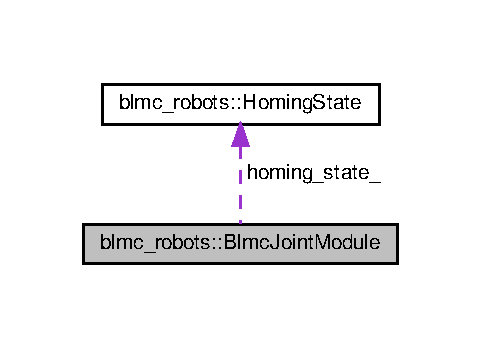
\includegraphics[width=231pt]{classblmc__robots_1_1BlmcJointModule__coll__graph}
\end{center}
\end{figure}
\subsection*{Public Member Functions}
\begin{DoxyCompactItemize}
\item 
\hyperlink{classblmc__robots_1_1BlmcJointModule_a09a0b8815e6c447e3ee6632ade940e0b}{Blmc\+Joint\+Module} (std\+::shared\+\_\+ptr$<$ blmc\+\_\+drivers\+::\+Motor\+Interface $>$ motor, const double \&motor\+\_\+constant, const double \&gear\+\_\+ratio, const double \&zero\+\_\+angle, const bool \&reverse\+\_\+polarity=false, const double \&max\+\_\+current=2.\+1)
\begin{DoxyCompactList}\small\item\em Construct a new \hyperlink{classblmc__robots_1_1BlmcJointModule}{Blmc\+Joint\+Module} object. \end{DoxyCompactList}\item 
void \hyperlink{classblmc__robots_1_1BlmcJointModule_adeb28005a7160ead68603aed4262508f}{set\+\_\+torque} (const double \&desired\+\_\+torque)
\begin{DoxyCompactList}\small\item\em Set the joint torque to be sent. \end{DoxyCompactList}\item 
void \hyperlink{classblmc__robots_1_1BlmcJointModule_ae59680a947539306e391a12ad2d071bb}{set\+\_\+zero\+\_\+angle} (const double \&zero\+\_\+angle)
\begin{DoxyCompactList}\small\item\em Set the zero\+\_\+angle. \end{DoxyCompactList}\item 
void \hyperlink{classblmc__robots_1_1BlmcJointModule_a137da65771a8628db4692e3bfc924f07}{set\+\_\+joint\+\_\+polarity} (const bool \&reverse\+\_\+polarity)
\begin{DoxyCompactList}\small\item\em Define if the motor should turn clock-\/wize or counter clock-\/wize. \end{DoxyCompactList}\item 
void \hyperlink{classblmc__robots_1_1BlmcJointModule_af0484dd9efc47843706fc71d4351bdbd}{send\+\_\+torque} ()
\begin{DoxyCompactList}\small\item\em send the joint torque to the motor. \end{DoxyCompactList}\item 
double \hyperlink{classblmc__robots_1_1BlmcJointModule_a53be7ff5c2b54c15813a68116e85747e}{get\+\_\+max\+\_\+torque} () const
\begin{DoxyCompactList}\small\item\em Get the maximum admissible joint torque that can be applied. \end{DoxyCompactList}\item 
double \hyperlink{classblmc__robots_1_1BlmcJointModule_af3f19ffc942e9b49dce892b207d3d476}{get\+\_\+sent\+\_\+torque} () const
\begin{DoxyCompactList}\small\item\em Get the sent joint torque. \end{DoxyCompactList}\item 
double \hyperlink{classblmc__robots_1_1BlmcJointModule_abb57fdffcc0222b192658239ef45ab63}{get\+\_\+measured\+\_\+torque} () const
\begin{DoxyCompactList}\small\item\em Get the measured joint torque. \end{DoxyCompactList}\item 
double \hyperlink{classblmc__robots_1_1BlmcJointModule_a8c6419cfb80eb5986dffd982df18a817}{get\+\_\+measured\+\_\+angle} () const
\begin{DoxyCompactList}\small\item\em Get the measured angle of the joint. \end{DoxyCompactList}\item 
double \hyperlink{classblmc__robots_1_1BlmcJointModule_a6db4f8c98e9a3e931b19a98dc1339e27}{get\+\_\+measured\+\_\+velocity} () const
\begin{DoxyCompactList}\small\item\em Get the measured velocity of the joint. \end{DoxyCompactList}\item 
double \hyperlink{classblmc__robots_1_1BlmcJointModule_a47b6a71bb9c300d2398924403a6e7e3c}{get\+\_\+measured\+\_\+index\+\_\+angle} () const
\begin{DoxyCompactList}\small\item\em Get the measured index angle. \end{DoxyCompactList}\item 
double \hyperlink{classblmc__robots_1_1BlmcJointModule_ad6fab5bc289e01a34374ea8031f5383e}{get\+\_\+zero\+\_\+angle} () const
\begin{DoxyCompactList}\small\item\em Get the zero\+\_\+angle\+\_\+. \end{DoxyCompactList}\item 
void \hyperlink{classblmc__robots_1_1BlmcJointModule_a464ab2a846630eba6582d09895df2852}{set\+\_\+position\+\_\+control\+\_\+gains} (double kp, double kd)
\begin{DoxyCompactList}\small\item\em Set control gains for PD position controller. \end{DoxyCompactList}\item 
double \hyperlink{classblmc__robots_1_1BlmcJointModule_a3100c088a17264562c67429334e3dbf2}{execute\+\_\+position\+\_\+controller} (double target\+\_\+position\+\_\+rad) const
\begin{DoxyCompactList}\small\item\em Execute one iteration of the position controller. \end{DoxyCompactList}\item 
bool \hyperlink{classblmc__robots_1_1BlmcJointModule_a17a1da041dae31e9a16f955722c36d6c}{calibrate} (double \&angle\+\_\+zero\+\_\+to\+\_\+index, double \&index\+\_\+angle, bool mechanical\+\_\+calibration=false)
\begin{DoxyCompactList}\small\item\em This method calibrate the joint position knowing the angle between the closest (in positive torque) motor index and the theoretical zero pose. \end{DoxyCompactList}\item 
void \hyperlink{classblmc__robots_1_1BlmcJointModule_aa534604b5ead6a3eee5c47a9454f6834}{init\+\_\+homing} (int joint\+\_\+id, double search\+\_\+distance\+\_\+limit\+\_\+rad, double home\+\_\+offset\+\_\+rad, double profile\+\_\+step\+\_\+size\+\_\+rad=0.\+001)
\begin{DoxyCompactList}\small\item\em Initialize the homing procedure. \end{DoxyCompactList}\item 
\hyperlink{blmc__joint__module_8hpp_aa1075809042ff261e4b0a20d161448b6}{Homing\+Return\+Code} \hyperlink{classblmc__robots_1_1BlmcJointModule_abb2712542f3c340bc0ecf76bd343b6b3}{update\+\_\+homing} ()
\begin{DoxyCompactList}\small\item\em Perform one step of homing on encoder index. \end{DoxyCompactList}\item 
double \hyperlink{classblmc__robots_1_1BlmcJointModule_a9fd53d7e340b4067f3505633e5a8a06d}{get\+\_\+distance\+\_\+travelled\+\_\+during\+\_\+homing} () const
\begin{DoxyCompactList}\small\item\em Get distance between start and end position of homing. \end{DoxyCompactList}\end{DoxyCompactItemize}
\subsection*{Private Member Functions}
\begin{DoxyCompactItemize}
\item 
double \hyperlink{classblmc__robots_1_1BlmcJointModule_a2b6886df9dc909854ff74c2ec21cbb34}{joint\+\_\+torque\+\_\+to\+\_\+motor\+\_\+current} (double torque) const
\begin{DoxyCompactList}\small\item\em Convert from joint torque to motor current. \end{DoxyCompactList}\item 
double \hyperlink{classblmc__robots_1_1BlmcJointModule_aa300e4c820a6cd356ac77ba50829c50f}{motor\+\_\+current\+\_\+to\+\_\+joint\+\_\+torque} (double current) const
\begin{DoxyCompactList}\small\item\em Convert from motor current to joint torque. \end{DoxyCompactList}\item 
double \hyperlink{classblmc__robots_1_1BlmcJointModule_a219d4e433d03ea8a2bae115d5563d844}{get\+\_\+motor\+\_\+measurement} (const \hyperlink{common__header_8hpp_a1975c6bb47bc85dfc8edfe349c30dae1}{mi} \&measurement\+\_\+id) const
\begin{DoxyCompactList}\small\item\em Get motor measurements and check if there are data or not. \end{DoxyCompactList}\item 
long int \hyperlink{classblmc__robots_1_1BlmcJointModule_adf5e083076bdc53f24f14f0c22b9061b}{get\+\_\+motor\+\_\+measurement\+\_\+index} (const \hyperlink{common__header_8hpp_a1975c6bb47bc85dfc8edfe349c30dae1}{mi} \&measurement\+\_\+id) const
\begin{DoxyCompactList}\small\item\em Get the last motor measurement index for a specific data. \end{DoxyCompactList}\end{DoxyCompactItemize}
\subsection*{Private Attributes}
\begin{DoxyCompactItemize}
\item 
\mbox{\Hypertarget{classblmc__robots_1_1BlmcJointModule_a0ff5ce1cb26ed04212914dc152ec0486}\label{classblmc__robots_1_1BlmcJointModule_a0ff5ce1cb26ed04212914dc152ec0486}} 
std\+::shared\+\_\+ptr$<$ blmc\+\_\+drivers\+::\+Motor\+Interface $>$ \hyperlink{classblmc__robots_1_1BlmcJointModule_a0ff5ce1cb26ed04212914dc152ec0486}{motor\+\_\+}
\begin{DoxyCompactList}\small\item\em This is the pointer to the motor interface. \end{DoxyCompactList}\item 
\mbox{\Hypertarget{classblmc__robots_1_1BlmcJointModule_a4e2e6f6cc7f0f7aed02efdca60394b40}\label{classblmc__robots_1_1BlmcJointModule_a4e2e6f6cc7f0f7aed02efdca60394b40}} 
double \hyperlink{classblmc__robots_1_1BlmcJointModule_a4e2e6f6cc7f0f7aed02efdca60394b40}{motor\+\_\+constant\+\_\+}
\begin{DoxyCompactList}\small\item\em This is the torque constant of the motor\+: $ \tau_{motor} = k * i_{motor} $. \end{DoxyCompactList}\item 
double \hyperlink{classblmc__robots_1_1BlmcJointModule_af013668d69e7cea2dcc21da8c1c9e4e6}{gear\+\_\+ratio\+\_\+}
\begin{DoxyCompactList}\small\item\em This correspond to the reduction ( $ \beta $) between the motor rotation and the joint. \end{DoxyCompactList}\item 
\mbox{\Hypertarget{classblmc__robots_1_1BlmcJointModule_abdf774193a8ae31486e937eb432dc702}\label{classblmc__robots_1_1BlmcJointModule_abdf774193a8ae31486e937eb432dc702}} 
double \hyperlink{classblmc__robots_1_1BlmcJointModule_abdf774193a8ae31486e937eb432dc702}{zero\+\_\+angle\+\_\+}
\begin{DoxyCompactList}\small\item\em This is the distance between the closest positive index and the zero configuration. \end{DoxyCompactList}\item 
\mbox{\Hypertarget{classblmc__robots_1_1BlmcJointModule_a6ec97901099ebcc3466851624c656f08}\label{classblmc__robots_1_1BlmcJointModule_a6ec97901099ebcc3466851624c656f08}} 
double \hyperlink{classblmc__robots_1_1BlmcJointModule_a6ec97901099ebcc3466851624c656f08}{polarity\+\_\+}
\begin{DoxyCompactList}\small\item\em This change the motor rotation direction. \end{DoxyCompactList}\item 
double \hyperlink{classblmc__robots_1_1BlmcJointModule_af10e1b734a9d4735301962fd9f9c413f}{max\+\_\+current\+\_\+}
\begin{DoxyCompactList}\small\item\em This is the maximum current we can apply during one experiment. \end{DoxyCompactList}\item 
\mbox{\Hypertarget{classblmc__robots_1_1BlmcJointModule_afa5a06b057850fc626649fd13e3f376c}\label{classblmc__robots_1_1BlmcJointModule_afa5a06b057850fc626649fd13e3f376c}} 
double \hyperlink{classblmc__robots_1_1BlmcJointModule_afa5a06b057850fc626649fd13e3f376c}{position\+\_\+control\+\_\+gain\+\_\+p\+\_\+}
\begin{DoxyCompactList}\small\item\em P gain of the position PD controller. \end{DoxyCompactList}\item 
\mbox{\Hypertarget{classblmc__robots_1_1BlmcJointModule_a1141b35d0c53d1f4cca107919c1c861e}\label{classblmc__robots_1_1BlmcJointModule_a1141b35d0c53d1f4cca107919c1c861e}} 
double \hyperlink{classblmc__robots_1_1BlmcJointModule_a1141b35d0c53d1f4cca107919c1c861e}{position\+\_\+control\+\_\+gain\+\_\+d\+\_\+}
\begin{DoxyCompactList}\small\item\em D gain of the position PD controller. \end{DoxyCompactList}\item 
\mbox{\Hypertarget{classblmc__robots_1_1BlmcJointModule_ab7a861d47a808b14e43af7f58ca56284}\label{classblmc__robots_1_1BlmcJointModule_ab7a861d47a808b14e43af7f58ca56284}} 
struct \hyperlink{structblmc__robots_1_1HomingState}{Homing\+State} {\bfseries homing\+\_\+state\+\_\+}
\end{DoxyCompactItemize}


\subsection{Detailed Description}
The \hyperlink{classblmc__robots_1_1BlmcJointModule}{Blmc\+Joint\+Module} class is containing the joint information. 

It is here to help converting the data from the motor side to the joint side. It also allows the calibration of the joint position during initialization. 

\subsection{Constructor \& Destructor Documentation}
\mbox{\Hypertarget{classblmc__robots_1_1BlmcJointModule_a09a0b8815e6c447e3ee6632ade940e0b}\label{classblmc__robots_1_1BlmcJointModule_a09a0b8815e6c447e3ee6632ade940e0b}} 
\index{blmc\+\_\+robots\+::\+Blmc\+Joint\+Module@{blmc\+\_\+robots\+::\+Blmc\+Joint\+Module}!Blmc\+Joint\+Module@{Blmc\+Joint\+Module}}
\index{Blmc\+Joint\+Module@{Blmc\+Joint\+Module}!blmc\+\_\+robots\+::\+Blmc\+Joint\+Module@{blmc\+\_\+robots\+::\+Blmc\+Joint\+Module}}
\subsubsection{\texorpdfstring{Blmc\+Joint\+Module()}{BlmcJointModule()}}
{\footnotesize\ttfamily blmc\+\_\+robots\+::\+Blmc\+Joint\+Module\+::\+Blmc\+Joint\+Module (\begin{DoxyParamCaption}\item[{std\+::shared\+\_\+ptr$<$ blmc\+\_\+drivers\+::\+Motor\+Interface $>$}]{motor,  }\item[{const double \&}]{motor\+\_\+constant,  }\item[{const double \&}]{gear\+\_\+ratio,  }\item[{const double \&}]{zero\+\_\+angle,  }\item[{const bool \&}]{reverse\+\_\+polarity = {\ttfamily false},  }\item[{const double \&}]{max\+\_\+current = {\ttfamily 2.1} }\end{DoxyParamCaption})}



Construct a new \hyperlink{classblmc__robots_1_1BlmcJointModule}{Blmc\+Joint\+Module} object. 


\begin{DoxyParams}{Parameters}
{\em motor} & is the C++ object allowing us to send commands and receive sensor data. \\
\hline
{\em motor\+\_\+constant} & ( $ k $) is the torque constant of the motor $ \tau_{motor} = k * i_{motor} $ \\
\hline
{\em gear\+\_\+ratio} & is the gear ratio between the motor and the joint. \\
\hline
{\em zero\+\_\+angle} & is the angle between the closest positive motor index and the zero configuration. \\
\hline
{\em reverse\+\_\+polarity} & \\
\hline
{\em max\+\_\+current} & \\
\hline
\end{DoxyParams}


\subsection{Member Function Documentation}
\mbox{\Hypertarget{classblmc__robots_1_1BlmcJointModule_a17a1da041dae31e9a16f955722c36d6c}\label{classblmc__robots_1_1BlmcJointModule_a17a1da041dae31e9a16f955722c36d6c}} 
\index{blmc\+\_\+robots\+::\+Blmc\+Joint\+Module@{blmc\+\_\+robots\+::\+Blmc\+Joint\+Module}!calibrate@{calibrate}}
\index{calibrate@{calibrate}!blmc\+\_\+robots\+::\+Blmc\+Joint\+Module@{blmc\+\_\+robots\+::\+Blmc\+Joint\+Module}}
\subsubsection{\texorpdfstring{calibrate()}{calibrate()}}
{\footnotesize\ttfamily bool blmc\+\_\+robots\+::\+Blmc\+Joint\+Module\+::calibrate (\begin{DoxyParamCaption}\item[{double \&}]{angle\+\_\+zero\+\_\+to\+\_\+index,  }\item[{double \&}]{index\+\_\+angle,  }\item[{bool}]{mechanical\+\_\+calibration = {\ttfamily false} }\end{DoxyParamCaption})}



This method calibrate the joint position knowing the angle between the closest (in positive torque) motor index and the theoretical zero pose. 

\begin{DoxyRefDesc}{Deprecated}
\item[\hyperlink{deprecated__deprecated000001}{Deprecated}]!!!!!!! \end{DoxyRefDesc}
Warning, this method should be called in a real time thread!


\begin{DoxyParams}[1]{Parameters}
\mbox{\tt in}  & {\em } & \\
\hline
\end{DoxyParams}
\mbox{\Hypertarget{classblmc__robots_1_1BlmcJointModule_a3100c088a17264562c67429334e3dbf2}\label{classblmc__robots_1_1BlmcJointModule_a3100c088a17264562c67429334e3dbf2}} 
\index{blmc\+\_\+robots\+::\+Blmc\+Joint\+Module@{blmc\+\_\+robots\+::\+Blmc\+Joint\+Module}!execute\+\_\+position\+\_\+controller@{execute\+\_\+position\+\_\+controller}}
\index{execute\+\_\+position\+\_\+controller@{execute\+\_\+position\+\_\+controller}!blmc\+\_\+robots\+::\+Blmc\+Joint\+Module@{blmc\+\_\+robots\+::\+Blmc\+Joint\+Module}}
\subsubsection{\texorpdfstring{execute\+\_\+position\+\_\+controller()}{execute\_position\_controller()}}
{\footnotesize\ttfamily double blmc\+\_\+robots\+::\+Blmc\+Joint\+Module\+::execute\+\_\+position\+\_\+controller (\begin{DoxyParamCaption}\item[{double}]{target\+\_\+position\+\_\+rad }\end{DoxyParamCaption}) const}



Execute one iteration of the position controller. 


\begin{DoxyParams}{Parameters}
{\em target\+\_\+position\+\_\+rad} & Target position (rad).\\
\hline
\end{DoxyParams}
\begin{DoxyReturn}{Returns}
Torque command (Nm). 
\end{DoxyReturn}
\mbox{\Hypertarget{classblmc__robots_1_1BlmcJointModule_a9fd53d7e340b4067f3505633e5a8a06d}\label{classblmc__robots_1_1BlmcJointModule_a9fd53d7e340b4067f3505633e5a8a06d}} 
\index{blmc\+\_\+robots\+::\+Blmc\+Joint\+Module@{blmc\+\_\+robots\+::\+Blmc\+Joint\+Module}!get\+\_\+distance\+\_\+travelled\+\_\+during\+\_\+homing@{get\+\_\+distance\+\_\+travelled\+\_\+during\+\_\+homing}}
\index{get\+\_\+distance\+\_\+travelled\+\_\+during\+\_\+homing@{get\+\_\+distance\+\_\+travelled\+\_\+during\+\_\+homing}!blmc\+\_\+robots\+::\+Blmc\+Joint\+Module@{blmc\+\_\+robots\+::\+Blmc\+Joint\+Module}}
\subsubsection{\texorpdfstring{get\+\_\+distance\+\_\+travelled\+\_\+during\+\_\+homing()}{get\_distance\_travelled\_during\_homing()}}
{\footnotesize\ttfamily double blmc\+\_\+robots\+::\+Blmc\+Joint\+Module\+::get\+\_\+distance\+\_\+travelled\+\_\+during\+\_\+homing (\begin{DoxyParamCaption}{ }\end{DoxyParamCaption}) const}



Get distance between start and end position of homing. 

Compute the distance that the joint moved between initialization of homing and reaching the home position.

This can be used to determine the home offset by first moving the joint to the desired zero position, then executing the homing and finally calling this function which will provide the desired home offset.

\begin{DoxyReturn}{Returns}
Distance between start and end position of homing. 
\end{DoxyReturn}
\mbox{\Hypertarget{classblmc__robots_1_1BlmcJointModule_a53be7ff5c2b54c15813a68116e85747e}\label{classblmc__robots_1_1BlmcJointModule_a53be7ff5c2b54c15813a68116e85747e}} 
\index{blmc\+\_\+robots\+::\+Blmc\+Joint\+Module@{blmc\+\_\+robots\+::\+Blmc\+Joint\+Module}!get\+\_\+max\+\_\+torque@{get\+\_\+max\+\_\+torque}}
\index{get\+\_\+max\+\_\+torque@{get\+\_\+max\+\_\+torque}!blmc\+\_\+robots\+::\+Blmc\+Joint\+Module@{blmc\+\_\+robots\+::\+Blmc\+Joint\+Module}}
\subsubsection{\texorpdfstring{get\+\_\+max\+\_\+torque()}{get\_max\_torque()}}
{\footnotesize\ttfamily double blmc\+\_\+robots\+::\+Blmc\+Joint\+Module\+::get\+\_\+max\+\_\+torque (\begin{DoxyParamCaption}{ }\end{DoxyParamCaption}) const}



Get the maximum admissible joint torque that can be applied. 

\begin{DoxyReturn}{Returns}
double 
\end{DoxyReturn}
\mbox{\Hypertarget{classblmc__robots_1_1BlmcJointModule_a8c6419cfb80eb5986dffd982df18a817}\label{classblmc__robots_1_1BlmcJointModule_a8c6419cfb80eb5986dffd982df18a817}} 
\index{blmc\+\_\+robots\+::\+Blmc\+Joint\+Module@{blmc\+\_\+robots\+::\+Blmc\+Joint\+Module}!get\+\_\+measured\+\_\+angle@{get\+\_\+measured\+\_\+angle}}
\index{get\+\_\+measured\+\_\+angle@{get\+\_\+measured\+\_\+angle}!blmc\+\_\+robots\+::\+Blmc\+Joint\+Module@{blmc\+\_\+robots\+::\+Blmc\+Joint\+Module}}
\subsubsection{\texorpdfstring{get\+\_\+measured\+\_\+angle()}{get\_measured\_angle()}}
{\footnotesize\ttfamily double blmc\+\_\+robots\+::\+Blmc\+Joint\+Module\+::get\+\_\+measured\+\_\+angle (\begin{DoxyParamCaption}{ }\end{DoxyParamCaption}) const}



Get the measured angle of the joint. 

\begin{DoxyReturn}{Returns}
double (rad). 
\end{DoxyReturn}
\mbox{\Hypertarget{classblmc__robots_1_1BlmcJointModule_a47b6a71bb9c300d2398924403a6e7e3c}\label{classblmc__robots_1_1BlmcJointModule_a47b6a71bb9c300d2398924403a6e7e3c}} 
\index{blmc\+\_\+robots\+::\+Blmc\+Joint\+Module@{blmc\+\_\+robots\+::\+Blmc\+Joint\+Module}!get\+\_\+measured\+\_\+index\+\_\+angle@{get\+\_\+measured\+\_\+index\+\_\+angle}}
\index{get\+\_\+measured\+\_\+index\+\_\+angle@{get\+\_\+measured\+\_\+index\+\_\+angle}!blmc\+\_\+robots\+::\+Blmc\+Joint\+Module@{blmc\+\_\+robots\+::\+Blmc\+Joint\+Module}}
\subsubsection{\texorpdfstring{get\+\_\+measured\+\_\+index\+\_\+angle()}{get\_measured\_index\_angle()}}
{\footnotesize\ttfamily double blmc\+\_\+robots\+::\+Blmc\+Joint\+Module\+::get\+\_\+measured\+\_\+index\+\_\+angle (\begin{DoxyParamCaption}{ }\end{DoxyParamCaption}) const}



Get the measured index angle. 

There is one index per motor rotation so there are gear\+\_\+ratio indexes per joint rotation.

\begin{DoxyReturn}{Returns}
double (rad). 
\end{DoxyReturn}
\mbox{\Hypertarget{classblmc__robots_1_1BlmcJointModule_abb57fdffcc0222b192658239ef45ab63}\label{classblmc__robots_1_1BlmcJointModule_abb57fdffcc0222b192658239ef45ab63}} 
\index{blmc\+\_\+robots\+::\+Blmc\+Joint\+Module@{blmc\+\_\+robots\+::\+Blmc\+Joint\+Module}!get\+\_\+measured\+\_\+torque@{get\+\_\+measured\+\_\+torque}}
\index{get\+\_\+measured\+\_\+torque@{get\+\_\+measured\+\_\+torque}!blmc\+\_\+robots\+::\+Blmc\+Joint\+Module@{blmc\+\_\+robots\+::\+Blmc\+Joint\+Module}}
\subsubsection{\texorpdfstring{get\+\_\+measured\+\_\+torque()}{get\_measured\_torque()}}
{\footnotesize\ttfamily double blmc\+\_\+robots\+::\+Blmc\+Joint\+Module\+::get\+\_\+measured\+\_\+torque (\begin{DoxyParamCaption}{ }\end{DoxyParamCaption}) const}



Get the measured joint torque. 

\begin{DoxyReturn}{Returns}
double (Nm). 
\end{DoxyReturn}
\mbox{\Hypertarget{classblmc__robots_1_1BlmcJointModule_a6db4f8c98e9a3e931b19a98dc1339e27}\label{classblmc__robots_1_1BlmcJointModule_a6db4f8c98e9a3e931b19a98dc1339e27}} 
\index{blmc\+\_\+robots\+::\+Blmc\+Joint\+Module@{blmc\+\_\+robots\+::\+Blmc\+Joint\+Module}!get\+\_\+measured\+\_\+velocity@{get\+\_\+measured\+\_\+velocity}}
\index{get\+\_\+measured\+\_\+velocity@{get\+\_\+measured\+\_\+velocity}!blmc\+\_\+robots\+::\+Blmc\+Joint\+Module@{blmc\+\_\+robots\+::\+Blmc\+Joint\+Module}}
\subsubsection{\texorpdfstring{get\+\_\+measured\+\_\+velocity()}{get\_measured\_velocity()}}
{\footnotesize\ttfamily double blmc\+\_\+robots\+::\+Blmc\+Joint\+Module\+::get\+\_\+measured\+\_\+velocity (\begin{DoxyParamCaption}{ }\end{DoxyParamCaption}) const}



Get the measured velocity of the joint. 

This data is computed on board of the control card.

\begin{DoxyReturn}{Returns}
double (rad/s). 
\end{DoxyReturn}
\mbox{\Hypertarget{classblmc__robots_1_1BlmcJointModule_a219d4e433d03ea8a2bae115d5563d844}\label{classblmc__robots_1_1BlmcJointModule_a219d4e433d03ea8a2bae115d5563d844}} 
\index{blmc\+\_\+robots\+::\+Blmc\+Joint\+Module@{blmc\+\_\+robots\+::\+Blmc\+Joint\+Module}!get\+\_\+motor\+\_\+measurement@{get\+\_\+motor\+\_\+measurement}}
\index{get\+\_\+motor\+\_\+measurement@{get\+\_\+motor\+\_\+measurement}!blmc\+\_\+robots\+::\+Blmc\+Joint\+Module@{blmc\+\_\+robots\+::\+Blmc\+Joint\+Module}}
\subsubsection{\texorpdfstring{get\+\_\+motor\+\_\+measurement()}{get\_motor\_measurement()}}
{\footnotesize\ttfamily double blmc\+\_\+robots\+::\+Blmc\+Joint\+Module\+::get\+\_\+motor\+\_\+measurement (\begin{DoxyParamCaption}\item[{const \hyperlink{common__header_8hpp_a1975c6bb47bc85dfc8edfe349c30dae1}{mi} \&}]{measurement\+\_\+id }\end{DoxyParamCaption}) const\hspace{0.3cm}{\ttfamily [private]}}



Get motor measurements and check if there are data or not. 


\begin{DoxyParams}{Parameters}
{\em measurement\+\_\+id} & is the id of the measurement you want to get. check\+: blmc\+\_\+drivers\+::\+Motor\+Interface\+::\+Measurement\+Index \\
\hline
\end{DoxyParams}
\begin{DoxyReturn}{Returns}
double the measurement. 
\end{DoxyReturn}
\mbox{\Hypertarget{classblmc__robots_1_1BlmcJointModule_adf5e083076bdc53f24f14f0c22b9061b}\label{classblmc__robots_1_1BlmcJointModule_adf5e083076bdc53f24f14f0c22b9061b}} 
\index{blmc\+\_\+robots\+::\+Blmc\+Joint\+Module@{blmc\+\_\+robots\+::\+Blmc\+Joint\+Module}!get\+\_\+motor\+\_\+measurement\+\_\+index@{get\+\_\+motor\+\_\+measurement\+\_\+index}}
\index{get\+\_\+motor\+\_\+measurement\+\_\+index@{get\+\_\+motor\+\_\+measurement\+\_\+index}!blmc\+\_\+robots\+::\+Blmc\+Joint\+Module@{blmc\+\_\+robots\+::\+Blmc\+Joint\+Module}}
\subsubsection{\texorpdfstring{get\+\_\+motor\+\_\+measurement\+\_\+index()}{get\_motor\_measurement\_index()}}
{\footnotesize\ttfamily long int blmc\+\_\+robots\+::\+Blmc\+Joint\+Module\+::get\+\_\+motor\+\_\+measurement\+\_\+index (\begin{DoxyParamCaption}\item[{const \hyperlink{common__header_8hpp_a1975c6bb47bc85dfc8edfe349c30dae1}{mi} \&}]{measurement\+\_\+id }\end{DoxyParamCaption}) const\hspace{0.3cm}{\ttfamily [private]}}



Get the last motor measurement index for a specific data. 

If there was no data yet, return NaN


\begin{DoxyParams}{Parameters}
{\em measurement\+\_\+id} & is the id of the measurement you want to get. check\+: blmc\+\_\+drivers\+::\+Motor\+Interface\+::\+Measurement\+Index \\
\hline
\end{DoxyParams}
\begin{DoxyReturn}{Returns}
double the measurement. 
\end{DoxyReturn}
\mbox{\Hypertarget{classblmc__robots_1_1BlmcJointModule_af3f19ffc942e9b49dce892b207d3d476}\label{classblmc__robots_1_1BlmcJointModule_af3f19ffc942e9b49dce892b207d3d476}} 
\index{blmc\+\_\+robots\+::\+Blmc\+Joint\+Module@{blmc\+\_\+robots\+::\+Blmc\+Joint\+Module}!get\+\_\+sent\+\_\+torque@{get\+\_\+sent\+\_\+torque}}
\index{get\+\_\+sent\+\_\+torque@{get\+\_\+sent\+\_\+torque}!blmc\+\_\+robots\+::\+Blmc\+Joint\+Module@{blmc\+\_\+robots\+::\+Blmc\+Joint\+Module}}
\subsubsection{\texorpdfstring{get\+\_\+sent\+\_\+torque()}{get\_sent\_torque()}}
{\footnotesize\ttfamily double blmc\+\_\+robots\+::\+Blmc\+Joint\+Module\+::get\+\_\+sent\+\_\+torque (\begin{DoxyParamCaption}{ }\end{DoxyParamCaption}) const}



Get the sent joint torque. 

\begin{DoxyReturn}{Returns}
double (Nm). 
\end{DoxyReturn}
\mbox{\Hypertarget{classblmc__robots_1_1BlmcJointModule_ad6fab5bc289e01a34374ea8031f5383e}\label{classblmc__robots_1_1BlmcJointModule_ad6fab5bc289e01a34374ea8031f5383e}} 
\index{blmc\+\_\+robots\+::\+Blmc\+Joint\+Module@{blmc\+\_\+robots\+::\+Blmc\+Joint\+Module}!get\+\_\+zero\+\_\+angle@{get\+\_\+zero\+\_\+angle}}
\index{get\+\_\+zero\+\_\+angle@{get\+\_\+zero\+\_\+angle}!blmc\+\_\+robots\+::\+Blmc\+Joint\+Module@{blmc\+\_\+robots\+::\+Blmc\+Joint\+Module}}
\subsubsection{\texorpdfstring{get\+\_\+zero\+\_\+angle()}{get\_zero\_angle()}}
{\footnotesize\ttfamily double blmc\+\_\+robots\+::\+Blmc\+Joint\+Module\+::get\+\_\+zero\+\_\+angle (\begin{DoxyParamCaption}{ }\end{DoxyParamCaption}) const}



Get the zero\+\_\+angle\+\_\+. 

These are the angle between the starting pose and the theoretical zero pose.

\begin{DoxyReturn}{Returns}
double (rad). 
\end{DoxyReturn}
\mbox{\Hypertarget{classblmc__robots_1_1BlmcJointModule_aa534604b5ead6a3eee5c47a9454f6834}\label{classblmc__robots_1_1BlmcJointModule_aa534604b5ead6a3eee5c47a9454f6834}} 
\index{blmc\+\_\+robots\+::\+Blmc\+Joint\+Module@{blmc\+\_\+robots\+::\+Blmc\+Joint\+Module}!init\+\_\+homing@{init\+\_\+homing}}
\index{init\+\_\+homing@{init\+\_\+homing}!blmc\+\_\+robots\+::\+Blmc\+Joint\+Module@{blmc\+\_\+robots\+::\+Blmc\+Joint\+Module}}
\subsubsection{\texorpdfstring{init\+\_\+homing()}{init\_homing()}}
{\footnotesize\ttfamily void blmc\+\_\+robots\+::\+Blmc\+Joint\+Module\+::init\+\_\+homing (\begin{DoxyParamCaption}\item[{int}]{joint\+\_\+id,  }\item[{double}]{search\+\_\+distance\+\_\+limit\+\_\+rad,  }\item[{double}]{home\+\_\+offset\+\_\+rad,  }\item[{double}]{profile\+\_\+step\+\_\+size\+\_\+rad = {\ttfamily 0.001} }\end{DoxyParamCaption})}



Initialize the homing procedure. 

This has to be called before \hyperlink{classblmc__robots_1_1BlmcJointModule_abb2712542f3c340bc0ecf76bd343b6b3}{update\+\_\+homing()}.


\begin{DoxyParams}{Parameters}
{\em joint\+\_\+id} & ID of the joint. This is only used for debug prints. \\
\hline
{\em search\+\_\+distance\+\_\+limit\+\_\+rad} & Maximum distance the motor moves while searching for the encoder index. Unit\+: radian. \\
\hline
{\em home\+\_\+offset\+\_\+rad} & Offset from home position to zero position. Unit\+: radian. \\
\hline
{\em profile\+\_\+step\+\_\+size\+\_\+rad} & Distance by which the target position of the position profile is changed in each step. Set to a negative value to search for the next encoder index in negative direction. Unit\+: radian. \\
\hline
\end{DoxyParams}
\mbox{\Hypertarget{classblmc__robots_1_1BlmcJointModule_a2b6886df9dc909854ff74c2ec21cbb34}\label{classblmc__robots_1_1BlmcJointModule_a2b6886df9dc909854ff74c2ec21cbb34}} 
\index{blmc\+\_\+robots\+::\+Blmc\+Joint\+Module@{blmc\+\_\+robots\+::\+Blmc\+Joint\+Module}!joint\+\_\+torque\+\_\+to\+\_\+motor\+\_\+current@{joint\+\_\+torque\+\_\+to\+\_\+motor\+\_\+current}}
\index{joint\+\_\+torque\+\_\+to\+\_\+motor\+\_\+current@{joint\+\_\+torque\+\_\+to\+\_\+motor\+\_\+current}!blmc\+\_\+robots\+::\+Blmc\+Joint\+Module@{blmc\+\_\+robots\+::\+Blmc\+Joint\+Module}}
\subsubsection{\texorpdfstring{joint\+\_\+torque\+\_\+to\+\_\+motor\+\_\+current()}{joint\_torque\_to\_motor\_current()}}
{\footnotesize\ttfamily double blmc\+\_\+robots\+::\+Blmc\+Joint\+Module\+::joint\+\_\+torque\+\_\+to\+\_\+motor\+\_\+current (\begin{DoxyParamCaption}\item[{double}]{torque }\end{DoxyParamCaption}) const\hspace{0.3cm}{\ttfamily [private]}}



Convert from joint torque to motor current. 


\begin{DoxyParams}[1]{Parameters}
\mbox{\tt in}  & {\em torque} & is the input joint \\
\hline
\end{DoxyParams}
\begin{DoxyReturn}{Returns}
double the equivalent motor current. 
\end{DoxyReturn}
\mbox{\Hypertarget{classblmc__robots_1_1BlmcJointModule_aa300e4c820a6cd356ac77ba50829c50f}\label{classblmc__robots_1_1BlmcJointModule_aa300e4c820a6cd356ac77ba50829c50f}} 
\index{blmc\+\_\+robots\+::\+Blmc\+Joint\+Module@{blmc\+\_\+robots\+::\+Blmc\+Joint\+Module}!motor\+\_\+current\+\_\+to\+\_\+joint\+\_\+torque@{motor\+\_\+current\+\_\+to\+\_\+joint\+\_\+torque}}
\index{motor\+\_\+current\+\_\+to\+\_\+joint\+\_\+torque@{motor\+\_\+current\+\_\+to\+\_\+joint\+\_\+torque}!blmc\+\_\+robots\+::\+Blmc\+Joint\+Module@{blmc\+\_\+robots\+::\+Blmc\+Joint\+Module}}
\subsubsection{\texorpdfstring{motor\+\_\+current\+\_\+to\+\_\+joint\+\_\+torque()}{motor\_current\_to\_joint\_torque()}}
{\footnotesize\ttfamily double blmc\+\_\+robots\+::\+Blmc\+Joint\+Module\+::motor\+\_\+current\+\_\+to\+\_\+joint\+\_\+torque (\begin{DoxyParamCaption}\item[{double}]{current }\end{DoxyParamCaption}) const\hspace{0.3cm}{\ttfamily [private]}}



Convert from motor current to joint torque. 


\begin{DoxyParams}{Parameters}
{\em current} & is the motor current. \\
\hline
\end{DoxyParams}
\begin{DoxyReturn}{Returns}
double is the equivalent joint torque. 
\end{DoxyReturn}
\mbox{\Hypertarget{classblmc__robots_1_1BlmcJointModule_af0484dd9efc47843706fc71d4351bdbd}\label{classblmc__robots_1_1BlmcJointModule_af0484dd9efc47843706fc71d4351bdbd}} 
\index{blmc\+\_\+robots\+::\+Blmc\+Joint\+Module@{blmc\+\_\+robots\+::\+Blmc\+Joint\+Module}!send\+\_\+torque@{send\+\_\+torque}}
\index{send\+\_\+torque@{send\+\_\+torque}!blmc\+\_\+robots\+::\+Blmc\+Joint\+Module@{blmc\+\_\+robots\+::\+Blmc\+Joint\+Module}}
\subsubsection{\texorpdfstring{send\+\_\+torque()}{send\_torque()}}
{\footnotesize\ttfamily void blmc\+\_\+robots\+::\+Blmc\+Joint\+Module\+::send\+\_\+torque (\begin{DoxyParamCaption}{ }\end{DoxyParamCaption})}



send the joint torque to the motor. 

The conversion between joint torque and motor current is done automatically. \mbox{\Hypertarget{classblmc__robots_1_1BlmcJointModule_a137da65771a8628db4692e3bfc924f07}\label{classblmc__robots_1_1BlmcJointModule_a137da65771a8628db4692e3bfc924f07}} 
\index{blmc\+\_\+robots\+::\+Blmc\+Joint\+Module@{blmc\+\_\+robots\+::\+Blmc\+Joint\+Module}!set\+\_\+joint\+\_\+polarity@{set\+\_\+joint\+\_\+polarity}}
\index{set\+\_\+joint\+\_\+polarity@{set\+\_\+joint\+\_\+polarity}!blmc\+\_\+robots\+::\+Blmc\+Joint\+Module@{blmc\+\_\+robots\+::\+Blmc\+Joint\+Module}}
\subsubsection{\texorpdfstring{set\+\_\+joint\+\_\+polarity()}{set\_joint\_polarity()}}
{\footnotesize\ttfamily void blmc\+\_\+robots\+::\+Blmc\+Joint\+Module\+::set\+\_\+joint\+\_\+polarity (\begin{DoxyParamCaption}\item[{const bool \&}]{reverse\+\_\+polarity }\end{DoxyParamCaption})}



Define if the motor should turn clock-\/wize or counter clock-\/wize. 


\begin{DoxyParams}{Parameters}
{\em reverse\+\_\+polarity} & true\+:reverse rotation axis, false\+:do nothing. \\
\hline
\end{DoxyParams}
\mbox{\Hypertarget{classblmc__robots_1_1BlmcJointModule_a464ab2a846630eba6582d09895df2852}\label{classblmc__robots_1_1BlmcJointModule_a464ab2a846630eba6582d09895df2852}} 
\index{blmc\+\_\+robots\+::\+Blmc\+Joint\+Module@{blmc\+\_\+robots\+::\+Blmc\+Joint\+Module}!set\+\_\+position\+\_\+control\+\_\+gains@{set\+\_\+position\+\_\+control\+\_\+gains}}
\index{set\+\_\+position\+\_\+control\+\_\+gains@{set\+\_\+position\+\_\+control\+\_\+gains}!blmc\+\_\+robots\+::\+Blmc\+Joint\+Module@{blmc\+\_\+robots\+::\+Blmc\+Joint\+Module}}
\subsubsection{\texorpdfstring{set\+\_\+position\+\_\+control\+\_\+gains()}{set\_position\_control\_gains()}}
{\footnotesize\ttfamily void blmc\+\_\+robots\+::\+Blmc\+Joint\+Module\+::set\+\_\+position\+\_\+control\+\_\+gains (\begin{DoxyParamCaption}\item[{double}]{kp,  }\item[{double}]{kd }\end{DoxyParamCaption})}



Set control gains for PD position controller. 


\begin{DoxyParams}{Parameters}
{\em kp} & P gain ( (Nm) / rad ). \\
\hline
{\em kd} & D gain ( (Nm) / (rad/s) ). \\
\hline
\end{DoxyParams}
\mbox{\Hypertarget{classblmc__robots_1_1BlmcJointModule_adeb28005a7160ead68603aed4262508f}\label{classblmc__robots_1_1BlmcJointModule_adeb28005a7160ead68603aed4262508f}} 
\index{blmc\+\_\+robots\+::\+Blmc\+Joint\+Module@{blmc\+\_\+robots\+::\+Blmc\+Joint\+Module}!set\+\_\+torque@{set\+\_\+torque}}
\index{set\+\_\+torque@{set\+\_\+torque}!blmc\+\_\+robots\+::\+Blmc\+Joint\+Module@{blmc\+\_\+robots\+::\+Blmc\+Joint\+Module}}
\subsubsection{\texorpdfstring{set\+\_\+torque()}{set\_torque()}}
{\footnotesize\ttfamily void blmc\+\_\+robots\+::\+Blmc\+Joint\+Module\+::set\+\_\+torque (\begin{DoxyParamCaption}\item[{const double \&}]{desired\+\_\+torque }\end{DoxyParamCaption})}



Set the joint torque to be sent. 


\begin{DoxyParams}{Parameters}
{\em desired\+\_\+torque} & (Nm) \\
\hline
\end{DoxyParams}
\mbox{\Hypertarget{classblmc__robots_1_1BlmcJointModule_ae59680a947539306e391a12ad2d071bb}\label{classblmc__robots_1_1BlmcJointModule_ae59680a947539306e391a12ad2d071bb}} 
\index{blmc\+\_\+robots\+::\+Blmc\+Joint\+Module@{blmc\+\_\+robots\+::\+Blmc\+Joint\+Module}!set\+\_\+zero\+\_\+angle@{set\+\_\+zero\+\_\+angle}}
\index{set\+\_\+zero\+\_\+angle@{set\+\_\+zero\+\_\+angle}!blmc\+\_\+robots\+::\+Blmc\+Joint\+Module@{blmc\+\_\+robots\+::\+Blmc\+Joint\+Module}}
\subsubsection{\texorpdfstring{set\+\_\+zero\+\_\+angle()}{set\_zero\_angle()}}
{\footnotesize\ttfamily void blmc\+\_\+robots\+::\+Blmc\+Joint\+Module\+::set\+\_\+zero\+\_\+angle (\begin{DoxyParamCaption}\item[{const double \&}]{zero\+\_\+angle }\end{DoxyParamCaption})}



Set the zero\+\_\+angle. 

The zero\+\_\+angle is the angle between the closest positive motor index and the zero configuration.


\begin{DoxyParams}{Parameters}
{\em zero\+\_\+angle} & (rad) \\
\hline
\end{DoxyParams}
\mbox{\Hypertarget{classblmc__robots_1_1BlmcJointModule_abb2712542f3c340bc0ecf76bd343b6b3}\label{classblmc__robots_1_1BlmcJointModule_abb2712542f3c340bc0ecf76bd343b6b3}} 
\index{blmc\+\_\+robots\+::\+Blmc\+Joint\+Module@{blmc\+\_\+robots\+::\+Blmc\+Joint\+Module}!update\+\_\+homing@{update\+\_\+homing}}
\index{update\+\_\+homing@{update\+\_\+homing}!blmc\+\_\+robots\+::\+Blmc\+Joint\+Module@{blmc\+\_\+robots\+::\+Blmc\+Joint\+Module}}
\subsubsection{\texorpdfstring{update\+\_\+homing()}{update\_homing()}}
{\footnotesize\ttfamily \hyperlink{blmc__joint__module_8hpp_aa1075809042ff261e4b0a20d161448b6}{Homing\+Return\+Code} blmc\+\_\+robots\+::\+Blmc\+Joint\+Module\+::update\+\_\+homing (\begin{DoxyParamCaption}{ }\end{DoxyParamCaption})}



Perform one step of homing on encoder index. 

Searches for the next encoder index in positive direction and, when found, sets it as home position.

Only performs one step, so this method needs to be called in a loop. This method only set the control, one {\itshape M\+U\+ST} send the control for the motor after calling this method.

The motor is moved with a position profile until either the encoder index is reached or the search distance limit is exceeded. The position is controlled with a simple PD controller.

If the encoder index is found, its position is used as home position. The zero position is offset from the home position by adding the \char`\"{}home
offset\char`\"{} to it (i.\+e. zero = home pos. + home offset). If the search distance limit is reached before the encoder index occurs, the homing fails.

\begin{DoxyReturn}{Returns}
Status of the homing procedure. 
\end{DoxyReturn}


\subsection{Member Data Documentation}
\mbox{\Hypertarget{classblmc__robots_1_1BlmcJointModule_af013668d69e7cea2dcc21da8c1c9e4e6}\label{classblmc__robots_1_1BlmcJointModule_af013668d69e7cea2dcc21da8c1c9e4e6}} 
\index{blmc\+\_\+robots\+::\+Blmc\+Joint\+Module@{blmc\+\_\+robots\+::\+Blmc\+Joint\+Module}!gear\+\_\+ratio\+\_\+@{gear\+\_\+ratio\+\_\+}}
\index{gear\+\_\+ratio\+\_\+@{gear\+\_\+ratio\+\_\+}!blmc\+\_\+robots\+::\+Blmc\+Joint\+Module@{blmc\+\_\+robots\+::\+Blmc\+Joint\+Module}}
\subsubsection{\texorpdfstring{gear\+\_\+ratio\+\_\+}{gear\_ratio\_}}
{\footnotesize\ttfamily double blmc\+\_\+robots\+::\+Blmc\+Joint\+Module\+::gear\+\_\+ratio\+\_\+\hspace{0.3cm}{\ttfamily [private]}}



This correspond to the reduction ( $ \beta $) between the motor rotation and the joint. 

$ \theta_{joint} = \theta_{motor} / \beta $ \mbox{\Hypertarget{classblmc__robots_1_1BlmcJointModule_af10e1b734a9d4735301962fd9f9c413f}\label{classblmc__robots_1_1BlmcJointModule_af10e1b734a9d4735301962fd9f9c413f}} 
\index{blmc\+\_\+robots\+::\+Blmc\+Joint\+Module@{blmc\+\_\+robots\+::\+Blmc\+Joint\+Module}!max\+\_\+current\+\_\+@{max\+\_\+current\+\_\+}}
\index{max\+\_\+current\+\_\+@{max\+\_\+current\+\_\+}!blmc\+\_\+robots\+::\+Blmc\+Joint\+Module@{blmc\+\_\+robots\+::\+Blmc\+Joint\+Module}}
\subsubsection{\texorpdfstring{max\+\_\+current\+\_\+}{max\_current\_}}
{\footnotesize\ttfamily double blmc\+\_\+robots\+::\+Blmc\+Joint\+Module\+::max\+\_\+current\+\_\+\hspace{0.3cm}{\ttfamily [private]}}



This is the maximum current we can apply during one experiment. 

The program shut down if this value is achieved. 

The documentation for this class was generated from the following files\+:\begin{DoxyCompactItemize}
\item 
include/blmc\+\_\+robots/\hyperlink{blmc__joint__module_8hpp}{blmc\+\_\+joint\+\_\+module.\+hpp}\item 
src/\hyperlink{blmc__joint__module_8cpp}{blmc\+\_\+joint\+\_\+module.\+cpp}\end{DoxyCompactItemize}

\hypertarget{classblmc__robots_1_1BlmcJointModules}{}\section{blmc\+\_\+robots\+:\+:Blmc\+Joint\+Modules$<$ C\+O\+U\+NT $>$ Class Template Reference}
\label{classblmc__robots_1_1BlmcJointModules}\index{blmc\+\_\+robots\+::\+Blmc\+Joint\+Modules$<$ C\+O\+U\+N\+T $>$@{blmc\+\_\+robots\+::\+Blmc\+Joint\+Modules$<$ C\+O\+U\+N\+T $>$}}


This class defines an interface to a collection of B\+L\+MC joints.  




{\ttfamily \#include $<$blmc\+\_\+joint\+\_\+module.\+hpp$>$}

\subsection*{Public Types}
\begin{DoxyCompactItemize}
\item 
\mbox{\Hypertarget{classblmc__robots_1_1BlmcJointModules_abaff382c6fd4b494ec0c17498d94919e}\label{classblmc__robots_1_1BlmcJointModules_abaff382c6fd4b494ec0c17498d94919e}} 
typedef Eigen\+::\+Matrix$<$ double, C\+O\+U\+NT, 1 $>$ \hyperlink{classblmc__robots_1_1BlmcJointModules_abaff382c6fd4b494ec0c17498d94919e}{Vector}
\begin{DoxyCompactList}\small\item\em Defines a static Eigen vector type in order to define the interface. \end{DoxyCompactList}\end{DoxyCompactItemize}
\subsection*{Public Member Functions}
\begin{DoxyCompactItemize}
\item 
\hyperlink{classblmc__robots_1_1BlmcJointModules_a74910d81a89f9b1713ce8fecc69191fe}{Blmc\+Joint\+Modules} (const std\+::array$<$ std\+::shared\+\_\+ptr$<$ blmc\+\_\+drivers\+::\+Motor\+Interface $>$, C\+O\+U\+NT $>$ \&motors, const \hyperlink{classblmc__robots_1_1BlmcJointModules_abaff382c6fd4b494ec0c17498d94919e}{Vector} \&motor\+\_\+constants, const \hyperlink{classblmc__robots_1_1BlmcJointModules_abaff382c6fd4b494ec0c17498d94919e}{Vector} \&gear\+\_\+ratios, const \hyperlink{classblmc__robots_1_1BlmcJointModules_abaff382c6fd4b494ec0c17498d94919e}{Vector} \&zero\+\_\+angles, const \hyperlink{classblmc__robots_1_1BlmcJointModules_abaff382c6fd4b494ec0c17498d94919e}{Vector} \&max\+\_\+currents)
\begin{DoxyCompactList}\small\item\em Construct a new \hyperlink{classblmc__robots_1_1BlmcJointModules}{Blmc\+Joint\+Modules} object. \end{DoxyCompactList}\item 
\mbox{\Hypertarget{classblmc__robots_1_1BlmcJointModules_af4c700a8d346ceaebece38928b5e7ca6}\label{classblmc__robots_1_1BlmcJointModules_af4c700a8d346ceaebece38928b5e7ca6}} 
\hyperlink{classblmc__robots_1_1BlmcJointModules_af4c700a8d346ceaebece38928b5e7ca6}{Blmc\+Joint\+Modules} ()
\begin{DoxyCompactList}\small\item\em Construct a new \hyperlink{classblmc__robots_1_1BlmcJointModules}{Blmc\+Joint\+Modules} object. \end{DoxyCompactList}\item 
void \hyperlink{classblmc__robots_1_1BlmcJointModules_a905addfe3271be5bc88bd785c5cbb032}{set\+\_\+motor\+\_\+array} (const std\+::array$<$ std\+::shared\+\_\+ptr$<$ blmc\+\_\+drivers\+::\+Motor\+Interface $>$, C\+O\+U\+NT $>$ \&motors, const \hyperlink{classblmc__robots_1_1BlmcJointModules_abaff382c6fd4b494ec0c17498d94919e}{Vector} \&motor\+\_\+constants, const \hyperlink{classblmc__robots_1_1BlmcJointModules_abaff382c6fd4b494ec0c17498d94919e}{Vector} \&gear\+\_\+ratios, const \hyperlink{classblmc__robots_1_1BlmcJointModules_abaff382c6fd4b494ec0c17498d94919e}{Vector} \&zero\+\_\+angles, const \hyperlink{classblmc__robots_1_1BlmcJointModules_abaff382c6fd4b494ec0c17498d94919e}{Vector} \&max\+\_\+currents)
\begin{DoxyCompactList}\small\item\em Set the motor array, by creating the corresponding modules. \end{DoxyCompactList}\item 
\mbox{\Hypertarget{classblmc__robots_1_1BlmcJointModules_a26d4d675142bc783c1f983d135a41a09}\label{classblmc__robots_1_1BlmcJointModules_a26d4d675142bc783c1f983d135a41a09}} 
void \hyperlink{classblmc__robots_1_1BlmcJointModules_a26d4d675142bc783c1f983d135a41a09}{send\+\_\+torques} ()
\begin{DoxyCompactList}\small\item\em Send the registered torques to all modules. \end{DoxyCompactList}\item 
void \hyperlink{classblmc__robots_1_1BlmcJointModules_a97f538c52a1c00846497417333f93230}{set\+\_\+joint\+\_\+polarities} (std\+::array$<$ bool, C\+O\+U\+NT $>$ reverse\+\_\+polarities)
\begin{DoxyCompactList}\small\item\em Set the polarities of the joints (see \hyperlink{classblmc__robots_1_1BlmcJointModule_a137da65771a8628db4692e3bfc924f07}{Blmc\+Joint\+Module\+::set\+\_\+joint\+\_\+polarity}) \end{DoxyCompactList}\item 
void \hyperlink{classblmc__robots_1_1BlmcJointModules_ac7dba81727847238fc4c42b7dca6a0ea}{set\+\_\+torques} (const \hyperlink{classblmc__robots_1_1BlmcJointModules_abaff382c6fd4b494ec0c17498d94919e}{Vector} \&desired\+\_\+torques)
\begin{DoxyCompactList}\small\item\em Register the joint torques to be sent for all modules. \end{DoxyCompactList}\item 
\hyperlink{classblmc__robots_1_1BlmcJointModules_abaff382c6fd4b494ec0c17498d94919e}{Vector} \hyperlink{classblmc__robots_1_1BlmcJointModules_a6cc2989e6132988557ebe03e69658f50}{get\+\_\+max\+\_\+torques} ()
\begin{DoxyCompactList}\small\item\em Get the maximum admissible joint torque that can be applied. \end{DoxyCompactList}\item 
\hyperlink{classblmc__robots_1_1BlmcJointModules_abaff382c6fd4b494ec0c17498d94919e}{Vector} \hyperlink{classblmc__robots_1_1BlmcJointModules_a92f207c6fe5f8fd341b31ef15669fb83}{get\+\_\+sent\+\_\+torques} () const
\begin{DoxyCompactList}\small\item\em Get the previously sent torques. \end{DoxyCompactList}\item 
\hyperlink{classblmc__robots_1_1BlmcJointModules_abaff382c6fd4b494ec0c17498d94919e}{Vector} \hyperlink{classblmc__robots_1_1BlmcJointModules_a24e9a88d03b45f08f9ce0decce7403c0}{get\+\_\+measured\+\_\+torques} () const
\begin{DoxyCompactList}\small\item\em Get the measured joint torques. \end{DoxyCompactList}\item 
\hyperlink{classblmc__robots_1_1BlmcJointModules_abaff382c6fd4b494ec0c17498d94919e}{Vector} \hyperlink{classblmc__robots_1_1BlmcJointModules_abe68677ccf4bdbea975210dcd1de2fdc}{get\+\_\+measured\+\_\+angles} () const
\begin{DoxyCompactList}\small\item\em Get the measured joint angles. \end{DoxyCompactList}\item 
\hyperlink{classblmc__robots_1_1BlmcJointModules_abaff382c6fd4b494ec0c17498d94919e}{Vector} \hyperlink{classblmc__robots_1_1BlmcJointModules_a6138e9e42ce53ce9c5fc7728c5c51558}{get\+\_\+measured\+\_\+velocities} () const
\begin{DoxyCompactList}\small\item\em Get the measured joint velocities. \end{DoxyCompactList}\item 
void \hyperlink{classblmc__robots_1_1BlmcJointModules_abc94960666d33b6a5071d4cf25f7794d}{set\+\_\+zero\+\_\+angles} (const \hyperlink{classblmc__robots_1_1BlmcJointModules_abaff382c6fd4b494ec0c17498d94919e}{Vector} \&zero\+\_\+angles)
\begin{DoxyCompactList}\small\item\em Set the zero\+\_\+angles. \end{DoxyCompactList}\item 
\hyperlink{classblmc__robots_1_1BlmcJointModules_abaff382c6fd4b494ec0c17498d94919e}{Vector} \hyperlink{classblmc__robots_1_1BlmcJointModules_a443404bd864cd2d552e92238a385061a}{get\+\_\+zero\+\_\+angles} () const
\begin{DoxyCompactList}\small\item\em Get the zero\+\_\+angles. \end{DoxyCompactList}\item 
\hyperlink{classblmc__robots_1_1BlmcJointModules_abaff382c6fd4b494ec0c17498d94919e}{Vector} \hyperlink{classblmc__robots_1_1BlmcJointModules_afe8ecc2225292e2a4358b375465b0c93}{get\+\_\+measured\+\_\+index\+\_\+angles} () const
\begin{DoxyCompactList}\small\item\em Get the index\+\_\+angles. \end{DoxyCompactList}\item 
void \hyperlink{classblmc__robots_1_1BlmcJointModules_ada76994634fd0f15fb5df311a61e97d7}{set\+\_\+position\+\_\+control\+\_\+gains} (size\+\_\+t joint\+\_\+id, double kp, double kd)
\begin{DoxyCompactList}\small\item\em Set position control gains for the specified joint. \end{DoxyCompactList}\item 
void \hyperlink{classblmc__robots_1_1BlmcJointModules_a524fd41f808027190d59460a4787aea6}{set\+\_\+position\+\_\+control\+\_\+gains} (\hyperlink{classblmc__robots_1_1BlmcJointModules_abaff382c6fd4b494ec0c17498d94919e}{Vector} kp, \hyperlink{classblmc__robots_1_1BlmcJointModules_abaff382c6fd4b494ec0c17498d94919e}{Vector} kd)
\begin{DoxyCompactList}\small\item\em Set position control gains for all joints. \end{DoxyCompactList}\item 
\hyperlink{blmc__joint__module_8hpp_aa1075809042ff261e4b0a20d161448b6}{Homing\+Return\+Code} \hyperlink{classblmc__robots_1_1BlmcJointModules_a4b3dfee12a87fddf81961fab48e3dae4}{execute\+\_\+homing} (double search\+\_\+distance\+\_\+limit\+\_\+rad, \hyperlink{classblmc__robots_1_1BlmcJointModules_abaff382c6fd4b494ec0c17498d94919e}{Vector} home\+\_\+offset\+\_\+rad, \hyperlink{classblmc__robots_1_1BlmcJointModules_abaff382c6fd4b494ec0c17498d94919e}{Vector} profile\+\_\+step\+\_\+size\+\_\+rad=Vector\+::\+Constant(0.\+001))
\begin{DoxyCompactList}\small\item\em Perform homing for all joints. \end{DoxyCompactList}\item 
\hyperlink{classblmc__robots_1_1BlmcJointModules_abaff382c6fd4b494ec0c17498d94919e}{Vector} \hyperlink{classblmc__robots_1_1BlmcJointModules_afa312ed7c7c5129b547b26b6fa3bab2e}{get\+\_\+distance\+\_\+travelled\+\_\+during\+\_\+homing} () const
\item 
\hyperlink{blmc__joint__module_8hpp_ae2dd8b0230887c948d2583feb6beb051}{Go\+To\+Return\+Code} \hyperlink{classblmc__robots_1_1BlmcJointModules_afc82da986738d3a2265e5cf6337d3251}{go\+\_\+to} (\hyperlink{classblmc__robots_1_1BlmcJointModules_abaff382c6fd4b494ec0c17498d94919e}{Vector} angle\+\_\+to\+\_\+reach\+\_\+rad, double average\+\_\+speed\+\_\+rad\+\_\+per\+\_\+sec=1.\+0)
\begin{DoxyCompactList}\small\item\em Allow the robot to go to a desired pose. \end{DoxyCompactList}\end{DoxyCompactItemize}
\subsection*{Private Attributes}
\begin{DoxyCompactItemize}
\item 
\mbox{\Hypertarget{classblmc__robots_1_1BlmcJointModules_a40ab7b84d3b54d298209098cdf81a14d}\label{classblmc__robots_1_1BlmcJointModules_a40ab7b84d3b54d298209098cdf81a14d}} 
std\+::array$<$ std\+::shared\+\_\+ptr$<$ \hyperlink{classblmc__robots_1_1BlmcJointModule}{Blmc\+Joint\+Module} $>$, C\+O\+U\+NT $>$ \hyperlink{classblmc__robots_1_1BlmcJointModules_a40ab7b84d3b54d298209098cdf81a14d}{modules\+\_\+}
\begin{DoxyCompactList}\small\item\em These are the B\+L\+M\+C\+Joint\+Module objects corresponding to a robot. \end{DoxyCompactList}\end{DoxyCompactItemize}


\subsection{Detailed Description}
\subsubsection*{template$<$int C\+O\+U\+NT$>$\newline
class blmc\+\_\+robots\+::\+Blmc\+Joint\+Modules$<$ C\+O\+U\+N\+T $>$}

This class defines an interface to a collection of B\+L\+MC joints. 

It creates a B\+L\+M\+C\+Joint\+Module for every blmc\+\_\+driver\+::\+Motor\+Interface provided.


\begin{DoxyTemplParams}{Template Parameters}
{\em C\+O\+U\+NT} & \\
\hline
\end{DoxyTemplParams}


\subsection{Constructor \& Destructor Documentation}
\mbox{\Hypertarget{classblmc__robots_1_1BlmcJointModules_a74910d81a89f9b1713ce8fecc69191fe}\label{classblmc__robots_1_1BlmcJointModules_a74910d81a89f9b1713ce8fecc69191fe}} 
\index{blmc\+\_\+robots\+::\+Blmc\+Joint\+Modules@{blmc\+\_\+robots\+::\+Blmc\+Joint\+Modules}!Blmc\+Joint\+Modules@{Blmc\+Joint\+Modules}}
\index{Blmc\+Joint\+Modules@{Blmc\+Joint\+Modules}!blmc\+\_\+robots\+::\+Blmc\+Joint\+Modules@{blmc\+\_\+robots\+::\+Blmc\+Joint\+Modules}}
\subsubsection{\texorpdfstring{Blmc\+Joint\+Modules()}{BlmcJointModules()}}
{\footnotesize\ttfamily template$<$int C\+O\+U\+NT$>$ \\
\hyperlink{classblmc__robots_1_1BlmcJointModules}{blmc\+\_\+robots\+::\+Blmc\+Joint\+Modules}$<$ C\+O\+U\+NT $>$\+::\hyperlink{classblmc__robots_1_1BlmcJointModules}{Blmc\+Joint\+Modules} (\begin{DoxyParamCaption}\item[{const std\+::array$<$ std\+::shared\+\_\+ptr$<$ blmc\+\_\+drivers\+::\+Motor\+Interface $>$, C\+O\+U\+NT $>$ \&}]{motors,  }\item[{const \hyperlink{classblmc__robots_1_1BlmcJointModules_abaff382c6fd4b494ec0c17498d94919e}{Vector} \&}]{motor\+\_\+constants,  }\item[{const \hyperlink{classblmc__robots_1_1BlmcJointModules_abaff382c6fd4b494ec0c17498d94919e}{Vector} \&}]{gear\+\_\+ratios,  }\item[{const \hyperlink{classblmc__robots_1_1BlmcJointModules_abaff382c6fd4b494ec0c17498d94919e}{Vector} \&}]{zero\+\_\+angles,  }\item[{const \hyperlink{classblmc__robots_1_1BlmcJointModules_abaff382c6fd4b494ec0c17498d94919e}{Vector} \&}]{max\+\_\+currents }\end{DoxyParamCaption})\hspace{0.3cm}{\ttfamily [inline]}}



Construct a new \hyperlink{classblmc__robots_1_1BlmcJointModules}{Blmc\+Joint\+Modules} object. 


\begin{DoxyParams}{Parameters}
{\em motors} & \\
\hline
{\em motor\+\_\+constants} & \\
\hline
{\em gear\+\_\+ratios} & \\
\hline
{\em zero\+\_\+angles} & \\
\hline
\end{DoxyParams}


\subsection{Member Function Documentation}
\mbox{\Hypertarget{classblmc__robots_1_1BlmcJointModules_a4b3dfee12a87fddf81961fab48e3dae4}\label{classblmc__robots_1_1BlmcJointModules_a4b3dfee12a87fddf81961fab48e3dae4}} 
\index{blmc\+\_\+robots\+::\+Blmc\+Joint\+Modules@{blmc\+\_\+robots\+::\+Blmc\+Joint\+Modules}!execute\+\_\+homing@{execute\+\_\+homing}}
\index{execute\+\_\+homing@{execute\+\_\+homing}!blmc\+\_\+robots\+::\+Blmc\+Joint\+Modules@{blmc\+\_\+robots\+::\+Blmc\+Joint\+Modules}}
\subsubsection{\texorpdfstring{execute\+\_\+homing()}{execute\_homing()}}
{\footnotesize\ttfamily template$<$int C\+O\+U\+NT$>$ \\
\hyperlink{blmc__joint__module_8hpp_aa1075809042ff261e4b0a20d161448b6}{Homing\+Return\+Code} \hyperlink{classblmc__robots_1_1BlmcJointModules}{blmc\+\_\+robots\+::\+Blmc\+Joint\+Modules}$<$ C\+O\+U\+NT $>$\+::execute\+\_\+homing (\begin{DoxyParamCaption}\item[{double}]{search\+\_\+distance\+\_\+limit\+\_\+rad,  }\item[{\hyperlink{classblmc__robots_1_1BlmcJointModules_abaff382c6fd4b494ec0c17498d94919e}{Vector}}]{home\+\_\+offset\+\_\+rad,  }\item[{\hyperlink{classblmc__robots_1_1BlmcJointModules_abaff382c6fd4b494ec0c17498d94919e}{Vector}}]{profile\+\_\+step\+\_\+size\+\_\+rad = {\ttfamily Vector\+:\+:Constant(0.001)} }\end{DoxyParamCaption})\hspace{0.3cm}{\ttfamily [inline]}}



Perform homing for all joints. 

If one of the joints fails, the complete homing fails. Otherwise it loops until all joints finished. If a joint is finished while others are still running, it is held at the home position.

See \hyperlink{classblmc__robots_1_1BlmcJointModule_abb2712542f3c340bc0ecf76bd343b6b3}{Blmc\+Joint\+Module\+::update\+\_\+homing} for details on the homing procedure.

See \hyperlink{classblmc__robots_1_1BlmcJointModule_aa534604b5ead6a3eee5c47a9454f6834}{Blmc\+Joint\+Module\+::init\+\_\+homing} for description of the arguments.

\begin{DoxyReturn}{Returns}
Final status of the homing procedure (either S\+U\+C\+C\+E\+SS if all joints succeeded or the return code of the first joint that failed). 
\end{DoxyReturn}
\mbox{\Hypertarget{classblmc__robots_1_1BlmcJointModules_afa312ed7c7c5129b547b26b6fa3bab2e}\label{classblmc__robots_1_1BlmcJointModules_afa312ed7c7c5129b547b26b6fa3bab2e}} 
\index{blmc\+\_\+robots\+::\+Blmc\+Joint\+Modules@{blmc\+\_\+robots\+::\+Blmc\+Joint\+Modules}!get\+\_\+distance\+\_\+travelled\+\_\+during\+\_\+homing@{get\+\_\+distance\+\_\+travelled\+\_\+during\+\_\+homing}}
\index{get\+\_\+distance\+\_\+travelled\+\_\+during\+\_\+homing@{get\+\_\+distance\+\_\+travelled\+\_\+during\+\_\+homing}!blmc\+\_\+robots\+::\+Blmc\+Joint\+Modules@{blmc\+\_\+robots\+::\+Blmc\+Joint\+Modules}}
\subsubsection{\texorpdfstring{get\+\_\+distance\+\_\+travelled\+\_\+during\+\_\+homing()}{get\_distance\_travelled\_during\_homing()}}
{\footnotesize\ttfamily template$<$int C\+O\+U\+NT$>$ \\
\hyperlink{classblmc__robots_1_1BlmcJointModules_abaff382c6fd4b494ec0c17498d94919e}{Vector} \hyperlink{classblmc__robots_1_1BlmcJointModules}{blmc\+\_\+robots\+::\+Blmc\+Joint\+Modules}$<$ C\+O\+U\+NT $>$\+::get\+\_\+distance\+\_\+travelled\+\_\+during\+\_\+homing (\begin{DoxyParamCaption}{ }\end{DoxyParamCaption}) const\hspace{0.3cm}{\ttfamily [inline]}}

\begin{DoxySeeAlso}{See also}
\hyperlink{classblmc__robots_1_1BlmcJointModule_a9fd53d7e340b4067f3505633e5a8a06d}{Blmc\+Joint\+Module\+::get\+\_\+distance\+\_\+travelled\+\_\+during\+\_\+homing} 
\end{DoxySeeAlso}
\mbox{\Hypertarget{classblmc__robots_1_1BlmcJointModules_a6cc2989e6132988557ebe03e69658f50}\label{classblmc__robots_1_1BlmcJointModules_a6cc2989e6132988557ebe03e69658f50}} 
\index{blmc\+\_\+robots\+::\+Blmc\+Joint\+Modules@{blmc\+\_\+robots\+::\+Blmc\+Joint\+Modules}!get\+\_\+max\+\_\+torques@{get\+\_\+max\+\_\+torques}}
\index{get\+\_\+max\+\_\+torques@{get\+\_\+max\+\_\+torques}!blmc\+\_\+robots\+::\+Blmc\+Joint\+Modules@{blmc\+\_\+robots\+::\+Blmc\+Joint\+Modules}}
\subsubsection{\texorpdfstring{get\+\_\+max\+\_\+torques()}{get\_max\_torques()}}
{\footnotesize\ttfamily template$<$int C\+O\+U\+NT$>$ \\
\hyperlink{classblmc__robots_1_1BlmcJointModules_abaff382c6fd4b494ec0c17498d94919e}{Vector} \hyperlink{classblmc__robots_1_1BlmcJointModules}{blmc\+\_\+robots\+::\+Blmc\+Joint\+Modules}$<$ C\+O\+U\+NT $>$\+::get\+\_\+max\+\_\+torques (\begin{DoxyParamCaption}{ }\end{DoxyParamCaption})\hspace{0.3cm}{\ttfamily [inline]}}



Get the maximum admissible joint torque that can be applied. 

\begin{DoxyReturn}{Returns}
Vector (N/m) 
\end{DoxyReturn}
\mbox{\Hypertarget{classblmc__robots_1_1BlmcJointModules_abe68677ccf4bdbea975210dcd1de2fdc}\label{classblmc__robots_1_1BlmcJointModules_abe68677ccf4bdbea975210dcd1de2fdc}} 
\index{blmc\+\_\+robots\+::\+Blmc\+Joint\+Modules@{blmc\+\_\+robots\+::\+Blmc\+Joint\+Modules}!get\+\_\+measured\+\_\+angles@{get\+\_\+measured\+\_\+angles}}
\index{get\+\_\+measured\+\_\+angles@{get\+\_\+measured\+\_\+angles}!blmc\+\_\+robots\+::\+Blmc\+Joint\+Modules@{blmc\+\_\+robots\+::\+Blmc\+Joint\+Modules}}
\subsubsection{\texorpdfstring{get\+\_\+measured\+\_\+angles()}{get\_measured\_angles()}}
{\footnotesize\ttfamily template$<$int C\+O\+U\+NT$>$ \\
\hyperlink{classblmc__robots_1_1BlmcJointModules_abaff382c6fd4b494ec0c17498d94919e}{Vector} \hyperlink{classblmc__robots_1_1BlmcJointModules}{blmc\+\_\+robots\+::\+Blmc\+Joint\+Modules}$<$ C\+O\+U\+NT $>$\+::get\+\_\+measured\+\_\+angles (\begin{DoxyParamCaption}{ }\end{DoxyParamCaption}) const\hspace{0.3cm}{\ttfamily [inline]}}



Get the measured joint angles. 

\begin{DoxyReturn}{Returns}
Vector (rad) 
\end{DoxyReturn}
\mbox{\Hypertarget{classblmc__robots_1_1BlmcJointModules_afe8ecc2225292e2a4358b375465b0c93}\label{classblmc__robots_1_1BlmcJointModules_afe8ecc2225292e2a4358b375465b0c93}} 
\index{blmc\+\_\+robots\+::\+Blmc\+Joint\+Modules@{blmc\+\_\+robots\+::\+Blmc\+Joint\+Modules}!get\+\_\+measured\+\_\+index\+\_\+angles@{get\+\_\+measured\+\_\+index\+\_\+angles}}
\index{get\+\_\+measured\+\_\+index\+\_\+angles@{get\+\_\+measured\+\_\+index\+\_\+angles}!blmc\+\_\+robots\+::\+Blmc\+Joint\+Modules@{blmc\+\_\+robots\+::\+Blmc\+Joint\+Modules}}
\subsubsection{\texorpdfstring{get\+\_\+measured\+\_\+index\+\_\+angles()}{get\_measured\_index\_angles()}}
{\footnotesize\ttfamily template$<$int C\+O\+U\+NT$>$ \\
\hyperlink{classblmc__robots_1_1BlmcJointModules_abaff382c6fd4b494ec0c17498d94919e}{Vector} \hyperlink{classblmc__robots_1_1BlmcJointModules}{blmc\+\_\+robots\+::\+Blmc\+Joint\+Modules}$<$ C\+O\+U\+NT $>$\+::get\+\_\+measured\+\_\+index\+\_\+angles (\begin{DoxyParamCaption}{ }\end{DoxyParamCaption}) const\hspace{0.3cm}{\ttfamily [inline]}}



Get the index\+\_\+angles. 

There is one index per motor rotation so there are gear\+\_\+ratio indexes per joint rotation.

\begin{DoxyReturn}{Returns}
Vector (rad) 
\end{DoxyReturn}
\mbox{\Hypertarget{classblmc__robots_1_1BlmcJointModules_a24e9a88d03b45f08f9ce0decce7403c0}\label{classblmc__robots_1_1BlmcJointModules_a24e9a88d03b45f08f9ce0decce7403c0}} 
\index{blmc\+\_\+robots\+::\+Blmc\+Joint\+Modules@{blmc\+\_\+robots\+::\+Blmc\+Joint\+Modules}!get\+\_\+measured\+\_\+torques@{get\+\_\+measured\+\_\+torques}}
\index{get\+\_\+measured\+\_\+torques@{get\+\_\+measured\+\_\+torques}!blmc\+\_\+robots\+::\+Blmc\+Joint\+Modules@{blmc\+\_\+robots\+::\+Blmc\+Joint\+Modules}}
\subsubsection{\texorpdfstring{get\+\_\+measured\+\_\+torques()}{get\_measured\_torques()}}
{\footnotesize\ttfamily template$<$int C\+O\+U\+NT$>$ \\
\hyperlink{classblmc__robots_1_1BlmcJointModules_abaff382c6fd4b494ec0c17498d94919e}{Vector} \hyperlink{classblmc__robots_1_1BlmcJointModules}{blmc\+\_\+robots\+::\+Blmc\+Joint\+Modules}$<$ C\+O\+U\+NT $>$\+::get\+\_\+measured\+\_\+torques (\begin{DoxyParamCaption}{ }\end{DoxyParamCaption}) const\hspace{0.3cm}{\ttfamily [inline]}}



Get the measured joint torques. 

\begin{DoxyReturn}{Returns}
Vector (Nm) 
\end{DoxyReturn}
\mbox{\Hypertarget{classblmc__robots_1_1BlmcJointModules_a6138e9e42ce53ce9c5fc7728c5c51558}\label{classblmc__robots_1_1BlmcJointModules_a6138e9e42ce53ce9c5fc7728c5c51558}} 
\index{blmc\+\_\+robots\+::\+Blmc\+Joint\+Modules@{blmc\+\_\+robots\+::\+Blmc\+Joint\+Modules}!get\+\_\+measured\+\_\+velocities@{get\+\_\+measured\+\_\+velocities}}
\index{get\+\_\+measured\+\_\+velocities@{get\+\_\+measured\+\_\+velocities}!blmc\+\_\+robots\+::\+Blmc\+Joint\+Modules@{blmc\+\_\+robots\+::\+Blmc\+Joint\+Modules}}
\subsubsection{\texorpdfstring{get\+\_\+measured\+\_\+velocities()}{get\_measured\_velocities()}}
{\footnotesize\ttfamily template$<$int C\+O\+U\+NT$>$ \\
\hyperlink{classblmc__robots_1_1BlmcJointModules_abaff382c6fd4b494ec0c17498d94919e}{Vector} \hyperlink{classblmc__robots_1_1BlmcJointModules}{blmc\+\_\+robots\+::\+Blmc\+Joint\+Modules}$<$ C\+O\+U\+NT $>$\+::get\+\_\+measured\+\_\+velocities (\begin{DoxyParamCaption}{ }\end{DoxyParamCaption}) const\hspace{0.3cm}{\ttfamily [inline]}}



Get the measured joint velocities. 

\begin{DoxyReturn}{Returns}
Vector (rad/s) 
\end{DoxyReturn}
\mbox{\Hypertarget{classblmc__robots_1_1BlmcJointModules_a92f207c6fe5f8fd341b31ef15669fb83}\label{classblmc__robots_1_1BlmcJointModules_a92f207c6fe5f8fd341b31ef15669fb83}} 
\index{blmc\+\_\+robots\+::\+Blmc\+Joint\+Modules@{blmc\+\_\+robots\+::\+Blmc\+Joint\+Modules}!get\+\_\+sent\+\_\+torques@{get\+\_\+sent\+\_\+torques}}
\index{get\+\_\+sent\+\_\+torques@{get\+\_\+sent\+\_\+torques}!blmc\+\_\+robots\+::\+Blmc\+Joint\+Modules@{blmc\+\_\+robots\+::\+Blmc\+Joint\+Modules}}
\subsubsection{\texorpdfstring{get\+\_\+sent\+\_\+torques()}{get\_sent\_torques()}}
{\footnotesize\ttfamily template$<$int C\+O\+U\+NT$>$ \\
\hyperlink{classblmc__robots_1_1BlmcJointModules_abaff382c6fd4b494ec0c17498d94919e}{Vector} \hyperlink{classblmc__robots_1_1BlmcJointModules}{blmc\+\_\+robots\+::\+Blmc\+Joint\+Modules}$<$ C\+O\+U\+NT $>$\+::get\+\_\+sent\+\_\+torques (\begin{DoxyParamCaption}{ }\end{DoxyParamCaption}) const\hspace{0.3cm}{\ttfamily [inline]}}



Get the previously sent torques. 

\begin{DoxyReturn}{Returns}
Vector (Nm) 
\end{DoxyReturn}
\mbox{\Hypertarget{classblmc__robots_1_1BlmcJointModules_a443404bd864cd2d552e92238a385061a}\label{classblmc__robots_1_1BlmcJointModules_a443404bd864cd2d552e92238a385061a}} 
\index{blmc\+\_\+robots\+::\+Blmc\+Joint\+Modules@{blmc\+\_\+robots\+::\+Blmc\+Joint\+Modules}!get\+\_\+zero\+\_\+angles@{get\+\_\+zero\+\_\+angles}}
\index{get\+\_\+zero\+\_\+angles@{get\+\_\+zero\+\_\+angles}!blmc\+\_\+robots\+::\+Blmc\+Joint\+Modules@{blmc\+\_\+robots\+::\+Blmc\+Joint\+Modules}}
\subsubsection{\texorpdfstring{get\+\_\+zero\+\_\+angles()}{get\_zero\_angles()}}
{\footnotesize\ttfamily template$<$int C\+O\+U\+NT$>$ \\
\hyperlink{classblmc__robots_1_1BlmcJointModules_abaff382c6fd4b494ec0c17498d94919e}{Vector} \hyperlink{classblmc__robots_1_1BlmcJointModules}{blmc\+\_\+robots\+::\+Blmc\+Joint\+Modules}$<$ C\+O\+U\+NT $>$\+::get\+\_\+zero\+\_\+angles (\begin{DoxyParamCaption}{ }\end{DoxyParamCaption}) const\hspace{0.3cm}{\ttfamily [inline]}}



Get the zero\+\_\+angles. 

These are the joint angles between the starting pose and the zero theoretical pose of the urdf.

\begin{DoxyReturn}{Returns}
Vector (rad) 
\end{DoxyReturn}
\mbox{\Hypertarget{classblmc__robots_1_1BlmcJointModules_afc82da986738d3a2265e5cf6337d3251}\label{classblmc__robots_1_1BlmcJointModules_afc82da986738d3a2265e5cf6337d3251}} 
\index{blmc\+\_\+robots\+::\+Blmc\+Joint\+Modules@{blmc\+\_\+robots\+::\+Blmc\+Joint\+Modules}!go\+\_\+to@{go\+\_\+to}}
\index{go\+\_\+to@{go\+\_\+to}!blmc\+\_\+robots\+::\+Blmc\+Joint\+Modules@{blmc\+\_\+robots\+::\+Blmc\+Joint\+Modules}}
\subsubsection{\texorpdfstring{go\+\_\+to()}{go\_to()}}
{\footnotesize\ttfamily template$<$int C\+O\+U\+NT$>$ \\
\hyperlink{blmc__joint__module_8hpp_ae2dd8b0230887c948d2583feb6beb051}{Go\+To\+Return\+Code} \hyperlink{classblmc__robots_1_1BlmcJointModules}{blmc\+\_\+robots\+::\+Blmc\+Joint\+Modules}$<$ C\+O\+U\+NT $>$\+::go\+\_\+to (\begin{DoxyParamCaption}\item[{\hyperlink{classblmc__robots_1_1BlmcJointModules_abaff382c6fd4b494ec0c17498d94919e}{Vector}}]{angle\+\_\+to\+\_\+reach\+\_\+rad,  }\item[{double}]{average\+\_\+speed\+\_\+rad\+\_\+per\+\_\+sec = {\ttfamily 1.0} }\end{DoxyParamCaption})\hspace{0.3cm}{\ttfamily [inline]}}



Allow the robot to go to a desired pose. 

Once the control done 0 torques is sent.


\begin{DoxyParams}{Parameters}
{\em angle\+\_\+to\+\_\+reach\+\_\+rad} & (rad) \\
\hline
{\em average\+\_\+speed\+\_\+rad\+\_\+per\+\_\+sec} & (rad/sec) \\
\hline
\end{DoxyParams}
\begin{DoxyReturn}{Returns}
Go\+To\+Return\+Code 
\end{DoxyReturn}
\mbox{\Hypertarget{classblmc__robots_1_1BlmcJointModules_a97f538c52a1c00846497417333f93230}\label{classblmc__robots_1_1BlmcJointModules_a97f538c52a1c00846497417333f93230}} 
\index{blmc\+\_\+robots\+::\+Blmc\+Joint\+Modules@{blmc\+\_\+robots\+::\+Blmc\+Joint\+Modules}!set\+\_\+joint\+\_\+polarities@{set\+\_\+joint\+\_\+polarities}}
\index{set\+\_\+joint\+\_\+polarities@{set\+\_\+joint\+\_\+polarities}!blmc\+\_\+robots\+::\+Blmc\+Joint\+Modules@{blmc\+\_\+robots\+::\+Blmc\+Joint\+Modules}}
\subsubsection{\texorpdfstring{set\+\_\+joint\+\_\+polarities()}{set\_joint\_polarities()}}
{\footnotesize\ttfamily template$<$int C\+O\+U\+NT$>$ \\
void \hyperlink{classblmc__robots_1_1BlmcJointModules}{blmc\+\_\+robots\+::\+Blmc\+Joint\+Modules}$<$ C\+O\+U\+NT $>$\+::set\+\_\+joint\+\_\+polarities (\begin{DoxyParamCaption}\item[{std\+::array$<$ bool, C\+O\+U\+NT $>$}]{reverse\+\_\+polarities }\end{DoxyParamCaption})\hspace{0.3cm}{\ttfamily [inline]}}



Set the polarities of the joints (see \hyperlink{classblmc__robots_1_1BlmcJointModule_a137da65771a8628db4692e3bfc924f07}{Blmc\+Joint\+Module\+::set\+\_\+joint\+\_\+polarity}) 


\begin{DoxyParams}{Parameters}
{\em reverse\+\_\+polarity} & \\
\hline
\end{DoxyParams}
\mbox{\Hypertarget{classblmc__robots_1_1BlmcJointModules_a905addfe3271be5bc88bd785c5cbb032}\label{classblmc__robots_1_1BlmcJointModules_a905addfe3271be5bc88bd785c5cbb032}} 
\index{blmc\+\_\+robots\+::\+Blmc\+Joint\+Modules@{blmc\+\_\+robots\+::\+Blmc\+Joint\+Modules}!set\+\_\+motor\+\_\+array@{set\+\_\+motor\+\_\+array}}
\index{set\+\_\+motor\+\_\+array@{set\+\_\+motor\+\_\+array}!blmc\+\_\+robots\+::\+Blmc\+Joint\+Modules@{blmc\+\_\+robots\+::\+Blmc\+Joint\+Modules}}
\subsubsection{\texorpdfstring{set\+\_\+motor\+\_\+array()}{set\_motor\_array()}}
{\footnotesize\ttfamily template$<$int C\+O\+U\+NT$>$ \\
void \hyperlink{classblmc__robots_1_1BlmcJointModules}{blmc\+\_\+robots\+::\+Blmc\+Joint\+Modules}$<$ C\+O\+U\+NT $>$\+::set\+\_\+motor\+\_\+array (\begin{DoxyParamCaption}\item[{const std\+::array$<$ std\+::shared\+\_\+ptr$<$ blmc\+\_\+drivers\+::\+Motor\+Interface $>$, C\+O\+U\+NT $>$ \&}]{motors,  }\item[{const \hyperlink{classblmc__robots_1_1BlmcJointModules_abaff382c6fd4b494ec0c17498d94919e}{Vector} \&}]{motor\+\_\+constants,  }\item[{const \hyperlink{classblmc__robots_1_1BlmcJointModules_abaff382c6fd4b494ec0c17498d94919e}{Vector} \&}]{gear\+\_\+ratios,  }\item[{const \hyperlink{classblmc__robots_1_1BlmcJointModules_abaff382c6fd4b494ec0c17498d94919e}{Vector} \&}]{zero\+\_\+angles,  }\item[{const \hyperlink{classblmc__robots_1_1BlmcJointModules_abaff382c6fd4b494ec0c17498d94919e}{Vector} \&}]{max\+\_\+currents }\end{DoxyParamCaption})\hspace{0.3cm}{\ttfamily [inline]}}



Set the motor array, by creating the corresponding modules. 


\begin{DoxyParams}{Parameters}
{\em motors} & \\
\hline
{\em motor\+\_\+constants} & \\
\hline
{\em gear\+\_\+ratios} & \\
\hline
{\em zero\+\_\+angles} & \\
\hline
\end{DoxyParams}
\mbox{\Hypertarget{classblmc__robots_1_1BlmcJointModules_ada76994634fd0f15fb5df311a61e97d7}\label{classblmc__robots_1_1BlmcJointModules_ada76994634fd0f15fb5df311a61e97d7}} 
\index{blmc\+\_\+robots\+::\+Blmc\+Joint\+Modules@{blmc\+\_\+robots\+::\+Blmc\+Joint\+Modules}!set\+\_\+position\+\_\+control\+\_\+gains@{set\+\_\+position\+\_\+control\+\_\+gains}}
\index{set\+\_\+position\+\_\+control\+\_\+gains@{set\+\_\+position\+\_\+control\+\_\+gains}!blmc\+\_\+robots\+::\+Blmc\+Joint\+Modules@{blmc\+\_\+robots\+::\+Blmc\+Joint\+Modules}}
\subsubsection{\texorpdfstring{set\+\_\+position\+\_\+control\+\_\+gains()}{set\_position\_control\_gains()}\hspace{0.1cm}{\footnotesize\ttfamily [1/2]}}
{\footnotesize\ttfamily template$<$int C\+O\+U\+NT$>$ \\
void \hyperlink{classblmc__robots_1_1BlmcJointModules}{blmc\+\_\+robots\+::\+Blmc\+Joint\+Modules}$<$ C\+O\+U\+NT $>$\+::set\+\_\+position\+\_\+control\+\_\+gains (\begin{DoxyParamCaption}\item[{size\+\_\+t}]{joint\+\_\+id,  }\item[{double}]{kp,  }\item[{double}]{kd }\end{DoxyParamCaption})\hspace{0.3cm}{\ttfamily [inline]}}



Set position control gains for the specified joint. 


\begin{DoxyParams}{Parameters}
{\em joint\+\_\+id} & ID of the joint (in range {\ttfamily \mbox{[}0, C\+O\+U\+NT)}). \\
\hline
{\em kp} & P gain. \\
\hline
{\em kd} & D gain. \\
\hline
\end{DoxyParams}
\mbox{\Hypertarget{classblmc__robots_1_1BlmcJointModules_a524fd41f808027190d59460a4787aea6}\label{classblmc__robots_1_1BlmcJointModules_a524fd41f808027190d59460a4787aea6}} 
\index{blmc\+\_\+robots\+::\+Blmc\+Joint\+Modules@{blmc\+\_\+robots\+::\+Blmc\+Joint\+Modules}!set\+\_\+position\+\_\+control\+\_\+gains@{set\+\_\+position\+\_\+control\+\_\+gains}}
\index{set\+\_\+position\+\_\+control\+\_\+gains@{set\+\_\+position\+\_\+control\+\_\+gains}!blmc\+\_\+robots\+::\+Blmc\+Joint\+Modules@{blmc\+\_\+robots\+::\+Blmc\+Joint\+Modules}}
\subsubsection{\texorpdfstring{set\+\_\+position\+\_\+control\+\_\+gains()}{set\_position\_control\_gains()}\hspace{0.1cm}{\footnotesize\ttfamily [2/2]}}
{\footnotesize\ttfamily template$<$int C\+O\+U\+NT$>$ \\
void \hyperlink{classblmc__robots_1_1BlmcJointModules}{blmc\+\_\+robots\+::\+Blmc\+Joint\+Modules}$<$ C\+O\+U\+NT $>$\+::set\+\_\+position\+\_\+control\+\_\+gains (\begin{DoxyParamCaption}\item[{\hyperlink{classblmc__robots_1_1BlmcJointModules_abaff382c6fd4b494ec0c17498d94919e}{Vector}}]{kp,  }\item[{\hyperlink{classblmc__robots_1_1BlmcJointModules_abaff382c6fd4b494ec0c17498d94919e}{Vector}}]{kd }\end{DoxyParamCaption})\hspace{0.3cm}{\ttfamily [inline]}}



Set position control gains for all joints. 


\begin{DoxyParams}{Parameters}
{\em kp} & P gains. \\
\hline
{\em kd} & D gains. \\
\hline
\end{DoxyParams}
\mbox{\Hypertarget{classblmc__robots_1_1BlmcJointModules_ac7dba81727847238fc4c42b7dca6a0ea}\label{classblmc__robots_1_1BlmcJointModules_ac7dba81727847238fc4c42b7dca6a0ea}} 
\index{blmc\+\_\+robots\+::\+Blmc\+Joint\+Modules@{blmc\+\_\+robots\+::\+Blmc\+Joint\+Modules}!set\+\_\+torques@{set\+\_\+torques}}
\index{set\+\_\+torques@{set\+\_\+torques}!blmc\+\_\+robots\+::\+Blmc\+Joint\+Modules@{blmc\+\_\+robots\+::\+Blmc\+Joint\+Modules}}
\subsubsection{\texorpdfstring{set\+\_\+torques()}{set\_torques()}}
{\footnotesize\ttfamily template$<$int C\+O\+U\+NT$>$ \\
void \hyperlink{classblmc__robots_1_1BlmcJointModules}{blmc\+\_\+robots\+::\+Blmc\+Joint\+Modules}$<$ C\+O\+U\+NT $>$\+::set\+\_\+torques (\begin{DoxyParamCaption}\item[{const \hyperlink{classblmc__robots_1_1BlmcJointModules_abaff382c6fd4b494ec0c17498d94919e}{Vector} \&}]{desired\+\_\+torques }\end{DoxyParamCaption})\hspace{0.3cm}{\ttfamily [inline]}}



Register the joint torques to be sent for all modules. 


\begin{DoxyParams}{Parameters}
{\em desired\+\_\+torques} & (Nm) \\
\hline
\end{DoxyParams}
\mbox{\Hypertarget{classblmc__robots_1_1BlmcJointModules_abc94960666d33b6a5071d4cf25f7794d}\label{classblmc__robots_1_1BlmcJointModules_abc94960666d33b6a5071d4cf25f7794d}} 
\index{blmc\+\_\+robots\+::\+Blmc\+Joint\+Modules@{blmc\+\_\+robots\+::\+Blmc\+Joint\+Modules}!set\+\_\+zero\+\_\+angles@{set\+\_\+zero\+\_\+angles}}
\index{set\+\_\+zero\+\_\+angles@{set\+\_\+zero\+\_\+angles}!blmc\+\_\+robots\+::\+Blmc\+Joint\+Modules@{blmc\+\_\+robots\+::\+Blmc\+Joint\+Modules}}
\subsubsection{\texorpdfstring{set\+\_\+zero\+\_\+angles()}{set\_zero\_angles()}}
{\footnotesize\ttfamily template$<$int C\+O\+U\+NT$>$ \\
void \hyperlink{classblmc__robots_1_1BlmcJointModules}{blmc\+\_\+robots\+::\+Blmc\+Joint\+Modules}$<$ C\+O\+U\+NT $>$\+::set\+\_\+zero\+\_\+angles (\begin{DoxyParamCaption}\item[{const \hyperlink{classblmc__robots_1_1BlmcJointModules_abaff382c6fd4b494ec0c17498d94919e}{Vector} \&}]{zero\+\_\+angles }\end{DoxyParamCaption})\hspace{0.3cm}{\ttfamily [inline]}}



Set the zero\+\_\+angles. 

These are the joint angles between the starting pose and the zero theoretical pose of the urdf.


\begin{DoxyParams}{Parameters}
{\em zero\+\_\+angles} & (rad) \\
\hline
\end{DoxyParams}


The documentation for this class was generated from the following file\+:\begin{DoxyCompactItemize}
\item 
include/blmc\+\_\+robots/\hyperlink{blmc__joint__module_8hpp}{blmc\+\_\+joint\+\_\+module.\+hpp}\end{DoxyCompactItemize}

\hypertarget{structblmc__robots_1_1NJointBlmcRobotDriver_1_1Config}{}\section{blmc\+\_\+robots\+:\+:N\+Joint\+Blmc\+Robot\+Driver$<$ Observation, N\+\_\+\+J\+O\+I\+N\+TS, N\+\_\+\+M\+O\+T\+O\+R\+\_\+\+B\+O\+A\+R\+DS $>$\+:\+:Config Struct Reference}
\label{structblmc__robots_1_1NJointBlmcRobotDriver_1_1Config}\index{blmc\+\_\+robots\+::\+N\+Joint\+Blmc\+Robot\+Driver$<$ Observation, N\+\_\+\+J\+O\+I\+N\+T\+S, N\+\_\+\+M\+O\+T\+O\+R\+\_\+\+B\+O\+A\+R\+D\+S $>$\+::\+Config@{blmc\+\_\+robots\+::\+N\+Joint\+Blmc\+Robot\+Driver$<$ Observation, N\+\_\+\+J\+O\+I\+N\+T\+S, N\+\_\+\+M\+O\+T\+O\+R\+\_\+\+B\+O\+A\+R\+D\+S $>$\+::\+Config}}


Configuration of the robot that can be changed by the user.  




{\ttfamily \#include $<$n\+\_\+joint\+\_\+blmc\+\_\+robot\+\_\+driver.\+hpp$>$}

\subsection*{Classes}
\begin{DoxyCompactItemize}
\item 
struct \hyperlink{structblmc__robots_1_1NJointBlmcRobotDriver_1_1Config_1_1TrajectoryStep}{Trajectory\+Step}
\begin{DoxyCompactList}\small\item\em A sub-\/goal of a trajectory. \end{DoxyCompactList}\end{DoxyCompactItemize}
\subsection*{Public Types}
\begin{DoxyCompactItemize}
\item 
\mbox{\Hypertarget{structblmc__robots_1_1NJointBlmcRobotDriver_1_1Config_a6e8a4bd6eb3d85137d3c55ef928d5a89}\label{structblmc__robots_1_1NJointBlmcRobotDriver_1_1Config_a6e8a4bd6eb3d85137d3c55ef928d5a89}} 
typedef std\+::array$<$ std\+::string, N\+\_\+\+M\+O\+T\+O\+R\+\_\+\+B\+O\+A\+R\+DS $>$ {\bfseries Can\+Port\+Array}
\end{DoxyCompactItemize}
\subsection*{Public Member Functions}
\begin{DoxyCompactItemize}
\item 
bool \hyperlink{structblmc__robots_1_1NJointBlmcRobotDriver_1_1Config_ae34fb8f28bdec0401b72b09bc8d48b65}{is\+\_\+within\+\_\+hard\+\_\+position\+\_\+limits} (const Vector \&position) const
\begin{DoxyCompactList}\small\item\em Check if the given position is within the hard limits. \end{DoxyCompactList}\item 
\mbox{\Hypertarget{structblmc__robots_1_1NJointBlmcRobotDriver_1_1Config_a1181ecfd861240c97131f644fa354726}\label{structblmc__robots_1_1NJointBlmcRobotDriver_1_1Config_a1181ecfd861240c97131f644fa354726}} 
void \hyperlink{structblmc__robots_1_1NJointBlmcRobotDriver_1_1Config_a1181ecfd861240c97131f644fa354726}{print} () const
\begin{DoxyCompactList}\small\item\em Print the given configuration in a human-\/readable way. \end{DoxyCompactList}\end{DoxyCompactItemize}
\subsection*{Static Public Member Functions}
\begin{DoxyCompactItemize}
\item 
static \hyperlink{structblmc__robots_1_1NJointBlmcRobotDriver_1_1Config}{Config} \hyperlink{structblmc__robots_1_1NJointBlmcRobotDriver_1_1Config_acd73ca574eacb067ee6a29c6a4a2704a}{load\+\_\+config} (const std\+::string \&config\+\_\+file\+\_\+name)
\begin{DoxyCompactList}\small\item\em Load driver configuration from file. \end{DoxyCompactList}\end{DoxyCompactItemize}
\subsection*{Public Attributes}
\begin{DoxyCompactItemize}
\item 
Can\+Port\+Array \hyperlink{structblmc__robots_1_1NJointBlmcRobotDriver_1_1Config_a4e59e7c7ac5daba34f83eb8f1456a103}{can\+\_\+ports}
\begin{DoxyCompactList}\small\item\em List of C\+AN port names used by the robot. \end{DoxyCompactList}\item 
\mbox{\Hypertarget{structblmc__robots_1_1NJointBlmcRobotDriver_1_1Config_a553c5cb5a9da1f0c5e5f9e4c2e19c286}\label{structblmc__robots_1_1NJointBlmcRobotDriver_1_1Config_a553c5cb5a9da1f0c5e5f9e4c2e19c286}} 
double \hyperlink{structblmc__robots_1_1NJointBlmcRobotDriver_1_1Config_a553c5cb5a9da1f0c5e5f9e4c2e19c286}{max\+\_\+current\+\_\+A} = 0.\+0
\begin{DoxyCompactList}\small\item\em Maximum current that can be sent to the motor \mbox{[}A\mbox{]}. \end{DoxyCompactList}\item 
bool \hyperlink{structblmc__robots_1_1NJointBlmcRobotDriver_1_1Config_a8fb4f2f8ae75bf1555cd6c3ea5272541}{has\+\_\+endstop} = false
\begin{DoxyCompactList}\small\item\em Whether the joints have physical end stops or not. \end{DoxyCompactList}\item 
\mbox{\Hypertarget{structblmc__robots_1_1NJointBlmcRobotDriver_1_1Config_a0b9d29b12a079f51909c6d68eaa5ce0a}\label{structblmc__robots_1_1NJointBlmcRobotDriver_1_1Config_a0b9d29b12a079f51909c6d68eaa5ce0a}} 
struct \hyperlink{classblmc__robots_1_1NJointBlmcRobotDriver}{blmc\+\_\+robots\+::\+N\+Joint\+Blmc\+Robot\+Driver}$<$ Observation, N\+\_\+\+J\+O\+I\+N\+TS, N\+\_\+\+M\+O\+T\+O\+R\+\_\+\+B\+O\+A\+R\+DS $>$\+::Config\+:: \{ ... \}  \hyperlink{structblmc__robots_1_1NJointBlmcRobotDriver_1_1Config_a0b9d29b12a079f51909c6d68eaa5ce0a}{calibration}
\begin{DoxyCompactList}\small\item\em Parameters related to calibration. \end{DoxyCompactList}\item 
double \hyperlink{structblmc__robots_1_1NJointBlmcRobotDriver_1_1Config_ab4093c960a915b4ee5fdfde0684e3969}{move\+\_\+to\+\_\+position\+\_\+tolerance\+\_\+rad} = 0.\+0
\begin{DoxyCompactList}\small\item\em Tolerance for reaching the target with \hyperlink{classblmc__robots_1_1NJointBlmcRobotDriver_ab29cab22a765bce463f367b6e6dc82ff}{N\+Joint\+Blmc\+Robot\+Driver\+::move\+\_\+to\+\_\+position}. \end{DoxyCompactList}\item 
\mbox{\Hypertarget{structblmc__robots_1_1NJointBlmcRobotDriver_1_1Config_a4e0c7fdf26616be5d67a9be7ee2452c7}\label{structblmc__robots_1_1NJointBlmcRobotDriver_1_1Config_a4e0c7fdf26616be5d67a9be7ee2452c7}} 
Vector \hyperlink{structblmc__robots_1_1NJointBlmcRobotDriver_1_1Config_a4e0c7fdf26616be5d67a9be7ee2452c7}{safety\+\_\+kd} = Vector\+::\+Constant(0.\+1)
\begin{DoxyCompactList}\small\item\em D-\/gain to dampen velocity. Set to zero to disable damping. \end{DoxyCompactList}\item 
\mbox{\Hypertarget{structblmc__robots_1_1NJointBlmcRobotDriver_1_1Config_a2a5c11787d14c7a809915386ee95865e}\label{structblmc__robots_1_1NJointBlmcRobotDriver_1_1Config_a2a5c11787d14c7a809915386ee95865e}} 
struct \hyperlink{classblmc__robots_1_1NJointBlmcRobotDriver}{blmc\+\_\+robots\+::\+N\+Joint\+Blmc\+Robot\+Driver}$<$ Observation, N\+\_\+\+J\+O\+I\+N\+TS, N\+\_\+\+M\+O\+T\+O\+R\+\_\+\+B\+O\+A\+R\+DS $>$\+::Config\+:: \{ ... \}  \hyperlink{structblmc__robots_1_1NJointBlmcRobotDriver_1_1Config_a2a5c11787d14c7a809915386ee95865e}{position\+\_\+control\+\_\+gains}
\begin{DoxyCompactList}\small\item\em Default control gains for the position PD controller. \end{DoxyCompactList}\item 
Vector \hyperlink{structblmc__robots_1_1NJointBlmcRobotDriver_1_1Config_a8acf96c93bad0de685708962474fa662}{hard\+\_\+position\+\_\+limits\+\_\+lower} = Vector\+::\+Zero()
\begin{DoxyCompactList}\small\item\em Hard lower limits for joint position. \end{DoxyCompactList}\item 
Vector \hyperlink{structblmc__robots_1_1NJointBlmcRobotDriver_1_1Config_a7fbf059f76b04dc531a0d10e92fc066d}{hard\+\_\+position\+\_\+limits\+\_\+upper} = Vector\+::\+Zero()
\begin{DoxyCompactList}\small\item\em Hard upper limits for joint position. \end{DoxyCompactList}\item 
Vector \hyperlink{structblmc__robots_1_1NJointBlmcRobotDriver_1_1Config_a18a496c6cf2f794930ee72f2746e223f}{soft\+\_\+position\+\_\+limits\+\_\+lower}
\begin{DoxyCompactList}\small\item\em Soft lower limits for joint position. \end{DoxyCompactList}\item 
Vector \hyperlink{structblmc__robots_1_1NJointBlmcRobotDriver_1_1Config_a06ae5378a2d4f7d19a3e8b501651bfbc}{soft\+\_\+position\+\_\+limits\+\_\+upper}
\begin{DoxyCompactList}\small\item\em Soft upper limits for joint position. \end{DoxyCompactList}\item 
\mbox{\Hypertarget{structblmc__robots_1_1NJointBlmcRobotDriver_1_1Config_a432b086d9f6258c036098a75501c3dab}\label{structblmc__robots_1_1NJointBlmcRobotDriver_1_1Config_a432b086d9f6258c036098a75501c3dab}} 
Vector \hyperlink{structblmc__robots_1_1NJointBlmcRobotDriver_1_1Config_a432b086d9f6258c036098a75501c3dab}{home\+\_\+offset\+\_\+rad} = Vector\+::\+Zero()
\begin{DoxyCompactList}\small\item\em Offset between home position and zero. \end{DoxyCompactList}\item 
\mbox{\Hypertarget{structblmc__robots_1_1NJointBlmcRobotDriver_1_1Config_a448a4d4166184f4b5f53be4ad60eec7e}\label{structblmc__robots_1_1NJointBlmcRobotDriver_1_1Config_a448a4d4166184f4b5f53be4ad60eec7e}} 
Vector \hyperlink{structblmc__robots_1_1NJointBlmcRobotDriver_1_1Config_a448a4d4166184f4b5f53be4ad60eec7e}{initial\+\_\+position\+\_\+rad} = Vector\+::\+Zero()
\begin{DoxyCompactList}\small\item\em Initial position to which the robot moves after initialization. \end{DoxyCompactList}\item 
std\+::vector$<$ \hyperlink{structblmc__robots_1_1NJointBlmcRobotDriver_1_1Config_1_1TrajectoryStep}{Trajectory\+Step} $>$ \hyperlink{structblmc__robots_1_1NJointBlmcRobotDriver_1_1Config_a1f241f65d2b50b3bb5b4b83837dbaae8}{shutdown\+\_\+trajectory}
\begin{DoxyCompactList}\small\item\em Trajectory which is executed in the shutdown method. \end{DoxyCompactList}\end{DoxyCompactItemize}
\subsection*{Static Private Member Functions}
\begin{DoxyCompactItemize}
\item 
{\footnotesize template$<$typename T $>$ }\\static void \hyperlink{structblmc__robots_1_1NJointBlmcRobotDriver_1_1Config_acf6b753c2a2cbf8cedc97da4a5a0f83c}{set\+\_\+config\+\_\+value} (const Y\+A\+M\+L\+::\+Node \&user\+\_\+config, const std\+::string \&name, T $\ast$var)
\begin{DoxyCompactList}\small\item\em Set value from user configuration to var if specified. \end{DoxyCompactList}\end{DoxyCompactItemize}


\subsection{Detailed Description}
\subsubsection*{template$<$typename Observation, size\+\_\+t N\+\_\+\+J\+O\+I\+N\+TS, size\+\_\+t N\+\_\+\+M\+O\+T\+O\+R\+\_\+\+B\+O\+A\+R\+DS$>$\newline
struct blmc\+\_\+robots\+::\+N\+Joint\+Blmc\+Robot\+Driver$<$ Observation, N\+\_\+\+J\+O\+I\+N\+T\+S, N\+\_\+\+M\+O\+T\+O\+R\+\_\+\+B\+O\+A\+R\+D\+S $>$\+::\+Config}

Configuration of the robot that can be changed by the user. 

\subsection{Member Function Documentation}
\mbox{\Hypertarget{structblmc__robots_1_1NJointBlmcRobotDriver_1_1Config_ae34fb8f28bdec0401b72b09bc8d48b65}\label{structblmc__robots_1_1NJointBlmcRobotDriver_1_1Config_ae34fb8f28bdec0401b72b09bc8d48b65}} 
\index{blmc\+\_\+robots\+::\+N\+Joint\+Blmc\+Robot\+Driver\+::\+Config@{blmc\+\_\+robots\+::\+N\+Joint\+Blmc\+Robot\+Driver\+::\+Config}!is\+\_\+within\+\_\+hard\+\_\+position\+\_\+limits@{is\+\_\+within\+\_\+hard\+\_\+position\+\_\+limits}}
\index{is\+\_\+within\+\_\+hard\+\_\+position\+\_\+limits@{is\+\_\+within\+\_\+hard\+\_\+position\+\_\+limits}!blmc\+\_\+robots\+::\+N\+Joint\+Blmc\+Robot\+Driver\+::\+Config@{blmc\+\_\+robots\+::\+N\+Joint\+Blmc\+Robot\+Driver\+::\+Config}}
\subsubsection{\texorpdfstring{is\+\_\+within\+\_\+hard\+\_\+position\+\_\+limits()}{is\_within\_hard\_position\_limits()}}
{\footnotesize\ttfamily template$<$typename Observation, size\+\_\+t N\+\_\+\+J\+O\+I\+N\+TS, size\+\_\+t N\+\_\+\+M\+O\+T\+O\+R\+\_\+\+B\+O\+A\+R\+DS$>$ \\
bool \hyperlink{classblmc__robots_1_1NJointBlmcRobotDriver}{blmc\+\_\+robots\+::\+N\+Joint\+Blmc\+Robot\+Driver}$<$ Observation, N\+\_\+\+J\+O\+I\+N\+TS, N\+\_\+\+M\+O\+T\+O\+R\+\_\+\+B\+O\+A\+R\+DS $>$\+::Config\+::is\+\_\+within\+\_\+hard\+\_\+position\+\_\+limits (\begin{DoxyParamCaption}\item[{const Vector \&}]{position }\end{DoxyParamCaption}) const}



Check if the given position is within the hard limits. 


\begin{DoxyParams}{Parameters}
{\em position} & Joint positions.\\
\hline
\end{DoxyParams}
\begin{DoxyReturn}{Returns}
True if {\ttfamily hard\+\_\+position\+\_\+limits\+\_\+lower $<$= position $<$= hard\+\_\+position\+\_\+limits\+\_\+upper}. 
\end{DoxyReturn}
\mbox{\Hypertarget{structblmc__robots_1_1NJointBlmcRobotDriver_1_1Config_acd73ca574eacb067ee6a29c6a4a2704a}\label{structblmc__robots_1_1NJointBlmcRobotDriver_1_1Config_acd73ca574eacb067ee6a29c6a4a2704a}} 
\index{blmc\+\_\+robots\+::\+N\+Joint\+Blmc\+Robot\+Driver\+::\+Config@{blmc\+\_\+robots\+::\+N\+Joint\+Blmc\+Robot\+Driver\+::\+Config}!load\+\_\+config@{load\+\_\+config}}
\index{load\+\_\+config@{load\+\_\+config}!blmc\+\_\+robots\+::\+N\+Joint\+Blmc\+Robot\+Driver\+::\+Config@{blmc\+\_\+robots\+::\+N\+Joint\+Blmc\+Robot\+Driver\+::\+Config}}
\subsubsection{\texorpdfstring{load\+\_\+config()}{load\_config()}}
{\footnotesize\ttfamily template$<$typename Observation, size\+\_\+t N\+\_\+\+J\+O\+I\+N\+TS, size\+\_\+t N\+\_\+\+M\+O\+T\+O\+R\+\_\+\+B\+O\+A\+R\+DS$>$ \\
static \hyperlink{structblmc__robots_1_1NJointBlmcRobotDriver_1_1Config}{Config} \hyperlink{classblmc__robots_1_1NJointBlmcRobotDriver}{blmc\+\_\+robots\+::\+N\+Joint\+Blmc\+Robot\+Driver}$<$ Observation, N\+\_\+\+J\+O\+I\+N\+TS, N\+\_\+\+M\+O\+T\+O\+R\+\_\+\+B\+O\+A\+R\+DS $>$\+::Config\+::load\+\_\+config (\begin{DoxyParamCaption}\item[{const std\+::string \&}]{config\+\_\+file\+\_\+name }\end{DoxyParamCaption})\hspace{0.3cm}{\ttfamily [static]}}



Load driver configuration from file. 

Load the configuration from the specified Y\+A\+ML file. The file is expected to have the same structure/key naming as the \hyperlink{structblmc__robots_1_1NJointBlmcRobotDriver_1_1Config}{Config} struct. If a value can not be read from the file, the application exists with an error message.


\begin{DoxyParams}{Parameters}
{\em config\+\_\+file\+\_\+name} & Path/name of the configuration Y\+A\+ML file.\\
\hline
\end{DoxyParams}
\begin{DoxyReturn}{Returns}
Configuration 
\end{DoxyReturn}
\mbox{\Hypertarget{structblmc__robots_1_1NJointBlmcRobotDriver_1_1Config_acf6b753c2a2cbf8cedc97da4a5a0f83c}\label{structblmc__robots_1_1NJointBlmcRobotDriver_1_1Config_acf6b753c2a2cbf8cedc97da4a5a0f83c}} 
\index{blmc\+\_\+robots\+::\+N\+Joint\+Blmc\+Robot\+Driver\+::\+Config@{blmc\+\_\+robots\+::\+N\+Joint\+Blmc\+Robot\+Driver\+::\+Config}!set\+\_\+config\+\_\+value@{set\+\_\+config\+\_\+value}}
\index{set\+\_\+config\+\_\+value@{set\+\_\+config\+\_\+value}!blmc\+\_\+robots\+::\+N\+Joint\+Blmc\+Robot\+Driver\+::\+Config@{blmc\+\_\+robots\+::\+N\+Joint\+Blmc\+Robot\+Driver\+::\+Config}}
\subsubsection{\texorpdfstring{set\+\_\+config\+\_\+value()}{set\_config\_value()}}
{\footnotesize\ttfamily template$<$typename Observation, size\+\_\+t N\+\_\+\+J\+O\+I\+N\+TS, size\+\_\+t N\+\_\+\+M\+O\+T\+O\+R\+\_\+\+B\+O\+A\+R\+DS$>$ \\
template$<$typename T $>$ \\
static void \hyperlink{classblmc__robots_1_1NJointBlmcRobotDriver}{blmc\+\_\+robots\+::\+N\+Joint\+Blmc\+Robot\+Driver}$<$ Observation, N\+\_\+\+J\+O\+I\+N\+TS, N\+\_\+\+M\+O\+T\+O\+R\+\_\+\+B\+O\+A\+R\+DS $>$\+::Config\+::set\+\_\+config\+\_\+value (\begin{DoxyParamCaption}\item[{const Y\+A\+M\+L\+::\+Node \&}]{user\+\_\+config,  }\item[{const std\+::string \&}]{name,  }\item[{T $\ast$}]{var }\end{DoxyParamCaption})\hspace{0.3cm}{\ttfamily [static]}, {\ttfamily [private]}}



Set value from user configuration to var if specified. 

Checks if a field {\ttfamily name} exists in {\ttfamily user\+\_\+config}. If yes, its value is written to {\ttfamily var}, otherwise {\ttfamily var} is unchanged.


\begin{DoxyParams}[1]{Parameters}
\mbox{\tt in}  & {\em user\+\_\+config} & Y\+A\+ML node containing the user configuration. \\
\hline
\mbox{\tt in}  & {\em name} & Name of the configuration entry. \\
\hline
\mbox{\tt out}  & {\em var} & Variable to which configuration is written. Value is unchanged if the specified field name does not exist in user\+\_\+config, i.\+e. it can be initialized with a default value. \\
\hline
\end{DoxyParams}


\subsection{Member Data Documentation}
\mbox{\Hypertarget{structblmc__robots_1_1NJointBlmcRobotDriver_1_1Config_a4e59e7c7ac5daba34f83eb8f1456a103}\label{structblmc__robots_1_1NJointBlmcRobotDriver_1_1Config_a4e59e7c7ac5daba34f83eb8f1456a103}} 
\index{blmc\+\_\+robots\+::\+N\+Joint\+Blmc\+Robot\+Driver\+::\+Config@{blmc\+\_\+robots\+::\+N\+Joint\+Blmc\+Robot\+Driver\+::\+Config}!can\+\_\+ports@{can\+\_\+ports}}
\index{can\+\_\+ports@{can\+\_\+ports}!blmc\+\_\+robots\+::\+N\+Joint\+Blmc\+Robot\+Driver\+::\+Config@{blmc\+\_\+robots\+::\+N\+Joint\+Blmc\+Robot\+Driver\+::\+Config}}
\subsubsection{\texorpdfstring{can\+\_\+ports}{can\_ports}}
{\footnotesize\ttfamily template$<$typename Observation, size\+\_\+t N\+\_\+\+J\+O\+I\+N\+TS, size\+\_\+t N\+\_\+\+M\+O\+T\+O\+R\+\_\+\+B\+O\+A\+R\+DS$>$ \\
Can\+Port\+Array \hyperlink{classblmc__robots_1_1NJointBlmcRobotDriver}{blmc\+\_\+robots\+::\+N\+Joint\+Blmc\+Robot\+Driver}$<$ Observation, N\+\_\+\+J\+O\+I\+N\+TS, N\+\_\+\+M\+O\+T\+O\+R\+\_\+\+B\+O\+A\+R\+DS $>$\+::Config\+::can\+\_\+ports}



List of C\+AN port names used by the robot. 

For each motor control board used by the robot, this specifies the C\+AN port through which it is connected.

Example\+: {\ttfamily \{\char`\"{}can0\char`\"{}, \char`\"{}can1\char`\"{}\}} \mbox{\Hypertarget{structblmc__robots_1_1NJointBlmcRobotDriver_1_1Config_a8acf96c93bad0de685708962474fa662}\label{structblmc__robots_1_1NJointBlmcRobotDriver_1_1Config_a8acf96c93bad0de685708962474fa662}} 
\index{blmc\+\_\+robots\+::\+N\+Joint\+Blmc\+Robot\+Driver\+::\+Config@{blmc\+\_\+robots\+::\+N\+Joint\+Blmc\+Robot\+Driver\+::\+Config}!hard\+\_\+position\+\_\+limits\+\_\+lower@{hard\+\_\+position\+\_\+limits\+\_\+lower}}
\index{hard\+\_\+position\+\_\+limits\+\_\+lower@{hard\+\_\+position\+\_\+limits\+\_\+lower}!blmc\+\_\+robots\+::\+N\+Joint\+Blmc\+Robot\+Driver\+::\+Config@{blmc\+\_\+robots\+::\+N\+Joint\+Blmc\+Robot\+Driver\+::\+Config}}
\subsubsection{\texorpdfstring{hard\+\_\+position\+\_\+limits\+\_\+lower}{hard\_position\_limits\_lower}}
{\footnotesize\ttfamily template$<$typename Observation, size\+\_\+t N\+\_\+\+J\+O\+I\+N\+TS, size\+\_\+t N\+\_\+\+M\+O\+T\+O\+R\+\_\+\+B\+O\+A\+R\+DS$>$ \\
Vector \hyperlink{classblmc__robots_1_1NJointBlmcRobotDriver}{blmc\+\_\+robots\+::\+N\+Joint\+Blmc\+Robot\+Driver}$<$ Observation, N\+\_\+\+J\+O\+I\+N\+TS, N\+\_\+\+M\+O\+T\+O\+R\+\_\+\+B\+O\+A\+R\+DS $>$\+::Config\+::hard\+\_\+position\+\_\+limits\+\_\+lower = Vector\+::\+Zero()}



Hard lower limits for joint position. 

Exceeding this limit results in an error and robot shutdown. \mbox{\Hypertarget{structblmc__robots_1_1NJointBlmcRobotDriver_1_1Config_a7fbf059f76b04dc531a0d10e92fc066d}\label{structblmc__robots_1_1NJointBlmcRobotDriver_1_1Config_a7fbf059f76b04dc531a0d10e92fc066d}} 
\index{blmc\+\_\+robots\+::\+N\+Joint\+Blmc\+Robot\+Driver\+::\+Config@{blmc\+\_\+robots\+::\+N\+Joint\+Blmc\+Robot\+Driver\+::\+Config}!hard\+\_\+position\+\_\+limits\+\_\+upper@{hard\+\_\+position\+\_\+limits\+\_\+upper}}
\index{hard\+\_\+position\+\_\+limits\+\_\+upper@{hard\+\_\+position\+\_\+limits\+\_\+upper}!blmc\+\_\+robots\+::\+N\+Joint\+Blmc\+Robot\+Driver\+::\+Config@{blmc\+\_\+robots\+::\+N\+Joint\+Blmc\+Robot\+Driver\+::\+Config}}
\subsubsection{\texorpdfstring{hard\+\_\+position\+\_\+limits\+\_\+upper}{hard\_position\_limits\_upper}}
{\footnotesize\ttfamily template$<$typename Observation, size\+\_\+t N\+\_\+\+J\+O\+I\+N\+TS, size\+\_\+t N\+\_\+\+M\+O\+T\+O\+R\+\_\+\+B\+O\+A\+R\+DS$>$ \\
Vector \hyperlink{classblmc__robots_1_1NJointBlmcRobotDriver}{blmc\+\_\+robots\+::\+N\+Joint\+Blmc\+Robot\+Driver}$<$ Observation, N\+\_\+\+J\+O\+I\+N\+TS, N\+\_\+\+M\+O\+T\+O\+R\+\_\+\+B\+O\+A\+R\+DS $>$\+::Config\+::hard\+\_\+position\+\_\+limits\+\_\+upper = Vector\+::\+Zero()}



Hard upper limits for joint position. 

Exceeding this limit results in an error and robot shutdown. \mbox{\Hypertarget{structblmc__robots_1_1NJointBlmcRobotDriver_1_1Config_a8fb4f2f8ae75bf1555cd6c3ea5272541}\label{structblmc__robots_1_1NJointBlmcRobotDriver_1_1Config_a8fb4f2f8ae75bf1555cd6c3ea5272541}} 
\index{blmc\+\_\+robots\+::\+N\+Joint\+Blmc\+Robot\+Driver\+::\+Config@{blmc\+\_\+robots\+::\+N\+Joint\+Blmc\+Robot\+Driver\+::\+Config}!has\+\_\+endstop@{has\+\_\+endstop}}
\index{has\+\_\+endstop@{has\+\_\+endstop}!blmc\+\_\+robots\+::\+N\+Joint\+Blmc\+Robot\+Driver\+::\+Config@{blmc\+\_\+robots\+::\+N\+Joint\+Blmc\+Robot\+Driver\+::\+Config}}
\subsubsection{\texorpdfstring{has\+\_\+endstop}{has\_endstop}}
{\footnotesize\ttfamily template$<$typename Observation, size\+\_\+t N\+\_\+\+J\+O\+I\+N\+TS, size\+\_\+t N\+\_\+\+M\+O\+T\+O\+R\+\_\+\+B\+O\+A\+R\+DS$>$ \\
bool \hyperlink{classblmc__robots_1_1NJointBlmcRobotDriver}{blmc\+\_\+robots\+::\+N\+Joint\+Blmc\+Robot\+Driver}$<$ Observation, N\+\_\+\+J\+O\+I\+N\+TS, N\+\_\+\+M\+O\+T\+O\+R\+\_\+\+B\+O\+A\+R\+DS $>$\+::Config\+::has\+\_\+endstop = false}



Whether the joints have physical end stops or not. 

This is for example relevant for homing, where (in case this value is set to true) all joints move until they hit the end stop to determine their absolute position.

Note that not having end stops does not mean that the joint can rotate freely in general. \mbox{\Hypertarget{structblmc__robots_1_1NJointBlmcRobotDriver_1_1Config_ab4093c960a915b4ee5fdfde0684e3969}\label{structblmc__robots_1_1NJointBlmcRobotDriver_1_1Config_ab4093c960a915b4ee5fdfde0684e3969}} 
\index{blmc\+\_\+robots\+::\+N\+Joint\+Blmc\+Robot\+Driver\+::\+Config@{blmc\+\_\+robots\+::\+N\+Joint\+Blmc\+Robot\+Driver\+::\+Config}!move\+\_\+to\+\_\+position\+\_\+tolerance\+\_\+rad@{move\+\_\+to\+\_\+position\+\_\+tolerance\+\_\+rad}}
\index{move\+\_\+to\+\_\+position\+\_\+tolerance\+\_\+rad@{move\+\_\+to\+\_\+position\+\_\+tolerance\+\_\+rad}!blmc\+\_\+robots\+::\+N\+Joint\+Blmc\+Robot\+Driver\+::\+Config@{blmc\+\_\+robots\+::\+N\+Joint\+Blmc\+Robot\+Driver\+::\+Config}}
\subsubsection{\texorpdfstring{move\+\_\+to\+\_\+position\+\_\+tolerance\+\_\+rad}{move\_to\_position\_tolerance\_rad}}
{\footnotesize\ttfamily template$<$typename Observation, size\+\_\+t N\+\_\+\+J\+O\+I\+N\+TS, size\+\_\+t N\+\_\+\+M\+O\+T\+O\+R\+\_\+\+B\+O\+A\+R\+DS$>$ \\
double \hyperlink{classblmc__robots_1_1NJointBlmcRobotDriver}{blmc\+\_\+robots\+::\+N\+Joint\+Blmc\+Robot\+Driver}$<$ Observation, N\+\_\+\+J\+O\+I\+N\+TS, N\+\_\+\+M\+O\+T\+O\+R\+\_\+\+B\+O\+A\+R\+DS $>$\+::Config\+::move\+\_\+to\+\_\+position\+\_\+tolerance\+\_\+rad = 0.\+0}



Tolerance for reaching the target with \hyperlink{classblmc__robots_1_1NJointBlmcRobotDriver_ab29cab22a765bce463f367b6e6dc82ff}{N\+Joint\+Blmc\+Robot\+Driver\+::move\+\_\+to\+\_\+position}. 

\mbox{\Hypertarget{structblmc__robots_1_1NJointBlmcRobotDriver_1_1Config_a1f241f65d2b50b3bb5b4b83837dbaae8}\label{structblmc__robots_1_1NJointBlmcRobotDriver_1_1Config_a1f241f65d2b50b3bb5b4b83837dbaae8}} 
\index{blmc\+\_\+robots\+::\+N\+Joint\+Blmc\+Robot\+Driver\+::\+Config@{blmc\+\_\+robots\+::\+N\+Joint\+Blmc\+Robot\+Driver\+::\+Config}!shutdown\+\_\+trajectory@{shutdown\+\_\+trajectory}}
\index{shutdown\+\_\+trajectory@{shutdown\+\_\+trajectory}!blmc\+\_\+robots\+::\+N\+Joint\+Blmc\+Robot\+Driver\+::\+Config@{blmc\+\_\+robots\+::\+N\+Joint\+Blmc\+Robot\+Driver\+::\+Config}}
\subsubsection{\texorpdfstring{shutdown\+\_\+trajectory}{shutdown\_trajectory}}
{\footnotesize\ttfamily template$<$typename Observation, size\+\_\+t N\+\_\+\+J\+O\+I\+N\+TS, size\+\_\+t N\+\_\+\+M\+O\+T\+O\+R\+\_\+\+B\+O\+A\+R\+DS$>$ \\
std\+::vector$<$\hyperlink{structblmc__robots_1_1NJointBlmcRobotDriver_1_1Config_1_1TrajectoryStep}{Trajectory\+Step}$>$ \hyperlink{classblmc__robots_1_1NJointBlmcRobotDriver}{blmc\+\_\+robots\+::\+N\+Joint\+Blmc\+Robot\+Driver}$<$ Observation, N\+\_\+\+J\+O\+I\+N\+TS, N\+\_\+\+M\+O\+T\+O\+R\+\_\+\+B\+O\+A\+R\+DS $>$\+::Config\+::shutdown\+\_\+trajectory}



Trajectory which is executed in the shutdown method. 

Use this to move the robot to a \char`\"{}rest position\char`\"{} during shutdown of the robot driver. It can consist of arbitrarily many steps. Leave it empty to not move during shutdown. \mbox{\Hypertarget{structblmc__robots_1_1NJointBlmcRobotDriver_1_1Config_a18a496c6cf2f794930ee72f2746e223f}\label{structblmc__robots_1_1NJointBlmcRobotDriver_1_1Config_a18a496c6cf2f794930ee72f2746e223f}} 
\index{blmc\+\_\+robots\+::\+N\+Joint\+Blmc\+Robot\+Driver\+::\+Config@{blmc\+\_\+robots\+::\+N\+Joint\+Blmc\+Robot\+Driver\+::\+Config}!soft\+\_\+position\+\_\+limits\+\_\+lower@{soft\+\_\+position\+\_\+limits\+\_\+lower}}
\index{soft\+\_\+position\+\_\+limits\+\_\+lower@{soft\+\_\+position\+\_\+limits\+\_\+lower}!blmc\+\_\+robots\+::\+N\+Joint\+Blmc\+Robot\+Driver\+::\+Config@{blmc\+\_\+robots\+::\+N\+Joint\+Blmc\+Robot\+Driver\+::\+Config}}
\subsubsection{\texorpdfstring{soft\+\_\+position\+\_\+limits\+\_\+lower}{soft\_position\_limits\_lower}}
{\footnotesize\ttfamily template$<$typename Observation, size\+\_\+t N\+\_\+\+J\+O\+I\+N\+TS, size\+\_\+t N\+\_\+\+M\+O\+T\+O\+R\+\_\+\+B\+O\+A\+R\+DS$>$ \\
Vector \hyperlink{classblmc__robots_1_1NJointBlmcRobotDriver}{blmc\+\_\+robots\+::\+N\+Joint\+Blmc\+Robot\+Driver}$<$ Observation, N\+\_\+\+J\+O\+I\+N\+TS, N\+\_\+\+M\+O\+T\+O\+R\+\_\+\+B\+O\+A\+R\+DS $>$\+::Config\+::soft\+\_\+position\+\_\+limits\+\_\+lower}

{\bfseries Initial value\+:}
\begin{DoxyCode}
=
        Vector::Constant(-std::numeric\_limits<double>::infinity())
\end{DoxyCode}


Soft lower limits for joint position. 

Exceeding this limit results in the action being adjusted to move the joint back inside the limits. \mbox{\Hypertarget{structblmc__robots_1_1NJointBlmcRobotDriver_1_1Config_a06ae5378a2d4f7d19a3e8b501651bfbc}\label{structblmc__robots_1_1NJointBlmcRobotDriver_1_1Config_a06ae5378a2d4f7d19a3e8b501651bfbc}} 
\index{blmc\+\_\+robots\+::\+N\+Joint\+Blmc\+Robot\+Driver\+::\+Config@{blmc\+\_\+robots\+::\+N\+Joint\+Blmc\+Robot\+Driver\+::\+Config}!soft\+\_\+position\+\_\+limits\+\_\+upper@{soft\+\_\+position\+\_\+limits\+\_\+upper}}
\index{soft\+\_\+position\+\_\+limits\+\_\+upper@{soft\+\_\+position\+\_\+limits\+\_\+upper}!blmc\+\_\+robots\+::\+N\+Joint\+Blmc\+Robot\+Driver\+::\+Config@{blmc\+\_\+robots\+::\+N\+Joint\+Blmc\+Robot\+Driver\+::\+Config}}
\subsubsection{\texorpdfstring{soft\+\_\+position\+\_\+limits\+\_\+upper}{soft\_position\_limits\_upper}}
{\footnotesize\ttfamily template$<$typename Observation, size\+\_\+t N\+\_\+\+J\+O\+I\+N\+TS, size\+\_\+t N\+\_\+\+M\+O\+T\+O\+R\+\_\+\+B\+O\+A\+R\+DS$>$ \\
Vector \hyperlink{classblmc__robots_1_1NJointBlmcRobotDriver}{blmc\+\_\+robots\+::\+N\+Joint\+Blmc\+Robot\+Driver}$<$ Observation, N\+\_\+\+J\+O\+I\+N\+TS, N\+\_\+\+M\+O\+T\+O\+R\+\_\+\+B\+O\+A\+R\+DS $>$\+::Config\+::soft\+\_\+position\+\_\+limits\+\_\+upper}

{\bfseries Initial value\+:}
\begin{DoxyCode}
=
        Vector::Constant(std::numeric\_limits<double>::infinity())
\end{DoxyCode}


Soft upper limits for joint position. 

Exceeding this limit results in the action being adjusted to move the joint back inside the limits. 

The documentation for this struct was generated from the following file\+:\begin{DoxyCompactItemize}
\item 
include/blmc\+\_\+robots/\hyperlink{n__joint__blmc__robot__driver_8hpp}{n\+\_\+joint\+\_\+blmc\+\_\+robot\+\_\+driver.\+hpp}\end{DoxyCompactItemize}

\hypertarget{structblmc__robots_1_1HomingState}{}\section{blmc\+\_\+robots\+:\+:Homing\+State Struct Reference}
\label{structblmc__robots_1_1HomingState}\index{blmc\+\_\+robots\+::\+Homing\+State@{blmc\+\_\+robots\+::\+Homing\+State}}


State variables required for the homing.  




{\ttfamily \#include $<$blmc\+\_\+joint\+\_\+module.\+hpp$>$}

\subsection*{Public Attributes}
\begin{DoxyCompactItemize}
\item 
\mbox{\Hypertarget{structblmc__robots_1_1HomingState_a61557c9cbddb3183ccccafc456a1a00f}\label{structblmc__robots_1_1HomingState_a61557c9cbddb3183ccccafc456a1a00f}} 
int \hyperlink{structblmc__robots_1_1HomingState_a61557c9cbddb3183ccccafc456a1a00f}{joint\+\_\+id} = 0
\begin{DoxyCompactList}\small\item\em Id of the joint. Just used for debug prints. \end{DoxyCompactList}\item 
\mbox{\Hypertarget{structblmc__robots_1_1HomingState_a3ce572a7b025bbdf1eaaa5b72dc11dde}\label{structblmc__robots_1_1HomingState_a3ce572a7b025bbdf1eaaa5b72dc11dde}} 
double \hyperlink{structblmc__robots_1_1HomingState_a3ce572a7b025bbdf1eaaa5b72dc11dde}{search\+\_\+distance\+\_\+limit\+\_\+rad} = 0.\+0
\begin{DoxyCompactList}\small\item\em Max. distance to move while searching the encoder index. \end{DoxyCompactList}\item 
\mbox{\Hypertarget{structblmc__robots_1_1HomingState_ad8ffa51d7885e6e83dd4b32354184175}\label{structblmc__robots_1_1HomingState_ad8ffa51d7885e6e83dd4b32354184175}} 
double \hyperlink{structblmc__robots_1_1HomingState_ad8ffa51d7885e6e83dd4b32354184175}{home\+\_\+offset\+\_\+rad} = 0.\+0
\begin{DoxyCompactList}\small\item\em Offset from home position to zero position. \end{DoxyCompactList}\item 
\mbox{\Hypertarget{structblmc__robots_1_1HomingState_a06b1c01870f9531cbe766728603f468b}\label{structblmc__robots_1_1HomingState_a06b1c01870f9531cbe766728603f468b}} 
double \hyperlink{structblmc__robots_1_1HomingState_a06b1c01870f9531cbe766728603f468b}{profile\+\_\+step\+\_\+size\+\_\+rad} = 0.\+0
\begin{DoxyCompactList}\small\item\em Step size for the position profile. \end{DoxyCompactList}\item 
\mbox{\Hypertarget{structblmc__robots_1_1HomingState_a770422e8764a847278e5353e2ebe57a6}\label{structblmc__robots_1_1HomingState_a770422e8764a847278e5353e2ebe57a6}} 
long int \hyperlink{structblmc__robots_1_1HomingState_a770422e8764a847278e5353e2ebe57a6}{last\+\_\+encoder\+\_\+index\+\_\+time\+\_\+index} = 0
\begin{DoxyCompactList}\small\item\em Timestamp from when the encoder index was seen the last time. \end{DoxyCompactList}\item 
\mbox{\Hypertarget{structblmc__robots_1_1HomingState_a16adc4753efe03def5ef3ebf7abc632c}\label{structblmc__robots_1_1HomingState_a16adc4753efe03def5ef3ebf7abc632c}} 
uint32\+\_\+t \hyperlink{structblmc__robots_1_1HomingState_a16adc4753efe03def5ef3ebf7abc632c}{step\+\_\+count} = 0
\begin{DoxyCompactList}\small\item\em Number of profile steps already taken. \end{DoxyCompactList}\item 
\mbox{\Hypertarget{structblmc__robots_1_1HomingState_a72a681755f52b727ddca35e3811fa5f5}\label{structblmc__robots_1_1HomingState_a72a681755f52b727ddca35e3811fa5f5}} 
double \hyperlink{structblmc__robots_1_1HomingState_a72a681755f52b727ddca35e3811fa5f5}{target\+\_\+position\+\_\+rad} = 0.\+0
\begin{DoxyCompactList}\small\item\em Current target position of the position profile. \end{DoxyCompactList}\item 
\mbox{\Hypertarget{structblmc__robots_1_1HomingState_af821e232c974385ae24e20a7f75665f7}\label{structblmc__robots_1_1HomingState_af821e232c974385ae24e20a7f75665f7}} 
\hyperlink{blmc__joint__module_8hpp_aa1075809042ff261e4b0a20d161448b6}{Homing\+Return\+Code} \hyperlink{structblmc__robots_1_1HomingState_af821e232c974385ae24e20a7f75665f7}{status} = Homing\+Return\+Code\+::\+N\+O\+T\+\_\+\+I\+N\+I\+T\+I\+A\+L\+I\+Z\+ED
\begin{DoxyCompactList}\small\item\em Current status of the homing procedure. \end{DoxyCompactList}\item 
\mbox{\Hypertarget{structblmc__robots_1_1HomingState_ab93d63495fa2eb534a68b8494f8ce5de}\label{structblmc__robots_1_1HomingState_ab93d63495fa2eb534a68b8494f8ce5de}} 
double \hyperlink{structblmc__robots_1_1HomingState_ab93d63495fa2eb534a68b8494f8ce5de}{start\+\_\+position}
\begin{DoxyCompactList}\small\item\em Position at which homing is started. \end{DoxyCompactList}\item 
double \hyperlink{structblmc__robots_1_1HomingState_a2ad975823d6b06b3478f11bf6979a0a6}{end\+\_\+position}
\begin{DoxyCompactList}\small\item\em Position at which homing is ended (before resetting position). \end{DoxyCompactList}\end{DoxyCompactItemize}


\subsection{Detailed Description}
State variables required for the homing. 

\subsection{Member Data Documentation}
\mbox{\Hypertarget{structblmc__robots_1_1HomingState_a2ad975823d6b06b3478f11bf6979a0a6}\label{structblmc__robots_1_1HomingState_a2ad975823d6b06b3478f11bf6979a0a6}} 
\index{blmc\+\_\+robots\+::\+Homing\+State@{blmc\+\_\+robots\+::\+Homing\+State}!end\+\_\+position@{end\+\_\+position}}
\index{end\+\_\+position@{end\+\_\+position}!blmc\+\_\+robots\+::\+Homing\+State@{blmc\+\_\+robots\+::\+Homing\+State}}
\subsubsection{\texorpdfstring{end\+\_\+position}{end\_position}}
{\footnotesize\ttfamily double blmc\+\_\+robots\+::\+Homing\+State\+::end\+\_\+position}



Position at which homing is ended (before resetting position). 

This is only set when status is S\+U\+C\+C\+E\+E\+D\+ED. Together with start\+\_\+position it can be used to determine the distance the joint travelled during the homing procedure (e.\+g. useful for home offset calibration). 

The documentation for this struct was generated from the following file\+:\begin{DoxyCompactItemize}
\item 
include/blmc\+\_\+robots/\hyperlink{blmc__joint__module_8hpp}{blmc\+\_\+joint\+\_\+module.\+hpp}\end{DoxyCompactItemize}

\hypertarget{structblmc__robots_1_1MotorParameters}{}\section{blmc\+\_\+robots\+:\+:Motor\+Parameters Struct Reference}
\label{structblmc__robots_1_1MotorParameters}\index{blmc\+\_\+robots\+::\+Motor\+Parameters@{blmc\+\_\+robots\+::\+Motor\+Parameters}}


Parameters related to the motor.  




{\ttfamily \#include $<$n\+\_\+joint\+\_\+blmc\+\_\+robot\+\_\+driver.\+hpp$>$}

\subsection*{Public Attributes}
\begin{DoxyCompactItemize}
\item 
\mbox{\Hypertarget{structblmc__robots_1_1MotorParameters_a960e7f64dae8cd08837f8bff620eacfb}\label{structblmc__robots_1_1MotorParameters_a960e7f64dae8cd08837f8bff620eacfb}} 
double \hyperlink{structblmc__robots_1_1MotorParameters_a960e7f64dae8cd08837f8bff620eacfb}{torque\+\_\+constant\+\_\+\+NmpA}
\begin{DoxyCompactList}\small\item\em Torque constant K\+\_\+t of the motor \mbox{[}Nm/A\mbox{]}. \end{DoxyCompactList}\item 
double \hyperlink{structblmc__robots_1_1MotorParameters_a6a8158b9ac1633bab6181043d04ab655}{gear\+\_\+ratio}
\begin{DoxyCompactList}\small\item\em Gear ratio between motor and joint. \end{DoxyCompactList}\end{DoxyCompactItemize}


\subsection{Detailed Description}
Parameters related to the motor. 

\subsection{Member Data Documentation}
\mbox{\Hypertarget{structblmc__robots_1_1MotorParameters_a6a8158b9ac1633bab6181043d04ab655}\label{structblmc__robots_1_1MotorParameters_a6a8158b9ac1633bab6181043d04ab655}} 
\index{blmc\+\_\+robots\+::\+Motor\+Parameters@{blmc\+\_\+robots\+::\+Motor\+Parameters}!gear\+\_\+ratio@{gear\+\_\+ratio}}
\index{gear\+\_\+ratio@{gear\+\_\+ratio}!blmc\+\_\+robots\+::\+Motor\+Parameters@{blmc\+\_\+robots\+::\+Motor\+Parameters}}
\subsubsection{\texorpdfstring{gear\+\_\+ratio}{gear\_ratio}}
{\footnotesize\ttfamily double blmc\+\_\+robots\+::\+Motor\+Parameters\+::gear\+\_\+ratio}



Gear ratio between motor and joint. 

For a {\ttfamily n\+:1} ratio (i.\+e. one joint revolution requires n motor revolutions) set this value to {\ttfamily n}. 

The documentation for this struct was generated from the following file\+:\begin{DoxyCompactItemize}
\item 
include/blmc\+\_\+robots/\hyperlink{n__joint__blmc__robot__driver_8hpp}{n\+\_\+joint\+\_\+blmc\+\_\+robot\+\_\+driver.\+hpp}\end{DoxyCompactItemize}

\hypertarget{classblmc__robots_1_1NJointBlmcRobotDriver}{}\section{blmc\+\_\+robots\+:\+:N\+Joint\+Blmc\+Robot\+Driver$<$ Observation, N\+\_\+\+J\+O\+I\+N\+TS, N\+\_\+\+M\+O\+T\+O\+R\+\_\+\+B\+O\+A\+R\+DS $>$ Class Template Reference}
\label{classblmc__robots_1_1NJointBlmcRobotDriver}\index{blmc\+\_\+robots\+::\+N\+Joint\+Blmc\+Robot\+Driver$<$ Observation, N\+\_\+\+J\+O\+I\+N\+T\+S, N\+\_\+\+M\+O\+T\+O\+R\+\_\+\+B\+O\+A\+R\+D\+S $>$@{blmc\+\_\+robots\+::\+N\+Joint\+Blmc\+Robot\+Driver$<$ Observation, N\+\_\+\+J\+O\+I\+N\+T\+S, N\+\_\+\+M\+O\+T\+O\+R\+\_\+\+B\+O\+A\+R\+D\+S $>$}}


Base class for n-\/joint B\+L\+MC robots.  




{\ttfamily \#include $<$n\+\_\+joint\+\_\+blmc\+\_\+robot\+\_\+driver.\+hpp$>$}



Inheritance diagram for blmc\+\_\+robots\+:\+:N\+Joint\+Blmc\+Robot\+Driver$<$ Observation, N\+\_\+\+J\+O\+I\+N\+TS, N\+\_\+\+M\+O\+T\+O\+R\+\_\+\+B\+O\+A\+R\+DS $>$\+:
\nopagebreak
\begin{figure}[H]
\begin{center}
\leavevmode
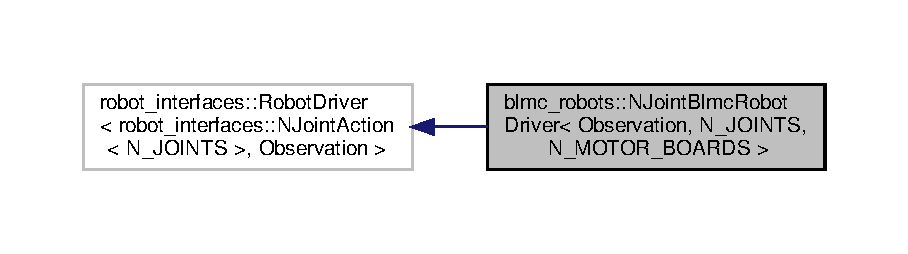
\includegraphics[width=350pt]{classblmc__robots_1_1NJointBlmcRobotDriver__inherit__graph}
\end{center}
\end{figure}


Collaboration diagram for blmc\+\_\+robots\+:\+:N\+Joint\+Blmc\+Robot\+Driver$<$ Observation, N\+\_\+\+J\+O\+I\+N\+TS, N\+\_\+\+M\+O\+T\+O\+R\+\_\+\+B\+O\+A\+R\+DS $>$\+:
\nopagebreak
\begin{figure}[H]
\begin{center}
\leavevmode
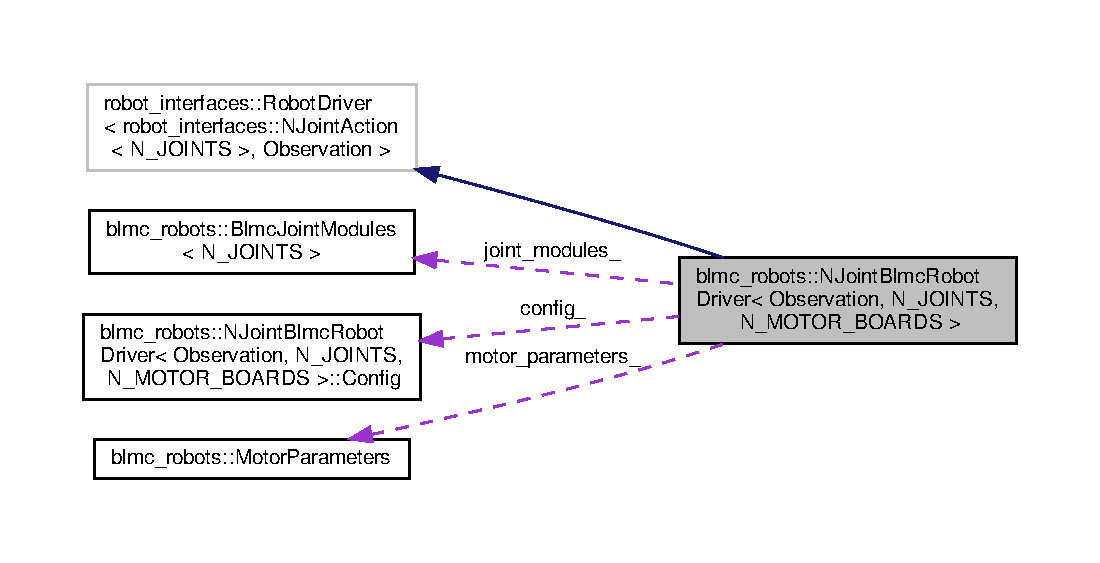
\includegraphics[width=350pt]{classblmc__robots_1_1NJointBlmcRobotDriver__coll__graph}
\end{center}
\end{figure}
\subsection*{Classes}
\begin{DoxyCompactItemize}
\item 
struct \hyperlink{structblmc__robots_1_1NJointBlmcRobotDriver_1_1Config}{Config}
\begin{DoxyCompactList}\small\item\em Configuration of the robot that can be changed by the user. \end{DoxyCompactList}\end{DoxyCompactItemize}
\subsection*{Public Types}
\begin{DoxyCompactItemize}
\item 
\mbox{\Hypertarget{classblmc__robots_1_1NJointBlmcRobotDriver_a6c04fde05f933db1703457f94c6cef6b}\label{classblmc__robots_1_1NJointBlmcRobotDriver_a6c04fde05f933db1703457f94c6cef6b}} 
typedef robot\+\_\+interfaces\+::\+N\+Joint\+Action$<$ N\+\_\+\+J\+O\+I\+N\+TS $>$ {\bfseries Action}
\item 
\mbox{\Hypertarget{classblmc__robots_1_1NJointBlmcRobotDriver_a4827e39990852c1743ce095a74213ac0}\label{classblmc__robots_1_1NJointBlmcRobotDriver_a4827e39990852c1743ce095a74213ac0}} 
typedef robot\+\_\+interfaces\+::\+Robot\+Interface\+Types$<$ Action, Observation $>$ {\bfseries Types}
\item 
\mbox{\Hypertarget{classblmc__robots_1_1NJointBlmcRobotDriver_acdeabef6dc3a084af61da9eda3555083}\label{classblmc__robots_1_1NJointBlmcRobotDriver_acdeabef6dc3a084af61da9eda3555083}} 
typedef Action\+::\+Vector {\bfseries Vector}
\item 
\mbox{\Hypertarget{classblmc__robots_1_1NJointBlmcRobotDriver_a38bce1426a7ad5418dff1d43d0fc338e}\label{classblmc__robots_1_1NJointBlmcRobotDriver_a38bce1426a7ad5418dff1d43d0fc338e}} 
typedef std\+::array$<$ std\+::shared\+\_\+ptr$<$ blmc\+\_\+drivers\+::\+Motor\+Interface $>$, N\+\_\+\+J\+O\+I\+N\+TS $>$ {\bfseries Motors}
\item 
\mbox{\Hypertarget{classblmc__robots_1_1NJointBlmcRobotDriver_ab703f92d3c01fbd3d481f886bfb81eca}\label{classblmc__robots_1_1NJointBlmcRobotDriver_ab703f92d3c01fbd3d481f886bfb81eca}} 
typedef std\+::array$<$ std\+::shared\+\_\+ptr$<$ blmc\+\_\+drivers\+::\+Can\+Bus\+Motor\+Board $>$, N\+\_\+\+M\+O\+T\+O\+R\+\_\+\+B\+O\+A\+R\+DS $>$ {\bfseries Motor\+Boards}
\end{DoxyCompactItemize}
\subsection*{Public Member Functions}
\begin{DoxyCompactItemize}
\item 
\mbox{\Hypertarget{classblmc__robots_1_1NJointBlmcRobotDriver_acc2af471c4db682f57854d14430ef3fa}\label{classblmc__robots_1_1NJointBlmcRobotDriver_acc2af471c4db682f57854d14430ef3fa}} 
{\bfseries N\+Joint\+Blmc\+Robot\+Driver} (const Motor\+Boards \&motor\+\_\+boards, const Motors \&motors, const \hyperlink{structblmc__robots_1_1MotorParameters}{Motor\+Parameters} \&motor\+\_\+parameters, const \hyperlink{structblmc__robots_1_1NJointBlmcRobotDriver_1_1Config}{Config} \&config)
\item 
\mbox{\Hypertarget{classblmc__robots_1_1NJointBlmcRobotDriver_a8bfdae3670c639a7dc129e17687b0285}\label{classblmc__robots_1_1NJointBlmcRobotDriver_a8bfdae3670c639a7dc129e17687b0285}} 
Vector {\bfseries get\+\_\+max\+\_\+torques} () const
\item 
\mbox{\Hypertarget{classblmc__robots_1_1NJointBlmcRobotDriver_a9ac3d22be40ce2c6f8bafd901bdb4a3d}\label{classblmc__robots_1_1NJointBlmcRobotDriver_a9ac3d22be40ce2c6f8bafd901bdb4a3d}} 
void {\bfseries pause\+\_\+motors} ()
\item 
\mbox{\Hypertarget{classblmc__robots_1_1NJointBlmcRobotDriver_a274d4d97156b77e6f2dcfda74d67e45c}\label{classblmc__robots_1_1NJointBlmcRobotDriver_a274d4d97156b77e6f2dcfda74d67e45c}} 
Vector {\bfseries get\+\_\+measured\+\_\+index\+\_\+angles} () const
\item 
void \hyperlink{classblmc__robots_1_1NJointBlmcRobotDriver_a7a1ece2b5d4f0f607a4d0516543b0d48}{initialize} () override
\begin{DoxyCompactList}\small\item\em Find home position of all joints and move to start position. \end{DoxyCompactList}\item 
\mbox{\Hypertarget{classblmc__robots_1_1NJointBlmcRobotDriver_abc4c63313e05020b91dad26a580e184f}\label{classblmc__robots_1_1NJointBlmcRobotDriver_abc4c63313e05020b91dad26a580e184f}} 
virtual Observation {\bfseries get\+\_\+latest\+\_\+observation} () override=0
\item 
\mbox{\Hypertarget{classblmc__robots_1_1NJointBlmcRobotDriver_a200a5a050a1e2d493f47dc1228319d27}\label{classblmc__robots_1_1NJointBlmcRobotDriver_a200a5a050a1e2d493f47dc1228319d27}} 
Action {\bfseries apply\+\_\+action} (const Action \&desired\+\_\+action) override
\item 
\mbox{\Hypertarget{classblmc__robots_1_1NJointBlmcRobotDriver_a2c45384d83e688618a589cb13797e3bc}\label{classblmc__robots_1_1NJointBlmcRobotDriver_a2c45384d83e688618a589cb13797e3bc}} 
std\+::string {\bfseries get\+\_\+error} () override
\item 
\mbox{\Hypertarget{classblmc__robots_1_1NJointBlmcRobotDriver_a4d57e567a2cd393ee9e4af4bcdde94f0}\label{classblmc__robots_1_1NJointBlmcRobotDriver_a4d57e567a2cd393ee9e4af4bcdde94f0}} 
void {\bfseries shutdown} () override
\item 
bool \hyperlink{classblmc__robots_1_1NJointBlmcRobotDriver_a1d9aedee4887a6f34c07481c4520cb5a}{is\+\_\+within\+\_\+hard\+\_\+position\+\_\+limits} (const Observation \&observation) const
\begin{DoxyCompactList}\small\item\em Check if the joint position is within the hard limits. \end{DoxyCompactList}\end{DoxyCompactItemize}
\subsection*{Static Public Member Functions}
\begin{DoxyCompactItemize}
\item 
\mbox{\Hypertarget{classblmc__robots_1_1NJointBlmcRobotDriver_a30f5a6037441bff26ab208bbb91c0c39}\label{classblmc__robots_1_1NJointBlmcRobotDriver_a30f5a6037441bff26ab208bbb91c0c39}} 
static Motor\+Boards {\bfseries create\+\_\+motor\+\_\+boards} (const std\+::array$<$ std\+::string, N\+\_\+\+M\+O\+T\+O\+R\+\_\+\+B\+O\+A\+R\+DS $>$ \&can\+\_\+ports)
\item 
static Action \hyperlink{classblmc__robots_1_1NJointBlmcRobotDriver_a8f7aaf3bc10c0d4d0f2c7a38f594c166}{process\+\_\+desired\+\_\+action} (const Action \&desired\+\_\+action, const Observation \&latest\+\_\+observation, const double max\+\_\+torque\+\_\+\+Nm, const Vector \&safety\+\_\+kd, const Vector \&default\+\_\+position\+\_\+control\+\_\+kp, const Vector \&default\+\_\+position\+\_\+control\+\_\+kd, const Vector \&lower\+\_\+position\+\_\+limits=Vector\+::\+Constant(-\/std\+::numeric\+\_\+limits$<$ double $>$\+::infinity()), const Vector \&upper\+\_\+position\+\_\+limits=Vector\+::\+Constant(std\+::numeric\+\_\+limits$<$ double $>$\+::infinity()))
\begin{DoxyCompactList}\small\item\em Process the desired action provided by the user. \end{DoxyCompactList}\end{DoxyCompactItemize}
\subsection*{Public Attributes}
\begin{DoxyCompactItemize}
\item 
const bool \hyperlink{classblmc__robots_1_1NJointBlmcRobotDriver_a584b85a9e8356e4afcdf1559edd700cc}{has\+\_\+endstop\+\_\+}
\begin{DoxyCompactList}\small\item\em True if the joints have mechanical end stops, false if not. \end{DoxyCompactList}\end{DoxyCompactItemize}
\subsection*{Static Public Attributes}
\begin{DoxyCompactItemize}
\item 
\mbox{\Hypertarget{classblmc__robots_1_1NJointBlmcRobotDriver_a933b81d922085d51a8138cbb648c3e64}\label{classblmc__robots_1_1NJointBlmcRobotDriver_a933b81d922085d51a8138cbb648c3e64}} 
static constexpr size\+\_\+t {\bfseries num\+\_\+joints} = N\+\_\+\+J\+O\+I\+N\+TS
\item 
\mbox{\Hypertarget{classblmc__robots_1_1NJointBlmcRobotDriver_ad4897dda6376b6fabdf4b5ecd43c6c4c}\label{classblmc__robots_1_1NJointBlmcRobotDriver_ad4897dda6376b6fabdf4b5ecd43c6c4c}} 
static constexpr size\+\_\+t {\bfseries num\+\_\+motor\+\_\+boards} = N\+\_\+\+M\+O\+T\+O\+R\+\_\+\+B\+O\+A\+R\+DS
\end{DoxyCompactItemize}
\subsection*{Protected Member Functions}
\begin{DoxyCompactItemize}
\item 
\mbox{\Hypertarget{classblmc__robots_1_1NJointBlmcRobotDriver_aeca6dbdd22e3b40afe89fecf2895dcad}\label{classblmc__robots_1_1NJointBlmcRobotDriver_aeca6dbdd22e3b40afe89fecf2895dcad}} 
Action {\bfseries apply\+\_\+action\+\_\+uninitialized} (const Action \&desired\+\_\+action)
\item 
void \hyperlink{classblmc__robots_1_1NJointBlmcRobotDriver_aafa20130f746b5cc35eae43ce36e23c6}{\+\_\+initialize} ()
\begin{DoxyCompactList}\small\item\em Actual initialization that is called in a real-\/time thread in \hyperlink{classblmc__robots_1_1NJointBlmcRobotDriver_a7a1ece2b5d4f0f607a4d0516543b0d48}{initialize()}. \end{DoxyCompactList}\item 
bool \hyperlink{classblmc__robots_1_1NJointBlmcRobotDriver_aa2948efef69215afb233fc63acf88d3f}{homing} (Vector \hyperlink{n__joint__blmc__robot__driver_8hpp_a8f0c3d2c5211dc9fd38c4d64bdcf77cb}{endstop\+\_\+search\+\_\+torques\+\_\+\+Nm}, Vector home\+\_\+offset\+\_\+rad=Vector\+::\+Zero())
\begin{DoxyCompactList}\small\item\em Homing using end stops (optional) and encoder indices. \end{DoxyCompactList}\item 
bool \hyperlink{classblmc__robots_1_1NJointBlmcRobotDriver_ab29cab22a765bce463f367b6e6dc82ff}{move\+\_\+to\+\_\+position} (const Vector \&goal\+\_\+pos, const double tolerance, const uint32\+\_\+t time\+\_\+steps)
\begin{DoxyCompactList}\small\item\em Move to given goal position with a minimum jerk trajectory. \end{DoxyCompactList}\end{DoxyCompactItemize}
\subsection*{Protected Attributes}
\begin{DoxyCompactItemize}
\item 
\mbox{\Hypertarget{classblmc__robots_1_1NJointBlmcRobotDriver_a17f32687708f95c1160ecb708d429ccd}\label{classblmc__robots_1_1NJointBlmcRobotDriver_a17f32687708f95c1160ecb708d429ccd}} 
\hyperlink{classblmc__robots_1_1BlmcJointModules}{Blmc\+Joint\+Modules}$<$ N\+\_\+\+J\+O\+I\+N\+TS $>$ {\bfseries joint\+\_\+modules\+\_\+}
\item 
\mbox{\Hypertarget{classblmc__robots_1_1NJointBlmcRobotDriver_ad760af5444951e4ce505e45b4e13d4ca}\label{classblmc__robots_1_1NJointBlmcRobotDriver_ad760af5444951e4ce505e45b4e13d4ca}} 
Motor\+Boards {\bfseries motor\+\_\+boards\+\_\+}
\item 
\mbox{\Hypertarget{classblmc__robots_1_1NJointBlmcRobotDriver_ad5e1875908bb62b2f014c3f8dfce969d}\label{classblmc__robots_1_1NJointBlmcRobotDriver_ad5e1875908bb62b2f014c3f8dfce969d}} 
\hyperlink{structblmc__robots_1_1MotorParameters}{Motor\+Parameters} \hyperlink{classblmc__robots_1_1NJointBlmcRobotDriver_ad5e1875908bb62b2f014c3f8dfce969d}{motor\+\_\+parameters\+\_\+}
\begin{DoxyCompactList}\small\item\em Fixed motor parameters (assuming all joints use same setup). \end{DoxyCompactList}\item 
\mbox{\Hypertarget{classblmc__robots_1_1NJointBlmcRobotDriver_a62f708a1406f8dfb68361c5698a5559b}\label{classblmc__robots_1_1NJointBlmcRobotDriver_a62f708a1406f8dfb68361c5698a5559b}} 
double \hyperlink{classblmc__robots_1_1NJointBlmcRobotDriver_a62f708a1406f8dfb68361c5698a5559b}{max\+\_\+torque\+\_\+\+Nm\+\_\+}
\begin{DoxyCompactList}\small\item\em Maximum torque allowed on each joint. \end{DoxyCompactList}\item 
\hyperlink{structblmc__robots_1_1NJointBlmcRobotDriver_1_1Config}{Config} \hyperlink{classblmc__robots_1_1NJointBlmcRobotDriver_a5af27a320384e0189725ee1b13edc314}{config\+\_\+}
\begin{DoxyCompactList}\small\item\em User-\/defined configuration of the driver. \end{DoxyCompactList}\item 
\mbox{\Hypertarget{classblmc__robots_1_1NJointBlmcRobotDriver_af11037c8c3395fcde191037c82ba6c0a}\label{classblmc__robots_1_1NJointBlmcRobotDriver_af11037c8c3395fcde191037c82ba6c0a}} 
bool {\bfseries is\+\_\+initialized\+\_\+} = false
\end{DoxyCompactItemize}


\subsection{Detailed Description}
\subsubsection*{template$<$typename Observation, size\+\_\+t N\+\_\+\+J\+O\+I\+N\+TS, size\+\_\+t N\+\_\+\+M\+O\+T\+O\+R\+\_\+\+B\+O\+A\+R\+DS$>$\newline
class blmc\+\_\+robots\+::\+N\+Joint\+Blmc\+Robot\+Driver$<$ Observation, N\+\_\+\+J\+O\+I\+N\+T\+S, N\+\_\+\+M\+O\+T\+O\+R\+\_\+\+B\+O\+A\+R\+D\+S $>$}

Base class for n-\/joint B\+L\+MC robots. 

This is a generic base class to easily implement drivers for simple B\+L\+MC robots that consist of N\+\_\+\+J\+O\+I\+N\+TS joints.


\begin{DoxyTemplParams}{Template Parameters}
{\em N\+\_\+\+J\+O\+I\+N\+TS} & Number of joints. \\
\hline
{\em N\+\_\+\+M\+O\+T\+O\+R\+\_\+\+B\+O\+A\+R\+DS} & Number of motor control boards that are used. \\
\hline
\end{DoxyTemplParams}


\subsection{Member Function Documentation}
\mbox{\Hypertarget{classblmc__robots_1_1NJointBlmcRobotDriver_aafa20130f746b5cc35eae43ce36e23c6}\label{classblmc__robots_1_1NJointBlmcRobotDriver_aafa20130f746b5cc35eae43ce36e23c6}} 
\index{blmc\+\_\+robots\+::\+N\+Joint\+Blmc\+Robot\+Driver@{blmc\+\_\+robots\+::\+N\+Joint\+Blmc\+Robot\+Driver}!\+\_\+initialize@{\+\_\+initialize}}
\index{\+\_\+initialize@{\+\_\+initialize}!blmc\+\_\+robots\+::\+N\+Joint\+Blmc\+Robot\+Driver@{blmc\+\_\+robots\+::\+N\+Joint\+Blmc\+Robot\+Driver}}
\subsubsection{\texorpdfstring{\+\_\+initialize()}{\_initialize()}}
{\footnotesize\ttfamily template$<$typename Observation, size\+\_\+t N\+\_\+\+J\+O\+I\+N\+TS, size\+\_\+t N\+\_\+\+M\+O\+T\+O\+R\+\_\+\+B\+O\+A\+R\+DS$>$ \\
void \hyperlink{classblmc__robots_1_1NJointBlmcRobotDriver}{blmc\+\_\+robots\+::\+N\+Joint\+Blmc\+Robot\+Driver}$<$ Observation, N\+\_\+\+J\+O\+I\+N\+TS, N\+\_\+\+M\+O\+T\+O\+R\+\_\+\+B\+O\+A\+R\+DS $>$\+::\+\_\+initialize (\begin{DoxyParamCaption}{ }\end{DoxyParamCaption})\hspace{0.3cm}{\ttfamily [protected]}}



Actual initialization that is called in a real-\/time thread in \hyperlink{classblmc__robots_1_1NJointBlmcRobotDriver_a7a1ece2b5d4f0f607a4d0516543b0d48}{initialize()}. 

\mbox{\Hypertarget{classblmc__robots_1_1NJointBlmcRobotDriver_aa2948efef69215afb233fc63acf88d3f}\label{classblmc__robots_1_1NJointBlmcRobotDriver_aa2948efef69215afb233fc63acf88d3f}} 
\index{blmc\+\_\+robots\+::\+N\+Joint\+Blmc\+Robot\+Driver@{blmc\+\_\+robots\+::\+N\+Joint\+Blmc\+Robot\+Driver}!homing@{homing}}
\index{homing@{homing}!blmc\+\_\+robots\+::\+N\+Joint\+Blmc\+Robot\+Driver@{blmc\+\_\+robots\+::\+N\+Joint\+Blmc\+Robot\+Driver}}
\subsubsection{\texorpdfstring{homing()}{homing()}}
{\footnotesize\ttfamily template$<$typename Observation, size\+\_\+t N\+\_\+\+J\+O\+I\+N\+TS, size\+\_\+t N\+\_\+\+M\+O\+T\+O\+R\+\_\+\+B\+O\+A\+R\+DS$>$ \\
bool \hyperlink{classblmc__robots_1_1NJointBlmcRobotDriver}{blmc\+\_\+robots\+::\+N\+Joint\+Blmc\+Robot\+Driver}$<$ Observation, N\+\_\+\+J\+O\+I\+N\+TS, N\+\_\+\+M\+O\+T\+O\+R\+\_\+\+B\+O\+A\+R\+DS $>$\+::homing (\begin{DoxyParamCaption}\item[{Vector}]{endstop\+\_\+search\+\_\+torques\+\_\+\+Nm,  }\item[{Vector}]{home\+\_\+offset\+\_\+rad = {\ttfamily Vector\+:\+:Zero()} }\end{DoxyParamCaption})\hspace{0.3cm}{\ttfamily [protected]}}



Homing using end stops (optional) and encoder indices. 

Procedure for finding an absolute zero position (or \char`\"{}home\char`\"{} position) when using relative encoders.

If the robot has end stops (according to configuration), all joints first move in negative direction until they hit the end stop. Then an encoder index search is started where each joint moves slowly in positive direction until the next encoder index. The position of this encoder index is the \char`\"{}home position\char`\"{}.

By default, the zero position is the same as the home position. The optional argument home\+\_\+offset\+\_\+rad provides a means to move the zero position relative to the home position. The zero position is computed as \begin{DoxyVerb}zero position = encoder index position + home offset
\end{DoxyVerb}



\begin{DoxyParams}{Parameters}
{\em endstop\+\_\+search\+\_\+torques\+\_\+\+Nm} & Torques that are used to move the joints while searching the end stop. \\
\hline
{\em home\+\_\+offset\+\_\+rad} & Offset between the home position and the desired zero position. \\
\hline
\end{DoxyParams}
\mbox{\Hypertarget{classblmc__robots_1_1NJointBlmcRobotDriver_a7a1ece2b5d4f0f607a4d0516543b0d48}\label{classblmc__robots_1_1NJointBlmcRobotDriver_a7a1ece2b5d4f0f607a4d0516543b0d48}} 
\index{blmc\+\_\+robots\+::\+N\+Joint\+Blmc\+Robot\+Driver@{blmc\+\_\+robots\+::\+N\+Joint\+Blmc\+Robot\+Driver}!initialize@{initialize}}
\index{initialize@{initialize}!blmc\+\_\+robots\+::\+N\+Joint\+Blmc\+Robot\+Driver@{blmc\+\_\+robots\+::\+N\+Joint\+Blmc\+Robot\+Driver}}
\subsubsection{\texorpdfstring{initialize()}{initialize()}}
{\footnotesize\ttfamily template$<$typename Observation, size\+\_\+t N\+\_\+\+J\+O\+I\+N\+TS, size\+\_\+t N\+\_\+\+M\+O\+T\+O\+R\+\_\+\+B\+O\+A\+R\+DS$>$ \\
void \hyperlink{classblmc__robots_1_1NJointBlmcRobotDriver}{blmc\+\_\+robots\+::\+N\+Joint\+Blmc\+Robot\+Driver}$<$ Observation, N\+\_\+\+J\+O\+I\+N\+TS, N\+\_\+\+M\+O\+T\+O\+R\+\_\+\+B\+O\+A\+R\+DS $>$\+::initialize (\begin{DoxyParamCaption}{ }\end{DoxyParamCaption})\hspace{0.3cm}{\ttfamily [override]}}



Find home position of all joints and move to start position. 

Homes all joints using home\+\_\+on\+\_\+index\+\_\+after\+\_\+negative\+\_\+end\+\_\+stop. When finished, move the joint to the starting position (defined in {\ttfamily config\+\_\+.\+initial\+\_\+position\+\_\+rad}). \mbox{\Hypertarget{classblmc__robots_1_1NJointBlmcRobotDriver_a1d9aedee4887a6f34c07481c4520cb5a}\label{classblmc__robots_1_1NJointBlmcRobotDriver_a1d9aedee4887a6f34c07481c4520cb5a}} 
\index{blmc\+\_\+robots\+::\+N\+Joint\+Blmc\+Robot\+Driver@{blmc\+\_\+robots\+::\+N\+Joint\+Blmc\+Robot\+Driver}!is\+\_\+within\+\_\+hard\+\_\+position\+\_\+limits@{is\+\_\+within\+\_\+hard\+\_\+position\+\_\+limits}}
\index{is\+\_\+within\+\_\+hard\+\_\+position\+\_\+limits@{is\+\_\+within\+\_\+hard\+\_\+position\+\_\+limits}!blmc\+\_\+robots\+::\+N\+Joint\+Blmc\+Robot\+Driver@{blmc\+\_\+robots\+::\+N\+Joint\+Blmc\+Robot\+Driver}}
\subsubsection{\texorpdfstring{is\+\_\+within\+\_\+hard\+\_\+position\+\_\+limits()}{is\_within\_hard\_position\_limits()}}
{\footnotesize\ttfamily template$<$typename Observation, size\+\_\+t N\+\_\+\+J\+O\+I\+N\+TS, size\+\_\+t N\+\_\+\+M\+O\+T\+O\+R\+\_\+\+B\+O\+A\+R\+DS$>$ \\
bool \hyperlink{classblmc__robots_1_1NJointBlmcRobotDriver}{blmc\+\_\+robots\+::\+N\+Joint\+Blmc\+Robot\+Driver}$<$ Observation, N\+\_\+\+J\+O\+I\+N\+TS, N\+\_\+\+M\+O\+T\+O\+R\+\_\+\+B\+O\+A\+R\+DS $>$\+::is\+\_\+within\+\_\+hard\+\_\+position\+\_\+limits (\begin{DoxyParamCaption}\item[{const Observation \&}]{observation }\end{DoxyParamCaption}) const}



Check if the joint position is within the hard limits. 

\begin{DoxySeeAlso}{See also}
\hyperlink{structblmc__robots_1_1NJointBlmcRobotDriver_1_1Config_ae34fb8f28bdec0401b72b09bc8d48b65}{Config\+::is\+\_\+within\+\_\+hard\+\_\+position\+\_\+limits} 
\end{DoxySeeAlso}
\mbox{\Hypertarget{classblmc__robots_1_1NJointBlmcRobotDriver_ab29cab22a765bce463f367b6e6dc82ff}\label{classblmc__robots_1_1NJointBlmcRobotDriver_ab29cab22a765bce463f367b6e6dc82ff}} 
\index{blmc\+\_\+robots\+::\+N\+Joint\+Blmc\+Robot\+Driver@{blmc\+\_\+robots\+::\+N\+Joint\+Blmc\+Robot\+Driver}!move\+\_\+to\+\_\+position@{move\+\_\+to\+\_\+position}}
\index{move\+\_\+to\+\_\+position@{move\+\_\+to\+\_\+position}!blmc\+\_\+robots\+::\+N\+Joint\+Blmc\+Robot\+Driver@{blmc\+\_\+robots\+::\+N\+Joint\+Blmc\+Robot\+Driver}}
\subsubsection{\texorpdfstring{move\+\_\+to\+\_\+position()}{move\_to\_position()}}
{\footnotesize\ttfamily template$<$typename Observation, size\+\_\+t N\+\_\+\+J\+O\+I\+N\+TS, size\+\_\+t N\+\_\+\+M\+O\+T\+O\+R\+\_\+\+B\+O\+A\+R\+DS$>$ \\
bool \hyperlink{classblmc__robots_1_1NJointBlmcRobotDriver}{blmc\+\_\+robots\+::\+N\+Joint\+Blmc\+Robot\+Driver}$<$ Observation, N\+\_\+\+J\+O\+I\+N\+TS, N\+\_\+\+M\+O\+T\+O\+R\+\_\+\+B\+O\+A\+R\+DS $>$\+::move\+\_\+to\+\_\+position (\begin{DoxyParamCaption}\item[{const Vector \&}]{goal\+\_\+pos,  }\item[{const double}]{tolerance,  }\item[{const uint32\+\_\+t}]{time\+\_\+steps }\end{DoxyParamCaption})\hspace{0.3cm}{\ttfamily [protected]}}



Move to given goal position with a minimum jerk trajectory. 

Use a series of position actions to move to the given goal position on a minimum jerk trajectory.


\begin{DoxyParams}{Parameters}
{\em goal\+\_\+pos} & Angular goal position for each joint. \\
\hline
{\em tolerance} & Allowed position error for reaching the goal. This is checked per joint, that is the maximal possible error is +/-\/tolerance on each joint. \\
\hline
{\em time\+\_\+steps} & Number of control loop cycles for reaching the goal. The lower the number of steps, the faster the robot will move. \\
\hline
\end{DoxyParams}
\begin{DoxyReturn}{Returns}
True if goal position is reached, false if timeout is exceeded. 
\end{DoxyReturn}
\mbox{\Hypertarget{classblmc__robots_1_1NJointBlmcRobotDriver_a8f7aaf3bc10c0d4d0f2c7a38f594c166}\label{classblmc__robots_1_1NJointBlmcRobotDriver_a8f7aaf3bc10c0d4d0f2c7a38f594c166}} 
\index{blmc\+\_\+robots\+::\+N\+Joint\+Blmc\+Robot\+Driver@{blmc\+\_\+robots\+::\+N\+Joint\+Blmc\+Robot\+Driver}!process\+\_\+desired\+\_\+action@{process\+\_\+desired\+\_\+action}}
\index{process\+\_\+desired\+\_\+action@{process\+\_\+desired\+\_\+action}!blmc\+\_\+robots\+::\+N\+Joint\+Blmc\+Robot\+Driver@{blmc\+\_\+robots\+::\+N\+Joint\+Blmc\+Robot\+Driver}}
\subsubsection{\texorpdfstring{process\+\_\+desired\+\_\+action()}{process\_desired\_action()}}
{\footnotesize\ttfamily template$<$typename Observation, size\+\_\+t N\+\_\+\+J\+O\+I\+N\+TS, size\+\_\+t N\+\_\+\+M\+O\+T\+O\+R\+\_\+\+B\+O\+A\+R\+DS$>$ \\
static Action \hyperlink{classblmc__robots_1_1NJointBlmcRobotDriver}{blmc\+\_\+robots\+::\+N\+Joint\+Blmc\+Robot\+Driver}$<$ Observation, N\+\_\+\+J\+O\+I\+N\+TS, N\+\_\+\+M\+O\+T\+O\+R\+\_\+\+B\+O\+A\+R\+DS $>$\+::process\+\_\+desired\+\_\+action (\begin{DoxyParamCaption}\item[{const Action \&}]{desired\+\_\+action,  }\item[{const Observation \&}]{latest\+\_\+observation,  }\item[{const double}]{max\+\_\+torque\+\_\+\+Nm,  }\item[{const Vector \&}]{safety\+\_\+kd,  }\item[{const Vector \&}]{default\+\_\+position\+\_\+control\+\_\+kp,  }\item[{const Vector \&}]{default\+\_\+position\+\_\+control\+\_\+kd,  }\item[{const Vector \&}]{lower\+\_\+position\+\_\+limits = {\ttfamily Vector\+:\+:Constant(-\/std\+:\+:numeric\+\_\+limits$<$~double~$>$\+:\+:infinity())},  }\item[{const Vector \&}]{upper\+\_\+position\+\_\+limits = {\ttfamily Vector\+:\+:Constant(std\+:\+:numeric\+\_\+limits$<$~double~$>$\+:\+:infinity())} }\end{DoxyParamCaption})\hspace{0.3cm}{\ttfamily [static]}}



Process the desired action provided by the user. 

Takes the desired action from the user and does the following processing\+:

\subsubsection*{1. Check position limits}

If the observed position of a joint exceeds the limits, actions for that joint that do not point back towards the allowed range are replaced with a position command to the limit value. Further custom P\+D-\/gains are ignored in this case.

\subsubsection*{2. Run the position controller in case a target position is set.}

If the target position is set to a value unequal to NaN for any joint, a PD position controller is executed for this joint and the resulting torque command is added to the torque command in the action.

If the P-\/ and/or D-\/gains are set to a non-\/\+NaN value in the action, they are used for the control. Na\+N-\/values are replaced with the default gains.

\subsubsection*{3. Apply safety checks.}


\begin{DoxyItemize}
\item Limit the torque to the allowed maximum value.
\item Dampen velocity using the given safety\+\_\+kd gains. Damping us done joint-\/wise using this equation\+: \begin{DoxyVerb}torque_damped = torque_desired - safety_kd * current_velocity
\end{DoxyVerb}

\end{DoxyItemize}

The resulting action with modifications of all steps is returned.


\begin{DoxyParams}{Parameters}
{\em desired\+\_\+action} & Desired action given by the user. \\
\hline
{\em latest\+\_\+observation} & Latest observation from the robot. \\
\hline
{\em max\+\_\+torque\+\_\+\+Nm} & Maximum allowed absolute torque. \\
\hline
{\em safety\+\_\+kd} & D-\/gain for velocity damping. \\
\hline
{\em default\+\_\+position\+\_\+control\+\_\+kp} & Default P-\/gain for position control. \\
\hline
{\em default\+\_\+position\+\_\+control\+\_\+kd} & Default D-\/gain for position control. \\
\hline
{\em lower\+\_\+position\+\_\+limits} & Lower limits for joint positions. \\
\hline
{\em upper\+\_\+position\+\_\+limits} & Upper limits for joint positions.\\
\hline
\end{DoxyParams}
\begin{DoxyReturn}{Returns}
Resulting action after applying all the processing. 
\end{DoxyReturn}


\subsection{Member Data Documentation}
\mbox{\Hypertarget{classblmc__robots_1_1NJointBlmcRobotDriver_a5af27a320384e0189725ee1b13edc314}\label{classblmc__robots_1_1NJointBlmcRobotDriver_a5af27a320384e0189725ee1b13edc314}} 
\index{blmc\+\_\+robots\+::\+N\+Joint\+Blmc\+Robot\+Driver@{blmc\+\_\+robots\+::\+N\+Joint\+Blmc\+Robot\+Driver}!config\+\_\+@{config\+\_\+}}
\index{config\+\_\+@{config\+\_\+}!blmc\+\_\+robots\+::\+N\+Joint\+Blmc\+Robot\+Driver@{blmc\+\_\+robots\+::\+N\+Joint\+Blmc\+Robot\+Driver}}
\subsubsection{\texorpdfstring{config\+\_\+}{config\_}}
{\footnotesize\ttfamily template$<$typename Observation, size\+\_\+t N\+\_\+\+J\+O\+I\+N\+TS, size\+\_\+t N\+\_\+\+M\+O\+T\+O\+R\+\_\+\+B\+O\+A\+R\+DS$>$ \\
\hyperlink{structblmc__robots_1_1NJointBlmcRobotDriver_1_1Config}{Config} \hyperlink{classblmc__robots_1_1NJointBlmcRobotDriver}{blmc\+\_\+robots\+::\+N\+Joint\+Blmc\+Robot\+Driver}$<$ Observation, N\+\_\+\+J\+O\+I\+N\+TS, N\+\_\+\+M\+O\+T\+O\+R\+\_\+\+B\+O\+A\+R\+DS $>$\+::config\+\_\+\hspace{0.3cm}{\ttfamily [protected]}}



User-\/defined configuration of the driver. 

Contains all configuration values that can be modified by the user (via the configuration file). \mbox{\Hypertarget{classblmc__robots_1_1NJointBlmcRobotDriver_a584b85a9e8356e4afcdf1559edd700cc}\label{classblmc__robots_1_1NJointBlmcRobotDriver_a584b85a9e8356e4afcdf1559edd700cc}} 
\index{blmc\+\_\+robots\+::\+N\+Joint\+Blmc\+Robot\+Driver@{blmc\+\_\+robots\+::\+N\+Joint\+Blmc\+Robot\+Driver}!has\+\_\+endstop\+\_\+@{has\+\_\+endstop\+\_\+}}
\index{has\+\_\+endstop\+\_\+@{has\+\_\+endstop\+\_\+}!blmc\+\_\+robots\+::\+N\+Joint\+Blmc\+Robot\+Driver@{blmc\+\_\+robots\+::\+N\+Joint\+Blmc\+Robot\+Driver}}
\subsubsection{\texorpdfstring{has\+\_\+endstop\+\_\+}{has\_endstop\_}}
{\footnotesize\ttfamily template$<$typename Observation, size\+\_\+t N\+\_\+\+J\+O\+I\+N\+TS, size\+\_\+t N\+\_\+\+M\+O\+T\+O\+R\+\_\+\+B\+O\+A\+R\+DS$>$ \\
const bool \hyperlink{classblmc__robots_1_1NJointBlmcRobotDriver}{blmc\+\_\+robots\+::\+N\+Joint\+Blmc\+Robot\+Driver}$<$ Observation, N\+\_\+\+J\+O\+I\+N\+TS, N\+\_\+\+M\+O\+T\+O\+R\+\_\+\+B\+O\+A\+R\+DS $>$\+::has\+\_\+endstop\+\_\+}



True if the joints have mechanical end stops, false if not. 

If set to true, it is assumed that all joints of the robot have end stops that mechanically prevent them from moving out of the valid range.

If present, the end stops are used for a fully automated homing procedure in which the joints first move until they hit the end stop before starting the encoder index search. This way it is ensured that the correct index is used for homing without any need for manual set up. 

The documentation for this class was generated from the following file\+:\begin{DoxyCompactItemize}
\item 
include/blmc\+\_\+robots/\hyperlink{n__joint__blmc__robot__driver_8hpp}{n\+\_\+joint\+\_\+blmc\+\_\+robot\+\_\+driver.\+hpp}\end{DoxyCompactItemize}

\hypertarget{classblmc__robots_1_1Polynome}{}\section{blmc\+\_\+robots\+:\+:Polynome$<$ O\+R\+D\+ER $>$ Class Template Reference}
\label{classblmc__robots_1_1Polynome}\index{blmc\+\_\+robots\+::\+Polynome$<$ O\+R\+D\+E\+R $>$@{blmc\+\_\+robots\+::\+Polynome$<$ O\+R\+D\+E\+R $>$}}


Simple class that defines $ P(x) $ a polynome of order O\+R\+D\+ER.  




{\ttfamily \#include $<$polynome.\+hpp$>$}



Inheritance diagram for blmc\+\_\+robots\+:\+:Polynome$<$ O\+R\+D\+ER $>$\+:
\nopagebreak
\begin{figure}[H]
\begin{center}
\leavevmode
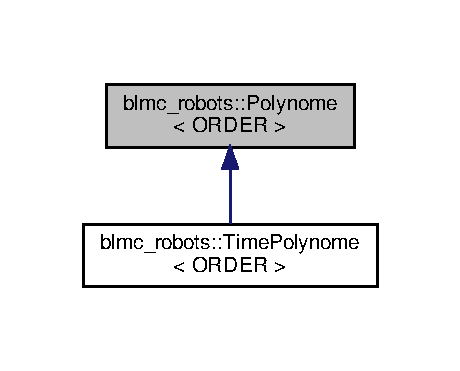
\includegraphics[width=221pt]{classblmc__robots_1_1Polynome__inherit__graph}
\end{center}
\end{figure}
\subsection*{Public Member Functions}
\begin{DoxyCompactItemize}
\item 
\hyperlink{classblmc__robots_1_1Polynome_a8ece7a7021cc62167c023d51a5bb3879}{Polynome} ()
\begin{DoxyCompactList}\small\item\em Polynome$<$\+O\+R\+D\+E\+R$>$ definitions. \end{DoxyCompactList}\item 
\hyperlink{classblmc__robots_1_1Polynome_a4541e4b629061dfdbca73559a42a6e93}{$\sim$\+Polynome} ()
\item 
double \hyperlink{classblmc__robots_1_1Polynome_ae102191e0f730744e822c8e7599008d6}{compute} (double x)
\item 
double \hyperlink{classblmc__robots_1_1Polynome_a62183ec0d1bc22c224c14a58dd10e3e9}{compute\+\_\+derivative} (double x)
\item 
double \hyperlink{classblmc__robots_1_1Polynome_a6a20495bd6c6105b5109244b29b5d069}{compute\+\_\+sec\+\_\+derivative} (double x)
\item 
void \hyperlink{classblmc__robots_1_1Polynome_a18cb2a487969b07ee8a8f8826f991d5d}{get\+\_\+coefficients} (\hyperlink{classblmc__robots_1_1Polynome_a31e086184f3934b269e8318cce2859eb}{Coefficients} \&coefficients) const
\item 
void \hyperlink{classblmc__robots_1_1Polynome_ad8daa2f5ffa1891aac2663519950afae}{set\+\_\+coefficients} (const \hyperlink{classblmc__robots_1_1Polynome_a31e086184f3934b269e8318cce2859eb}{Coefficients} \&coefficients)
\item 
\mbox{\Hypertarget{classblmc__robots_1_1Polynome_ada7f56fa60b0d23dd0ab9fedbbc1e0db}\label{classblmc__robots_1_1Polynome_ada7f56fa60b0d23dd0ab9fedbbc1e0db}} 
int {\bfseries degree} ()
\item 
void \hyperlink{classblmc__robots_1_1Polynome_ab814c435b1917c8eb12e3d28f15ae81a}{print} () const
\end{DoxyCompactItemize}
\subsection*{Protected Attributes}
\begin{DoxyCompactItemize}
\item 
std\+::array$<$ double, O\+R\+D\+ER+1 $>$ \hyperlink{classblmc__robots_1_1Polynome_a975d6e6bbcbc05f1a31a5237f28b7bee}{coefficients\+\_\+}
\end{DoxyCompactItemize}
\subsection*{Private Types}
\begin{DoxyCompactItemize}
\item 
typedef std\+::array$<$ double, O\+R\+D\+ER $>$ \hyperlink{classblmc__robots_1_1Polynome_a31e086184f3934b269e8318cce2859eb}{Coefficients}
\end{DoxyCompactItemize}


\subsection{Detailed Description}
\subsubsection*{template$<$int O\+R\+D\+ER$>$\newline
class blmc\+\_\+robots\+::\+Polynome$<$ O\+R\+D\+E\+R $>$}

Simple class that defines $ P(x) $ a polynome of order O\+R\+D\+ER. 

It provide simple methods to compute $ P(x) $, $ \frac{dP}{dx}(x) $, and $ \frac{dP^2}{dx^2}(x) $


\begin{DoxyTemplParams}{Template Parameters}
{\em O\+R\+D\+ER} & is the order of the polynome \\
\hline
\end{DoxyTemplParams}


\subsection{Member Typedef Documentation}
\mbox{\Hypertarget{classblmc__robots_1_1Polynome_a31e086184f3934b269e8318cce2859eb}\label{classblmc__robots_1_1Polynome_a31e086184f3934b269e8318cce2859eb}} 
\index{blmc\+\_\+robots\+::\+Polynome@{blmc\+\_\+robots\+::\+Polynome}!Coefficients@{Coefficients}}
\index{Coefficients@{Coefficients}!blmc\+\_\+robots\+::\+Polynome@{blmc\+\_\+robots\+::\+Polynome}}
\subsubsection{\texorpdfstring{Coefficients}{Coefficients}}
{\footnotesize\ttfamily template$<$int O\+R\+D\+ER$>$ \\
typedef std\+::array$<$double, O\+R\+D\+ER$>$ \hyperlink{classblmc__robots_1_1Polynome}{blmc\+\_\+robots\+::\+Polynome}$<$ O\+R\+D\+ER $>$\+::\hyperlink{classblmc__robots_1_1Polynome_a31e086184f3934b269e8318cce2859eb}{Coefficients}\hspace{0.3cm}{\ttfamily [private]}}

Type of the container for the poynome coefficients 

\subsection{Constructor \& Destructor Documentation}
\mbox{\Hypertarget{classblmc__robots_1_1Polynome_a8ece7a7021cc62167c023d51a5bb3879}\label{classblmc__robots_1_1Polynome_a8ece7a7021cc62167c023d51a5bb3879}} 
\index{blmc\+\_\+robots\+::\+Polynome@{blmc\+\_\+robots\+::\+Polynome}!Polynome@{Polynome}}
\index{Polynome@{Polynome}!blmc\+\_\+robots\+::\+Polynome@{blmc\+\_\+robots\+::\+Polynome}}
\subsubsection{\texorpdfstring{Polynome()}{Polynome()}}
{\footnotesize\ttfamily template$<$int O\+R\+D\+ER$>$ \\
\hyperlink{classblmc__robots_1_1Polynome}{blmc\+\_\+robots\+::\+Polynome}$<$ O\+R\+D\+ER $>$\+::\hyperlink{classblmc__robots_1_1Polynome}{Polynome} (\begin{DoxyParamCaption}{ }\end{DoxyParamCaption})}



Polynome$<$\+O\+R\+D\+E\+R$>$ definitions. 

Constructor \mbox{\Hypertarget{classblmc__robots_1_1Polynome_a4541e4b629061dfdbca73559a42a6e93}\label{classblmc__robots_1_1Polynome_a4541e4b629061dfdbca73559a42a6e93}} 
\index{blmc\+\_\+robots\+::\+Polynome@{blmc\+\_\+robots\+::\+Polynome}!````~Polynome@{$\sim$\+Polynome}}
\index{````~Polynome@{$\sim$\+Polynome}!blmc\+\_\+robots\+::\+Polynome@{blmc\+\_\+robots\+::\+Polynome}}
\subsubsection{\texorpdfstring{$\sim$\+Polynome()}{~Polynome()}}
{\footnotesize\ttfamily template$<$int O\+R\+D\+ER$>$ \\
\hyperlink{classblmc__robots_1_1Polynome}{blmc\+\_\+robots\+::\+Polynome}$<$ O\+R\+D\+ER $>$\+::$\sim$\hyperlink{classblmc__robots_1_1Polynome}{Polynome} (\begin{DoxyParamCaption}{ }\end{DoxyParamCaption})}

Destructor 

\subsection{Member Function Documentation}
\mbox{\Hypertarget{classblmc__robots_1_1Polynome_ae102191e0f730744e822c8e7599008d6}\label{classblmc__robots_1_1Polynome_ae102191e0f730744e822c8e7599008d6}} 
\index{blmc\+\_\+robots\+::\+Polynome@{blmc\+\_\+robots\+::\+Polynome}!compute@{compute}}
\index{compute@{compute}!blmc\+\_\+robots\+::\+Polynome@{blmc\+\_\+robots\+::\+Polynome}}
\subsubsection{\texorpdfstring{compute()}{compute()}}
{\footnotesize\ttfamily template$<$int O\+R\+D\+ER$>$ \\
double \hyperlink{classblmc__robots_1_1Polynome}{blmc\+\_\+robots\+::\+Polynome}$<$ O\+R\+D\+ER $>$\+::compute (\begin{DoxyParamCaption}\item[{double}]{x }\end{DoxyParamCaption})}

Compute the value. \mbox{\Hypertarget{classblmc__robots_1_1Polynome_a62183ec0d1bc22c224c14a58dd10e3e9}\label{classblmc__robots_1_1Polynome_a62183ec0d1bc22c224c14a58dd10e3e9}} 
\index{blmc\+\_\+robots\+::\+Polynome@{blmc\+\_\+robots\+::\+Polynome}!compute\+\_\+derivative@{compute\+\_\+derivative}}
\index{compute\+\_\+derivative@{compute\+\_\+derivative}!blmc\+\_\+robots\+::\+Polynome@{blmc\+\_\+robots\+::\+Polynome}}
\subsubsection{\texorpdfstring{compute\+\_\+derivative()}{compute\_derivative()}}
{\footnotesize\ttfamily template$<$int O\+R\+D\+ER$>$ \\
double \hyperlink{classblmc__robots_1_1Polynome}{blmc\+\_\+robots\+::\+Polynome}$<$ O\+R\+D\+ER $>$\+::compute\+\_\+derivative (\begin{DoxyParamCaption}\item[{double}]{x }\end{DoxyParamCaption})}

Compute the value of the derivative. \mbox{\Hypertarget{classblmc__robots_1_1Polynome_a6a20495bd6c6105b5109244b29b5d069}\label{classblmc__robots_1_1Polynome_a6a20495bd6c6105b5109244b29b5d069}} 
\index{blmc\+\_\+robots\+::\+Polynome@{blmc\+\_\+robots\+::\+Polynome}!compute\+\_\+sec\+\_\+derivative@{compute\+\_\+sec\+\_\+derivative}}
\index{compute\+\_\+sec\+\_\+derivative@{compute\+\_\+sec\+\_\+derivative}!blmc\+\_\+robots\+::\+Polynome@{blmc\+\_\+robots\+::\+Polynome}}
\subsubsection{\texorpdfstring{compute\+\_\+sec\+\_\+derivative()}{compute\_sec\_derivative()}}
{\footnotesize\ttfamily template$<$int O\+R\+D\+ER$>$ \\
double \hyperlink{classblmc__robots_1_1Polynome}{blmc\+\_\+robots\+::\+Polynome}$<$ O\+R\+D\+ER $>$\+::compute\+\_\+sec\+\_\+derivative (\begin{DoxyParamCaption}\item[{double}]{x }\end{DoxyParamCaption})}

Compute the value of the second derivative. \mbox{\Hypertarget{classblmc__robots_1_1Polynome_a18cb2a487969b07ee8a8f8826f991d5d}\label{classblmc__robots_1_1Polynome_a18cb2a487969b07ee8a8f8826f991d5d}} 
\index{blmc\+\_\+robots\+::\+Polynome@{blmc\+\_\+robots\+::\+Polynome}!get\+\_\+coefficients@{get\+\_\+coefficients}}
\index{get\+\_\+coefficients@{get\+\_\+coefficients}!blmc\+\_\+robots\+::\+Polynome@{blmc\+\_\+robots\+::\+Polynome}}
\subsubsection{\texorpdfstring{get\+\_\+coefficients()}{get\_coefficients()}}
{\footnotesize\ttfamily template$<$int O\+R\+D\+ER$>$ \\
void \hyperlink{classblmc__robots_1_1Polynome}{blmc\+\_\+robots\+::\+Polynome}$<$ O\+R\+D\+ER $>$\+::get\+\_\+coefficients (\begin{DoxyParamCaption}\item[{\hyperlink{classblmc__robots_1_1Polynome_a31e086184f3934b269e8318cce2859eb}{Coefficients} \&}]{coefficients }\end{DoxyParamCaption}) const}

Get the coefficients. \mbox{\Hypertarget{classblmc__robots_1_1Polynome_ab814c435b1917c8eb12e3d28f15ae81a}\label{classblmc__robots_1_1Polynome_ab814c435b1917c8eb12e3d28f15ae81a}} 
\index{blmc\+\_\+robots\+::\+Polynome@{blmc\+\_\+robots\+::\+Polynome}!print@{print}}
\index{print@{print}!blmc\+\_\+robots\+::\+Polynome@{blmc\+\_\+robots\+::\+Polynome}}
\subsubsection{\texorpdfstring{print()}{print()}}
{\footnotesize\ttfamily template$<$int O\+R\+D\+ER$>$ \\
void \hyperlink{classblmc__robots_1_1Polynome}{blmc\+\_\+robots\+::\+Polynome}$<$ O\+R\+D\+ER $>$\+::print (\begin{DoxyParamCaption}{ }\end{DoxyParamCaption}) const}

Print the coefficient. \mbox{\Hypertarget{classblmc__robots_1_1Polynome_ad8daa2f5ffa1891aac2663519950afae}\label{classblmc__robots_1_1Polynome_ad8daa2f5ffa1891aac2663519950afae}} 
\index{blmc\+\_\+robots\+::\+Polynome@{blmc\+\_\+robots\+::\+Polynome}!set\+\_\+coefficients@{set\+\_\+coefficients}}
\index{set\+\_\+coefficients@{set\+\_\+coefficients}!blmc\+\_\+robots\+::\+Polynome@{blmc\+\_\+robots\+::\+Polynome}}
\subsubsection{\texorpdfstring{set\+\_\+coefficients()}{set\_coefficients()}}
{\footnotesize\ttfamily template$<$int O\+R\+D\+ER$>$ \\
void \hyperlink{classblmc__robots_1_1Polynome}{blmc\+\_\+robots\+::\+Polynome}$<$ O\+R\+D\+ER $>$\+::set\+\_\+coefficients (\begin{DoxyParamCaption}\item[{const \hyperlink{classblmc__robots_1_1Polynome_a31e086184f3934b269e8318cce2859eb}{Coefficients} \&}]{coefficients }\end{DoxyParamCaption})}

Set the coefficients. 

\subsection{Member Data Documentation}
\mbox{\Hypertarget{classblmc__robots_1_1Polynome_a975d6e6bbcbc05f1a31a5237f28b7bee}\label{classblmc__robots_1_1Polynome_a975d6e6bbcbc05f1a31a5237f28b7bee}} 
\index{blmc\+\_\+robots\+::\+Polynome@{blmc\+\_\+robots\+::\+Polynome}!coefficients\+\_\+@{coefficients\+\_\+}}
\index{coefficients\+\_\+@{coefficients\+\_\+}!blmc\+\_\+robots\+::\+Polynome@{blmc\+\_\+robots\+::\+Polynome}}
\subsubsection{\texorpdfstring{coefficients\+\_\+}{coefficients\_}}
{\footnotesize\ttfamily template$<$int O\+R\+D\+ER$>$ \\
std\+::array$<$double, O\+R\+D\+ER + 1$>$ \hyperlink{classblmc__robots_1_1Polynome}{blmc\+\_\+robots\+::\+Polynome}$<$ O\+R\+D\+ER $>$\+::coefficients\+\_\+\hspace{0.3cm}{\ttfamily [protected]}}

Vector of coefficients. 

The documentation for this class was generated from the following files\+:\begin{DoxyCompactItemize}
\item 
include/blmc\+\_\+robots/mathematics/\hyperlink{polynome_8hpp}{polynome.\+hpp}\item 
include/blmc\+\_\+robots/mathematics/polynome.\+hxx\end{DoxyCompactItemize}

\hypertarget{classblmc__robots_1_1SimpleNJointBlmcRobotDriver}{}\section{blmc\+\_\+robots\+:\+:Simple\+N\+Joint\+Blmc\+Robot\+Driver$<$ N\+\_\+\+J\+O\+I\+N\+TS, N\+\_\+\+M\+O\+T\+O\+R\+\_\+\+B\+O\+A\+R\+DS $>$ Class Template Reference}
\label{classblmc__robots_1_1SimpleNJointBlmcRobotDriver}\index{blmc\+\_\+robots\+::\+Simple\+N\+Joint\+Blmc\+Robot\+Driver$<$ N\+\_\+\+J\+O\+I\+N\+T\+S, N\+\_\+\+M\+O\+T\+O\+R\+\_\+\+B\+O\+A\+R\+D\+S $>$@{blmc\+\_\+robots\+::\+Simple\+N\+Joint\+Blmc\+Robot\+Driver$<$ N\+\_\+\+J\+O\+I\+N\+T\+S, N\+\_\+\+M\+O\+T\+O\+R\+\_\+\+B\+O\+A\+R\+D\+S $>$}}


Simple n-\/joint robot driver that uses N\+Joint\+Observation.  




{\ttfamily \#include $<$n\+\_\+joint\+\_\+blmc\+\_\+robot\+\_\+driver.\+hpp$>$}



Inheritance diagram for blmc\+\_\+robots\+:\+:Simple\+N\+Joint\+Blmc\+Robot\+Driver$<$ N\+\_\+\+J\+O\+I\+N\+TS, N\+\_\+\+M\+O\+T\+O\+R\+\_\+\+B\+O\+A\+R\+DS $>$\+:
\nopagebreak
\begin{figure}[H]
\begin{center}
\leavevmode
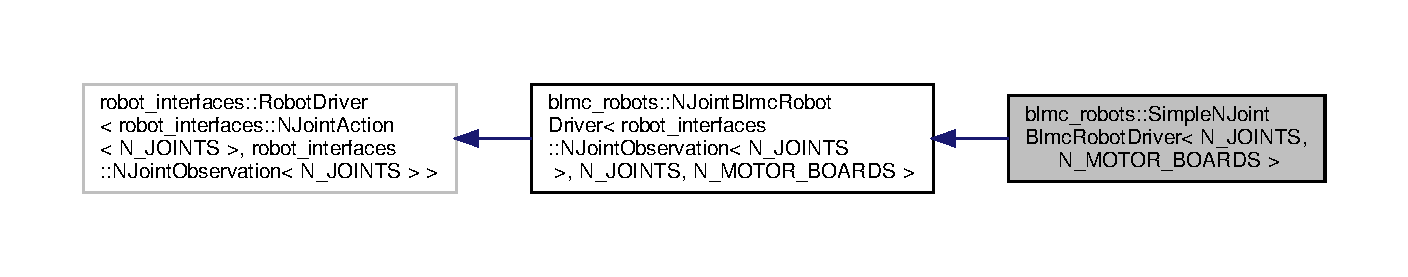
\includegraphics[width=350pt]{classblmc__robots_1_1SimpleNJointBlmcRobotDriver__inherit__graph}
\end{center}
\end{figure}


Collaboration diagram for blmc\+\_\+robots\+:\+:Simple\+N\+Joint\+Blmc\+Robot\+Driver$<$ N\+\_\+\+J\+O\+I\+N\+TS, N\+\_\+\+M\+O\+T\+O\+R\+\_\+\+B\+O\+A\+R\+DS $>$\+:
\nopagebreak
\begin{figure}[H]
\begin{center}
\leavevmode
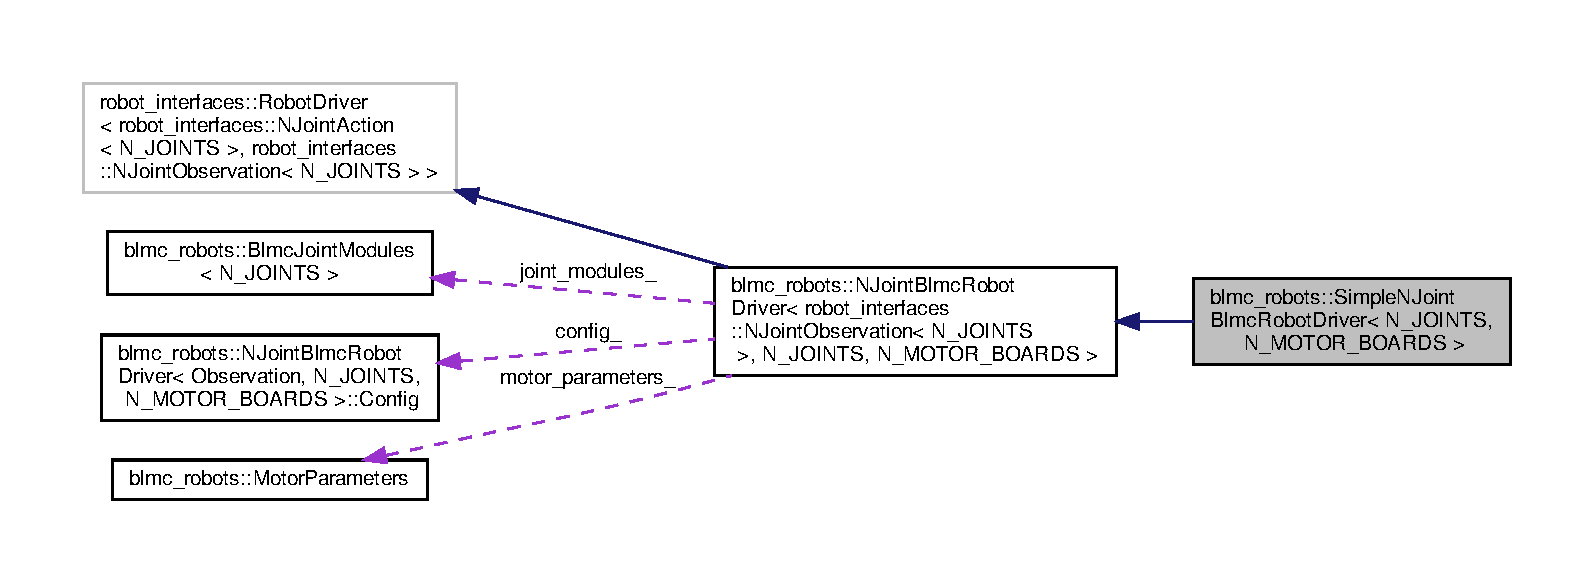
\includegraphics[width=350pt]{classblmc__robots_1_1SimpleNJointBlmcRobotDriver__coll__graph}
\end{center}
\end{figure}
\subsection*{Public Types}
\begin{DoxyCompactItemize}
\item 
\mbox{\Hypertarget{classblmc__robots_1_1SimpleNJointBlmcRobotDriver_aa916b4903890975830f4938d08909038}\label{classblmc__robots_1_1SimpleNJointBlmcRobotDriver_aa916b4903890975830f4938d08909038}} 
typedef robot\+\_\+interfaces\+::\+N\+Joint\+Observation$<$ N\+\_\+\+J\+O\+I\+N\+TS $>$ {\bfseries Observation}
\end{DoxyCompactItemize}
\subsection*{Public Member Functions}
\begin{DoxyCompactItemize}
\item 
\mbox{\Hypertarget{classblmc__robots_1_1SimpleNJointBlmcRobotDriver_a47bf814e68498f5344bd81c3d52906bc}\label{classblmc__robots_1_1SimpleNJointBlmcRobotDriver_a47bf814e68498f5344bd81c3d52906bc}} 
Observation {\bfseries get\+\_\+latest\+\_\+observation} () override
\end{DoxyCompactItemize}
\subsection*{Additional Inherited Members}


\subsection{Detailed Description}
\subsubsection*{template$<$size\+\_\+t N\+\_\+\+J\+O\+I\+N\+TS, size\+\_\+t N\+\_\+\+M\+O\+T\+O\+R\+\_\+\+B\+O\+A\+R\+DS = (\+N\+\_\+\+J\+O\+I\+N\+T\+S + 1) / 2$>$\newline
class blmc\+\_\+robots\+::\+Simple\+N\+Joint\+Blmc\+Robot\+Driver$<$ N\+\_\+\+J\+O\+I\+N\+T\+S, N\+\_\+\+M\+O\+T\+O\+R\+\_\+\+B\+O\+A\+R\+D\+S $>$}

Simple n-\/joint robot driver that uses N\+Joint\+Observation. 


\begin{DoxyTemplParams}{Template Parameters}
{\em N\+\_\+\+J\+O\+I\+N\+TS} & Number of joints \\
\hline
{\em N\+\_\+\+M\+O\+T\+O\+R\+\_\+\+B\+O\+A\+R\+DS} & Number of motor boards. \\
\hline
\end{DoxyTemplParams}


The documentation for this class was generated from the following files\+:\begin{DoxyCompactItemize}
\item 
include/blmc\+\_\+robots/\hyperlink{n__joint__blmc__robot__driver_8hpp}{n\+\_\+joint\+\_\+blmc\+\_\+robot\+\_\+driver.\+hpp}\item 
include/blmc\+\_\+robots/\hyperlink{n__joint__blmc__robot__driver_8hxx}{n\+\_\+joint\+\_\+blmc\+\_\+robot\+\_\+driver.\+hxx}\end{DoxyCompactItemize}

\hypertarget{classblmc__robots_1_1SingleLeg}{}\section{blmc\+\_\+robots\+:\+:Single\+Leg Class Reference}
\label{classblmc__robots_1_1SingleLeg}\index{blmc\+\_\+robots\+::\+Single\+Leg@{blmc\+\_\+robots\+::\+Single\+Leg}}
\subsection*{Public Types}
\begin{DoxyCompactItemize}
\item 
\mbox{\Hypertarget{classblmc__robots_1_1SingleLeg_a37fdbf57313957a5773cb13f2ad7190c}\label{classblmc__robots_1_1SingleLeg_a37fdbf57313957a5773cb13f2ad7190c}} 
typedef Eigen\+::\+Matrix$<$ double, 2, 1 $>$ {\bfseries Vector2d}
\item 
\mbox{\Hypertarget{classblmc__robots_1_1SingleLeg_a926cd2dfc01483687d44259874450757}\label{classblmc__robots_1_1SingleLeg_a926cd2dfc01483687d44259874450757}} 
typedef Eigen\+::\+Matrix$<$ double, 2, 1 $>$ {\bfseries Vector\+Slider}
\end{DoxyCompactItemize}
\subsection*{Public Member Functions}
\begin{DoxyCompactItemize}
\item 
\hyperlink{classblmc__robots_1_1SingleLeg_a1b1ef6964010aa2042b042ff3d5d864f}{Single\+Leg} ()
\begin{DoxyCompactList}\small\item\em \hyperlink{classblmc__robots_1_1SingleLeg}{Single\+Leg} is the constructor of the class. \end{DoxyCompactList}\item 
\mbox{\Hypertarget{classblmc__robots_1_1SingleLeg_a28891a4273cdcabc67bfd04dae75e8db}\label{classblmc__robots_1_1SingleLeg_a28891a4273cdcabc67bfd04dae75e8db}} 
void \hyperlink{classblmc__robots_1_1SingleLeg_a28891a4273cdcabc67bfd04dae75e8db}{initialize} ()
\begin{DoxyCompactList}\small\item\em initialize the robot by setting aligning the motors and calibrate the sensors to 0 \end{DoxyCompactList}\item 
\mbox{\Hypertarget{classblmc__robots_1_1SingleLeg_ac68163f459be877af9fb78f348729f9b}\label{classblmc__robots_1_1SingleLeg_ac68163f459be877af9fb78f348729f9b}} 
void \hyperlink{classblmc__robots_1_1SingleLeg_ac68163f459be877af9fb78f348729f9b}{send\+\_\+target\+\_\+motor\+\_\+current} (const Eigen\+::\+Ref$<$ Vector2d $>$ target\+\_\+motor\+\_\+current)
\begin{DoxyCompactList}\small\item\em send\+\_\+target\+\_\+torques sends the target currents to the motors \end{DoxyCompactList}\item 
\mbox{\Hypertarget{classblmc__robots_1_1SingleLeg_a0525a29e9b76527936525ca0e47cafe0}\label{classblmc__robots_1_1SingleLeg_a0525a29e9b76527936525ca0e47cafe0}} 
void \hyperlink{classblmc__robots_1_1SingleLeg_a0525a29e9b76527936525ca0e47cafe0}{send\+\_\+target\+\_\+joint\+\_\+torque} (const Eigen\+::\+Ref$<$ Vector2d $>$ target\+\_\+joint\+\_\+torque)
\begin{DoxyCompactList}\small\item\em send\+\_\+target\+\_\+torques sends the target currents to the motors \end{DoxyCompactList}\item 
void \hyperlink{classblmc__robots_1_1SingleLeg_a093a696ad34f00e92adcc4eb282a37d9}{acquire\+\_\+sensors} ()
\begin{DoxyCompactList}\small\item\em acquire\+\_\+sensors acquire all available sensors, W\+A\+R\+N\+I\+NG !!!! this method has to be called prior to any gettter to have up to date data. \end{DoxyCompactList}\item 
\mbox{\Hypertarget{classblmc__robots_1_1SingleLeg_a2d95b70a9aca9f7faf503fd5c62f067f}\label{classblmc__robots_1_1SingleLeg_a2d95b70a9aca9f7faf503fd5c62f067f}} 
void \hyperlink{classblmc__robots_1_1SingleLeg_a2d95b70a9aca9f7faf503fd5c62f067f}{zero\+\_\+joint\+\_\+positions} ()
\begin{DoxyCompactList}\small\item\em zero\+\_\+joint\+\_\+positions Use the current motor position to set the zero position for the joint angles. \end{DoxyCompactList}\item 
\mbox{\Hypertarget{classblmc__robots_1_1SingleLeg_a39c69c6578b42df3d556e8a23c3e1861}\label{classblmc__robots_1_1SingleLeg_a39c69c6578b42df3d556e8a23c3e1861}} 
void \hyperlink{classblmc__robots_1_1SingleLeg_a39c69c6578b42df3d556e8a23c3e1861}{disable\+\_\+can\+\_\+recv\+\_\+timeout} ()
\begin{DoxyCompactList}\small\item\em disable\+\_\+can\+\_\+recv\+\_\+timeout Disable the disable\+\_\+can\+\_\+recv\+\_\+timeout for all can boards. \end{DoxyCompactList}\item 
const Eigen\+::\+Ref$<$ Vector2d $>$ \hyperlink{classblmc__robots_1_1SingleLeg_a52324fdf9779bb82141e2056b222b30f}{get\+\_\+motor\+\_\+positions} ()
\begin{DoxyCompactList}\small\item\em get\+\_\+motor\+\_\+positions \end{DoxyCompactList}\item 
const Eigen\+::\+Ref$<$ Vector2d $>$ \hyperlink{classblmc__robots_1_1SingleLeg_afd9b40fdddedd93e2a92114862846a5e}{get\+\_\+motor\+\_\+velocities} ()
\begin{DoxyCompactList}\small\item\em get\+\_\+motor\+\_\+velocities \end{DoxyCompactList}\item 
const Eigen\+::\+Ref$<$ Vector2d $>$ \hyperlink{classblmc__robots_1_1SingleLeg_a6f9fea8b21a7fb58a95882ec3fe78a8d}{get\+\_\+motor\+\_\+currents} ()
\begin{DoxyCompactList}\small\item\em get\+\_\+motor\+\_\+currents \end{DoxyCompactList}\item 
const Eigen\+::\+Ref$<$ Vector2d $>$ \hyperlink{classblmc__robots_1_1SingleLeg_aeae6fa29a8a5019d11a7aab9dd443e98}{get\+\_\+motor\+\_\+target\+\_\+currents} ()
\begin{DoxyCompactList}\small\item\em get\+\_\+motor\+\_\+target\+\_\+currents \end{DoxyCompactList}\item 
const Eigen\+::\+Ref$<$ Vector2d $>$ \hyperlink{classblmc__robots_1_1SingleLeg_a11751bde3377207e56ded343e00a99f1}{get\+\_\+motor\+\_\+torques} ()
\begin{DoxyCompactList}\small\item\em get\+\_\+motor\+\_\+torques \end{DoxyCompactList}\item 
const Eigen\+::\+Ref$<$ Vector2d $>$ \hyperlink{classblmc__robots_1_1SingleLeg_a9f3277dbc3bc672e09dbdb51b7818d42}{get\+\_\+target\+\_\+motor\+\_\+torques} ()
\begin{DoxyCompactList}\small\item\em get\+\_\+target\+\_\+motor\+\_\+torques \end{DoxyCompactList}\item 
const Eigen\+::\+Ref$<$ Vector2d $>$ \hyperlink{classblmc__robots_1_1SingleLeg_a2be0f81bd58416d43614e2c6069ca471}{get\+\_\+motor\+\_\+inertias} ()
\begin{DoxyCompactList}\small\item\em get\+\_\+motor\+\_\+inertias \end{DoxyCompactList}\item 
const Eigen\+::\+Ref$<$ Vector2d $>$ \hyperlink{classblmc__robots_1_1SingleLeg_aec4353d090ed7bd503d43b3e17671ded}{get\+\_\+motor\+\_\+encoder\+\_\+indexes} ()
\begin{DoxyCompactList}\small\item\em get\+\_\+motor\+\_\+encoder\+\_\+indexes \end{DoxyCompactList}\item 
const Eigen\+::\+Ref$<$ Vector2d $>$ \hyperlink{classblmc__robots_1_1SingleLeg_a402a4e609e17fb304a113cb5c434b7e3}{get\+\_\+motor\+\_\+torque\+\_\+constants} ()
\begin{DoxyCompactList}\small\item\em get\+\_\+motor\+\_\+torque\+\_\+constants \end{DoxyCompactList}\item 
const Eigen\+::\+Ref$<$ Vector2d $>$ \hyperlink{classblmc__robots_1_1SingleLeg_ad69364827ba1f041bb45aec9ff678a74}{get\+\_\+joint\+\_\+positions} ()
\begin{DoxyCompactList}\small\item\em get\+\_\+joint\+\_\+positions \end{DoxyCompactList}\item 
const Eigen\+::\+Ref$<$ Vector2d $>$ \hyperlink{classblmc__robots_1_1SingleLeg_aad4d838300a95db9e5e78aa465601591}{get\+\_\+joint\+\_\+velocities} ()
\begin{DoxyCompactList}\small\item\em get\+\_\+joint\+\_\+velocities \end{DoxyCompactList}\item 
const Eigen\+::\+Ref$<$ Vector2d $>$ \hyperlink{classblmc__robots_1_1SingleLeg_adba890cb19a75df119a94d2f3b063ec2}{get\+\_\+joint\+\_\+torques} ()
\begin{DoxyCompactList}\small\item\em get\+\_\+joint\+\_\+torques \end{DoxyCompactList}\item 
const Eigen\+::\+Ref$<$ Vector2d $>$ \hyperlink{classblmc__robots_1_1SingleLeg_ab28eb09362cee1b0eaa1a066d5f4d760}{get\+\_\+joint\+\_\+target\+\_\+torques} ()
\begin{DoxyCompactList}\small\item\em get\+\_\+joint\+\_\+torques \end{DoxyCompactList}\item 
const Eigen\+::\+Ref$<$ Vector2d $>$ \hyperlink{classblmc__robots_1_1SingleLeg_ac697752c8bd67dc1f58360dbe46e57a6}{get\+\_\+joint\+\_\+gear\+\_\+ratios} ()
\begin{DoxyCompactList}\small\item\em get\+\_\+joint\+\_\+gear\+\_\+ratios \end{DoxyCompactList}\item 
const Eigen\+::\+Ref$<$ Vector2d $>$ \hyperlink{classblmc__robots_1_1SingleLeg_a3048925f67d4585e45200e6de05b73ac}{get\+\_\+joint\+\_\+encoder\+\_\+index} ()
\begin{DoxyCompactList}\small\item\em get\+\_\+joint\+\_\+encoder\+\_\+index \end{DoxyCompactList}\item 
const Eigen\+::\+Ref$<$ Vector2d $>$ \hyperlink{classblmc__robots_1_1SingleLeg_a010c3169b55ae8bab809efaa986987a3}{get\+\_\+zero\+\_\+positions} ()
\begin{DoxyCompactList}\small\item\em get\+\_\+zero\+\_\+positions \end{DoxyCompactList}\item 
const Eigen\+::\+Ref$<$ Vector2d $>$ \hyperlink{classblmc__robots_1_1SingleLeg_aa0b97287dcf0195fe918e1b4c0e7b470}{get\+\_\+slider\+\_\+positions} ()
\begin{DoxyCompactList}\small\item\em get\+\_\+slider\+\_\+positions \end{DoxyCompactList}\item 
const Eigen\+::\+Ref$<$ Vector2d $>$ \hyperlink{classblmc__robots_1_1SingleLeg_a662082708a0f24a120306e07490a0b70}{get\+\_\+max\+\_\+current} ()
\begin{DoxyCompactList}\small\item\em get\+\_\+max\+\_\+current \end{DoxyCompactList}\item 
const Eigen\+::\+Ref$<$ Vector2d $>$ \hyperlink{classblmc__robots_1_1SingleLeg_ace93cc10397888f07ecf5e14583535f9}{get\+\_\+max\+\_\+joint\+\_\+torque} ()
\begin{DoxyCompactList}\small\item\em get\+\_\+max\+\_\+torque \end{DoxyCompactList}\item 
void \hyperlink{classblmc__robots_1_1SingleLeg_a54007e95c258ec05b63169f202d3a3a0}{set\+\_\+max\+\_\+current} (const Eigen\+::\+Ref$<$ Vector2d $>$ max\+\_\+current)
\begin{DoxyCompactList}\small\item\em set\+\_\+max\+\_\+current sets the maximum current that the motor can to apply. \end{DoxyCompactList}\end{DoxyCompactItemize}
\subsection*{Private Attributes}
\begin{DoxyCompactItemize}
\item 
Vector2d \hyperlink{classblmc__robots_1_1SingleLeg_aca1dec9ed5af5052f23942731ac99386}{motor\+\_\+positions\+\_\+}
\begin{DoxyCompactList}\small\item\em Motor data. \end{DoxyCompactList}\item 
\mbox{\Hypertarget{classblmc__robots_1_1SingleLeg_ad74f4bc6470b2595f76c1eed9f241a1c}\label{classblmc__robots_1_1SingleLeg_ad74f4bc6470b2595f76c1eed9f241a1c}} 
Vector2d \hyperlink{classblmc__robots_1_1SingleLeg_ad74f4bc6470b2595f76c1eed9f241a1c}{motor\+\_\+velocities\+\_\+}
\begin{DoxyCompactList}\small\item\em motor\+\_\+velocities\+\_\+ \end{DoxyCompactList}\item 
\mbox{\Hypertarget{classblmc__robots_1_1SingleLeg_ab413e5ad446472e722874e579b2ea8a8}\label{classblmc__robots_1_1SingleLeg_ab413e5ad446472e722874e579b2ea8a8}} 
Vector2d \hyperlink{classblmc__robots_1_1SingleLeg_ab413e5ad446472e722874e579b2ea8a8}{motor\+\_\+currents\+\_\+}
\begin{DoxyCompactList}\small\item\em motor\+\_\+currents\+\_\+ \end{DoxyCompactList}\item 
\mbox{\Hypertarget{classblmc__robots_1_1SingleLeg_a08fb7a64361ca008694995d7dda73229}\label{classblmc__robots_1_1SingleLeg_a08fb7a64361ca008694995d7dda73229}} 
Vector2d \hyperlink{classblmc__robots_1_1SingleLeg_a08fb7a64361ca008694995d7dda73229}{motor\+\_\+torques\+\_\+}
\begin{DoxyCompactList}\small\item\em motor\+\_\+torques\+\_\+ \end{DoxyCompactList}\item 
\mbox{\Hypertarget{classblmc__robots_1_1SingleLeg_a53d12d5e709c863be176643697785729}\label{classblmc__robots_1_1SingleLeg_a53d12d5e709c863be176643697785729}} 
Vector2d \hyperlink{classblmc__robots_1_1SingleLeg_a53d12d5e709c863be176643697785729}{motor\+\_\+inertias\+\_\+}
\begin{DoxyCompactList}\small\item\em motor\+\_\+inertias\+\_\+ \end{DoxyCompactList}\item 
\mbox{\Hypertarget{classblmc__robots_1_1SingleLeg_a8ac67df4a61c02ca927bbcab5c4bab0b}\label{classblmc__robots_1_1SingleLeg_a8ac67df4a61c02ca927bbcab5c4bab0b}} 
Vector2d \hyperlink{classblmc__robots_1_1SingleLeg_a8ac67df4a61c02ca927bbcab5c4bab0b}{motor\+\_\+encoder\+\_\+indexes\+\_\+}
\begin{DoxyCompactList}\small\item\em motor\+\_\+encoder\+\_\+indexes\+\_\+ \end{DoxyCompactList}\item 
\mbox{\Hypertarget{classblmc__robots_1_1SingleLeg_a1727423baf1d924c5c38b5da82760daa}\label{classblmc__robots_1_1SingleLeg_a1727423baf1d924c5c38b5da82760daa}} 
Vector2d \hyperlink{classblmc__robots_1_1SingleLeg_a1727423baf1d924c5c38b5da82760daa}{motor\+\_\+target\+\_\+currents\+\_\+}
\begin{DoxyCompactList}\small\item\em motor\+\_\+target\+\_\+currents\+\_\+ \end{DoxyCompactList}\item 
\mbox{\Hypertarget{classblmc__robots_1_1SingleLeg_a877ea486d60de86dda6f2f584483cd63}\label{classblmc__robots_1_1SingleLeg_a877ea486d60de86dda6f2f584483cd63}} 
Vector2d \hyperlink{classblmc__robots_1_1SingleLeg_a877ea486d60de86dda6f2f584483cd63}{motor\+\_\+target\+\_\+torques\+\_\+}
\begin{DoxyCompactList}\small\item\em motor\+\_\+target\+\_\+torques\+\_\+ \end{DoxyCompactList}\item 
\mbox{\Hypertarget{classblmc__robots_1_1SingleLeg_acc9db4fea29151b45841b63a75d6cb18}\label{classblmc__robots_1_1SingleLeg_acc9db4fea29151b45841b63a75d6cb18}} 
Vector2d \hyperlink{classblmc__robots_1_1SingleLeg_acc9db4fea29151b45841b63a75d6cb18}{motor\+\_\+torque\+\_\+constants\+\_\+}
\begin{DoxyCompactList}\small\item\em motor\+\_\+torque\+\_\+constants\+\_\+ are the motor torque constants \end{DoxyCompactList}\item 
\mbox{\Hypertarget{classblmc__robots_1_1SingleLeg_a5408963ab970855f3ab0c5fc0fb51803}\label{classblmc__robots_1_1SingleLeg_a5408963ab970855f3ab0c5fc0fb51803}} 
Vector2d \hyperlink{classblmc__robots_1_1SingleLeg_a5408963ab970855f3ab0c5fc0fb51803}{target\+\_\+motor\+\_\+current\+\_\+tmp\+\_\+}
\begin{DoxyCompactList}\small\item\em target\+\_\+motor\+\_\+current\+\_\+tmp\+\_\+ is used to convert the joint torque to motor current \end{DoxyCompactList}\item 
Vector2d \hyperlink{classblmc__robots_1_1SingleLeg_ad74d44ab47c78a46c2ba6a7aa9e71750}{joint\+\_\+positions\+\_\+}
\begin{DoxyCompactList}\small\item\em Joint data. \end{DoxyCompactList}\item 
\mbox{\Hypertarget{classblmc__robots_1_1SingleLeg_ac383a1f260a35e47584ae7dd79be801c}\label{classblmc__robots_1_1SingleLeg_ac383a1f260a35e47584ae7dd79be801c}} 
Vector2d \hyperlink{classblmc__robots_1_1SingleLeg_ac383a1f260a35e47584ae7dd79be801c}{joint\+\_\+velocities\+\_\+}
\begin{DoxyCompactList}\small\item\em joint\+\_\+velocities\+\_\+ \end{DoxyCompactList}\item 
\mbox{\Hypertarget{classblmc__robots_1_1SingleLeg_a1662005c929cff8e429ead0d5bbdee87}\label{classblmc__robots_1_1SingleLeg_a1662005c929cff8e429ead0d5bbdee87}} 
Vector2d \hyperlink{classblmc__robots_1_1SingleLeg_a1662005c929cff8e429ead0d5bbdee87}{joint\+\_\+torques\+\_\+}
\begin{DoxyCompactList}\small\item\em joint\+\_\+torques\+\_\+ \end{DoxyCompactList}\item 
\mbox{\Hypertarget{classblmc__robots_1_1SingleLeg_a9c62fe22181054c020d0e10d1a68926c}\label{classblmc__robots_1_1SingleLeg_a9c62fe22181054c020d0e10d1a68926c}} 
Vector2d \hyperlink{classblmc__robots_1_1SingleLeg_a9c62fe22181054c020d0e10d1a68926c}{joint\+\_\+target\+\_\+torques\+\_\+}
\begin{DoxyCompactList}\small\item\em joint\+\_\+target\+\_\+torques\+\_\+ \end{DoxyCompactList}\item 
\mbox{\Hypertarget{classblmc__robots_1_1SingleLeg_a99bc5106cd51eb315fc4b7a6d19da9ed}\label{classblmc__robots_1_1SingleLeg_a99bc5106cd51eb315fc4b7a6d19da9ed}} 
Vector2d \hyperlink{classblmc__robots_1_1SingleLeg_a99bc5106cd51eb315fc4b7a6d19da9ed}{joint\+\_\+gear\+\_\+ratios\+\_\+}
\begin{DoxyCompactList}\small\item\em joint\+\_\+gear\+\_\+ratios are the joint gear ratios \end{DoxyCompactList}\item 
\mbox{\Hypertarget{classblmc__robots_1_1SingleLeg_a7b56a40d83103f77cd01915c6ee29367}\label{classblmc__robots_1_1SingleLeg_a7b56a40d83103f77cd01915c6ee29367}} 
Vector2d \hyperlink{classblmc__robots_1_1SingleLeg_a7b56a40d83103f77cd01915c6ee29367}{joint\+\_\+encoder\+\_\+index\+\_\+}
\begin{DoxyCompactList}\small\item\em joint\+\_\+encoder\+\_\+index\+\_\+ The last observed encoder\+\_\+index at the joints. \end{DoxyCompactList}\item 
\mbox{\Hypertarget{classblmc__robots_1_1SingleLeg_a757c6d5527c7914bdb30b8ee96a8df8d}\label{classblmc__robots_1_1SingleLeg_a757c6d5527c7914bdb30b8ee96a8df8d}} 
Vector2d \hyperlink{classblmc__robots_1_1SingleLeg_a757c6d5527c7914bdb30b8ee96a8df8d}{joint\+\_\+zero\+\_\+positions\+\_\+}
\begin{DoxyCompactList}\small\item\em joint\+\_\+zero\+\_\+positions\+\_\+ is the configuration considered as zero position \end{DoxyCompactList}\item 
\mbox{\Hypertarget{classblmc__robots_1_1SingleLeg_afb76b1c90cce0d805aa4baaa9b4de797}\label{classblmc__robots_1_1SingleLeg_afb76b1c90cce0d805aa4baaa9b4de797}} 
Vector2d \hyperlink{classblmc__robots_1_1SingleLeg_afb76b1c90cce0d805aa4baaa9b4de797}{joint\+\_\+max\+\_\+torque\+\_\+}
\begin{DoxyCompactList}\small\item\em joint\+\_\+max\+\_\+torque\+\_\+ \end{DoxyCompactList}\item 
Vector2d \hyperlink{classblmc__robots_1_1SingleLeg_af841dc84f18c70c85bb0e19dd88da85f}{slider\+\_\+positions\+\_\+}
\begin{DoxyCompactList}\small\item\em Additional data. \end{DoxyCompactList}\item 
\mbox{\Hypertarget{classblmc__robots_1_1SingleLeg_a4f8e64b30e001d4b1c74595841c26735}\label{classblmc__robots_1_1SingleLeg_a4f8e64b30e001d4b1c74595841c26735}} 
Vector2d \hyperlink{classblmc__robots_1_1SingleLeg_a4f8e64b30e001d4b1c74595841c26735}{motor\+\_\+max\+\_\+current\+\_\+}
\begin{DoxyCompactList}\small\item\em max\+\_\+current\+\_\+ is the current limit to be send to the motors, this a safe guard for development \end{DoxyCompactList}\item 
std\+::array$<$ \hyperlink{common__header_8hpp_a793c8789a7598e8aaf766939da7262af}{Can\+Bus\+\_\+ptr}, 1 $>$ \hyperlink{classblmc__robots_1_1SingleLeg_a021418412c79cfa868bfffec24155ef8}{can\+\_\+buses\+\_\+}
\begin{DoxyCompactList}\small\item\em Drivers communication objects. \end{DoxyCompactList}\item 
\mbox{\Hypertarget{classblmc__robots_1_1SingleLeg_a133902cdf8468f2cf8849fdc6daed312}\label{classblmc__robots_1_1SingleLeg_a133902cdf8468f2cf8849fdc6daed312}} 
std\+::array$<$ \hyperlink{common__header_8hpp_aab1c6ddb1273247a1b45d5e8b417c216}{Can\+Bus\+Motor\+Board\+\_\+ptr}, 1 $>$ \hyperlink{classblmc__robots_1_1SingleLeg_a133902cdf8468f2cf8849fdc6daed312}{can\+\_\+motor\+\_\+boards\+\_\+}
\begin{DoxyCompactList}\small\item\em can\+\_\+motor\+\_\+boards\+\_\+ are the 4 can motor board. \end{DoxyCompactList}\item 
\mbox{\Hypertarget{classblmc__robots_1_1SingleLeg_ac2964b955b883496833cd5d00ab2b1c7}\label{classblmc__robots_1_1SingleLeg_ac2964b955b883496833cd5d00ab2b1c7}} 
std\+::array$<$ \hyperlink{common__header_8hpp_a9850cf917156e20846aef3f8195aea0f}{Safe\+Motor\+\_\+ptr}, 2 $>$ \hyperlink{classblmc__robots_1_1SingleLeg_ac2964b955b883496833cd5d00ab2b1c7}{motors\+\_\+}
\begin{DoxyCompactList}\small\item\em motors\+\_\+ are the objects alowing us to send motor commands and receive data \end{DoxyCompactList}\item 
\mbox{\Hypertarget{classblmc__robots_1_1SingleLeg_a009823b7c3e817eabb6e572406460d2f}\label{classblmc__robots_1_1SingleLeg_a009823b7c3e817eabb6e572406460d2f}} 
std\+::array$<$ \hyperlink{common__header_8hpp_a4cb9a95e8b2c0bf237ce29f5252c7b73}{Slider\+\_\+ptr}, 2 $>$ \hyperlink{classblmc__robots_1_1SingleLeg_a009823b7c3e817eabb6e572406460d2f}{sliders\+\_\+}
\begin{DoxyCompactList}\small\item\em sliders\+\_\+ these are analogue input from linear potentiometers. \end{DoxyCompactList}\end{DoxyCompactItemize}


\subsection{Constructor \& Destructor Documentation}
\mbox{\Hypertarget{classblmc__robots_1_1SingleLeg_a1b1ef6964010aa2042b042ff3d5d864f}\label{classblmc__robots_1_1SingleLeg_a1b1ef6964010aa2042b042ff3d5d864f}} 
\index{blmc\+\_\+robots\+::\+Single\+Leg@{blmc\+\_\+robots\+::\+Single\+Leg}!Single\+Leg@{Single\+Leg}}
\index{Single\+Leg@{Single\+Leg}!blmc\+\_\+robots\+::\+Single\+Leg@{blmc\+\_\+robots\+::\+Single\+Leg}}
\subsubsection{\texorpdfstring{Single\+Leg()}{SingleLeg()}}
{\footnotesize\ttfamily blmc\+\_\+robots\+::\+Single\+Leg\+::\+Single\+Leg (\begin{DoxyParamCaption}{ }\end{DoxyParamCaption})}



\hyperlink{classblmc__robots_1_1SingleLeg}{Single\+Leg} is the constructor of the class. 

Motor data

Joint data

Additional data

Setup some known data

\subsection{Member Function Documentation}
\mbox{\Hypertarget{classblmc__robots_1_1SingleLeg_a093a696ad34f00e92adcc4eb282a37d9}\label{classblmc__robots_1_1SingleLeg_a093a696ad34f00e92adcc4eb282a37d9}} 
\index{blmc\+\_\+robots\+::\+Single\+Leg@{blmc\+\_\+robots\+::\+Single\+Leg}!acquire\+\_\+sensors@{acquire\+\_\+sensors}}
\index{acquire\+\_\+sensors@{acquire\+\_\+sensors}!blmc\+\_\+robots\+::\+Single\+Leg@{blmc\+\_\+robots\+::\+Single\+Leg}}
\subsubsection{\texorpdfstring{acquire\+\_\+sensors()}{acquire\_sensors()}}
{\footnotesize\ttfamily void blmc\+\_\+robots\+::\+Single\+Leg\+::acquire\+\_\+sensors (\begin{DoxyParamCaption}{ }\end{DoxyParamCaption})}



acquire\+\_\+sensors acquire all available sensors, W\+A\+R\+N\+I\+NG !!!! this method has to be called prior to any gettter to have up to date data. 

Motor data

Joint data

Additional data\mbox{\Hypertarget{classblmc__robots_1_1SingleLeg_a3048925f67d4585e45200e6de05b73ac}\label{classblmc__robots_1_1SingleLeg_a3048925f67d4585e45200e6de05b73ac}} 
\index{blmc\+\_\+robots\+::\+Single\+Leg@{blmc\+\_\+robots\+::\+Single\+Leg}!get\+\_\+joint\+\_\+encoder\+\_\+index@{get\+\_\+joint\+\_\+encoder\+\_\+index}}
\index{get\+\_\+joint\+\_\+encoder\+\_\+index@{get\+\_\+joint\+\_\+encoder\+\_\+index}!blmc\+\_\+robots\+::\+Single\+Leg@{blmc\+\_\+robots\+::\+Single\+Leg}}
\subsubsection{\texorpdfstring{get\+\_\+joint\+\_\+encoder\+\_\+index()}{get\_joint\_encoder\_index()}}
{\footnotesize\ttfamily const Eigen\+::\+Ref$<$Vector2d$>$ blmc\+\_\+robots\+::\+Single\+Leg\+::get\+\_\+joint\+\_\+encoder\+\_\+index (\begin{DoxyParamCaption}{ }\end{DoxyParamCaption})\hspace{0.3cm}{\ttfamily [inline]}}



get\+\_\+joint\+\_\+encoder\+\_\+index 

\begin{DoxyReturn}{Returns}
The last observed encoder index in joint coordinates. 
\end{DoxyReturn}
\mbox{\Hypertarget{classblmc__robots_1_1SingleLeg_ac697752c8bd67dc1f58360dbe46e57a6}\label{classblmc__robots_1_1SingleLeg_ac697752c8bd67dc1f58360dbe46e57a6}} 
\index{blmc\+\_\+robots\+::\+Single\+Leg@{blmc\+\_\+robots\+::\+Single\+Leg}!get\+\_\+joint\+\_\+gear\+\_\+ratios@{get\+\_\+joint\+\_\+gear\+\_\+ratios}}
\index{get\+\_\+joint\+\_\+gear\+\_\+ratios@{get\+\_\+joint\+\_\+gear\+\_\+ratios}!blmc\+\_\+robots\+::\+Single\+Leg@{blmc\+\_\+robots\+::\+Single\+Leg}}
\subsubsection{\texorpdfstring{get\+\_\+joint\+\_\+gear\+\_\+ratios()}{get\_joint\_gear\_ratios()}}
{\footnotesize\ttfamily const Eigen\+::\+Ref$<$Vector2d$>$ blmc\+\_\+robots\+::\+Single\+Leg\+::get\+\_\+joint\+\_\+gear\+\_\+ratios (\begin{DoxyParamCaption}{ }\end{DoxyParamCaption})\hspace{0.3cm}{\ttfamily [inline]}}



get\+\_\+joint\+\_\+gear\+\_\+ratios 

\begin{DoxyReturn}{Returns}
the joint gear ratios 
\end{DoxyReturn}
\mbox{\Hypertarget{classblmc__robots_1_1SingleLeg_ad69364827ba1f041bb45aec9ff678a74}\label{classblmc__robots_1_1SingleLeg_ad69364827ba1f041bb45aec9ff678a74}} 
\index{blmc\+\_\+robots\+::\+Single\+Leg@{blmc\+\_\+robots\+::\+Single\+Leg}!get\+\_\+joint\+\_\+positions@{get\+\_\+joint\+\_\+positions}}
\index{get\+\_\+joint\+\_\+positions@{get\+\_\+joint\+\_\+positions}!blmc\+\_\+robots\+::\+Single\+Leg@{blmc\+\_\+robots\+::\+Single\+Leg}}
\subsubsection{\texorpdfstring{get\+\_\+joint\+\_\+positions()}{get\_joint\_positions()}}
{\footnotesize\ttfamily const Eigen\+::\+Ref$<$Vector2d$>$ blmc\+\_\+robots\+::\+Single\+Leg\+::get\+\_\+joint\+\_\+positions (\begin{DoxyParamCaption}{ }\end{DoxyParamCaption})\hspace{0.3cm}{\ttfamily [inline]}}



get\+\_\+joint\+\_\+positions 

\begin{DoxyReturn}{Returns}
the joint angle of each module 
\end{DoxyReturn}
\mbox{\Hypertarget{classblmc__robots_1_1SingleLeg_ab28eb09362cee1b0eaa1a066d5f4d760}\label{classblmc__robots_1_1SingleLeg_ab28eb09362cee1b0eaa1a066d5f4d760}} 
\index{blmc\+\_\+robots\+::\+Single\+Leg@{blmc\+\_\+robots\+::\+Single\+Leg}!get\+\_\+joint\+\_\+target\+\_\+torques@{get\+\_\+joint\+\_\+target\+\_\+torques}}
\index{get\+\_\+joint\+\_\+target\+\_\+torques@{get\+\_\+joint\+\_\+target\+\_\+torques}!blmc\+\_\+robots\+::\+Single\+Leg@{blmc\+\_\+robots\+::\+Single\+Leg}}
\subsubsection{\texorpdfstring{get\+\_\+joint\+\_\+target\+\_\+torques()}{get\_joint\_target\_torques()}}
{\footnotesize\ttfamily const Eigen\+::\+Ref$<$Vector2d$>$ blmc\+\_\+robots\+::\+Single\+Leg\+::get\+\_\+joint\+\_\+target\+\_\+torques (\begin{DoxyParamCaption}{ }\end{DoxyParamCaption})\hspace{0.3cm}{\ttfamily [inline]}}



get\+\_\+joint\+\_\+torques 

\begin{DoxyReturn}{Returns}
the target joint torques 
\end{DoxyReturn}
\mbox{\Hypertarget{classblmc__robots_1_1SingleLeg_adba890cb19a75df119a94d2f3b063ec2}\label{classblmc__robots_1_1SingleLeg_adba890cb19a75df119a94d2f3b063ec2}} 
\index{blmc\+\_\+robots\+::\+Single\+Leg@{blmc\+\_\+robots\+::\+Single\+Leg}!get\+\_\+joint\+\_\+torques@{get\+\_\+joint\+\_\+torques}}
\index{get\+\_\+joint\+\_\+torques@{get\+\_\+joint\+\_\+torques}!blmc\+\_\+robots\+::\+Single\+Leg@{blmc\+\_\+robots\+::\+Single\+Leg}}
\subsubsection{\texorpdfstring{get\+\_\+joint\+\_\+torques()}{get\_joint\_torques()}}
{\footnotesize\ttfamily const Eigen\+::\+Ref$<$Vector2d$>$ blmc\+\_\+robots\+::\+Single\+Leg\+::get\+\_\+joint\+\_\+torques (\begin{DoxyParamCaption}{ }\end{DoxyParamCaption})\hspace{0.3cm}{\ttfamily [inline]}}



get\+\_\+joint\+\_\+torques 

\begin{DoxyReturn}{Returns}
the joint torques 
\end{DoxyReturn}
\mbox{\Hypertarget{classblmc__robots_1_1SingleLeg_aad4d838300a95db9e5e78aa465601591}\label{classblmc__robots_1_1SingleLeg_aad4d838300a95db9e5e78aa465601591}} 
\index{blmc\+\_\+robots\+::\+Single\+Leg@{blmc\+\_\+robots\+::\+Single\+Leg}!get\+\_\+joint\+\_\+velocities@{get\+\_\+joint\+\_\+velocities}}
\index{get\+\_\+joint\+\_\+velocities@{get\+\_\+joint\+\_\+velocities}!blmc\+\_\+robots\+::\+Single\+Leg@{blmc\+\_\+robots\+::\+Single\+Leg}}
\subsubsection{\texorpdfstring{get\+\_\+joint\+\_\+velocities()}{get\_joint\_velocities()}}
{\footnotesize\ttfamily const Eigen\+::\+Ref$<$Vector2d$>$ blmc\+\_\+robots\+::\+Single\+Leg\+::get\+\_\+joint\+\_\+velocities (\begin{DoxyParamCaption}{ }\end{DoxyParamCaption})\hspace{0.3cm}{\ttfamily [inline]}}



get\+\_\+joint\+\_\+velocities 

\begin{DoxyReturn}{Returns}
the joint velocities 
\end{DoxyReturn}
\mbox{\Hypertarget{classblmc__robots_1_1SingleLeg_a662082708a0f24a120306e07490a0b70}\label{classblmc__robots_1_1SingleLeg_a662082708a0f24a120306e07490a0b70}} 
\index{blmc\+\_\+robots\+::\+Single\+Leg@{blmc\+\_\+robots\+::\+Single\+Leg}!get\+\_\+max\+\_\+current@{get\+\_\+max\+\_\+current}}
\index{get\+\_\+max\+\_\+current@{get\+\_\+max\+\_\+current}!blmc\+\_\+robots\+::\+Single\+Leg@{blmc\+\_\+robots\+::\+Single\+Leg}}
\subsubsection{\texorpdfstring{get\+\_\+max\+\_\+current()}{get\_max\_current()}}
{\footnotesize\ttfamily const Eigen\+::\+Ref$<$Vector2d$>$ blmc\+\_\+robots\+::\+Single\+Leg\+::get\+\_\+max\+\_\+current (\begin{DoxyParamCaption}{ }\end{DoxyParamCaption})\hspace{0.3cm}{\ttfamily [inline]}}



get\+\_\+max\+\_\+current 

\begin{DoxyReturn}{Returns}
the max current that has been hard-\/coded in the constructor of this class. T\+O\+DO\+: parametrize this via Y\+A\+ML or something else. 
\end{DoxyReturn}
\mbox{\Hypertarget{classblmc__robots_1_1SingleLeg_ace93cc10397888f07ecf5e14583535f9}\label{classblmc__robots_1_1SingleLeg_ace93cc10397888f07ecf5e14583535f9}} 
\index{blmc\+\_\+robots\+::\+Single\+Leg@{blmc\+\_\+robots\+::\+Single\+Leg}!get\+\_\+max\+\_\+joint\+\_\+torque@{get\+\_\+max\+\_\+joint\+\_\+torque}}
\index{get\+\_\+max\+\_\+joint\+\_\+torque@{get\+\_\+max\+\_\+joint\+\_\+torque}!blmc\+\_\+robots\+::\+Single\+Leg@{blmc\+\_\+robots\+::\+Single\+Leg}}
\subsubsection{\texorpdfstring{get\+\_\+max\+\_\+joint\+\_\+torque()}{get\_max\_joint\_torque()}}
{\footnotesize\ttfamily const Eigen\+::\+Ref$<$Vector2d$>$ blmc\+\_\+robots\+::\+Single\+Leg\+::get\+\_\+max\+\_\+joint\+\_\+torque (\begin{DoxyParamCaption}{ }\end{DoxyParamCaption})\hspace{0.3cm}{\ttfamily [inline]}}



get\+\_\+max\+\_\+torque 

\begin{DoxyReturn}{Returns}
the max torque that has been hard-\/coded in the constructor of this class. T\+O\+DO\+: parametrize this via Y\+A\+ML or something else. 
\end{DoxyReturn}
\mbox{\Hypertarget{classblmc__robots_1_1SingleLeg_a6f9fea8b21a7fb58a95882ec3fe78a8d}\label{classblmc__robots_1_1SingleLeg_a6f9fea8b21a7fb58a95882ec3fe78a8d}} 
\index{blmc\+\_\+robots\+::\+Single\+Leg@{blmc\+\_\+robots\+::\+Single\+Leg}!get\+\_\+motor\+\_\+currents@{get\+\_\+motor\+\_\+currents}}
\index{get\+\_\+motor\+\_\+currents@{get\+\_\+motor\+\_\+currents}!blmc\+\_\+robots\+::\+Single\+Leg@{blmc\+\_\+robots\+::\+Single\+Leg}}
\subsubsection{\texorpdfstring{get\+\_\+motor\+\_\+currents()}{get\_motor\_currents()}}
{\footnotesize\ttfamily const Eigen\+::\+Ref$<$Vector2d$>$ blmc\+\_\+robots\+::\+Single\+Leg\+::get\+\_\+motor\+\_\+currents (\begin{DoxyParamCaption}{ }\end{DoxyParamCaption})\hspace{0.3cm}{\ttfamily [inline]}}



get\+\_\+motor\+\_\+currents 

\begin{DoxyReturn}{Returns}
the current motors currents in (Ampere\+: A). 
\end{DoxyReturn}
\mbox{\Hypertarget{classblmc__robots_1_1SingleLeg_aec4353d090ed7bd503d43b3e17671ded}\label{classblmc__robots_1_1SingleLeg_aec4353d090ed7bd503d43b3e17671ded}} 
\index{blmc\+\_\+robots\+::\+Single\+Leg@{blmc\+\_\+robots\+::\+Single\+Leg}!get\+\_\+motor\+\_\+encoder\+\_\+indexes@{get\+\_\+motor\+\_\+encoder\+\_\+indexes}}
\index{get\+\_\+motor\+\_\+encoder\+\_\+indexes@{get\+\_\+motor\+\_\+encoder\+\_\+indexes}!blmc\+\_\+robots\+::\+Single\+Leg@{blmc\+\_\+robots\+::\+Single\+Leg}}
\subsubsection{\texorpdfstring{get\+\_\+motor\+\_\+encoder\+\_\+indexes()}{get\_motor\_encoder\_indexes()}}
{\footnotesize\ttfamily const Eigen\+::\+Ref$<$Vector2d$>$ blmc\+\_\+robots\+::\+Single\+Leg\+::get\+\_\+motor\+\_\+encoder\+\_\+indexes (\begin{DoxyParamCaption}{ }\end{DoxyParamCaption})\hspace{0.3cm}{\ttfamily [inline]}}



get\+\_\+motor\+\_\+encoder\+\_\+indexes 

\begin{DoxyReturn}{Returns}
the position of the index of the encoders a the motor level 
\end{DoxyReturn}
\mbox{\Hypertarget{classblmc__robots_1_1SingleLeg_a2be0f81bd58416d43614e2c6069ca471}\label{classblmc__robots_1_1SingleLeg_a2be0f81bd58416d43614e2c6069ca471}} 
\index{blmc\+\_\+robots\+::\+Single\+Leg@{blmc\+\_\+robots\+::\+Single\+Leg}!get\+\_\+motor\+\_\+inertias@{get\+\_\+motor\+\_\+inertias}}
\index{get\+\_\+motor\+\_\+inertias@{get\+\_\+motor\+\_\+inertias}!blmc\+\_\+robots\+::\+Single\+Leg@{blmc\+\_\+robots\+::\+Single\+Leg}}
\subsubsection{\texorpdfstring{get\+\_\+motor\+\_\+inertias()}{get\_motor\_inertias()}}
{\footnotesize\ttfamily const Eigen\+::\+Ref$<$Vector2d$>$ blmc\+\_\+robots\+::\+Single\+Leg\+::get\+\_\+motor\+\_\+inertias (\begin{DoxyParamCaption}{ }\end{DoxyParamCaption})\hspace{0.3cm}{\ttfamily [inline]}}



get\+\_\+motor\+\_\+inertias 

\begin{DoxyReturn}{Returns}
the motor inertias 
\end{DoxyReturn}
\mbox{\Hypertarget{classblmc__robots_1_1SingleLeg_a52324fdf9779bb82141e2056b222b30f}\label{classblmc__robots_1_1SingleLeg_a52324fdf9779bb82141e2056b222b30f}} 
\index{blmc\+\_\+robots\+::\+Single\+Leg@{blmc\+\_\+robots\+::\+Single\+Leg}!get\+\_\+motor\+\_\+positions@{get\+\_\+motor\+\_\+positions}}
\index{get\+\_\+motor\+\_\+positions@{get\+\_\+motor\+\_\+positions}!blmc\+\_\+robots\+::\+Single\+Leg@{blmc\+\_\+robots\+::\+Single\+Leg}}
\subsubsection{\texorpdfstring{get\+\_\+motor\+\_\+positions()}{get\_motor\_positions()}}
{\footnotesize\ttfamily const Eigen\+::\+Ref$<$Vector2d$>$ blmc\+\_\+robots\+::\+Single\+Leg\+::get\+\_\+motor\+\_\+positions (\begin{DoxyParamCaption}{ }\end{DoxyParamCaption})\hspace{0.3cm}{\ttfamily [inline]}}



get\+\_\+motor\+\_\+positions 

\begin{DoxyReturn}{Returns}
the current motors positions (rad). 
\end{DoxyReturn}
\mbox{\Hypertarget{classblmc__robots_1_1SingleLeg_aeae6fa29a8a5019d11a7aab9dd443e98}\label{classblmc__robots_1_1SingleLeg_aeae6fa29a8a5019d11a7aab9dd443e98}} 
\index{blmc\+\_\+robots\+::\+Single\+Leg@{blmc\+\_\+robots\+::\+Single\+Leg}!get\+\_\+motor\+\_\+target\+\_\+currents@{get\+\_\+motor\+\_\+target\+\_\+currents}}
\index{get\+\_\+motor\+\_\+target\+\_\+currents@{get\+\_\+motor\+\_\+target\+\_\+currents}!blmc\+\_\+robots\+::\+Single\+Leg@{blmc\+\_\+robots\+::\+Single\+Leg}}
\subsubsection{\texorpdfstring{get\+\_\+motor\+\_\+target\+\_\+currents()}{get\_motor\_target\_currents()}}
{\footnotesize\ttfamily const Eigen\+::\+Ref$<$Vector2d$>$ blmc\+\_\+robots\+::\+Single\+Leg\+::get\+\_\+motor\+\_\+target\+\_\+currents (\begin{DoxyParamCaption}{ }\end{DoxyParamCaption})\hspace{0.3cm}{\ttfamily [inline]}}



get\+\_\+motor\+\_\+target\+\_\+currents 

\begin{DoxyReturn}{Returns}
the target current motors currents in (Ampere\+: A). 
\end{DoxyReturn}
\mbox{\Hypertarget{classblmc__robots_1_1SingleLeg_a402a4e609e17fb304a113cb5c434b7e3}\label{classblmc__robots_1_1SingleLeg_a402a4e609e17fb304a113cb5c434b7e3}} 
\index{blmc\+\_\+robots\+::\+Single\+Leg@{blmc\+\_\+robots\+::\+Single\+Leg}!get\+\_\+motor\+\_\+torque\+\_\+constants@{get\+\_\+motor\+\_\+torque\+\_\+constants}}
\index{get\+\_\+motor\+\_\+torque\+\_\+constants@{get\+\_\+motor\+\_\+torque\+\_\+constants}!blmc\+\_\+robots\+::\+Single\+Leg@{blmc\+\_\+robots\+::\+Single\+Leg}}
\subsubsection{\texorpdfstring{get\+\_\+motor\+\_\+torque\+\_\+constants()}{get\_motor\_torque\_constants()}}
{\footnotesize\ttfamily const Eigen\+::\+Ref$<$Vector2d$>$ blmc\+\_\+robots\+::\+Single\+Leg\+::get\+\_\+motor\+\_\+torque\+\_\+constants (\begin{DoxyParamCaption}{ }\end{DoxyParamCaption})\hspace{0.3cm}{\ttfamily [inline]}}



get\+\_\+motor\+\_\+torque\+\_\+constants 

\begin{DoxyReturn}{Returns}
the torque constants of each motor 
\end{DoxyReturn}
\mbox{\Hypertarget{classblmc__robots_1_1SingleLeg_a11751bde3377207e56ded343e00a99f1}\label{classblmc__robots_1_1SingleLeg_a11751bde3377207e56ded343e00a99f1}} 
\index{blmc\+\_\+robots\+::\+Single\+Leg@{blmc\+\_\+robots\+::\+Single\+Leg}!get\+\_\+motor\+\_\+torques@{get\+\_\+motor\+\_\+torques}}
\index{get\+\_\+motor\+\_\+torques@{get\+\_\+motor\+\_\+torques}!blmc\+\_\+robots\+::\+Single\+Leg@{blmc\+\_\+robots\+::\+Single\+Leg}}
\subsubsection{\texorpdfstring{get\+\_\+motor\+\_\+torques()}{get\_motor\_torques()}}
{\footnotesize\ttfamily const Eigen\+::\+Ref$<$Vector2d$>$ blmc\+\_\+robots\+::\+Single\+Leg\+::get\+\_\+motor\+\_\+torques (\begin{DoxyParamCaption}{ }\end{DoxyParamCaption})\hspace{0.3cm}{\ttfamily [inline]}}



get\+\_\+motor\+\_\+torques 

\begin{DoxyReturn}{Returns}
the motor torques in Nm 
\end{DoxyReturn}
\mbox{\Hypertarget{classblmc__robots_1_1SingleLeg_afd9b40fdddedd93e2a92114862846a5e}\label{classblmc__robots_1_1SingleLeg_afd9b40fdddedd93e2a92114862846a5e}} 
\index{blmc\+\_\+robots\+::\+Single\+Leg@{blmc\+\_\+robots\+::\+Single\+Leg}!get\+\_\+motor\+\_\+velocities@{get\+\_\+motor\+\_\+velocities}}
\index{get\+\_\+motor\+\_\+velocities@{get\+\_\+motor\+\_\+velocities}!blmc\+\_\+robots\+::\+Single\+Leg@{blmc\+\_\+robots\+::\+Single\+Leg}}
\subsubsection{\texorpdfstring{get\+\_\+motor\+\_\+velocities()}{get\_motor\_velocities()}}
{\footnotesize\ttfamily const Eigen\+::\+Ref$<$Vector2d$>$ blmc\+\_\+robots\+::\+Single\+Leg\+::get\+\_\+motor\+\_\+velocities (\begin{DoxyParamCaption}{ }\end{DoxyParamCaption})\hspace{0.3cm}{\ttfamily [inline]}}



get\+\_\+motor\+\_\+velocities 

\begin{DoxyReturn}{Returns}
the current motors velocities (rad/s). 
\end{DoxyReturn}
\mbox{\Hypertarget{classblmc__robots_1_1SingleLeg_aa0b97287dcf0195fe918e1b4c0e7b470}\label{classblmc__robots_1_1SingleLeg_aa0b97287dcf0195fe918e1b4c0e7b470}} 
\index{blmc\+\_\+robots\+::\+Single\+Leg@{blmc\+\_\+robots\+::\+Single\+Leg}!get\+\_\+slider\+\_\+positions@{get\+\_\+slider\+\_\+positions}}
\index{get\+\_\+slider\+\_\+positions@{get\+\_\+slider\+\_\+positions}!blmc\+\_\+robots\+::\+Single\+Leg@{blmc\+\_\+robots\+::\+Single\+Leg}}
\subsubsection{\texorpdfstring{get\+\_\+slider\+\_\+positions()}{get\_slider\_positions()}}
{\footnotesize\ttfamily const Eigen\+::\+Ref$<$Vector2d$>$ blmc\+\_\+robots\+::\+Single\+Leg\+::get\+\_\+slider\+\_\+positions (\begin{DoxyParamCaption}{ }\end{DoxyParamCaption})\hspace{0.3cm}{\ttfamily [inline]}}



get\+\_\+slider\+\_\+positions 

\begin{DoxyReturn}{Returns}
the current sliders positions. 
\end{DoxyReturn}
\mbox{\Hypertarget{classblmc__robots_1_1SingleLeg_a9f3277dbc3bc672e09dbdb51b7818d42}\label{classblmc__robots_1_1SingleLeg_a9f3277dbc3bc672e09dbdb51b7818d42}} 
\index{blmc\+\_\+robots\+::\+Single\+Leg@{blmc\+\_\+robots\+::\+Single\+Leg}!get\+\_\+target\+\_\+motor\+\_\+torques@{get\+\_\+target\+\_\+motor\+\_\+torques}}
\index{get\+\_\+target\+\_\+motor\+\_\+torques@{get\+\_\+target\+\_\+motor\+\_\+torques}!blmc\+\_\+robots\+::\+Single\+Leg@{blmc\+\_\+robots\+::\+Single\+Leg}}
\subsubsection{\texorpdfstring{get\+\_\+target\+\_\+motor\+\_\+torques()}{get\_target\_motor\_torques()}}
{\footnotesize\ttfamily const Eigen\+::\+Ref$<$Vector2d$>$ blmc\+\_\+robots\+::\+Single\+Leg\+::get\+\_\+target\+\_\+motor\+\_\+torques (\begin{DoxyParamCaption}{ }\end{DoxyParamCaption})\hspace{0.3cm}{\ttfamily [inline]}}



get\+\_\+target\+\_\+motor\+\_\+torques 

\begin{DoxyReturn}{Returns}
the target motor torques in Nm 
\end{DoxyReturn}
\mbox{\Hypertarget{classblmc__robots_1_1SingleLeg_a010c3169b55ae8bab809efaa986987a3}\label{classblmc__robots_1_1SingleLeg_a010c3169b55ae8bab809efaa986987a3}} 
\index{blmc\+\_\+robots\+::\+Single\+Leg@{blmc\+\_\+robots\+::\+Single\+Leg}!get\+\_\+zero\+\_\+positions@{get\+\_\+zero\+\_\+positions}}
\index{get\+\_\+zero\+\_\+positions@{get\+\_\+zero\+\_\+positions}!blmc\+\_\+robots\+::\+Single\+Leg@{blmc\+\_\+robots\+::\+Single\+Leg}}
\subsubsection{\texorpdfstring{get\+\_\+zero\+\_\+positions()}{get\_zero\_positions()}}
{\footnotesize\ttfamily const Eigen\+::\+Ref$<$Vector2d$>$ blmc\+\_\+robots\+::\+Single\+Leg\+::get\+\_\+zero\+\_\+positions (\begin{DoxyParamCaption}{ }\end{DoxyParamCaption})\hspace{0.3cm}{\ttfamily [inline]}}



get\+\_\+zero\+\_\+positions 

\begin{DoxyReturn}{Returns}
the position where the robot should be in \char`\"{}zero\char`\"{} configuration 
\end{DoxyReturn}
\mbox{\Hypertarget{classblmc__robots_1_1SingleLeg_a54007e95c258ec05b63169f202d3a3a0}\label{classblmc__robots_1_1SingleLeg_a54007e95c258ec05b63169f202d3a3a0}} 
\index{blmc\+\_\+robots\+::\+Single\+Leg@{blmc\+\_\+robots\+::\+Single\+Leg}!set\+\_\+max\+\_\+current@{set\+\_\+max\+\_\+current}}
\index{set\+\_\+max\+\_\+current@{set\+\_\+max\+\_\+current}!blmc\+\_\+robots\+::\+Single\+Leg@{blmc\+\_\+robots\+::\+Single\+Leg}}
\subsubsection{\texorpdfstring{set\+\_\+max\+\_\+current()}{set\_max\_current()}}
{\footnotesize\ttfamily void blmc\+\_\+robots\+::\+Single\+Leg\+::set\+\_\+max\+\_\+current (\begin{DoxyParamCaption}\item[{const Eigen\+::\+Ref$<$ Vector2d $>$}]{max\+\_\+current }\end{DoxyParamCaption})\hspace{0.3cm}{\ttfamily [inline]}}



set\+\_\+max\+\_\+current sets the maximum current that the motor can to apply. 


\begin{DoxyParams}{Parameters}
{\em max\+\_\+current} & contain 1 value per each motors. \\
\hline
\end{DoxyParams}


\subsection{Member Data Documentation}
\mbox{\Hypertarget{classblmc__robots_1_1SingleLeg_a021418412c79cfa868bfffec24155ef8}\label{classblmc__robots_1_1SingleLeg_a021418412c79cfa868bfffec24155ef8}} 
\index{blmc\+\_\+robots\+::\+Single\+Leg@{blmc\+\_\+robots\+::\+Single\+Leg}!can\+\_\+buses\+\_\+@{can\+\_\+buses\+\_\+}}
\index{can\+\_\+buses\+\_\+@{can\+\_\+buses\+\_\+}!blmc\+\_\+robots\+::\+Single\+Leg@{blmc\+\_\+robots\+::\+Single\+Leg}}
\subsubsection{\texorpdfstring{can\+\_\+buses\+\_\+}{can\_buses\_}}
{\footnotesize\ttfamily std\+::array$<$\hyperlink{common__header_8hpp_a793c8789a7598e8aaf766939da7262af}{Can\+Bus\+\_\+ptr}, 1$>$ blmc\+\_\+robots\+::\+Single\+Leg\+::can\+\_\+buses\+\_\+\hspace{0.3cm}{\ttfamily [private]}}



Drivers communication objects. 

can\+\_\+buses\+\_\+ are the 4 can buses on the robot. \mbox{\Hypertarget{classblmc__robots_1_1SingleLeg_ad74d44ab47c78a46c2ba6a7aa9e71750}\label{classblmc__robots_1_1SingleLeg_ad74d44ab47c78a46c2ba6a7aa9e71750}} 
\index{blmc\+\_\+robots\+::\+Single\+Leg@{blmc\+\_\+robots\+::\+Single\+Leg}!joint\+\_\+positions\+\_\+@{joint\+\_\+positions\+\_\+}}
\index{joint\+\_\+positions\+\_\+@{joint\+\_\+positions\+\_\+}!blmc\+\_\+robots\+::\+Single\+Leg@{blmc\+\_\+robots\+::\+Single\+Leg}}
\subsubsection{\texorpdfstring{joint\+\_\+positions\+\_\+}{joint\_positions\_}}
{\footnotesize\ttfamily Vector2d blmc\+\_\+robots\+::\+Single\+Leg\+::joint\+\_\+positions\+\_\+\hspace{0.3cm}{\ttfamily [private]}}



Joint data. 

joint\+\_\+positions\+\_\+ \mbox{\Hypertarget{classblmc__robots_1_1SingleLeg_aca1dec9ed5af5052f23942731ac99386}\label{classblmc__robots_1_1SingleLeg_aca1dec9ed5af5052f23942731ac99386}} 
\index{blmc\+\_\+robots\+::\+Single\+Leg@{blmc\+\_\+robots\+::\+Single\+Leg}!motor\+\_\+positions\+\_\+@{motor\+\_\+positions\+\_\+}}
\index{motor\+\_\+positions\+\_\+@{motor\+\_\+positions\+\_\+}!blmc\+\_\+robots\+::\+Single\+Leg@{blmc\+\_\+robots\+::\+Single\+Leg}}
\subsubsection{\texorpdfstring{motor\+\_\+positions\+\_\+}{motor\_positions\_}}
{\footnotesize\ttfamily Vector2d blmc\+\_\+robots\+::\+Single\+Leg\+::motor\+\_\+positions\+\_\+\hspace{0.3cm}{\ttfamily [private]}}



Motor data. 

motor\+\_\+positions\+\_\+ \mbox{\Hypertarget{classblmc__robots_1_1SingleLeg_af841dc84f18c70c85bb0e19dd88da85f}\label{classblmc__robots_1_1SingleLeg_af841dc84f18c70c85bb0e19dd88da85f}} 
\index{blmc\+\_\+robots\+::\+Single\+Leg@{blmc\+\_\+robots\+::\+Single\+Leg}!slider\+\_\+positions\+\_\+@{slider\+\_\+positions\+\_\+}}
\index{slider\+\_\+positions\+\_\+@{slider\+\_\+positions\+\_\+}!blmc\+\_\+robots\+::\+Single\+Leg@{blmc\+\_\+robots\+::\+Single\+Leg}}
\subsubsection{\texorpdfstring{slider\+\_\+positions\+\_\+}{slider\_positions\_}}
{\footnotesize\ttfamily Vector2d blmc\+\_\+robots\+::\+Single\+Leg\+::slider\+\_\+positions\+\_\+\hspace{0.3cm}{\ttfamily [private]}}



Additional data. 

slider\+\_\+positions\+\_\+ is the position of the linear potentatiometer. Can be used as a joystick input. 

The documentation for this class was generated from the following files\+:\begin{DoxyCompactItemize}
\item 
include/blmc\+\_\+robots/\hyperlink{single__leg_8hpp}{single\+\_\+leg.\+hpp}\item 
src/single\+\_\+leg.\+cpp\end{DoxyCompactItemize}

\hypertarget{classblmc__robots_1_1SingleMotor}{}\section{blmc\+\_\+robots\+:\+:Single\+Motor Class Reference}
\label{classblmc__robots_1_1SingleMotor}\index{blmc\+\_\+robots\+::\+Single\+Motor@{blmc\+\_\+robots\+::\+Single\+Motor}}
\subsection*{Public Types}
\begin{DoxyCompactItemize}
\item 
\mbox{\Hypertarget{classblmc__robots_1_1SingleMotor_ac383dc0615dcb6b6fb1470b517561c63}\label{classblmc__robots_1_1SingleMotor_ac383dc0615dcb6b6fb1470b517561c63}} 
typedef Eigen\+::\+Matrix$<$ double, 1, 1 $>$ {\bfseries Vector1d}
\item 
\mbox{\Hypertarget{classblmc__robots_1_1SingleMotor_a586b21d344037450dca9b11c8a6882b9}\label{classblmc__robots_1_1SingleMotor_a586b21d344037450dca9b11c8a6882b9}} 
typedef Eigen\+::\+Matrix$<$ double, 1, 1 $>$ {\bfseries Vector\+Slider}
\end{DoxyCompactItemize}
\subsection*{Public Member Functions}
\begin{DoxyCompactItemize}
\item 
\hyperlink{classblmc__robots_1_1SingleMotor_a074ba2d9a982316a4aecac65b7c1b581}{Single\+Motor} ()
\begin{DoxyCompactList}\small\item\em \hyperlink{classblmc__robots_1_1SingleMotor}{Single\+Motor} is the constructor of the class. \end{DoxyCompactList}\item 
\mbox{\Hypertarget{classblmc__robots_1_1SingleMotor_a2c547957aec36d6cbd02ead4882558d4}\label{classblmc__robots_1_1SingleMotor_a2c547957aec36d6cbd02ead4882558d4}} 
void \hyperlink{classblmc__robots_1_1SingleMotor_a2c547957aec36d6cbd02ead4882558d4}{initialize} ()
\begin{DoxyCompactList}\small\item\em initialize the robot by setting aligning the motors and calibrate the sensors to 0 \end{DoxyCompactList}\item 
\mbox{\Hypertarget{classblmc__robots_1_1SingleMotor_a2fa43cd18da7598b8a41da66ef9251ff}\label{classblmc__robots_1_1SingleMotor_a2fa43cd18da7598b8a41da66ef9251ff}} 
void \hyperlink{classblmc__robots_1_1SingleMotor_a2fa43cd18da7598b8a41da66ef9251ff}{send\+\_\+target\+\_\+motor\+\_\+current} (const Eigen\+::\+Ref$<$ Vector1d $>$ target\+\_\+motor\+\_\+current)
\begin{DoxyCompactList}\small\item\em send\+\_\+target\+\_\+torques sends the target currents to the motors \end{DoxyCompactList}\item 
\mbox{\Hypertarget{classblmc__robots_1_1SingleMotor_a09a829c726847cf4e8fd34175ce1a139}\label{classblmc__robots_1_1SingleMotor_a09a829c726847cf4e8fd34175ce1a139}} 
void \hyperlink{classblmc__robots_1_1SingleMotor_a09a829c726847cf4e8fd34175ce1a139}{send\+\_\+target\+\_\+joint\+\_\+torque} (const Eigen\+::\+Ref$<$ Vector1d $>$ target\+\_\+joint\+\_\+torque)
\begin{DoxyCompactList}\small\item\em send\+\_\+target\+\_\+torques sends the target currents to the motors \end{DoxyCompactList}\item 
void \hyperlink{classblmc__robots_1_1SingleMotor_adbc3fb18b62ee085ff2d4d6bb2f107a4}{acquire\+\_\+sensors} ()
\begin{DoxyCompactList}\small\item\em acquire\+\_\+sensors acquire all available sensors, W\+A\+R\+N\+I\+NG !!!! this method has to be called prior to any gettter to have up to date data. \end{DoxyCompactList}\item 
const Eigen\+::\+Ref$<$ Vector1d $>$ \hyperlink{classblmc__robots_1_1SingleMotor_ac72b1daab642097f739ccdcb8388d6c9}{get\+\_\+motor\+\_\+positions} ()
\begin{DoxyCompactList}\small\item\em get\+\_\+motor\+\_\+positions \end{DoxyCompactList}\item 
const Eigen\+::\+Ref$<$ Vector1d $>$ \hyperlink{classblmc__robots_1_1SingleMotor_a8ee1b2b7d9b5bf83cd43511836e6074a}{get\+\_\+motor\+\_\+velocities} ()
\begin{DoxyCompactList}\small\item\em get\+\_\+motor\+\_\+velocities \end{DoxyCompactList}\item 
const Eigen\+::\+Ref$<$ Vector1d $>$ \hyperlink{classblmc__robots_1_1SingleMotor_ab3330ea642ca97c094f2af7b50a7a747}{get\+\_\+motor\+\_\+currents} ()
\begin{DoxyCompactList}\small\item\em get\+\_\+motor\+\_\+currents \end{DoxyCompactList}\item 
const Eigen\+::\+Ref$<$ Vector1d $>$ \hyperlink{classblmc__robots_1_1SingleMotor_af48038f9bc14cb4971d3f1aa54573daf}{get\+\_\+motor\+\_\+target\+\_\+currents} ()
\begin{DoxyCompactList}\small\item\em get\+\_\+motor\+\_\+target\+\_\+currents \end{DoxyCompactList}\item 
const Eigen\+::\+Ref$<$ Vector1d $>$ \hyperlink{classblmc__robots_1_1SingleMotor_a375565046712276a1f3bd941078a44fb}{get\+\_\+motor\+\_\+torques} ()
\begin{DoxyCompactList}\small\item\em get\+\_\+motor\+\_\+torques \end{DoxyCompactList}\item 
const Eigen\+::\+Ref$<$ Vector1d $>$ \hyperlink{classblmc__robots_1_1SingleMotor_a5fe1f45ebb4893b1b31e1f0f23fb48e2}{get\+\_\+target\+\_\+motor\+\_\+torques} ()
\begin{DoxyCompactList}\small\item\em get\+\_\+target\+\_\+motor\+\_\+torques \end{DoxyCompactList}\item 
const Eigen\+::\+Ref$<$ Vector1d $>$ \hyperlink{classblmc__robots_1_1SingleMotor_a7126966be33a93491dcf10d62f711768}{get\+\_\+motor\+\_\+inertias} ()
\begin{DoxyCompactList}\small\item\em get\+\_\+motor\+\_\+inertias \end{DoxyCompactList}\item 
const Eigen\+::\+Ref$<$ Vector1d $>$ \hyperlink{classblmc__robots_1_1SingleMotor_a1a7ff027c499ed3fc164a399e5b498e1}{get\+\_\+motor\+\_\+encoder\+\_\+indexes} ()
\begin{DoxyCompactList}\small\item\em get\+\_\+motor\+\_\+encoder\+\_\+indexes \end{DoxyCompactList}\item 
const Eigen\+::\+Ref$<$ Vector1d $>$ \hyperlink{classblmc__robots_1_1SingleMotor_ac368bb72104b1a2e076142d4002740fb}{get\+\_\+motor\+\_\+torque\+\_\+constants} ()
\begin{DoxyCompactList}\small\item\em get\+\_\+motor\+\_\+torque\+\_\+constants \end{DoxyCompactList}\item 
const Eigen\+::\+Ref$<$ Vector1d $>$ \hyperlink{classblmc__robots_1_1SingleMotor_a4d458d18608fbca78baf6331d27a431b}{get\+\_\+joint\+\_\+positions} ()
\begin{DoxyCompactList}\small\item\em get\+\_\+joint\+\_\+positions \end{DoxyCompactList}\item 
const Eigen\+::\+Ref$<$ Vector1d $>$ \hyperlink{classblmc__robots_1_1SingleMotor_a9a2997aaadecda0b30530d8d5afeaddf}{get\+\_\+joint\+\_\+velocities} ()
\begin{DoxyCompactList}\small\item\em get\+\_\+joint\+\_\+velocities \end{DoxyCompactList}\item 
const Eigen\+::\+Ref$<$ Vector1d $>$ \hyperlink{classblmc__robots_1_1SingleMotor_a7ac6ae993e59e6f2ea5f83a643184a9e}{get\+\_\+joint\+\_\+torques} ()
\begin{DoxyCompactList}\small\item\em get\+\_\+joint\+\_\+torques \end{DoxyCompactList}\item 
const Eigen\+::\+Ref$<$ Vector1d $>$ \hyperlink{classblmc__robots_1_1SingleMotor_a261200917e713211fa7652b1157eafa1}{get\+\_\+joint\+\_\+target\+\_\+torques} ()
\begin{DoxyCompactList}\small\item\em get\+\_\+joint\+\_\+torques \end{DoxyCompactList}\item 
const Eigen\+::\+Ref$<$ Vector1d $>$ \hyperlink{classblmc__robots_1_1SingleMotor_a8ec5c8ba70bc93ff728300e868755546}{get\+\_\+joint\+\_\+gear\+\_\+ratios} ()
\begin{DoxyCompactList}\small\item\em get\+\_\+joint\+\_\+gear\+\_\+ratios \end{DoxyCompactList}\item 
const Eigen\+::\+Ref$<$ Vector1d $>$ \hyperlink{classblmc__robots_1_1SingleMotor_ab73b8091a40e846a1b6c08ac1d8e0db8}{get\+\_\+joint\+\_\+encoder\+\_\+index} ()
\begin{DoxyCompactList}\small\item\em get\+\_\+joint\+\_\+encoder\+\_\+index \end{DoxyCompactList}\item 
const Eigen\+::\+Ref$<$ Vector1d $>$ \hyperlink{classblmc__robots_1_1SingleMotor_a3a753c2c1b7b82bd716caa4fc3b5f5f0}{get\+\_\+zero\+\_\+positions} ()
\begin{DoxyCompactList}\small\item\em get\+\_\+zero\+\_\+positions \end{DoxyCompactList}\item 
const Eigen\+::\+Ref$<$ Vector1d $>$ \hyperlink{classblmc__robots_1_1SingleMotor_a9c0f3d4686e13d2a8a668a8c26f0bd00}{get\+\_\+slider\+\_\+positions} ()
\begin{DoxyCompactList}\small\item\em get\+\_\+slider\+\_\+positions \end{DoxyCompactList}\item 
const Eigen\+::\+Ref$<$ Vector1d $>$ \hyperlink{classblmc__robots_1_1SingleMotor_a5768cce6fef657b36648ea68fdbb3ed8}{get\+\_\+max\+\_\+current} ()
\begin{DoxyCompactList}\small\item\em get\+\_\+max\+\_\+current \end{DoxyCompactList}\item 
const Eigen\+::\+Ref$<$ Vector1d $>$ \hyperlink{classblmc__robots_1_1SingleMotor_af83ef444bdd1eebdac1df6d8035d2b75}{get\+\_\+max\+\_\+joint\+\_\+torque} ()
\begin{DoxyCompactList}\small\item\em get\+\_\+max\+\_\+torque \end{DoxyCompactList}\item 
void \hyperlink{classblmc__robots_1_1SingleMotor_af2add59e3d08949c658568b6d161b5ba}{set\+\_\+max\+\_\+current} (const Eigen\+::\+Ref$<$ Vector1d $>$ max\+\_\+current)
\begin{DoxyCompactList}\small\item\em set\+\_\+max\+\_\+current sets the maximum current that the motor can to apply. \end{DoxyCompactList}\end{DoxyCompactItemize}
\subsection*{Private Attributes}
\begin{DoxyCompactItemize}
\item 
Vector1d \hyperlink{classblmc__robots_1_1SingleMotor_a616badc749db3a0ce391ca154b602509}{motor\+\_\+positions\+\_\+}
\begin{DoxyCompactList}\small\item\em Motor data. \end{DoxyCompactList}\item 
\mbox{\Hypertarget{classblmc__robots_1_1SingleMotor_ab61a1f183a5ccae341e371f40405a41b}\label{classblmc__robots_1_1SingleMotor_ab61a1f183a5ccae341e371f40405a41b}} 
Vector1d \hyperlink{classblmc__robots_1_1SingleMotor_ab61a1f183a5ccae341e371f40405a41b}{motor\+\_\+velocities\+\_\+}
\begin{DoxyCompactList}\small\item\em motor\+\_\+velocities\+\_\+ \end{DoxyCompactList}\item 
\mbox{\Hypertarget{classblmc__robots_1_1SingleMotor_ac11fcd7ae54f11e2b419b11ac8dac87f}\label{classblmc__robots_1_1SingleMotor_ac11fcd7ae54f11e2b419b11ac8dac87f}} 
Vector1d \hyperlink{classblmc__robots_1_1SingleMotor_ac11fcd7ae54f11e2b419b11ac8dac87f}{motor\+\_\+currents\+\_\+}
\begin{DoxyCompactList}\small\item\em motor\+\_\+currents\+\_\+ \end{DoxyCompactList}\item 
\mbox{\Hypertarget{classblmc__robots_1_1SingleMotor_a4b37df380410959a4a0a0bf8315852dc}\label{classblmc__robots_1_1SingleMotor_a4b37df380410959a4a0a0bf8315852dc}} 
Vector1d \hyperlink{classblmc__robots_1_1SingleMotor_a4b37df380410959a4a0a0bf8315852dc}{motor\+\_\+torques\+\_\+}
\begin{DoxyCompactList}\small\item\em motor\+\_\+torques\+\_\+ \end{DoxyCompactList}\item 
\mbox{\Hypertarget{classblmc__robots_1_1SingleMotor_a55ad6b72e757fffb7424052c8381a354}\label{classblmc__robots_1_1SingleMotor_a55ad6b72e757fffb7424052c8381a354}} 
Vector1d \hyperlink{classblmc__robots_1_1SingleMotor_a55ad6b72e757fffb7424052c8381a354}{motor\+\_\+inertias\+\_\+}
\begin{DoxyCompactList}\small\item\em motor\+\_\+inertias\+\_\+ \end{DoxyCompactList}\item 
\mbox{\Hypertarget{classblmc__robots_1_1SingleMotor_ab0ec410b7018e2f1c71d779c4b018622}\label{classblmc__robots_1_1SingleMotor_ab0ec410b7018e2f1c71d779c4b018622}} 
Vector1d \hyperlink{classblmc__robots_1_1SingleMotor_ab0ec410b7018e2f1c71d779c4b018622}{motor\+\_\+encoder\+\_\+indexes\+\_\+}
\begin{DoxyCompactList}\small\item\em motor\+\_\+encoder\+\_\+indexes\+\_\+ \end{DoxyCompactList}\item 
\mbox{\Hypertarget{classblmc__robots_1_1SingleMotor_aa8abc257d4336ef830317f2371e3ce11}\label{classblmc__robots_1_1SingleMotor_aa8abc257d4336ef830317f2371e3ce11}} 
Vector1d \hyperlink{classblmc__robots_1_1SingleMotor_aa8abc257d4336ef830317f2371e3ce11}{motor\+\_\+target\+\_\+currents\+\_\+}
\begin{DoxyCompactList}\small\item\em motor\+\_\+target\+\_\+currents\+\_\+ \end{DoxyCompactList}\item 
\mbox{\Hypertarget{classblmc__robots_1_1SingleMotor_a787f1cf4697845acb7ad32f61ba2a610}\label{classblmc__robots_1_1SingleMotor_a787f1cf4697845acb7ad32f61ba2a610}} 
Vector1d \hyperlink{classblmc__robots_1_1SingleMotor_a787f1cf4697845acb7ad32f61ba2a610}{motor\+\_\+target\+\_\+torques\+\_\+}
\begin{DoxyCompactList}\small\item\em motor\+\_\+target\+\_\+torques\+\_\+ \end{DoxyCompactList}\item 
\mbox{\Hypertarget{classblmc__robots_1_1SingleMotor_af3c3dd00a54f188ef35a0a58f2aeea9a}\label{classblmc__robots_1_1SingleMotor_af3c3dd00a54f188ef35a0a58f2aeea9a}} 
Vector1d \hyperlink{classblmc__robots_1_1SingleMotor_af3c3dd00a54f188ef35a0a58f2aeea9a}{motor\+\_\+torque\+\_\+constants\+\_\+}
\begin{DoxyCompactList}\small\item\em motor\+\_\+torque\+\_\+constants\+\_\+ are the motor torque constants \end{DoxyCompactList}\item 
\mbox{\Hypertarget{classblmc__robots_1_1SingleMotor_a3bee7675bed7fe92763dbe5c63e5d38b}\label{classblmc__robots_1_1SingleMotor_a3bee7675bed7fe92763dbe5c63e5d38b}} 
Vector1d \hyperlink{classblmc__robots_1_1SingleMotor_a3bee7675bed7fe92763dbe5c63e5d38b}{target\+\_\+motor\+\_\+current\+\_\+tmp\+\_\+}
\begin{DoxyCompactList}\small\item\em target\+\_\+motor\+\_\+current\+\_\+tmp\+\_\+ is used to convert the joint torque to motor current \end{DoxyCompactList}\item 
Vector1d \hyperlink{classblmc__robots_1_1SingleMotor_aabf1cdb3cef190305e336d3c9dcc57ea}{joint\+\_\+positions\+\_\+}
\begin{DoxyCompactList}\small\item\em Joint data. \end{DoxyCompactList}\item 
\mbox{\Hypertarget{classblmc__robots_1_1SingleMotor_aa23bcf53779b381c1456b136f2a4a49c}\label{classblmc__robots_1_1SingleMotor_aa23bcf53779b381c1456b136f2a4a49c}} 
Vector1d \hyperlink{classblmc__robots_1_1SingleMotor_aa23bcf53779b381c1456b136f2a4a49c}{joint\+\_\+velocities\+\_\+}
\begin{DoxyCompactList}\small\item\em joint\+\_\+velocities\+\_\+ \end{DoxyCompactList}\item 
\mbox{\Hypertarget{classblmc__robots_1_1SingleMotor_ab986b97deafb5757a410bb345441061a}\label{classblmc__robots_1_1SingleMotor_ab986b97deafb5757a410bb345441061a}} 
Vector1d \hyperlink{classblmc__robots_1_1SingleMotor_ab986b97deafb5757a410bb345441061a}{joint\+\_\+torques\+\_\+}
\begin{DoxyCompactList}\small\item\em joint\+\_\+torques\+\_\+ \end{DoxyCompactList}\item 
\mbox{\Hypertarget{classblmc__robots_1_1SingleMotor_abe76b9fff81ee4ef1826333cbff81c25}\label{classblmc__robots_1_1SingleMotor_abe76b9fff81ee4ef1826333cbff81c25}} 
Vector1d \hyperlink{classblmc__robots_1_1SingleMotor_abe76b9fff81ee4ef1826333cbff81c25}{joint\+\_\+target\+\_\+torques\+\_\+}
\begin{DoxyCompactList}\small\item\em joint\+\_\+target\+\_\+torques\+\_\+ \end{DoxyCompactList}\item 
\mbox{\Hypertarget{classblmc__robots_1_1SingleMotor_a18b52ed3777aa38a36e91ab3b4dc81fe}\label{classblmc__robots_1_1SingleMotor_a18b52ed3777aa38a36e91ab3b4dc81fe}} 
Vector1d \hyperlink{classblmc__robots_1_1SingleMotor_a18b52ed3777aa38a36e91ab3b4dc81fe}{joint\+\_\+gear\+\_\+ratios\+\_\+}
\begin{DoxyCompactList}\small\item\em joint\+\_\+gear\+\_\+ratios are the joint gear ratios \end{DoxyCompactList}\item 
\mbox{\Hypertarget{classblmc__robots_1_1SingleMotor_ae993e954e97662c1381d72e015035ca6}\label{classblmc__robots_1_1SingleMotor_ae993e954e97662c1381d72e015035ca6}} 
Vector1d \hyperlink{classblmc__robots_1_1SingleMotor_ae993e954e97662c1381d72e015035ca6}{joint\+\_\+encoder\+\_\+index\+\_\+}
\begin{DoxyCompactList}\small\item\em joint\+\_\+encoder\+\_\+index\+\_\+ The last observed encoder\+\_\+index at the joints. \end{DoxyCompactList}\item 
\mbox{\Hypertarget{classblmc__robots_1_1SingleMotor_afe177b30fe7465e605165c25f9f7e10e}\label{classblmc__robots_1_1SingleMotor_afe177b30fe7465e605165c25f9f7e10e}} 
Vector1d \hyperlink{classblmc__robots_1_1SingleMotor_afe177b30fe7465e605165c25f9f7e10e}{joint\+\_\+zero\+\_\+positions\+\_\+}
\begin{DoxyCompactList}\small\item\em joint\+\_\+zero\+\_\+positions\+\_\+ is the configuration considered as zero position \end{DoxyCompactList}\item 
\mbox{\Hypertarget{classblmc__robots_1_1SingleMotor_a30e231807cc6d74d52b40388f1cc2209}\label{classblmc__robots_1_1SingleMotor_a30e231807cc6d74d52b40388f1cc2209}} 
Vector1d \hyperlink{classblmc__robots_1_1SingleMotor_a30e231807cc6d74d52b40388f1cc2209}{joint\+\_\+max\+\_\+torque\+\_\+}
\begin{DoxyCompactList}\small\item\em joint\+\_\+max\+\_\+torque\+\_\+ \end{DoxyCompactList}\item 
Vector1d \hyperlink{classblmc__robots_1_1SingleMotor_a15774ca374fff212abe4d2b397263dc9}{slider\+\_\+positions\+\_\+}
\begin{DoxyCompactList}\small\item\em Additional data. \end{DoxyCompactList}\item 
\mbox{\Hypertarget{classblmc__robots_1_1SingleMotor_a581cc65baa0d38dbe0dc63ff682da4cb}\label{classblmc__robots_1_1SingleMotor_a581cc65baa0d38dbe0dc63ff682da4cb}} 
Vector1d \hyperlink{classblmc__robots_1_1SingleMotor_a581cc65baa0d38dbe0dc63ff682da4cb}{motor\+\_\+max\+\_\+current\+\_\+}
\begin{DoxyCompactList}\small\item\em max\+\_\+current\+\_\+ is the current limit to be send to the motors, this a safe guard for development \end{DoxyCompactList}\item 
std\+::array$<$ \hyperlink{common__header_8hpp_a793c8789a7598e8aaf766939da7262af}{Can\+Bus\+\_\+ptr}, 1 $>$ \hyperlink{classblmc__robots_1_1SingleMotor_a6a57409cef4dc0959ed6b442e7626ba2}{can\+\_\+buses\+\_\+}
\begin{DoxyCompactList}\small\item\em Drivers communication objects. \end{DoxyCompactList}\item 
\mbox{\Hypertarget{classblmc__robots_1_1SingleMotor_a435394184e8e7325055685177fcf136d}\label{classblmc__robots_1_1SingleMotor_a435394184e8e7325055685177fcf136d}} 
std\+::array$<$ \hyperlink{common__header_8hpp_aab1c6ddb1273247a1b45d5e8b417c216}{Can\+Bus\+Motor\+Board\+\_\+ptr}, 1 $>$ \hyperlink{classblmc__robots_1_1SingleMotor_a435394184e8e7325055685177fcf136d}{can\+\_\+motor\+\_\+boards\+\_\+}
\begin{DoxyCompactList}\small\item\em can\+\_\+motor\+\_\+boards\+\_\+ are the 4 can motor board. \end{DoxyCompactList}\item 
\mbox{\Hypertarget{classblmc__robots_1_1SingleMotor_a0ea5ac9826c4a4cf31a422a904d45431}\label{classblmc__robots_1_1SingleMotor_a0ea5ac9826c4a4cf31a422a904d45431}} 
std\+::array$<$ \hyperlink{common__header_8hpp_a9850cf917156e20846aef3f8195aea0f}{Safe\+Motor\+\_\+ptr}, 1 $>$ \hyperlink{classblmc__robots_1_1SingleMotor_a0ea5ac9826c4a4cf31a422a904d45431}{motors\+\_\+}
\begin{DoxyCompactList}\small\item\em motors\+\_\+ are the objects alowing us to send motor commands and receive data \end{DoxyCompactList}\item 
\mbox{\Hypertarget{classblmc__robots_1_1SingleMotor_ae0f47f4ffeba39ecf870f1b2b9116503}\label{classblmc__robots_1_1SingleMotor_ae0f47f4ffeba39ecf870f1b2b9116503}} 
std\+::array$<$ \hyperlink{common__header_8hpp_a4cb9a95e8b2c0bf237ce29f5252c7b73}{Slider\+\_\+ptr}, 1 $>$ \hyperlink{classblmc__robots_1_1SingleMotor_ae0f47f4ffeba39ecf870f1b2b9116503}{sliders\+\_\+}
\begin{DoxyCompactList}\small\item\em sliders\+\_\+ these are analogue input from linear potentiometers. \end{DoxyCompactList}\end{DoxyCompactItemize}


\subsection{Constructor \& Destructor Documentation}
\mbox{\Hypertarget{classblmc__robots_1_1SingleMotor_a074ba2d9a982316a4aecac65b7c1b581}\label{classblmc__robots_1_1SingleMotor_a074ba2d9a982316a4aecac65b7c1b581}} 
\index{blmc\+\_\+robots\+::\+Single\+Motor@{blmc\+\_\+robots\+::\+Single\+Motor}!Single\+Motor@{Single\+Motor}}
\index{Single\+Motor@{Single\+Motor}!blmc\+\_\+robots\+::\+Single\+Motor@{blmc\+\_\+robots\+::\+Single\+Motor}}
\subsubsection{\texorpdfstring{Single\+Motor()}{SingleMotor()}}
{\footnotesize\ttfamily blmc\+\_\+robots\+::\+Single\+Motor\+::\+Single\+Motor (\begin{DoxyParamCaption}{ }\end{DoxyParamCaption})}



\hyperlink{classblmc__robots_1_1SingleMotor}{Single\+Motor} is the constructor of the class. 

Motor data

Joint data

Additional data

Setup some known data

\subsection{Member Function Documentation}
\mbox{\Hypertarget{classblmc__robots_1_1SingleMotor_adbc3fb18b62ee085ff2d4d6bb2f107a4}\label{classblmc__robots_1_1SingleMotor_adbc3fb18b62ee085ff2d4d6bb2f107a4}} 
\index{blmc\+\_\+robots\+::\+Single\+Motor@{blmc\+\_\+robots\+::\+Single\+Motor}!acquire\+\_\+sensors@{acquire\+\_\+sensors}}
\index{acquire\+\_\+sensors@{acquire\+\_\+sensors}!blmc\+\_\+robots\+::\+Single\+Motor@{blmc\+\_\+robots\+::\+Single\+Motor}}
\subsubsection{\texorpdfstring{acquire\+\_\+sensors()}{acquire\_sensors()}}
{\footnotesize\ttfamily void blmc\+\_\+robots\+::\+Single\+Motor\+::acquire\+\_\+sensors (\begin{DoxyParamCaption}{ }\end{DoxyParamCaption})}



acquire\+\_\+sensors acquire all available sensors, W\+A\+R\+N\+I\+NG !!!! this method has to be called prior to any gettter to have up to date data. 

Motor data

Joint data

Additional data\mbox{\Hypertarget{classblmc__robots_1_1SingleMotor_ab73b8091a40e846a1b6c08ac1d8e0db8}\label{classblmc__robots_1_1SingleMotor_ab73b8091a40e846a1b6c08ac1d8e0db8}} 
\index{blmc\+\_\+robots\+::\+Single\+Motor@{blmc\+\_\+robots\+::\+Single\+Motor}!get\+\_\+joint\+\_\+encoder\+\_\+index@{get\+\_\+joint\+\_\+encoder\+\_\+index}}
\index{get\+\_\+joint\+\_\+encoder\+\_\+index@{get\+\_\+joint\+\_\+encoder\+\_\+index}!blmc\+\_\+robots\+::\+Single\+Motor@{blmc\+\_\+robots\+::\+Single\+Motor}}
\subsubsection{\texorpdfstring{get\+\_\+joint\+\_\+encoder\+\_\+index()}{get\_joint\_encoder\_index()}}
{\footnotesize\ttfamily const Eigen\+::\+Ref$<$Vector1d$>$ blmc\+\_\+robots\+::\+Single\+Motor\+::get\+\_\+joint\+\_\+encoder\+\_\+index (\begin{DoxyParamCaption}{ }\end{DoxyParamCaption})\hspace{0.3cm}{\ttfamily [inline]}}



get\+\_\+joint\+\_\+encoder\+\_\+index 

\begin{DoxyReturn}{Returns}
The last observed encoder index in joint coordinates. 
\end{DoxyReturn}
\mbox{\Hypertarget{classblmc__robots_1_1SingleMotor_a8ec5c8ba70bc93ff728300e868755546}\label{classblmc__robots_1_1SingleMotor_a8ec5c8ba70bc93ff728300e868755546}} 
\index{blmc\+\_\+robots\+::\+Single\+Motor@{blmc\+\_\+robots\+::\+Single\+Motor}!get\+\_\+joint\+\_\+gear\+\_\+ratios@{get\+\_\+joint\+\_\+gear\+\_\+ratios}}
\index{get\+\_\+joint\+\_\+gear\+\_\+ratios@{get\+\_\+joint\+\_\+gear\+\_\+ratios}!blmc\+\_\+robots\+::\+Single\+Motor@{blmc\+\_\+robots\+::\+Single\+Motor}}
\subsubsection{\texorpdfstring{get\+\_\+joint\+\_\+gear\+\_\+ratios()}{get\_joint\_gear\_ratios()}}
{\footnotesize\ttfamily const Eigen\+::\+Ref$<$Vector1d$>$ blmc\+\_\+robots\+::\+Single\+Motor\+::get\+\_\+joint\+\_\+gear\+\_\+ratios (\begin{DoxyParamCaption}{ }\end{DoxyParamCaption})\hspace{0.3cm}{\ttfamily [inline]}}



get\+\_\+joint\+\_\+gear\+\_\+ratios 

\begin{DoxyReturn}{Returns}
the joint gear ratios 
\end{DoxyReturn}
\mbox{\Hypertarget{classblmc__robots_1_1SingleMotor_a4d458d18608fbca78baf6331d27a431b}\label{classblmc__robots_1_1SingleMotor_a4d458d18608fbca78baf6331d27a431b}} 
\index{blmc\+\_\+robots\+::\+Single\+Motor@{blmc\+\_\+robots\+::\+Single\+Motor}!get\+\_\+joint\+\_\+positions@{get\+\_\+joint\+\_\+positions}}
\index{get\+\_\+joint\+\_\+positions@{get\+\_\+joint\+\_\+positions}!blmc\+\_\+robots\+::\+Single\+Motor@{blmc\+\_\+robots\+::\+Single\+Motor}}
\subsubsection{\texorpdfstring{get\+\_\+joint\+\_\+positions()}{get\_joint\_positions()}}
{\footnotesize\ttfamily const Eigen\+::\+Ref$<$Vector1d$>$ blmc\+\_\+robots\+::\+Single\+Motor\+::get\+\_\+joint\+\_\+positions (\begin{DoxyParamCaption}{ }\end{DoxyParamCaption})\hspace{0.3cm}{\ttfamily [inline]}}



get\+\_\+joint\+\_\+positions 

\begin{DoxyReturn}{Returns}
the joint angle of each module 
\end{DoxyReturn}
\mbox{\Hypertarget{classblmc__robots_1_1SingleMotor_a261200917e713211fa7652b1157eafa1}\label{classblmc__robots_1_1SingleMotor_a261200917e713211fa7652b1157eafa1}} 
\index{blmc\+\_\+robots\+::\+Single\+Motor@{blmc\+\_\+robots\+::\+Single\+Motor}!get\+\_\+joint\+\_\+target\+\_\+torques@{get\+\_\+joint\+\_\+target\+\_\+torques}}
\index{get\+\_\+joint\+\_\+target\+\_\+torques@{get\+\_\+joint\+\_\+target\+\_\+torques}!blmc\+\_\+robots\+::\+Single\+Motor@{blmc\+\_\+robots\+::\+Single\+Motor}}
\subsubsection{\texorpdfstring{get\+\_\+joint\+\_\+target\+\_\+torques()}{get\_joint\_target\_torques()}}
{\footnotesize\ttfamily const Eigen\+::\+Ref$<$Vector1d$>$ blmc\+\_\+robots\+::\+Single\+Motor\+::get\+\_\+joint\+\_\+target\+\_\+torques (\begin{DoxyParamCaption}{ }\end{DoxyParamCaption})\hspace{0.3cm}{\ttfamily [inline]}}



get\+\_\+joint\+\_\+torques 

\begin{DoxyReturn}{Returns}
the target joint torques 
\end{DoxyReturn}
\mbox{\Hypertarget{classblmc__robots_1_1SingleMotor_a7ac6ae993e59e6f2ea5f83a643184a9e}\label{classblmc__robots_1_1SingleMotor_a7ac6ae993e59e6f2ea5f83a643184a9e}} 
\index{blmc\+\_\+robots\+::\+Single\+Motor@{blmc\+\_\+robots\+::\+Single\+Motor}!get\+\_\+joint\+\_\+torques@{get\+\_\+joint\+\_\+torques}}
\index{get\+\_\+joint\+\_\+torques@{get\+\_\+joint\+\_\+torques}!blmc\+\_\+robots\+::\+Single\+Motor@{blmc\+\_\+robots\+::\+Single\+Motor}}
\subsubsection{\texorpdfstring{get\+\_\+joint\+\_\+torques()}{get\_joint\_torques()}}
{\footnotesize\ttfamily const Eigen\+::\+Ref$<$Vector1d$>$ blmc\+\_\+robots\+::\+Single\+Motor\+::get\+\_\+joint\+\_\+torques (\begin{DoxyParamCaption}{ }\end{DoxyParamCaption})\hspace{0.3cm}{\ttfamily [inline]}}



get\+\_\+joint\+\_\+torques 

\begin{DoxyReturn}{Returns}
the joint torques 
\end{DoxyReturn}
\mbox{\Hypertarget{classblmc__robots_1_1SingleMotor_a9a2997aaadecda0b30530d8d5afeaddf}\label{classblmc__robots_1_1SingleMotor_a9a2997aaadecda0b30530d8d5afeaddf}} 
\index{blmc\+\_\+robots\+::\+Single\+Motor@{blmc\+\_\+robots\+::\+Single\+Motor}!get\+\_\+joint\+\_\+velocities@{get\+\_\+joint\+\_\+velocities}}
\index{get\+\_\+joint\+\_\+velocities@{get\+\_\+joint\+\_\+velocities}!blmc\+\_\+robots\+::\+Single\+Motor@{blmc\+\_\+robots\+::\+Single\+Motor}}
\subsubsection{\texorpdfstring{get\+\_\+joint\+\_\+velocities()}{get\_joint\_velocities()}}
{\footnotesize\ttfamily const Eigen\+::\+Ref$<$Vector1d$>$ blmc\+\_\+robots\+::\+Single\+Motor\+::get\+\_\+joint\+\_\+velocities (\begin{DoxyParamCaption}{ }\end{DoxyParamCaption})\hspace{0.3cm}{\ttfamily [inline]}}



get\+\_\+joint\+\_\+velocities 

\begin{DoxyReturn}{Returns}
the joint velocities 
\end{DoxyReturn}
\mbox{\Hypertarget{classblmc__robots_1_1SingleMotor_a5768cce6fef657b36648ea68fdbb3ed8}\label{classblmc__robots_1_1SingleMotor_a5768cce6fef657b36648ea68fdbb3ed8}} 
\index{blmc\+\_\+robots\+::\+Single\+Motor@{blmc\+\_\+robots\+::\+Single\+Motor}!get\+\_\+max\+\_\+current@{get\+\_\+max\+\_\+current}}
\index{get\+\_\+max\+\_\+current@{get\+\_\+max\+\_\+current}!blmc\+\_\+robots\+::\+Single\+Motor@{blmc\+\_\+robots\+::\+Single\+Motor}}
\subsubsection{\texorpdfstring{get\+\_\+max\+\_\+current()}{get\_max\_current()}}
{\footnotesize\ttfamily const Eigen\+::\+Ref$<$Vector1d$>$ blmc\+\_\+robots\+::\+Single\+Motor\+::get\+\_\+max\+\_\+current (\begin{DoxyParamCaption}{ }\end{DoxyParamCaption})\hspace{0.3cm}{\ttfamily [inline]}}



get\+\_\+max\+\_\+current 

\begin{DoxyReturn}{Returns}
the max current that has been hard-\/coded in the constructor of this class. T\+O\+DO\+: parametrize this via Y\+A\+ML or something else. 
\end{DoxyReturn}
\mbox{\Hypertarget{classblmc__robots_1_1SingleMotor_af83ef444bdd1eebdac1df6d8035d2b75}\label{classblmc__robots_1_1SingleMotor_af83ef444bdd1eebdac1df6d8035d2b75}} 
\index{blmc\+\_\+robots\+::\+Single\+Motor@{blmc\+\_\+robots\+::\+Single\+Motor}!get\+\_\+max\+\_\+joint\+\_\+torque@{get\+\_\+max\+\_\+joint\+\_\+torque}}
\index{get\+\_\+max\+\_\+joint\+\_\+torque@{get\+\_\+max\+\_\+joint\+\_\+torque}!blmc\+\_\+robots\+::\+Single\+Motor@{blmc\+\_\+robots\+::\+Single\+Motor}}
\subsubsection{\texorpdfstring{get\+\_\+max\+\_\+joint\+\_\+torque()}{get\_max\_joint\_torque()}}
{\footnotesize\ttfamily const Eigen\+::\+Ref$<$Vector1d$>$ blmc\+\_\+robots\+::\+Single\+Motor\+::get\+\_\+max\+\_\+joint\+\_\+torque (\begin{DoxyParamCaption}{ }\end{DoxyParamCaption})\hspace{0.3cm}{\ttfamily [inline]}}



get\+\_\+max\+\_\+torque 

\begin{DoxyReturn}{Returns}
the max torque that has been hard-\/coded in the constructor of this class. T\+O\+DO\+: parametrize this via Y\+A\+ML or something else. 
\end{DoxyReturn}
\mbox{\Hypertarget{classblmc__robots_1_1SingleMotor_ab3330ea642ca97c094f2af7b50a7a747}\label{classblmc__robots_1_1SingleMotor_ab3330ea642ca97c094f2af7b50a7a747}} 
\index{blmc\+\_\+robots\+::\+Single\+Motor@{blmc\+\_\+robots\+::\+Single\+Motor}!get\+\_\+motor\+\_\+currents@{get\+\_\+motor\+\_\+currents}}
\index{get\+\_\+motor\+\_\+currents@{get\+\_\+motor\+\_\+currents}!blmc\+\_\+robots\+::\+Single\+Motor@{blmc\+\_\+robots\+::\+Single\+Motor}}
\subsubsection{\texorpdfstring{get\+\_\+motor\+\_\+currents()}{get\_motor\_currents()}}
{\footnotesize\ttfamily const Eigen\+::\+Ref$<$Vector1d$>$ blmc\+\_\+robots\+::\+Single\+Motor\+::get\+\_\+motor\+\_\+currents (\begin{DoxyParamCaption}{ }\end{DoxyParamCaption})\hspace{0.3cm}{\ttfamily [inline]}}



get\+\_\+motor\+\_\+currents 

\begin{DoxyReturn}{Returns}
the current motors currents in (Ampere\+: A). 
\end{DoxyReturn}
\mbox{\Hypertarget{classblmc__robots_1_1SingleMotor_a1a7ff027c499ed3fc164a399e5b498e1}\label{classblmc__robots_1_1SingleMotor_a1a7ff027c499ed3fc164a399e5b498e1}} 
\index{blmc\+\_\+robots\+::\+Single\+Motor@{blmc\+\_\+robots\+::\+Single\+Motor}!get\+\_\+motor\+\_\+encoder\+\_\+indexes@{get\+\_\+motor\+\_\+encoder\+\_\+indexes}}
\index{get\+\_\+motor\+\_\+encoder\+\_\+indexes@{get\+\_\+motor\+\_\+encoder\+\_\+indexes}!blmc\+\_\+robots\+::\+Single\+Motor@{blmc\+\_\+robots\+::\+Single\+Motor}}
\subsubsection{\texorpdfstring{get\+\_\+motor\+\_\+encoder\+\_\+indexes()}{get\_motor\_encoder\_indexes()}}
{\footnotesize\ttfamily const Eigen\+::\+Ref$<$Vector1d$>$ blmc\+\_\+robots\+::\+Single\+Motor\+::get\+\_\+motor\+\_\+encoder\+\_\+indexes (\begin{DoxyParamCaption}{ }\end{DoxyParamCaption})\hspace{0.3cm}{\ttfamily [inline]}}



get\+\_\+motor\+\_\+encoder\+\_\+indexes 

\begin{DoxyReturn}{Returns}
the position of the index of the encoders a the motor level 
\end{DoxyReturn}
\mbox{\Hypertarget{classblmc__robots_1_1SingleMotor_a7126966be33a93491dcf10d62f711768}\label{classblmc__robots_1_1SingleMotor_a7126966be33a93491dcf10d62f711768}} 
\index{blmc\+\_\+robots\+::\+Single\+Motor@{blmc\+\_\+robots\+::\+Single\+Motor}!get\+\_\+motor\+\_\+inertias@{get\+\_\+motor\+\_\+inertias}}
\index{get\+\_\+motor\+\_\+inertias@{get\+\_\+motor\+\_\+inertias}!blmc\+\_\+robots\+::\+Single\+Motor@{blmc\+\_\+robots\+::\+Single\+Motor}}
\subsubsection{\texorpdfstring{get\+\_\+motor\+\_\+inertias()}{get\_motor\_inertias()}}
{\footnotesize\ttfamily const Eigen\+::\+Ref$<$Vector1d$>$ blmc\+\_\+robots\+::\+Single\+Motor\+::get\+\_\+motor\+\_\+inertias (\begin{DoxyParamCaption}{ }\end{DoxyParamCaption})\hspace{0.3cm}{\ttfamily [inline]}}



get\+\_\+motor\+\_\+inertias 

\begin{DoxyReturn}{Returns}
the motor inertias 
\end{DoxyReturn}
\mbox{\Hypertarget{classblmc__robots_1_1SingleMotor_ac72b1daab642097f739ccdcb8388d6c9}\label{classblmc__robots_1_1SingleMotor_ac72b1daab642097f739ccdcb8388d6c9}} 
\index{blmc\+\_\+robots\+::\+Single\+Motor@{blmc\+\_\+robots\+::\+Single\+Motor}!get\+\_\+motor\+\_\+positions@{get\+\_\+motor\+\_\+positions}}
\index{get\+\_\+motor\+\_\+positions@{get\+\_\+motor\+\_\+positions}!blmc\+\_\+robots\+::\+Single\+Motor@{blmc\+\_\+robots\+::\+Single\+Motor}}
\subsubsection{\texorpdfstring{get\+\_\+motor\+\_\+positions()}{get\_motor\_positions()}}
{\footnotesize\ttfamily const Eigen\+::\+Ref$<$Vector1d$>$ blmc\+\_\+robots\+::\+Single\+Motor\+::get\+\_\+motor\+\_\+positions (\begin{DoxyParamCaption}{ }\end{DoxyParamCaption})\hspace{0.3cm}{\ttfamily [inline]}}



get\+\_\+motor\+\_\+positions 

\begin{DoxyReturn}{Returns}
the current motors positions (rad). 
\end{DoxyReturn}
\mbox{\Hypertarget{classblmc__robots_1_1SingleMotor_af48038f9bc14cb4971d3f1aa54573daf}\label{classblmc__robots_1_1SingleMotor_af48038f9bc14cb4971d3f1aa54573daf}} 
\index{blmc\+\_\+robots\+::\+Single\+Motor@{blmc\+\_\+robots\+::\+Single\+Motor}!get\+\_\+motor\+\_\+target\+\_\+currents@{get\+\_\+motor\+\_\+target\+\_\+currents}}
\index{get\+\_\+motor\+\_\+target\+\_\+currents@{get\+\_\+motor\+\_\+target\+\_\+currents}!blmc\+\_\+robots\+::\+Single\+Motor@{blmc\+\_\+robots\+::\+Single\+Motor}}
\subsubsection{\texorpdfstring{get\+\_\+motor\+\_\+target\+\_\+currents()}{get\_motor\_target\_currents()}}
{\footnotesize\ttfamily const Eigen\+::\+Ref$<$Vector1d$>$ blmc\+\_\+robots\+::\+Single\+Motor\+::get\+\_\+motor\+\_\+target\+\_\+currents (\begin{DoxyParamCaption}{ }\end{DoxyParamCaption})\hspace{0.3cm}{\ttfamily [inline]}}



get\+\_\+motor\+\_\+target\+\_\+currents 

\begin{DoxyReturn}{Returns}
the target current motors currents in (Ampere\+: A). 
\end{DoxyReturn}
\mbox{\Hypertarget{classblmc__robots_1_1SingleMotor_ac368bb72104b1a2e076142d4002740fb}\label{classblmc__robots_1_1SingleMotor_ac368bb72104b1a2e076142d4002740fb}} 
\index{blmc\+\_\+robots\+::\+Single\+Motor@{blmc\+\_\+robots\+::\+Single\+Motor}!get\+\_\+motor\+\_\+torque\+\_\+constants@{get\+\_\+motor\+\_\+torque\+\_\+constants}}
\index{get\+\_\+motor\+\_\+torque\+\_\+constants@{get\+\_\+motor\+\_\+torque\+\_\+constants}!blmc\+\_\+robots\+::\+Single\+Motor@{blmc\+\_\+robots\+::\+Single\+Motor}}
\subsubsection{\texorpdfstring{get\+\_\+motor\+\_\+torque\+\_\+constants()}{get\_motor\_torque\_constants()}}
{\footnotesize\ttfamily const Eigen\+::\+Ref$<$Vector1d$>$ blmc\+\_\+robots\+::\+Single\+Motor\+::get\+\_\+motor\+\_\+torque\+\_\+constants (\begin{DoxyParamCaption}{ }\end{DoxyParamCaption})\hspace{0.3cm}{\ttfamily [inline]}}



get\+\_\+motor\+\_\+torque\+\_\+constants 

\begin{DoxyReturn}{Returns}
the torque constants of each motor 
\end{DoxyReturn}
\mbox{\Hypertarget{classblmc__robots_1_1SingleMotor_a375565046712276a1f3bd941078a44fb}\label{classblmc__robots_1_1SingleMotor_a375565046712276a1f3bd941078a44fb}} 
\index{blmc\+\_\+robots\+::\+Single\+Motor@{blmc\+\_\+robots\+::\+Single\+Motor}!get\+\_\+motor\+\_\+torques@{get\+\_\+motor\+\_\+torques}}
\index{get\+\_\+motor\+\_\+torques@{get\+\_\+motor\+\_\+torques}!blmc\+\_\+robots\+::\+Single\+Motor@{blmc\+\_\+robots\+::\+Single\+Motor}}
\subsubsection{\texorpdfstring{get\+\_\+motor\+\_\+torques()}{get\_motor\_torques()}}
{\footnotesize\ttfamily const Eigen\+::\+Ref$<$Vector1d$>$ blmc\+\_\+robots\+::\+Single\+Motor\+::get\+\_\+motor\+\_\+torques (\begin{DoxyParamCaption}{ }\end{DoxyParamCaption})\hspace{0.3cm}{\ttfamily [inline]}}



get\+\_\+motor\+\_\+torques 

\begin{DoxyReturn}{Returns}
the motor torques in Nm 
\end{DoxyReturn}
\mbox{\Hypertarget{classblmc__robots_1_1SingleMotor_a8ee1b2b7d9b5bf83cd43511836e6074a}\label{classblmc__robots_1_1SingleMotor_a8ee1b2b7d9b5bf83cd43511836e6074a}} 
\index{blmc\+\_\+robots\+::\+Single\+Motor@{blmc\+\_\+robots\+::\+Single\+Motor}!get\+\_\+motor\+\_\+velocities@{get\+\_\+motor\+\_\+velocities}}
\index{get\+\_\+motor\+\_\+velocities@{get\+\_\+motor\+\_\+velocities}!blmc\+\_\+robots\+::\+Single\+Motor@{blmc\+\_\+robots\+::\+Single\+Motor}}
\subsubsection{\texorpdfstring{get\+\_\+motor\+\_\+velocities()}{get\_motor\_velocities()}}
{\footnotesize\ttfamily const Eigen\+::\+Ref$<$Vector1d$>$ blmc\+\_\+robots\+::\+Single\+Motor\+::get\+\_\+motor\+\_\+velocities (\begin{DoxyParamCaption}{ }\end{DoxyParamCaption})\hspace{0.3cm}{\ttfamily [inline]}}



get\+\_\+motor\+\_\+velocities 

\begin{DoxyReturn}{Returns}
the current motors velocities (rad/s). 
\end{DoxyReturn}
\mbox{\Hypertarget{classblmc__robots_1_1SingleMotor_a9c0f3d4686e13d2a8a668a8c26f0bd00}\label{classblmc__robots_1_1SingleMotor_a9c0f3d4686e13d2a8a668a8c26f0bd00}} 
\index{blmc\+\_\+robots\+::\+Single\+Motor@{blmc\+\_\+robots\+::\+Single\+Motor}!get\+\_\+slider\+\_\+positions@{get\+\_\+slider\+\_\+positions}}
\index{get\+\_\+slider\+\_\+positions@{get\+\_\+slider\+\_\+positions}!blmc\+\_\+robots\+::\+Single\+Motor@{blmc\+\_\+robots\+::\+Single\+Motor}}
\subsubsection{\texorpdfstring{get\+\_\+slider\+\_\+positions()}{get\_slider\_positions()}}
{\footnotesize\ttfamily const Eigen\+::\+Ref$<$Vector1d$>$ blmc\+\_\+robots\+::\+Single\+Motor\+::get\+\_\+slider\+\_\+positions (\begin{DoxyParamCaption}{ }\end{DoxyParamCaption})\hspace{0.3cm}{\ttfamily [inline]}}



get\+\_\+slider\+\_\+positions 

\begin{DoxyReturn}{Returns}
the current sliders positions. 
\end{DoxyReturn}
\mbox{\Hypertarget{classblmc__robots_1_1SingleMotor_a5fe1f45ebb4893b1b31e1f0f23fb48e2}\label{classblmc__robots_1_1SingleMotor_a5fe1f45ebb4893b1b31e1f0f23fb48e2}} 
\index{blmc\+\_\+robots\+::\+Single\+Motor@{blmc\+\_\+robots\+::\+Single\+Motor}!get\+\_\+target\+\_\+motor\+\_\+torques@{get\+\_\+target\+\_\+motor\+\_\+torques}}
\index{get\+\_\+target\+\_\+motor\+\_\+torques@{get\+\_\+target\+\_\+motor\+\_\+torques}!blmc\+\_\+robots\+::\+Single\+Motor@{blmc\+\_\+robots\+::\+Single\+Motor}}
\subsubsection{\texorpdfstring{get\+\_\+target\+\_\+motor\+\_\+torques()}{get\_target\_motor\_torques()}}
{\footnotesize\ttfamily const Eigen\+::\+Ref$<$Vector1d$>$ blmc\+\_\+robots\+::\+Single\+Motor\+::get\+\_\+target\+\_\+motor\+\_\+torques (\begin{DoxyParamCaption}{ }\end{DoxyParamCaption})\hspace{0.3cm}{\ttfamily [inline]}}



get\+\_\+target\+\_\+motor\+\_\+torques 

\begin{DoxyReturn}{Returns}
the target motor torques in Nm 
\end{DoxyReturn}
\mbox{\Hypertarget{classblmc__robots_1_1SingleMotor_a3a753c2c1b7b82bd716caa4fc3b5f5f0}\label{classblmc__robots_1_1SingleMotor_a3a753c2c1b7b82bd716caa4fc3b5f5f0}} 
\index{blmc\+\_\+robots\+::\+Single\+Motor@{blmc\+\_\+robots\+::\+Single\+Motor}!get\+\_\+zero\+\_\+positions@{get\+\_\+zero\+\_\+positions}}
\index{get\+\_\+zero\+\_\+positions@{get\+\_\+zero\+\_\+positions}!blmc\+\_\+robots\+::\+Single\+Motor@{blmc\+\_\+robots\+::\+Single\+Motor}}
\subsubsection{\texorpdfstring{get\+\_\+zero\+\_\+positions()}{get\_zero\_positions()}}
{\footnotesize\ttfamily const Eigen\+::\+Ref$<$Vector1d$>$ blmc\+\_\+robots\+::\+Single\+Motor\+::get\+\_\+zero\+\_\+positions (\begin{DoxyParamCaption}{ }\end{DoxyParamCaption})\hspace{0.3cm}{\ttfamily [inline]}}



get\+\_\+zero\+\_\+positions 

\begin{DoxyReturn}{Returns}
the position where the robot should be in \char`\"{}zero\char`\"{} configuration 
\end{DoxyReturn}
\mbox{\Hypertarget{classblmc__robots_1_1SingleMotor_af2add59e3d08949c658568b6d161b5ba}\label{classblmc__robots_1_1SingleMotor_af2add59e3d08949c658568b6d161b5ba}} 
\index{blmc\+\_\+robots\+::\+Single\+Motor@{blmc\+\_\+robots\+::\+Single\+Motor}!set\+\_\+max\+\_\+current@{set\+\_\+max\+\_\+current}}
\index{set\+\_\+max\+\_\+current@{set\+\_\+max\+\_\+current}!blmc\+\_\+robots\+::\+Single\+Motor@{blmc\+\_\+robots\+::\+Single\+Motor}}
\subsubsection{\texorpdfstring{set\+\_\+max\+\_\+current()}{set\_max\_current()}}
{\footnotesize\ttfamily void blmc\+\_\+robots\+::\+Single\+Motor\+::set\+\_\+max\+\_\+current (\begin{DoxyParamCaption}\item[{const Eigen\+::\+Ref$<$ Vector1d $>$}]{max\+\_\+current }\end{DoxyParamCaption})\hspace{0.3cm}{\ttfamily [inline]}}



set\+\_\+max\+\_\+current sets the maximum current that the motor can to apply. 


\begin{DoxyParams}{Parameters}
{\em max\+\_\+current} & contain 1 value per each motors. \\
\hline
\end{DoxyParams}


\subsection{Member Data Documentation}
\mbox{\Hypertarget{classblmc__robots_1_1SingleMotor_a6a57409cef4dc0959ed6b442e7626ba2}\label{classblmc__robots_1_1SingleMotor_a6a57409cef4dc0959ed6b442e7626ba2}} 
\index{blmc\+\_\+robots\+::\+Single\+Motor@{blmc\+\_\+robots\+::\+Single\+Motor}!can\+\_\+buses\+\_\+@{can\+\_\+buses\+\_\+}}
\index{can\+\_\+buses\+\_\+@{can\+\_\+buses\+\_\+}!blmc\+\_\+robots\+::\+Single\+Motor@{blmc\+\_\+robots\+::\+Single\+Motor}}
\subsubsection{\texorpdfstring{can\+\_\+buses\+\_\+}{can\_buses\_}}
{\footnotesize\ttfamily std\+::array$<$\hyperlink{common__header_8hpp_a793c8789a7598e8aaf766939da7262af}{Can\+Bus\+\_\+ptr}, 1$>$ blmc\+\_\+robots\+::\+Single\+Motor\+::can\+\_\+buses\+\_\+\hspace{0.3cm}{\ttfamily [private]}}



Drivers communication objects. 

can\+\_\+buses\+\_\+ are the 4 can buses on the robot. \mbox{\Hypertarget{classblmc__robots_1_1SingleMotor_aabf1cdb3cef190305e336d3c9dcc57ea}\label{classblmc__robots_1_1SingleMotor_aabf1cdb3cef190305e336d3c9dcc57ea}} 
\index{blmc\+\_\+robots\+::\+Single\+Motor@{blmc\+\_\+robots\+::\+Single\+Motor}!joint\+\_\+positions\+\_\+@{joint\+\_\+positions\+\_\+}}
\index{joint\+\_\+positions\+\_\+@{joint\+\_\+positions\+\_\+}!blmc\+\_\+robots\+::\+Single\+Motor@{blmc\+\_\+robots\+::\+Single\+Motor}}
\subsubsection{\texorpdfstring{joint\+\_\+positions\+\_\+}{joint\_positions\_}}
{\footnotesize\ttfamily Vector1d blmc\+\_\+robots\+::\+Single\+Motor\+::joint\+\_\+positions\+\_\+\hspace{0.3cm}{\ttfamily [private]}}



Joint data. 

joint\+\_\+positions\+\_\+ \mbox{\Hypertarget{classblmc__robots_1_1SingleMotor_a616badc749db3a0ce391ca154b602509}\label{classblmc__robots_1_1SingleMotor_a616badc749db3a0ce391ca154b602509}} 
\index{blmc\+\_\+robots\+::\+Single\+Motor@{blmc\+\_\+robots\+::\+Single\+Motor}!motor\+\_\+positions\+\_\+@{motor\+\_\+positions\+\_\+}}
\index{motor\+\_\+positions\+\_\+@{motor\+\_\+positions\+\_\+}!blmc\+\_\+robots\+::\+Single\+Motor@{blmc\+\_\+robots\+::\+Single\+Motor}}
\subsubsection{\texorpdfstring{motor\+\_\+positions\+\_\+}{motor\_positions\_}}
{\footnotesize\ttfamily Vector1d blmc\+\_\+robots\+::\+Single\+Motor\+::motor\+\_\+positions\+\_\+\hspace{0.3cm}{\ttfamily [private]}}



Motor data. 

motor\+\_\+positions\+\_\+ \mbox{\Hypertarget{classblmc__robots_1_1SingleMotor_a15774ca374fff212abe4d2b397263dc9}\label{classblmc__robots_1_1SingleMotor_a15774ca374fff212abe4d2b397263dc9}} 
\index{blmc\+\_\+robots\+::\+Single\+Motor@{blmc\+\_\+robots\+::\+Single\+Motor}!slider\+\_\+positions\+\_\+@{slider\+\_\+positions\+\_\+}}
\index{slider\+\_\+positions\+\_\+@{slider\+\_\+positions\+\_\+}!blmc\+\_\+robots\+::\+Single\+Motor@{blmc\+\_\+robots\+::\+Single\+Motor}}
\subsubsection{\texorpdfstring{slider\+\_\+positions\+\_\+}{slider\_positions\_}}
{\footnotesize\ttfamily Vector1d blmc\+\_\+robots\+::\+Single\+Motor\+::slider\+\_\+positions\+\_\+\hspace{0.3cm}{\ttfamily [private]}}



Additional data. 

slider\+\_\+positions\+\_\+ is the position of the linear potentatiometer. Can be used as a joystick input. 

The documentation for this class was generated from the following files\+:\begin{DoxyCompactItemize}
\item 
include/blmc\+\_\+robots/\hyperlink{single__motor_8hpp}{single\+\_\+motor.\+hpp}\item 
src/single\+\_\+motor.\+cpp\end{DoxyCompactItemize}

\hypertarget{classblmc__robots_1_1Slider}{}\section{blmc\+\_\+robots\+:\+:Slider Class Reference}
\label{classblmc__robots_1_1Slider}\index{blmc\+\_\+robots\+::\+Slider@{blmc\+\_\+robots\+::\+Slider}}
\subsection*{Public Member Functions}
\begin{DoxyCompactItemize}
\item 
\mbox{\Hypertarget{classblmc__robots_1_1Slider_a4028fb3e3cb50932b8f73071fe39e9e9}\label{classblmc__robots_1_1Slider_a4028fb3e3cb50932b8f73071fe39e9e9}} 
{\bfseries Slider} (std\+::shared\+\_\+ptr$<$ blmc\+\_\+drivers\+::\+Analog\+Sensor\+Interface $>$ analog\+\_\+sensor, const double \&min\+\_\+position=0, const double \&max\+\_\+position=1.\+0)
\item 
\mbox{\Hypertarget{classblmc__robots_1_1Slider_a43aeeb4c79e4884c167d5f58d16faac1}\label{classblmc__robots_1_1Slider_a43aeeb4c79e4884c167d5f58d16faac1}} 
double {\bfseries get\+\_\+position} () const
\end{DoxyCompactItemize}
\subsection*{Private Attributes}
\begin{DoxyCompactItemize}
\item 
\mbox{\Hypertarget{classblmc__robots_1_1Slider_a88c34fec2815e94cefed9e050dcc229c}\label{classblmc__robots_1_1Slider_a88c34fec2815e94cefed9e050dcc229c}} 
std\+::shared\+\_\+ptr$<$ blmc\+\_\+drivers\+::\+Analog\+Sensor\+Interface $>$ {\bfseries analog\+\_\+sensor\+\_\+}
\item 
\mbox{\Hypertarget{classblmc__robots_1_1Slider_af5cd281d0a74d037d34a6b4953e008d8}\label{classblmc__robots_1_1Slider_af5cd281d0a74d037d34a6b4953e008d8}} 
double {\bfseries min\+\_\+position\+\_\+}
\item 
\mbox{\Hypertarget{classblmc__robots_1_1Slider_a033fb1fb3301cb1e50a3939dcb766134}\label{classblmc__robots_1_1Slider_a033fb1fb3301cb1e50a3939dcb766134}} 
double {\bfseries max\+\_\+position\+\_\+}
\end{DoxyCompactItemize}


The documentation for this class was generated from the following file\+:\begin{DoxyCompactItemize}
\item 
include/blmc\+\_\+robots/\hyperlink{slider_8hpp}{slider.\+hpp}\end{DoxyCompactItemize}

\hypertarget{classblmc__robots_1_1Sliders}{}\section{blmc\+\_\+robots\+:\+:Sliders$<$ C\+O\+U\+NT $>$ Class Template Reference}
\label{classblmc__robots_1_1Sliders}\index{blmc\+\_\+robots\+::\+Sliders$<$ C\+O\+U\+N\+T $>$@{blmc\+\_\+robots\+::\+Sliders$<$ C\+O\+U\+N\+T $>$}}
\subsection*{Public Types}
\begin{DoxyCompactItemize}
\item 
\mbox{\Hypertarget{classblmc__robots_1_1Sliders_a40f558e5970d0a1f5817dbd18d162733}\label{classblmc__robots_1_1Sliders_a40f558e5970d0a1f5817dbd18d162733}} 
typedef Eigen\+::\+Matrix$<$ double, C\+O\+U\+NT, 1 $>$ {\bfseries Vector}
\item 
\mbox{\Hypertarget{classblmc__robots_1_1Sliders_aa529cb0d46f753f32db90900d36fd288}\label{classblmc__robots_1_1Sliders_aa529cb0d46f753f32db90900d36fd288}} 
typedef std\+::array$<$ std\+::shared\+\_\+ptr$<$ blmc\+\_\+drivers\+::\+Analog\+Sensor\+Interface $>$, C\+O\+U\+NT $>$ {\bfseries Analog\+Sensors}
\item 
\mbox{\Hypertarget{classblmc__robots_1_1Sliders_a13624e9fdf4bbb6c62d1ec01c27e2022}\label{classblmc__robots_1_1Sliders_a13624e9fdf4bbb6c62d1ec01c27e2022}} 
typedef std\+::array$<$ std\+::shared\+\_\+ptr$<$ blmc\+\_\+drivers\+::\+Can\+Bus\+Motor\+Board $>$,(C\+O\+U\+NT+1)/2 $>$ {\bfseries Motor\+Boards}
\end{DoxyCompactItemize}
\subsection*{Public Member Functions}
\begin{DoxyCompactItemize}
\item 
\mbox{\Hypertarget{classblmc__robots_1_1Sliders_ae957034a00de8edc19320a608e4cf997}\label{classblmc__robots_1_1Sliders_ae957034a00de8edc19320a608e4cf997}} 
{\bfseries Sliders} (const Analog\+Sensors \&analog\+\_\+sensors, const Vector \&min\+\_\+positions, const Vector \&max\+\_\+positions)
\item 
\mbox{\Hypertarget{classblmc__robots_1_1Sliders_aeb72e8d249a9d1b419e47a1327602672}\label{classblmc__robots_1_1Sliders_aeb72e8d249a9d1b419e47a1327602672}} 
{\bfseries Sliders} (const Motor\+Boards \&motor\+\_\+boards, const Vector \&min\+\_\+positions, const Vector \&max\+\_\+positions)
\item 
\mbox{\Hypertarget{classblmc__robots_1_1Sliders_a7b0a3e8ca6c5496546f7bf61dc0573f4}\label{classblmc__robots_1_1Sliders_a7b0a3e8ca6c5496546f7bf61dc0573f4}} 
Vector {\bfseries get\+\_\+positions} () const
\end{DoxyCompactItemize}
\subsection*{Static Private Member Functions}
\begin{DoxyCompactItemize}
\item 
\mbox{\Hypertarget{classblmc__robots_1_1Sliders_a852a682674219e1c95b6005b387ce5d5}\label{classblmc__robots_1_1Sliders_a852a682674219e1c95b6005b387ce5d5}} 
static Analog\+Sensors {\bfseries create\+\_\+analog\+\_\+sensors} (const Motor\+Boards \&motor\+\_\+boards)
\end{DoxyCompactItemize}
\subsection*{Private Attributes}
\begin{DoxyCompactItemize}
\item 
\mbox{\Hypertarget{classblmc__robots_1_1Sliders_a1ecba536dcd14696e27379a0baed0471}\label{classblmc__robots_1_1Sliders_a1ecba536dcd14696e27379a0baed0471}} 
std\+::array$<$ std\+::shared\+\_\+ptr$<$ \hyperlink{classblmc__robots_1_1Slider}{Slider} $>$, C\+O\+U\+NT $>$ {\bfseries sliders\+\_\+}
\end{DoxyCompactItemize}


The documentation for this class was generated from the following file\+:\begin{DoxyCompactItemize}
\item 
include/blmc\+\_\+robots/\hyperlink{slider_8hpp}{slider.\+hpp}\end{DoxyCompactItemize}

\hypertarget{classblmc__robots_1_1Solo12}{}\section{blmc\+\_\+robots\+:\+:Solo12 Class Reference}
\label{classblmc__robots_1_1Solo12}\index{blmc\+\_\+robots\+::\+Solo12@{blmc\+\_\+robots\+::\+Solo12}}


Definition and drivers for the \hyperlink{classblmc__robots_1_1Solo12}{Solo12} robot.  




{\ttfamily \#include $<$solo12.\+hpp$>$}



Collaboration diagram for blmc\+\_\+robots\+:\+:Solo12\+:
\nopagebreak
\begin{figure}[H]
\begin{center}
\leavevmode
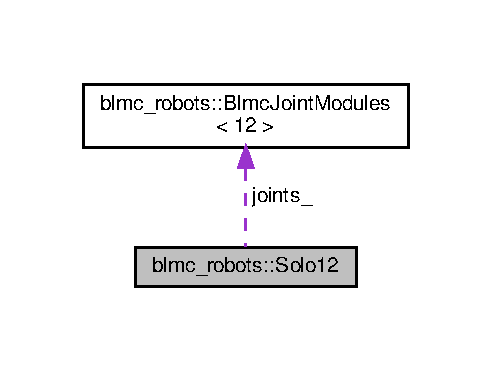
\includegraphics[width=236pt]{classblmc__robots_1_1Solo12__coll__graph}
\end{center}
\end{figure}
\subsection*{Public Member Functions}
\begin{DoxyCompactItemize}
\item 
\hyperlink{classblmc__robots_1_1Solo12_a9be95c29e80dca13a2dafa8a0f82eec5}{Solo12} ()
\begin{DoxyCompactList}\small\item\em Solo is the constructor of the class. \end{DoxyCompactList}\item 
void \hyperlink{classblmc__robots_1_1Solo12_ae3b1480bc12a079939b627950d55f66a}{initialize} (const std\+::string \&network\+\_\+id, const std\+::string \&serial\+\_\+port)
\begin{DoxyCompactList}\small\item\em Initialize the robot by setting aligning the motors and calibrate the sensors to 0. \end{DoxyCompactList}\item 
\mbox{\Hypertarget{classblmc__robots_1_1Solo12_a9f0d4a95fd4f82681f78dda1d519e5f9}\label{classblmc__robots_1_1Solo12_a9f0d4a95fd4f82681f78dda1d519e5f9}} 
void \hyperlink{classblmc__robots_1_1Solo12_a9f0d4a95fd4f82681f78dda1d519e5f9}{set\+\_\+max\+\_\+joint\+\_\+torques} (const double \&max\+\_\+joint\+\_\+torques)
\begin{DoxyCompactList}\small\item\em Sets the maximum joint torques. \end{DoxyCompactList}\item 
\mbox{\Hypertarget{classblmc__robots_1_1Solo12_a7f9bbd57bf8f0a9d54542c249c03fb47}\label{classblmc__robots_1_1Solo12_a7f9bbd57bf8f0a9d54542c249c03fb47}} 
void \hyperlink{classblmc__robots_1_1Solo12_a7f9bbd57bf8f0a9d54542c249c03fb47}{send\+\_\+target\+\_\+joint\+\_\+torque} (const Eigen\+::\+Ref$<$ \hyperlink{common__header_8hpp_a80313eb420184518596e745eecf4b494}{Vector12d} $>$ target\+\_\+joint\+\_\+torque)
\begin{DoxyCompactList}\small\item\em send\+\_\+target\+\_\+torques sends the target currents to the motors. \end{DoxyCompactList}\item 
void \hyperlink{classblmc__robots_1_1Solo12_aad9581cdcb139a49dbfb4673f18f7968}{acquire\+\_\+sensors} ()
\begin{DoxyCompactList}\small\item\em acquire\+\_\+sensors acquire all available sensors, W\+A\+R\+N\+I\+NG !!!! this method has to be called prior to any getter to have up to date data. \end{DoxyCompactList}\item 
bool \hyperlink{classblmc__robots_1_1Solo12_a8b9bfe0950a5d54ea5528aa98204f651}{calibrate} (const \hyperlink{common__header_8hpp_a80313eb420184518596e745eecf4b494}{Vector12d} \&home\+\_\+offset\+\_\+rad)
\begin{DoxyCompactList}\small\item\em Calibrate the joints by moving to the next joint index position. \end{DoxyCompactList}\item 
const Eigen\+::\+Ref$<$ \hyperlink{common__header_8hpp_a80313eb420184518596e745eecf4b494}{Vector12d} $>$ \hyperlink{classblmc__robots_1_1Solo12_a9ce8856916fb841f127be1920d18fea9}{get\+\_\+motor\+\_\+inertias} ()
\begin{DoxyCompactList}\small\item\em Joint properties. \end{DoxyCompactList}\item 
const Eigen\+::\+Ref$<$ \hyperlink{common__header_8hpp_a80313eb420184518596e745eecf4b494}{Vector12d} $>$ \hyperlink{classblmc__robots_1_1Solo12_a2135c79bff566dc0f8bace78bcf0b714}{get\+\_\+motor\+\_\+torque\+\_\+constants} ()
\begin{DoxyCompactList}\small\item\em get\+\_\+motor\+\_\+torque\+\_\+constants in \mbox{[}\mbox{]} \end{DoxyCompactList}\item 
const Eigen\+::\+Ref$<$ \hyperlink{common__header_8hpp_a80313eb420184518596e745eecf4b494}{Vector12d} $>$ \hyperlink{classblmc__robots_1_1Solo12_ab24a09564c336625a945523a74f91112}{get\+\_\+joint\+\_\+gear\+\_\+ratios} ()
\begin{DoxyCompactList}\small\item\em get\+\_\+joint\+\_\+gear\+\_\+ratios \end{DoxyCompactList}\item 
const Eigen\+::\+Ref$<$ \hyperlink{common__header_8hpp_a80313eb420184518596e745eecf4b494}{Vector12d} $>$ \hyperlink{classblmc__robots_1_1Solo12_aa1994a07d52a00275e0c85f0ad38fb12}{get\+\_\+motor\+\_\+max\+\_\+current} ()
\begin{DoxyCompactList}\small\item\em get\+\_\+max\+\_\+torque \end{DoxyCompactList}\item 
const Eigen\+::\+Ref$<$ \hyperlink{common__header_8hpp_a80313eb420184518596e745eecf4b494}{Vector12d} $>$ \hyperlink{classblmc__robots_1_1Solo12_a6ce3b791bba7cc37621a63ee6447c9c0}{get\+\_\+joint\+\_\+positions} ()
\begin{DoxyCompactList}\small\item\em Sensor Data. \end{DoxyCompactList}\item 
const Eigen\+::\+Ref$<$ \hyperlink{common__header_8hpp_a80313eb420184518596e745eecf4b494}{Vector12d} $>$ \hyperlink{classblmc__robots_1_1Solo12_aa0a6eb846038b644b425c1efd4c8a81f}{get\+\_\+joint\+\_\+velocities} ()
\begin{DoxyCompactList}\small\item\em get\+\_\+joint\+\_\+velocities \end{DoxyCompactList}\item 
const Eigen\+::\+Ref$<$ \hyperlink{common__header_8hpp_a80313eb420184518596e745eecf4b494}{Vector12d} $>$ \hyperlink{classblmc__robots_1_1Solo12_acfc399c1070c44d4ae98a1d806dca783}{get\+\_\+joint\+\_\+torques} ()
\begin{DoxyCompactList}\small\item\em get\+\_\+joint\+\_\+torques \end{DoxyCompactList}\item 
const Eigen\+::\+Ref$<$ \hyperlink{common__header_8hpp_a80313eb420184518596e745eecf4b494}{Vector12d} $>$ \hyperlink{classblmc__robots_1_1Solo12_ab8a6277bddcd64ec33eb8720d9478f7d}{get\+\_\+joint\+\_\+target\+\_\+torques} ()
\begin{DoxyCompactList}\small\item\em get\+\_\+joint\+\_\+torques \end{DoxyCompactList}\item 
const Eigen\+::\+Ref$<$ \hyperlink{common__header_8hpp_a80313eb420184518596e745eecf4b494}{Vector12d} $>$ \hyperlink{classblmc__robots_1_1Solo12_a7569444864f60d87ba9d9d0b5cc01afe}{get\+\_\+joint\+\_\+encoder\+\_\+index} ()
\begin{DoxyCompactList}\small\item\em get\+\_\+joint\+\_\+encoder\+\_\+index \end{DoxyCompactList}\item 
const Eigen\+::\+Ref$<$ Eigen\+::\+Vector4d $>$ \hyperlink{classblmc__robots_1_1Solo12_a79d74e1bbae286d8d79a94e328d3ad00}{get\+\_\+contact\+\_\+sensors\+\_\+states} ()
\begin{DoxyCompactList}\small\item\em get\+\_\+contact\+\_\+sensors\+\_\+states \end{DoxyCompactList}\item 
const Eigen\+::\+Ref$<$ Eigen\+::\+Vector4d $>$ \hyperlink{classblmc__robots_1_1Solo12_a2881a38d56aece096ca2c0ca42f2d56c}{get\+\_\+slider\+\_\+positions} ()
\begin{DoxyCompactList}\small\item\em get\+\_\+slider\+\_\+positions \end{DoxyCompactList}\item 
const std\+::array$<$ bool, 12 $>$ \& \hyperlink{classblmc__robots_1_1Solo12_a079e0ab1f33cb8e6cae03a85f58e8c4f}{get\+\_\+motor\+\_\+enabled} ()
\begin{DoxyCompactList}\small\item\em Hardware Status. \end{DoxyCompactList}\item 
const std\+::array$<$ bool, 12 $>$ \& \hyperlink{classblmc__robots_1_1Solo12_a37584471402cef8cf854d69bdbac98eb}{get\+\_\+motor\+\_\+ready} ()
\begin{DoxyCompactList}\small\item\em get\+\_\+motor\+\_\+ready \end{DoxyCompactList}\item 
const std\+::array$<$ bool, 6 $>$ \& \hyperlink{classblmc__robots_1_1Solo12_af9265895ea76870eeeec913cb6794806}{get\+\_\+motor\+\_\+board\+\_\+enabled} ()
\begin{DoxyCompactList}\small\item\em get\+\_\+motor\+\_\+board\+\_\+enabled \end{DoxyCompactList}\item 
const std\+::array$<$ int, 6 $>$ \& \hyperlink{classblmc__robots_1_1Solo12_aac115dccae0a43c10ace81a348f86182}{get\+\_\+motor\+\_\+board\+\_\+errors} ()
\begin{DoxyCompactList}\small\item\em get\+\_\+motor\+\_\+board\+\_\+errors \end{DoxyCompactList}\item 
bool \hyperlink{classblmc__robots_1_1Solo12_af8d51ec7885dab9c017aec9dd11937ad}{has\+\_\+error} () const
\begin{DoxyCompactList}\small\item\em has\+\_\+error \end{DoxyCompactList}\end{DoxyCompactItemize}
\subsection*{Private Attributes}
\begin{DoxyCompactItemize}
\item 
\hyperlink{common__header_8hpp_a80313eb420184518596e745eecf4b494}{Vector12d} \hyperlink{classblmc__robots_1_1Solo12_a625a9e4fe0be2fcad91a670d12f18bf3}{motor\+\_\+inertias\+\_\+}
\begin{DoxyCompactList}\small\item\em Joint properties. \end{DoxyCompactList}\item 
\hyperlink{common__header_8hpp_a80313eb420184518596e745eecf4b494}{Vector12d} \hyperlink{classblmc__robots_1_1Solo12_a4bab49dbf3f7234b6e0d5166696c885a}{motor\+\_\+torque\+\_\+constants\+\_\+}
\begin{DoxyCompactList}\small\item\em D\+CM motor torque constants. \end{DoxyCompactList}\item 
\hyperlink{common__header_8hpp_a80313eb420184518596e745eecf4b494}{Vector12d} \hyperlink{classblmc__robots_1_1Solo12_a03d025b7fa51624e1de5865340429b9f}{joint\+\_\+gear\+\_\+ratios\+\_\+}
\begin{DoxyCompactList}\small\item\em joint gear ratios (9). \end{DoxyCompactList}\item 
\hyperlink{common__header_8hpp_a80313eb420184518596e745eecf4b494}{Vector12d} \hyperlink{classblmc__robots_1_1Solo12_a46cab41a223dc4ee824e6d192cc01f9d}{motor\+\_\+max\+\_\+current\+\_\+}
\begin{DoxyCompactList}\small\item\em Max appliable current before the robot shutdown. \end{DoxyCompactList}\item 
\hyperlink{common__header_8hpp_a80313eb420184518596e745eecf4b494}{Vector12d} \hyperlink{classblmc__robots_1_1Solo12_ad3d4f55c1a8d5c16aaacf5e870370f18}{joint\+\_\+zero\+\_\+positions\+\_\+}
\begin{DoxyCompactList}\small\item\em Offset to the theoretical \char`\"{}0\char`\"{} pose. \end{DoxyCompactList}\item 
\mbox{\Hypertarget{classblmc__robots_1_1Solo12_a8eab2e983bfe76eafbcf054c385340a3}\label{classblmc__robots_1_1Solo12_a8eab2e983bfe76eafbcf054c385340a3}} 
Eigen\+::\+Array$<$ double, 12, 1 $>$ \hyperlink{classblmc__robots_1_1Solo12_a8eab2e983bfe76eafbcf054c385340a3}{max\+\_\+joint\+\_\+torques\+\_\+}
\begin{DoxyCompactList}\small\item\em Max joint torques (Nm) \end{DoxyCompactList}\item 
std\+::array$<$ bool, 12 $>$ \hyperlink{classblmc__robots_1_1Solo12_a50b6c097724e01436424b1f1c8dd0dd2}{motor\+\_\+enabled\+\_\+}
\begin{DoxyCompactList}\small\item\em 

 Hardware status \end{DoxyCompactList}\item 
\mbox{\Hypertarget{classblmc__robots_1_1Solo12_a653320521b1f1833edf592b5f89cc3a8}\label{classblmc__robots_1_1Solo12_a653320521b1f1833edf592b5f89cc3a8}} 
std\+::array$<$ bool, 12 $>$ \hyperlink{classblmc__robots_1_1Solo12_a653320521b1f1833edf592b5f89cc3a8}{motor\+\_\+ready\+\_\+}
\begin{DoxyCompactList}\small\item\em This gives the status (enabled/disabled) of each motors using the joint ordering convention. \end{DoxyCompactList}\item 
\mbox{\Hypertarget{classblmc__robots_1_1Solo12_a33269cf4037c0a3812fe8127dcf65976}\label{classblmc__robots_1_1Solo12_a33269cf4037c0a3812fe8127dcf65976}} 
std\+::array$<$ bool, 6 $>$ \hyperlink{classblmc__robots_1_1Solo12_a33269cf4037c0a3812fe8127dcf65976}{motor\+\_\+board\+\_\+enabled\+\_\+}
\begin{DoxyCompactList}\small\item\em This gives the status (enabled/disabled of the onboard control cards). \end{DoxyCompactList}\item 
\mbox{\Hypertarget{classblmc__robots_1_1Solo12_af08cfab9b12464b12d2991c0b3376631}\label{classblmc__robots_1_1Solo12_af08cfab9b12464b12d2991c0b3376631}} 
std\+::array$<$ int, 6 $>$ \hyperlink{classblmc__robots_1_1Solo12_af08cfab9b12464b12d2991c0b3376631}{motor\+\_\+board\+\_\+errors\+\_\+}
\begin{DoxyCompactList}\small\item\em This gives the status (enabled/disabled of the onboard control cards). \end{DoxyCompactList}\item 
\hyperlink{common__header_8hpp_a80313eb420184518596e745eecf4b494}{Vector12d} \hyperlink{classblmc__robots_1_1Solo12_a30531d872c6de968876110416ce777a9}{joint\+\_\+positions\+\_\+}
\begin{DoxyCompactList}\small\item\em Joint data. \end{DoxyCompactList}\item 
\mbox{\Hypertarget{classblmc__robots_1_1Solo12_af9b0cbb28848b50a3706316991d34cca}\label{classblmc__robots_1_1Solo12_af9b0cbb28848b50a3706316991d34cca}} 
\hyperlink{common__header_8hpp_a80313eb420184518596e745eecf4b494}{Vector12d} \hyperlink{classblmc__robots_1_1Solo12_af9b0cbb28848b50a3706316991d34cca}{joint\+\_\+velocities\+\_\+}
\begin{DoxyCompactList}\small\item\em joint\+\_\+velocities\+\_\+ \end{DoxyCompactList}\item 
\mbox{\Hypertarget{classblmc__robots_1_1Solo12_a515270deaf070b4369b2863872868058}\label{classblmc__robots_1_1Solo12_a515270deaf070b4369b2863872868058}} 
\hyperlink{common__header_8hpp_a80313eb420184518596e745eecf4b494}{Vector12d} \hyperlink{classblmc__robots_1_1Solo12_a515270deaf070b4369b2863872868058}{joint\+\_\+torques\+\_\+}
\begin{DoxyCompactList}\small\item\em joint\+\_\+torques\+\_\+ \end{DoxyCompactList}\item 
\mbox{\Hypertarget{classblmc__robots_1_1Solo12_a8243cd85b37980e512f43f8da79ab080}\label{classblmc__robots_1_1Solo12_a8243cd85b37980e512f43f8da79ab080}} 
\hyperlink{common__header_8hpp_a80313eb420184518596e745eecf4b494}{Vector12d} \hyperlink{classblmc__robots_1_1Solo12_a8243cd85b37980e512f43f8da79ab080}{joint\+\_\+target\+\_\+torques\+\_\+}
\begin{DoxyCompactList}\small\item\em joint\+\_\+target\+\_\+torques\+\_\+ \end{DoxyCompactList}\item 
\mbox{\Hypertarget{classblmc__robots_1_1Solo12_a9e9743d8043db4b0a64fb914bda53714}\label{classblmc__robots_1_1Solo12_a9e9743d8043db4b0a64fb914bda53714}} 
\hyperlink{common__header_8hpp_a80313eb420184518596e745eecf4b494}{Vector12d} \hyperlink{classblmc__robots_1_1Solo12_a9e9743d8043db4b0a64fb914bda53714}{joint\+\_\+encoder\+\_\+index\+\_\+}
\begin{DoxyCompactList}\small\item\em joint\+\_\+encoder\+\_\+index\+\_\+ \end{DoxyCompactList}\item 
Eigen\+::\+Vector4d \hyperlink{classblmc__robots_1_1Solo12_a67948750642c1e62f4aeadb4adac3bdd}{slider\+\_\+positions\+\_\+}
\begin{DoxyCompactList}\small\item\em 

 Additional data \end{DoxyCompactList}\item 
\mbox{\Hypertarget{classblmc__robots_1_1Solo12_a0d9feba0ec7b4b34e463f85e778dc171}\label{classblmc__robots_1_1Solo12_a0d9feba0ec7b4b34e463f85e778dc171}} 
std\+::vector$<$ int $>$ \hyperlink{classblmc__robots_1_1Solo12_a0d9feba0ec7b4b34e463f85e778dc171}{slider\+\_\+positions\+\_\+vector\+\_\+}
\begin{DoxyCompactList}\small\item\em For reading the raw slider values from the serial port. \end{DoxyCompactList}\item 
\mbox{\Hypertarget{classblmc__robots_1_1Solo12_a04c43e0f8862e97e7902419edb7cd2a2}\label{classblmc__robots_1_1Solo12_a04c43e0f8862e97e7902419edb7cd2a2}} 
Eigen\+::\+Vector4d \hyperlink{classblmc__robots_1_1Solo12_a04c43e0f8862e97e7902419edb7cd2a2}{contact\+\_\+sensors\+\_\+states\+\_\+}
\begin{DoxyCompactList}\small\item\em contact\+\_\+sensors\+\_\+ is contact sensors at each feet of teh quadruped. \end{DoxyCompactList}\item 
\mbox{\Hypertarget{classblmc__robots_1_1Solo12_aa2fe5722e58645d80641238d1563b371}\label{classblmc__robots_1_1Solo12_aa2fe5722e58645d80641238d1563b371}} 
std\+::string \hyperlink{classblmc__robots_1_1Solo12_aa2fe5722e58645d80641238d1563b371}{network\+\_\+id\+\_\+}
\begin{DoxyCompactList}\small\item\em This is the name of the network\+: Left column in ifconfig output. \end{DoxyCompactList}\item 
std\+::array$<$ int, 12 $>$ \hyperlink{classblmc__robots_1_1Solo12_a783154ba0e9e7a931bc25a2ae17cea37}{map\+\_\+joint\+\_\+id\+\_\+to\+\_\+motor\+\_\+board\+\_\+id\+\_\+}
\begin{DoxyCompactList}\small\item\em Map the joint id to the motor board id,. \end{DoxyCompactList}\item 
std\+::array$<$ int, 12 $>$ \hyperlink{classblmc__robots_1_1Solo12_adc6fc34d0685db1e9a6094474d1db903}{map\+\_\+joint\+\_\+id\+\_\+to\+\_\+motor\+\_\+port\+\_\+id\+\_\+}
\begin{DoxyCompactList}\small\item\em Map the joint id to the motor port id,. \end{DoxyCompactList}\item 
std\+::shared\+\_\+ptr$<$ Master\+Board\+Interface $>$ \hyperlink{classblmc__robots_1_1Solo12_a2675d6567258d0f02d387e228a6e85e1}{main\+\_\+board\+\_\+ptr\+\_\+}
\begin{DoxyCompactList}\small\item\em Drivers communication objects. \end{DoxyCompactList}\item 
std\+::shared\+\_\+ptr$<$ blmc\+\_\+drivers\+::\+Spi\+Bus $>$ \hyperlink{classblmc__robots_1_1Solo12_a416708664f404b0d140e02fe8b90bd00}{spi\+\_\+bus\+\_\+}
\begin{DoxyCompactList}\small\item\em Main board blmc\+\_\+drivers overlay. \end{DoxyCompactList}\item 
\mbox{\Hypertarget{classblmc__robots_1_1Solo12_a640f378577e818ae36f96145760edd65}\label{classblmc__robots_1_1Solo12_a640f378577e818ae36f96145760edd65}} 
std\+::shared\+\_\+ptr$<$ blmc\+\_\+drivers\+::\+Serial\+Reader $>$ \hyperlink{classblmc__robots_1_1Solo12_a640f378577e818ae36f96145760edd65}{serial\+\_\+reader\+\_\+}
\begin{DoxyCompactList}\small\item\em Reader for serial port to read arduino slider values. \end{DoxyCompactList}\item 
std\+::array$<$ std\+::shared\+\_\+ptr$<$ blmc\+\_\+drivers\+::\+Spi\+Motor\+Board $>$, 6 $>$ \hyperlink{classblmc__robots_1_1Solo12_a84c520852a2ebd410eff9795e37473b3}{motor\+\_\+boards\+\_\+}
\begin{DoxyCompactList}\small\item\em These are the 6 motor boards of the robot. \end{DoxyCompactList}\item 
std\+::array$<$ \hyperlink{common__header_8hpp_ae1a0f9992bc8fbbc1943d887f517c180}{Motor\+Interface\+\_\+ptr}, 12 $>$ \hyperlink{classblmc__robots_1_1Solo12_a91e6592fb8a24aabb9a9795cccc130cf}{motors\+\_\+}
\begin{DoxyCompactList}\small\item\em motors\+\_\+ are the objects allowing us to send motor commands and receive data. \end{DoxyCompactList}\item 
std\+::array$<$ \hyperlink{common__header_8hpp_a4cb9a95e8b2c0bf237ce29f5252c7b73}{Slider\+\_\+ptr}, 4 $>$ \hyperlink{classblmc__robots_1_1Solo12_a4119af8c0b732d5559f8d71a9714ac29}{sliders\+\_\+}
\begin{DoxyCompactList}\small\item\em sliders\+\_\+ these are analogue input, typically from linear potentiometers. \end{DoxyCompactList}\item 
\mbox{\Hypertarget{classblmc__robots_1_1Solo12_a1949ee20f0762be56a0020af1cf5727a}\label{classblmc__robots_1_1Solo12_a1949ee20f0762be56a0020af1cf5727a}} 
\hyperlink{classblmc__robots_1_1BlmcJointModules}{Blmc\+Joint\+Modules}$<$ 12 $>$ \hyperlink{classblmc__robots_1_1Solo12_a1949ee20f0762be56a0020af1cf5727a}{joints\+\_\+}
\begin{DoxyCompactList}\small\item\em Joint modules containing the driving system paramters. \end{DoxyCompactList}\item 
std\+::array$<$ bool, 12 $>$ \hyperlink{classblmc__robots_1_1Solo12_ace2b1af72676f4ec2d285f6166ba6922}{reverse\+\_\+polarities\+\_\+}
\begin{DoxyCompactList}\small\item\em Address the rotation direction of the motor. \end{DoxyCompactList}\item 
bool \hyperlink{classblmc__robots_1_1Solo12_a9e28ceac427c283b4e66a1bde15baed8}{active\+\_\+estop\+\_\+}
\begin{DoxyCompactList}\small\item\em If the physical estop is pressed or not. \end{DoxyCompactList}\end{DoxyCompactItemize}
\subsection*{Static Private Attributes}
\begin{DoxyCompactItemize}
\item 
static const double \hyperlink{classblmc__robots_1_1Solo12_a7e83448a46ffc61cc70e4b82883ee113}{max\+\_\+joint\+\_\+torque\+\_\+security\+\_\+margin\+\_\+} = 0.\+99
\begin{DoxyCompactList}\small\item\em Security margin on the saturation of the control. \end{DoxyCompactList}\end{DoxyCompactItemize}


\subsection{Detailed Description}
Definition and drivers for the \hyperlink{classblmc__robots_1_1Solo12}{Solo12} robot. 

Mapping between the D\+OF and driver boards + motor ports\+: F\+L\+\_\+\+H\+AA -\/ motor board 0, motor port 0, motor index 0 F\+L\+\_\+\+H\+FE -\/ motor board 1, motor port 1, motor index 3 F\+L\+\_\+\+K\+FE -\/ motor board 1, motor port 0, motor index 2 F\+R\+\_\+\+H\+AA -\/ motor board 0, motor port 1, motor index 1 F\+R\+\_\+\+H\+FE -\/ motor board 2, motor port 1, motor index 5 F\+R\+\_\+\+K\+FE -\/ motor board 2, motor port 0, motor index 4 H\+L\+\_\+\+H\+AA -\/ motor board 3, motor port 0, motor index 6 H\+L\+\_\+\+H\+FE -\/ motor board 4, motor port 1, motor index 9 H\+L\+\_\+\+K\+FE -\/ motor board 4, motor port 0, motor index 8 H\+R\+\_\+\+H\+AA -\/ motor board 3, motor port 1, motor index 7 H\+R\+\_\+\+H\+FE -\/ motor board 5, motor port 1, motor index 11 H\+R\+\_\+\+K\+FE -\/ motor board 5, motor port 0, motor index 10 

\subsection{Constructor \& Destructor Documentation}
\mbox{\Hypertarget{classblmc__robots_1_1Solo12_a9be95c29e80dca13a2dafa8a0f82eec5}\label{classblmc__robots_1_1Solo12_a9be95c29e80dca13a2dafa8a0f82eec5}} 
\index{blmc\+\_\+robots\+::\+Solo12@{blmc\+\_\+robots\+::\+Solo12}!Solo12@{Solo12}}
\index{Solo12@{Solo12}!blmc\+\_\+robots\+::\+Solo12@{blmc\+\_\+robots\+::\+Solo12}}
\subsubsection{\texorpdfstring{Solo12()}{Solo12()}}
{\footnotesize\ttfamily blmc\+\_\+robots\+::\+Solo12\+::\+Solo12 (\begin{DoxyParamCaption}{ }\end{DoxyParamCaption})}



Solo is the constructor of the class. 

Hardware properties

Hardware status

Joint data

Additional data

Setup some known data

\subsection{Member Function Documentation}
\mbox{\Hypertarget{classblmc__robots_1_1Solo12_aad9581cdcb139a49dbfb4673f18f7968}\label{classblmc__robots_1_1Solo12_aad9581cdcb139a49dbfb4673f18f7968}} 
\index{blmc\+\_\+robots\+::\+Solo12@{blmc\+\_\+robots\+::\+Solo12}!acquire\+\_\+sensors@{acquire\+\_\+sensors}}
\index{acquire\+\_\+sensors@{acquire\+\_\+sensors}!blmc\+\_\+robots\+::\+Solo12@{blmc\+\_\+robots\+::\+Solo12}}
\subsubsection{\texorpdfstring{acquire\+\_\+sensors()}{acquire\_sensors()}}
{\footnotesize\ttfamily void blmc\+\_\+robots\+::\+Solo12\+::acquire\+\_\+sensors (\begin{DoxyParamCaption}{ }\end{DoxyParamCaption})}



acquire\+\_\+sensors acquire all available sensors, W\+A\+R\+N\+I\+NG !!!! this method has to be called prior to any getter to have up to date data. 

Joint data

Additional data

The different status.\mbox{\Hypertarget{classblmc__robots_1_1Solo12_a8b9bfe0950a5d54ea5528aa98204f651}\label{classblmc__robots_1_1Solo12_a8b9bfe0950a5d54ea5528aa98204f651}} 
\index{blmc\+\_\+robots\+::\+Solo12@{blmc\+\_\+robots\+::\+Solo12}!calibrate@{calibrate}}
\index{calibrate@{calibrate}!blmc\+\_\+robots\+::\+Solo12@{blmc\+\_\+robots\+::\+Solo12}}
\subsubsection{\texorpdfstring{calibrate()}{calibrate()}}
{\footnotesize\ttfamily bool blmc\+\_\+robots\+::\+Solo12\+::calibrate (\begin{DoxyParamCaption}\item[{const \hyperlink{common__header_8hpp_a80313eb420184518596e745eecf4b494}{Vector12d} \&}]{home\+\_\+offset\+\_\+rad }\end{DoxyParamCaption})}



Calibrate the joints by moving to the next joint index position. 


\begin{DoxyParams}{Parameters}
{\em home\+\_\+offset\+\_\+rad} & This is the angle between the index and the zero pose. \\
\hline
\end{DoxyParams}
\begin{DoxyReturn}{Returns}
true in case of success. 

false in case of failure. 
\end{DoxyReturn}
\mbox{\Hypertarget{classblmc__robots_1_1Solo12_a79d74e1bbae286d8d79a94e328d3ad00}\label{classblmc__robots_1_1Solo12_a79d74e1bbae286d8d79a94e328d3ad00}} 
\index{blmc\+\_\+robots\+::\+Solo12@{blmc\+\_\+robots\+::\+Solo12}!get\+\_\+contact\+\_\+sensors\+\_\+states@{get\+\_\+contact\+\_\+sensors\+\_\+states}}
\index{get\+\_\+contact\+\_\+sensors\+\_\+states@{get\+\_\+contact\+\_\+sensors\+\_\+states}!blmc\+\_\+robots\+::\+Solo12@{blmc\+\_\+robots\+::\+Solo12}}
\subsubsection{\texorpdfstring{get\+\_\+contact\+\_\+sensors\+\_\+states()}{get\_contact\_sensors\_states()}}
{\footnotesize\ttfamily const Eigen\+::\+Ref$<$Eigen\+::\+Vector4d$>$ blmc\+\_\+robots\+::\+Solo12\+::get\+\_\+contact\+\_\+sensors\+\_\+states (\begin{DoxyParamCaption}{ }\end{DoxyParamCaption})\hspace{0.3cm}{\ttfamily [inline]}}



get\+\_\+contact\+\_\+sensors\+\_\+states 

\begin{DoxyReturn}{Returns}
the state of the contacts states W\+A\+R\+N\+I\+NG !!!! The method $<$acquire\+\_\+sensors$>$\char`\"{}()\char`\"{} has to be called prior to any getter to have up to date data. 
\end{DoxyReturn}
\mbox{\Hypertarget{classblmc__robots_1_1Solo12_a7569444864f60d87ba9d9d0b5cc01afe}\label{classblmc__robots_1_1Solo12_a7569444864f60d87ba9d9d0b5cc01afe}} 
\index{blmc\+\_\+robots\+::\+Solo12@{blmc\+\_\+robots\+::\+Solo12}!get\+\_\+joint\+\_\+encoder\+\_\+index@{get\+\_\+joint\+\_\+encoder\+\_\+index}}
\index{get\+\_\+joint\+\_\+encoder\+\_\+index@{get\+\_\+joint\+\_\+encoder\+\_\+index}!blmc\+\_\+robots\+::\+Solo12@{blmc\+\_\+robots\+::\+Solo12}}
\subsubsection{\texorpdfstring{get\+\_\+joint\+\_\+encoder\+\_\+index()}{get\_joint\_encoder\_index()}}
{\footnotesize\ttfamily const Eigen\+::\+Ref$<$\hyperlink{common__header_8hpp_a80313eb420184518596e745eecf4b494}{Vector12d}$>$ blmc\+\_\+robots\+::\+Solo12\+::get\+\_\+joint\+\_\+encoder\+\_\+index (\begin{DoxyParamCaption}{ }\end{DoxyParamCaption})\hspace{0.3cm}{\ttfamily [inline]}}



get\+\_\+joint\+\_\+encoder\+\_\+index 

\begin{DoxyReturn}{Returns}
the position of the index of the encoders a the motor level W\+A\+R\+N\+I\+NG !!!! The method $<$acquire\+\_\+sensors$>$\char`\"{}()\char`\"{} has to be called prior to any getter to have up to date data. 
\end{DoxyReturn}
\mbox{\Hypertarget{classblmc__robots_1_1Solo12_ab24a09564c336625a945523a74f91112}\label{classblmc__robots_1_1Solo12_ab24a09564c336625a945523a74f91112}} 
\index{blmc\+\_\+robots\+::\+Solo12@{blmc\+\_\+robots\+::\+Solo12}!get\+\_\+joint\+\_\+gear\+\_\+ratios@{get\+\_\+joint\+\_\+gear\+\_\+ratios}}
\index{get\+\_\+joint\+\_\+gear\+\_\+ratios@{get\+\_\+joint\+\_\+gear\+\_\+ratios}!blmc\+\_\+robots\+::\+Solo12@{blmc\+\_\+robots\+::\+Solo12}}
\subsubsection{\texorpdfstring{get\+\_\+joint\+\_\+gear\+\_\+ratios()}{get\_joint\_gear\_ratios()}}
{\footnotesize\ttfamily const Eigen\+::\+Ref$<$\hyperlink{common__header_8hpp_a80313eb420184518596e745eecf4b494}{Vector12d}$>$ blmc\+\_\+robots\+::\+Solo12\+::get\+\_\+joint\+\_\+gear\+\_\+ratios (\begin{DoxyParamCaption}{ }\end{DoxyParamCaption})\hspace{0.3cm}{\ttfamily [inline]}}



get\+\_\+joint\+\_\+gear\+\_\+ratios 

\begin{DoxyReturn}{Returns}
Joint gear ratios 
\end{DoxyReturn}
\mbox{\Hypertarget{classblmc__robots_1_1Solo12_a6ce3b791bba7cc37621a63ee6447c9c0}\label{classblmc__robots_1_1Solo12_a6ce3b791bba7cc37621a63ee6447c9c0}} 
\index{blmc\+\_\+robots\+::\+Solo12@{blmc\+\_\+robots\+::\+Solo12}!get\+\_\+joint\+\_\+positions@{get\+\_\+joint\+\_\+positions}}
\index{get\+\_\+joint\+\_\+positions@{get\+\_\+joint\+\_\+positions}!blmc\+\_\+robots\+::\+Solo12@{blmc\+\_\+robots\+::\+Solo12}}
\subsubsection{\texorpdfstring{get\+\_\+joint\+\_\+positions()}{get\_joint\_positions()}}
{\footnotesize\ttfamily const Eigen\+::\+Ref$<$\hyperlink{common__header_8hpp_a80313eb420184518596e745eecf4b494}{Vector12d}$>$ blmc\+\_\+robots\+::\+Solo12\+::get\+\_\+joint\+\_\+positions (\begin{DoxyParamCaption}{ }\end{DoxyParamCaption})\hspace{0.3cm}{\ttfamily [inline]}}



Sensor Data. 

get\+\_\+joint\+\_\+positions \begin{DoxyReturn}{Returns}
the joint angle of each module W\+A\+R\+N\+I\+NG !!!! The method $<$acquire\+\_\+sensors$>$\char`\"{}()\char`\"{} has to be called prior to any getter to have up to date data. 
\end{DoxyReturn}
\mbox{\Hypertarget{classblmc__robots_1_1Solo12_ab8a6277bddcd64ec33eb8720d9478f7d}\label{classblmc__robots_1_1Solo12_ab8a6277bddcd64ec33eb8720d9478f7d}} 
\index{blmc\+\_\+robots\+::\+Solo12@{blmc\+\_\+robots\+::\+Solo12}!get\+\_\+joint\+\_\+target\+\_\+torques@{get\+\_\+joint\+\_\+target\+\_\+torques}}
\index{get\+\_\+joint\+\_\+target\+\_\+torques@{get\+\_\+joint\+\_\+target\+\_\+torques}!blmc\+\_\+robots\+::\+Solo12@{blmc\+\_\+robots\+::\+Solo12}}
\subsubsection{\texorpdfstring{get\+\_\+joint\+\_\+target\+\_\+torques()}{get\_joint\_target\_torques()}}
{\footnotesize\ttfamily const Eigen\+::\+Ref$<$\hyperlink{common__header_8hpp_a80313eb420184518596e745eecf4b494}{Vector12d}$>$ blmc\+\_\+robots\+::\+Solo12\+::get\+\_\+joint\+\_\+target\+\_\+torques (\begin{DoxyParamCaption}{ }\end{DoxyParamCaption})\hspace{0.3cm}{\ttfamily [inline]}}



get\+\_\+joint\+\_\+torques 

\begin{DoxyReturn}{Returns}
the target joint torques W\+A\+R\+N\+I\+NG !!!! The method $<$acquire\+\_\+sensors$>$\char`\"{}()\char`\"{} has to be called prior to any getter to have up to date data. 
\end{DoxyReturn}
\mbox{\Hypertarget{classblmc__robots_1_1Solo12_acfc399c1070c44d4ae98a1d806dca783}\label{classblmc__robots_1_1Solo12_acfc399c1070c44d4ae98a1d806dca783}} 
\index{blmc\+\_\+robots\+::\+Solo12@{blmc\+\_\+robots\+::\+Solo12}!get\+\_\+joint\+\_\+torques@{get\+\_\+joint\+\_\+torques}}
\index{get\+\_\+joint\+\_\+torques@{get\+\_\+joint\+\_\+torques}!blmc\+\_\+robots\+::\+Solo12@{blmc\+\_\+robots\+::\+Solo12}}
\subsubsection{\texorpdfstring{get\+\_\+joint\+\_\+torques()}{get\_joint\_torques()}}
{\footnotesize\ttfamily const Eigen\+::\+Ref$<$\hyperlink{common__header_8hpp_a80313eb420184518596e745eecf4b494}{Vector12d}$>$ blmc\+\_\+robots\+::\+Solo12\+::get\+\_\+joint\+\_\+torques (\begin{DoxyParamCaption}{ }\end{DoxyParamCaption})\hspace{0.3cm}{\ttfamily [inline]}}



get\+\_\+joint\+\_\+torques 

\begin{DoxyReturn}{Returns}
the joint torques W\+A\+R\+N\+I\+NG !!!! The method $<$acquire\+\_\+sensors$>$\char`\"{}()\char`\"{} has to be called prior to any getter to have up to date data. 
\end{DoxyReturn}
\mbox{\Hypertarget{classblmc__robots_1_1Solo12_aa0a6eb846038b644b425c1efd4c8a81f}\label{classblmc__robots_1_1Solo12_aa0a6eb846038b644b425c1efd4c8a81f}} 
\index{blmc\+\_\+robots\+::\+Solo12@{blmc\+\_\+robots\+::\+Solo12}!get\+\_\+joint\+\_\+velocities@{get\+\_\+joint\+\_\+velocities}}
\index{get\+\_\+joint\+\_\+velocities@{get\+\_\+joint\+\_\+velocities}!blmc\+\_\+robots\+::\+Solo12@{blmc\+\_\+robots\+::\+Solo12}}
\subsubsection{\texorpdfstring{get\+\_\+joint\+\_\+velocities()}{get\_joint\_velocities()}}
{\footnotesize\ttfamily const Eigen\+::\+Ref$<$\hyperlink{common__header_8hpp_a80313eb420184518596e745eecf4b494}{Vector12d}$>$ blmc\+\_\+robots\+::\+Solo12\+::get\+\_\+joint\+\_\+velocities (\begin{DoxyParamCaption}{ }\end{DoxyParamCaption})\hspace{0.3cm}{\ttfamily [inline]}}



get\+\_\+joint\+\_\+velocities 

\begin{DoxyReturn}{Returns}
the joint velocities W\+A\+R\+N\+I\+NG !!!! The method $<$acquire\+\_\+sensors$>$\char`\"{}()\char`\"{} has to be called prior to any getter to have up to date data. 
\end{DoxyReturn}
\mbox{\Hypertarget{classblmc__robots_1_1Solo12_af9265895ea76870eeeec913cb6794806}\label{classblmc__robots_1_1Solo12_af9265895ea76870eeeec913cb6794806}} 
\index{blmc\+\_\+robots\+::\+Solo12@{blmc\+\_\+robots\+::\+Solo12}!get\+\_\+motor\+\_\+board\+\_\+enabled@{get\+\_\+motor\+\_\+board\+\_\+enabled}}
\index{get\+\_\+motor\+\_\+board\+\_\+enabled@{get\+\_\+motor\+\_\+board\+\_\+enabled}!blmc\+\_\+robots\+::\+Solo12@{blmc\+\_\+robots\+::\+Solo12}}
\subsubsection{\texorpdfstring{get\+\_\+motor\+\_\+board\+\_\+enabled()}{get\_motor\_board\_enabled()}}
{\footnotesize\ttfamily const std\+::array$<$bool, 6$>$\& blmc\+\_\+robots\+::\+Solo12\+::get\+\_\+motor\+\_\+board\+\_\+enabled (\begin{DoxyParamCaption}{ }\end{DoxyParamCaption})\hspace{0.3cm}{\ttfamily [inline]}}



get\+\_\+motor\+\_\+board\+\_\+enabled 

\begin{DoxyReturn}{Returns}
This gives the status (enabled/disabled of the onboard control cards). 
\end{DoxyReturn}
\mbox{\Hypertarget{classblmc__robots_1_1Solo12_aac115dccae0a43c10ace81a348f86182}\label{classblmc__robots_1_1Solo12_aac115dccae0a43c10ace81a348f86182}} 
\index{blmc\+\_\+robots\+::\+Solo12@{blmc\+\_\+robots\+::\+Solo12}!get\+\_\+motor\+\_\+board\+\_\+errors@{get\+\_\+motor\+\_\+board\+\_\+errors}}
\index{get\+\_\+motor\+\_\+board\+\_\+errors@{get\+\_\+motor\+\_\+board\+\_\+errors}!blmc\+\_\+robots\+::\+Solo12@{blmc\+\_\+robots\+::\+Solo12}}
\subsubsection{\texorpdfstring{get\+\_\+motor\+\_\+board\+\_\+errors()}{get\_motor\_board\_errors()}}
{\footnotesize\ttfamily const std\+::array$<$int, 6$>$\& blmc\+\_\+robots\+::\+Solo12\+::get\+\_\+motor\+\_\+board\+\_\+errors (\begin{DoxyParamCaption}{ }\end{DoxyParamCaption})\hspace{0.3cm}{\ttfamily [inline]}}



get\+\_\+motor\+\_\+board\+\_\+errors 

\begin{DoxyReturn}{Returns}
This gives the status (enabled/disabled of the onboard control cards). 
\end{DoxyReturn}
\mbox{\Hypertarget{classblmc__robots_1_1Solo12_a079e0ab1f33cb8e6cae03a85f58e8c4f}\label{classblmc__robots_1_1Solo12_a079e0ab1f33cb8e6cae03a85f58e8c4f}} 
\index{blmc\+\_\+robots\+::\+Solo12@{blmc\+\_\+robots\+::\+Solo12}!get\+\_\+motor\+\_\+enabled@{get\+\_\+motor\+\_\+enabled}}
\index{get\+\_\+motor\+\_\+enabled@{get\+\_\+motor\+\_\+enabled}!blmc\+\_\+robots\+::\+Solo12@{blmc\+\_\+robots\+::\+Solo12}}
\subsubsection{\texorpdfstring{get\+\_\+motor\+\_\+enabled()}{get\_motor\_enabled()}}
{\footnotesize\ttfamily const std\+::array$<$bool, 12$>$\& blmc\+\_\+robots\+::\+Solo12\+::get\+\_\+motor\+\_\+enabled (\begin{DoxyParamCaption}{ }\end{DoxyParamCaption})\hspace{0.3cm}{\ttfamily [inline]}}



Hardware Status. 

get\+\_\+motor\+\_\+enabled \begin{DoxyReturn}{Returns}
This gives the status (enabled/disabled) of each motors using the joint ordering convention. 
\end{DoxyReturn}
\mbox{\Hypertarget{classblmc__robots_1_1Solo12_a9ce8856916fb841f127be1920d18fea9}\label{classblmc__robots_1_1Solo12_a9ce8856916fb841f127be1920d18fea9}} 
\index{blmc\+\_\+robots\+::\+Solo12@{blmc\+\_\+robots\+::\+Solo12}!get\+\_\+motor\+\_\+inertias@{get\+\_\+motor\+\_\+inertias}}
\index{get\+\_\+motor\+\_\+inertias@{get\+\_\+motor\+\_\+inertias}!blmc\+\_\+robots\+::\+Solo12@{blmc\+\_\+robots\+::\+Solo12}}
\subsubsection{\texorpdfstring{get\+\_\+motor\+\_\+inertias()}{get\_motor\_inertias()}}
{\footnotesize\ttfamily const Eigen\+::\+Ref$<$\hyperlink{common__header_8hpp_a80313eb420184518596e745eecf4b494}{Vector12d}$>$ blmc\+\_\+robots\+::\+Solo12\+::get\+\_\+motor\+\_\+inertias (\begin{DoxyParamCaption}{ }\end{DoxyParamCaption})\hspace{0.3cm}{\ttfamily [inline]}}



Joint properties. 

get\+\_\+motor\+\_\+inertias in \mbox{[}kg m$^\wedge$2\mbox{]} \begin{DoxyReturn}{Returns}
Motor inertias. 
\end{DoxyReturn}
\mbox{\Hypertarget{classblmc__robots_1_1Solo12_aa1994a07d52a00275e0c85f0ad38fb12}\label{classblmc__robots_1_1Solo12_aa1994a07d52a00275e0c85f0ad38fb12}} 
\index{blmc\+\_\+robots\+::\+Solo12@{blmc\+\_\+robots\+::\+Solo12}!get\+\_\+motor\+\_\+max\+\_\+current@{get\+\_\+motor\+\_\+max\+\_\+current}}
\index{get\+\_\+motor\+\_\+max\+\_\+current@{get\+\_\+motor\+\_\+max\+\_\+current}!blmc\+\_\+robots\+::\+Solo12@{blmc\+\_\+robots\+::\+Solo12}}
\subsubsection{\texorpdfstring{get\+\_\+motor\+\_\+max\+\_\+current()}{get\_motor\_max\_current()}}
{\footnotesize\ttfamily const Eigen\+::\+Ref$<$\hyperlink{common__header_8hpp_a80313eb420184518596e745eecf4b494}{Vector12d}$>$ blmc\+\_\+robots\+::\+Solo12\+::get\+\_\+motor\+\_\+max\+\_\+current (\begin{DoxyParamCaption}{ }\end{DoxyParamCaption})\hspace{0.3cm}{\ttfamily [inline]}}



get\+\_\+max\+\_\+torque 

\begin{DoxyReturn}{Returns}
the max torque that has been hardcoded in the constructor of this class.
\end{DoxyReturn}
\begin{DoxyRefDesc}{Todo}
\item[\hyperlink{todo__todo000001}{Todo}]Parametrize the maximum current via yaml or something else. \end{DoxyRefDesc}
\mbox{\Hypertarget{classblmc__robots_1_1Solo12_a37584471402cef8cf854d69bdbac98eb}\label{classblmc__robots_1_1Solo12_a37584471402cef8cf854d69bdbac98eb}} 
\index{blmc\+\_\+robots\+::\+Solo12@{blmc\+\_\+robots\+::\+Solo12}!get\+\_\+motor\+\_\+ready@{get\+\_\+motor\+\_\+ready}}
\index{get\+\_\+motor\+\_\+ready@{get\+\_\+motor\+\_\+ready}!blmc\+\_\+robots\+::\+Solo12@{blmc\+\_\+robots\+::\+Solo12}}
\subsubsection{\texorpdfstring{get\+\_\+motor\+\_\+ready()}{get\_motor\_ready()}}
{\footnotesize\ttfamily const std\+::array$<$bool, 12$>$\& blmc\+\_\+robots\+::\+Solo12\+::get\+\_\+motor\+\_\+ready (\begin{DoxyParamCaption}{ }\end{DoxyParamCaption})\hspace{0.3cm}{\ttfamily [inline]}}



get\+\_\+motor\+\_\+ready 

\begin{DoxyReturn}{Returns}
This gives the status (enabled/disabled) of each motors using the joint ordering convention. 
\end{DoxyReturn}
\mbox{\Hypertarget{classblmc__robots_1_1Solo12_a2135c79bff566dc0f8bace78bcf0b714}\label{classblmc__robots_1_1Solo12_a2135c79bff566dc0f8bace78bcf0b714}} 
\index{blmc\+\_\+robots\+::\+Solo12@{blmc\+\_\+robots\+::\+Solo12}!get\+\_\+motor\+\_\+torque\+\_\+constants@{get\+\_\+motor\+\_\+torque\+\_\+constants}}
\index{get\+\_\+motor\+\_\+torque\+\_\+constants@{get\+\_\+motor\+\_\+torque\+\_\+constants}!blmc\+\_\+robots\+::\+Solo12@{blmc\+\_\+robots\+::\+Solo12}}
\subsubsection{\texorpdfstring{get\+\_\+motor\+\_\+torque\+\_\+constants()}{get\_motor\_torque\_constants()}}
{\footnotesize\ttfamily const Eigen\+::\+Ref$<$\hyperlink{common__header_8hpp_a80313eb420184518596e745eecf4b494}{Vector12d}$>$ blmc\+\_\+robots\+::\+Solo12\+::get\+\_\+motor\+\_\+torque\+\_\+constants (\begin{DoxyParamCaption}{ }\end{DoxyParamCaption})\hspace{0.3cm}{\ttfamily [inline]}}



get\+\_\+motor\+\_\+torque\+\_\+constants in \mbox{[}\mbox{]} 

\begin{DoxyReturn}{Returns}
Torque constants of each motor. 
\end{DoxyReturn}
\mbox{\Hypertarget{classblmc__robots_1_1Solo12_a2881a38d56aece096ca2c0ca42f2d56c}\label{classblmc__robots_1_1Solo12_a2881a38d56aece096ca2c0ca42f2d56c}} 
\index{blmc\+\_\+robots\+::\+Solo12@{blmc\+\_\+robots\+::\+Solo12}!get\+\_\+slider\+\_\+positions@{get\+\_\+slider\+\_\+positions}}
\index{get\+\_\+slider\+\_\+positions@{get\+\_\+slider\+\_\+positions}!blmc\+\_\+robots\+::\+Solo12@{blmc\+\_\+robots\+::\+Solo12}}
\subsubsection{\texorpdfstring{get\+\_\+slider\+\_\+positions()}{get\_slider\_positions()}}
{\footnotesize\ttfamily const Eigen\+::\+Ref$<$Eigen\+::\+Vector4d$>$ blmc\+\_\+robots\+::\+Solo12\+::get\+\_\+slider\+\_\+positions (\begin{DoxyParamCaption}{ }\end{DoxyParamCaption})\hspace{0.3cm}{\ttfamily [inline]}}



get\+\_\+slider\+\_\+positions 

\begin{DoxyReturn}{Returns}
the current sliders positions. W\+A\+R\+N\+I\+NG !!!! The method $<$acquire\+\_\+sensors$>$\char`\"{}()\char`\"{} has to be called prior to any getter to have up to date data. 
\end{DoxyReturn}
\mbox{\Hypertarget{classblmc__robots_1_1Solo12_af8d51ec7885dab9c017aec9dd11937ad}\label{classblmc__robots_1_1Solo12_af8d51ec7885dab9c017aec9dd11937ad}} 
\index{blmc\+\_\+robots\+::\+Solo12@{blmc\+\_\+robots\+::\+Solo12}!has\+\_\+error@{has\+\_\+error}}
\index{has\+\_\+error@{has\+\_\+error}!blmc\+\_\+robots\+::\+Solo12@{blmc\+\_\+robots\+::\+Solo12}}
\subsubsection{\texorpdfstring{has\+\_\+error()}{has\_error()}}
{\footnotesize\ttfamily bool blmc\+\_\+robots\+::\+Solo12\+::has\+\_\+error (\begin{DoxyParamCaption}{ }\end{DoxyParamCaption}) const\hspace{0.3cm}{\ttfamily [inline]}}



has\+\_\+error 

\begin{DoxyReturn}{Returns}
Returns true if the robot hardware has an error, false otherwise. 
\end{DoxyReturn}
\mbox{\Hypertarget{classblmc__robots_1_1Solo12_ae3b1480bc12a079939b627950d55f66a}\label{classblmc__robots_1_1Solo12_ae3b1480bc12a079939b627950d55f66a}} 
\index{blmc\+\_\+robots\+::\+Solo12@{blmc\+\_\+robots\+::\+Solo12}!initialize@{initialize}}
\index{initialize@{initialize}!blmc\+\_\+robots\+::\+Solo12@{blmc\+\_\+robots\+::\+Solo12}}
\subsubsection{\texorpdfstring{initialize()}{initialize()}}
{\footnotesize\ttfamily void blmc\+\_\+robots\+::\+Solo12\+::initialize (\begin{DoxyParamCaption}\item[{const std\+::string \&}]{network\+\_\+id,  }\item[{const std\+::string \&}]{serial\+\_\+port }\end{DoxyParamCaption})}



Initialize the robot by setting aligning the motors and calibrate the sensors to 0. 


\begin{DoxyParams}{Parameters}
{\em if\+\_\+name} & Interface for connection to hardware. \\
\hline
\end{DoxyParams}


\subsection{Member Data Documentation}
\mbox{\Hypertarget{classblmc__robots_1_1Solo12_a9e28ceac427c283b4e66a1bde15baed8}\label{classblmc__robots_1_1Solo12_a9e28ceac427c283b4e66a1bde15baed8}} 
\index{blmc\+\_\+robots\+::\+Solo12@{blmc\+\_\+robots\+::\+Solo12}!active\+\_\+estop\+\_\+@{active\+\_\+estop\+\_\+}}
\index{active\+\_\+estop\+\_\+@{active\+\_\+estop\+\_\+}!blmc\+\_\+robots\+::\+Solo12@{blmc\+\_\+robots\+::\+Solo12}}
\subsubsection{\texorpdfstring{active\+\_\+estop\+\_\+}{active\_estop\_}}
{\footnotesize\ttfamily bool blmc\+\_\+robots\+::\+Solo12\+::active\+\_\+estop\+\_\+\hspace{0.3cm}{\ttfamily [private]}}



If the physical estop is pressed or not. 

\mbox{\Hypertarget{classblmc__robots_1_1Solo12_a03d025b7fa51624e1de5865340429b9f}\label{classblmc__robots_1_1Solo12_a03d025b7fa51624e1de5865340429b9f}} 
\index{blmc\+\_\+robots\+::\+Solo12@{blmc\+\_\+robots\+::\+Solo12}!joint\+\_\+gear\+\_\+ratios\+\_\+@{joint\+\_\+gear\+\_\+ratios\+\_\+}}
\index{joint\+\_\+gear\+\_\+ratios\+\_\+@{joint\+\_\+gear\+\_\+ratios\+\_\+}!blmc\+\_\+robots\+::\+Solo12@{blmc\+\_\+robots\+::\+Solo12}}
\subsubsection{\texorpdfstring{joint\+\_\+gear\+\_\+ratios\+\_\+}{joint\_gear\_ratios\_}}
{\footnotesize\ttfamily \hyperlink{common__header_8hpp_a80313eb420184518596e745eecf4b494}{Vector12d} blmc\+\_\+robots\+::\+Solo12\+::joint\+\_\+gear\+\_\+ratios\+\_\+\hspace{0.3cm}{\ttfamily [private]}}



joint gear ratios (9). 

\mbox{\Hypertarget{classblmc__robots_1_1Solo12_a30531d872c6de968876110416ce777a9}\label{classblmc__robots_1_1Solo12_a30531d872c6de968876110416ce777a9}} 
\index{blmc\+\_\+robots\+::\+Solo12@{blmc\+\_\+robots\+::\+Solo12}!joint\+\_\+positions\+\_\+@{joint\+\_\+positions\+\_\+}}
\index{joint\+\_\+positions\+\_\+@{joint\+\_\+positions\+\_\+}!blmc\+\_\+robots\+::\+Solo12@{blmc\+\_\+robots\+::\+Solo12}}
\subsubsection{\texorpdfstring{joint\+\_\+positions\+\_\+}{joint\_positions\_}}
{\footnotesize\ttfamily \hyperlink{common__header_8hpp_a80313eb420184518596e745eecf4b494}{Vector12d} blmc\+\_\+robots\+::\+Solo12\+::joint\+\_\+positions\+\_\+\hspace{0.3cm}{\ttfamily [private]}}



Joint data. 

joint\+\_\+positions\+\_\+ \mbox{\Hypertarget{classblmc__robots_1_1Solo12_ad3d4f55c1a8d5c16aaacf5e870370f18}\label{classblmc__robots_1_1Solo12_ad3d4f55c1a8d5c16aaacf5e870370f18}} 
\index{blmc\+\_\+robots\+::\+Solo12@{blmc\+\_\+robots\+::\+Solo12}!joint\+\_\+zero\+\_\+positions\+\_\+@{joint\+\_\+zero\+\_\+positions\+\_\+}}
\index{joint\+\_\+zero\+\_\+positions\+\_\+@{joint\+\_\+zero\+\_\+positions\+\_\+}!blmc\+\_\+robots\+::\+Solo12@{blmc\+\_\+robots\+::\+Solo12}}
\subsubsection{\texorpdfstring{joint\+\_\+zero\+\_\+positions\+\_\+}{joint\_zero\_positions\_}}
{\footnotesize\ttfamily \hyperlink{common__header_8hpp_a80313eb420184518596e745eecf4b494}{Vector12d} blmc\+\_\+robots\+::\+Solo12\+::joint\+\_\+zero\+\_\+positions\+\_\+\hspace{0.3cm}{\ttfamily [private]}}



Offset to the theoretical \char`\"{}0\char`\"{} pose. 

\mbox{\Hypertarget{classblmc__robots_1_1Solo12_a2675d6567258d0f02d387e228a6e85e1}\label{classblmc__robots_1_1Solo12_a2675d6567258d0f02d387e228a6e85e1}} 
\index{blmc\+\_\+robots\+::\+Solo12@{blmc\+\_\+robots\+::\+Solo12}!main\+\_\+board\+\_\+ptr\+\_\+@{main\+\_\+board\+\_\+ptr\+\_\+}}
\index{main\+\_\+board\+\_\+ptr\+\_\+@{main\+\_\+board\+\_\+ptr\+\_\+}!blmc\+\_\+robots\+::\+Solo12@{blmc\+\_\+robots\+::\+Solo12}}
\subsubsection{\texorpdfstring{main\+\_\+board\+\_\+ptr\+\_\+}{main\_board\_ptr\_}}
{\footnotesize\ttfamily std\+::shared\+\_\+ptr$<$Master\+Board\+Interface$>$ blmc\+\_\+robots\+::\+Solo12\+::main\+\_\+board\+\_\+ptr\+\_\+\hspace{0.3cm}{\ttfamily [private]}}



Drivers communication objects. 

Main board drivers.

PC $<$-\/ Ethernet/\+Wifi -\/$>$ main board $<$-\/ S\+PI -\/$>$ Motor Board \mbox{\Hypertarget{classblmc__robots_1_1Solo12_a783154ba0e9e7a931bc25a2ae17cea37}\label{classblmc__robots_1_1Solo12_a783154ba0e9e7a931bc25a2ae17cea37}} 
\index{blmc\+\_\+robots\+::\+Solo12@{blmc\+\_\+robots\+::\+Solo12}!map\+\_\+joint\+\_\+id\+\_\+to\+\_\+motor\+\_\+board\+\_\+id\+\_\+@{map\+\_\+joint\+\_\+id\+\_\+to\+\_\+motor\+\_\+board\+\_\+id\+\_\+}}
\index{map\+\_\+joint\+\_\+id\+\_\+to\+\_\+motor\+\_\+board\+\_\+id\+\_\+@{map\+\_\+joint\+\_\+id\+\_\+to\+\_\+motor\+\_\+board\+\_\+id\+\_\+}!blmc\+\_\+robots\+::\+Solo12@{blmc\+\_\+robots\+::\+Solo12}}
\subsubsection{\texorpdfstring{map\+\_\+joint\+\_\+id\+\_\+to\+\_\+motor\+\_\+board\+\_\+id\+\_\+}{map\_joint\_id\_to\_motor\_board\_id\_}}
{\footnotesize\ttfamily std\+::array$<$int, 12$>$ blmc\+\_\+robots\+::\+Solo12\+::map\+\_\+joint\+\_\+id\+\_\+to\+\_\+motor\+\_\+board\+\_\+id\+\_\+\hspace{0.3cm}{\ttfamily [private]}}



Map the joint id to the motor board id,. 

\begin{DoxySeeAlso}{See also}
\hyperlink{classblmc__robots_1_1Solo12}{Solo12} description. 
\end{DoxySeeAlso}
\mbox{\Hypertarget{classblmc__robots_1_1Solo12_adc6fc34d0685db1e9a6094474d1db903}\label{classblmc__robots_1_1Solo12_adc6fc34d0685db1e9a6094474d1db903}} 
\index{blmc\+\_\+robots\+::\+Solo12@{blmc\+\_\+robots\+::\+Solo12}!map\+\_\+joint\+\_\+id\+\_\+to\+\_\+motor\+\_\+port\+\_\+id\+\_\+@{map\+\_\+joint\+\_\+id\+\_\+to\+\_\+motor\+\_\+port\+\_\+id\+\_\+}}
\index{map\+\_\+joint\+\_\+id\+\_\+to\+\_\+motor\+\_\+port\+\_\+id\+\_\+@{map\+\_\+joint\+\_\+id\+\_\+to\+\_\+motor\+\_\+port\+\_\+id\+\_\+}!blmc\+\_\+robots\+::\+Solo12@{blmc\+\_\+robots\+::\+Solo12}}
\subsubsection{\texorpdfstring{map\+\_\+joint\+\_\+id\+\_\+to\+\_\+motor\+\_\+port\+\_\+id\+\_\+}{map\_joint\_id\_to\_motor\_port\_id\_}}
{\footnotesize\ttfamily std\+::array$<$int, 12$>$ blmc\+\_\+robots\+::\+Solo12\+::map\+\_\+joint\+\_\+id\+\_\+to\+\_\+motor\+\_\+port\+\_\+id\+\_\+\hspace{0.3cm}{\ttfamily [private]}}



Map the joint id to the motor port id,. 

\begin{DoxySeeAlso}{See also}
\hyperlink{classblmc__robots_1_1Solo12}{Solo12} description. 
\end{DoxySeeAlso}
\mbox{\Hypertarget{classblmc__robots_1_1Solo12_a7e83448a46ffc61cc70e4b82883ee113}\label{classblmc__robots_1_1Solo12_a7e83448a46ffc61cc70e4b82883ee113}} 
\index{blmc\+\_\+robots\+::\+Solo12@{blmc\+\_\+robots\+::\+Solo12}!max\+\_\+joint\+\_\+torque\+\_\+security\+\_\+margin\+\_\+@{max\+\_\+joint\+\_\+torque\+\_\+security\+\_\+margin\+\_\+}}
\index{max\+\_\+joint\+\_\+torque\+\_\+security\+\_\+margin\+\_\+@{max\+\_\+joint\+\_\+torque\+\_\+security\+\_\+margin\+\_\+}!blmc\+\_\+robots\+::\+Solo12@{blmc\+\_\+robots\+::\+Solo12}}
\subsubsection{\texorpdfstring{max\+\_\+joint\+\_\+torque\+\_\+security\+\_\+margin\+\_\+}{max\_joint\_torque\_security\_margin\_}}
{\footnotesize\ttfamily const double blmc\+\_\+robots\+::\+Solo12\+::max\+\_\+joint\+\_\+torque\+\_\+security\+\_\+margin\+\_\+ = 0.\+99\hspace{0.3cm}{\ttfamily [static]}, {\ttfamily [private]}}



Security margin on the saturation of the control. 

\mbox{\Hypertarget{classblmc__robots_1_1Solo12_a84c520852a2ebd410eff9795e37473b3}\label{classblmc__robots_1_1Solo12_a84c520852a2ebd410eff9795e37473b3}} 
\index{blmc\+\_\+robots\+::\+Solo12@{blmc\+\_\+robots\+::\+Solo12}!motor\+\_\+boards\+\_\+@{motor\+\_\+boards\+\_\+}}
\index{motor\+\_\+boards\+\_\+@{motor\+\_\+boards\+\_\+}!blmc\+\_\+robots\+::\+Solo12@{blmc\+\_\+robots\+::\+Solo12}}
\subsubsection{\texorpdfstring{motor\+\_\+boards\+\_\+}{motor\_boards\_}}
{\footnotesize\ttfamily std\+::array$<$std\+::shared\+\_\+ptr$<$blmc\+\_\+drivers\+::\+Spi\+Motor\+Board$>$, 6$>$ blmc\+\_\+robots\+::\+Solo12\+::motor\+\_\+boards\+\_\+\hspace{0.3cm}{\ttfamily [private]}}



These are the 6 motor boards of the robot. 

\mbox{\Hypertarget{classblmc__robots_1_1Solo12_a50b6c097724e01436424b1f1c8dd0dd2}\label{classblmc__robots_1_1Solo12_a50b6c097724e01436424b1f1c8dd0dd2}} 
\index{blmc\+\_\+robots\+::\+Solo12@{blmc\+\_\+robots\+::\+Solo12}!motor\+\_\+enabled\+\_\+@{motor\+\_\+enabled\+\_\+}}
\index{motor\+\_\+enabled\+\_\+@{motor\+\_\+enabled\+\_\+}!blmc\+\_\+robots\+::\+Solo12@{blmc\+\_\+robots\+::\+Solo12}}
\subsubsection{\texorpdfstring{motor\+\_\+enabled\+\_\+}{motor\_enabled\_}}
{\footnotesize\ttfamily std\+::array$<$bool, 12$>$ blmc\+\_\+robots\+::\+Solo12\+::motor\+\_\+enabled\+\_\+\hspace{0.3cm}{\ttfamily [private]}}





 Hardware status 

This gives the status (enabled/disabled) of each motors using the joint ordering convention. \mbox{\Hypertarget{classblmc__robots_1_1Solo12_a625a9e4fe0be2fcad91a670d12f18bf3}\label{classblmc__robots_1_1Solo12_a625a9e4fe0be2fcad91a670d12f18bf3}} 
\index{blmc\+\_\+robots\+::\+Solo12@{blmc\+\_\+robots\+::\+Solo12}!motor\+\_\+inertias\+\_\+@{motor\+\_\+inertias\+\_\+}}
\index{motor\+\_\+inertias\+\_\+@{motor\+\_\+inertias\+\_\+}!blmc\+\_\+robots\+::\+Solo12@{blmc\+\_\+robots\+::\+Solo12}}
\subsubsection{\texorpdfstring{motor\+\_\+inertias\+\_\+}{motor\_inertias\_}}
{\footnotesize\ttfamily \hyperlink{common__header_8hpp_a80313eb420184518596e745eecf4b494}{Vector12d} blmc\+\_\+robots\+::\+Solo12\+::motor\+\_\+inertias\+\_\+\hspace{0.3cm}{\ttfamily [private]}}



Joint properties. 

Motors inertia. \mbox{\Hypertarget{classblmc__robots_1_1Solo12_a46cab41a223dc4ee824e6d192cc01f9d}\label{classblmc__robots_1_1Solo12_a46cab41a223dc4ee824e6d192cc01f9d}} 
\index{blmc\+\_\+robots\+::\+Solo12@{blmc\+\_\+robots\+::\+Solo12}!motor\+\_\+max\+\_\+current\+\_\+@{motor\+\_\+max\+\_\+current\+\_\+}}
\index{motor\+\_\+max\+\_\+current\+\_\+@{motor\+\_\+max\+\_\+current\+\_\+}!blmc\+\_\+robots\+::\+Solo12@{blmc\+\_\+robots\+::\+Solo12}}
\subsubsection{\texorpdfstring{motor\+\_\+max\+\_\+current\+\_\+}{motor\_max\_current\_}}
{\footnotesize\ttfamily \hyperlink{common__header_8hpp_a80313eb420184518596e745eecf4b494}{Vector12d} blmc\+\_\+robots\+::\+Solo12\+::motor\+\_\+max\+\_\+current\+\_\+\hspace{0.3cm}{\ttfamily [private]}}



Max appliable current before the robot shutdown. 

\mbox{\Hypertarget{classblmc__robots_1_1Solo12_a4bab49dbf3f7234b6e0d5166696c885a}\label{classblmc__robots_1_1Solo12_a4bab49dbf3f7234b6e0d5166696c885a}} 
\index{blmc\+\_\+robots\+::\+Solo12@{blmc\+\_\+robots\+::\+Solo12}!motor\+\_\+torque\+\_\+constants\+\_\+@{motor\+\_\+torque\+\_\+constants\+\_\+}}
\index{motor\+\_\+torque\+\_\+constants\+\_\+@{motor\+\_\+torque\+\_\+constants\+\_\+}!blmc\+\_\+robots\+::\+Solo12@{blmc\+\_\+robots\+::\+Solo12}}
\subsubsection{\texorpdfstring{motor\+\_\+torque\+\_\+constants\+\_\+}{motor\_torque\_constants\_}}
{\footnotesize\ttfamily \hyperlink{common__header_8hpp_a80313eb420184518596e745eecf4b494}{Vector12d} blmc\+\_\+robots\+::\+Solo12\+::motor\+\_\+torque\+\_\+constants\+\_\+\hspace{0.3cm}{\ttfamily [private]}}



D\+CM motor torque constants. 

\mbox{\Hypertarget{classblmc__robots_1_1Solo12_a91e6592fb8a24aabb9a9795cccc130cf}\label{classblmc__robots_1_1Solo12_a91e6592fb8a24aabb9a9795cccc130cf}} 
\index{blmc\+\_\+robots\+::\+Solo12@{blmc\+\_\+robots\+::\+Solo12}!motors\+\_\+@{motors\+\_\+}}
\index{motors\+\_\+@{motors\+\_\+}!blmc\+\_\+robots\+::\+Solo12@{blmc\+\_\+robots\+::\+Solo12}}
\subsubsection{\texorpdfstring{motors\+\_\+}{motors\_}}
{\footnotesize\ttfamily std\+::array$<$\hyperlink{common__header_8hpp_ae1a0f9992bc8fbbc1943d887f517c180}{Motor\+Interface\+\_\+ptr}, 12$>$ blmc\+\_\+robots\+::\+Solo12\+::motors\+\_\+\hspace{0.3cm}{\ttfamily [private]}}



motors\+\_\+ are the objects allowing us to send motor commands and receive data. 

\mbox{\Hypertarget{classblmc__robots_1_1Solo12_ace2b1af72676f4ec2d285f6166ba6922}\label{classblmc__robots_1_1Solo12_ace2b1af72676f4ec2d285f6166ba6922}} 
\index{blmc\+\_\+robots\+::\+Solo12@{blmc\+\_\+robots\+::\+Solo12}!reverse\+\_\+polarities\+\_\+@{reverse\+\_\+polarities\+\_\+}}
\index{reverse\+\_\+polarities\+\_\+@{reverse\+\_\+polarities\+\_\+}!blmc\+\_\+robots\+::\+Solo12@{blmc\+\_\+robots\+::\+Solo12}}
\subsubsection{\texorpdfstring{reverse\+\_\+polarities\+\_\+}{reverse\_polarities\_}}
{\footnotesize\ttfamily std\+::array$<$bool, 12$>$ blmc\+\_\+robots\+::\+Solo12\+::reverse\+\_\+polarities\+\_\+\hspace{0.3cm}{\ttfamily [private]}}



Address the rotation direction of the motor. 

\mbox{\Hypertarget{classblmc__robots_1_1Solo12_a67948750642c1e62f4aeadb4adac3bdd}\label{classblmc__robots_1_1Solo12_a67948750642c1e62f4aeadb4adac3bdd}} 
\index{blmc\+\_\+robots\+::\+Solo12@{blmc\+\_\+robots\+::\+Solo12}!slider\+\_\+positions\+\_\+@{slider\+\_\+positions\+\_\+}}
\index{slider\+\_\+positions\+\_\+@{slider\+\_\+positions\+\_\+}!blmc\+\_\+robots\+::\+Solo12@{blmc\+\_\+robots\+::\+Solo12}}
\subsubsection{\texorpdfstring{slider\+\_\+positions\+\_\+}{slider\_positions\_}}
{\footnotesize\ttfamily Eigen\+::\+Vector4d blmc\+\_\+robots\+::\+Solo12\+::slider\+\_\+positions\+\_\+\hspace{0.3cm}{\ttfamily [private]}}





 Additional data 

slider\+\_\+positions\+\_\+ is the position of the linear potentiometer. Can be used as a joystick input. \mbox{\Hypertarget{classblmc__robots_1_1Solo12_a4119af8c0b732d5559f8d71a9714ac29}\label{classblmc__robots_1_1Solo12_a4119af8c0b732d5559f8d71a9714ac29}} 
\index{blmc\+\_\+robots\+::\+Solo12@{blmc\+\_\+robots\+::\+Solo12}!sliders\+\_\+@{sliders\+\_\+}}
\index{sliders\+\_\+@{sliders\+\_\+}!blmc\+\_\+robots\+::\+Solo12@{blmc\+\_\+robots\+::\+Solo12}}
\subsubsection{\texorpdfstring{sliders\+\_\+}{sliders\_}}
{\footnotesize\ttfamily std\+::array$<$\hyperlink{common__header_8hpp_a4cb9a95e8b2c0bf237ce29f5252c7b73}{Slider\+\_\+ptr}, 4$>$ blmc\+\_\+robots\+::\+Solo12\+::sliders\+\_\+\hspace{0.3cm}{\ttfamily [private]}}



sliders\+\_\+ these are analogue input, typically from linear potentiometers. 

\mbox{\Hypertarget{classblmc__robots_1_1Solo12_a416708664f404b0d140e02fe8b90bd00}\label{classblmc__robots_1_1Solo12_a416708664f404b0d140e02fe8b90bd00}} 
\index{blmc\+\_\+robots\+::\+Solo12@{blmc\+\_\+robots\+::\+Solo12}!spi\+\_\+bus\+\_\+@{spi\+\_\+bus\+\_\+}}
\index{spi\+\_\+bus\+\_\+@{spi\+\_\+bus\+\_\+}!blmc\+\_\+robots\+::\+Solo12@{blmc\+\_\+robots\+::\+Solo12}}
\subsubsection{\texorpdfstring{spi\+\_\+bus\+\_\+}{spi\_bus\_}}
{\footnotesize\ttfamily std\+::shared\+\_\+ptr$<$blmc\+\_\+drivers\+::\+Spi\+Bus$>$ blmc\+\_\+robots\+::\+Solo12\+::spi\+\_\+bus\+\_\+\hspace{0.3cm}{\ttfamily [private]}}



Main board blmc\+\_\+drivers overlay. 

This object contains the A\+PI compatible with the blmc\+\_\+drivers and B\+L\+M\+C\+Joint\+Module(s). 

The documentation for this class was generated from the following files\+:\begin{DoxyCompactItemize}
\item 
include/blmc\+\_\+robots/\hyperlink{solo12_8hpp}{solo12.\+hpp}\item 
src/solo12.\+cpp\end{DoxyCompactItemize}

\hypertarget{classblmc__robots_1_1Solo8}{}\section{blmc\+\_\+robots\+:\+:Solo8 Class Reference}
\label{classblmc__robots_1_1Solo8}\index{blmc\+\_\+robots\+::\+Solo8@{blmc\+\_\+robots\+::\+Solo8}}
\subsection*{Public Member Functions}
\begin{DoxyCompactItemize}
\item 
\hyperlink{classblmc__robots_1_1Solo8_ab37c2e406f12685fcb4e09086ee7c0c0}{Solo8} ()
\begin{DoxyCompactList}\small\item\em \hyperlink{classblmc__robots_1_1Solo8}{Solo8} is the constructor of the class. \end{DoxyCompactList}\item 
\mbox{\Hypertarget{classblmc__robots_1_1Solo8_a7016486ea321d63f2659b5efba4dd78a}\label{classblmc__robots_1_1Solo8_a7016486ea321d63f2659b5efba4dd78a}} 
void \hyperlink{classblmc__robots_1_1Solo8_a7016486ea321d63f2659b5efba4dd78a}{initialize} (const std\+::string \&network\+\_\+id)
\begin{DoxyCompactList}\small\item\em initialize the robot by setting aligning the motors and calibrate the sensors to 0 \end{DoxyCompactList}\item 
\mbox{\Hypertarget{classblmc__robots_1_1Solo8_aa743eac2996bd33c86e23bd2029c3a01}\label{classblmc__robots_1_1Solo8_aa743eac2996bd33c86e23bd2029c3a01}} 
void \hyperlink{classblmc__robots_1_1Solo8_aa743eac2996bd33c86e23bd2029c3a01}{send\+\_\+target\+\_\+joint\+\_\+torque} (const Eigen\+::\+Ref$<$ \hyperlink{common__header_8hpp_a98975ffbe0bca1296078e0350dfedd60}{Vector8d} $>$ target\+\_\+joint\+\_\+torque)
\begin{DoxyCompactList}\small\item\em send\+\_\+target\+\_\+torques sends the target currents to the motors \end{DoxyCompactList}\item 
void \hyperlink{classblmc__robots_1_1Solo8_a2ba66edbb1dc4b9fddb9e9978f0fd9e7}{acquire\+\_\+sensors} ()
\begin{DoxyCompactList}\small\item\em acquire\+\_\+sensors acquire all available sensors, W\+A\+R\+N\+I\+NG !!!! this method has to be called prior to any getter to have up to date data. \end{DoxyCompactList}\item 
bool \hyperlink{classblmc__robots_1_1Solo8_adb4de0ff0c5cc2159a1e3b2f32955198}{calibrate} (const \hyperlink{common__header_8hpp_a98975ffbe0bca1296078e0350dfedd60}{Vector8d} \&home\+\_\+offset\+\_\+rad)
\begin{DoxyCompactList}\small\item\em Calibrate the joints by moving to the next joint index position. \end{DoxyCompactList}\item 
const Eigen\+::\+Ref$<$ \hyperlink{common__header_8hpp_a98975ffbe0bca1296078e0350dfedd60}{Vector8d} $>$ \hyperlink{classblmc__robots_1_1Solo8_a61a01cd1309a28be108deb07eb4d2f3b}{get\+\_\+motor\+\_\+inertias} ()
\begin{DoxyCompactList}\small\item\em Joint properties. \end{DoxyCompactList}\item 
const Eigen\+::\+Ref$<$ \hyperlink{common__header_8hpp_a98975ffbe0bca1296078e0350dfedd60}{Vector8d} $>$ \hyperlink{classblmc__robots_1_1Solo8_acdc75776948c56c153ef59ed0bdf8222}{get\+\_\+motor\+\_\+torque\+\_\+constants} ()
\begin{DoxyCompactList}\small\item\em get\+\_\+motor\+\_\+torque\+\_\+constants \end{DoxyCompactList}\item 
const Eigen\+::\+Ref$<$ \hyperlink{common__header_8hpp_a98975ffbe0bca1296078e0350dfedd60}{Vector8d} $>$ \hyperlink{classblmc__robots_1_1Solo8_a1fc849d9d2dfd936fa00147e184b8e5a}{get\+\_\+joint\+\_\+gear\+\_\+ratios} ()
\begin{DoxyCompactList}\small\item\em get\+\_\+joint\+\_\+gear\+\_\+ratios \end{DoxyCompactList}\item 
const Eigen\+::\+Ref$<$ \hyperlink{common__header_8hpp_a98975ffbe0bca1296078e0350dfedd60}{Vector8d} $>$ \hyperlink{classblmc__robots_1_1Solo8_a8c956e9a0a891992fa593b932a385095}{get\+\_\+motor\+\_\+max\+\_\+current} ()
\begin{DoxyCompactList}\small\item\em get\+\_\+max\+\_\+torque \end{DoxyCompactList}\item 
const Eigen\+::\+Ref$<$ \hyperlink{common__header_8hpp_a98975ffbe0bca1296078e0350dfedd60}{Vector8d} $>$ \hyperlink{classblmc__robots_1_1Solo8_ab067a976ebce2882b84e2d115832839d}{get\+\_\+joint\+\_\+positions} ()
\begin{DoxyCompactList}\small\item\em Sensor Data. \end{DoxyCompactList}\item 
const Eigen\+::\+Ref$<$ \hyperlink{common__header_8hpp_a98975ffbe0bca1296078e0350dfedd60}{Vector8d} $>$ \hyperlink{classblmc__robots_1_1Solo8_a2e27aa306a9f2a1812274156314eed9b}{get\+\_\+joint\+\_\+velocities} ()
\begin{DoxyCompactList}\small\item\em get\+\_\+joint\+\_\+velocities \end{DoxyCompactList}\item 
const Eigen\+::\+Ref$<$ \hyperlink{common__header_8hpp_a98975ffbe0bca1296078e0350dfedd60}{Vector8d} $>$ \hyperlink{classblmc__robots_1_1Solo8_a31b0684570b478967034513a4ade8031}{get\+\_\+joint\+\_\+torques} ()
\begin{DoxyCompactList}\small\item\em get\+\_\+joint\+\_\+torques \end{DoxyCompactList}\item 
const Eigen\+::\+Ref$<$ \hyperlink{common__header_8hpp_a98975ffbe0bca1296078e0350dfedd60}{Vector8d} $>$ \hyperlink{classblmc__robots_1_1Solo8_ac18587cbf727c3da1432f1baea9c7e2a}{get\+\_\+joint\+\_\+target\+\_\+torques} ()
\begin{DoxyCompactList}\small\item\em get\+\_\+joint\+\_\+torques \end{DoxyCompactList}\item 
const Eigen\+::\+Ref$<$ \hyperlink{common__header_8hpp_a98975ffbe0bca1296078e0350dfedd60}{Vector8d} $>$ \hyperlink{classblmc__robots_1_1Solo8_ad9de077a2752f30109afeea1c97e77a6}{get\+\_\+joint\+\_\+encoder\+\_\+index} ()
\begin{DoxyCompactList}\small\item\em get\+\_\+joint\+\_\+encoder\+\_\+index \end{DoxyCompactList}\item 
const Eigen\+::\+Ref$<$ Eigen\+::\+Vector4d $>$ \hyperlink{classblmc__robots_1_1Solo8_a2a93ab10811f7425de07ccc44ec2cc07}{get\+\_\+contact\+\_\+sensors\+\_\+states} ()
\begin{DoxyCompactList}\small\item\em get\+\_\+contact\+\_\+sensors\+\_\+states \end{DoxyCompactList}\item 
const Eigen\+::\+Ref$<$ Eigen\+::\+Vector4d $>$ \hyperlink{classblmc__robots_1_1Solo8_ab63c523c0215a19f3a27fba33b4055c0}{get\+\_\+slider\+\_\+positions} ()
\begin{DoxyCompactList}\small\item\em get\+\_\+slider\+\_\+positions \end{DoxyCompactList}\item 
const std\+::array$<$ bool, 8 $>$ \& \hyperlink{classblmc__robots_1_1Solo8_a9ebe42874824fddf80f726123740a08c}{get\+\_\+motor\+\_\+enabled} ()
\begin{DoxyCompactList}\small\item\em Hardware Status. \end{DoxyCompactList}\item 
const std\+::array$<$ bool, 8 $>$ \& \hyperlink{classblmc__robots_1_1Solo8_ad4b3e743c47212fea09388e544faa418}{get\+\_\+motor\+\_\+ready} ()
\begin{DoxyCompactList}\small\item\em get\+\_\+motor\+\_\+ready \end{DoxyCompactList}\item 
const std\+::array$<$ bool, 4 $>$ \& \hyperlink{classblmc__robots_1_1Solo8_a5ed9b4edda3e20305abce34bcb1b46f2}{get\+\_\+motor\+\_\+board\+\_\+enabled} ()
\begin{DoxyCompactList}\small\item\em get\+\_\+motor\+\_\+board\+\_\+enabled \end{DoxyCompactList}\item 
const std\+::array$<$ int, 4 $>$ \& \hyperlink{classblmc__robots_1_1Solo8_aad29e62a4dbbba13f0ea80dc7631f23c}{get\+\_\+motor\+\_\+board\+\_\+errors} ()
\begin{DoxyCompactList}\small\item\em get\+\_\+motor\+\_\+board\+\_\+errors \end{DoxyCompactList}\end{DoxyCompactItemize}
\subsection*{Private Attributes}
\begin{DoxyCompactItemize}
\item 
\hyperlink{common__header_8hpp_a98975ffbe0bca1296078e0350dfedd60}{Vector8d} \hyperlink{classblmc__robots_1_1Solo8_ad2a475dd31443243c1683c2fb091418e}{motor\+\_\+inertias\+\_\+}
\begin{DoxyCompactList}\small\item\em Motor data. \end{DoxyCompactList}\item 
\hyperlink{common__header_8hpp_a98975ffbe0bca1296078e0350dfedd60}{Vector8d} \hyperlink{classblmc__robots_1_1Solo8_a21293b97b37bcd42b3e3766a72fabf26}{motor\+\_\+torque\+\_\+constants\+\_\+}
\begin{DoxyCompactList}\small\item\em D\+CM motor torque constants. \end{DoxyCompactList}\item 
\hyperlink{common__header_8hpp_a98975ffbe0bca1296078e0350dfedd60}{Vector8d} \hyperlink{classblmc__robots_1_1Solo8_a09ab41c9822e1f1c853d0b9065205d2d}{joint\+\_\+gear\+\_\+ratios\+\_\+}
\begin{DoxyCompactList}\small\item\em joint gear ratios (9). \end{DoxyCompactList}\item 
\hyperlink{common__header_8hpp_a98975ffbe0bca1296078e0350dfedd60}{Vector8d} \hyperlink{classblmc__robots_1_1Solo8_af9b0800cd9ef22713767298ef850eddf}{motor\+\_\+max\+\_\+current\+\_\+}
\begin{DoxyCompactList}\small\item\em Max appliable current before the robot shutdown. \end{DoxyCompactList}\item 
\hyperlink{common__header_8hpp_a98975ffbe0bca1296078e0350dfedd60}{Vector8d} \hyperlink{classblmc__robots_1_1Solo8_a31f29f1bf604552b2ae5d017e5f3e2d1}{joint\+\_\+zero\+\_\+positions\+\_\+}
\begin{DoxyCompactList}\small\item\em Offset to the theoretical \char`\"{}0\char`\"{} pose. \end{DoxyCompactList}\item 
\mbox{\Hypertarget{classblmc__robots_1_1Solo8_a053f46bebf56986d976e34c0c47956c9}\label{classblmc__robots_1_1Solo8_a053f46bebf56986d976e34c0c47956c9}} 
Eigen\+::\+Array$<$ double, 8, 1 $>$ \hyperlink{classblmc__robots_1_1Solo8_a053f46bebf56986d976e34c0c47956c9}{max\+\_\+joint\+\_\+torques\+\_\+}
\begin{DoxyCompactList}\small\item\em Max joint torques (Nm) \end{DoxyCompactList}\item 
std\+::array$<$ bool, 8 $>$ \hyperlink{classblmc__robots_1_1Solo8_a8966f925be4af6937b4544cb5dbc8eab}{motor\+\_\+enabled\+\_\+}
\begin{DoxyCompactList}\small\item\em Hardware status. \end{DoxyCompactList}\item 
\mbox{\Hypertarget{classblmc__robots_1_1Solo8_a01868736d0656e8dd029b69297661b48}\label{classblmc__robots_1_1Solo8_a01868736d0656e8dd029b69297661b48}} 
std\+::array$<$ bool, 8 $>$ \hyperlink{classblmc__robots_1_1Solo8_a01868736d0656e8dd029b69297661b48}{motor\+\_\+ready\+\_\+}
\begin{DoxyCompactList}\small\item\em This gives the status (enabled/disabled) of each motors using the joint ordering convention. \end{DoxyCompactList}\item 
\mbox{\Hypertarget{classblmc__robots_1_1Solo8_adfe55489326f302577d3d851e098bbaf}\label{classblmc__robots_1_1Solo8_adfe55489326f302577d3d851e098bbaf}} 
std\+::array$<$ bool, 4 $>$ \hyperlink{classblmc__robots_1_1Solo8_adfe55489326f302577d3d851e098bbaf}{motor\+\_\+board\+\_\+enabled\+\_\+}
\begin{DoxyCompactList}\small\item\em This gives the status (enabled/disabled of the onboard control cards). \end{DoxyCompactList}\item 
\mbox{\Hypertarget{classblmc__robots_1_1Solo8_af8f47463c79497bfa978ac90249ea144}\label{classblmc__robots_1_1Solo8_af8f47463c79497bfa978ac90249ea144}} 
std\+::array$<$ int, 4 $>$ \hyperlink{classblmc__robots_1_1Solo8_af8f47463c79497bfa978ac90249ea144}{motor\+\_\+board\+\_\+errors\+\_\+}
\begin{DoxyCompactList}\small\item\em This gives the status (enabled/disabled of the onboard control cards). \end{DoxyCompactList}\item 
\hyperlink{common__header_8hpp_a98975ffbe0bca1296078e0350dfedd60}{Vector8d} \hyperlink{classblmc__robots_1_1Solo8_a2a731cc04e539d6fde3c3e5cd6922a42}{joint\+\_\+positions\+\_\+}
\begin{DoxyCompactList}\small\item\em Joint data. \end{DoxyCompactList}\item 
\mbox{\Hypertarget{classblmc__robots_1_1Solo8_a4642f07d901c644a5ecacc8cd65b3c4e}\label{classblmc__robots_1_1Solo8_a4642f07d901c644a5ecacc8cd65b3c4e}} 
\hyperlink{common__header_8hpp_a98975ffbe0bca1296078e0350dfedd60}{Vector8d} \hyperlink{classblmc__robots_1_1Solo8_a4642f07d901c644a5ecacc8cd65b3c4e}{joint\+\_\+velocities\+\_\+}
\begin{DoxyCompactList}\small\item\em joint\+\_\+velocities\+\_\+ \end{DoxyCompactList}\item 
\mbox{\Hypertarget{classblmc__robots_1_1Solo8_a75ef5d44774e506d90b27ea73e2ae861}\label{classblmc__robots_1_1Solo8_a75ef5d44774e506d90b27ea73e2ae861}} 
\hyperlink{common__header_8hpp_a98975ffbe0bca1296078e0350dfedd60}{Vector8d} \hyperlink{classblmc__robots_1_1Solo8_a75ef5d44774e506d90b27ea73e2ae861}{joint\+\_\+torques\+\_\+}
\begin{DoxyCompactList}\small\item\em joint\+\_\+torques\+\_\+ \end{DoxyCompactList}\item 
\mbox{\Hypertarget{classblmc__robots_1_1Solo8_a11ca0b9a39f810e5bc206adaf43350bb}\label{classblmc__robots_1_1Solo8_a11ca0b9a39f810e5bc206adaf43350bb}} 
\hyperlink{common__header_8hpp_a98975ffbe0bca1296078e0350dfedd60}{Vector8d} \hyperlink{classblmc__robots_1_1Solo8_a11ca0b9a39f810e5bc206adaf43350bb}{joint\+\_\+target\+\_\+torques\+\_\+}
\begin{DoxyCompactList}\small\item\em joint\+\_\+target\+\_\+torques\+\_\+ \end{DoxyCompactList}\item 
\mbox{\Hypertarget{classblmc__robots_1_1Solo8_a2003b6aa7b0e8824a190c65de42550a2}\label{classblmc__robots_1_1Solo8_a2003b6aa7b0e8824a190c65de42550a2}} 
\hyperlink{common__header_8hpp_a98975ffbe0bca1296078e0350dfedd60}{Vector8d} \hyperlink{classblmc__robots_1_1Solo8_a2003b6aa7b0e8824a190c65de42550a2}{joint\+\_\+encoder\+\_\+index\+\_\+}
\begin{DoxyCompactList}\small\item\em joint\+\_\+encoder\+\_\+index\+\_\+ \end{DoxyCompactList}\item 
Eigen\+::\+Vector4d \hyperlink{classblmc__robots_1_1Solo8_af9d34a00b42e425515d1d7571c59ddca}{slider\+\_\+positions\+\_\+}
\begin{DoxyCompactList}\small\item\em Additional data. \end{DoxyCompactList}\item 
\mbox{\Hypertarget{classblmc__robots_1_1Solo8_a1593f4a8fbba53c407a4e0434ebe785c}\label{classblmc__robots_1_1Solo8_a1593f4a8fbba53c407a4e0434ebe785c}} 
Eigen\+::\+Vector4d \hyperlink{classblmc__robots_1_1Solo8_a1593f4a8fbba53c407a4e0434ebe785c}{contact\+\_\+sensors\+\_\+states\+\_\+}
\begin{DoxyCompactList}\small\item\em contact\+\_\+sensors\+\_\+ is contact sensors at each feet of teh quadruped. \end{DoxyCompactList}\item 
std\+::array$<$ int, 8 $>$ \hyperlink{classblmc__robots_1_1Solo8_a5d04c4cdbd954dc2a76c08989ccf0040}{map\+\_\+joint\+\_\+id\+\_\+to\+\_\+motor\+\_\+board\+\_\+id\+\_\+}
\begin{DoxyCompactList}\small\item\em Map the joint id to the motor board id,. \end{DoxyCompactList}\item 
std\+::array$<$ int, 8 $>$ \hyperlink{classblmc__robots_1_1Solo8_a6c1a5948cf6d2ec18d619753d51b8546}{map\+\_\+joint\+\_\+id\+\_\+to\+\_\+motor\+\_\+port\+\_\+id\+\_\+}
\begin{DoxyCompactList}\small\item\em Map the joint id to the motor port id,. \end{DoxyCompactList}\item 
std\+::shared\+\_\+ptr$<$ Master\+Board\+Interface $>$ \hyperlink{classblmc__robots_1_1Solo8_a7beb3d9ca8cc39e832fb5515bd2e71c5}{main\+\_\+board\+\_\+ptr\+\_\+}
\begin{DoxyCompactList}\small\item\em Drivers communication objects. \end{DoxyCompactList}\item 
\mbox{\Hypertarget{classblmc__robots_1_1Solo8_ac01d9597b2e0446e29c249f74c6ffc8f}\label{classblmc__robots_1_1Solo8_ac01d9597b2e0446e29c249f74c6ffc8f}} 
std\+::shared\+\_\+ptr$<$ blmc\+\_\+drivers\+::\+Serial\+Reader $>$ \hyperlink{classblmc__robots_1_1Solo8_ac01d9597b2e0446e29c249f74c6ffc8f}{serial\+\_\+reader\+\_\+}
\begin{DoxyCompactList}\small\item\em Reader for serial port to read arduino slider values. \end{DoxyCompactList}\item 
\mbox{\Hypertarget{classblmc__robots_1_1Solo8_ae8717ecb7e21391ef5f54d67e0e46b5d}\label{classblmc__robots_1_1Solo8_ae8717ecb7e21391ef5f54d67e0e46b5d}} 
std\+::vector$<$ int $>$ \hyperlink{classblmc__robots_1_1Solo8_ae8717ecb7e21391ef5f54d67e0e46b5d}{slider\+\_\+positions\+\_\+vector\+\_\+}
\begin{DoxyCompactList}\small\item\em For reading the raw slider values from the serial port. \end{DoxyCompactList}\item 
\mbox{\Hypertarget{classblmc__robots_1_1Solo8_aaca553f0634f406d2e41a0499dedd73a}\label{classblmc__robots_1_1Solo8_aaca553f0634f406d2e41a0499dedd73a}} 
std\+::shared\+\_\+ptr$<$ \hyperlink{classblmc__robots_1_1SpiJointModules}{blmc\+\_\+robots\+::\+Spi\+Joint\+Modules}$<$ 8 $>$ $>$ \hyperlink{classblmc__robots_1_1Solo8_aaca553f0634f406d2e41a0499dedd73a}{joints\+\_\+}
\begin{DoxyCompactList}\small\item\em joint\+\_\+modules\+\_\+ Used to communicate to the master board motor drivers and motors. \end{DoxyCompactList}\item 
\mbox{\Hypertarget{classblmc__robots_1_1Solo8_a4d0b9f094d69f0acbdcbc7728df6ecd4}\label{classblmc__robots_1_1Solo8_a4d0b9f094d69f0acbdcbc7728df6ecd4}} 
std\+::array$<$ \hyperlink{common__header_8hpp_ae1a0f9992bc8fbbc1943d887f517c180}{Motor\+Interface\+\_\+ptr}, 8 $>$ \hyperlink{classblmc__robots_1_1Solo8_a4d0b9f094d69f0acbdcbc7728df6ecd4}{motors\+\_\+}
\begin{DoxyCompactList}\small\item\em motors\+\_\+ are the objects allowing us to send motor commands and receive data. \end{DoxyCompactList}\item 
\mbox{\Hypertarget{classblmc__robots_1_1Solo8_af8e3d6a86608540f39bf1de1f052266a}\label{classblmc__robots_1_1Solo8_af8e3d6a86608540f39bf1de1f052266a}} 
std\+::array$<$ bool, 8 $>$ \hyperlink{classblmc__robots_1_1Solo8_af8e3d6a86608540f39bf1de1f052266a}{reverse\+\_\+polarities\+\_\+}
\begin{DoxyCompactList}\small\item\em Address the rotation direction of the motor. \end{DoxyCompactList}\item 
\mbox{\Hypertarget{classblmc__robots_1_1Solo8_a4f372b7f79a81142a4e99e1ae6da44a2}\label{classblmc__robots_1_1Solo8_a4f372b7f79a81142a4e99e1ae6da44a2}} 
std\+::array$<$ \hyperlink{common__header_8hpp_a4cb9a95e8b2c0bf237ce29f5252c7b73}{Slider\+\_\+ptr}, 4 $>$ \hyperlink{classblmc__robots_1_1Solo8_a4f372b7f79a81142a4e99e1ae6da44a2}{sliders\+\_\+}
\begin{DoxyCompactList}\small\item\em sliders\+\_\+ these are analogue input from linear potentiometers. \end{DoxyCompactList}\item 
std\+::array$<$ \hyperlink{common__header_8hpp_ac78fe5c68e56a3b884117109959e4d58}{Contact\+Sensor\+\_\+ptr}, 4 $>$ \hyperlink{classblmc__robots_1_1Solo8_a67076041a87ea12b1a22d7f1759c759e}{contact\+\_\+sensors\+\_\+}
\begin{DoxyCompactList}\small\item\em contact\+\_\+sensors\+\_\+ is the contact sensors at each foot tips. \end{DoxyCompactList}\item 
bool \hyperlink{classblmc__robots_1_1Solo8_a25153421bca095a344408e055f3794b6}{active\+\_\+estop\+\_\+}
\begin{DoxyCompactList}\small\item\em If the physical estop is pressed or not. \end{DoxyCompactList}\end{DoxyCompactItemize}
\subsection*{Static Private Attributes}
\begin{DoxyCompactItemize}
\item 
static const double \hyperlink{classblmc__robots_1_1Solo8_addc990242a0e96c40edc629883541be7}{max\+\_\+joint\+\_\+torque\+\_\+security\+\_\+margin\+\_\+} = 0.\+99
\begin{DoxyCompactList}\small\item\em Security margin on the saturation of the control. \end{DoxyCompactList}\end{DoxyCompactItemize}


\subsection{Constructor \& Destructor Documentation}
\mbox{\Hypertarget{classblmc__robots_1_1Solo8_ab37c2e406f12685fcb4e09086ee7c0c0}\label{classblmc__robots_1_1Solo8_ab37c2e406f12685fcb4e09086ee7c0c0}} 
\index{blmc\+\_\+robots\+::\+Solo8@{blmc\+\_\+robots\+::\+Solo8}!Solo8@{Solo8}}
\index{Solo8@{Solo8}!blmc\+\_\+robots\+::\+Solo8@{blmc\+\_\+robots\+::\+Solo8}}
\subsubsection{\texorpdfstring{Solo8()}{Solo8()}}
{\footnotesize\ttfamily blmc\+\_\+robots\+::\+Solo8\+::\+Solo8 (\begin{DoxyParamCaption}{ }\end{DoxyParamCaption})}



\hyperlink{classblmc__robots_1_1Solo8}{Solo8} is the constructor of the class. 

Hardware properties

Hardware status

Joint data

Additional data

Setup some known data

\subsection{Member Function Documentation}
\mbox{\Hypertarget{classblmc__robots_1_1Solo8_a2ba66edbb1dc4b9fddb9e9978f0fd9e7}\label{classblmc__robots_1_1Solo8_a2ba66edbb1dc4b9fddb9e9978f0fd9e7}} 
\index{blmc\+\_\+robots\+::\+Solo8@{blmc\+\_\+robots\+::\+Solo8}!acquire\+\_\+sensors@{acquire\+\_\+sensors}}
\index{acquire\+\_\+sensors@{acquire\+\_\+sensors}!blmc\+\_\+robots\+::\+Solo8@{blmc\+\_\+robots\+::\+Solo8}}
\subsubsection{\texorpdfstring{acquire\+\_\+sensors()}{acquire\_sensors()}}
{\footnotesize\ttfamily void blmc\+\_\+robots\+::\+Solo8\+::acquire\+\_\+sensors (\begin{DoxyParamCaption}{ }\end{DoxyParamCaption})}



acquire\+\_\+sensors acquire all available sensors, W\+A\+R\+N\+I\+NG !!!! this method has to be called prior to any getter to have up to date data. 

Joint data

Additional data

The different status.\mbox{\Hypertarget{classblmc__robots_1_1Solo8_adb4de0ff0c5cc2159a1e3b2f32955198}\label{classblmc__robots_1_1Solo8_adb4de0ff0c5cc2159a1e3b2f32955198}} 
\index{blmc\+\_\+robots\+::\+Solo8@{blmc\+\_\+robots\+::\+Solo8}!calibrate@{calibrate}}
\index{calibrate@{calibrate}!blmc\+\_\+robots\+::\+Solo8@{blmc\+\_\+robots\+::\+Solo8}}
\subsubsection{\texorpdfstring{calibrate()}{calibrate()}}
{\footnotesize\ttfamily bool blmc\+\_\+robots\+::\+Solo8\+::calibrate (\begin{DoxyParamCaption}\item[{const \hyperlink{common__header_8hpp_a98975ffbe0bca1296078e0350dfedd60}{Vector8d} \&}]{home\+\_\+offset\+\_\+rad }\end{DoxyParamCaption})}



Calibrate the joints by moving to the next joint index position. 


\begin{DoxyParams}{Parameters}
{\em home\+\_\+offset\+\_\+rad} & This is the angle between the index and the zero pose. \\
\hline
\end{DoxyParams}
\begin{DoxyReturn}{Returns}
true 

false 
\end{DoxyReturn}
\+: Implement calibration procedure. \mbox{\Hypertarget{classblmc__robots_1_1Solo8_a2a93ab10811f7425de07ccc44ec2cc07}\label{classblmc__robots_1_1Solo8_a2a93ab10811f7425de07ccc44ec2cc07}} 
\index{blmc\+\_\+robots\+::\+Solo8@{blmc\+\_\+robots\+::\+Solo8}!get\+\_\+contact\+\_\+sensors\+\_\+states@{get\+\_\+contact\+\_\+sensors\+\_\+states}}
\index{get\+\_\+contact\+\_\+sensors\+\_\+states@{get\+\_\+contact\+\_\+sensors\+\_\+states}!blmc\+\_\+robots\+::\+Solo8@{blmc\+\_\+robots\+::\+Solo8}}
\subsubsection{\texorpdfstring{get\+\_\+contact\+\_\+sensors\+\_\+states()}{get\_contact\_sensors\_states()}}
{\footnotesize\ttfamily const Eigen\+::\+Ref$<$Eigen\+::\+Vector4d$>$ blmc\+\_\+robots\+::\+Solo8\+::get\+\_\+contact\+\_\+sensors\+\_\+states (\begin{DoxyParamCaption}{ }\end{DoxyParamCaption})\hspace{0.3cm}{\ttfamily [inline]}}



get\+\_\+contact\+\_\+sensors\+\_\+states 

\begin{DoxyReturn}{Returns}
the state of the contacts states W\+A\+R\+N\+I\+NG !!!! The method $<$acquire\+\_\+sensors$>$\char`\"{}()\char`\"{} has to be called prior to any getter to have up to date data. 
\end{DoxyReturn}
\mbox{\Hypertarget{classblmc__robots_1_1Solo8_ad9de077a2752f30109afeea1c97e77a6}\label{classblmc__robots_1_1Solo8_ad9de077a2752f30109afeea1c97e77a6}} 
\index{blmc\+\_\+robots\+::\+Solo8@{blmc\+\_\+robots\+::\+Solo8}!get\+\_\+joint\+\_\+encoder\+\_\+index@{get\+\_\+joint\+\_\+encoder\+\_\+index}}
\index{get\+\_\+joint\+\_\+encoder\+\_\+index@{get\+\_\+joint\+\_\+encoder\+\_\+index}!blmc\+\_\+robots\+::\+Solo8@{blmc\+\_\+robots\+::\+Solo8}}
\subsubsection{\texorpdfstring{get\+\_\+joint\+\_\+encoder\+\_\+index()}{get\_joint\_encoder\_index()}}
{\footnotesize\ttfamily const Eigen\+::\+Ref$<$\hyperlink{common__header_8hpp_a98975ffbe0bca1296078e0350dfedd60}{Vector8d}$>$ blmc\+\_\+robots\+::\+Solo8\+::get\+\_\+joint\+\_\+encoder\+\_\+index (\begin{DoxyParamCaption}{ }\end{DoxyParamCaption})\hspace{0.3cm}{\ttfamily [inline]}}



get\+\_\+joint\+\_\+encoder\+\_\+index 

\begin{DoxyReturn}{Returns}
the position of the index of the encoders a the motor level W\+A\+R\+N\+I\+NG !!!! The method $<$acquire\+\_\+sensors$>$\char`\"{}()\char`\"{} has to be called prior to any getter to have up to date data. 
\end{DoxyReturn}
\mbox{\Hypertarget{classblmc__robots_1_1Solo8_a1fc849d9d2dfd936fa00147e184b8e5a}\label{classblmc__robots_1_1Solo8_a1fc849d9d2dfd936fa00147e184b8e5a}} 
\index{blmc\+\_\+robots\+::\+Solo8@{blmc\+\_\+robots\+::\+Solo8}!get\+\_\+joint\+\_\+gear\+\_\+ratios@{get\+\_\+joint\+\_\+gear\+\_\+ratios}}
\index{get\+\_\+joint\+\_\+gear\+\_\+ratios@{get\+\_\+joint\+\_\+gear\+\_\+ratios}!blmc\+\_\+robots\+::\+Solo8@{blmc\+\_\+robots\+::\+Solo8}}
\subsubsection{\texorpdfstring{get\+\_\+joint\+\_\+gear\+\_\+ratios()}{get\_joint\_gear\_ratios()}}
{\footnotesize\ttfamily const Eigen\+::\+Ref$<$\hyperlink{common__header_8hpp_a98975ffbe0bca1296078e0350dfedd60}{Vector8d}$>$ blmc\+\_\+robots\+::\+Solo8\+::get\+\_\+joint\+\_\+gear\+\_\+ratios (\begin{DoxyParamCaption}{ }\end{DoxyParamCaption})\hspace{0.3cm}{\ttfamily [inline]}}



get\+\_\+joint\+\_\+gear\+\_\+ratios 

\begin{DoxyReturn}{Returns}
the joint gear ratios 
\end{DoxyReturn}
\mbox{\Hypertarget{classblmc__robots_1_1Solo8_ab067a976ebce2882b84e2d115832839d}\label{classblmc__robots_1_1Solo8_ab067a976ebce2882b84e2d115832839d}} 
\index{blmc\+\_\+robots\+::\+Solo8@{blmc\+\_\+robots\+::\+Solo8}!get\+\_\+joint\+\_\+positions@{get\+\_\+joint\+\_\+positions}}
\index{get\+\_\+joint\+\_\+positions@{get\+\_\+joint\+\_\+positions}!blmc\+\_\+robots\+::\+Solo8@{blmc\+\_\+robots\+::\+Solo8}}
\subsubsection{\texorpdfstring{get\+\_\+joint\+\_\+positions()}{get\_joint\_positions()}}
{\footnotesize\ttfamily const Eigen\+::\+Ref$<$\hyperlink{common__header_8hpp_a98975ffbe0bca1296078e0350dfedd60}{Vector8d}$>$ blmc\+\_\+robots\+::\+Solo8\+::get\+\_\+joint\+\_\+positions (\begin{DoxyParamCaption}{ }\end{DoxyParamCaption})\hspace{0.3cm}{\ttfamily [inline]}}



Sensor Data. 

get\+\_\+joint\+\_\+positions \begin{DoxyReturn}{Returns}
the joint angle of each module W\+A\+R\+N\+I\+NG !!!! The method $<$acquire\+\_\+sensors$>$\char`\"{}()\char`\"{} has to be called prior to any getter to have up to date data. 
\end{DoxyReturn}
\mbox{\Hypertarget{classblmc__robots_1_1Solo8_ac18587cbf727c3da1432f1baea9c7e2a}\label{classblmc__robots_1_1Solo8_ac18587cbf727c3da1432f1baea9c7e2a}} 
\index{blmc\+\_\+robots\+::\+Solo8@{blmc\+\_\+robots\+::\+Solo8}!get\+\_\+joint\+\_\+target\+\_\+torques@{get\+\_\+joint\+\_\+target\+\_\+torques}}
\index{get\+\_\+joint\+\_\+target\+\_\+torques@{get\+\_\+joint\+\_\+target\+\_\+torques}!blmc\+\_\+robots\+::\+Solo8@{blmc\+\_\+robots\+::\+Solo8}}
\subsubsection{\texorpdfstring{get\+\_\+joint\+\_\+target\+\_\+torques()}{get\_joint\_target\_torques()}}
{\footnotesize\ttfamily const Eigen\+::\+Ref$<$\hyperlink{common__header_8hpp_a98975ffbe0bca1296078e0350dfedd60}{Vector8d}$>$ blmc\+\_\+robots\+::\+Solo8\+::get\+\_\+joint\+\_\+target\+\_\+torques (\begin{DoxyParamCaption}{ }\end{DoxyParamCaption})\hspace{0.3cm}{\ttfamily [inline]}}



get\+\_\+joint\+\_\+torques 

\begin{DoxyReturn}{Returns}
the target joint torques W\+A\+R\+N\+I\+NG !!!! The method $<$acquire\+\_\+sensors$>$\char`\"{}()\char`\"{} has to be called prior to any getter to have up to date data. 
\end{DoxyReturn}
\mbox{\Hypertarget{classblmc__robots_1_1Solo8_a31b0684570b478967034513a4ade8031}\label{classblmc__robots_1_1Solo8_a31b0684570b478967034513a4ade8031}} 
\index{blmc\+\_\+robots\+::\+Solo8@{blmc\+\_\+robots\+::\+Solo8}!get\+\_\+joint\+\_\+torques@{get\+\_\+joint\+\_\+torques}}
\index{get\+\_\+joint\+\_\+torques@{get\+\_\+joint\+\_\+torques}!blmc\+\_\+robots\+::\+Solo8@{blmc\+\_\+robots\+::\+Solo8}}
\subsubsection{\texorpdfstring{get\+\_\+joint\+\_\+torques()}{get\_joint\_torques()}}
{\footnotesize\ttfamily const Eigen\+::\+Ref$<$\hyperlink{common__header_8hpp_a98975ffbe0bca1296078e0350dfedd60}{Vector8d}$>$ blmc\+\_\+robots\+::\+Solo8\+::get\+\_\+joint\+\_\+torques (\begin{DoxyParamCaption}{ }\end{DoxyParamCaption})\hspace{0.3cm}{\ttfamily [inline]}}



get\+\_\+joint\+\_\+torques 

\begin{DoxyReturn}{Returns}
the joint torques W\+A\+R\+N\+I\+NG !!!! The method $<$acquire\+\_\+sensors$>$\char`\"{}()\char`\"{} has to be called prior to any getter to have up to date data. 
\end{DoxyReturn}
\mbox{\Hypertarget{classblmc__robots_1_1Solo8_a2e27aa306a9f2a1812274156314eed9b}\label{classblmc__robots_1_1Solo8_a2e27aa306a9f2a1812274156314eed9b}} 
\index{blmc\+\_\+robots\+::\+Solo8@{blmc\+\_\+robots\+::\+Solo8}!get\+\_\+joint\+\_\+velocities@{get\+\_\+joint\+\_\+velocities}}
\index{get\+\_\+joint\+\_\+velocities@{get\+\_\+joint\+\_\+velocities}!blmc\+\_\+robots\+::\+Solo8@{blmc\+\_\+robots\+::\+Solo8}}
\subsubsection{\texorpdfstring{get\+\_\+joint\+\_\+velocities()}{get\_joint\_velocities()}}
{\footnotesize\ttfamily const Eigen\+::\+Ref$<$\hyperlink{common__header_8hpp_a98975ffbe0bca1296078e0350dfedd60}{Vector8d}$>$ blmc\+\_\+robots\+::\+Solo8\+::get\+\_\+joint\+\_\+velocities (\begin{DoxyParamCaption}{ }\end{DoxyParamCaption})\hspace{0.3cm}{\ttfamily [inline]}}



get\+\_\+joint\+\_\+velocities 

\begin{DoxyReturn}{Returns}
the joint velocities W\+A\+R\+N\+I\+NG !!!! The method $<$acquire\+\_\+sensors$>$\char`\"{}()\char`\"{} has to be called prior to any getter to have up to date data. 
\end{DoxyReturn}
\mbox{\Hypertarget{classblmc__robots_1_1Solo8_a5ed9b4edda3e20305abce34bcb1b46f2}\label{classblmc__robots_1_1Solo8_a5ed9b4edda3e20305abce34bcb1b46f2}} 
\index{blmc\+\_\+robots\+::\+Solo8@{blmc\+\_\+robots\+::\+Solo8}!get\+\_\+motor\+\_\+board\+\_\+enabled@{get\+\_\+motor\+\_\+board\+\_\+enabled}}
\index{get\+\_\+motor\+\_\+board\+\_\+enabled@{get\+\_\+motor\+\_\+board\+\_\+enabled}!blmc\+\_\+robots\+::\+Solo8@{blmc\+\_\+robots\+::\+Solo8}}
\subsubsection{\texorpdfstring{get\+\_\+motor\+\_\+board\+\_\+enabled()}{get\_motor\_board\_enabled()}}
{\footnotesize\ttfamily const std\+::array$<$bool, 4$>$\& blmc\+\_\+robots\+::\+Solo8\+::get\+\_\+motor\+\_\+board\+\_\+enabled (\begin{DoxyParamCaption}{ }\end{DoxyParamCaption})\hspace{0.3cm}{\ttfamily [inline]}}



get\+\_\+motor\+\_\+board\+\_\+enabled 

\begin{DoxyReturn}{Returns}
This gives the status (enabled/disabled of the onboard control cards). 
\end{DoxyReturn}
\mbox{\Hypertarget{classblmc__robots_1_1Solo8_aad29e62a4dbbba13f0ea80dc7631f23c}\label{classblmc__robots_1_1Solo8_aad29e62a4dbbba13f0ea80dc7631f23c}} 
\index{blmc\+\_\+robots\+::\+Solo8@{blmc\+\_\+robots\+::\+Solo8}!get\+\_\+motor\+\_\+board\+\_\+errors@{get\+\_\+motor\+\_\+board\+\_\+errors}}
\index{get\+\_\+motor\+\_\+board\+\_\+errors@{get\+\_\+motor\+\_\+board\+\_\+errors}!blmc\+\_\+robots\+::\+Solo8@{blmc\+\_\+robots\+::\+Solo8}}
\subsubsection{\texorpdfstring{get\+\_\+motor\+\_\+board\+\_\+errors()}{get\_motor\_board\_errors()}}
{\footnotesize\ttfamily const std\+::array$<$int, 4$>$\& blmc\+\_\+robots\+::\+Solo8\+::get\+\_\+motor\+\_\+board\+\_\+errors (\begin{DoxyParamCaption}{ }\end{DoxyParamCaption})\hspace{0.3cm}{\ttfamily [inline]}}



get\+\_\+motor\+\_\+board\+\_\+errors 

\begin{DoxyReturn}{Returns}
This gives the status (enabled/disabled of the onboard control cards). 
\end{DoxyReturn}
\mbox{\Hypertarget{classblmc__robots_1_1Solo8_a9ebe42874824fddf80f726123740a08c}\label{classblmc__robots_1_1Solo8_a9ebe42874824fddf80f726123740a08c}} 
\index{blmc\+\_\+robots\+::\+Solo8@{blmc\+\_\+robots\+::\+Solo8}!get\+\_\+motor\+\_\+enabled@{get\+\_\+motor\+\_\+enabled}}
\index{get\+\_\+motor\+\_\+enabled@{get\+\_\+motor\+\_\+enabled}!blmc\+\_\+robots\+::\+Solo8@{blmc\+\_\+robots\+::\+Solo8}}
\subsubsection{\texorpdfstring{get\+\_\+motor\+\_\+enabled()}{get\_motor\_enabled()}}
{\footnotesize\ttfamily const std\+::array$<$bool, 8$>$\& blmc\+\_\+robots\+::\+Solo8\+::get\+\_\+motor\+\_\+enabled (\begin{DoxyParamCaption}{ }\end{DoxyParamCaption})\hspace{0.3cm}{\ttfamily [inline]}}



Hardware Status. 

get\+\_\+motor\+\_\+enabled \begin{DoxyReturn}{Returns}
This gives the status (enabled/disabled) of each motors using the joint ordering convention. 
\end{DoxyReturn}
\mbox{\Hypertarget{classblmc__robots_1_1Solo8_a61a01cd1309a28be108deb07eb4d2f3b}\label{classblmc__robots_1_1Solo8_a61a01cd1309a28be108deb07eb4d2f3b}} 
\index{blmc\+\_\+robots\+::\+Solo8@{blmc\+\_\+robots\+::\+Solo8}!get\+\_\+motor\+\_\+inertias@{get\+\_\+motor\+\_\+inertias}}
\index{get\+\_\+motor\+\_\+inertias@{get\+\_\+motor\+\_\+inertias}!blmc\+\_\+robots\+::\+Solo8@{blmc\+\_\+robots\+::\+Solo8}}
\subsubsection{\texorpdfstring{get\+\_\+motor\+\_\+inertias()}{get\_motor\_inertias()}}
{\footnotesize\ttfamily const Eigen\+::\+Ref$<$\hyperlink{common__header_8hpp_a98975ffbe0bca1296078e0350dfedd60}{Vector8d}$>$ blmc\+\_\+robots\+::\+Solo8\+::get\+\_\+motor\+\_\+inertias (\begin{DoxyParamCaption}{ }\end{DoxyParamCaption})\hspace{0.3cm}{\ttfamily [inline]}}



Joint properties. 

get\+\_\+motor\+\_\+inertias \begin{DoxyReturn}{Returns}
the motor inertias 
\end{DoxyReturn}
\mbox{\Hypertarget{classblmc__robots_1_1Solo8_a8c956e9a0a891992fa593b932a385095}\label{classblmc__robots_1_1Solo8_a8c956e9a0a891992fa593b932a385095}} 
\index{blmc\+\_\+robots\+::\+Solo8@{blmc\+\_\+robots\+::\+Solo8}!get\+\_\+motor\+\_\+max\+\_\+current@{get\+\_\+motor\+\_\+max\+\_\+current}}
\index{get\+\_\+motor\+\_\+max\+\_\+current@{get\+\_\+motor\+\_\+max\+\_\+current}!blmc\+\_\+robots\+::\+Solo8@{blmc\+\_\+robots\+::\+Solo8}}
\subsubsection{\texorpdfstring{get\+\_\+motor\+\_\+max\+\_\+current()}{get\_motor\_max\_current()}}
{\footnotesize\ttfamily const Eigen\+::\+Ref$<$\hyperlink{common__header_8hpp_a98975ffbe0bca1296078e0350dfedd60}{Vector8d}$>$ blmc\+\_\+robots\+::\+Solo8\+::get\+\_\+motor\+\_\+max\+\_\+current (\begin{DoxyParamCaption}{ }\end{DoxyParamCaption})\hspace{0.3cm}{\ttfamily [inline]}}



get\+\_\+max\+\_\+torque 

\begin{DoxyReturn}{Returns}
the max torque that has been hardcoded in the constructor of this class. T\+O\+DO\+: parametrize this via yaml or something else. 
\end{DoxyReturn}
\mbox{\Hypertarget{classblmc__robots_1_1Solo8_ad4b3e743c47212fea09388e544faa418}\label{classblmc__robots_1_1Solo8_ad4b3e743c47212fea09388e544faa418}} 
\index{blmc\+\_\+robots\+::\+Solo8@{blmc\+\_\+robots\+::\+Solo8}!get\+\_\+motor\+\_\+ready@{get\+\_\+motor\+\_\+ready}}
\index{get\+\_\+motor\+\_\+ready@{get\+\_\+motor\+\_\+ready}!blmc\+\_\+robots\+::\+Solo8@{blmc\+\_\+robots\+::\+Solo8}}
\subsubsection{\texorpdfstring{get\+\_\+motor\+\_\+ready()}{get\_motor\_ready()}}
{\footnotesize\ttfamily const std\+::array$<$bool, 8$>$\& blmc\+\_\+robots\+::\+Solo8\+::get\+\_\+motor\+\_\+ready (\begin{DoxyParamCaption}{ }\end{DoxyParamCaption})\hspace{0.3cm}{\ttfamily [inline]}}



get\+\_\+motor\+\_\+ready 

\begin{DoxyReturn}{Returns}
This gives the status (enabled/disabled) of each motors using the joint ordering convention. 
\end{DoxyReturn}
\mbox{\Hypertarget{classblmc__robots_1_1Solo8_acdc75776948c56c153ef59ed0bdf8222}\label{classblmc__robots_1_1Solo8_acdc75776948c56c153ef59ed0bdf8222}} 
\index{blmc\+\_\+robots\+::\+Solo8@{blmc\+\_\+robots\+::\+Solo8}!get\+\_\+motor\+\_\+torque\+\_\+constants@{get\+\_\+motor\+\_\+torque\+\_\+constants}}
\index{get\+\_\+motor\+\_\+torque\+\_\+constants@{get\+\_\+motor\+\_\+torque\+\_\+constants}!blmc\+\_\+robots\+::\+Solo8@{blmc\+\_\+robots\+::\+Solo8}}
\subsubsection{\texorpdfstring{get\+\_\+motor\+\_\+torque\+\_\+constants()}{get\_motor\_torque\_constants()}}
{\footnotesize\ttfamily const Eigen\+::\+Ref$<$\hyperlink{common__header_8hpp_a98975ffbe0bca1296078e0350dfedd60}{Vector8d}$>$ blmc\+\_\+robots\+::\+Solo8\+::get\+\_\+motor\+\_\+torque\+\_\+constants (\begin{DoxyParamCaption}{ }\end{DoxyParamCaption})\hspace{0.3cm}{\ttfamily [inline]}}



get\+\_\+motor\+\_\+torque\+\_\+constants 

\begin{DoxyReturn}{Returns}
the torque constants of each motor 
\end{DoxyReturn}
\mbox{\Hypertarget{classblmc__robots_1_1Solo8_ab63c523c0215a19f3a27fba33b4055c0}\label{classblmc__robots_1_1Solo8_ab63c523c0215a19f3a27fba33b4055c0}} 
\index{blmc\+\_\+robots\+::\+Solo8@{blmc\+\_\+robots\+::\+Solo8}!get\+\_\+slider\+\_\+positions@{get\+\_\+slider\+\_\+positions}}
\index{get\+\_\+slider\+\_\+positions@{get\+\_\+slider\+\_\+positions}!blmc\+\_\+robots\+::\+Solo8@{blmc\+\_\+robots\+::\+Solo8}}
\subsubsection{\texorpdfstring{get\+\_\+slider\+\_\+positions()}{get\_slider\_positions()}}
{\footnotesize\ttfamily const Eigen\+::\+Ref$<$Eigen\+::\+Vector4d$>$ blmc\+\_\+robots\+::\+Solo8\+::get\+\_\+slider\+\_\+positions (\begin{DoxyParamCaption}{ }\end{DoxyParamCaption})\hspace{0.3cm}{\ttfamily [inline]}}



get\+\_\+slider\+\_\+positions 

\begin{DoxyReturn}{Returns}
the current sliders positions. W\+A\+R\+N\+I\+NG !!!! The method $<$acquire\+\_\+sensors$>$\char`\"{}()\char`\"{} has to be called prior to any getter to have up to date data. 
\end{DoxyReturn}


\subsection{Member Data Documentation}
\mbox{\Hypertarget{classblmc__robots_1_1Solo8_a25153421bca095a344408e055f3794b6}\label{classblmc__robots_1_1Solo8_a25153421bca095a344408e055f3794b6}} 
\index{blmc\+\_\+robots\+::\+Solo8@{blmc\+\_\+robots\+::\+Solo8}!active\+\_\+estop\+\_\+@{active\+\_\+estop\+\_\+}}
\index{active\+\_\+estop\+\_\+@{active\+\_\+estop\+\_\+}!blmc\+\_\+robots\+::\+Solo8@{blmc\+\_\+robots\+::\+Solo8}}
\subsubsection{\texorpdfstring{active\+\_\+estop\+\_\+}{active\_estop\_}}
{\footnotesize\ttfamily bool blmc\+\_\+robots\+::\+Solo8\+::active\+\_\+estop\+\_\+\hspace{0.3cm}{\ttfamily [private]}}



If the physical estop is pressed or not. 

\mbox{\Hypertarget{classblmc__robots_1_1Solo8_a67076041a87ea12b1a22d7f1759c759e}\label{classblmc__robots_1_1Solo8_a67076041a87ea12b1a22d7f1759c759e}} 
\index{blmc\+\_\+robots\+::\+Solo8@{blmc\+\_\+robots\+::\+Solo8}!contact\+\_\+sensors\+\_\+@{contact\+\_\+sensors\+\_\+}}
\index{contact\+\_\+sensors\+\_\+@{contact\+\_\+sensors\+\_\+}!blmc\+\_\+robots\+::\+Solo8@{blmc\+\_\+robots\+::\+Solo8}}
\subsubsection{\texorpdfstring{contact\+\_\+sensors\+\_\+}{contact\_sensors\_}}
{\footnotesize\ttfamily std\+::array$<$\hyperlink{common__header_8hpp_ac78fe5c68e56a3b884117109959e4d58}{Contact\+Sensor\+\_\+ptr}, 4$>$ blmc\+\_\+robots\+::\+Solo8\+::contact\+\_\+sensors\+\_\+\hspace{0.3cm}{\ttfamily [private]}}



contact\+\_\+sensors\+\_\+ is the contact sensors at each foot tips. 

They also are analogue inputs. \mbox{\Hypertarget{classblmc__robots_1_1Solo8_a09ab41c9822e1f1c853d0b9065205d2d}\label{classblmc__robots_1_1Solo8_a09ab41c9822e1f1c853d0b9065205d2d}} 
\index{blmc\+\_\+robots\+::\+Solo8@{blmc\+\_\+robots\+::\+Solo8}!joint\+\_\+gear\+\_\+ratios\+\_\+@{joint\+\_\+gear\+\_\+ratios\+\_\+}}
\index{joint\+\_\+gear\+\_\+ratios\+\_\+@{joint\+\_\+gear\+\_\+ratios\+\_\+}!blmc\+\_\+robots\+::\+Solo8@{blmc\+\_\+robots\+::\+Solo8}}
\subsubsection{\texorpdfstring{joint\+\_\+gear\+\_\+ratios\+\_\+}{joint\_gear\_ratios\_}}
{\footnotesize\ttfamily \hyperlink{common__header_8hpp_a98975ffbe0bca1296078e0350dfedd60}{Vector8d} blmc\+\_\+robots\+::\+Solo8\+::joint\+\_\+gear\+\_\+ratios\+\_\+\hspace{0.3cm}{\ttfamily [private]}}



joint gear ratios (9). 

\mbox{\Hypertarget{classblmc__robots_1_1Solo8_a2a731cc04e539d6fde3c3e5cd6922a42}\label{classblmc__robots_1_1Solo8_a2a731cc04e539d6fde3c3e5cd6922a42}} 
\index{blmc\+\_\+robots\+::\+Solo8@{blmc\+\_\+robots\+::\+Solo8}!joint\+\_\+positions\+\_\+@{joint\+\_\+positions\+\_\+}}
\index{joint\+\_\+positions\+\_\+@{joint\+\_\+positions\+\_\+}!blmc\+\_\+robots\+::\+Solo8@{blmc\+\_\+robots\+::\+Solo8}}
\subsubsection{\texorpdfstring{joint\+\_\+positions\+\_\+}{joint\_positions\_}}
{\footnotesize\ttfamily \hyperlink{common__header_8hpp_a98975ffbe0bca1296078e0350dfedd60}{Vector8d} blmc\+\_\+robots\+::\+Solo8\+::joint\+\_\+positions\+\_\+\hspace{0.3cm}{\ttfamily [private]}}



Joint data. 

joint\+\_\+positions\+\_\+ \mbox{\Hypertarget{classblmc__robots_1_1Solo8_a31f29f1bf604552b2ae5d017e5f3e2d1}\label{classblmc__robots_1_1Solo8_a31f29f1bf604552b2ae5d017e5f3e2d1}} 
\index{blmc\+\_\+robots\+::\+Solo8@{blmc\+\_\+robots\+::\+Solo8}!joint\+\_\+zero\+\_\+positions\+\_\+@{joint\+\_\+zero\+\_\+positions\+\_\+}}
\index{joint\+\_\+zero\+\_\+positions\+\_\+@{joint\+\_\+zero\+\_\+positions\+\_\+}!blmc\+\_\+robots\+::\+Solo8@{blmc\+\_\+robots\+::\+Solo8}}
\subsubsection{\texorpdfstring{joint\+\_\+zero\+\_\+positions\+\_\+}{joint\_zero\_positions\_}}
{\footnotesize\ttfamily \hyperlink{common__header_8hpp_a98975ffbe0bca1296078e0350dfedd60}{Vector8d} blmc\+\_\+robots\+::\+Solo8\+::joint\+\_\+zero\+\_\+positions\+\_\+\hspace{0.3cm}{\ttfamily [private]}}



Offset to the theoretical \char`\"{}0\char`\"{} pose. 

\mbox{\Hypertarget{classblmc__robots_1_1Solo8_a7beb3d9ca8cc39e832fb5515bd2e71c5}\label{classblmc__robots_1_1Solo8_a7beb3d9ca8cc39e832fb5515bd2e71c5}} 
\index{blmc\+\_\+robots\+::\+Solo8@{blmc\+\_\+robots\+::\+Solo8}!main\+\_\+board\+\_\+ptr\+\_\+@{main\+\_\+board\+\_\+ptr\+\_\+}}
\index{main\+\_\+board\+\_\+ptr\+\_\+@{main\+\_\+board\+\_\+ptr\+\_\+}!blmc\+\_\+robots\+::\+Solo8@{blmc\+\_\+robots\+::\+Solo8}}
\subsubsection{\texorpdfstring{main\+\_\+board\+\_\+ptr\+\_\+}{main\_board\_ptr\_}}
{\footnotesize\ttfamily std\+::shared\+\_\+ptr$<$Master\+Board\+Interface$>$ blmc\+\_\+robots\+::\+Solo8\+::main\+\_\+board\+\_\+ptr\+\_\+\hspace{0.3cm}{\ttfamily [private]}}



Drivers communication objects. 

Main board drivers.

PC $<$-\/ Ethernet/\+Wifi -\/$>$ main board $<$-\/ S\+PI -\/$>$ Motor Board \mbox{\Hypertarget{classblmc__robots_1_1Solo8_a5d04c4cdbd954dc2a76c08989ccf0040}\label{classblmc__robots_1_1Solo8_a5d04c4cdbd954dc2a76c08989ccf0040}} 
\index{blmc\+\_\+robots\+::\+Solo8@{blmc\+\_\+robots\+::\+Solo8}!map\+\_\+joint\+\_\+id\+\_\+to\+\_\+motor\+\_\+board\+\_\+id\+\_\+@{map\+\_\+joint\+\_\+id\+\_\+to\+\_\+motor\+\_\+board\+\_\+id\+\_\+}}
\index{map\+\_\+joint\+\_\+id\+\_\+to\+\_\+motor\+\_\+board\+\_\+id\+\_\+@{map\+\_\+joint\+\_\+id\+\_\+to\+\_\+motor\+\_\+board\+\_\+id\+\_\+}!blmc\+\_\+robots\+::\+Solo8@{blmc\+\_\+robots\+::\+Solo8}}
\subsubsection{\texorpdfstring{map\+\_\+joint\+\_\+id\+\_\+to\+\_\+motor\+\_\+board\+\_\+id\+\_\+}{map\_joint\_id\_to\_motor\_board\_id\_}}
{\footnotesize\ttfamily std\+::array$<$int, 8$>$ blmc\+\_\+robots\+::\+Solo8\+::map\+\_\+joint\+\_\+id\+\_\+to\+\_\+motor\+\_\+board\+\_\+id\+\_\+\hspace{0.3cm}{\ttfamily [private]}}



Map the joint id to the motor board id,. 

\begin{DoxySeeAlso}{See also}
\hyperlink{classblmc__robots_1_1Solo8}{Solo8} description. 
\end{DoxySeeAlso}
\mbox{\Hypertarget{classblmc__robots_1_1Solo8_a6c1a5948cf6d2ec18d619753d51b8546}\label{classblmc__robots_1_1Solo8_a6c1a5948cf6d2ec18d619753d51b8546}} 
\index{blmc\+\_\+robots\+::\+Solo8@{blmc\+\_\+robots\+::\+Solo8}!map\+\_\+joint\+\_\+id\+\_\+to\+\_\+motor\+\_\+port\+\_\+id\+\_\+@{map\+\_\+joint\+\_\+id\+\_\+to\+\_\+motor\+\_\+port\+\_\+id\+\_\+}}
\index{map\+\_\+joint\+\_\+id\+\_\+to\+\_\+motor\+\_\+port\+\_\+id\+\_\+@{map\+\_\+joint\+\_\+id\+\_\+to\+\_\+motor\+\_\+port\+\_\+id\+\_\+}!blmc\+\_\+robots\+::\+Solo8@{blmc\+\_\+robots\+::\+Solo8}}
\subsubsection{\texorpdfstring{map\+\_\+joint\+\_\+id\+\_\+to\+\_\+motor\+\_\+port\+\_\+id\+\_\+}{map\_joint\_id\_to\_motor\_port\_id\_}}
{\footnotesize\ttfamily std\+::array$<$int, 8$>$ blmc\+\_\+robots\+::\+Solo8\+::map\+\_\+joint\+\_\+id\+\_\+to\+\_\+motor\+\_\+port\+\_\+id\+\_\+\hspace{0.3cm}{\ttfamily [private]}}



Map the joint id to the motor port id,. 

\begin{DoxySeeAlso}{See also}
\hyperlink{classblmc__robots_1_1Solo8}{Solo8} description. 
\end{DoxySeeAlso}
\mbox{\Hypertarget{classblmc__robots_1_1Solo8_addc990242a0e96c40edc629883541be7}\label{classblmc__robots_1_1Solo8_addc990242a0e96c40edc629883541be7}} 
\index{blmc\+\_\+robots\+::\+Solo8@{blmc\+\_\+robots\+::\+Solo8}!max\+\_\+joint\+\_\+torque\+\_\+security\+\_\+margin\+\_\+@{max\+\_\+joint\+\_\+torque\+\_\+security\+\_\+margin\+\_\+}}
\index{max\+\_\+joint\+\_\+torque\+\_\+security\+\_\+margin\+\_\+@{max\+\_\+joint\+\_\+torque\+\_\+security\+\_\+margin\+\_\+}!blmc\+\_\+robots\+::\+Solo8@{blmc\+\_\+robots\+::\+Solo8}}
\subsubsection{\texorpdfstring{max\+\_\+joint\+\_\+torque\+\_\+security\+\_\+margin\+\_\+}{max\_joint\_torque\_security\_margin\_}}
{\footnotesize\ttfamily const double blmc\+\_\+robots\+::\+Solo8\+::max\+\_\+joint\+\_\+torque\+\_\+security\+\_\+margin\+\_\+ = 0.\+99\hspace{0.3cm}{\ttfamily [static]}, {\ttfamily [private]}}



Security margin on the saturation of the control. 

\mbox{\Hypertarget{classblmc__robots_1_1Solo8_a8966f925be4af6937b4544cb5dbc8eab}\label{classblmc__robots_1_1Solo8_a8966f925be4af6937b4544cb5dbc8eab}} 
\index{blmc\+\_\+robots\+::\+Solo8@{blmc\+\_\+robots\+::\+Solo8}!motor\+\_\+enabled\+\_\+@{motor\+\_\+enabled\+\_\+}}
\index{motor\+\_\+enabled\+\_\+@{motor\+\_\+enabled\+\_\+}!blmc\+\_\+robots\+::\+Solo8@{blmc\+\_\+robots\+::\+Solo8}}
\subsubsection{\texorpdfstring{motor\+\_\+enabled\+\_\+}{motor\_enabled\_}}
{\footnotesize\ttfamily std\+::array$<$bool, 8$>$ blmc\+\_\+robots\+::\+Solo8\+::motor\+\_\+enabled\+\_\+\hspace{0.3cm}{\ttfamily [private]}}



Hardware status. 

This gives the status (enabled/disabled) of each motors using the joint ordering convention. \mbox{\Hypertarget{classblmc__robots_1_1Solo8_ad2a475dd31443243c1683c2fb091418e}\label{classblmc__robots_1_1Solo8_ad2a475dd31443243c1683c2fb091418e}} 
\index{blmc\+\_\+robots\+::\+Solo8@{blmc\+\_\+robots\+::\+Solo8}!motor\+\_\+inertias\+\_\+@{motor\+\_\+inertias\+\_\+}}
\index{motor\+\_\+inertias\+\_\+@{motor\+\_\+inertias\+\_\+}!blmc\+\_\+robots\+::\+Solo8@{blmc\+\_\+robots\+::\+Solo8}}
\subsubsection{\texorpdfstring{motor\+\_\+inertias\+\_\+}{motor\_inertias\_}}
{\footnotesize\ttfamily \hyperlink{common__header_8hpp_a98975ffbe0bca1296078e0350dfedd60}{Vector8d} blmc\+\_\+robots\+::\+Solo8\+::motor\+\_\+inertias\+\_\+\hspace{0.3cm}{\ttfamily [private]}}



Motor data. 

Joint propertiesmotors inertia. \mbox{\Hypertarget{classblmc__robots_1_1Solo8_af9b0800cd9ef22713767298ef850eddf}\label{classblmc__robots_1_1Solo8_af9b0800cd9ef22713767298ef850eddf}} 
\index{blmc\+\_\+robots\+::\+Solo8@{blmc\+\_\+robots\+::\+Solo8}!motor\+\_\+max\+\_\+current\+\_\+@{motor\+\_\+max\+\_\+current\+\_\+}}
\index{motor\+\_\+max\+\_\+current\+\_\+@{motor\+\_\+max\+\_\+current\+\_\+}!blmc\+\_\+robots\+::\+Solo8@{blmc\+\_\+robots\+::\+Solo8}}
\subsubsection{\texorpdfstring{motor\+\_\+max\+\_\+current\+\_\+}{motor\_max\_current\_}}
{\footnotesize\ttfamily \hyperlink{common__header_8hpp_a98975ffbe0bca1296078e0350dfedd60}{Vector8d} blmc\+\_\+robots\+::\+Solo8\+::motor\+\_\+max\+\_\+current\+\_\+\hspace{0.3cm}{\ttfamily [private]}}



Max appliable current before the robot shutdown. 

\mbox{\Hypertarget{classblmc__robots_1_1Solo8_a21293b97b37bcd42b3e3766a72fabf26}\label{classblmc__robots_1_1Solo8_a21293b97b37bcd42b3e3766a72fabf26}} 
\index{blmc\+\_\+robots\+::\+Solo8@{blmc\+\_\+robots\+::\+Solo8}!motor\+\_\+torque\+\_\+constants\+\_\+@{motor\+\_\+torque\+\_\+constants\+\_\+}}
\index{motor\+\_\+torque\+\_\+constants\+\_\+@{motor\+\_\+torque\+\_\+constants\+\_\+}!blmc\+\_\+robots\+::\+Solo8@{blmc\+\_\+robots\+::\+Solo8}}
\subsubsection{\texorpdfstring{motor\+\_\+torque\+\_\+constants\+\_\+}{motor\_torque\_constants\_}}
{\footnotesize\ttfamily \hyperlink{common__header_8hpp_a98975ffbe0bca1296078e0350dfedd60}{Vector8d} blmc\+\_\+robots\+::\+Solo8\+::motor\+\_\+torque\+\_\+constants\+\_\+\hspace{0.3cm}{\ttfamily [private]}}



D\+CM motor torque constants. 

\mbox{\Hypertarget{classblmc__robots_1_1Solo8_af9d34a00b42e425515d1d7571c59ddca}\label{classblmc__robots_1_1Solo8_af9d34a00b42e425515d1d7571c59ddca}} 
\index{blmc\+\_\+robots\+::\+Solo8@{blmc\+\_\+robots\+::\+Solo8}!slider\+\_\+positions\+\_\+@{slider\+\_\+positions\+\_\+}}
\index{slider\+\_\+positions\+\_\+@{slider\+\_\+positions\+\_\+}!blmc\+\_\+robots\+::\+Solo8@{blmc\+\_\+robots\+::\+Solo8}}
\subsubsection{\texorpdfstring{slider\+\_\+positions\+\_\+}{slider\_positions\_}}
{\footnotesize\ttfamily Eigen\+::\+Vector4d blmc\+\_\+robots\+::\+Solo8\+::slider\+\_\+positions\+\_\+\hspace{0.3cm}{\ttfamily [private]}}



Additional data. 

slider\+\_\+positions\+\_\+ is the position of the linear potentiometer. Can be used as a joystick input. 

The documentation for this class was generated from the following files\+:\begin{DoxyCompactItemize}
\item 
include/blmc\+\_\+robots/\hyperlink{solo8_8hpp}{solo8.\+hpp}\item 
src/solo8.\+cpp\end{DoxyCompactItemize}

\hypertarget{classblmc__robots_1_1Solo8TI}{}\section{blmc\+\_\+robots\+:\+:Solo8\+TI Class Reference}
\label{classblmc__robots_1_1Solo8TI}\index{blmc\+\_\+robots\+::\+Solo8\+TI@{blmc\+\_\+robots\+::\+Solo8\+TI}}


Collaboration diagram for blmc\+\_\+robots\+:\+:Solo8\+TI\+:
\nopagebreak
\begin{figure}[H]
\begin{center}
\leavevmode
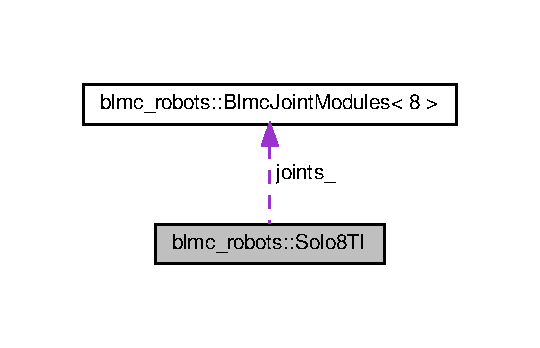
\includegraphics[width=259pt]{classblmc__robots_1_1Solo8TI__coll__graph}
\end{center}
\end{figure}
\subsection*{Public Member Functions}
\begin{DoxyCompactItemize}
\item 
\hyperlink{classblmc__robots_1_1Solo8TI_a5f969910cd1f1b263297e02691a0df5a}{Solo8\+TI} ()
\begin{DoxyCompactList}\small\item\em \hyperlink{classblmc__robots_1_1Solo8}{Solo8} is the constructor of the class. \end{DoxyCompactList}\item 
void \hyperlink{classblmc__robots_1_1Solo8TI_adf9f5ed10293942b1ce06d0d0116f61c}{initialize} ()
\begin{DoxyCompactList}\small\item\em initialize the robot by setting aligning the motors and calibrate the sensors to 0 \end{DoxyCompactList}\item 
\mbox{\Hypertarget{classblmc__robots_1_1Solo8TI_a5299053c499b95be35685aed60fc8d50}\label{classblmc__robots_1_1Solo8TI_a5299053c499b95be35685aed60fc8d50}} 
void \hyperlink{classblmc__robots_1_1Solo8TI_a5299053c499b95be35685aed60fc8d50}{send\+\_\+target\+\_\+joint\+\_\+torque} (const Eigen\+::\+Ref$<$ \hyperlink{common__header_8hpp_a98975ffbe0bca1296078e0350dfedd60}{Vector8d} $>$ target\+\_\+joint\+\_\+torque)
\begin{DoxyCompactList}\small\item\em send\+\_\+target\+\_\+torques sends the target currents to the motors \end{DoxyCompactList}\item 
void \hyperlink{classblmc__robots_1_1Solo8TI_a9241d0a805efd871a56d7cace099c208}{acquire\+\_\+sensors} ()
\begin{DoxyCompactList}\small\item\em acquire\+\_\+sensors acquire all available sensors, W\+A\+R\+N\+I\+NG !!!! this method has to be called prior to any getter to have up to date data. \end{DoxyCompactList}\item 
bool \hyperlink{classblmc__robots_1_1Solo8TI_a8ff4ec509f904ab3fab7268c75065c1f}{calibrate} (const \hyperlink{common__header_8hpp_a98975ffbe0bca1296078e0350dfedd60}{Vector8d} \&home\+\_\+offset\+\_\+rad)
\begin{DoxyCompactList}\small\item\em Calibrate the joints by moving to the next joint index position. \end{DoxyCompactList}\item 
const Eigen\+::\+Ref$<$ \hyperlink{common__header_8hpp_a98975ffbe0bca1296078e0350dfedd60}{Vector8d} $>$ \hyperlink{classblmc__robots_1_1Solo8TI_a21b4faac39d48f464cd29aea1c2eb9e2}{get\+\_\+motor\+\_\+inertias} ()
\begin{DoxyCompactList}\small\item\em Joint properties. \end{DoxyCompactList}\item 
const Eigen\+::\+Ref$<$ \hyperlink{common__header_8hpp_a98975ffbe0bca1296078e0350dfedd60}{Vector8d} $>$ \hyperlink{classblmc__robots_1_1Solo8TI_af421f0fa29744714c5e4a592501b972f}{get\+\_\+motor\+\_\+torque\+\_\+constants} ()
\begin{DoxyCompactList}\small\item\em get\+\_\+motor\+\_\+torque\+\_\+constants \end{DoxyCompactList}\item 
const Eigen\+::\+Ref$<$ \hyperlink{common__header_8hpp_a98975ffbe0bca1296078e0350dfedd60}{Vector8d} $>$ \hyperlink{classblmc__robots_1_1Solo8TI_a9f8c700d0646d5cc7f7e884b17aef1ab}{get\+\_\+joint\+\_\+gear\+\_\+ratios} ()
\begin{DoxyCompactList}\small\item\em get\+\_\+joint\+\_\+gear\+\_\+ratios \end{DoxyCompactList}\item 
const Eigen\+::\+Ref$<$ \hyperlink{common__header_8hpp_a98975ffbe0bca1296078e0350dfedd60}{Vector8d} $>$ \hyperlink{classblmc__robots_1_1Solo8TI_a6258a43a859e3cb589e7ed4ad7ca23cc}{get\+\_\+motor\+\_\+max\+\_\+current} ()
\begin{DoxyCompactList}\small\item\em get\+\_\+max\+\_\+torque \end{DoxyCompactList}\item 
const Eigen\+::\+Ref$<$ \hyperlink{common__header_8hpp_a98975ffbe0bca1296078e0350dfedd60}{Vector8d} $>$ \hyperlink{classblmc__robots_1_1Solo8TI_ac9165114408f88accbaa151b797ed1b6}{get\+\_\+joint\+\_\+positions} ()
\begin{DoxyCompactList}\small\item\em Sensor Data. \end{DoxyCompactList}\item 
const Eigen\+::\+Ref$<$ \hyperlink{common__header_8hpp_a98975ffbe0bca1296078e0350dfedd60}{Vector8d} $>$ \hyperlink{classblmc__robots_1_1Solo8TI_ae419d6776511856df3ff54e348774a97}{get\+\_\+joint\+\_\+velocities} ()
\begin{DoxyCompactList}\small\item\em get\+\_\+joint\+\_\+velocities \end{DoxyCompactList}\item 
const Eigen\+::\+Ref$<$ \hyperlink{common__header_8hpp_a98975ffbe0bca1296078e0350dfedd60}{Vector8d} $>$ \hyperlink{classblmc__robots_1_1Solo8TI_a79339925d2ad19cf8efff3af728a766f}{get\+\_\+joint\+\_\+torques} ()
\begin{DoxyCompactList}\small\item\em get\+\_\+joint\+\_\+torques \end{DoxyCompactList}\item 
const Eigen\+::\+Ref$<$ \hyperlink{common__header_8hpp_a98975ffbe0bca1296078e0350dfedd60}{Vector8d} $>$ \hyperlink{classblmc__robots_1_1Solo8TI_a3ed929d26586ef0aa35c4952e8c61f6d}{get\+\_\+joint\+\_\+target\+\_\+torques} ()
\begin{DoxyCompactList}\small\item\em get\+\_\+joint\+\_\+torques \end{DoxyCompactList}\item 
const Eigen\+::\+Ref$<$ \hyperlink{common__header_8hpp_a98975ffbe0bca1296078e0350dfedd60}{Vector8d} $>$ \hyperlink{classblmc__robots_1_1Solo8TI_a64832124d666033300a2d163db799f8a}{get\+\_\+joint\+\_\+encoder\+\_\+index} ()
\begin{DoxyCompactList}\small\item\em get\+\_\+joint\+\_\+encoder\+\_\+index \end{DoxyCompactList}\item 
const Eigen\+::\+Ref$<$ Eigen\+::\+Vector4d $>$ \hyperlink{classblmc__robots_1_1Solo8TI_aef169a78898e5ee8aaadc63942c3b7b6}{get\+\_\+contact\+\_\+sensors\+\_\+states} ()
\begin{DoxyCompactList}\small\item\em get\+\_\+contact\+\_\+sensors\+\_\+states \end{DoxyCompactList}\item 
const Eigen\+::\+Ref$<$ Eigen\+::\+Vector4d $>$ \hyperlink{classblmc__robots_1_1Solo8TI_ac02884b8402b774ce51c30be6fb4eda6}{get\+\_\+slider\+\_\+positions} ()
\begin{DoxyCompactList}\small\item\em get\+\_\+slider\+\_\+positions \end{DoxyCompactList}\item 
const std\+::array$<$ bool, 8 $>$ \& \hyperlink{classblmc__robots_1_1Solo8TI_acd7e33f11be0d4e63030d1ec4815eba5}{get\+\_\+motor\+\_\+enabled} ()
\begin{DoxyCompactList}\small\item\em Hardware Status. \end{DoxyCompactList}\item 
const std\+::array$<$ bool, 8 $>$ \& \hyperlink{classblmc__robots_1_1Solo8TI_ae0572a7d9b2ec2b4c63188d0957c5b6f}{get\+\_\+motor\+\_\+ready} ()
\begin{DoxyCompactList}\small\item\em get\+\_\+motor\+\_\+ready \end{DoxyCompactList}\item 
const std\+::array$<$ bool, 4 $>$ \& \hyperlink{classblmc__robots_1_1Solo8TI_a1c99bf64212b2b5c84f7ccfbdea5b935}{get\+\_\+motor\+\_\+board\+\_\+enabled} ()
\begin{DoxyCompactList}\small\item\em get\+\_\+motor\+\_\+board\+\_\+enabled \end{DoxyCompactList}\item 
const std\+::array$<$ int, 4 $>$ \& \hyperlink{classblmc__robots_1_1Solo8TI_aa7d82d290e330c86af2f21d16098c460}{get\+\_\+motor\+\_\+board\+\_\+errors} ()
\begin{DoxyCompactList}\small\item\em get\+\_\+motor\+\_\+board\+\_\+errors \end{DoxyCompactList}\end{DoxyCompactItemize}
\subsection*{Private Attributes}
\begin{DoxyCompactItemize}
\item 
\hyperlink{common__header_8hpp_a98975ffbe0bca1296078e0350dfedd60}{Vector8d} \hyperlink{classblmc__robots_1_1Solo8TI_a59f11040a17d232823756c26c6b68145}{motor\+\_\+inertias\+\_\+}
\begin{DoxyCompactList}\small\item\em Motor data. \end{DoxyCompactList}\item 
\hyperlink{common__header_8hpp_a98975ffbe0bca1296078e0350dfedd60}{Vector8d} \hyperlink{classblmc__robots_1_1Solo8TI_ac2b9093468149839f7d6a6be43d108e7}{motor\+\_\+torque\+\_\+constants\+\_\+}
\begin{DoxyCompactList}\small\item\em D\+CM motor torque constants. \end{DoxyCompactList}\item 
\hyperlink{common__header_8hpp_a98975ffbe0bca1296078e0350dfedd60}{Vector8d} \hyperlink{classblmc__robots_1_1Solo8TI_a670ec9c986127612259d66e4f33d20b3}{joint\+\_\+gear\+\_\+ratios\+\_\+}
\begin{DoxyCompactList}\small\item\em joint gear ratios (9). \end{DoxyCompactList}\item 
\hyperlink{common__header_8hpp_a98975ffbe0bca1296078e0350dfedd60}{Vector8d} \hyperlink{classblmc__robots_1_1Solo8TI_afc3ba4524871faadbc1150f40e013f95}{motor\+\_\+max\+\_\+current\+\_\+}
\begin{DoxyCompactList}\small\item\em Max appliable current before the robot shutdown. \end{DoxyCompactList}\item 
\hyperlink{common__header_8hpp_a98975ffbe0bca1296078e0350dfedd60}{Vector8d} \hyperlink{classblmc__robots_1_1Solo8TI_a9dfb11213122b0a882dd54720ec719c3}{joint\+\_\+zero\+\_\+positions\+\_\+}
\begin{DoxyCompactList}\small\item\em Offset to the theoretical \char`\"{}0\char`\"{} pose. \end{DoxyCompactList}\item 
\mbox{\Hypertarget{classblmc__robots_1_1Solo8TI_a9eca8246a28a6f2f2d1deff52228e69f}\label{classblmc__robots_1_1Solo8TI_a9eca8246a28a6f2f2d1deff52228e69f}} 
Eigen\+::\+Array$<$ double, 8, 1 $>$ \hyperlink{classblmc__robots_1_1Solo8TI_a9eca8246a28a6f2f2d1deff52228e69f}{max\+\_\+joint\+\_\+torques\+\_\+}
\begin{DoxyCompactList}\small\item\em Max joint torques (Nm) \end{DoxyCompactList}\item 
std\+::array$<$ bool, 8 $>$ \hyperlink{classblmc__robots_1_1Solo8TI_a3dbd4bd26b5a4273e94ced22d43a9890}{motor\+\_\+enabled\+\_\+}
\begin{DoxyCompactList}\small\item\em Hardware status. \end{DoxyCompactList}\item 
\mbox{\Hypertarget{classblmc__robots_1_1Solo8TI_a604140f307df2c420c29990948fdbd38}\label{classblmc__robots_1_1Solo8TI_a604140f307df2c420c29990948fdbd38}} 
std\+::array$<$ bool, 8 $>$ \hyperlink{classblmc__robots_1_1Solo8TI_a604140f307df2c420c29990948fdbd38}{motor\+\_\+ready\+\_\+}
\begin{DoxyCompactList}\small\item\em This gives the status (enabled/disabled) of each motors using the joint ordering convention. \end{DoxyCompactList}\item 
\mbox{\Hypertarget{classblmc__robots_1_1Solo8TI_a9471bb2684e782adfc1a8db58ba9c18e}\label{classblmc__robots_1_1Solo8TI_a9471bb2684e782adfc1a8db58ba9c18e}} 
std\+::array$<$ bool, 4 $>$ \hyperlink{classblmc__robots_1_1Solo8TI_a9471bb2684e782adfc1a8db58ba9c18e}{motor\+\_\+board\+\_\+enabled\+\_\+}
\begin{DoxyCompactList}\small\item\em This gives the status (enabled/disabled of the onboard control cards). \end{DoxyCompactList}\item 
\mbox{\Hypertarget{classblmc__robots_1_1Solo8TI_a3621a7c3174f44ba3051577588d55c88}\label{classblmc__robots_1_1Solo8TI_a3621a7c3174f44ba3051577588d55c88}} 
std\+::array$<$ int, 4 $>$ \hyperlink{classblmc__robots_1_1Solo8TI_a3621a7c3174f44ba3051577588d55c88}{motor\+\_\+board\+\_\+errors\+\_\+}
\begin{DoxyCompactList}\small\item\em This gives the status (enabled/disabled of the onboard control cards). \end{DoxyCompactList}\item 
\hyperlink{common__header_8hpp_a98975ffbe0bca1296078e0350dfedd60}{Vector8d} \hyperlink{classblmc__robots_1_1Solo8TI_a6ca7d08522f038dc47d6a97f937c6f75}{joint\+\_\+positions\+\_\+}
\begin{DoxyCompactList}\small\item\em Joint data. \end{DoxyCompactList}\item 
\mbox{\Hypertarget{classblmc__robots_1_1Solo8TI_a12037a7a9b29e70df344fcf59b181f01}\label{classblmc__robots_1_1Solo8TI_a12037a7a9b29e70df344fcf59b181f01}} 
\hyperlink{common__header_8hpp_a98975ffbe0bca1296078e0350dfedd60}{Vector8d} \hyperlink{classblmc__robots_1_1Solo8TI_a12037a7a9b29e70df344fcf59b181f01}{joint\+\_\+velocities\+\_\+}
\begin{DoxyCompactList}\small\item\em joint\+\_\+velocities\+\_\+ \end{DoxyCompactList}\item 
\mbox{\Hypertarget{classblmc__robots_1_1Solo8TI_a622faae774063f90854a8968535ec38e}\label{classblmc__robots_1_1Solo8TI_a622faae774063f90854a8968535ec38e}} 
\hyperlink{common__header_8hpp_a98975ffbe0bca1296078e0350dfedd60}{Vector8d} \hyperlink{classblmc__robots_1_1Solo8TI_a622faae774063f90854a8968535ec38e}{joint\+\_\+torques\+\_\+}
\begin{DoxyCompactList}\small\item\em joint\+\_\+torques\+\_\+ \end{DoxyCompactList}\item 
\mbox{\Hypertarget{classblmc__robots_1_1Solo8TI_ad10b73e34b2fc2f46592250c631f3f8c}\label{classblmc__robots_1_1Solo8TI_ad10b73e34b2fc2f46592250c631f3f8c}} 
\hyperlink{common__header_8hpp_a98975ffbe0bca1296078e0350dfedd60}{Vector8d} \hyperlink{classblmc__robots_1_1Solo8TI_ad10b73e34b2fc2f46592250c631f3f8c}{joint\+\_\+target\+\_\+torques\+\_\+}
\begin{DoxyCompactList}\small\item\em joint\+\_\+target\+\_\+torques\+\_\+ \end{DoxyCompactList}\item 
\mbox{\Hypertarget{classblmc__robots_1_1Solo8TI_ae20202e31405b58cdc14bd6e4935c68c}\label{classblmc__robots_1_1Solo8TI_ae20202e31405b58cdc14bd6e4935c68c}} 
\hyperlink{common__header_8hpp_a98975ffbe0bca1296078e0350dfedd60}{Vector8d} \hyperlink{classblmc__robots_1_1Solo8TI_ae20202e31405b58cdc14bd6e4935c68c}{joint\+\_\+encoder\+\_\+index\+\_\+}
\begin{DoxyCompactList}\small\item\em joint\+\_\+encoder\+\_\+index\+\_\+ \end{DoxyCompactList}\item 
Eigen\+::\+Vector4d \hyperlink{classblmc__robots_1_1Solo8TI_ac81e772bd951a26989c1b9108eccecec}{slider\+\_\+positions\+\_\+}
\begin{DoxyCompactList}\small\item\em Additional data. \end{DoxyCompactList}\item 
\mbox{\Hypertarget{classblmc__robots_1_1Solo8TI_a0890fcba8970fa8d9a3442ff8f4c9015}\label{classblmc__robots_1_1Solo8TI_a0890fcba8970fa8d9a3442ff8f4c9015}} 
Eigen\+::\+Vector4d \hyperlink{classblmc__robots_1_1Solo8TI_a0890fcba8970fa8d9a3442ff8f4c9015}{contact\+\_\+sensors\+\_\+states\+\_\+}
\begin{DoxyCompactList}\small\item\em contact\+\_\+sensors\+\_\+ is contact sensors at each feet of teh quadruped. \end{DoxyCompactList}\item 
std\+::array$<$ int, 8 $>$ \hyperlink{classblmc__robots_1_1Solo8TI_a1287fd44d615eec9d3333f186adb18ec}{motor\+\_\+to\+\_\+card\+\_\+index\+\_\+}
\begin{DoxyCompactList}\small\item\em Drivers communication objects. \end{DoxyCompactList}\item 
\mbox{\Hypertarget{classblmc__robots_1_1Solo8TI_ae85c5b55fc3ac22ab6d28533f544fff5}\label{classblmc__robots_1_1Solo8TI_ae85c5b55fc3ac22ab6d28533f544fff5}} 
std\+::array$<$ int, 8 $>$ \hyperlink{classblmc__robots_1_1Solo8TI_ae85c5b55fc3ac22ab6d28533f544fff5}{motor\+\_\+to\+\_\+card\+\_\+port\+\_\+index\+\_\+}
\begin{DoxyCompactList}\small\item\em This map for every motor the card port. \end{DoxyCompactList}\item 
\mbox{\Hypertarget{classblmc__robots_1_1Solo8TI_a1dc6570d3d386a8f955ca83566dc2f9b}\label{classblmc__robots_1_1Solo8TI_a1dc6570d3d386a8f955ca83566dc2f9b}} 
std\+::array$<$ \hyperlink{common__header_8hpp_a793c8789a7598e8aaf766939da7262af}{Can\+Bus\+\_\+ptr}, 4 $>$ \hyperlink{classblmc__robots_1_1Solo8TI_a1dc6570d3d386a8f955ca83566dc2f9b}{can\+\_\+buses\+\_\+}
\begin{DoxyCompactList}\small\item\em can\+\_\+buses\+\_\+ are the 4 can buses on the robot. \end{DoxyCompactList}\item 
\mbox{\Hypertarget{classblmc__robots_1_1Solo8TI_aa436a497b597b05b0733430ea5c2f251}\label{classblmc__robots_1_1Solo8TI_aa436a497b597b05b0733430ea5c2f251}} 
std\+::array$<$ \hyperlink{common__header_8hpp_aab1c6ddb1273247a1b45d5e8b417c216}{Can\+Bus\+Motor\+Board\+\_\+ptr}, 4 $>$ \hyperlink{classblmc__robots_1_1Solo8TI_aa436a497b597b05b0733430ea5c2f251}{can\+\_\+motor\+\_\+boards\+\_\+}
\begin{DoxyCompactList}\small\item\em can\+\_\+motor\+\_\+boards\+\_\+ are the 4 can motor board. \end{DoxyCompactList}\item 
\mbox{\Hypertarget{classblmc__robots_1_1Solo8TI_a369f7f53f6bb02e325616ebcf9a4fd88}\label{classblmc__robots_1_1Solo8TI_a369f7f53f6bb02e325616ebcf9a4fd88}} 
std\+::array$<$ \hyperlink{common__header_8hpp_ae1a0f9992bc8fbbc1943d887f517c180}{Motor\+Interface\+\_\+ptr}, 8 $>$ \hyperlink{classblmc__robots_1_1Solo8TI_a369f7f53f6bb02e325616ebcf9a4fd88}{motors\+\_\+}
\begin{DoxyCompactList}\small\item\em motors\+\_\+ are the objects allowing us to send motor commands and receive data. \end{DoxyCompactList}\item 
\mbox{\Hypertarget{classblmc__robots_1_1Solo8TI_ab1b54a7f74cfda8bd537d0adfc21166c}\label{classblmc__robots_1_1Solo8TI_ab1b54a7f74cfda8bd537d0adfc21166c}} 
\hyperlink{classblmc__robots_1_1BlmcJointModules}{Blmc\+Joint\+Modules}$<$ 8 $>$ \hyperlink{classblmc__robots_1_1Solo8TI_ab1b54a7f74cfda8bd537d0adfc21166c}{joints\+\_\+}
\begin{DoxyCompactList}\small\item\em This is the collection of joints that compose the robot. \end{DoxyCompactList}\item 
\mbox{\Hypertarget{classblmc__robots_1_1Solo8TI_ab706eca1708afb98625a50c8347fd3d3}\label{classblmc__robots_1_1Solo8TI_ab706eca1708afb98625a50c8347fd3d3}} 
std\+::array$<$ bool, 8 $>$ \hyperlink{classblmc__robots_1_1Solo8TI_ab706eca1708afb98625a50c8347fd3d3}{reverse\+\_\+polarities\+\_\+}
\begin{DoxyCompactList}\small\item\em Address the rotation direction of the motor. \end{DoxyCompactList}\item 
\mbox{\Hypertarget{classblmc__robots_1_1Solo8TI_ae4f93fdbb8c382e5b317e471f9c7c429}\label{classblmc__robots_1_1Solo8TI_ae4f93fdbb8c382e5b317e471f9c7c429}} 
std\+::array$<$ \hyperlink{common__header_8hpp_a4cb9a95e8b2c0bf237ce29f5252c7b73}{Slider\+\_\+ptr}, 4 $>$ \hyperlink{classblmc__robots_1_1Solo8TI_ae4f93fdbb8c382e5b317e471f9c7c429}{sliders\+\_\+}
\begin{DoxyCompactList}\small\item\em sliders\+\_\+ these are analogue input from linear potentiometers. \end{DoxyCompactList}\item 
std\+::array$<$ \hyperlink{common__header_8hpp_ac78fe5c68e56a3b884117109959e4d58}{Contact\+Sensor\+\_\+ptr}, 4 $>$ \hyperlink{classblmc__robots_1_1Solo8TI_afc6e87d1cec24fd373345e41df874baf}{contact\+\_\+sensors\+\_\+}
\begin{DoxyCompactList}\small\item\em contact\+\_\+sensors\+\_\+ is the contact sensors at each foot tips. \end{DoxyCompactList}\end{DoxyCompactItemize}
\subsection*{Static Private Attributes}
\begin{DoxyCompactItemize}
\item 
static const double \hyperlink{classblmc__robots_1_1Solo8TI_ab2e5018719efa9ea068a4dc870fbb82e}{max\+\_\+joint\+\_\+torque\+\_\+security\+\_\+margin\+\_\+} = 0.\+99
\begin{DoxyCompactList}\small\item\em Security margin on the saturation of the control. \end{DoxyCompactList}\end{DoxyCompactItemize}


\subsection{Constructor \& Destructor Documentation}
\mbox{\Hypertarget{classblmc__robots_1_1Solo8TI_a5f969910cd1f1b263297e02691a0df5a}\label{classblmc__robots_1_1Solo8TI_a5f969910cd1f1b263297e02691a0df5a}} 
\index{blmc\+\_\+robots\+::\+Solo8\+TI@{blmc\+\_\+robots\+::\+Solo8\+TI}!Solo8\+TI@{Solo8\+TI}}
\index{Solo8\+TI@{Solo8\+TI}!blmc\+\_\+robots\+::\+Solo8\+TI@{blmc\+\_\+robots\+::\+Solo8\+TI}}
\subsubsection{\texorpdfstring{Solo8\+T\+I()}{Solo8TI()}}
{\footnotesize\ttfamily blmc\+\_\+robots\+::\+Solo8\+T\+I\+::\+Solo8\+TI (\begin{DoxyParamCaption}{ }\end{DoxyParamCaption})}



\hyperlink{classblmc__robots_1_1Solo8}{Solo8} is the constructor of the class. 

Hardware properties

Hardware status

Joint data

Additional data

Setup some known data

\subsection{Member Function Documentation}
\mbox{\Hypertarget{classblmc__robots_1_1Solo8TI_a9241d0a805efd871a56d7cace099c208}\label{classblmc__robots_1_1Solo8TI_a9241d0a805efd871a56d7cace099c208}} 
\index{blmc\+\_\+robots\+::\+Solo8\+TI@{blmc\+\_\+robots\+::\+Solo8\+TI}!acquire\+\_\+sensors@{acquire\+\_\+sensors}}
\index{acquire\+\_\+sensors@{acquire\+\_\+sensors}!blmc\+\_\+robots\+::\+Solo8\+TI@{blmc\+\_\+robots\+::\+Solo8\+TI}}
\subsubsection{\texorpdfstring{acquire\+\_\+sensors()}{acquire\_sensors()}}
{\footnotesize\ttfamily void blmc\+\_\+robots\+::\+Solo8\+T\+I\+::acquire\+\_\+sensors (\begin{DoxyParamCaption}{ }\end{DoxyParamCaption})}



acquire\+\_\+sensors acquire all available sensors, W\+A\+R\+N\+I\+NG !!!! this method has to be called prior to any getter to have up to date data. 

Joint data

Additional data

The different status.\mbox{\Hypertarget{classblmc__robots_1_1Solo8TI_a8ff4ec509f904ab3fab7268c75065c1f}\label{classblmc__robots_1_1Solo8TI_a8ff4ec509f904ab3fab7268c75065c1f}} 
\index{blmc\+\_\+robots\+::\+Solo8\+TI@{blmc\+\_\+robots\+::\+Solo8\+TI}!calibrate@{calibrate}}
\index{calibrate@{calibrate}!blmc\+\_\+robots\+::\+Solo8\+TI@{blmc\+\_\+robots\+::\+Solo8\+TI}}
\subsubsection{\texorpdfstring{calibrate()}{calibrate()}}
{\footnotesize\ttfamily bool blmc\+\_\+robots\+::\+Solo8\+T\+I\+::calibrate (\begin{DoxyParamCaption}\item[{const \hyperlink{common__header_8hpp_a98975ffbe0bca1296078e0350dfedd60}{Vector8d} \&}]{home\+\_\+offset\+\_\+rad }\end{DoxyParamCaption})}



Calibrate the joints by moving to the next joint index position. 


\begin{DoxyParams}{Parameters}
{\em home\+\_\+offset\+\_\+rad} & This is the angle between the index and the zero pose. \\
\hline
\end{DoxyParams}
\begin{DoxyReturn}{Returns}
true 

false 
\end{DoxyReturn}
\mbox{\Hypertarget{classblmc__robots_1_1Solo8TI_aef169a78898e5ee8aaadc63942c3b7b6}\label{classblmc__robots_1_1Solo8TI_aef169a78898e5ee8aaadc63942c3b7b6}} 
\index{blmc\+\_\+robots\+::\+Solo8\+TI@{blmc\+\_\+robots\+::\+Solo8\+TI}!get\+\_\+contact\+\_\+sensors\+\_\+states@{get\+\_\+contact\+\_\+sensors\+\_\+states}}
\index{get\+\_\+contact\+\_\+sensors\+\_\+states@{get\+\_\+contact\+\_\+sensors\+\_\+states}!blmc\+\_\+robots\+::\+Solo8\+TI@{blmc\+\_\+robots\+::\+Solo8\+TI}}
\subsubsection{\texorpdfstring{get\+\_\+contact\+\_\+sensors\+\_\+states()}{get\_contact\_sensors\_states()}}
{\footnotesize\ttfamily const Eigen\+::\+Ref$<$Eigen\+::\+Vector4d$>$ blmc\+\_\+robots\+::\+Solo8\+T\+I\+::get\+\_\+contact\+\_\+sensors\+\_\+states (\begin{DoxyParamCaption}{ }\end{DoxyParamCaption})\hspace{0.3cm}{\ttfamily [inline]}}



get\+\_\+contact\+\_\+sensors\+\_\+states 

\begin{DoxyReturn}{Returns}
the state of the contacts states W\+A\+R\+N\+I\+NG !!!! The method $<$acquire\+\_\+sensors$>$\char`\"{}()\char`\"{} has to be called prior to any getter to have up to date data. 
\end{DoxyReturn}
\mbox{\Hypertarget{classblmc__robots_1_1Solo8TI_a64832124d666033300a2d163db799f8a}\label{classblmc__robots_1_1Solo8TI_a64832124d666033300a2d163db799f8a}} 
\index{blmc\+\_\+robots\+::\+Solo8\+TI@{blmc\+\_\+robots\+::\+Solo8\+TI}!get\+\_\+joint\+\_\+encoder\+\_\+index@{get\+\_\+joint\+\_\+encoder\+\_\+index}}
\index{get\+\_\+joint\+\_\+encoder\+\_\+index@{get\+\_\+joint\+\_\+encoder\+\_\+index}!blmc\+\_\+robots\+::\+Solo8\+TI@{blmc\+\_\+robots\+::\+Solo8\+TI}}
\subsubsection{\texorpdfstring{get\+\_\+joint\+\_\+encoder\+\_\+index()}{get\_joint\_encoder\_index()}}
{\footnotesize\ttfamily const Eigen\+::\+Ref$<$\hyperlink{common__header_8hpp_a98975ffbe0bca1296078e0350dfedd60}{Vector8d}$>$ blmc\+\_\+robots\+::\+Solo8\+T\+I\+::get\+\_\+joint\+\_\+encoder\+\_\+index (\begin{DoxyParamCaption}{ }\end{DoxyParamCaption})\hspace{0.3cm}{\ttfamily [inline]}}



get\+\_\+joint\+\_\+encoder\+\_\+index 

\begin{DoxyReturn}{Returns}
the position of the index of the encoders a the motor level W\+A\+R\+N\+I\+NG !!!! The method $<$acquire\+\_\+sensors$>$\char`\"{}()\char`\"{} has to be called prior to any getter to have up to date data. 
\end{DoxyReturn}
\mbox{\Hypertarget{classblmc__robots_1_1Solo8TI_a9f8c700d0646d5cc7f7e884b17aef1ab}\label{classblmc__robots_1_1Solo8TI_a9f8c700d0646d5cc7f7e884b17aef1ab}} 
\index{blmc\+\_\+robots\+::\+Solo8\+TI@{blmc\+\_\+robots\+::\+Solo8\+TI}!get\+\_\+joint\+\_\+gear\+\_\+ratios@{get\+\_\+joint\+\_\+gear\+\_\+ratios}}
\index{get\+\_\+joint\+\_\+gear\+\_\+ratios@{get\+\_\+joint\+\_\+gear\+\_\+ratios}!blmc\+\_\+robots\+::\+Solo8\+TI@{blmc\+\_\+robots\+::\+Solo8\+TI}}
\subsubsection{\texorpdfstring{get\+\_\+joint\+\_\+gear\+\_\+ratios()}{get\_joint\_gear\_ratios()}}
{\footnotesize\ttfamily const Eigen\+::\+Ref$<$\hyperlink{common__header_8hpp_a98975ffbe0bca1296078e0350dfedd60}{Vector8d}$>$ blmc\+\_\+robots\+::\+Solo8\+T\+I\+::get\+\_\+joint\+\_\+gear\+\_\+ratios (\begin{DoxyParamCaption}{ }\end{DoxyParamCaption})\hspace{0.3cm}{\ttfamily [inline]}}



get\+\_\+joint\+\_\+gear\+\_\+ratios 

\begin{DoxyReturn}{Returns}
the joint gear ratios 
\end{DoxyReturn}
\mbox{\Hypertarget{classblmc__robots_1_1Solo8TI_ac9165114408f88accbaa151b797ed1b6}\label{classblmc__robots_1_1Solo8TI_ac9165114408f88accbaa151b797ed1b6}} 
\index{blmc\+\_\+robots\+::\+Solo8\+TI@{blmc\+\_\+robots\+::\+Solo8\+TI}!get\+\_\+joint\+\_\+positions@{get\+\_\+joint\+\_\+positions}}
\index{get\+\_\+joint\+\_\+positions@{get\+\_\+joint\+\_\+positions}!blmc\+\_\+robots\+::\+Solo8\+TI@{blmc\+\_\+robots\+::\+Solo8\+TI}}
\subsubsection{\texorpdfstring{get\+\_\+joint\+\_\+positions()}{get\_joint\_positions()}}
{\footnotesize\ttfamily const Eigen\+::\+Ref$<$\hyperlink{common__header_8hpp_a98975ffbe0bca1296078e0350dfedd60}{Vector8d}$>$ blmc\+\_\+robots\+::\+Solo8\+T\+I\+::get\+\_\+joint\+\_\+positions (\begin{DoxyParamCaption}{ }\end{DoxyParamCaption})\hspace{0.3cm}{\ttfamily [inline]}}



Sensor Data. 

get\+\_\+joint\+\_\+positions \begin{DoxyReturn}{Returns}
the joint angle of each module W\+A\+R\+N\+I\+NG !!!! The method $<$acquire\+\_\+sensors$>$\char`\"{}()\char`\"{} has to be called prior to any getter to have up to date data. 
\end{DoxyReturn}
\mbox{\Hypertarget{classblmc__robots_1_1Solo8TI_a3ed929d26586ef0aa35c4952e8c61f6d}\label{classblmc__robots_1_1Solo8TI_a3ed929d26586ef0aa35c4952e8c61f6d}} 
\index{blmc\+\_\+robots\+::\+Solo8\+TI@{blmc\+\_\+robots\+::\+Solo8\+TI}!get\+\_\+joint\+\_\+target\+\_\+torques@{get\+\_\+joint\+\_\+target\+\_\+torques}}
\index{get\+\_\+joint\+\_\+target\+\_\+torques@{get\+\_\+joint\+\_\+target\+\_\+torques}!blmc\+\_\+robots\+::\+Solo8\+TI@{blmc\+\_\+robots\+::\+Solo8\+TI}}
\subsubsection{\texorpdfstring{get\+\_\+joint\+\_\+target\+\_\+torques()}{get\_joint\_target\_torques()}}
{\footnotesize\ttfamily const Eigen\+::\+Ref$<$\hyperlink{common__header_8hpp_a98975ffbe0bca1296078e0350dfedd60}{Vector8d}$>$ blmc\+\_\+robots\+::\+Solo8\+T\+I\+::get\+\_\+joint\+\_\+target\+\_\+torques (\begin{DoxyParamCaption}{ }\end{DoxyParamCaption})\hspace{0.3cm}{\ttfamily [inline]}}



get\+\_\+joint\+\_\+torques 

\begin{DoxyReturn}{Returns}
the target joint torques W\+A\+R\+N\+I\+NG !!!! The method $<$acquire\+\_\+sensors$>$\char`\"{}()\char`\"{} has to be called prior to any getter to have up to date data. 
\end{DoxyReturn}
\mbox{\Hypertarget{classblmc__robots_1_1Solo8TI_a79339925d2ad19cf8efff3af728a766f}\label{classblmc__robots_1_1Solo8TI_a79339925d2ad19cf8efff3af728a766f}} 
\index{blmc\+\_\+robots\+::\+Solo8\+TI@{blmc\+\_\+robots\+::\+Solo8\+TI}!get\+\_\+joint\+\_\+torques@{get\+\_\+joint\+\_\+torques}}
\index{get\+\_\+joint\+\_\+torques@{get\+\_\+joint\+\_\+torques}!blmc\+\_\+robots\+::\+Solo8\+TI@{blmc\+\_\+robots\+::\+Solo8\+TI}}
\subsubsection{\texorpdfstring{get\+\_\+joint\+\_\+torques()}{get\_joint\_torques()}}
{\footnotesize\ttfamily const Eigen\+::\+Ref$<$\hyperlink{common__header_8hpp_a98975ffbe0bca1296078e0350dfedd60}{Vector8d}$>$ blmc\+\_\+robots\+::\+Solo8\+T\+I\+::get\+\_\+joint\+\_\+torques (\begin{DoxyParamCaption}{ }\end{DoxyParamCaption})\hspace{0.3cm}{\ttfamily [inline]}}



get\+\_\+joint\+\_\+torques 

\begin{DoxyReturn}{Returns}
the joint torques W\+A\+R\+N\+I\+NG !!!! The method $<$acquire\+\_\+sensors$>$\char`\"{}()\char`\"{} has to be called prior to any getter to have up to date data. 
\end{DoxyReturn}
\mbox{\Hypertarget{classblmc__robots_1_1Solo8TI_ae419d6776511856df3ff54e348774a97}\label{classblmc__robots_1_1Solo8TI_ae419d6776511856df3ff54e348774a97}} 
\index{blmc\+\_\+robots\+::\+Solo8\+TI@{blmc\+\_\+robots\+::\+Solo8\+TI}!get\+\_\+joint\+\_\+velocities@{get\+\_\+joint\+\_\+velocities}}
\index{get\+\_\+joint\+\_\+velocities@{get\+\_\+joint\+\_\+velocities}!blmc\+\_\+robots\+::\+Solo8\+TI@{blmc\+\_\+robots\+::\+Solo8\+TI}}
\subsubsection{\texorpdfstring{get\+\_\+joint\+\_\+velocities()}{get\_joint\_velocities()}}
{\footnotesize\ttfamily const Eigen\+::\+Ref$<$\hyperlink{common__header_8hpp_a98975ffbe0bca1296078e0350dfedd60}{Vector8d}$>$ blmc\+\_\+robots\+::\+Solo8\+T\+I\+::get\+\_\+joint\+\_\+velocities (\begin{DoxyParamCaption}{ }\end{DoxyParamCaption})\hspace{0.3cm}{\ttfamily [inline]}}



get\+\_\+joint\+\_\+velocities 

\begin{DoxyReturn}{Returns}
the joint velocities W\+A\+R\+N\+I\+NG !!!! The method $<$acquire\+\_\+sensors$>$\char`\"{}()\char`\"{} has to be called prior to any getter to have up to date data. 
\end{DoxyReturn}
\mbox{\Hypertarget{classblmc__robots_1_1Solo8TI_a1c99bf64212b2b5c84f7ccfbdea5b935}\label{classblmc__robots_1_1Solo8TI_a1c99bf64212b2b5c84f7ccfbdea5b935}} 
\index{blmc\+\_\+robots\+::\+Solo8\+TI@{blmc\+\_\+robots\+::\+Solo8\+TI}!get\+\_\+motor\+\_\+board\+\_\+enabled@{get\+\_\+motor\+\_\+board\+\_\+enabled}}
\index{get\+\_\+motor\+\_\+board\+\_\+enabled@{get\+\_\+motor\+\_\+board\+\_\+enabled}!blmc\+\_\+robots\+::\+Solo8\+TI@{blmc\+\_\+robots\+::\+Solo8\+TI}}
\subsubsection{\texorpdfstring{get\+\_\+motor\+\_\+board\+\_\+enabled()}{get\_motor\_board\_enabled()}}
{\footnotesize\ttfamily const std\+::array$<$bool, 4$>$\& blmc\+\_\+robots\+::\+Solo8\+T\+I\+::get\+\_\+motor\+\_\+board\+\_\+enabled (\begin{DoxyParamCaption}{ }\end{DoxyParamCaption})\hspace{0.3cm}{\ttfamily [inline]}}



get\+\_\+motor\+\_\+board\+\_\+enabled 

\begin{DoxyReturn}{Returns}
This gives the status (enabled/disabled of the onboard control cards). 
\end{DoxyReturn}
\mbox{\Hypertarget{classblmc__robots_1_1Solo8TI_aa7d82d290e330c86af2f21d16098c460}\label{classblmc__robots_1_1Solo8TI_aa7d82d290e330c86af2f21d16098c460}} 
\index{blmc\+\_\+robots\+::\+Solo8\+TI@{blmc\+\_\+robots\+::\+Solo8\+TI}!get\+\_\+motor\+\_\+board\+\_\+errors@{get\+\_\+motor\+\_\+board\+\_\+errors}}
\index{get\+\_\+motor\+\_\+board\+\_\+errors@{get\+\_\+motor\+\_\+board\+\_\+errors}!blmc\+\_\+robots\+::\+Solo8\+TI@{blmc\+\_\+robots\+::\+Solo8\+TI}}
\subsubsection{\texorpdfstring{get\+\_\+motor\+\_\+board\+\_\+errors()}{get\_motor\_board\_errors()}}
{\footnotesize\ttfamily const std\+::array$<$int, 4$>$\& blmc\+\_\+robots\+::\+Solo8\+T\+I\+::get\+\_\+motor\+\_\+board\+\_\+errors (\begin{DoxyParamCaption}{ }\end{DoxyParamCaption})\hspace{0.3cm}{\ttfamily [inline]}}



get\+\_\+motor\+\_\+board\+\_\+errors 

\begin{DoxyReturn}{Returns}
This gives the status (enabled/disabled of the onboard control cards). 
\end{DoxyReturn}
\mbox{\Hypertarget{classblmc__robots_1_1Solo8TI_acd7e33f11be0d4e63030d1ec4815eba5}\label{classblmc__robots_1_1Solo8TI_acd7e33f11be0d4e63030d1ec4815eba5}} 
\index{blmc\+\_\+robots\+::\+Solo8\+TI@{blmc\+\_\+robots\+::\+Solo8\+TI}!get\+\_\+motor\+\_\+enabled@{get\+\_\+motor\+\_\+enabled}}
\index{get\+\_\+motor\+\_\+enabled@{get\+\_\+motor\+\_\+enabled}!blmc\+\_\+robots\+::\+Solo8\+TI@{blmc\+\_\+robots\+::\+Solo8\+TI}}
\subsubsection{\texorpdfstring{get\+\_\+motor\+\_\+enabled()}{get\_motor\_enabled()}}
{\footnotesize\ttfamily const std\+::array$<$bool, 8$>$\& blmc\+\_\+robots\+::\+Solo8\+T\+I\+::get\+\_\+motor\+\_\+enabled (\begin{DoxyParamCaption}{ }\end{DoxyParamCaption})\hspace{0.3cm}{\ttfamily [inline]}}



Hardware Status. 

get\+\_\+motor\+\_\+enabled \begin{DoxyReturn}{Returns}
This gives the status (enabled/disabled) of each motors using the joint ordering convention. 
\end{DoxyReturn}
\mbox{\Hypertarget{classblmc__robots_1_1Solo8TI_a21b4faac39d48f464cd29aea1c2eb9e2}\label{classblmc__robots_1_1Solo8TI_a21b4faac39d48f464cd29aea1c2eb9e2}} 
\index{blmc\+\_\+robots\+::\+Solo8\+TI@{blmc\+\_\+robots\+::\+Solo8\+TI}!get\+\_\+motor\+\_\+inertias@{get\+\_\+motor\+\_\+inertias}}
\index{get\+\_\+motor\+\_\+inertias@{get\+\_\+motor\+\_\+inertias}!blmc\+\_\+robots\+::\+Solo8\+TI@{blmc\+\_\+robots\+::\+Solo8\+TI}}
\subsubsection{\texorpdfstring{get\+\_\+motor\+\_\+inertias()}{get\_motor\_inertias()}}
{\footnotesize\ttfamily const Eigen\+::\+Ref$<$\hyperlink{common__header_8hpp_a98975ffbe0bca1296078e0350dfedd60}{Vector8d}$>$ blmc\+\_\+robots\+::\+Solo8\+T\+I\+::get\+\_\+motor\+\_\+inertias (\begin{DoxyParamCaption}{ }\end{DoxyParamCaption})\hspace{0.3cm}{\ttfamily [inline]}}



Joint properties. 

get\+\_\+motor\+\_\+inertias \begin{DoxyReturn}{Returns}
the motor inertias 
\end{DoxyReturn}
\mbox{\Hypertarget{classblmc__robots_1_1Solo8TI_a6258a43a859e3cb589e7ed4ad7ca23cc}\label{classblmc__robots_1_1Solo8TI_a6258a43a859e3cb589e7ed4ad7ca23cc}} 
\index{blmc\+\_\+robots\+::\+Solo8\+TI@{blmc\+\_\+robots\+::\+Solo8\+TI}!get\+\_\+motor\+\_\+max\+\_\+current@{get\+\_\+motor\+\_\+max\+\_\+current}}
\index{get\+\_\+motor\+\_\+max\+\_\+current@{get\+\_\+motor\+\_\+max\+\_\+current}!blmc\+\_\+robots\+::\+Solo8\+TI@{blmc\+\_\+robots\+::\+Solo8\+TI}}
\subsubsection{\texorpdfstring{get\+\_\+motor\+\_\+max\+\_\+current()}{get\_motor\_max\_current()}}
{\footnotesize\ttfamily const Eigen\+::\+Ref$<$\hyperlink{common__header_8hpp_a98975ffbe0bca1296078e0350dfedd60}{Vector8d}$>$ blmc\+\_\+robots\+::\+Solo8\+T\+I\+::get\+\_\+motor\+\_\+max\+\_\+current (\begin{DoxyParamCaption}{ }\end{DoxyParamCaption})\hspace{0.3cm}{\ttfamily [inline]}}



get\+\_\+max\+\_\+torque 

\begin{DoxyReturn}{Returns}
the max torque that has been hardcoded in the constructor of this class. T\+O\+DO\+: parametrize this via yaml or something else. 
\end{DoxyReturn}
\mbox{\Hypertarget{classblmc__robots_1_1Solo8TI_ae0572a7d9b2ec2b4c63188d0957c5b6f}\label{classblmc__robots_1_1Solo8TI_ae0572a7d9b2ec2b4c63188d0957c5b6f}} 
\index{blmc\+\_\+robots\+::\+Solo8\+TI@{blmc\+\_\+robots\+::\+Solo8\+TI}!get\+\_\+motor\+\_\+ready@{get\+\_\+motor\+\_\+ready}}
\index{get\+\_\+motor\+\_\+ready@{get\+\_\+motor\+\_\+ready}!blmc\+\_\+robots\+::\+Solo8\+TI@{blmc\+\_\+robots\+::\+Solo8\+TI}}
\subsubsection{\texorpdfstring{get\+\_\+motor\+\_\+ready()}{get\_motor\_ready()}}
{\footnotesize\ttfamily const std\+::array$<$bool, 8$>$\& blmc\+\_\+robots\+::\+Solo8\+T\+I\+::get\+\_\+motor\+\_\+ready (\begin{DoxyParamCaption}{ }\end{DoxyParamCaption})\hspace{0.3cm}{\ttfamily [inline]}}



get\+\_\+motor\+\_\+ready 

\begin{DoxyReturn}{Returns}
This gives the status (enabled/disabled) of each motors using the joint ordering convention. 
\end{DoxyReturn}
\mbox{\Hypertarget{classblmc__robots_1_1Solo8TI_af421f0fa29744714c5e4a592501b972f}\label{classblmc__robots_1_1Solo8TI_af421f0fa29744714c5e4a592501b972f}} 
\index{blmc\+\_\+robots\+::\+Solo8\+TI@{blmc\+\_\+robots\+::\+Solo8\+TI}!get\+\_\+motor\+\_\+torque\+\_\+constants@{get\+\_\+motor\+\_\+torque\+\_\+constants}}
\index{get\+\_\+motor\+\_\+torque\+\_\+constants@{get\+\_\+motor\+\_\+torque\+\_\+constants}!blmc\+\_\+robots\+::\+Solo8\+TI@{blmc\+\_\+robots\+::\+Solo8\+TI}}
\subsubsection{\texorpdfstring{get\+\_\+motor\+\_\+torque\+\_\+constants()}{get\_motor\_torque\_constants()}}
{\footnotesize\ttfamily const Eigen\+::\+Ref$<$\hyperlink{common__header_8hpp_a98975ffbe0bca1296078e0350dfedd60}{Vector8d}$>$ blmc\+\_\+robots\+::\+Solo8\+T\+I\+::get\+\_\+motor\+\_\+torque\+\_\+constants (\begin{DoxyParamCaption}{ }\end{DoxyParamCaption})\hspace{0.3cm}{\ttfamily [inline]}}



get\+\_\+motor\+\_\+torque\+\_\+constants 

\begin{DoxyReturn}{Returns}
the torque constants of each motor 
\end{DoxyReturn}
\mbox{\Hypertarget{classblmc__robots_1_1Solo8TI_ac02884b8402b774ce51c30be6fb4eda6}\label{classblmc__robots_1_1Solo8TI_ac02884b8402b774ce51c30be6fb4eda6}} 
\index{blmc\+\_\+robots\+::\+Solo8\+TI@{blmc\+\_\+robots\+::\+Solo8\+TI}!get\+\_\+slider\+\_\+positions@{get\+\_\+slider\+\_\+positions}}
\index{get\+\_\+slider\+\_\+positions@{get\+\_\+slider\+\_\+positions}!blmc\+\_\+robots\+::\+Solo8\+TI@{blmc\+\_\+robots\+::\+Solo8\+TI}}
\subsubsection{\texorpdfstring{get\+\_\+slider\+\_\+positions()}{get\_slider\_positions()}}
{\footnotesize\ttfamily const Eigen\+::\+Ref$<$Eigen\+::\+Vector4d$>$ blmc\+\_\+robots\+::\+Solo8\+T\+I\+::get\+\_\+slider\+\_\+positions (\begin{DoxyParamCaption}{ }\end{DoxyParamCaption})\hspace{0.3cm}{\ttfamily [inline]}}



get\+\_\+slider\+\_\+positions 

\begin{DoxyReturn}{Returns}
the current sliders positions. W\+A\+R\+N\+I\+NG !!!! The method $<$acquire\+\_\+sensors$>$\char`\"{}()\char`\"{} has to be called prior to any getter to have up to date data. 
\end{DoxyReturn}
\mbox{\Hypertarget{classblmc__robots_1_1Solo8TI_adf9f5ed10293942b1ce06d0d0116f61c}\label{classblmc__robots_1_1Solo8TI_adf9f5ed10293942b1ce06d0d0116f61c}} 
\index{blmc\+\_\+robots\+::\+Solo8\+TI@{blmc\+\_\+robots\+::\+Solo8\+TI}!initialize@{initialize}}
\index{initialize@{initialize}!blmc\+\_\+robots\+::\+Solo8\+TI@{blmc\+\_\+robots\+::\+Solo8\+TI}}
\subsubsection{\texorpdfstring{initialize()}{initialize()}}
{\footnotesize\ttfamily void blmc\+\_\+robots\+::\+Solo8\+T\+I\+::initialize (\begin{DoxyParamCaption}{ }\end{DoxyParamCaption})}



initialize the robot by setting aligning the motors and calibrate the sensors to 0 

Mapping between the can and the motor F\+L\+\_\+\+H\+FE -\/ motor 0 -\/ can 3 -\/ port 1 F\+L\+\_\+\+K\+FE -\/ motor 1 -\/ can 3 -\/ port 0 F\+R\+\_\+\+H\+FE -\/ motor 2 -\/ can 0 -\/ port 1 F\+R\+\_\+\+K\+FE -\/ motor 3 -\/ can 0 -\/ port 0 H\+L\+\_\+\+H\+FE -\/ motor 4 -\/ can 2 -\/ port 1 H\+L\+\_\+\+K\+FE -\/ motor 5 -\/ can 2 -\/ port 0 H\+R\+\_\+\+H\+FE -\/ motor 6 -\/ can 1 -\/ port 1 H\+R\+\_\+\+K\+FE -\/ motor 7 -\/ can 1 -\/ port 0

\subsection{Member Data Documentation}
\mbox{\Hypertarget{classblmc__robots_1_1Solo8TI_afc6e87d1cec24fd373345e41df874baf}\label{classblmc__robots_1_1Solo8TI_afc6e87d1cec24fd373345e41df874baf}} 
\index{blmc\+\_\+robots\+::\+Solo8\+TI@{blmc\+\_\+robots\+::\+Solo8\+TI}!contact\+\_\+sensors\+\_\+@{contact\+\_\+sensors\+\_\+}}
\index{contact\+\_\+sensors\+\_\+@{contact\+\_\+sensors\+\_\+}!blmc\+\_\+robots\+::\+Solo8\+TI@{blmc\+\_\+robots\+::\+Solo8\+TI}}
\subsubsection{\texorpdfstring{contact\+\_\+sensors\+\_\+}{contact\_sensors\_}}
{\footnotesize\ttfamily std\+::array$<$\hyperlink{common__header_8hpp_ac78fe5c68e56a3b884117109959e4d58}{Contact\+Sensor\+\_\+ptr}, 4$>$ blmc\+\_\+robots\+::\+Solo8\+T\+I\+::contact\+\_\+sensors\+\_\+\hspace{0.3cm}{\ttfamily [private]}}



contact\+\_\+sensors\+\_\+ is the contact sensors at each foot tips. 

They also are analogue inputs. \mbox{\Hypertarget{classblmc__robots_1_1Solo8TI_a670ec9c986127612259d66e4f33d20b3}\label{classblmc__robots_1_1Solo8TI_a670ec9c986127612259d66e4f33d20b3}} 
\index{blmc\+\_\+robots\+::\+Solo8\+TI@{blmc\+\_\+robots\+::\+Solo8\+TI}!joint\+\_\+gear\+\_\+ratios\+\_\+@{joint\+\_\+gear\+\_\+ratios\+\_\+}}
\index{joint\+\_\+gear\+\_\+ratios\+\_\+@{joint\+\_\+gear\+\_\+ratios\+\_\+}!blmc\+\_\+robots\+::\+Solo8\+TI@{blmc\+\_\+robots\+::\+Solo8\+TI}}
\subsubsection{\texorpdfstring{joint\+\_\+gear\+\_\+ratios\+\_\+}{joint\_gear\_ratios\_}}
{\footnotesize\ttfamily \hyperlink{common__header_8hpp_a98975ffbe0bca1296078e0350dfedd60}{Vector8d} blmc\+\_\+robots\+::\+Solo8\+T\+I\+::joint\+\_\+gear\+\_\+ratios\+\_\+\hspace{0.3cm}{\ttfamily [private]}}



joint gear ratios (9). 

\mbox{\Hypertarget{classblmc__robots_1_1Solo8TI_a6ca7d08522f038dc47d6a97f937c6f75}\label{classblmc__robots_1_1Solo8TI_a6ca7d08522f038dc47d6a97f937c6f75}} 
\index{blmc\+\_\+robots\+::\+Solo8\+TI@{blmc\+\_\+robots\+::\+Solo8\+TI}!joint\+\_\+positions\+\_\+@{joint\+\_\+positions\+\_\+}}
\index{joint\+\_\+positions\+\_\+@{joint\+\_\+positions\+\_\+}!blmc\+\_\+robots\+::\+Solo8\+TI@{blmc\+\_\+robots\+::\+Solo8\+TI}}
\subsubsection{\texorpdfstring{joint\+\_\+positions\+\_\+}{joint\_positions\_}}
{\footnotesize\ttfamily \hyperlink{common__header_8hpp_a98975ffbe0bca1296078e0350dfedd60}{Vector8d} blmc\+\_\+robots\+::\+Solo8\+T\+I\+::joint\+\_\+positions\+\_\+\hspace{0.3cm}{\ttfamily [private]}}



Joint data. 

joint\+\_\+positions\+\_\+ \mbox{\Hypertarget{classblmc__robots_1_1Solo8TI_a9dfb11213122b0a882dd54720ec719c3}\label{classblmc__robots_1_1Solo8TI_a9dfb11213122b0a882dd54720ec719c3}} 
\index{blmc\+\_\+robots\+::\+Solo8\+TI@{blmc\+\_\+robots\+::\+Solo8\+TI}!joint\+\_\+zero\+\_\+positions\+\_\+@{joint\+\_\+zero\+\_\+positions\+\_\+}}
\index{joint\+\_\+zero\+\_\+positions\+\_\+@{joint\+\_\+zero\+\_\+positions\+\_\+}!blmc\+\_\+robots\+::\+Solo8\+TI@{blmc\+\_\+robots\+::\+Solo8\+TI}}
\subsubsection{\texorpdfstring{joint\+\_\+zero\+\_\+positions\+\_\+}{joint\_zero\_positions\_}}
{\footnotesize\ttfamily \hyperlink{common__header_8hpp_a98975ffbe0bca1296078e0350dfedd60}{Vector8d} blmc\+\_\+robots\+::\+Solo8\+T\+I\+::joint\+\_\+zero\+\_\+positions\+\_\+\hspace{0.3cm}{\ttfamily [private]}}



Offset to the theoretical \char`\"{}0\char`\"{} pose. 

\mbox{\Hypertarget{classblmc__robots_1_1Solo8TI_ab2e5018719efa9ea068a4dc870fbb82e}\label{classblmc__robots_1_1Solo8TI_ab2e5018719efa9ea068a4dc870fbb82e}} 
\index{blmc\+\_\+robots\+::\+Solo8\+TI@{blmc\+\_\+robots\+::\+Solo8\+TI}!max\+\_\+joint\+\_\+torque\+\_\+security\+\_\+margin\+\_\+@{max\+\_\+joint\+\_\+torque\+\_\+security\+\_\+margin\+\_\+}}
\index{max\+\_\+joint\+\_\+torque\+\_\+security\+\_\+margin\+\_\+@{max\+\_\+joint\+\_\+torque\+\_\+security\+\_\+margin\+\_\+}!blmc\+\_\+robots\+::\+Solo8\+TI@{blmc\+\_\+robots\+::\+Solo8\+TI}}
\subsubsection{\texorpdfstring{max\+\_\+joint\+\_\+torque\+\_\+security\+\_\+margin\+\_\+}{max\_joint\_torque\_security\_margin\_}}
{\footnotesize\ttfamily const double blmc\+\_\+robots\+::\+Solo8\+T\+I\+::max\+\_\+joint\+\_\+torque\+\_\+security\+\_\+margin\+\_\+ = 0.\+99\hspace{0.3cm}{\ttfamily [static]}, {\ttfamily [private]}}



Security margin on the saturation of the control. 

\mbox{\Hypertarget{classblmc__robots_1_1Solo8TI_a3dbd4bd26b5a4273e94ced22d43a9890}\label{classblmc__robots_1_1Solo8TI_a3dbd4bd26b5a4273e94ced22d43a9890}} 
\index{blmc\+\_\+robots\+::\+Solo8\+TI@{blmc\+\_\+robots\+::\+Solo8\+TI}!motor\+\_\+enabled\+\_\+@{motor\+\_\+enabled\+\_\+}}
\index{motor\+\_\+enabled\+\_\+@{motor\+\_\+enabled\+\_\+}!blmc\+\_\+robots\+::\+Solo8\+TI@{blmc\+\_\+robots\+::\+Solo8\+TI}}
\subsubsection{\texorpdfstring{motor\+\_\+enabled\+\_\+}{motor\_enabled\_}}
{\footnotesize\ttfamily std\+::array$<$bool, 8$>$ blmc\+\_\+robots\+::\+Solo8\+T\+I\+::motor\+\_\+enabled\+\_\+\hspace{0.3cm}{\ttfamily [private]}}



Hardware status. 

This gives the status (enabled/disabled) of each motors using the joint ordering convention. \mbox{\Hypertarget{classblmc__robots_1_1Solo8TI_a59f11040a17d232823756c26c6b68145}\label{classblmc__robots_1_1Solo8TI_a59f11040a17d232823756c26c6b68145}} 
\index{blmc\+\_\+robots\+::\+Solo8\+TI@{blmc\+\_\+robots\+::\+Solo8\+TI}!motor\+\_\+inertias\+\_\+@{motor\+\_\+inertias\+\_\+}}
\index{motor\+\_\+inertias\+\_\+@{motor\+\_\+inertias\+\_\+}!blmc\+\_\+robots\+::\+Solo8\+TI@{blmc\+\_\+robots\+::\+Solo8\+TI}}
\subsubsection{\texorpdfstring{motor\+\_\+inertias\+\_\+}{motor\_inertias\_}}
{\footnotesize\ttfamily \hyperlink{common__header_8hpp_a98975ffbe0bca1296078e0350dfedd60}{Vector8d} blmc\+\_\+robots\+::\+Solo8\+T\+I\+::motor\+\_\+inertias\+\_\+\hspace{0.3cm}{\ttfamily [private]}}



Motor data. 

Joint propertiesmotors inertia. \mbox{\Hypertarget{classblmc__robots_1_1Solo8TI_afc3ba4524871faadbc1150f40e013f95}\label{classblmc__robots_1_1Solo8TI_afc3ba4524871faadbc1150f40e013f95}} 
\index{blmc\+\_\+robots\+::\+Solo8\+TI@{blmc\+\_\+robots\+::\+Solo8\+TI}!motor\+\_\+max\+\_\+current\+\_\+@{motor\+\_\+max\+\_\+current\+\_\+}}
\index{motor\+\_\+max\+\_\+current\+\_\+@{motor\+\_\+max\+\_\+current\+\_\+}!blmc\+\_\+robots\+::\+Solo8\+TI@{blmc\+\_\+robots\+::\+Solo8\+TI}}
\subsubsection{\texorpdfstring{motor\+\_\+max\+\_\+current\+\_\+}{motor\_max\_current\_}}
{\footnotesize\ttfamily \hyperlink{common__header_8hpp_a98975ffbe0bca1296078e0350dfedd60}{Vector8d} blmc\+\_\+robots\+::\+Solo8\+T\+I\+::motor\+\_\+max\+\_\+current\+\_\+\hspace{0.3cm}{\ttfamily [private]}}



Max appliable current before the robot shutdown. 

\mbox{\Hypertarget{classblmc__robots_1_1Solo8TI_a1287fd44d615eec9d3333f186adb18ec}\label{classblmc__robots_1_1Solo8TI_a1287fd44d615eec9d3333f186adb18ec}} 
\index{blmc\+\_\+robots\+::\+Solo8\+TI@{blmc\+\_\+robots\+::\+Solo8\+TI}!motor\+\_\+to\+\_\+card\+\_\+index\+\_\+@{motor\+\_\+to\+\_\+card\+\_\+index\+\_\+}}
\index{motor\+\_\+to\+\_\+card\+\_\+index\+\_\+@{motor\+\_\+to\+\_\+card\+\_\+index\+\_\+}!blmc\+\_\+robots\+::\+Solo8\+TI@{blmc\+\_\+robots\+::\+Solo8\+TI}}
\subsubsection{\texorpdfstring{motor\+\_\+to\+\_\+card\+\_\+index\+\_\+}{motor\_to\_card\_index\_}}
{\footnotesize\ttfamily std\+::array$<$int, 8$>$ blmc\+\_\+robots\+::\+Solo8\+T\+I\+::motor\+\_\+to\+\_\+card\+\_\+index\+\_\+\hspace{0.3cm}{\ttfamily [private]}}



Drivers communication objects. 

This map for every motor the card number. \mbox{\Hypertarget{classblmc__robots_1_1Solo8TI_ac2b9093468149839f7d6a6be43d108e7}\label{classblmc__robots_1_1Solo8TI_ac2b9093468149839f7d6a6be43d108e7}} 
\index{blmc\+\_\+robots\+::\+Solo8\+TI@{blmc\+\_\+robots\+::\+Solo8\+TI}!motor\+\_\+torque\+\_\+constants\+\_\+@{motor\+\_\+torque\+\_\+constants\+\_\+}}
\index{motor\+\_\+torque\+\_\+constants\+\_\+@{motor\+\_\+torque\+\_\+constants\+\_\+}!blmc\+\_\+robots\+::\+Solo8\+TI@{blmc\+\_\+robots\+::\+Solo8\+TI}}
\subsubsection{\texorpdfstring{motor\+\_\+torque\+\_\+constants\+\_\+}{motor\_torque\_constants\_}}
{\footnotesize\ttfamily \hyperlink{common__header_8hpp_a98975ffbe0bca1296078e0350dfedd60}{Vector8d} blmc\+\_\+robots\+::\+Solo8\+T\+I\+::motor\+\_\+torque\+\_\+constants\+\_\+\hspace{0.3cm}{\ttfamily [private]}}



D\+CM motor torque constants. 

\mbox{\Hypertarget{classblmc__robots_1_1Solo8TI_ac81e772bd951a26989c1b9108eccecec}\label{classblmc__robots_1_1Solo8TI_ac81e772bd951a26989c1b9108eccecec}} 
\index{blmc\+\_\+robots\+::\+Solo8\+TI@{blmc\+\_\+robots\+::\+Solo8\+TI}!slider\+\_\+positions\+\_\+@{slider\+\_\+positions\+\_\+}}
\index{slider\+\_\+positions\+\_\+@{slider\+\_\+positions\+\_\+}!blmc\+\_\+robots\+::\+Solo8\+TI@{blmc\+\_\+robots\+::\+Solo8\+TI}}
\subsubsection{\texorpdfstring{slider\+\_\+positions\+\_\+}{slider\_positions\_}}
{\footnotesize\ttfamily Eigen\+::\+Vector4d blmc\+\_\+robots\+::\+Solo8\+T\+I\+::slider\+\_\+positions\+\_\+\hspace{0.3cm}{\ttfamily [private]}}



Additional data. 

slider\+\_\+positions\+\_\+ is the position of the linear potentiometer. Can be used as a joystick input. 

The documentation for this class was generated from the following files\+:\begin{DoxyCompactItemize}
\item 
include/blmc\+\_\+robots/solo8ti.\+hpp\item 
src/solo8ti.\+cpp\end{DoxyCompactItemize}

\hypertarget{classblmc__robots_1_1SpiJointModules}{}\section{blmc\+\_\+robots\+:\+:Spi\+Joint\+Modules$<$ C\+O\+U\+NT $>$ Class Template Reference}
\label{classblmc__robots_1_1SpiJointModules}\index{blmc\+\_\+robots\+::\+Spi\+Joint\+Modules$<$ C\+O\+U\+N\+T $>$@{blmc\+\_\+robots\+::\+Spi\+Joint\+Modules$<$ C\+O\+U\+N\+T $>$}}


This class defines an interface to a collection of B\+L\+MC joints.  




{\ttfamily \#include $<$spi\+\_\+joint\+\_\+module.\+hpp$>$}

\subsection*{Public Types}
\begin{DoxyCompactItemize}
\item 
\mbox{\Hypertarget{classblmc__robots_1_1SpiJointModules_a2d48f81ec41a42a240e80cd22d4fa2f8}\label{classblmc__robots_1_1SpiJointModules_a2d48f81ec41a42a240e80cd22d4fa2f8}} 
typedef Eigen\+::\+Matrix$<$ double, C\+O\+U\+NT, 1 $>$ \hyperlink{classblmc__robots_1_1SpiJointModules_a2d48f81ec41a42a240e80cd22d4fa2f8}{Vector}
\begin{DoxyCompactList}\small\item\em Defines a static Eigen vector type in order to define the interface. \end{DoxyCompactList}\end{DoxyCompactItemize}
\subsection*{Public Member Functions}
\begin{DoxyCompactItemize}
\item 
\mbox{\Hypertarget{classblmc__robots_1_1SpiJointModules_afae5860967bce60813f72ae905b81d13}\label{classblmc__robots_1_1SpiJointModules_afae5860967bce60813f72ae905b81d13}} 
\hyperlink{classblmc__robots_1_1SpiJointModules_afae5860967bce60813f72ae905b81d13}{Spi\+Joint\+Modules} (std\+::shared\+\_\+ptr$<$ Master\+Board\+Interface $>$ robot\+\_\+if, std\+::array$<$ int, C\+O\+U\+NT $>$ \&motor\+\_\+to\+\_\+card\+\_\+index, std\+::array$<$ int, C\+O\+U\+NT $>$ \&motor\+\_\+to\+\_\+card\+\_\+port\+\_\+index, const \hyperlink{classblmc__robots_1_1SpiJointModules_a2d48f81ec41a42a240e80cd22d4fa2f8}{Vector} \&motor\+\_\+constants, const \hyperlink{classblmc__robots_1_1SpiJointModules_a2d48f81ec41a42a240e80cd22d4fa2f8}{Vector} \&gear\+\_\+ratios, const \hyperlink{classblmc__robots_1_1SpiJointModules_a2d48f81ec41a42a240e80cd22d4fa2f8}{Vector} \&zero\+\_\+angles, const \hyperlink{classblmc__robots_1_1SpiJointModules_a2d48f81ec41a42a240e80cd22d4fa2f8}{Vector} \&max\+\_\+currents, std\+::array$<$ bool, C\+O\+U\+NT $>$ reverse\+\_\+polarities)
\begin{DoxyCompactList}\small\item\em Construct a new \hyperlink{classblmc__robots_1_1SpiJointModules}{Spi\+Joint\+Modules} object. \end{DoxyCompactList}\item 
\mbox{\Hypertarget{classblmc__robots_1_1SpiJointModules_a427be7b88b487059317425fa2d725d56}\label{classblmc__robots_1_1SpiJointModules_a427be7b88b487059317425fa2d725d56}} 
void \hyperlink{classblmc__robots_1_1SpiJointModules_a427be7b88b487059317425fa2d725d56}{enable} ()
\begin{DoxyCompactList}\small\item\em Enable all motors and motor drivers used by the joint module. \end{DoxyCompactList}\item 
bool \hyperlink{classblmc__robots_1_1SpiJointModules_a100d408ad8452cddde9c053cc33e8b3b}{is\+\_\+ready} ()
\begin{DoxyCompactList}\small\item\em Checks if all motors report ready. \end{DoxyCompactList}\item 
\mbox{\Hypertarget{classblmc__robots_1_1SpiJointModules_aed433d32a92fb49a0597d06121f39695}\label{classblmc__robots_1_1SpiJointModules_aed433d32a92fb49a0597d06121f39695}} 
std\+::array$<$ bool, C\+O\+U\+NT $>$ {\bfseries get\+\_\+motor\+\_\+enabled} ()
\item 
\mbox{\Hypertarget{classblmc__robots_1_1SpiJointModules_a71100d256d263b29636fdc44e640c624}\label{classblmc__robots_1_1SpiJointModules_a71100d256d263b29636fdc44e640c624}} 
std\+::array$<$ bool, C\+O\+U\+NT $>$ {\bfseries get\+\_\+motor\+\_\+ready} ()
\item 
\mbox{\Hypertarget{classblmc__robots_1_1SpiJointModules_a13bab38386fcc431b89dd24e794fe90f}\label{classblmc__robots_1_1SpiJointModules_a13bab38386fcc431b89dd24e794fe90f}} 
void \hyperlink{classblmc__robots_1_1SpiJointModules_a13bab38386fcc431b89dd24e794fe90f}{send\+\_\+torques} ()
\begin{DoxyCompactList}\small\item\em Send the registered torques to all modules. \end{DoxyCompactList}\item 
\mbox{\Hypertarget{classblmc__robots_1_1SpiJointModules_ace3da158cead5e39198f8f7e9f24a04a}\label{classblmc__robots_1_1SpiJointModules_ace3da158cead5e39198f8f7e9f24a04a}} 
void \hyperlink{classblmc__robots_1_1SpiJointModules_ace3da158cead5e39198f8f7e9f24a04a}{acquire\+\_\+sensors} ()
\begin{DoxyCompactList}\small\item\em Updates the measurements based on the lastest package from the master board. \end{DoxyCompactList}\item 
void \hyperlink{classblmc__robots_1_1SpiJointModules_ad4abbcc6c228d823c06827093606983a}{set\+\_\+torques} (const \hyperlink{classblmc__robots_1_1SpiJointModules_a2d48f81ec41a42a240e80cd22d4fa2f8}{Vector} \&desired\+\_\+torques)
\begin{DoxyCompactList}\small\item\em Register the joint torques to be sent for all modules. \end{DoxyCompactList}\item 
\hyperlink{classblmc__robots_1_1SpiJointModules_a2d48f81ec41a42a240e80cd22d4fa2f8}{Vector} \hyperlink{classblmc__robots_1_1SpiJointModules_a84c6efc9eddde57a1409c724193f3c50}{get\+\_\+max\+\_\+torques} ()
\begin{DoxyCompactList}\small\item\em Get the maximum admissible joint torque that can be applied. \end{DoxyCompactList}\item 
\hyperlink{classblmc__robots_1_1SpiJointModules_a2d48f81ec41a42a240e80cd22d4fa2f8}{Vector} \hyperlink{classblmc__robots_1_1SpiJointModules_a832ad3d4c2817bd20f50109d628d70b0}{get\+\_\+sent\+\_\+torques} () const
\begin{DoxyCompactList}\small\item\em Get the previously sent torques. \end{DoxyCompactList}\item 
\hyperlink{classblmc__robots_1_1SpiJointModules_a2d48f81ec41a42a240e80cd22d4fa2f8}{Vector} \hyperlink{classblmc__robots_1_1SpiJointModules_ae244269604abea4bff4c1199820e36a5}{get\+\_\+measured\+\_\+torques} () const
\begin{DoxyCompactList}\small\item\em Get the measured joint torques. \end{DoxyCompactList}\item 
\hyperlink{classblmc__robots_1_1SpiJointModules_a2d48f81ec41a42a240e80cd22d4fa2f8}{Vector} \hyperlink{classblmc__robots_1_1SpiJointModules_a5e15bdf82a46aeddc671eb843f181459}{get\+\_\+measured\+\_\+angles} () const
\begin{DoxyCompactList}\small\item\em Get the measured joint angles. \end{DoxyCompactList}\item 
\hyperlink{classblmc__robots_1_1SpiJointModules_a2d48f81ec41a42a240e80cd22d4fa2f8}{Vector} \hyperlink{classblmc__robots_1_1SpiJointModules_a3857a40c65dda1200c37a7f58e87fc6b}{get\+\_\+measured\+\_\+velocities} () const
\begin{DoxyCompactList}\small\item\em Get the measured joint velocities. \end{DoxyCompactList}\item 
void \hyperlink{classblmc__robots_1_1SpiJointModules_a9b6c71b98d4738e1167daf1baa443400}{set\+\_\+zero\+\_\+angles} (const \hyperlink{classblmc__robots_1_1SpiJointModules_a2d48f81ec41a42a240e80cd22d4fa2f8}{Vector} \&zero\+\_\+angles)
\begin{DoxyCompactList}\small\item\em Set the zero\+\_\+angles. \end{DoxyCompactList}\item 
\hyperlink{classblmc__robots_1_1SpiJointModules_a2d48f81ec41a42a240e80cd22d4fa2f8}{Vector} \hyperlink{classblmc__robots_1_1SpiJointModules_a601fccbb1fda008282729b7bd1cf2e08}{get\+\_\+zero\+\_\+angles} () const
\begin{DoxyCompactList}\small\item\em Get the zero\+\_\+angles. \end{DoxyCompactList}\item 
\hyperlink{classblmc__robots_1_1SpiJointModules_a2d48f81ec41a42a240e80cd22d4fa2f8}{Vector} \hyperlink{classblmc__robots_1_1SpiJointModules_ac4dff8f20dee3d73d8885f8f2d6fc141}{get\+\_\+measured\+\_\+index\+\_\+angles} () const
\begin{DoxyCompactList}\small\item\em Get the index\+\_\+angles. \end{DoxyCompactList}\end{DoxyCompactItemize}
\subsection*{Private Attributes}
\begin{DoxyCompactItemize}
\item 
\mbox{\Hypertarget{classblmc__robots_1_1SpiJointModules_a87f424216d09445281566603c8af10a0}\label{classblmc__robots_1_1SpiJointModules_a87f424216d09445281566603c8af10a0}} 
\hyperlink{classblmc__robots_1_1SpiJointModules_a2d48f81ec41a42a240e80cd22d4fa2f8}{Vector} {\bfseries motor\+\_\+constants\+\_\+}
\item 
\mbox{\Hypertarget{classblmc__robots_1_1SpiJointModules_a8b13dc01434cd2ef5780f9f3490b2ae5}\label{classblmc__robots_1_1SpiJointModules_a8b13dc01434cd2ef5780f9f3490b2ae5}} 
\hyperlink{classblmc__robots_1_1SpiJointModules_a2d48f81ec41a42a240e80cd22d4fa2f8}{Vector} {\bfseries gear\+\_\+ratios\+\_\+}
\item 
\mbox{\Hypertarget{classblmc__robots_1_1SpiJointModules_a97aa9bd455858bc730c977f367bed388}\label{classblmc__robots_1_1SpiJointModules_a97aa9bd455858bc730c977f367bed388}} 
\hyperlink{classblmc__robots_1_1SpiJointModules_a2d48f81ec41a42a240e80cd22d4fa2f8}{Vector} {\bfseries max\+\_\+currents\+\_\+}
\item 
\mbox{\Hypertarget{classblmc__robots_1_1SpiJointModules_aad02dd6aed8aa046e12a9dfa7167af86}\label{classblmc__robots_1_1SpiJointModules_aad02dd6aed8aa046e12a9dfa7167af86}} 
\hyperlink{classblmc__robots_1_1SpiJointModules_a2d48f81ec41a42a240e80cd22d4fa2f8}{Vector} {\bfseries zero\+\_\+angles\+\_\+}
\item 
\mbox{\Hypertarget{classblmc__robots_1_1SpiJointModules_a24c95c4f58e036b2d22f7869d7ab2f33}\label{classblmc__robots_1_1SpiJointModules_a24c95c4f58e036b2d22f7869d7ab2f33}} 
\hyperlink{classblmc__robots_1_1SpiJointModules_a2d48f81ec41a42a240e80cd22d4fa2f8}{Vector} {\bfseries polarities\+\_\+}
\item 
\mbox{\Hypertarget{classblmc__robots_1_1SpiJointModules_a7e178bb2ddc3ef73b5d0324b0283988c}\label{classblmc__robots_1_1SpiJointModules_a7e178bb2ddc3ef73b5d0324b0283988c}} 
std\+::array$<$ int, C\+O\+U\+NT $>$ {\bfseries motor\+\_\+to\+\_\+card\+\_\+index\+\_\+}
\item 
\mbox{\Hypertarget{classblmc__robots_1_1SpiJointModules_aac1df863ca8e03de7406c171c1632380}\label{classblmc__robots_1_1SpiJointModules_aac1df863ca8e03de7406c171c1632380}} 
\hyperlink{classblmc__robots_1_1SpiJointModules_a2d48f81ec41a42a240e80cd22d4fa2f8}{Vector} {\bfseries index\+\_\+angles\+\_\+}
\item 
\mbox{\Hypertarget{classblmc__robots_1_1SpiJointModules_a039c25eda9a899f86787f4adfc5a0339}\label{classblmc__robots_1_1SpiJointModules_a039c25eda9a899f86787f4adfc5a0339}} 
std\+::array$<$ bool, C\+O\+U\+NT $>$ {\bfseries saw\+\_\+index\+\_\+}
\item 
\mbox{\Hypertarget{classblmc__robots_1_1SpiJointModules_a75e008104482474a6d5120ac43cb15a2}\label{classblmc__robots_1_1SpiJointModules_a75e008104482474a6d5120ac43cb15a2}} 
std\+::array$<$ Motor $\ast$, C\+O\+U\+NT $>$ \hyperlink{classblmc__robots_1_1SpiJointModules_a75e008104482474a6d5120ac43cb15a2}{motors\+\_\+}
\begin{DoxyCompactList}\small\item\em Holds the motors in the joint order. \end{DoxyCompactList}\item 
\mbox{\Hypertarget{classblmc__robots_1_1SpiJointModules_a4b0c786e8d478d6c85955d01439ccd46}\label{classblmc__robots_1_1SpiJointModules_a4b0c786e8d478d6c85955d01439ccd46}} 
std\+::shared\+\_\+ptr$<$ Master\+Board\+Interface $>$ {\bfseries robot\+\_\+if\+\_\+}
\end{DoxyCompactItemize}


\subsection{Detailed Description}
\subsubsection*{template$<$int C\+O\+U\+NT$>$\newline
class blmc\+\_\+robots\+::\+Spi\+Joint\+Modules$<$ C\+O\+U\+N\+T $>$}

This class defines an interface to a collection of B\+L\+MC joints. 

It creates a B\+L\+M\+C\+Joint\+Module for every blmc\+\_\+driver\+::\+Motor\+Interface provided. 

\subsection{Member Function Documentation}
\mbox{\Hypertarget{classblmc__robots_1_1SpiJointModules_a84c6efc9eddde57a1409c724193f3c50}\label{classblmc__robots_1_1SpiJointModules_a84c6efc9eddde57a1409c724193f3c50}} 
\index{blmc\+\_\+robots\+::\+Spi\+Joint\+Modules@{blmc\+\_\+robots\+::\+Spi\+Joint\+Modules}!get\+\_\+max\+\_\+torques@{get\+\_\+max\+\_\+torques}}
\index{get\+\_\+max\+\_\+torques@{get\+\_\+max\+\_\+torques}!blmc\+\_\+robots\+::\+Spi\+Joint\+Modules@{blmc\+\_\+robots\+::\+Spi\+Joint\+Modules}}
\subsubsection{\texorpdfstring{get\+\_\+max\+\_\+torques()}{get\_max\_torques()}}
{\footnotesize\ttfamily template$<$int C\+O\+U\+NT$>$ \\
\hyperlink{classblmc__robots_1_1SpiJointModules_a2d48f81ec41a42a240e80cd22d4fa2f8}{Vector} \hyperlink{classblmc__robots_1_1SpiJointModules}{blmc\+\_\+robots\+::\+Spi\+Joint\+Modules}$<$ C\+O\+U\+NT $>$\+::get\+\_\+max\+\_\+torques (\begin{DoxyParamCaption}{ }\end{DoxyParamCaption})\hspace{0.3cm}{\ttfamily [inline]}}



Get the maximum admissible joint torque that can be applied. 

\begin{DoxyReturn}{Returns}
Vector (N/m) 
\end{DoxyReturn}
\mbox{\Hypertarget{classblmc__robots_1_1SpiJointModules_a5e15bdf82a46aeddc671eb843f181459}\label{classblmc__robots_1_1SpiJointModules_a5e15bdf82a46aeddc671eb843f181459}} 
\index{blmc\+\_\+robots\+::\+Spi\+Joint\+Modules@{blmc\+\_\+robots\+::\+Spi\+Joint\+Modules}!get\+\_\+measured\+\_\+angles@{get\+\_\+measured\+\_\+angles}}
\index{get\+\_\+measured\+\_\+angles@{get\+\_\+measured\+\_\+angles}!blmc\+\_\+robots\+::\+Spi\+Joint\+Modules@{blmc\+\_\+robots\+::\+Spi\+Joint\+Modules}}
\subsubsection{\texorpdfstring{get\+\_\+measured\+\_\+angles()}{get\_measured\_angles()}}
{\footnotesize\ttfamily template$<$int C\+O\+U\+NT$>$ \\
\hyperlink{classblmc__robots_1_1SpiJointModules_a2d48f81ec41a42a240e80cd22d4fa2f8}{Vector} \hyperlink{classblmc__robots_1_1SpiJointModules}{blmc\+\_\+robots\+::\+Spi\+Joint\+Modules}$<$ C\+O\+U\+NT $>$\+::get\+\_\+measured\+\_\+angles (\begin{DoxyParamCaption}{ }\end{DoxyParamCaption}) const\hspace{0.3cm}{\ttfamily [inline]}}



Get the measured joint angles. 

\begin{DoxyReturn}{Returns}
Vector (rad) 
\end{DoxyReturn}
\mbox{\Hypertarget{classblmc__robots_1_1SpiJointModules_ac4dff8f20dee3d73d8885f8f2d6fc141}\label{classblmc__robots_1_1SpiJointModules_ac4dff8f20dee3d73d8885f8f2d6fc141}} 
\index{blmc\+\_\+robots\+::\+Spi\+Joint\+Modules@{blmc\+\_\+robots\+::\+Spi\+Joint\+Modules}!get\+\_\+measured\+\_\+index\+\_\+angles@{get\+\_\+measured\+\_\+index\+\_\+angles}}
\index{get\+\_\+measured\+\_\+index\+\_\+angles@{get\+\_\+measured\+\_\+index\+\_\+angles}!blmc\+\_\+robots\+::\+Spi\+Joint\+Modules@{blmc\+\_\+robots\+::\+Spi\+Joint\+Modules}}
\subsubsection{\texorpdfstring{get\+\_\+measured\+\_\+index\+\_\+angles()}{get\_measured\_index\_angles()}}
{\footnotesize\ttfamily template$<$int C\+O\+U\+NT$>$ \\
\hyperlink{classblmc__robots_1_1SpiJointModules_a2d48f81ec41a42a240e80cd22d4fa2f8}{Vector} \hyperlink{classblmc__robots_1_1SpiJointModules}{blmc\+\_\+robots\+::\+Spi\+Joint\+Modules}$<$ C\+O\+U\+NT $>$\+::get\+\_\+measured\+\_\+index\+\_\+angles (\begin{DoxyParamCaption}{ }\end{DoxyParamCaption}) const\hspace{0.3cm}{\ttfamily [inline]}}



Get the index\+\_\+angles. 

There is one index per motor rotation so there are gear\+\_\+ratio indexes per joint rotation.

\begin{DoxyReturn}{Returns}
Vector (rad) 
\end{DoxyReturn}
\mbox{\Hypertarget{classblmc__robots_1_1SpiJointModules_ae244269604abea4bff4c1199820e36a5}\label{classblmc__robots_1_1SpiJointModules_ae244269604abea4bff4c1199820e36a5}} 
\index{blmc\+\_\+robots\+::\+Spi\+Joint\+Modules@{blmc\+\_\+robots\+::\+Spi\+Joint\+Modules}!get\+\_\+measured\+\_\+torques@{get\+\_\+measured\+\_\+torques}}
\index{get\+\_\+measured\+\_\+torques@{get\+\_\+measured\+\_\+torques}!blmc\+\_\+robots\+::\+Spi\+Joint\+Modules@{blmc\+\_\+robots\+::\+Spi\+Joint\+Modules}}
\subsubsection{\texorpdfstring{get\+\_\+measured\+\_\+torques()}{get\_measured\_torques()}}
{\footnotesize\ttfamily template$<$int C\+O\+U\+NT$>$ \\
\hyperlink{classblmc__robots_1_1SpiJointModules_a2d48f81ec41a42a240e80cd22d4fa2f8}{Vector} \hyperlink{classblmc__robots_1_1SpiJointModules}{blmc\+\_\+robots\+::\+Spi\+Joint\+Modules}$<$ C\+O\+U\+NT $>$\+::get\+\_\+measured\+\_\+torques (\begin{DoxyParamCaption}{ }\end{DoxyParamCaption}) const\hspace{0.3cm}{\ttfamily [inline]}}



Get the measured joint torques. 

\begin{DoxyReturn}{Returns}
Vector (Nm) 
\end{DoxyReturn}
\mbox{\Hypertarget{classblmc__robots_1_1SpiJointModules_a3857a40c65dda1200c37a7f58e87fc6b}\label{classblmc__robots_1_1SpiJointModules_a3857a40c65dda1200c37a7f58e87fc6b}} 
\index{blmc\+\_\+robots\+::\+Spi\+Joint\+Modules@{blmc\+\_\+robots\+::\+Spi\+Joint\+Modules}!get\+\_\+measured\+\_\+velocities@{get\+\_\+measured\+\_\+velocities}}
\index{get\+\_\+measured\+\_\+velocities@{get\+\_\+measured\+\_\+velocities}!blmc\+\_\+robots\+::\+Spi\+Joint\+Modules@{blmc\+\_\+robots\+::\+Spi\+Joint\+Modules}}
\subsubsection{\texorpdfstring{get\+\_\+measured\+\_\+velocities()}{get\_measured\_velocities()}}
{\footnotesize\ttfamily template$<$int C\+O\+U\+NT$>$ \\
\hyperlink{classblmc__robots_1_1SpiJointModules_a2d48f81ec41a42a240e80cd22d4fa2f8}{Vector} \hyperlink{classblmc__robots_1_1SpiJointModules}{blmc\+\_\+robots\+::\+Spi\+Joint\+Modules}$<$ C\+O\+U\+NT $>$\+::get\+\_\+measured\+\_\+velocities (\begin{DoxyParamCaption}{ }\end{DoxyParamCaption}) const\hspace{0.3cm}{\ttfamily [inline]}}



Get the measured joint velocities. 

\begin{DoxyReturn}{Returns}
Vector (rad/s) 
\end{DoxyReturn}
\mbox{\Hypertarget{classblmc__robots_1_1SpiJointModules_a832ad3d4c2817bd20f50109d628d70b0}\label{classblmc__robots_1_1SpiJointModules_a832ad3d4c2817bd20f50109d628d70b0}} 
\index{blmc\+\_\+robots\+::\+Spi\+Joint\+Modules@{blmc\+\_\+robots\+::\+Spi\+Joint\+Modules}!get\+\_\+sent\+\_\+torques@{get\+\_\+sent\+\_\+torques}}
\index{get\+\_\+sent\+\_\+torques@{get\+\_\+sent\+\_\+torques}!blmc\+\_\+robots\+::\+Spi\+Joint\+Modules@{blmc\+\_\+robots\+::\+Spi\+Joint\+Modules}}
\subsubsection{\texorpdfstring{get\+\_\+sent\+\_\+torques()}{get\_sent\_torques()}}
{\footnotesize\ttfamily template$<$int C\+O\+U\+NT$>$ \\
\hyperlink{classblmc__robots_1_1SpiJointModules_a2d48f81ec41a42a240e80cd22d4fa2f8}{Vector} \hyperlink{classblmc__robots_1_1SpiJointModules}{blmc\+\_\+robots\+::\+Spi\+Joint\+Modules}$<$ C\+O\+U\+NT $>$\+::get\+\_\+sent\+\_\+torques (\begin{DoxyParamCaption}{ }\end{DoxyParamCaption}) const\hspace{0.3cm}{\ttfamily [inline]}}



Get the previously sent torques. 

\begin{DoxyReturn}{Returns}
Vector (Nm) 
\end{DoxyReturn}
\mbox{\Hypertarget{classblmc__robots_1_1SpiJointModules_a601fccbb1fda008282729b7bd1cf2e08}\label{classblmc__robots_1_1SpiJointModules_a601fccbb1fda008282729b7bd1cf2e08}} 
\index{blmc\+\_\+robots\+::\+Spi\+Joint\+Modules@{blmc\+\_\+robots\+::\+Spi\+Joint\+Modules}!get\+\_\+zero\+\_\+angles@{get\+\_\+zero\+\_\+angles}}
\index{get\+\_\+zero\+\_\+angles@{get\+\_\+zero\+\_\+angles}!blmc\+\_\+robots\+::\+Spi\+Joint\+Modules@{blmc\+\_\+robots\+::\+Spi\+Joint\+Modules}}
\subsubsection{\texorpdfstring{get\+\_\+zero\+\_\+angles()}{get\_zero\_angles()}}
{\footnotesize\ttfamily template$<$int C\+O\+U\+NT$>$ \\
\hyperlink{classblmc__robots_1_1SpiJointModules_a2d48f81ec41a42a240e80cd22d4fa2f8}{Vector} \hyperlink{classblmc__robots_1_1SpiJointModules}{blmc\+\_\+robots\+::\+Spi\+Joint\+Modules}$<$ C\+O\+U\+NT $>$\+::get\+\_\+zero\+\_\+angles (\begin{DoxyParamCaption}{ }\end{DoxyParamCaption}) const\hspace{0.3cm}{\ttfamily [inline]}}



Get the zero\+\_\+angles. 

These are the joint angles between the starting pose and the zero theoretical pose of the urdf.

\begin{DoxyReturn}{Returns}
Vector (rad) 
\end{DoxyReturn}
\mbox{\Hypertarget{classblmc__robots_1_1SpiJointModules_a100d408ad8452cddde9c053cc33e8b3b}\label{classblmc__robots_1_1SpiJointModules_a100d408ad8452cddde9c053cc33e8b3b}} 
\index{blmc\+\_\+robots\+::\+Spi\+Joint\+Modules@{blmc\+\_\+robots\+::\+Spi\+Joint\+Modules}!is\+\_\+ready@{is\+\_\+ready}}
\index{is\+\_\+ready@{is\+\_\+ready}!blmc\+\_\+robots\+::\+Spi\+Joint\+Modules@{blmc\+\_\+robots\+::\+Spi\+Joint\+Modules}}
\subsubsection{\texorpdfstring{is\+\_\+ready()}{is\_ready()}}
{\footnotesize\ttfamily template$<$int C\+O\+U\+NT$>$ \\
bool \hyperlink{classblmc__robots_1_1SpiJointModules}{blmc\+\_\+robots\+::\+Spi\+Joint\+Modules}$<$ C\+O\+U\+NT $>$\+::is\+\_\+ready (\begin{DoxyParamCaption}{ }\end{DoxyParamCaption})\hspace{0.3cm}{\ttfamily [inline]}}



Checks if all motors report ready. 

\begin{DoxyReturn}{Returns}
True if all motors are ready, false otherwise. 
\end{DoxyReturn}
\mbox{\Hypertarget{classblmc__robots_1_1SpiJointModules_ad4abbcc6c228d823c06827093606983a}\label{classblmc__robots_1_1SpiJointModules_ad4abbcc6c228d823c06827093606983a}} 
\index{blmc\+\_\+robots\+::\+Spi\+Joint\+Modules@{blmc\+\_\+robots\+::\+Spi\+Joint\+Modules}!set\+\_\+torques@{set\+\_\+torques}}
\index{set\+\_\+torques@{set\+\_\+torques}!blmc\+\_\+robots\+::\+Spi\+Joint\+Modules@{blmc\+\_\+robots\+::\+Spi\+Joint\+Modules}}
\subsubsection{\texorpdfstring{set\+\_\+torques()}{set\_torques()}}
{\footnotesize\ttfamily template$<$int C\+O\+U\+NT$>$ \\
void \hyperlink{classblmc__robots_1_1SpiJointModules}{blmc\+\_\+robots\+::\+Spi\+Joint\+Modules}$<$ C\+O\+U\+NT $>$\+::set\+\_\+torques (\begin{DoxyParamCaption}\item[{const \hyperlink{classblmc__robots_1_1SpiJointModules_a2d48f81ec41a42a240e80cd22d4fa2f8}{Vector} \&}]{desired\+\_\+torques }\end{DoxyParamCaption})\hspace{0.3cm}{\ttfamily [inline]}}



Register the joint torques to be sent for all modules. 


\begin{DoxyParams}{Parameters}
{\em desired\+\_\+torques} & (Nm) \\
\hline
\end{DoxyParams}
\mbox{\Hypertarget{classblmc__robots_1_1SpiJointModules_a9b6c71b98d4738e1167daf1baa443400}\label{classblmc__robots_1_1SpiJointModules_a9b6c71b98d4738e1167daf1baa443400}} 
\index{blmc\+\_\+robots\+::\+Spi\+Joint\+Modules@{blmc\+\_\+robots\+::\+Spi\+Joint\+Modules}!set\+\_\+zero\+\_\+angles@{set\+\_\+zero\+\_\+angles}}
\index{set\+\_\+zero\+\_\+angles@{set\+\_\+zero\+\_\+angles}!blmc\+\_\+robots\+::\+Spi\+Joint\+Modules@{blmc\+\_\+robots\+::\+Spi\+Joint\+Modules}}
\subsubsection{\texorpdfstring{set\+\_\+zero\+\_\+angles()}{set\_zero\_angles()}}
{\footnotesize\ttfamily template$<$int C\+O\+U\+NT$>$ \\
void \hyperlink{classblmc__robots_1_1SpiJointModules}{blmc\+\_\+robots\+::\+Spi\+Joint\+Modules}$<$ C\+O\+U\+NT $>$\+::set\+\_\+zero\+\_\+angles (\begin{DoxyParamCaption}\item[{const \hyperlink{classblmc__robots_1_1SpiJointModules_a2d48f81ec41a42a240e80cd22d4fa2f8}{Vector} \&}]{zero\+\_\+angles }\end{DoxyParamCaption})\hspace{0.3cm}{\ttfamily [inline]}}



Set the zero\+\_\+angles. 

These are the joint angles between the starting pose and the zero theoretical pose of the urdf.


\begin{DoxyParams}{Parameters}
{\em zero\+\_\+angles} & (rad) \\
\hline
\end{DoxyParams}


The documentation for this class was generated from the following file\+:\begin{DoxyCompactItemize}
\item 
include/blmc\+\_\+robots/spi\+\_\+joint\+\_\+module.\+hpp\end{DoxyCompactItemize}

\hypertarget{classblmc__robots_1_1Stuggihop}{}\section{blmc\+\_\+robots\+:\+:Stuggihop Class Reference}
\label{classblmc__robots_1_1Stuggihop}\index{blmc\+\_\+robots\+::\+Stuggihop@{blmc\+\_\+robots\+::\+Stuggihop}}
\subsection*{Public Types}
\begin{DoxyCompactItemize}
\item 
\mbox{\Hypertarget{classblmc__robots_1_1Stuggihop_adbada259f1383ec01148bad4256c2b9f}\label{classblmc__robots_1_1Stuggihop_adbada259f1383ec01148bad4256c2b9f}} 
typedef Eigen\+::\+Matrix$<$ double, 1, 1 $>$ {\bfseries Vector1d}
\end{DoxyCompactItemize}
\subsection*{Public Member Functions}
\begin{DoxyCompactItemize}
\item 
\hyperlink{classblmc__robots_1_1Stuggihop_aea7781a2eb5a410ca8ab2bbfe425cb6a}{Stuggihop} ()
\begin{DoxyCompactList}\small\item\em \hyperlink{classblmc__robots_1_1Stuggihop}{Stuggihop} is the constructor of the class. \end{DoxyCompactList}\item 
\mbox{\Hypertarget{classblmc__robots_1_1Stuggihop_a2a272c1cb428a2a7250b23d7ca40c894}\label{classblmc__robots_1_1Stuggihop_a2a272c1cb428a2a7250b23d7ca40c894}} 
void \hyperlink{classblmc__robots_1_1Stuggihop_a2a272c1cb428a2a7250b23d7ca40c894}{initialize} ()
\begin{DoxyCompactList}\small\item\em initialize the robot by setting aligning the motors and calibrate the sensors to 0 \end{DoxyCompactList}\item 
\mbox{\Hypertarget{classblmc__robots_1_1Stuggihop_ab3c118885810575b36c49432a2a5eca5}\label{classblmc__robots_1_1Stuggihop_ab3c118885810575b36c49432a2a5eca5}} 
void \hyperlink{classblmc__robots_1_1Stuggihop_ab3c118885810575b36c49432a2a5eca5}{send\+\_\+target\+\_\+motor\+\_\+current} (const Eigen\+::\+Ref$<$ \hyperlink{common__header_8hpp_acb6916bc8c9fe9d98c484fd4cc201447}{Vector2d} $>$ target\+\_\+motor\+\_\+current)
\begin{DoxyCompactList}\small\item\em send\+\_\+target\+\_\+torques sends the target currents to the motors \end{DoxyCompactList}\item 
\mbox{\Hypertarget{classblmc__robots_1_1Stuggihop_ac8bae7764c409c8312408ea8adb1165f}\label{classblmc__robots_1_1Stuggihop_ac8bae7764c409c8312408ea8adb1165f}} 
void \hyperlink{classblmc__robots_1_1Stuggihop_ac8bae7764c409c8312408ea8adb1165f}{send\+\_\+target\+\_\+joint\+\_\+torque} (const Eigen\+::\+Ref$<$ \hyperlink{common__header_8hpp_acb6916bc8c9fe9d98c484fd4cc201447}{Vector2d} $>$ target\+\_\+joint\+\_\+torque)
\begin{DoxyCompactList}\small\item\em send\+\_\+target\+\_\+torques sends the target currents to the motors \end{DoxyCompactList}\item 
void \hyperlink{classblmc__robots_1_1Stuggihop_a594cb654f63c3ff8fb7718ce7d393d81}{acquire\+\_\+sensors} ()
\begin{DoxyCompactList}\small\item\em acquire\+\_\+sensors acquire all available sensors, W\+A\+R\+N\+I\+NG !!!! this method has to be called prior to any getter to have up to date data. \end{DoxyCompactList}\item 
void \hyperlink{classblmc__robots_1_1Stuggihop_a5f0707d8965fc98b36ca3fa42b57db5f}{set\+\_\+hardstop2zero\+\_\+offsets} (const Eigen\+::\+Ref$<$ \hyperlink{common__header_8hpp_acb6916bc8c9fe9d98c484fd4cc201447}{Vector2d} $>$ hardstop2zero\+\_\+offsets)
\begin{DoxyCompactList}\small\item\em set\+\_\+hardstop2zero\+\_\+offsets \end{DoxyCompactList}\item 
void \hyperlink{classblmc__robots_1_1Stuggihop_afb35c29fd6e5eb97337857fd34532a6d}{set\+\_\+start2hardstop\+\_\+offsets} (const Eigen\+::\+Ref$<$ \hyperlink{common__header_8hpp_acb6916bc8c9fe9d98c484fd4cc201447}{Vector2d} $>$ start2hardstop\+\_\+offsets)
\begin{DoxyCompactList}\small\item\em set\+\_\+start2hardstop\+\_\+offsets \end{DoxyCompactList}\item 
const Eigen\+::\+Ref$<$ \hyperlink{common__header_8hpp_acb6916bc8c9fe9d98c484fd4cc201447}{Vector2d} $>$ \hyperlink{classblmc__robots_1_1Stuggihop_a8d9d32080e9262b319f4f4ce7d85bac1}{get\+\_\+motor\+\_\+positions} ()
\begin{DoxyCompactList}\small\item\em get\+\_\+motor\+\_\+positions \end{DoxyCompactList}\item 
const Eigen\+::\+Ref$<$ \hyperlink{common__header_8hpp_acb6916bc8c9fe9d98c484fd4cc201447}{Vector2d} $>$ \hyperlink{classblmc__robots_1_1Stuggihop_accb7420eaa50dafb84c434623697a272}{get\+\_\+motor\+\_\+velocities} ()
\begin{DoxyCompactList}\small\item\em get\+\_\+motor\+\_\+velocities \end{DoxyCompactList}\item 
const Eigen\+::\+Ref$<$ \hyperlink{common__header_8hpp_acb6916bc8c9fe9d98c484fd4cc201447}{Vector2d} $>$ \hyperlink{classblmc__robots_1_1Stuggihop_a6da6fdecb11573e52a0c059d84e7f4c5}{get\+\_\+motor\+\_\+currents} ()
\begin{DoxyCompactList}\small\item\em get\+\_\+motor\+\_\+currents \end{DoxyCompactList}\item 
const Eigen\+::\+Ref$<$ \hyperlink{common__header_8hpp_acb6916bc8c9fe9d98c484fd4cc201447}{Vector2d} $>$ \hyperlink{classblmc__robots_1_1Stuggihop_a8caaf3092fab4df7cb4a21c785a92caa}{get\+\_\+motor\+\_\+target\+\_\+currents} ()
\begin{DoxyCompactList}\small\item\em get\+\_\+motor\+\_\+target\+\_\+currents \end{DoxyCompactList}\item 
const Eigen\+::\+Ref$<$ \hyperlink{common__header_8hpp_acb6916bc8c9fe9d98c484fd4cc201447}{Vector2d} $>$ \hyperlink{classblmc__robots_1_1Stuggihop_aa3c24185a4ce67f235c535e4913832d2}{get\+\_\+motor\+\_\+torques} ()
\begin{DoxyCompactList}\small\item\em get\+\_\+motor\+\_\+torques \end{DoxyCompactList}\item 
const Eigen\+::\+Ref$<$ \hyperlink{common__header_8hpp_acb6916bc8c9fe9d98c484fd4cc201447}{Vector2d} $>$ \hyperlink{classblmc__robots_1_1Stuggihop_aa37d49ec5e4fb52bac480aa552fc4546}{get\+\_\+target\+\_\+motor\+\_\+torques} ()
\begin{DoxyCompactList}\small\item\em get\+\_\+target\+\_\+motor\+\_\+torques \end{DoxyCompactList}\item 
const Eigen\+::\+Ref$<$ \hyperlink{common__header_8hpp_acb6916bc8c9fe9d98c484fd4cc201447}{Vector2d} $>$ \hyperlink{classblmc__robots_1_1Stuggihop_acffc9bf97d4b58ad49703855a70b95cf}{get\+\_\+motor\+\_\+inertias} ()
\begin{DoxyCompactList}\small\item\em get\+\_\+motor\+\_\+inertias \end{DoxyCompactList}\item 
const Eigen\+::\+Ref$<$ \hyperlink{common__header_8hpp_acb6916bc8c9fe9d98c484fd4cc201447}{Vector2d} $>$ \hyperlink{classblmc__robots_1_1Stuggihop_a41fda0b6e5b070341e342291c1d0fd1d}{get\+\_\+motor\+\_\+encoder\+\_\+indexes} ()
\begin{DoxyCompactList}\small\item\em get\+\_\+motor\+\_\+encoder\+\_\+indexes \end{DoxyCompactList}\item 
const Eigen\+::\+Ref$<$ \hyperlink{common__header_8hpp_acb6916bc8c9fe9d98c484fd4cc201447}{Vector2d} $>$ \hyperlink{classblmc__robots_1_1Stuggihop_a4c0847fc848bab2d1ad7f76542fffb3c}{get\+\_\+motor\+\_\+torque\+\_\+constants} ()
\begin{DoxyCompactList}\small\item\em get\+\_\+motor\+\_\+torque\+\_\+constants \end{DoxyCompactList}\item 
const Eigen\+::\+Ref$<$ \hyperlink{common__header_8hpp_acb6916bc8c9fe9d98c484fd4cc201447}{Vector2d} $>$ \hyperlink{classblmc__robots_1_1Stuggihop_a776d704e7fd109da3095d4da03fcf12b}{get\+\_\+joint\+\_\+positions} ()
\begin{DoxyCompactList}\small\item\em get\+\_\+joint\+\_\+positions \end{DoxyCompactList}\item 
const Eigen\+::\+Ref$<$ \hyperlink{common__header_8hpp_acb6916bc8c9fe9d98c484fd4cc201447}{Vector2d} $>$ \hyperlink{classblmc__robots_1_1Stuggihop_ad06f6d6a3cb3f85848fce1178bc60dd1}{get\+\_\+joint\+\_\+velocities} ()
\begin{DoxyCompactList}\small\item\em get\+\_\+joint\+\_\+velocities \end{DoxyCompactList}\item 
const Eigen\+::\+Ref$<$ \hyperlink{common__header_8hpp_acb6916bc8c9fe9d98c484fd4cc201447}{Vector2d} $>$ \hyperlink{classblmc__robots_1_1Stuggihop_a977ef0340cc0cbf164f9ba492736ca18}{get\+\_\+joint\+\_\+torques} ()
\begin{DoxyCompactList}\small\item\em get\+\_\+joint\+\_\+torques \end{DoxyCompactList}\item 
const Eigen\+::\+Ref$<$ \hyperlink{common__header_8hpp_acb6916bc8c9fe9d98c484fd4cc201447}{Vector2d} $>$ \hyperlink{classblmc__robots_1_1Stuggihop_a2cad739e379d40ac6ccc50091ed3d456}{get\+\_\+joint\+\_\+target\+\_\+torques} ()
\begin{DoxyCompactList}\small\item\em get\+\_\+joint\+\_\+torques \end{DoxyCompactList}\item 
const Eigen\+::\+Ref$<$ \hyperlink{common__header_8hpp_acb6916bc8c9fe9d98c484fd4cc201447}{Vector2d} $>$ \hyperlink{classblmc__robots_1_1Stuggihop_ae693c1a57f25426d82cece8d5066d331}{get\+\_\+joint\+\_\+gear\+\_\+ratios} ()
\begin{DoxyCompactList}\small\item\em get\+\_\+joint\+\_\+gear\+\_\+ratios \end{DoxyCompactList}\item 
const Eigen\+::\+Ref$<$ \hyperlink{common__header_8hpp_acb6916bc8c9fe9d98c484fd4cc201447}{Vector2d} $>$ \hyperlink{classblmc__robots_1_1Stuggihop_afc0dfd7c91f9a83126ed6644ae29ed20}{get\+\_\+joint\+\_\+encoder\+\_\+index} ()
\begin{DoxyCompactList}\small\item\em get\+\_\+joint\+\_\+encoder\+\_\+index \end{DoxyCompactList}\item 
const Eigen\+::\+Ref$<$ \hyperlink{common__header_8hpp_acb6916bc8c9fe9d98c484fd4cc201447}{Vector2d} $>$ \hyperlink{classblmc__robots_1_1Stuggihop_a0669e1c16bd6698966149cebad9c43fc}{get\+\_\+hardstop2zero\+\_\+offsets} ()
\begin{DoxyCompactList}\small\item\em get\+\_\+hardstop2zero\+\_\+offsets \end{DoxyCompactList}\item 
const Eigen\+::\+Ref$<$ \hyperlink{common__header_8hpp_acb6916bc8c9fe9d98c484fd4cc201447}{Vector2d} $>$ \hyperlink{classblmc__robots_1_1Stuggihop_a206157411d7bd41d5d599106512482ae}{get\+\_\+start2hardstop\+\_\+offsets\+\_\+} ()
\begin{DoxyCompactList}\small\item\em get\+\_\+start2hardstop\+\_\+offsets\+\_\+ \end{DoxyCompactList}\item 
const Eigen\+::\+Ref$<$ \hyperlink{common__header_8hpp_acb6916bc8c9fe9d98c484fd4cc201447}{Vector2d} $>$ \hyperlink{classblmc__robots_1_1Stuggihop_a6da73065d935420daf4959b8f912128c}{get\+\_\+base\+\_\+positions} ()
\begin{DoxyCompactList}\small\item\em get\+\_\+slider\+\_\+positions \end{DoxyCompactList}\item 
const Eigen\+::\+Ref$<$ \hyperlink{common__header_8hpp_acb6916bc8c9fe9d98c484fd4cc201447}{Vector2d} $>$ \hyperlink{classblmc__robots_1_1Stuggihop_a7f869117918d0d5d5813d29222430d88}{get\+\_\+base\+\_\+velocities} ()
\begin{DoxyCompactList}\small\item\em get\+\_\+base\+\_\+velocities \end{DoxyCompactList}\item 
const Eigen\+::\+Ref$<$ \hyperlink{common__header_8hpp_acb6916bc8c9fe9d98c484fd4cc201447}{Vector2d} $>$ \hyperlink{classblmc__robots_1_1Stuggihop_a5a68ae4700c53672c30d373cc3b5b66c}{get\+\_\+max\+\_\+current} ()
\begin{DoxyCompactList}\small\item\em get\+\_\+max\+\_\+current \end{DoxyCompactList}\item 
const Eigen\+::\+Ref$<$ \hyperlink{common__header_8hpp_acb6916bc8c9fe9d98c484fd4cc201447}{Vector2d} $>$ \hyperlink{classblmc__robots_1_1Stuggihop_a4d0344d8fa31e2e959dfcb3c3f5538e9}{get\+\_\+max\+\_\+joint\+\_\+torque} ()
\begin{DoxyCompactList}\small\item\em get\+\_\+max\+\_\+torque \end{DoxyCompactList}\item 
void \hyperlink{classblmc__robots_1_1Stuggihop_a8be641fdc498b04a52bb721f14c449c3}{set\+\_\+max\+\_\+current} (const Eigen\+::\+Ref$<$ \hyperlink{common__header_8hpp_acb6916bc8c9fe9d98c484fd4cc201447}{Vector2d} $>$ max\+\_\+current)
\begin{DoxyCompactList}\small\item\em set\+\_\+max\+\_\+current sets the maximum current that the motor can to apply. \end{DoxyCompactList}\end{DoxyCompactItemize}
\subsection*{Private Attributes}
\begin{DoxyCompactItemize}
\item 
\hyperlink{common__header_8hpp_acb6916bc8c9fe9d98c484fd4cc201447}{Vector2d} \hyperlink{classblmc__robots_1_1Stuggihop_af452a5e831409fd2c39fd9ab7a42d9c8}{motor\+\_\+positions\+\_\+}
\begin{DoxyCompactList}\small\item\em Motor data. \end{DoxyCompactList}\item 
\mbox{\Hypertarget{classblmc__robots_1_1Stuggihop_a3585b14517a194f1747d2f0b803ec250}\label{classblmc__robots_1_1Stuggihop_a3585b14517a194f1747d2f0b803ec250}} 
\hyperlink{common__header_8hpp_acb6916bc8c9fe9d98c484fd4cc201447}{Vector2d} \hyperlink{classblmc__robots_1_1Stuggihop_a3585b14517a194f1747d2f0b803ec250}{motor\+\_\+velocities\+\_\+}
\begin{DoxyCompactList}\small\item\em motor\+\_\+velocities\+\_\+ \end{DoxyCompactList}\item 
\mbox{\Hypertarget{classblmc__robots_1_1Stuggihop_ae89859684b64b5ea90486e867f32bc32}\label{classblmc__robots_1_1Stuggihop_ae89859684b64b5ea90486e867f32bc32}} 
\hyperlink{common__header_8hpp_acb6916bc8c9fe9d98c484fd4cc201447}{Vector2d} \hyperlink{classblmc__robots_1_1Stuggihop_ae89859684b64b5ea90486e867f32bc32}{motor\+\_\+currents\+\_\+}
\begin{DoxyCompactList}\small\item\em motor\+\_\+currents\+\_\+ \end{DoxyCompactList}\item 
\mbox{\Hypertarget{classblmc__robots_1_1Stuggihop_a0eeb6c9af2e7200fd1bfcceaade814bb}\label{classblmc__robots_1_1Stuggihop_a0eeb6c9af2e7200fd1bfcceaade814bb}} 
\hyperlink{common__header_8hpp_acb6916bc8c9fe9d98c484fd4cc201447}{Vector2d} \hyperlink{classblmc__robots_1_1Stuggihop_a0eeb6c9af2e7200fd1bfcceaade814bb}{motor\+\_\+torques\+\_\+}
\begin{DoxyCompactList}\small\item\em motor\+\_\+torques\+\_\+ \end{DoxyCompactList}\item 
\mbox{\Hypertarget{classblmc__robots_1_1Stuggihop_a3e2e0eb8643340d8f81106bbf5189bca}\label{classblmc__robots_1_1Stuggihop_a3e2e0eb8643340d8f81106bbf5189bca}} 
\hyperlink{common__header_8hpp_acb6916bc8c9fe9d98c484fd4cc201447}{Vector2d} \hyperlink{classblmc__robots_1_1Stuggihop_a3e2e0eb8643340d8f81106bbf5189bca}{motor\+\_\+inertias\+\_\+}
\begin{DoxyCompactList}\small\item\em motor\+\_\+inertias\+\_\+ \end{DoxyCompactList}\item 
\mbox{\Hypertarget{classblmc__robots_1_1Stuggihop_a89d7bfb8de6cb40c9b14cb0338442b70}\label{classblmc__robots_1_1Stuggihop_a89d7bfb8de6cb40c9b14cb0338442b70}} 
\hyperlink{common__header_8hpp_acb6916bc8c9fe9d98c484fd4cc201447}{Vector2d} \hyperlink{classblmc__robots_1_1Stuggihop_a89d7bfb8de6cb40c9b14cb0338442b70}{motor\+\_\+encoder\+\_\+indexes\+\_\+}
\begin{DoxyCompactList}\small\item\em motor\+\_\+encoder\+\_\+indexes\+\_\+ \end{DoxyCompactList}\item 
\mbox{\Hypertarget{classblmc__robots_1_1Stuggihop_a531b6300fe90ee588f24db47c01aa90d}\label{classblmc__robots_1_1Stuggihop_a531b6300fe90ee588f24db47c01aa90d}} 
\hyperlink{common__header_8hpp_acb6916bc8c9fe9d98c484fd4cc201447}{Vector2d} \hyperlink{classblmc__robots_1_1Stuggihop_a531b6300fe90ee588f24db47c01aa90d}{motor\+\_\+target\+\_\+currents\+\_\+}
\begin{DoxyCompactList}\small\item\em motor\+\_\+target\+\_\+currents\+\_\+ \end{DoxyCompactList}\item 
\mbox{\Hypertarget{classblmc__robots_1_1Stuggihop_ad26d6b054a984fb1eb01c62a3777827d}\label{classblmc__robots_1_1Stuggihop_ad26d6b054a984fb1eb01c62a3777827d}} 
\hyperlink{common__header_8hpp_acb6916bc8c9fe9d98c484fd4cc201447}{Vector2d} \hyperlink{classblmc__robots_1_1Stuggihop_ad26d6b054a984fb1eb01c62a3777827d}{motor\+\_\+target\+\_\+torques\+\_\+}
\begin{DoxyCompactList}\small\item\em motor\+\_\+target\+\_\+torques\+\_\+ \end{DoxyCompactList}\item 
\mbox{\Hypertarget{classblmc__robots_1_1Stuggihop_aed1ca67af3da9ea0bafad293f72522de}\label{classblmc__robots_1_1Stuggihop_aed1ca67af3da9ea0bafad293f72522de}} 
\hyperlink{common__header_8hpp_acb6916bc8c9fe9d98c484fd4cc201447}{Vector2d} \hyperlink{classblmc__robots_1_1Stuggihop_aed1ca67af3da9ea0bafad293f72522de}{motor\+\_\+torque\+\_\+constants\+\_\+}
\begin{DoxyCompactList}\small\item\em motor\+\_\+torque\+\_\+constants\+\_\+ are the motor torque constants \end{DoxyCompactList}\item 
\mbox{\Hypertarget{classblmc__robots_1_1Stuggihop_a1ed246c189c92bc9fb87996fabe9dee8}\label{classblmc__robots_1_1Stuggihop_a1ed246c189c92bc9fb87996fabe9dee8}} 
\hyperlink{common__header_8hpp_acb6916bc8c9fe9d98c484fd4cc201447}{Vector2d} \hyperlink{classblmc__robots_1_1Stuggihop_a1ed246c189c92bc9fb87996fabe9dee8}{target\+\_\+motor\+\_\+current\+\_\+tmp\+\_\+}
\begin{DoxyCompactList}\small\item\em target\+\_\+motor\+\_\+current\+\_\+tmp\+\_\+ is used to convert the joint torque to motor current \end{DoxyCompactList}\item 
\hyperlink{common__header_8hpp_acb6916bc8c9fe9d98c484fd4cc201447}{Vector2d} \hyperlink{classblmc__robots_1_1Stuggihop_a9426a6b5b97a1d57a4db4691f0f4eac5}{joint\+\_\+positions\+\_\+}
\begin{DoxyCompactList}\small\item\em Joint data. \end{DoxyCompactList}\item 
\mbox{\Hypertarget{classblmc__robots_1_1Stuggihop_ad9373f04a92810a1833ea012226d48ba}\label{classblmc__robots_1_1Stuggihop_ad9373f04a92810a1833ea012226d48ba}} 
\hyperlink{common__header_8hpp_acb6916bc8c9fe9d98c484fd4cc201447}{Vector2d} \hyperlink{classblmc__robots_1_1Stuggihop_ad9373f04a92810a1833ea012226d48ba}{joint\+\_\+velocities\+\_\+}
\begin{DoxyCompactList}\small\item\em joint\+\_\+velocities\+\_\+ \end{DoxyCompactList}\item 
\mbox{\Hypertarget{classblmc__robots_1_1Stuggihop_a414d3559ccc9e7749871860acdad2e82}\label{classblmc__robots_1_1Stuggihop_a414d3559ccc9e7749871860acdad2e82}} 
\hyperlink{common__header_8hpp_acb6916bc8c9fe9d98c484fd4cc201447}{Vector2d} \hyperlink{classblmc__robots_1_1Stuggihop_a414d3559ccc9e7749871860acdad2e82}{joint\+\_\+torques\+\_\+}
\begin{DoxyCompactList}\small\item\em joint\+\_\+torques\+\_\+ \end{DoxyCompactList}\item 
\mbox{\Hypertarget{classblmc__robots_1_1Stuggihop_a0cc32133b3a6afd375eaee0537adfdfb}\label{classblmc__robots_1_1Stuggihop_a0cc32133b3a6afd375eaee0537adfdfb}} 
\hyperlink{common__header_8hpp_acb6916bc8c9fe9d98c484fd4cc201447}{Vector2d} \hyperlink{classblmc__robots_1_1Stuggihop_a0cc32133b3a6afd375eaee0537adfdfb}{joint\+\_\+target\+\_\+torques\+\_\+}
\begin{DoxyCompactList}\small\item\em joint\+\_\+target\+\_\+torques\+\_\+ \end{DoxyCompactList}\item 
\mbox{\Hypertarget{classblmc__robots_1_1Stuggihop_ab30bb44a129492efbba9412c8f408802}\label{classblmc__robots_1_1Stuggihop_ab30bb44a129492efbba9412c8f408802}} 
\hyperlink{common__header_8hpp_acb6916bc8c9fe9d98c484fd4cc201447}{Vector2d} \hyperlink{classblmc__robots_1_1Stuggihop_ab30bb44a129492efbba9412c8f408802}{joint\+\_\+gear\+\_\+ratios\+\_\+}
\begin{DoxyCompactList}\small\item\em joint\+\_\+gear\+\_\+ratios are the joint gear ratios \end{DoxyCompactList}\item 
\mbox{\Hypertarget{classblmc__robots_1_1Stuggihop_aabd468b6cbe31a5cba60fd8958da3d1a}\label{classblmc__robots_1_1Stuggihop_aabd468b6cbe31a5cba60fd8958da3d1a}} 
\hyperlink{common__header_8hpp_acb6916bc8c9fe9d98c484fd4cc201447}{Vector2d} \hyperlink{classblmc__robots_1_1Stuggihop_aabd468b6cbe31a5cba60fd8958da3d1a}{joint\+\_\+encoder\+\_\+index\+\_\+}
\begin{DoxyCompactList}\small\item\em joint\+\_\+encoder\+\_\+index\+\_\+ The last observed encoder\+\_\+index at the joints. \end{DoxyCompactList}\item 
\mbox{\Hypertarget{classblmc__robots_1_1Stuggihop_af724a5acb73f9e77db43bdeb2d91a42e}\label{classblmc__robots_1_1Stuggihop_af724a5acb73f9e77db43bdeb2d91a42e}} 
\hyperlink{common__header_8hpp_acb6916bc8c9fe9d98c484fd4cc201447}{Vector2d} {\bfseries joint\+\_\+hardstop2zero\+\_\+offsets\+\_\+}
\item 
\hyperlink{common__header_8hpp_acb6916bc8c9fe9d98c484fd4cc201447}{Vector2d} \hyperlink{classblmc__robots_1_1Stuggihop_a63813a55789c75aa4e4c7d1c783c857d}{joint\+\_\+start2hardstop\+\_\+offsets\+\_\+}
\begin{DoxyCompactList}\small\item\em joint\+\_\+start2hardstop\+\_\+offsets\+\_\+ are the offsets from the encoders when powered on, till the hardstops. \end{DoxyCompactList}\item 
\mbox{\Hypertarget{classblmc__robots_1_1Stuggihop_acd8110dd472072fb138d95964fefaa36}\label{classblmc__robots_1_1Stuggihop_acd8110dd472072fb138d95964fefaa36}} 
\hyperlink{common__header_8hpp_acb6916bc8c9fe9d98c484fd4cc201447}{Vector2d} \hyperlink{classblmc__robots_1_1Stuggihop_acd8110dd472072fb138d95964fefaa36}{joint\+\_\+max\+\_\+torque\+\_\+}
\begin{DoxyCompactList}\small\item\em joint\+\_\+max\+\_\+torque\+\_\+ \end{DoxyCompactList}\item 
\hyperlink{common__header_8hpp_acb6916bc8c9fe9d98c484fd4cc201447}{Vector2d} \hyperlink{classblmc__robots_1_1Stuggihop_a84f6ffe6ea3058bb908a4915e040e936}{boom\+\_\+gear\+\_\+ratios\+\_\+}
\begin{DoxyCompactList}\small\item\em Additional data. \end{DoxyCompactList}\item 
\mbox{\Hypertarget{classblmc__robots_1_1Stuggihop_aacd3bb51e67331ec1e723a6f9a19a7b1}\label{classblmc__robots_1_1Stuggihop_aacd3bb51e67331ec1e723a6f9a19a7b1}} 
\hyperlink{common__header_8hpp_acb6916bc8c9fe9d98c484fd4cc201447}{Vector2d} \hyperlink{classblmc__robots_1_1Stuggihop_aacd3bb51e67331ec1e723a6f9a19a7b1}{boom\+\_\+encoder\+\_\+index\+\_\+}
\begin{DoxyCompactList}\small\item\em boom\+\_\+encoder\+\_\+index\+\_\+ The last observed encoder\+\_\+index at the booms. \end{DoxyCompactList}\item 
\mbox{\Hypertarget{classblmc__robots_1_1Stuggihop_ac07e867e6e76dde5980e18cff7f69d04}\label{classblmc__robots_1_1Stuggihop_ac07e867e6e76dde5980e18cff7f69d04}} 
\hyperlink{common__header_8hpp_acb6916bc8c9fe9d98c484fd4cc201447}{Vector2d} \hyperlink{classblmc__robots_1_1Stuggihop_ac07e867e6e76dde5980e18cff7f69d04}{boom\+\_\+zero\+\_\+positions\+\_\+}
\begin{DoxyCompactList}\small\item\em boom\+\_\+zero\+\_\+positions\+\_\+ is the configuration considered as zero position \end{DoxyCompactList}\item 
\mbox{\Hypertarget{classblmc__robots_1_1Stuggihop_a65986a607e6ab98fa497abfdfebc0f7a}\label{classblmc__robots_1_1Stuggihop_a65986a607e6ab98fa497abfdfebc0f7a}} 
Vector1d \hyperlink{classblmc__robots_1_1Stuggihop_a65986a607e6ab98fa497abfdfebc0f7a}{boom\+\_\+length\+\_\+}
\begin{DoxyCompactList}\small\item\em boom\+\_\+length\+\_\+ is the length (radius) of the boom \end{DoxyCompactList}\item 
\mbox{\Hypertarget{classblmc__robots_1_1Stuggihop_a2c2e6bad59b31a36f0cbadb2516afcba}\label{classblmc__robots_1_1Stuggihop_a2c2e6bad59b31a36f0cbadb2516afcba}} 
\hyperlink{common__header_8hpp_acb6916bc8c9fe9d98c484fd4cc201447}{Vector2d} \hyperlink{classblmc__robots_1_1Stuggihop_a2c2e6bad59b31a36f0cbadb2516afcba}{base\+\_\+positions\+\_\+}
\begin{DoxyCompactList}\small\item\em based\+\_\+positions\+\_\+ is a 2D vector with the x and y position of the floating base \end{DoxyCompactList}\item 
\mbox{\Hypertarget{classblmc__robots_1_1Stuggihop_a15b92fee74712cb5fae01bfc9204e86b}\label{classblmc__robots_1_1Stuggihop_a15b92fee74712cb5fae01bfc9204e86b}} 
\hyperlink{common__header_8hpp_acb6916bc8c9fe9d98c484fd4cc201447}{Vector2d} \hyperlink{classblmc__robots_1_1Stuggihop_a15b92fee74712cb5fae01bfc9204e86b}{base\+\_\+velocities\+\_\+}
\begin{DoxyCompactList}\small\item\em based\+\_\+positions\+\_\+ is a 2D vector with the x and y position of the floating base \end{DoxyCompactList}\item 
\mbox{\Hypertarget{classblmc__robots_1_1Stuggihop_ade07babef35f510b27bf1a6aa4a4a7bd}\label{classblmc__robots_1_1Stuggihop_ade07babef35f510b27bf1a6aa4a4a7bd}} 
\hyperlink{common__header_8hpp_acb6916bc8c9fe9d98c484fd4cc201447}{Vector2d} \hyperlink{classblmc__robots_1_1Stuggihop_ade07babef35f510b27bf1a6aa4a4a7bd}{boom\+\_\+positions\+\_\+}
\begin{DoxyCompactList}\small\item\em based\+\_\+positions\+\_\+ is a 2D vector with the x and y position of the floating base \end{DoxyCompactList}\item 
\mbox{\Hypertarget{classblmc__robots_1_1Stuggihop_a1ba0991f17e42a011eddac7aa198f476}\label{classblmc__robots_1_1Stuggihop_a1ba0991f17e42a011eddac7aa198f476}} 
\hyperlink{common__header_8hpp_acb6916bc8c9fe9d98c484fd4cc201447}{Vector2d} \hyperlink{classblmc__robots_1_1Stuggihop_a1ba0991f17e42a011eddac7aa198f476}{boom\+\_\+velocities\+\_\+}
\begin{DoxyCompactList}\small\item\em based\+\_\+positions\+\_\+ is a 2D vector with the x and y position of the floating base \end{DoxyCompactList}\item 
\mbox{\Hypertarget{classblmc__robots_1_1Stuggihop_a6b42e186971644de0a9fd85c23777c29}\label{classblmc__robots_1_1Stuggihop_a6b42e186971644de0a9fd85c23777c29}} 
\hyperlink{common__header_8hpp_acb6916bc8c9fe9d98c484fd4cc201447}{Vector2d} \hyperlink{classblmc__robots_1_1Stuggihop_a6b42e186971644de0a9fd85c23777c29}{motor\+\_\+max\+\_\+current\+\_\+}
\begin{DoxyCompactList}\small\item\em max\+\_\+current\+\_\+ is the maximum current that can be sent to the motors, this a safe guard for development \end{DoxyCompactList}\item 
std\+::array$<$ \hyperlink{common__header_8hpp_a793c8789a7598e8aaf766939da7262af}{Can\+Bus\+\_\+ptr}, 2 $>$ \hyperlink{classblmc__robots_1_1Stuggihop_a708d4483e73a19b8e98dd33d0c22e2aa}{can\+\_\+buses\+\_\+}
\begin{DoxyCompactList}\small\item\em Drivers communication objects. \end{DoxyCompactList}\item 
\mbox{\Hypertarget{classblmc__robots_1_1Stuggihop_a1d3b7f7f48192e25ec5be139fe6f2ee3}\label{classblmc__robots_1_1Stuggihop_a1d3b7f7f48192e25ec5be139fe6f2ee3}} 
std\+::array$<$ \hyperlink{common__header_8hpp_aab1c6ddb1273247a1b45d5e8b417c216}{Can\+Bus\+Motor\+Board\+\_\+ptr}, 2 $>$ \hyperlink{classblmc__robots_1_1Stuggihop_a1d3b7f7f48192e25ec5be139fe6f2ee3}{can\+\_\+motor\+\_\+boards\+\_\+}
\begin{DoxyCompactList}\small\item\em can\+\_\+motor\+\_\+boards\+\_\+ are the 2 can motor board. \end{DoxyCompactList}\item 
\mbox{\Hypertarget{classblmc__robots_1_1Stuggihop_a7ec24e6d528287cb71578fa5e69ffb37}\label{classblmc__robots_1_1Stuggihop_a7ec24e6d528287cb71578fa5e69ffb37}} 
std\+::array$<$ \hyperlink{common__header_8hpp_a9850cf917156e20846aef3f8195aea0f}{Safe\+Motor\+\_\+ptr}, 2 $>$ \hyperlink{classblmc__robots_1_1Stuggihop_a7ec24e6d528287cb71578fa5e69ffb37}{motors\+\_\+}
\begin{DoxyCompactList}\small\item\em motors\+\_\+ are the objects allowing us to send motor commands and receive data \end{DoxyCompactList}\item 
std\+::array$<$ \hyperlink{common__header_8hpp_a9850cf917156e20846aef3f8195aea0f}{Safe\+Motor\+\_\+ptr}, 2 $>$ \hyperlink{classblmc__robots_1_1Stuggihop_a5c96c061e050c6b89175ea64ca718fcb}{boom\+\_\+encoders\+\_\+}
\begin{DoxyCompactList}\small\item\em sliders\+\_\+ these are analogue input from linear potentiometers. \end{DoxyCompactList}\end{DoxyCompactItemize}


\subsection{Constructor \& Destructor Documentation}
\mbox{\Hypertarget{classblmc__robots_1_1Stuggihop_aea7781a2eb5a410ca8ab2bbfe425cb6a}\label{classblmc__robots_1_1Stuggihop_aea7781a2eb5a410ca8ab2bbfe425cb6a}} 
\index{blmc\+\_\+robots\+::\+Stuggihop@{blmc\+\_\+robots\+::\+Stuggihop}!Stuggihop@{Stuggihop}}
\index{Stuggihop@{Stuggihop}!blmc\+\_\+robots\+::\+Stuggihop@{blmc\+\_\+robots\+::\+Stuggihop}}
\subsubsection{\texorpdfstring{Stuggihop()}{Stuggihop()}}
{\footnotesize\ttfamily blmc\+\_\+robots\+::\+Stuggihop\+::\+Stuggihop (\begin{DoxyParamCaption}{ }\end{DoxyParamCaption})}



\hyperlink{classblmc__robots_1_1Stuggihop}{Stuggihop} is the constructor of the class. 

Motor data

Joint data

Additional data

Boom parameters

Setup some known data

\subsection{Member Function Documentation}
\mbox{\Hypertarget{classblmc__robots_1_1Stuggihop_a594cb654f63c3ff8fb7718ce7d393d81}\label{classblmc__robots_1_1Stuggihop_a594cb654f63c3ff8fb7718ce7d393d81}} 
\index{blmc\+\_\+robots\+::\+Stuggihop@{blmc\+\_\+robots\+::\+Stuggihop}!acquire\+\_\+sensors@{acquire\+\_\+sensors}}
\index{acquire\+\_\+sensors@{acquire\+\_\+sensors}!blmc\+\_\+robots\+::\+Stuggihop@{blmc\+\_\+robots\+::\+Stuggihop}}
\subsubsection{\texorpdfstring{acquire\+\_\+sensors()}{acquire\_sensors()}}
{\footnotesize\ttfamily void blmc\+\_\+robots\+::\+Stuggihop\+::acquire\+\_\+sensors (\begin{DoxyParamCaption}{ }\end{DoxyParamCaption})}



acquire\+\_\+sensors acquire all available sensors, W\+A\+R\+N\+I\+NG !!!! this method has to be called prior to any getter to have up to date data. 

Motor data

Joint data

Boom data

Floating Base data

Additional data\mbox{\Hypertarget{classblmc__robots_1_1Stuggihop_a6da73065d935420daf4959b8f912128c}\label{classblmc__robots_1_1Stuggihop_a6da73065d935420daf4959b8f912128c}} 
\index{blmc\+\_\+robots\+::\+Stuggihop@{blmc\+\_\+robots\+::\+Stuggihop}!get\+\_\+base\+\_\+positions@{get\+\_\+base\+\_\+positions}}
\index{get\+\_\+base\+\_\+positions@{get\+\_\+base\+\_\+positions}!blmc\+\_\+robots\+::\+Stuggihop@{blmc\+\_\+robots\+::\+Stuggihop}}
\subsubsection{\texorpdfstring{get\+\_\+base\+\_\+positions()}{get\_base\_positions()}}
{\footnotesize\ttfamily const Eigen\+::\+Ref$<$\hyperlink{common__header_8hpp_acb6916bc8c9fe9d98c484fd4cc201447}{Vector2d}$>$ blmc\+\_\+robots\+::\+Stuggihop\+::get\+\_\+base\+\_\+positions (\begin{DoxyParamCaption}{ }\end{DoxyParamCaption})\hspace{0.3cm}{\ttfamily [inline]}}



get\+\_\+slider\+\_\+positions 

\begin{DoxyReturn}{Returns}
the current sliders positions. W\+A\+R\+N\+I\+NG !!!! The method $<$acquire\+\_\+sensors$>$\char`\"{}()\char`\"{} has to be called prior to any getter to have up to date data. get\+\_\+contact\+\_\+sensors\+\_\+states 

the state of the contacts states W\+A\+R\+N\+I\+NG !!!! The method $<$acquire\+\_\+sensors$>$\char`\"{}()\char`\"{} has to be called prior to any getter to have up to date data. get\+\_\+contact\+\_\+sensors\+\_\+states 

the state of the contacts states W\+A\+R\+N\+I\+NG !!!! The method $<$acquire\+\_\+sensors$>$\char`\"{}()\char`\"{} has to be called prior to any getter to have up to date data. get\+\_\+base\+\_\+positions 

the x,y position of the floating base The method $<$acquire\+\_\+sensors$>$\char`\"{}()\char`\"{} has to be called prior to any getter to have up to date data. 
\end{DoxyReturn}
\mbox{\Hypertarget{classblmc__robots_1_1Stuggihop_a7f869117918d0d5d5813d29222430d88}\label{classblmc__robots_1_1Stuggihop_a7f869117918d0d5d5813d29222430d88}} 
\index{blmc\+\_\+robots\+::\+Stuggihop@{blmc\+\_\+robots\+::\+Stuggihop}!get\+\_\+base\+\_\+velocities@{get\+\_\+base\+\_\+velocities}}
\index{get\+\_\+base\+\_\+velocities@{get\+\_\+base\+\_\+velocities}!blmc\+\_\+robots\+::\+Stuggihop@{blmc\+\_\+robots\+::\+Stuggihop}}
\subsubsection{\texorpdfstring{get\+\_\+base\+\_\+velocities()}{get\_base\_velocities()}}
{\footnotesize\ttfamily const Eigen\+::\+Ref$<$\hyperlink{common__header_8hpp_acb6916bc8c9fe9d98c484fd4cc201447}{Vector2d}$>$ blmc\+\_\+robots\+::\+Stuggihop\+::get\+\_\+base\+\_\+velocities (\begin{DoxyParamCaption}{ }\end{DoxyParamCaption})\hspace{0.3cm}{\ttfamily [inline]}}



get\+\_\+base\+\_\+velocities 

\begin{DoxyReturn}{Returns}
the x,y velocities of the floating base The method $<$acquire\+\_\+sensors$>$\char`\"{}()\char`\"{} has to be called prior to any getter to have up to date data. 
\end{DoxyReturn}
\mbox{\Hypertarget{classblmc__robots_1_1Stuggihop_a0669e1c16bd6698966149cebad9c43fc}\label{classblmc__robots_1_1Stuggihop_a0669e1c16bd6698966149cebad9c43fc}} 
\index{blmc\+\_\+robots\+::\+Stuggihop@{blmc\+\_\+robots\+::\+Stuggihop}!get\+\_\+hardstop2zero\+\_\+offsets@{get\+\_\+hardstop2zero\+\_\+offsets}}
\index{get\+\_\+hardstop2zero\+\_\+offsets@{get\+\_\+hardstop2zero\+\_\+offsets}!blmc\+\_\+robots\+::\+Stuggihop@{blmc\+\_\+robots\+::\+Stuggihop}}
\subsubsection{\texorpdfstring{get\+\_\+hardstop2zero\+\_\+offsets()}{get\_hardstop2zero\_offsets()}}
{\footnotesize\ttfamily const Eigen\+::\+Ref$<$\hyperlink{common__header_8hpp_acb6916bc8c9fe9d98c484fd4cc201447}{Vector2d}$>$ blmc\+\_\+robots\+::\+Stuggihop\+::get\+\_\+hardstop2zero\+\_\+offsets (\begin{DoxyParamCaption}{ }\end{DoxyParamCaption})\hspace{0.3cm}{\ttfamily [inline]}}



get\+\_\+hardstop2zero\+\_\+offsets 

\begin{DoxyReturn}{Returns}
the position where the robot should be in \char`\"{}zero\char`\"{} configuration 
\end{DoxyReturn}
\mbox{\Hypertarget{classblmc__robots_1_1Stuggihop_afc0dfd7c91f9a83126ed6644ae29ed20}\label{classblmc__robots_1_1Stuggihop_afc0dfd7c91f9a83126ed6644ae29ed20}} 
\index{blmc\+\_\+robots\+::\+Stuggihop@{blmc\+\_\+robots\+::\+Stuggihop}!get\+\_\+joint\+\_\+encoder\+\_\+index@{get\+\_\+joint\+\_\+encoder\+\_\+index}}
\index{get\+\_\+joint\+\_\+encoder\+\_\+index@{get\+\_\+joint\+\_\+encoder\+\_\+index}!blmc\+\_\+robots\+::\+Stuggihop@{blmc\+\_\+robots\+::\+Stuggihop}}
\subsubsection{\texorpdfstring{get\+\_\+joint\+\_\+encoder\+\_\+index()}{get\_joint\_encoder\_index()}}
{\footnotesize\ttfamily const Eigen\+::\+Ref$<$\hyperlink{common__header_8hpp_acb6916bc8c9fe9d98c484fd4cc201447}{Vector2d}$>$ blmc\+\_\+robots\+::\+Stuggihop\+::get\+\_\+joint\+\_\+encoder\+\_\+index (\begin{DoxyParamCaption}{ }\end{DoxyParamCaption})\hspace{0.3cm}{\ttfamily [inline]}}



get\+\_\+joint\+\_\+encoder\+\_\+index 

\begin{DoxyReturn}{Returns}
The last observed encoder index in joint coordinates. W\+A\+R\+N\+I\+NG !!!! The method $<$acquire\+\_\+sensors$>$\char`\"{}()\char`\"{} has to be called prior to any getter to have up to date data. 
\end{DoxyReturn}
\mbox{\Hypertarget{classblmc__robots_1_1Stuggihop_ae693c1a57f25426d82cece8d5066d331}\label{classblmc__robots_1_1Stuggihop_ae693c1a57f25426d82cece8d5066d331}} 
\index{blmc\+\_\+robots\+::\+Stuggihop@{blmc\+\_\+robots\+::\+Stuggihop}!get\+\_\+joint\+\_\+gear\+\_\+ratios@{get\+\_\+joint\+\_\+gear\+\_\+ratios}}
\index{get\+\_\+joint\+\_\+gear\+\_\+ratios@{get\+\_\+joint\+\_\+gear\+\_\+ratios}!blmc\+\_\+robots\+::\+Stuggihop@{blmc\+\_\+robots\+::\+Stuggihop}}
\subsubsection{\texorpdfstring{get\+\_\+joint\+\_\+gear\+\_\+ratios()}{get\_joint\_gear\_ratios()}}
{\footnotesize\ttfamily const Eigen\+::\+Ref$<$\hyperlink{common__header_8hpp_acb6916bc8c9fe9d98c484fd4cc201447}{Vector2d}$>$ blmc\+\_\+robots\+::\+Stuggihop\+::get\+\_\+joint\+\_\+gear\+\_\+ratios (\begin{DoxyParamCaption}{ }\end{DoxyParamCaption})\hspace{0.3cm}{\ttfamily [inline]}}



get\+\_\+joint\+\_\+gear\+\_\+ratios 

\begin{DoxyReturn}{Returns}
the joint gear ratios 
\end{DoxyReturn}
\mbox{\Hypertarget{classblmc__robots_1_1Stuggihop_a776d704e7fd109da3095d4da03fcf12b}\label{classblmc__robots_1_1Stuggihop_a776d704e7fd109da3095d4da03fcf12b}} 
\index{blmc\+\_\+robots\+::\+Stuggihop@{blmc\+\_\+robots\+::\+Stuggihop}!get\+\_\+joint\+\_\+positions@{get\+\_\+joint\+\_\+positions}}
\index{get\+\_\+joint\+\_\+positions@{get\+\_\+joint\+\_\+positions}!blmc\+\_\+robots\+::\+Stuggihop@{blmc\+\_\+robots\+::\+Stuggihop}}
\subsubsection{\texorpdfstring{get\+\_\+joint\+\_\+positions()}{get\_joint\_positions()}}
{\footnotesize\ttfamily const Eigen\+::\+Ref$<$\hyperlink{common__header_8hpp_acb6916bc8c9fe9d98c484fd4cc201447}{Vector2d}$>$ blmc\+\_\+robots\+::\+Stuggihop\+::get\+\_\+joint\+\_\+positions (\begin{DoxyParamCaption}{ }\end{DoxyParamCaption})\hspace{0.3cm}{\ttfamily [inline]}}



get\+\_\+joint\+\_\+positions 

\begin{DoxyReturn}{Returns}
the joint angle of each module W\+A\+R\+N\+I\+NG !!!! The method $<$acquire\+\_\+sensors$>$\char`\"{}()\char`\"{} has to be called prior to any getter to have up to date data. 
\end{DoxyReturn}
\mbox{\Hypertarget{classblmc__robots_1_1Stuggihop_a2cad739e379d40ac6ccc50091ed3d456}\label{classblmc__robots_1_1Stuggihop_a2cad739e379d40ac6ccc50091ed3d456}} 
\index{blmc\+\_\+robots\+::\+Stuggihop@{blmc\+\_\+robots\+::\+Stuggihop}!get\+\_\+joint\+\_\+target\+\_\+torques@{get\+\_\+joint\+\_\+target\+\_\+torques}}
\index{get\+\_\+joint\+\_\+target\+\_\+torques@{get\+\_\+joint\+\_\+target\+\_\+torques}!blmc\+\_\+robots\+::\+Stuggihop@{blmc\+\_\+robots\+::\+Stuggihop}}
\subsubsection{\texorpdfstring{get\+\_\+joint\+\_\+target\+\_\+torques()}{get\_joint\_target\_torques()}}
{\footnotesize\ttfamily const Eigen\+::\+Ref$<$\hyperlink{common__header_8hpp_acb6916bc8c9fe9d98c484fd4cc201447}{Vector2d}$>$ blmc\+\_\+robots\+::\+Stuggihop\+::get\+\_\+joint\+\_\+target\+\_\+torques (\begin{DoxyParamCaption}{ }\end{DoxyParamCaption})\hspace{0.3cm}{\ttfamily [inline]}}



get\+\_\+joint\+\_\+torques 

\begin{DoxyReturn}{Returns}
the target joint torques 
\end{DoxyReturn}
\mbox{\Hypertarget{classblmc__robots_1_1Stuggihop_a977ef0340cc0cbf164f9ba492736ca18}\label{classblmc__robots_1_1Stuggihop_a977ef0340cc0cbf164f9ba492736ca18}} 
\index{blmc\+\_\+robots\+::\+Stuggihop@{blmc\+\_\+robots\+::\+Stuggihop}!get\+\_\+joint\+\_\+torques@{get\+\_\+joint\+\_\+torques}}
\index{get\+\_\+joint\+\_\+torques@{get\+\_\+joint\+\_\+torques}!blmc\+\_\+robots\+::\+Stuggihop@{blmc\+\_\+robots\+::\+Stuggihop}}
\subsubsection{\texorpdfstring{get\+\_\+joint\+\_\+torques()}{get\_joint\_torques()}}
{\footnotesize\ttfamily const Eigen\+::\+Ref$<$\hyperlink{common__header_8hpp_acb6916bc8c9fe9d98c484fd4cc201447}{Vector2d}$>$ blmc\+\_\+robots\+::\+Stuggihop\+::get\+\_\+joint\+\_\+torques (\begin{DoxyParamCaption}{ }\end{DoxyParamCaption})\hspace{0.3cm}{\ttfamily [inline]}}



get\+\_\+joint\+\_\+torques 

\begin{DoxyReturn}{Returns}
the joint torques W\+A\+R\+N\+I\+NG !!!! The method $<$acquire\+\_\+sensors$>$\char`\"{}()\char`\"{} has to be called prior to any getter to have up to date data. 
\end{DoxyReturn}
\mbox{\Hypertarget{classblmc__robots_1_1Stuggihop_ad06f6d6a3cb3f85848fce1178bc60dd1}\label{classblmc__robots_1_1Stuggihop_ad06f6d6a3cb3f85848fce1178bc60dd1}} 
\index{blmc\+\_\+robots\+::\+Stuggihop@{blmc\+\_\+robots\+::\+Stuggihop}!get\+\_\+joint\+\_\+velocities@{get\+\_\+joint\+\_\+velocities}}
\index{get\+\_\+joint\+\_\+velocities@{get\+\_\+joint\+\_\+velocities}!blmc\+\_\+robots\+::\+Stuggihop@{blmc\+\_\+robots\+::\+Stuggihop}}
\subsubsection{\texorpdfstring{get\+\_\+joint\+\_\+velocities()}{get\_joint\_velocities()}}
{\footnotesize\ttfamily const Eigen\+::\+Ref$<$\hyperlink{common__header_8hpp_acb6916bc8c9fe9d98c484fd4cc201447}{Vector2d}$>$ blmc\+\_\+robots\+::\+Stuggihop\+::get\+\_\+joint\+\_\+velocities (\begin{DoxyParamCaption}{ }\end{DoxyParamCaption})\hspace{0.3cm}{\ttfamily [inline]}}



get\+\_\+joint\+\_\+velocities 

\begin{DoxyReturn}{Returns}
the joint velocities W\+A\+R\+N\+I\+NG !!!! The method $<$acquire\+\_\+sensors$>$\char`\"{}()\char`\"{} has to be called prior to any getter to have up to date data. 
\end{DoxyReturn}
\mbox{\Hypertarget{classblmc__robots_1_1Stuggihop_a5a68ae4700c53672c30d373cc3b5b66c}\label{classblmc__robots_1_1Stuggihop_a5a68ae4700c53672c30d373cc3b5b66c}} 
\index{blmc\+\_\+robots\+::\+Stuggihop@{blmc\+\_\+robots\+::\+Stuggihop}!get\+\_\+max\+\_\+current@{get\+\_\+max\+\_\+current}}
\index{get\+\_\+max\+\_\+current@{get\+\_\+max\+\_\+current}!blmc\+\_\+robots\+::\+Stuggihop@{blmc\+\_\+robots\+::\+Stuggihop}}
\subsubsection{\texorpdfstring{get\+\_\+max\+\_\+current()}{get\_max\_current()}}
{\footnotesize\ttfamily const Eigen\+::\+Ref$<$\hyperlink{common__header_8hpp_acb6916bc8c9fe9d98c484fd4cc201447}{Vector2d}$>$ blmc\+\_\+robots\+::\+Stuggihop\+::get\+\_\+max\+\_\+current (\begin{DoxyParamCaption}{ }\end{DoxyParamCaption})\hspace{0.3cm}{\ttfamily [inline]}}



get\+\_\+max\+\_\+current 

\begin{DoxyReturn}{Returns}
the max current that has been hardcoded in the constructor of this class. T\+O\+DO\+: parametrize this via yaml or something else. 
\end{DoxyReturn}
\mbox{\Hypertarget{classblmc__robots_1_1Stuggihop_a4d0344d8fa31e2e959dfcb3c3f5538e9}\label{classblmc__robots_1_1Stuggihop_a4d0344d8fa31e2e959dfcb3c3f5538e9}} 
\index{blmc\+\_\+robots\+::\+Stuggihop@{blmc\+\_\+robots\+::\+Stuggihop}!get\+\_\+max\+\_\+joint\+\_\+torque@{get\+\_\+max\+\_\+joint\+\_\+torque}}
\index{get\+\_\+max\+\_\+joint\+\_\+torque@{get\+\_\+max\+\_\+joint\+\_\+torque}!blmc\+\_\+robots\+::\+Stuggihop@{blmc\+\_\+robots\+::\+Stuggihop}}
\subsubsection{\texorpdfstring{get\+\_\+max\+\_\+joint\+\_\+torque()}{get\_max\_joint\_torque()}}
{\footnotesize\ttfamily const Eigen\+::\+Ref$<$\hyperlink{common__header_8hpp_acb6916bc8c9fe9d98c484fd4cc201447}{Vector2d}$>$ blmc\+\_\+robots\+::\+Stuggihop\+::get\+\_\+max\+\_\+joint\+\_\+torque (\begin{DoxyParamCaption}{ }\end{DoxyParamCaption})\hspace{0.3cm}{\ttfamily [inline]}}



get\+\_\+max\+\_\+torque 

\begin{DoxyReturn}{Returns}
the max torque that has been hardcoded in the constructor of this class. T\+O\+DO\+: parametrize this via yaml or something else. 
\end{DoxyReturn}
\mbox{\Hypertarget{classblmc__robots_1_1Stuggihop_a6da6fdecb11573e52a0c059d84e7f4c5}\label{classblmc__robots_1_1Stuggihop_a6da6fdecb11573e52a0c059d84e7f4c5}} 
\index{blmc\+\_\+robots\+::\+Stuggihop@{blmc\+\_\+robots\+::\+Stuggihop}!get\+\_\+motor\+\_\+currents@{get\+\_\+motor\+\_\+currents}}
\index{get\+\_\+motor\+\_\+currents@{get\+\_\+motor\+\_\+currents}!blmc\+\_\+robots\+::\+Stuggihop@{blmc\+\_\+robots\+::\+Stuggihop}}
\subsubsection{\texorpdfstring{get\+\_\+motor\+\_\+currents()}{get\_motor\_currents()}}
{\footnotesize\ttfamily const Eigen\+::\+Ref$<$\hyperlink{common__header_8hpp_acb6916bc8c9fe9d98c484fd4cc201447}{Vector2d}$>$ blmc\+\_\+robots\+::\+Stuggihop\+::get\+\_\+motor\+\_\+currents (\begin{DoxyParamCaption}{ }\end{DoxyParamCaption})\hspace{0.3cm}{\ttfamily [inline]}}



get\+\_\+motor\+\_\+currents 

\begin{DoxyReturn}{Returns}
the current motors currents in (Ampere\+: A). W\+A\+R\+N\+I\+NG !!!! The method $<$acquire\+\_\+sensors$>$\char`\"{}()\char`\"{} has to be called prior to any getter to have up to date data. 
\end{DoxyReturn}
\mbox{\Hypertarget{classblmc__robots_1_1Stuggihop_a41fda0b6e5b070341e342291c1d0fd1d}\label{classblmc__robots_1_1Stuggihop_a41fda0b6e5b070341e342291c1d0fd1d}} 
\index{blmc\+\_\+robots\+::\+Stuggihop@{blmc\+\_\+robots\+::\+Stuggihop}!get\+\_\+motor\+\_\+encoder\+\_\+indexes@{get\+\_\+motor\+\_\+encoder\+\_\+indexes}}
\index{get\+\_\+motor\+\_\+encoder\+\_\+indexes@{get\+\_\+motor\+\_\+encoder\+\_\+indexes}!blmc\+\_\+robots\+::\+Stuggihop@{blmc\+\_\+robots\+::\+Stuggihop}}
\subsubsection{\texorpdfstring{get\+\_\+motor\+\_\+encoder\+\_\+indexes()}{get\_motor\_encoder\_indexes()}}
{\footnotesize\ttfamily const Eigen\+::\+Ref$<$\hyperlink{common__header_8hpp_acb6916bc8c9fe9d98c484fd4cc201447}{Vector2d}$>$ blmc\+\_\+robots\+::\+Stuggihop\+::get\+\_\+motor\+\_\+encoder\+\_\+indexes (\begin{DoxyParamCaption}{ }\end{DoxyParamCaption})\hspace{0.3cm}{\ttfamily [inline]}}



get\+\_\+motor\+\_\+encoder\+\_\+indexes 

\begin{DoxyReturn}{Returns}
the position of the index of the encoders a the motor level W\+A\+R\+N\+I\+NG !!!! The method $<$acquire\+\_\+sensors$>$\char`\"{}()\char`\"{} has to be called prior to any getter to have up to date data. 
\end{DoxyReturn}
\mbox{\Hypertarget{classblmc__robots_1_1Stuggihop_acffc9bf97d4b58ad49703855a70b95cf}\label{classblmc__robots_1_1Stuggihop_acffc9bf97d4b58ad49703855a70b95cf}} 
\index{blmc\+\_\+robots\+::\+Stuggihop@{blmc\+\_\+robots\+::\+Stuggihop}!get\+\_\+motor\+\_\+inertias@{get\+\_\+motor\+\_\+inertias}}
\index{get\+\_\+motor\+\_\+inertias@{get\+\_\+motor\+\_\+inertias}!blmc\+\_\+robots\+::\+Stuggihop@{blmc\+\_\+robots\+::\+Stuggihop}}
\subsubsection{\texorpdfstring{get\+\_\+motor\+\_\+inertias()}{get\_motor\_inertias()}}
{\footnotesize\ttfamily const Eigen\+::\+Ref$<$\hyperlink{common__header_8hpp_acb6916bc8c9fe9d98c484fd4cc201447}{Vector2d}$>$ blmc\+\_\+robots\+::\+Stuggihop\+::get\+\_\+motor\+\_\+inertias (\begin{DoxyParamCaption}{ }\end{DoxyParamCaption})\hspace{0.3cm}{\ttfamily [inline]}}



get\+\_\+motor\+\_\+inertias 

\begin{DoxyReturn}{Returns}
the motor inertias 
\end{DoxyReturn}
\mbox{\Hypertarget{classblmc__robots_1_1Stuggihop_a8d9d32080e9262b319f4f4ce7d85bac1}\label{classblmc__robots_1_1Stuggihop_a8d9d32080e9262b319f4f4ce7d85bac1}} 
\index{blmc\+\_\+robots\+::\+Stuggihop@{blmc\+\_\+robots\+::\+Stuggihop}!get\+\_\+motor\+\_\+positions@{get\+\_\+motor\+\_\+positions}}
\index{get\+\_\+motor\+\_\+positions@{get\+\_\+motor\+\_\+positions}!blmc\+\_\+robots\+::\+Stuggihop@{blmc\+\_\+robots\+::\+Stuggihop}}
\subsubsection{\texorpdfstring{get\+\_\+motor\+\_\+positions()}{get\_motor\_positions()}}
{\footnotesize\ttfamily const Eigen\+::\+Ref$<$\hyperlink{common__header_8hpp_acb6916bc8c9fe9d98c484fd4cc201447}{Vector2d}$>$ blmc\+\_\+robots\+::\+Stuggihop\+::get\+\_\+motor\+\_\+positions (\begin{DoxyParamCaption}{ }\end{DoxyParamCaption})\hspace{0.3cm}{\ttfamily [inline]}}



get\+\_\+motor\+\_\+positions 

\begin{DoxyReturn}{Returns}
the current motors positions (rad). W\+A\+R\+N\+I\+NG !!!! The method $<$acquire\+\_\+sensors$>$\char`\"{}()\char`\"{} has to be called prior to any getter to have up to date data. 
\end{DoxyReturn}
\mbox{\Hypertarget{classblmc__robots_1_1Stuggihop_a8caaf3092fab4df7cb4a21c785a92caa}\label{classblmc__robots_1_1Stuggihop_a8caaf3092fab4df7cb4a21c785a92caa}} 
\index{blmc\+\_\+robots\+::\+Stuggihop@{blmc\+\_\+robots\+::\+Stuggihop}!get\+\_\+motor\+\_\+target\+\_\+currents@{get\+\_\+motor\+\_\+target\+\_\+currents}}
\index{get\+\_\+motor\+\_\+target\+\_\+currents@{get\+\_\+motor\+\_\+target\+\_\+currents}!blmc\+\_\+robots\+::\+Stuggihop@{blmc\+\_\+robots\+::\+Stuggihop}}
\subsubsection{\texorpdfstring{get\+\_\+motor\+\_\+target\+\_\+currents()}{get\_motor\_target\_currents()}}
{\footnotesize\ttfamily const Eigen\+::\+Ref$<$\hyperlink{common__header_8hpp_acb6916bc8c9fe9d98c484fd4cc201447}{Vector2d}$>$ blmc\+\_\+robots\+::\+Stuggihop\+::get\+\_\+motor\+\_\+target\+\_\+currents (\begin{DoxyParamCaption}{ }\end{DoxyParamCaption})\hspace{0.3cm}{\ttfamily [inline]}}



get\+\_\+motor\+\_\+target\+\_\+currents 

\begin{DoxyReturn}{Returns}
the target current motors currents in (Ampere\+: A). W\+A\+R\+N\+I\+NG !!!! The method $<$acquire\+\_\+sensors$>$\char`\"{}()\char`\"{} has to be called prior to any getter to have up to date data. 
\end{DoxyReturn}
\mbox{\Hypertarget{classblmc__robots_1_1Stuggihop_a4c0847fc848bab2d1ad7f76542fffb3c}\label{classblmc__robots_1_1Stuggihop_a4c0847fc848bab2d1ad7f76542fffb3c}} 
\index{blmc\+\_\+robots\+::\+Stuggihop@{blmc\+\_\+robots\+::\+Stuggihop}!get\+\_\+motor\+\_\+torque\+\_\+constants@{get\+\_\+motor\+\_\+torque\+\_\+constants}}
\index{get\+\_\+motor\+\_\+torque\+\_\+constants@{get\+\_\+motor\+\_\+torque\+\_\+constants}!blmc\+\_\+robots\+::\+Stuggihop@{blmc\+\_\+robots\+::\+Stuggihop}}
\subsubsection{\texorpdfstring{get\+\_\+motor\+\_\+torque\+\_\+constants()}{get\_motor\_torque\_constants()}}
{\footnotesize\ttfamily const Eigen\+::\+Ref$<$\hyperlink{common__header_8hpp_acb6916bc8c9fe9d98c484fd4cc201447}{Vector2d}$>$ blmc\+\_\+robots\+::\+Stuggihop\+::get\+\_\+motor\+\_\+torque\+\_\+constants (\begin{DoxyParamCaption}{ }\end{DoxyParamCaption})\hspace{0.3cm}{\ttfamily [inline]}}



get\+\_\+motor\+\_\+torque\+\_\+constants 

\begin{DoxyReturn}{Returns}
the torque constants of each motor 
\end{DoxyReturn}
\mbox{\Hypertarget{classblmc__robots_1_1Stuggihop_aa3c24185a4ce67f235c535e4913832d2}\label{classblmc__robots_1_1Stuggihop_aa3c24185a4ce67f235c535e4913832d2}} 
\index{blmc\+\_\+robots\+::\+Stuggihop@{blmc\+\_\+robots\+::\+Stuggihop}!get\+\_\+motor\+\_\+torques@{get\+\_\+motor\+\_\+torques}}
\index{get\+\_\+motor\+\_\+torques@{get\+\_\+motor\+\_\+torques}!blmc\+\_\+robots\+::\+Stuggihop@{blmc\+\_\+robots\+::\+Stuggihop}}
\subsubsection{\texorpdfstring{get\+\_\+motor\+\_\+torques()}{get\_motor\_torques()}}
{\footnotesize\ttfamily const Eigen\+::\+Ref$<$\hyperlink{common__header_8hpp_acb6916bc8c9fe9d98c484fd4cc201447}{Vector2d}$>$ blmc\+\_\+robots\+::\+Stuggihop\+::get\+\_\+motor\+\_\+torques (\begin{DoxyParamCaption}{ }\end{DoxyParamCaption})\hspace{0.3cm}{\ttfamily [inline]}}



get\+\_\+motor\+\_\+torques 

\begin{DoxyReturn}{Returns}
the motor torques in Nm W\+A\+R\+N\+I\+NG !!!! The method $<$acquire\+\_\+sensors$>$\char`\"{}()\char`\"{} has to be called prior to any getter to have up to date data. 
\end{DoxyReturn}
\mbox{\Hypertarget{classblmc__robots_1_1Stuggihop_accb7420eaa50dafb84c434623697a272}\label{classblmc__robots_1_1Stuggihop_accb7420eaa50dafb84c434623697a272}} 
\index{blmc\+\_\+robots\+::\+Stuggihop@{blmc\+\_\+robots\+::\+Stuggihop}!get\+\_\+motor\+\_\+velocities@{get\+\_\+motor\+\_\+velocities}}
\index{get\+\_\+motor\+\_\+velocities@{get\+\_\+motor\+\_\+velocities}!blmc\+\_\+robots\+::\+Stuggihop@{blmc\+\_\+robots\+::\+Stuggihop}}
\subsubsection{\texorpdfstring{get\+\_\+motor\+\_\+velocities()}{get\_motor\_velocities()}}
{\footnotesize\ttfamily const Eigen\+::\+Ref$<$\hyperlink{common__header_8hpp_acb6916bc8c9fe9d98c484fd4cc201447}{Vector2d}$>$ blmc\+\_\+robots\+::\+Stuggihop\+::get\+\_\+motor\+\_\+velocities (\begin{DoxyParamCaption}{ }\end{DoxyParamCaption})\hspace{0.3cm}{\ttfamily [inline]}}



get\+\_\+motor\+\_\+velocities 

\begin{DoxyReturn}{Returns}
the current motors velocities (rad/s). W\+A\+R\+N\+I\+NG !!!! The method $<$acquire\+\_\+sensors$>$\char`\"{}()\char`\"{} has to be called prior to any getter to have up to date data. 
\end{DoxyReturn}
\mbox{\Hypertarget{classblmc__robots_1_1Stuggihop_a206157411d7bd41d5d599106512482ae}\label{classblmc__robots_1_1Stuggihop_a206157411d7bd41d5d599106512482ae}} 
\index{blmc\+\_\+robots\+::\+Stuggihop@{blmc\+\_\+robots\+::\+Stuggihop}!get\+\_\+start2hardstop\+\_\+offsets\+\_\+@{get\+\_\+start2hardstop\+\_\+offsets\+\_\+}}
\index{get\+\_\+start2hardstop\+\_\+offsets\+\_\+@{get\+\_\+start2hardstop\+\_\+offsets\+\_\+}!blmc\+\_\+robots\+::\+Stuggihop@{blmc\+\_\+robots\+::\+Stuggihop}}
\subsubsection{\texorpdfstring{get\+\_\+start2hardstop\+\_\+offsets\+\_\+()}{get\_start2hardstop\_offsets\_()}}
{\footnotesize\ttfamily const Eigen\+::\+Ref$<$\hyperlink{common__header_8hpp_acb6916bc8c9fe9d98c484fd4cc201447}{Vector2d}$>$ blmc\+\_\+robots\+::\+Stuggihop\+::get\+\_\+start2hardstop\+\_\+offsets\+\_\+ (\begin{DoxyParamCaption}{ }\end{DoxyParamCaption})\hspace{0.3cm}{\ttfamily [inline]}}



get\+\_\+start2hardstop\+\_\+offsets\+\_\+ 

\begin{DoxyReturn}{Returns}
the position where the robot should be in \char`\"{}zero\char`\"{} configuration 
\end{DoxyReturn}
\mbox{\Hypertarget{classblmc__robots_1_1Stuggihop_aa37d49ec5e4fb52bac480aa552fc4546}\label{classblmc__robots_1_1Stuggihop_aa37d49ec5e4fb52bac480aa552fc4546}} 
\index{blmc\+\_\+robots\+::\+Stuggihop@{blmc\+\_\+robots\+::\+Stuggihop}!get\+\_\+target\+\_\+motor\+\_\+torques@{get\+\_\+target\+\_\+motor\+\_\+torques}}
\index{get\+\_\+target\+\_\+motor\+\_\+torques@{get\+\_\+target\+\_\+motor\+\_\+torques}!blmc\+\_\+robots\+::\+Stuggihop@{blmc\+\_\+robots\+::\+Stuggihop}}
\subsubsection{\texorpdfstring{get\+\_\+target\+\_\+motor\+\_\+torques()}{get\_target\_motor\_torques()}}
{\footnotesize\ttfamily const Eigen\+::\+Ref$<$\hyperlink{common__header_8hpp_acb6916bc8c9fe9d98c484fd4cc201447}{Vector2d}$>$ blmc\+\_\+robots\+::\+Stuggihop\+::get\+\_\+target\+\_\+motor\+\_\+torques (\begin{DoxyParamCaption}{ }\end{DoxyParamCaption})\hspace{0.3cm}{\ttfamily [inline]}}



get\+\_\+target\+\_\+motor\+\_\+torques 

\begin{DoxyReturn}{Returns}
the target motor torques in Nm 
\end{DoxyReturn}
\mbox{\Hypertarget{classblmc__robots_1_1Stuggihop_a5f0707d8965fc98b36ca3fa42b57db5f}\label{classblmc__robots_1_1Stuggihop_a5f0707d8965fc98b36ca3fa42b57db5f}} 
\index{blmc\+\_\+robots\+::\+Stuggihop@{blmc\+\_\+robots\+::\+Stuggihop}!set\+\_\+hardstop2zero\+\_\+offsets@{set\+\_\+hardstop2zero\+\_\+offsets}}
\index{set\+\_\+hardstop2zero\+\_\+offsets@{set\+\_\+hardstop2zero\+\_\+offsets}!blmc\+\_\+robots\+::\+Stuggihop@{blmc\+\_\+robots\+::\+Stuggihop}}
\subsubsection{\texorpdfstring{set\+\_\+hardstop2zero\+\_\+offsets()}{set\_hardstop2zero\_offsets()}}
{\footnotesize\ttfamily void blmc\+\_\+robots\+::\+Stuggihop\+::set\+\_\+hardstop2zero\+\_\+offsets (\begin{DoxyParamCaption}\item[{const Eigen\+::\+Ref$<$ \hyperlink{common__header_8hpp_acb6916bc8c9fe9d98c484fd4cc201447}{Vector2d} $>$}]{hardstop2zero\+\_\+offsets }\end{DoxyParamCaption})}



set\+\_\+hardstop2zero\+\_\+offsets 

\mbox{\Hypertarget{classblmc__robots_1_1Stuggihop_a8be641fdc498b04a52bb721f14c449c3}\label{classblmc__robots_1_1Stuggihop_a8be641fdc498b04a52bb721f14c449c3}} 
\index{blmc\+\_\+robots\+::\+Stuggihop@{blmc\+\_\+robots\+::\+Stuggihop}!set\+\_\+max\+\_\+current@{set\+\_\+max\+\_\+current}}
\index{set\+\_\+max\+\_\+current@{set\+\_\+max\+\_\+current}!blmc\+\_\+robots\+::\+Stuggihop@{blmc\+\_\+robots\+::\+Stuggihop}}
\subsubsection{\texorpdfstring{set\+\_\+max\+\_\+current()}{set\_max\_current()}}
{\footnotesize\ttfamily void blmc\+\_\+robots\+::\+Stuggihop\+::set\+\_\+max\+\_\+current (\begin{DoxyParamCaption}\item[{const Eigen\+::\+Ref$<$ \hyperlink{common__header_8hpp_acb6916bc8c9fe9d98c484fd4cc201447}{Vector2d} $>$}]{max\+\_\+current }\end{DoxyParamCaption})\hspace{0.3cm}{\ttfamily [inline]}}



set\+\_\+max\+\_\+current sets the maximum current that the motor can to apply. 


\begin{DoxyParams}{Parameters}
{\em max\+\_\+current} & contain 1 value per each motors. \\
\hline
\end{DoxyParams}
\mbox{\Hypertarget{classblmc__robots_1_1Stuggihop_afb35c29fd6e5eb97337857fd34532a6d}\label{classblmc__robots_1_1Stuggihop_afb35c29fd6e5eb97337857fd34532a6d}} 
\index{blmc\+\_\+robots\+::\+Stuggihop@{blmc\+\_\+robots\+::\+Stuggihop}!set\+\_\+start2hardstop\+\_\+offsets@{set\+\_\+start2hardstop\+\_\+offsets}}
\index{set\+\_\+start2hardstop\+\_\+offsets@{set\+\_\+start2hardstop\+\_\+offsets}!blmc\+\_\+robots\+::\+Stuggihop@{blmc\+\_\+robots\+::\+Stuggihop}}
\subsubsection{\texorpdfstring{set\+\_\+start2hardstop\+\_\+offsets()}{set\_start2hardstop\_offsets()}}
{\footnotesize\ttfamily void blmc\+\_\+robots\+::\+Stuggihop\+::set\+\_\+start2hardstop\+\_\+offsets (\begin{DoxyParamCaption}\item[{const Eigen\+::\+Ref$<$ \hyperlink{common__header_8hpp_acb6916bc8c9fe9d98c484fd4cc201447}{Vector2d} $>$}]{start2hardstop\+\_\+offsets }\end{DoxyParamCaption})}



set\+\_\+start2hardstop\+\_\+offsets 



\subsection{Member Data Documentation}
\mbox{\Hypertarget{classblmc__robots_1_1Stuggihop_a5c96c061e050c6b89175ea64ca718fcb}\label{classblmc__robots_1_1Stuggihop_a5c96c061e050c6b89175ea64ca718fcb}} 
\index{blmc\+\_\+robots\+::\+Stuggihop@{blmc\+\_\+robots\+::\+Stuggihop}!boom\+\_\+encoders\+\_\+@{boom\+\_\+encoders\+\_\+}}
\index{boom\+\_\+encoders\+\_\+@{boom\+\_\+encoders\+\_\+}!blmc\+\_\+robots\+::\+Stuggihop@{blmc\+\_\+robots\+::\+Stuggihop}}
\subsubsection{\texorpdfstring{boom\+\_\+encoders\+\_\+}{boom\_encoders\_}}
{\footnotesize\ttfamily std\+::array$<$\hyperlink{common__header_8hpp_a9850cf917156e20846aef3f8195aea0f}{Safe\+Motor\+\_\+ptr}, 2$>$ blmc\+\_\+robots\+::\+Stuggihop\+::boom\+\_\+encoders\+\_\+\hspace{0.3cm}{\ttfamily [private]}}



sliders\+\_\+ these are analogue input from linear potentiometers. 

boom\+\_\+encoders\+\_\+ are the encoders measuring the boom joints. These are plugged into the quadrature ports of motors, and we\textquotesingle{}ll thus use a Motor to \mbox{\Hypertarget{classblmc__robots_1_1Stuggihop_a84f6ffe6ea3058bb908a4915e040e936}\label{classblmc__robots_1_1Stuggihop_a84f6ffe6ea3058bb908a4915e040e936}} 
\index{blmc\+\_\+robots\+::\+Stuggihop@{blmc\+\_\+robots\+::\+Stuggihop}!boom\+\_\+gear\+\_\+ratios\+\_\+@{boom\+\_\+gear\+\_\+ratios\+\_\+}}
\index{boom\+\_\+gear\+\_\+ratios\+\_\+@{boom\+\_\+gear\+\_\+ratios\+\_\+}!blmc\+\_\+robots\+::\+Stuggihop@{blmc\+\_\+robots\+::\+Stuggihop}}
\subsubsection{\texorpdfstring{boom\+\_\+gear\+\_\+ratios\+\_\+}{boom\_gear\_ratios\_}}
{\footnotesize\ttfamily \hyperlink{common__header_8hpp_acb6916bc8c9fe9d98c484fd4cc201447}{Vector2d} blmc\+\_\+robots\+::\+Stuggihop\+::boom\+\_\+gear\+\_\+ratios\+\_\+\hspace{0.3cm}{\ttfamily [private]}}



Additional data. 

boom\+\_\+gear\+\_\+ratios are the joint gear ratios \mbox{\Hypertarget{classblmc__robots_1_1Stuggihop_a708d4483e73a19b8e98dd33d0c22e2aa}\label{classblmc__robots_1_1Stuggihop_a708d4483e73a19b8e98dd33d0c22e2aa}} 
\index{blmc\+\_\+robots\+::\+Stuggihop@{blmc\+\_\+robots\+::\+Stuggihop}!can\+\_\+buses\+\_\+@{can\+\_\+buses\+\_\+}}
\index{can\+\_\+buses\+\_\+@{can\+\_\+buses\+\_\+}!blmc\+\_\+robots\+::\+Stuggihop@{blmc\+\_\+robots\+::\+Stuggihop}}
\subsubsection{\texorpdfstring{can\+\_\+buses\+\_\+}{can\_buses\_}}
{\footnotesize\ttfamily std\+::array$<$\hyperlink{common__header_8hpp_a793c8789a7598e8aaf766939da7262af}{Can\+Bus\+\_\+ptr}, 2$>$ blmc\+\_\+robots\+::\+Stuggihop\+::can\+\_\+buses\+\_\+\hspace{0.3cm}{\ttfamily [private]}}



Drivers communication objects. 

can\+\_\+buses\+\_\+ are the 2 can buses on the robot. \mbox{\Hypertarget{classblmc__robots_1_1Stuggihop_a9426a6b5b97a1d57a4db4691f0f4eac5}\label{classblmc__robots_1_1Stuggihop_a9426a6b5b97a1d57a4db4691f0f4eac5}} 
\index{blmc\+\_\+robots\+::\+Stuggihop@{blmc\+\_\+robots\+::\+Stuggihop}!joint\+\_\+positions\+\_\+@{joint\+\_\+positions\+\_\+}}
\index{joint\+\_\+positions\+\_\+@{joint\+\_\+positions\+\_\+}!blmc\+\_\+robots\+::\+Stuggihop@{blmc\+\_\+robots\+::\+Stuggihop}}
\subsubsection{\texorpdfstring{joint\+\_\+positions\+\_\+}{joint\_positions\_}}
{\footnotesize\ttfamily \hyperlink{common__header_8hpp_acb6916bc8c9fe9d98c484fd4cc201447}{Vector2d} blmc\+\_\+robots\+::\+Stuggihop\+::joint\+\_\+positions\+\_\+\hspace{0.3cm}{\ttfamily [private]}}



Joint data. 

joint\+\_\+positions\+\_\+ \mbox{\Hypertarget{classblmc__robots_1_1Stuggihop_a63813a55789c75aa4e4c7d1c783c857d}\label{classblmc__robots_1_1Stuggihop_a63813a55789c75aa4e4c7d1c783c857d}} 
\index{blmc\+\_\+robots\+::\+Stuggihop@{blmc\+\_\+robots\+::\+Stuggihop}!joint\+\_\+start2hardstop\+\_\+offsets\+\_\+@{joint\+\_\+start2hardstop\+\_\+offsets\+\_\+}}
\index{joint\+\_\+start2hardstop\+\_\+offsets\+\_\+@{joint\+\_\+start2hardstop\+\_\+offsets\+\_\+}!blmc\+\_\+robots\+::\+Stuggihop@{blmc\+\_\+robots\+::\+Stuggihop}}
\subsubsection{\texorpdfstring{joint\+\_\+start2hardstop\+\_\+offsets\+\_\+}{joint\_start2hardstop\_offsets\_}}
{\footnotesize\ttfamily \hyperlink{common__header_8hpp_acb6916bc8c9fe9d98c484fd4cc201447}{Vector2d} blmc\+\_\+robots\+::\+Stuggihop\+::joint\+\_\+start2hardstop\+\_\+offsets\+\_\+\hspace{0.3cm}{\ttfamily [private]}}



joint\+\_\+start2hardstop\+\_\+offsets\+\_\+ are the offsets from the encoders when powered on, till the hardstops. 

These need to be calibrated each time. \mbox{\Hypertarget{classblmc__robots_1_1Stuggihop_af452a5e831409fd2c39fd9ab7a42d9c8}\label{classblmc__robots_1_1Stuggihop_af452a5e831409fd2c39fd9ab7a42d9c8}} 
\index{blmc\+\_\+robots\+::\+Stuggihop@{blmc\+\_\+robots\+::\+Stuggihop}!motor\+\_\+positions\+\_\+@{motor\+\_\+positions\+\_\+}}
\index{motor\+\_\+positions\+\_\+@{motor\+\_\+positions\+\_\+}!blmc\+\_\+robots\+::\+Stuggihop@{blmc\+\_\+robots\+::\+Stuggihop}}
\subsubsection{\texorpdfstring{motor\+\_\+positions\+\_\+}{motor\_positions\_}}
{\footnotesize\ttfamily \hyperlink{common__header_8hpp_acb6916bc8c9fe9d98c484fd4cc201447}{Vector2d} blmc\+\_\+robots\+::\+Stuggihop\+::motor\+\_\+positions\+\_\+\hspace{0.3cm}{\ttfamily [private]}}



Motor data. 

motor\+\_\+positions\+\_\+ 

The documentation for this class was generated from the following files\+:\begin{DoxyCompactItemize}
\item 
include/blmc\+\_\+robots/\hyperlink{stuggihop_8hpp}{stuggihop.\+hpp}\item 
src/stuggihop.\+cpp\end{DoxyCompactItemize}

\hypertarget{classblmc__robots_1_1TestBench8Motors}{}\section{blmc\+\_\+robots\+:\+:Test\+Bench8\+Motors Class Reference}
\label{classblmc__robots_1_1TestBench8Motors}\index{blmc\+\_\+robots\+::\+Test\+Bench8\+Motors@{blmc\+\_\+robots\+::\+Test\+Bench8\+Motors}}


The \hyperlink{classblmc__robots_1_1TestBench8Motors}{Test\+Bench8\+Motors} class implements the control of the test bench containing 8 motors and 8 sliders using the blmc drivers.  




{\ttfamily \#include $<$test\+\_\+bench\+\_\+8\+\_\+motors.\+hpp$>$}

\subsection*{Public Types}
\begin{DoxyCompactItemize}
\item 
\mbox{\Hypertarget{classblmc__robots_1_1TestBench8Motors_a049fd1c22b23b81372f2a57a03bf1303}\label{classblmc__robots_1_1TestBench8Motors_a049fd1c22b23b81372f2a57a03bf1303}} 
typedef blmc\+\_\+drivers\+::\+Motor\+Interface\+::\+Measurement\+Index \hyperlink{classblmc__robots_1_1TestBench8Motors_a049fd1c22b23b81372f2a57a03bf1303}{mi}
\begin{DoxyCompactList}\small\item\em mi this typdef is used to get the measurements form the blmc api \end{DoxyCompactList}\end{DoxyCompactItemize}
\subsection*{Public Member Functions}
\begin{DoxyCompactItemize}
\item 
\mbox{\Hypertarget{classblmc__robots_1_1TestBench8Motors_a99006d989ac690956a2e1ab9b710de0f}\label{classblmc__robots_1_1TestBench8Motors_a99006d989ac690956a2e1ab9b710de0f}} 
\hyperlink{classblmc__robots_1_1TestBench8Motors_a99006d989ac690956a2e1ab9b710de0f}{Test\+Bench8\+Motors} ()
\begin{DoxyCompactList}\small\item\em \hyperlink{classblmc__robots_1_1TestBench8Motors}{Test\+Bench8\+Motors} is the constructor of the class. \end{DoxyCompactList}\item 
\mbox{\Hypertarget{classblmc__robots_1_1TestBench8Motors_aa8981496d1193752de3017a3eebb87dc}\label{classblmc__robots_1_1TestBench8Motors_aa8981496d1193752de3017a3eebb87dc}} 
void \hyperlink{classblmc__robots_1_1TestBench8Motors_aa8981496d1193752de3017a3eebb87dc}{initialize} ()
\begin{DoxyCompactList}\small\item\em initialize the robot by setting aligning the motors and calibrate the sensors to 0 \end{DoxyCompactList}\item 
\mbox{\Hypertarget{classblmc__robots_1_1TestBench8Motors_a5194da9e85b4391e9ff6c5bf5a07faf2}\label{classblmc__robots_1_1TestBench8Motors_a5194da9e85b4391e9ff6c5bf5a07faf2}} 
void \hyperlink{classblmc__robots_1_1TestBench8Motors_a5194da9e85b4391e9ff6c5bf5a07faf2}{send\+\_\+target\+\_\+current} (const \hyperlink{common__header_8hpp_a98975ffbe0bca1296078e0350dfedd60}{Vector8d} target\+\_\+currents)
\begin{DoxyCompactList}\small\item\em send\+\_\+target\+\_\+torques sends the target currents to the motors \end{DoxyCompactList}\item 
\mbox{\Hypertarget{classblmc__robots_1_1TestBench8Motors_a2792f7d4866c396ddfb88730a1644988}\label{classblmc__robots_1_1TestBench8Motors_a2792f7d4866c396ddfb88730a1644988}} 
void \hyperlink{classblmc__robots_1_1TestBench8Motors_a2792f7d4866c396ddfb88730a1644988}{acquire\+\_\+sensors} ()
\begin{DoxyCompactList}\small\item\em acquire\+\_\+sensors acquire all available sensors, W\+A\+R\+N\+I\+NG !!!! this method has to be called prior to any getter to have up to date data. \end{DoxyCompactList}\item 
const \hyperlink{common__header_8hpp_a98975ffbe0bca1296078e0350dfedd60}{Vector8d} \hyperlink{classblmc__robots_1_1TestBench8Motors_a9372bd2722944fa510aa56323f8955b8}{get\+\_\+motor\+\_\+positions} ()
\begin{DoxyCompactList}\small\item\em get\+\_\+motor\+\_\+positions \end{DoxyCompactList}\item 
const \hyperlink{common__header_8hpp_a98975ffbe0bca1296078e0350dfedd60}{Vector8d} \hyperlink{classblmc__robots_1_1TestBench8Motors_aaf4aa80251af98000ffad95eddf0b449}{get\+\_\+motor\+\_\+velocities} ()
\begin{DoxyCompactList}\small\item\em get\+\_\+motor\+\_\+velocities \end{DoxyCompactList}\item 
const \hyperlink{common__header_8hpp_a98975ffbe0bca1296078e0350dfedd60}{Vector8d} \hyperlink{classblmc__robots_1_1TestBench8Motors_a9bac22cb6522afd6412e8fbb56f11fbf}{get\+\_\+motor\+\_\+currents} ()
\begin{DoxyCompactList}\small\item\em get\+\_\+motor\+\_\+currents \end{DoxyCompactList}\item 
const \hyperlink{common__header_8hpp_a98975ffbe0bca1296078e0350dfedd60}{Vector8d} \hyperlink{classblmc__robots_1_1TestBench8Motors_ab1d81b573c721e5c8ad400ed4fb4d6ef}{get\+\_\+motor\+\_\+encoder\+\_\+indexes} ()
\begin{DoxyCompactList}\small\item\em get\+\_\+motor\+\_\+encoder\+\_\+indexes \end{DoxyCompactList}\item 
const \hyperlink{common__header_8hpp_a98975ffbe0bca1296078e0350dfedd60}{Vector8d} \hyperlink{classblmc__robots_1_1TestBench8Motors_a11bdbb6f0e4dd0824075ba309f69ad3a}{get\+\_\+slider\+\_\+positions} ()
\begin{DoxyCompactList}\small\item\em get\+\_\+slider\+\_\+positions \end{DoxyCompactList}\item 
double \hyperlink{classblmc__robots_1_1TestBench8Motors_abd3b8a40787ad9e6c019b849da9ca07c}{get\+\_\+max\+\_\+current} ()
\begin{DoxyCompactList}\small\item\em get\+\_\+max\+\_\+current \end{DoxyCompactList}\item 
double \hyperlink{classblmc__robots_1_1TestBench8Motors_a17ac05712b3cb4e63dfd8cdb80b16eea}{get\+\_\+max\+\_\+range} ()
\begin{DoxyCompactList}\small\item\em get\+\_\+max\+\_\+current \end{DoxyCompactList}\end{DoxyCompactItemize}
\subsection*{Private Attributes}
\begin{DoxyCompactItemize}
\item 
\mbox{\Hypertarget{classblmc__robots_1_1TestBench8Motors_ac32c6d0f719d3c625c40a63f1eefc449}\label{classblmc__robots_1_1TestBench8Motors_ac32c6d0f719d3c625c40a63f1eefc449}} 
\hyperlink{common__header_8hpp_a98975ffbe0bca1296078e0350dfedd60}{Vector8d} {\bfseries motor\+\_\+positions\+\_\+}
\item 
\mbox{\Hypertarget{classblmc__robots_1_1TestBench8Motors_a594bd5780d360e70e17e37756d0f537e}\label{classblmc__robots_1_1TestBench8Motors_a594bd5780d360e70e17e37756d0f537e}} 
\hyperlink{common__header_8hpp_a98975ffbe0bca1296078e0350dfedd60}{Vector8d} {\bfseries motor\+\_\+velocities\+\_\+}
\item 
\mbox{\Hypertarget{classblmc__robots_1_1TestBench8Motors_ac361dfc4c7af6920b13e224a141829e4}\label{classblmc__robots_1_1TestBench8Motors_ac361dfc4c7af6920b13e224a141829e4}} 
\hyperlink{common__header_8hpp_a98975ffbe0bca1296078e0350dfedd60}{Vector8d} {\bfseries motor\+\_\+currents\+\_\+}
\item 
\mbox{\Hypertarget{classblmc__robots_1_1TestBench8Motors_a8d4a175fb4f3f3c909938fd2d2da68f3}\label{classblmc__robots_1_1TestBench8Motors_a8d4a175fb4f3f3c909938fd2d2da68f3}} 
\hyperlink{common__header_8hpp_a98975ffbe0bca1296078e0350dfedd60}{Vector8d} {\bfseries motor\+\_\+encoder\+\_\+indexes\+\_\+}
\item 
\mbox{\Hypertarget{classblmc__robots_1_1TestBench8Motors_a72f68c2eca0d4753145aba745d1d099e}\label{classblmc__robots_1_1TestBench8Motors_a72f68c2eca0d4753145aba745d1d099e}} 
\hyperlink{common__header_8hpp_a98975ffbe0bca1296078e0350dfedd60}{Vector8d} {\bfseries slider\+\_\+positions\+\_\+}
\item 
\mbox{\Hypertarget{classblmc__robots_1_1TestBench8Motors_ae84b85450353d1ce04fb35e24359276a}\label{classblmc__robots_1_1TestBench8Motors_ae84b85450353d1ce04fb35e24359276a}} 
\hyperlink{common__header_8hpp_a98975ffbe0bca1296078e0350dfedd60}{Vector8d} {\bfseries target\+\_\+currents}
\item 
\mbox{\Hypertarget{classblmc__robots_1_1TestBench8Motors_a0c50382c9a1a27f421bf67d867261478}\label{classblmc__robots_1_1TestBench8Motors_a0c50382c9a1a27f421bf67d867261478}} 
std\+::shared\+\_\+ptr$<$ blmc\+\_\+drivers\+::\+Can\+Bus $>$ {\bfseries can\+\_\+bus0\+\_\+}
\item 
\mbox{\Hypertarget{classblmc__robots_1_1TestBench8Motors_a9b4a13816d05e28f40704dbb4d5b3493}\label{classblmc__robots_1_1TestBench8Motors_a9b4a13816d05e28f40704dbb4d5b3493}} 
std\+::shared\+\_\+ptr$<$ blmc\+\_\+drivers\+::\+Can\+Bus $>$ {\bfseries can\+\_\+bus1\+\_\+}
\item 
\mbox{\Hypertarget{classblmc__robots_1_1TestBench8Motors_a03c639acbe8e378ec5f0abcf75d57ffd}\label{classblmc__robots_1_1TestBench8Motors_a03c639acbe8e378ec5f0abcf75d57ffd}} 
std\+::shared\+\_\+ptr$<$ blmc\+\_\+drivers\+::\+Can\+Bus $>$ {\bfseries can\+\_\+bus2\+\_\+}
\item 
\mbox{\Hypertarget{classblmc__robots_1_1TestBench8Motors_a7ef6e4ecd491d5b038155819adb017e0}\label{classblmc__robots_1_1TestBench8Motors_a7ef6e4ecd491d5b038155819adb017e0}} 
std\+::shared\+\_\+ptr$<$ blmc\+\_\+drivers\+::\+Can\+Bus $>$ {\bfseries can\+\_\+bus3\+\_\+}
\item 
\mbox{\Hypertarget{classblmc__robots_1_1TestBench8Motors_a0b1cb9e8d84ef3d0b2df34adb40e9c15}\label{classblmc__robots_1_1TestBench8Motors_a0b1cb9e8d84ef3d0b2df34adb40e9c15}} 
std\+::shared\+\_\+ptr$<$ blmc\+\_\+drivers\+::\+Can\+Bus\+Motor\+Board $>$ {\bfseries board0\+\_\+}
\item 
\mbox{\Hypertarget{classblmc__robots_1_1TestBench8Motors_a41d3e420d16362137e340ce8b13b4170}\label{classblmc__robots_1_1TestBench8Motors_a41d3e420d16362137e340ce8b13b4170}} 
std\+::shared\+\_\+ptr$<$ blmc\+\_\+drivers\+::\+Can\+Bus\+Motor\+Board $>$ {\bfseries board1\+\_\+}
\item 
\mbox{\Hypertarget{classblmc__robots_1_1TestBench8Motors_a1744f0e28bc2d3a1dd6333392b1ca1cf}\label{classblmc__robots_1_1TestBench8Motors_a1744f0e28bc2d3a1dd6333392b1ca1cf}} 
std\+::shared\+\_\+ptr$<$ blmc\+\_\+drivers\+::\+Can\+Bus\+Motor\+Board $>$ {\bfseries board2\+\_\+}
\item 
\mbox{\Hypertarget{classblmc__robots_1_1TestBench8Motors_ac47ed8b0deb7a22bacdbdc922e541163}\label{classblmc__robots_1_1TestBench8Motors_ac47ed8b0deb7a22bacdbdc922e541163}} 
std\+::shared\+\_\+ptr$<$ blmc\+\_\+drivers\+::\+Can\+Bus\+Motor\+Board $>$ {\bfseries board3\+\_\+}
\item 
\mbox{\Hypertarget{classblmc__robots_1_1TestBench8Motors_a1ecda19afe926a4ed3aed04acfc23986}\label{classblmc__robots_1_1TestBench8Motors_a1ecda19afe926a4ed3aed04acfc23986}} 
double {\bfseries max\+\_\+current\+\_\+}
\item 
\mbox{\Hypertarget{classblmc__robots_1_1TestBench8Motors_a429d3d865f5d74f0f94e3dbed5dd13a1}\label{classblmc__robots_1_1TestBench8Motors_a429d3d865f5d74f0f94e3dbed5dd13a1}} 
double {\bfseries max\+\_\+range\+\_\+}
\item 
\mbox{\Hypertarget{classblmc__robots_1_1TestBench8Motors_af79ae2204b227f32dd5c5c5a560711df}\label{classblmc__robots_1_1TestBench8Motors_af79ae2204b227f32dd5c5c5a560711df}} 
\hyperlink{common__header_8hpp_a9850cf917156e20846aef3f8195aea0f}{Safe\+Motor\+\_\+ptr} {\bfseries board0\+\_\+motor0\+\_\+}
\item 
\mbox{\Hypertarget{classblmc__robots_1_1TestBench8Motors_ac2bb52e78c17fcea75e3a91c244dc09e}\label{classblmc__robots_1_1TestBench8Motors_ac2bb52e78c17fcea75e3a91c244dc09e}} 
\hyperlink{common__header_8hpp_a9850cf917156e20846aef3f8195aea0f}{Safe\+Motor\+\_\+ptr} {\bfseries board0\+\_\+motor1\+\_\+}
\item 
\mbox{\Hypertarget{classblmc__robots_1_1TestBench8Motors_a86f530c047571b4ade3f7bcbbb8fe26c}\label{classblmc__robots_1_1TestBench8Motors_a86f530c047571b4ade3f7bcbbb8fe26c}} 
\hyperlink{common__header_8hpp_a4cb9a95e8b2c0bf237ce29f5252c7b73}{Slider\+\_\+ptr} {\bfseries board0\+\_\+slider0\+\_\+}
\item 
\mbox{\Hypertarget{classblmc__robots_1_1TestBench8Motors_a08081f0220df84ec7468e073b611146c}\label{classblmc__robots_1_1TestBench8Motors_a08081f0220df84ec7468e073b611146c}} 
\hyperlink{common__header_8hpp_a4cb9a95e8b2c0bf237ce29f5252c7b73}{Slider\+\_\+ptr} {\bfseries board0\+\_\+slider1\+\_\+}
\item 
\mbox{\Hypertarget{classblmc__robots_1_1TestBench8Motors_a30caad29725a11b77840e5e98fbc385c}\label{classblmc__robots_1_1TestBench8Motors_a30caad29725a11b77840e5e98fbc385c}} 
\hyperlink{common__header_8hpp_a9850cf917156e20846aef3f8195aea0f}{Safe\+Motor\+\_\+ptr} {\bfseries board1\+\_\+motor0\+\_\+}
\item 
\mbox{\Hypertarget{classblmc__robots_1_1TestBench8Motors_a479fbb39ee03915376d6019e7f1da441}\label{classblmc__robots_1_1TestBench8Motors_a479fbb39ee03915376d6019e7f1da441}} 
\hyperlink{common__header_8hpp_a9850cf917156e20846aef3f8195aea0f}{Safe\+Motor\+\_\+ptr} {\bfseries board1\+\_\+motor1\+\_\+}
\item 
\mbox{\Hypertarget{classblmc__robots_1_1TestBench8Motors_ac78fdbd416fc3a80ffd496cd7ab41557}\label{classblmc__robots_1_1TestBench8Motors_ac78fdbd416fc3a80ffd496cd7ab41557}} 
\hyperlink{common__header_8hpp_a4cb9a95e8b2c0bf237ce29f5252c7b73}{Slider\+\_\+ptr} {\bfseries board1\+\_\+slider0\+\_\+}
\item 
\mbox{\Hypertarget{classblmc__robots_1_1TestBench8Motors_a52ee837f59773887558537c021e68917}\label{classblmc__robots_1_1TestBench8Motors_a52ee837f59773887558537c021e68917}} 
\hyperlink{common__header_8hpp_a4cb9a95e8b2c0bf237ce29f5252c7b73}{Slider\+\_\+ptr} {\bfseries board1\+\_\+slider1\+\_\+}
\item 
\mbox{\Hypertarget{classblmc__robots_1_1TestBench8Motors_aa3c38bbacb7b105665ff94c9d2f49a26}\label{classblmc__robots_1_1TestBench8Motors_aa3c38bbacb7b105665ff94c9d2f49a26}} 
\hyperlink{common__header_8hpp_a9850cf917156e20846aef3f8195aea0f}{Safe\+Motor\+\_\+ptr} {\bfseries board2\+\_\+motor0\+\_\+}
\item 
\mbox{\Hypertarget{classblmc__robots_1_1TestBench8Motors_ada8b6a7336ac665c33100040340cc441}\label{classblmc__robots_1_1TestBench8Motors_ada8b6a7336ac665c33100040340cc441}} 
\hyperlink{common__header_8hpp_a9850cf917156e20846aef3f8195aea0f}{Safe\+Motor\+\_\+ptr} {\bfseries board2\+\_\+motor1\+\_\+}
\item 
\mbox{\Hypertarget{classblmc__robots_1_1TestBench8Motors_a25db374e33ea4d2adc87b6edebca8241}\label{classblmc__robots_1_1TestBench8Motors_a25db374e33ea4d2adc87b6edebca8241}} 
\hyperlink{common__header_8hpp_a4cb9a95e8b2c0bf237ce29f5252c7b73}{Slider\+\_\+ptr} {\bfseries board2\+\_\+slider0\+\_\+}
\item 
\mbox{\Hypertarget{classblmc__robots_1_1TestBench8Motors_a78827cac3f53f38fb8e483ade41036ef}\label{classblmc__robots_1_1TestBench8Motors_a78827cac3f53f38fb8e483ade41036ef}} 
\hyperlink{common__header_8hpp_a4cb9a95e8b2c0bf237ce29f5252c7b73}{Slider\+\_\+ptr} {\bfseries board2\+\_\+slider1\+\_\+}
\item 
\mbox{\Hypertarget{classblmc__robots_1_1TestBench8Motors_a5ebaf5d505f3a5d8e099e63753150e17}\label{classblmc__robots_1_1TestBench8Motors_a5ebaf5d505f3a5d8e099e63753150e17}} 
\hyperlink{common__header_8hpp_a9850cf917156e20846aef3f8195aea0f}{Safe\+Motor\+\_\+ptr} {\bfseries board3\+\_\+motor0\+\_\+}
\item 
\mbox{\Hypertarget{classblmc__robots_1_1TestBench8Motors_a692ec92bbdbaa332682f4fd6d7e7178b}\label{classblmc__robots_1_1TestBench8Motors_a692ec92bbdbaa332682f4fd6d7e7178b}} 
\hyperlink{common__header_8hpp_a9850cf917156e20846aef3f8195aea0f}{Safe\+Motor\+\_\+ptr} {\bfseries board3\+\_\+motor1\+\_\+}
\item 
\mbox{\Hypertarget{classblmc__robots_1_1TestBench8Motors_ae69b7b79fc8b6f325e82bdc08244c8d3}\label{classblmc__robots_1_1TestBench8Motors_ae69b7b79fc8b6f325e82bdc08244c8d3}} 
\hyperlink{common__header_8hpp_a4cb9a95e8b2c0bf237ce29f5252c7b73}{Slider\+\_\+ptr} {\bfseries board3\+\_\+slider0\+\_\+}
\item 
\mbox{\Hypertarget{classblmc__robots_1_1TestBench8Motors_a24e5c4b114a0baf6556123aced4fd683}\label{classblmc__robots_1_1TestBench8Motors_a24e5c4b114a0baf6556123aced4fd683}} 
\hyperlink{common__header_8hpp_a4cb9a95e8b2c0bf237ce29f5252c7b73}{Slider\+\_\+ptr} {\bfseries board3\+\_\+slider1\+\_\+}
\end{DoxyCompactItemize}


\subsection{Detailed Description}
The \hyperlink{classblmc__robots_1_1TestBench8Motors}{Test\+Bench8\+Motors} class implements the control of the test bench containing 8 motors and 8 sliders using the blmc drivers. 

\subsection{Member Function Documentation}
\mbox{\Hypertarget{classblmc__robots_1_1TestBench8Motors_abd3b8a40787ad9e6c019b849da9ca07c}\label{classblmc__robots_1_1TestBench8Motors_abd3b8a40787ad9e6c019b849da9ca07c}} 
\index{blmc\+\_\+robots\+::\+Test\+Bench8\+Motors@{blmc\+\_\+robots\+::\+Test\+Bench8\+Motors}!get\+\_\+max\+\_\+current@{get\+\_\+max\+\_\+current}}
\index{get\+\_\+max\+\_\+current@{get\+\_\+max\+\_\+current}!blmc\+\_\+robots\+::\+Test\+Bench8\+Motors@{blmc\+\_\+robots\+::\+Test\+Bench8\+Motors}}
\subsubsection{\texorpdfstring{get\+\_\+max\+\_\+current()}{get\_max\_current()}}
{\footnotesize\ttfamily double blmc\+\_\+robots\+::\+Test\+Bench8\+Motors\+::get\+\_\+max\+\_\+current (\begin{DoxyParamCaption}{ }\end{DoxyParamCaption})\hspace{0.3cm}{\ttfamily [inline]}}



get\+\_\+max\+\_\+current 

\begin{DoxyReturn}{Returns}
the maximum current to apply to the motors 
\end{DoxyReturn}
\mbox{\Hypertarget{classblmc__robots_1_1TestBench8Motors_a17ac05712b3cb4e63dfd8cdb80b16eea}\label{classblmc__robots_1_1TestBench8Motors_a17ac05712b3cb4e63dfd8cdb80b16eea}} 
\index{blmc\+\_\+robots\+::\+Test\+Bench8\+Motors@{blmc\+\_\+robots\+::\+Test\+Bench8\+Motors}!get\+\_\+max\+\_\+range@{get\+\_\+max\+\_\+range}}
\index{get\+\_\+max\+\_\+range@{get\+\_\+max\+\_\+range}!blmc\+\_\+robots\+::\+Test\+Bench8\+Motors@{blmc\+\_\+robots\+::\+Test\+Bench8\+Motors}}
\subsubsection{\texorpdfstring{get\+\_\+max\+\_\+range()}{get\_max\_range()}}
{\footnotesize\ttfamily double blmc\+\_\+robots\+::\+Test\+Bench8\+Motors\+::get\+\_\+max\+\_\+range (\begin{DoxyParamCaption}{ }\end{DoxyParamCaption})\hspace{0.3cm}{\ttfamily [inline]}}



get\+\_\+max\+\_\+current 

\begin{DoxyReturn}{Returns}
the maximum current to apply to the motors 
\end{DoxyReturn}
\mbox{\Hypertarget{classblmc__robots_1_1TestBench8Motors_a9bac22cb6522afd6412e8fbb56f11fbf}\label{classblmc__robots_1_1TestBench8Motors_a9bac22cb6522afd6412e8fbb56f11fbf}} 
\index{blmc\+\_\+robots\+::\+Test\+Bench8\+Motors@{blmc\+\_\+robots\+::\+Test\+Bench8\+Motors}!get\+\_\+motor\+\_\+currents@{get\+\_\+motor\+\_\+currents}}
\index{get\+\_\+motor\+\_\+currents@{get\+\_\+motor\+\_\+currents}!blmc\+\_\+robots\+::\+Test\+Bench8\+Motors@{blmc\+\_\+robots\+::\+Test\+Bench8\+Motors}}
\subsubsection{\texorpdfstring{get\+\_\+motor\+\_\+currents()}{get\_motor\_currents()}}
{\footnotesize\ttfamily const \hyperlink{common__header_8hpp_a98975ffbe0bca1296078e0350dfedd60}{Vector8d} blmc\+\_\+robots\+::\+Test\+Bench8\+Motors\+::get\+\_\+motor\+\_\+currents (\begin{DoxyParamCaption}{ }\end{DoxyParamCaption})\hspace{0.3cm}{\ttfamily [inline]}}



get\+\_\+motor\+\_\+currents 

\begin{DoxyReturn}{Returns}
the current motors currents in (Ampere\+: A). W\+A\+R\+N\+I\+NG !!!! The method $<$acquire\+\_\+sensors$>$\char`\"{}()\char`\"{} has to be called prior to any getter to have up to date data. 
\end{DoxyReturn}
\mbox{\Hypertarget{classblmc__robots_1_1TestBench8Motors_ab1d81b573c721e5c8ad400ed4fb4d6ef}\label{classblmc__robots_1_1TestBench8Motors_ab1d81b573c721e5c8ad400ed4fb4d6ef}} 
\index{blmc\+\_\+robots\+::\+Test\+Bench8\+Motors@{blmc\+\_\+robots\+::\+Test\+Bench8\+Motors}!get\+\_\+motor\+\_\+encoder\+\_\+indexes@{get\+\_\+motor\+\_\+encoder\+\_\+indexes}}
\index{get\+\_\+motor\+\_\+encoder\+\_\+indexes@{get\+\_\+motor\+\_\+encoder\+\_\+indexes}!blmc\+\_\+robots\+::\+Test\+Bench8\+Motors@{blmc\+\_\+robots\+::\+Test\+Bench8\+Motors}}
\subsubsection{\texorpdfstring{get\+\_\+motor\+\_\+encoder\+\_\+indexes()}{get\_motor\_encoder\_indexes()}}
{\footnotesize\ttfamily const \hyperlink{common__header_8hpp_a98975ffbe0bca1296078e0350dfedd60}{Vector8d} blmc\+\_\+robots\+::\+Test\+Bench8\+Motors\+::get\+\_\+motor\+\_\+encoder\+\_\+indexes (\begin{DoxyParamCaption}{ }\end{DoxyParamCaption})\hspace{0.3cm}{\ttfamily [inline]}}



get\+\_\+motor\+\_\+encoder\+\_\+indexes 

\begin{DoxyReturn}{Returns}
T\+O\+DO\+: ask Manuel what is this exactly. W\+A\+R\+N\+I\+NG !!!! The method $<$acquire\+\_\+sensors$>$\char`\"{}()\char`\"{} has to be called prior to any getter to have up to date data. 
\end{DoxyReturn}
\mbox{\Hypertarget{classblmc__robots_1_1TestBench8Motors_a9372bd2722944fa510aa56323f8955b8}\label{classblmc__robots_1_1TestBench8Motors_a9372bd2722944fa510aa56323f8955b8}} 
\index{blmc\+\_\+robots\+::\+Test\+Bench8\+Motors@{blmc\+\_\+robots\+::\+Test\+Bench8\+Motors}!get\+\_\+motor\+\_\+positions@{get\+\_\+motor\+\_\+positions}}
\index{get\+\_\+motor\+\_\+positions@{get\+\_\+motor\+\_\+positions}!blmc\+\_\+robots\+::\+Test\+Bench8\+Motors@{blmc\+\_\+robots\+::\+Test\+Bench8\+Motors}}
\subsubsection{\texorpdfstring{get\+\_\+motor\+\_\+positions()}{get\_motor\_positions()}}
{\footnotesize\ttfamily const \hyperlink{common__header_8hpp_a98975ffbe0bca1296078e0350dfedd60}{Vector8d} blmc\+\_\+robots\+::\+Test\+Bench8\+Motors\+::get\+\_\+motor\+\_\+positions (\begin{DoxyParamCaption}{ }\end{DoxyParamCaption})\hspace{0.3cm}{\ttfamily [inline]}}



get\+\_\+motor\+\_\+positions 

\begin{DoxyReturn}{Returns}
the current motors positions (rad). W\+A\+R\+N\+I\+NG !!!! The method $<$acquire\+\_\+sensors$>$\char`\"{}()\char`\"{} has to be called prior to any getter to have up to date data. 
\end{DoxyReturn}
\mbox{\Hypertarget{classblmc__robots_1_1TestBench8Motors_aaf4aa80251af98000ffad95eddf0b449}\label{classblmc__robots_1_1TestBench8Motors_aaf4aa80251af98000ffad95eddf0b449}} 
\index{blmc\+\_\+robots\+::\+Test\+Bench8\+Motors@{blmc\+\_\+robots\+::\+Test\+Bench8\+Motors}!get\+\_\+motor\+\_\+velocities@{get\+\_\+motor\+\_\+velocities}}
\index{get\+\_\+motor\+\_\+velocities@{get\+\_\+motor\+\_\+velocities}!blmc\+\_\+robots\+::\+Test\+Bench8\+Motors@{blmc\+\_\+robots\+::\+Test\+Bench8\+Motors}}
\subsubsection{\texorpdfstring{get\+\_\+motor\+\_\+velocities()}{get\_motor\_velocities()}}
{\footnotesize\ttfamily const \hyperlink{common__header_8hpp_a98975ffbe0bca1296078e0350dfedd60}{Vector8d} blmc\+\_\+robots\+::\+Test\+Bench8\+Motors\+::get\+\_\+motor\+\_\+velocities (\begin{DoxyParamCaption}{ }\end{DoxyParamCaption})\hspace{0.3cm}{\ttfamily [inline]}}



get\+\_\+motor\+\_\+velocities 

\begin{DoxyReturn}{Returns}
the current motors velocities (rad/s). W\+A\+R\+N\+I\+NG !!!! The method $<$acquire\+\_\+sensors$>$\char`\"{}()\char`\"{} has to be called prior to any getter to have up to date data. 
\end{DoxyReturn}
\mbox{\Hypertarget{classblmc__robots_1_1TestBench8Motors_a11bdbb6f0e4dd0824075ba309f69ad3a}\label{classblmc__robots_1_1TestBench8Motors_a11bdbb6f0e4dd0824075ba309f69ad3a}} 
\index{blmc\+\_\+robots\+::\+Test\+Bench8\+Motors@{blmc\+\_\+robots\+::\+Test\+Bench8\+Motors}!get\+\_\+slider\+\_\+positions@{get\+\_\+slider\+\_\+positions}}
\index{get\+\_\+slider\+\_\+positions@{get\+\_\+slider\+\_\+positions}!blmc\+\_\+robots\+::\+Test\+Bench8\+Motors@{blmc\+\_\+robots\+::\+Test\+Bench8\+Motors}}
\subsubsection{\texorpdfstring{get\+\_\+slider\+\_\+positions()}{get\_slider\_positions()}}
{\footnotesize\ttfamily const \hyperlink{common__header_8hpp_a98975ffbe0bca1296078e0350dfedd60}{Vector8d} blmc\+\_\+robots\+::\+Test\+Bench8\+Motors\+::get\+\_\+slider\+\_\+positions (\begin{DoxyParamCaption}{ }\end{DoxyParamCaption})\hspace{0.3cm}{\ttfamily [inline]}}



get\+\_\+slider\+\_\+positions 

\begin{DoxyReturn}{Returns}
the current sliders positions. W\+A\+R\+N\+I\+NG !!!! The method $<$acquire\+\_\+sensors$>$\char`\"{}()\char`\"{} has to be called prior to any getter to have up to date data. 
\end{DoxyReturn}


The documentation for this class was generated from the following files\+:\begin{DoxyCompactItemize}
\item 
include/blmc\+\_\+robots/\hyperlink{test__bench__8__motors_8hpp}{test\+\_\+bench\+\_\+8\+\_\+motors.\+hpp}\item 
src/\hyperlink{test__bench__8__motors_8cpp}{test\+\_\+bench\+\_\+8\+\_\+motors.\+cpp}\end{DoxyCompactItemize}

\hypertarget{classblmc__robots_1_1Teststand}{}\section{blmc\+\_\+robots\+:\+:Teststand Class Reference}
\label{classblmc__robots_1_1Teststand}\index{blmc\+\_\+robots\+::\+Teststand@{blmc\+\_\+robots\+::\+Teststand}}


The class \hyperlink{classblmc__robots_1_1Teststand}{Teststand} is used to control the \hyperlink{classblmc__robots_1_1Teststand}{Teststand} robot located at M\+P\+I-\/\+IS Tuebingen.  




{\ttfamily \#include $<$teststand.\+hpp$>$}



Collaboration diagram for blmc\+\_\+robots\+:\+:Teststand\+:
\nopagebreak
\begin{figure}[H]
\begin{center}
\leavevmode
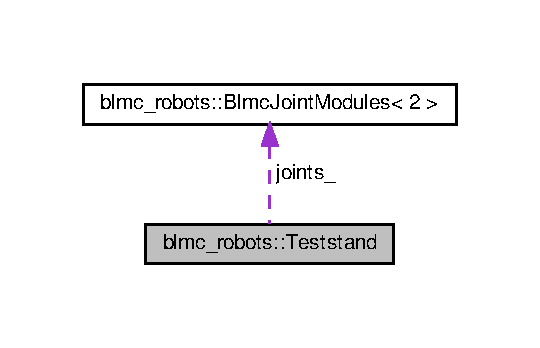
\includegraphics[width=259pt]{classblmc__robots_1_1Teststand__coll__graph}
\end{center}
\end{figure}
\subsection*{Public Types}
\begin{DoxyCompactItemize}
\item 
\mbox{\Hypertarget{classblmc__robots_1_1Teststand_a201214fc01f68b97ceba62af3fb8cccf}\label{classblmc__robots_1_1Teststand_a201214fc01f68b97ceba62af3fb8cccf}} 
typedef Eigen\+::\+Matrix$<$ double, 2, 1 $>$ \hyperlink{classblmc__robots_1_1Teststand_a201214fc01f68b97ceba62af3fb8cccf}{Vector\+Slider}
\begin{DoxyCompactList}\small\item\em Data type containing the \hyperlink{classblmc__robots_1_1Sliders}{Sliders} data. \end{DoxyCompactList}\item 
\mbox{\Hypertarget{classblmc__robots_1_1Teststand_a23b0a73bc99ce4a3588204b7480eb6d7}\label{classblmc__robots_1_1Teststand_a23b0a73bc99ce4a3588204b7480eb6d7}} 
typedef Eigen\+::\+Matrix$<$ double, 1, 1 $>$ \hyperlink{classblmc__robots_1_1Teststand_a23b0a73bc99ce4a3588204b7480eb6d7}{Vector\+Contact}
\begin{DoxyCompactList}\small\item\em This represents the contact sensor. \end{DoxyCompactList}\item 
\mbox{\Hypertarget{classblmc__robots_1_1Teststand_a51f17cf2b01dd8252e21db97b486e067}\label{classblmc__robots_1_1Teststand_a51f17cf2b01dd8252e21db97b486e067}} 
typedef Eigen\+::\+Matrix$<$ double, 3, 1 $>$ \hyperlink{classblmc__robots_1_1Teststand_a51f17cf2b01dd8252e21db97b486e067}{Vector\+Ati\+Force}
\begin{DoxyCompactList}\small\item\em This type define the forces from the ati-\/\+FT sensors. \end{DoxyCompactList}\item 
\mbox{\Hypertarget{classblmc__robots_1_1Teststand_a466977786f9b007854fa2eb2a97b0de9}\label{classblmc__robots_1_1Teststand_a466977786f9b007854fa2eb2a97b0de9}} 
typedef Eigen\+::\+Matrix$<$ double, 3, 1 $>$ \hyperlink{classblmc__robots_1_1Teststand_a466977786f9b007854fa2eb2a97b0de9}{Vector\+Ati\+Torque}
\begin{DoxyCompactList}\small\item\em This type define the torqes from the ati-\/\+FT sensors. \end{DoxyCompactList}\end{DoxyCompactItemize}
\subsection*{Public Member Functions}
\begin{DoxyCompactItemize}
\item 
\hyperlink{classblmc__robots_1_1Teststand_a4747b0754cd3dd669c02f27662baef7e}{Teststand} ()
\begin{DoxyCompactList}\small\item\em \hyperlink{classblmc__robots_1_1Teststand}{Teststand} is the constructor of the class. \end{DoxyCompactList}\item 
\mbox{\Hypertarget{classblmc__robots_1_1Teststand_aa41ad951a8259fd15e6309e850a6084a}\label{classblmc__robots_1_1Teststand_aa41ad951a8259fd15e6309e850a6084a}} 
void \hyperlink{classblmc__robots_1_1Teststand_aa41ad951a8259fd15e6309e850a6084a}{initialize} ()
\begin{DoxyCompactList}\small\item\em initialize the robot by setting aligning the motors and calibrate the sensors to 0 \end{DoxyCompactList}\item 
\mbox{\Hypertarget{classblmc__robots_1_1Teststand_aabb484d65bca5a341dd24abd91c47b9b}\label{classblmc__robots_1_1Teststand_aabb484d65bca5a341dd24abd91c47b9b}} 
bool \hyperlink{classblmc__robots_1_1Teststand_aabb484d65bca5a341dd24abd91c47b9b}{send\+\_\+target\+\_\+joint\+\_\+torque} (const Eigen\+::\+Ref$<$ \hyperlink{common__header_8hpp_acb6916bc8c9fe9d98c484fd4cc201447}{Vector2d} $>$ target\+\_\+joint\+\_\+torque)
\begin{DoxyCompactList}\small\item\em send\+\_\+target\+\_\+torques sends the target currents to the motors \end{DoxyCompactList}\item 
bool \hyperlink{classblmc__robots_1_1Teststand_a4203e25148ab5b4ddfef3b46647213c6}{acquire\+\_\+sensors} ()
\begin{DoxyCompactList}\small\item\em acquire\+\_\+sensors acquire all available sensors, W\+A\+R\+N\+I\+NG !!!! this method has to be called prior to any getter to have up to date data. \end{DoxyCompactList}\item 
bool \hyperlink{classblmc__robots_1_1Teststand_ad4660570e3e1b77717004b3ce8056faf}{calibrate} (const \hyperlink{common__header_8hpp_acb6916bc8c9fe9d98c484fd4cc201447}{Vector2d} \&home\+\_\+offset\+\_\+rad)
\begin{DoxyCompactList}\small\item\em This function will run a small controller that will move the joints untils the next joint index and reset the joint zero with this knowledge. \end{DoxyCompactList}\item 
const Eigen\+::\+Ref$<$ \hyperlink{common__header_8hpp_acb6916bc8c9fe9d98c484fd4cc201447}{Vector2d} $>$ \hyperlink{classblmc__robots_1_1Teststand_a4897109730380ae0be7da37e2bd69e81}{get\+\_\+motor\+\_\+inertias} ()
\begin{DoxyCompactList}\small\item\em get\+\_\+motor\+\_\+inertias \end{DoxyCompactList}\item 
const Eigen\+::\+Ref$<$ \hyperlink{common__header_8hpp_acb6916bc8c9fe9d98c484fd4cc201447}{Vector2d} $>$ \hyperlink{classblmc__robots_1_1Teststand_a483bc937ac8c95b93bb90c47744da2e8}{get\+\_\+motor\+\_\+torque\+\_\+constants} ()
\begin{DoxyCompactList}\small\item\em get\+\_\+motor\+\_\+torque\+\_\+constants \end{DoxyCompactList}\item 
const Eigen\+::\+Ref$<$ \hyperlink{common__header_8hpp_acb6916bc8c9fe9d98c484fd4cc201447}{Vector2d} $>$ \hyperlink{classblmc__robots_1_1Teststand_adf08db3dbb4fd8da74c8ef15fb393c1a}{get\+\_\+joint\+\_\+positions} ()
\begin{DoxyCompactList}\small\item\em get\+\_\+joint\+\_\+positions W\+A\+R\+N\+I\+NG !!!! The method \hyperlink{classblmc__robots_1_1Teststand_a4203e25148ab5b4ddfef3b46647213c6}{acquire\+\_\+sensors()} has to be called prior to any getter to have up to date data. \end{DoxyCompactList}\item 
const Eigen\+::\+Ref$<$ \hyperlink{common__header_8hpp_acb6916bc8c9fe9d98c484fd4cc201447}{Vector2d} $>$ \hyperlink{classblmc__robots_1_1Teststand_acd1b325c6039fffbd40198f6deb9542c}{get\+\_\+joint\+\_\+velocities} ()
\begin{DoxyCompactList}\small\item\em get\+\_\+joint\+\_\+velocities W\+A\+R\+N\+I\+NG !!!! The method \hyperlink{classblmc__robots_1_1Teststand_a4203e25148ab5b4ddfef3b46647213c6}{acquire\+\_\+sensors()} has to be called prior to any getter to have up to date data. \end{DoxyCompactList}\item 
const Eigen\+::\+Ref$<$ \hyperlink{common__header_8hpp_acb6916bc8c9fe9d98c484fd4cc201447}{Vector2d} $>$ \hyperlink{classblmc__robots_1_1Teststand_ae21ac86534e5ee7f15068f94957ba826}{get\+\_\+joint\+\_\+torques} ()
\begin{DoxyCompactList}\small\item\em get\+\_\+joint\+\_\+torques W\+A\+R\+N\+I\+NG !!!! The method \hyperlink{classblmc__robots_1_1Teststand_a4203e25148ab5b4ddfef3b46647213c6}{acquire\+\_\+sensors()} has to be called prior to any getter to have up to date data. \end{DoxyCompactList}\item 
const Eigen\+::\+Ref$<$ \hyperlink{common__header_8hpp_acb6916bc8c9fe9d98c484fd4cc201447}{Vector2d} $>$ \hyperlink{classblmc__robots_1_1Teststand_a0aa762511624791e4ccbec5ad664371f}{get\+\_\+joint\+\_\+target\+\_\+torques} ()
\begin{DoxyCompactList}\small\item\em get\+\_\+joint\+\_\+torques \end{DoxyCompactList}\item 
const Eigen\+::\+Ref$<$ \hyperlink{common__header_8hpp_acb6916bc8c9fe9d98c484fd4cc201447}{Vector2d} $>$ \hyperlink{classblmc__robots_1_1Teststand_a7def64b82a1cb58c9ae8c9c54bcaa887}{get\+\_\+joint\+\_\+gear\+\_\+ratios} ()
\begin{DoxyCompactList}\small\item\em get\+\_\+joint\+\_\+gear\+\_\+ratios \end{DoxyCompactList}\item 
const Eigen\+::\+Ref$<$ \hyperlink{common__header_8hpp_acb6916bc8c9fe9d98c484fd4cc201447}{Vector2d} $>$ \hyperlink{classblmc__robots_1_1Teststand_a2fa7aacb213c7898bb04f791ca3687d1}{get\+\_\+joint\+\_\+encoder\+\_\+index} ()
\begin{DoxyCompactList}\small\item\em get\+\_\+joint\+\_\+encoder\+\_\+index W\+A\+R\+N\+I\+NG !!!! The method \hyperlink{classblmc__robots_1_1Teststand_a4203e25148ab5b4ddfef3b46647213c6}{acquire\+\_\+sensors()} has to be called prior to any getter to have up to date data. \end{DoxyCompactList}\item 
const Eigen\+::\+Ref$<$ \hyperlink{common__header_8hpp_acb6916bc8c9fe9d98c484fd4cc201447}{Vector2d} $>$ \hyperlink{classblmc__robots_1_1Teststand_adbceb17de729cced8e9985b9177efa7c}{get\+\_\+zero\+\_\+positions} ()
\begin{DoxyCompactList}\small\item\em get\+\_\+zero\+\_\+positions \end{DoxyCompactList}\item 
const Eigen\+::\+Ref$<$ \hyperlink{common__header_8hpp_acb6916bc8c9fe9d98c484fd4cc201447}{Vector2d} $>$ \hyperlink{classblmc__robots_1_1Teststand_af46acfc1bd408d40b850c4780e834f53}{get\+\_\+slider\+\_\+positions} ()
\begin{DoxyCompactList}\small\item\em get\+\_\+slider\+\_\+positions W\+A\+R\+N\+I\+NG !!!! The method \hyperlink{classblmc__robots_1_1Teststand_a4203e25148ab5b4ddfef3b46647213c6}{acquire\+\_\+sensors()} has to be called prior to any getter to have up to date data. \end{DoxyCompactList}\item 
const Eigen\+::\+Ref$<$ \hyperlink{common__header_8hpp_a932c1319d78144ebcaa8938ae070b784}{Vector1d} $>$ \hyperlink{classblmc__robots_1_1Teststand_a0486afbd05d4f7c354ebad8432c178bd}{get\+\_\+contact\+\_\+sensors\+\_\+states} ()
\begin{DoxyCompactList}\small\item\em get\+\_\+contact\+\_\+sensors\+\_\+states W\+A\+R\+N\+I\+NG !!!! The method \hyperlink{classblmc__robots_1_1Teststand_a4203e25148ab5b4ddfef3b46647213c6}{acquire\+\_\+sensors()} has to be called prior to any getter to have up to date data. \end{DoxyCompactList}\item 
const Eigen\+::\+Ref$<$ \hyperlink{common__header_8hpp_a932c1319d78144ebcaa8938ae070b784}{Vector1d} $>$ \hyperlink{classblmc__robots_1_1Teststand_af8a0d1cc608f91a0a752758c7554087a}{get\+\_\+height\+\_\+sensors} ()
\begin{DoxyCompactList}\small\item\em get\+\_\+contact\+\_\+sensors\+\_\+states W\+A\+R\+N\+I\+NG !!!! The method \hyperlink{classblmc__robots_1_1Teststand_a4203e25148ab5b4ddfef3b46647213c6}{acquire\+\_\+sensors()} has to be called prior to any getter to have up to date data. \end{DoxyCompactList}\item 
const Eigen\+::\+Ref$<$ \hyperlink{common__header_8hpp_acb6916bc8c9fe9d98c484fd4cc201447}{Vector2d} $>$ \hyperlink{classblmc__robots_1_1Teststand_a2f912631ee055e3909ef1a5e06d8d27c}{get\+\_\+max\+\_\+current} ()
\begin{DoxyCompactList}\small\item\em get\+\_\+max\+\_\+current \end{DoxyCompactList}\item 
const Eigen\+::\+Ref$<$ \hyperlink{classblmc__robots_1_1Teststand_a51f17cf2b01dd8252e21db97b486e067}{Vector\+Ati\+Force} $>$ \hyperlink{classblmc__robots_1_1Teststand_af4bf3a4692fdeacdad78a7213c3fbe98}{get\+\_\+ati\+\_\+force} ()
\begin{DoxyCompactList}\small\item\em Get the ati\+\_\+force\+\_\+ object W\+A\+R\+N\+I\+NG !!!! The method \hyperlink{classblmc__robots_1_1Teststand_a4203e25148ab5b4ddfef3b46647213c6}{acquire\+\_\+sensors()} has to be called prior to any getter to have up to date data. \end{DoxyCompactList}\item 
const Eigen\+::\+Ref$<$ \hyperlink{classblmc__robots_1_1Teststand_a466977786f9b007854fa2eb2a97b0de9}{Vector\+Ati\+Torque} $>$ \hyperlink{classblmc__robots_1_1Teststand_a27ba45a099b4ff6852f5acd0226aa915}{get\+\_\+ati\+\_\+torque} ()
\begin{DoxyCompactList}\small\item\em Get the ati\+\_\+torque\+\_\+ object W\+A\+R\+N\+I\+NG !!!! The method \hyperlink{classblmc__robots_1_1Teststand_a4203e25148ab5b4ddfef3b46647213c6}{acquire\+\_\+sensors()} has to be called prior to any getter to have up to date data. \end{DoxyCompactList}\end{DoxyCompactItemize}
\subsection*{Private Attributes}
\begin{DoxyCompactItemize}
\item 
\mbox{\Hypertarget{classblmc__robots_1_1Teststand_ac733828512ab4ba2ad43625915a4a9fd}\label{classblmc__robots_1_1Teststand_ac733828512ab4ba2ad43625915a4a9fd}} 
ati\+\_\+ft\+\_\+sensor\+::\+Ati\+F\+T\+Sensor \hyperlink{classblmc__robots_1_1Teststand_ac733828512ab4ba2ad43625915a4a9fd}{ati\+\_\+sensor\+\_\+}
\begin{DoxyCompactList}\small\item\em A\+TI sensor. \end{DoxyCompactList}\item 
\mbox{\Hypertarget{classblmc__robots_1_1Teststand_abbde43d983602e1ead15b1b525cc524f}\label{classblmc__robots_1_1Teststand_abbde43d983602e1ead15b1b525cc524f}} 
\hyperlink{classblmc__robots_1_1Teststand_a51f17cf2b01dd8252e21db97b486e067}{Vector\+Ati\+Force} \hyperlink{classblmc__robots_1_1Teststand_abbde43d983602e1ead15b1b525cc524f}{ati\+\_\+force\+\_\+}
\begin{DoxyCompactList}\small\item\em 3D linear force from the A\+TI FT sensor \end{DoxyCompactList}\item 
\mbox{\Hypertarget{classblmc__robots_1_1Teststand_a8c4e095818a0c80739a63a91bb0670c6}\label{classblmc__robots_1_1Teststand_a8c4e095818a0c80739a63a91bb0670c6}} 
\hyperlink{classblmc__robots_1_1Teststand_a466977786f9b007854fa2eb2a97b0de9}{Vector\+Ati\+Torque} \hyperlink{classblmc__robots_1_1Teststand_a8c4e095818a0c80739a63a91bb0670c6}{ati\+\_\+torque\+\_\+}
\begin{DoxyCompactList}\small\item\em 3D torque measured from the A\+TI FT sensor \end{DoxyCompactList}\item 
\hyperlink{common__header_8hpp_acb6916bc8c9fe9d98c484fd4cc201447}{Vector2d} \hyperlink{classblmc__robots_1_1Teststand_afe8801388760cd85771a99e3a89c9f69}{motor\+\_\+inertias\+\_\+}
\begin{DoxyCompactList}\small\item\em Motor data. \end{DoxyCompactList}\item 
\mbox{\Hypertarget{classblmc__robots_1_1Teststand_a0d4bfad1f7afaaf459131667fac2b2d0}\label{classblmc__robots_1_1Teststand_a0d4bfad1f7afaaf459131667fac2b2d0}} 
\hyperlink{common__header_8hpp_acb6916bc8c9fe9d98c484fd4cc201447}{Vector2d} \hyperlink{classblmc__robots_1_1Teststand_a0d4bfad1f7afaaf459131667fac2b2d0}{motor\+\_\+torque\+\_\+constants\+\_\+}
\begin{DoxyCompactList}\small\item\em motor\+\_\+torque\+\_\+constants\+\_\+ are the motor torque constants \end{DoxyCompactList}\item 
\hyperlink{common__header_8hpp_acb6916bc8c9fe9d98c484fd4cc201447}{Vector2d} \hyperlink{classblmc__robots_1_1Teststand_a5ff6d1081ece6fadf9b3bac578b08001}{joint\+\_\+positions\+\_\+}
\begin{DoxyCompactList}\small\item\em Joint data. \end{DoxyCompactList}\item 
\mbox{\Hypertarget{classblmc__robots_1_1Teststand_ab0a776f921bec24b81bc08f7ceebcba6}\label{classblmc__robots_1_1Teststand_ab0a776f921bec24b81bc08f7ceebcba6}} 
\hyperlink{common__header_8hpp_acb6916bc8c9fe9d98c484fd4cc201447}{Vector2d} \hyperlink{classblmc__robots_1_1Teststand_ab0a776f921bec24b81bc08f7ceebcba6}{joint\+\_\+velocities\+\_\+}
\begin{DoxyCompactList}\small\item\em joint\+\_\+velocities\+\_\+ is the measured data from the onboard card converted at the joint level. \end{DoxyCompactList}\item 
\mbox{\Hypertarget{classblmc__robots_1_1Teststand_a59ef3d86efd043ee1511bad70624bdae}\label{classblmc__robots_1_1Teststand_a59ef3d86efd043ee1511bad70624bdae}} 
\hyperlink{common__header_8hpp_acb6916bc8c9fe9d98c484fd4cc201447}{Vector2d} \hyperlink{classblmc__robots_1_1Teststand_a59ef3d86efd043ee1511bad70624bdae}{joint\+\_\+torques\+\_\+}
\begin{DoxyCompactList}\small\item\em joint\+\_\+torques\+\_\+ is the measured data from the onboard card converted at the joint level. \end{DoxyCompactList}\item 
\mbox{\Hypertarget{classblmc__robots_1_1Teststand_a0db888b3e84fe194629bb14b6fa2e485}\label{classblmc__robots_1_1Teststand_a0db888b3e84fe194629bb14b6fa2e485}} 
\hyperlink{common__header_8hpp_acb6916bc8c9fe9d98c484fd4cc201447}{Vector2d} \hyperlink{classblmc__robots_1_1Teststand_a0db888b3e84fe194629bb14b6fa2e485}{joint\+\_\+target\+\_\+torques\+\_\+}
\begin{DoxyCompactList}\small\item\em joint\+\_\+target\+\_\+torques\+\_\+ is the last given command to be sent. \end{DoxyCompactList}\item 
\mbox{\Hypertarget{classblmc__robots_1_1Teststand_ad7b3b6c032d1b1b9c886089ea21a9c2a}\label{classblmc__robots_1_1Teststand_ad7b3b6c032d1b1b9c886089ea21a9c2a}} 
\hyperlink{common__header_8hpp_acb6916bc8c9fe9d98c484fd4cc201447}{Vector2d} \hyperlink{classblmc__robots_1_1Teststand_ad7b3b6c032d1b1b9c886089ea21a9c2a}{joint\+\_\+gear\+\_\+ratios\+\_\+}
\begin{DoxyCompactList}\small\item\em joint\+\_\+gear\+\_\+ratios are the joint gear ratios \end{DoxyCompactList}\item 
\mbox{\Hypertarget{classblmc__robots_1_1Teststand_a2a0b967c36ea63a8bb564bdeebcc0846}\label{classblmc__robots_1_1Teststand_a2a0b967c36ea63a8bb564bdeebcc0846}} 
\hyperlink{common__header_8hpp_acb6916bc8c9fe9d98c484fd4cc201447}{Vector2d} \hyperlink{classblmc__robots_1_1Teststand_a2a0b967c36ea63a8bb564bdeebcc0846}{joint\+\_\+encoder\+\_\+index\+\_\+}
\begin{DoxyCompactList}\small\item\em joint\+\_\+encoder\+\_\+index\+\_\+ The last observed encoder\+\_\+index at the joints. \end{DoxyCompactList}\item 
\mbox{\Hypertarget{classblmc__robots_1_1Teststand_a5923674652df619a0692333fb27b8369}\label{classblmc__robots_1_1Teststand_a5923674652df619a0692333fb27b8369}} 
\hyperlink{common__header_8hpp_acb6916bc8c9fe9d98c484fd4cc201447}{Vector2d} \hyperlink{classblmc__robots_1_1Teststand_a5923674652df619a0692333fb27b8369}{joint\+\_\+zero\+\_\+positions\+\_\+}
\begin{DoxyCompactList}\small\item\em joint\+\_\+zero\+\_\+positions\+\_\+ is the configuration considered as zero position \end{DoxyCompactList}\item 
\hyperlink{common__header_8hpp_acb6916bc8c9fe9d98c484fd4cc201447}{Vector2d} \hyperlink{classblmc__robots_1_1Teststand_ad0ce099eef5b57553d36927e3f7f1203}{slider\+\_\+positions\+\_\+}
\begin{DoxyCompactList}\small\item\em Additional data. \end{DoxyCompactList}\item 
\mbox{\Hypertarget{classblmc__robots_1_1Teststand_a49bb3cd738af64ef41a9a3d12dde9ac2}\label{classblmc__robots_1_1Teststand_a49bb3cd738af64ef41a9a3d12dde9ac2}} 
\hyperlink{common__header_8hpp_a932c1319d78144ebcaa8938ae070b784}{Vector1d} \hyperlink{classblmc__robots_1_1Teststand_a49bb3cd738af64ef41a9a3d12dde9ac2}{contact\+\_\+sensors\+\_\+states\+\_\+}
\begin{DoxyCompactList}\small\item\em contact\+\_\+sensors\+\_\+ is contact sensors at the foot \end{DoxyCompactList}\item 
\mbox{\Hypertarget{classblmc__robots_1_1Teststand_af9c7f9537b7123dae498d08d5c80fe07}\label{classblmc__robots_1_1Teststand_af9c7f9537b7123dae498d08d5c80fe07}} 
\hyperlink{common__header_8hpp_a932c1319d78144ebcaa8938ae070b784}{Vector1d} \hyperlink{classblmc__robots_1_1Teststand_af9c7f9537b7123dae498d08d5c80fe07}{height\+\_\+sensors\+\_\+states\+\_\+}
\begin{DoxyCompactList}\small\item\em height\+\_\+sensors\+\_\+ is the height position of the base. \end{DoxyCompactList}\item 
\mbox{\Hypertarget{classblmc__robots_1_1Teststand_aae2cff55630f887e4ed10af78b7dd0c1}\label{classblmc__robots_1_1Teststand_aae2cff55630f887e4ed10af78b7dd0c1}} 
\hyperlink{common__header_8hpp_acb6916bc8c9fe9d98c484fd4cc201447}{Vector2d} \hyperlink{classblmc__robots_1_1Teststand_aae2cff55630f887e4ed10af78b7dd0c1}{motor\+\_\+max\+\_\+current\+\_\+}
\begin{DoxyCompactList}\small\item\em max\+\_\+current\+\_\+ is the maximum current that can be sent to the motors, this a safe guard for development \end{DoxyCompactList}\item 
\mbox{\Hypertarget{classblmc__robots_1_1Teststand_acf65e7889b3c8b3cbfa8b9e82e984b22}\label{classblmc__robots_1_1Teststand_acf65e7889b3c8b3cbfa8b9e82e984b22}} 
Eigen\+::\+Array2d \hyperlink{classblmc__robots_1_1Teststand_acf65e7889b3c8b3cbfa8b9e82e984b22}{max\+\_\+joint\+\_\+torques\+\_\+}
\begin{DoxyCompactList}\small\item\em max\+\_\+joint\+\_\+torques\+\_\+ (Nm) \end{DoxyCompactList}\item 
\mbox{\Hypertarget{classblmc__robots_1_1Teststand_aedd9aae28f47062870e3afcb9474822b}\label{classblmc__robots_1_1Teststand_aedd9aae28f47062870e3afcb9474822b}} 
std\+::array$<$ bool, 4 $>$ \hyperlink{classblmc__robots_1_1Teststand_aedd9aae28f47062870e3afcb9474822b}{motor\+\_\+enabled\+\_\+}
\begin{DoxyCompactList}\small\item\em This gives the status (enabled/disabled) of each motors using the joint ordering convention. \end{DoxyCompactList}\item 
\mbox{\Hypertarget{classblmc__robots_1_1Teststand_a62df6b43c18e44f62114b6f4d34ba8f4}\label{classblmc__robots_1_1Teststand_a62df6b43c18e44f62114b6f4d34ba8f4}} 
std\+::array$<$ bool, 4 $>$ \hyperlink{classblmc__robots_1_1Teststand_a62df6b43c18e44f62114b6f4d34ba8f4}{motor\+\_\+ready\+\_\+}
\begin{DoxyCompactList}\small\item\em This gives the status (enabled/disabled) of each motors using the joint ordering convention. \end{DoxyCompactList}\item 
\mbox{\Hypertarget{classblmc__robots_1_1Teststand_a1fca1e72202c09982c2e77c3166d1ea7}\label{classblmc__robots_1_1Teststand_a1fca1e72202c09982c2e77c3166d1ea7}} 
std\+::array$<$ bool, 2 $>$ \hyperlink{classblmc__robots_1_1Teststand_a1fca1e72202c09982c2e77c3166d1ea7}{motor\+\_\+board\+\_\+enabled\+\_\+}
\begin{DoxyCompactList}\small\item\em This gives the status (enabled/disabled of the onboard control cards) \end{DoxyCompactList}\item 
\mbox{\Hypertarget{classblmc__robots_1_1Teststand_a89f931457834d37bd01da57944fd21c1}\label{classblmc__robots_1_1Teststand_a89f931457834d37bd01da57944fd21c1}} 
std\+::array$<$ int, 2 $>$ \hyperlink{classblmc__robots_1_1Teststand_a89f931457834d37bd01da57944fd21c1}{motor\+\_\+board\+\_\+errors\+\_\+}
\begin{DoxyCompactList}\small\item\em This gives the status (enabled/disabled of the onboard control cards) \end{DoxyCompactList}\item 
std\+::array$<$ \hyperlink{common__header_8hpp_a793c8789a7598e8aaf766939da7262af}{Can\+Bus\+\_\+ptr}, 2 $>$ \hyperlink{classblmc__robots_1_1Teststand_aab9d6924ad67f65a6931d3db4771c28a}{can\+\_\+buses\+\_\+}
\begin{DoxyCompactList}\small\item\em Drivers communication objects. \end{DoxyCompactList}\item 
\mbox{\Hypertarget{classblmc__robots_1_1Teststand_a5ab181273e83c54a66ece2f741b718bb}\label{classblmc__robots_1_1Teststand_a5ab181273e83c54a66ece2f741b718bb}} 
std\+::array$<$ \hyperlink{common__header_8hpp_aab1c6ddb1273247a1b45d5e8b417c216}{Can\+Bus\+Motor\+Board\+\_\+ptr}, 2 $>$ \hyperlink{classblmc__robots_1_1Teststand_a5ab181273e83c54a66ece2f741b718bb}{can\+\_\+motor\+\_\+boards\+\_\+}
\begin{DoxyCompactList}\small\item\em can\+\_\+motor\+\_\+boards\+\_\+ are the 2 can motor board. \end{DoxyCompactList}\item 
\mbox{\Hypertarget{classblmc__robots_1_1Teststand_ae530206f8c54cbc04d7cf69a16d1e99a}\label{classblmc__robots_1_1Teststand_ae530206f8c54cbc04d7cf69a16d1e99a}} 
std\+::array$<$ \hyperlink{common__header_8hpp_ae1a0f9992bc8fbbc1943d887f517c180}{Motor\+Interface\+\_\+ptr}, 2 $>$ \hyperlink{classblmc__robots_1_1Teststand_ae530206f8c54cbc04d7cf69a16d1e99a}{motors\+\_\+}
\begin{DoxyCompactList}\small\item\em motors\+\_\+ are the objects allowing us to send motor commands and receive data \end{DoxyCompactList}\item 
\hyperlink{classblmc__robots_1_1BlmcJointModules}{Blmc\+Joint\+Modules}$<$ 2 $>$ \hyperlink{classblmc__robots_1_1Teststand_a2c14882d88deb56edde5240a8d841f2a}{joints\+\_\+}
\begin{DoxyCompactList}\small\item\em joint\+\_\+ptrs\+\_\+ are the objects allowing us to send commands and receive data at the joint level. \end{DoxyCompactList}\item 
\mbox{\Hypertarget{classblmc__robots_1_1Teststand_a2a67df9dc9004f9e70bcdd6ad8f8189e}\label{classblmc__robots_1_1Teststand_a2a67df9dc9004f9e70bcdd6ad8f8189e}} 
std\+::array$<$ \hyperlink{common__header_8hpp_a4cb9a95e8b2c0bf237ce29f5252c7b73}{Slider\+\_\+ptr}, 2 $>$ \hyperlink{classblmc__robots_1_1Teststand_a2a67df9dc9004f9e70bcdd6ad8f8189e}{sliders\+\_\+}
\begin{DoxyCompactList}\small\item\em sliders\+\_\+ these are analogue input from linear potentiometers. \end{DoxyCompactList}\item 
std\+::array$<$ \hyperlink{common__header_8hpp_ac78fe5c68e56a3b884117109959e4d58}{Contact\+Sensor\+\_\+ptr}, 1 $>$ \hyperlink{classblmc__robots_1_1Teststand_af2f14b46da7f2dfbeeea59b47669f1e8}{contact\+\_\+sensors\+\_\+}
\begin{DoxyCompactList}\small\item\em contact\+\_\+sensors\+\_\+ is the contact sensors at each foot tips. \end{DoxyCompactList}\item 
std\+::array$<$ \hyperlink{common__header_8hpp_a921d3f5a8878524375bf7e740f2fb788}{Height\+Sensor\+\_\+ptr}, 1 $>$ \hyperlink{classblmc__robots_1_1Teststand_a41a93d1d128333a9981603eb82d068c0}{height\+\_\+sensors\+\_\+}
\begin{DoxyCompactList}\small\item\em contact\+\_\+sensors\+\_\+ is the contact sensors at each foot tips. \end{DoxyCompactList}\end{DoxyCompactItemize}
\subsection*{Static Private Attributes}
\begin{DoxyCompactItemize}
\item 
\mbox{\Hypertarget{classblmc__robots_1_1Teststand_a401728dd5ba91b8603de79125fcb0a66}\label{classblmc__robots_1_1Teststand_a401728dd5ba91b8603de79125fcb0a66}} 
static const double \hyperlink{classblmc__robots_1_1Teststand_a401728dd5ba91b8603de79125fcb0a66}{max\+\_\+joint\+\_\+torque\+\_\+security\+\_\+margin\+\_\+} = 0.\+99
\begin{DoxyCompactList}\small\item\em Security margin on the saturation of the control. \end{DoxyCompactList}\end{DoxyCompactItemize}


\subsection{Detailed Description}
The class \hyperlink{classblmc__robots_1_1Teststand}{Teststand} is used to control the \hyperlink{classblmc__robots_1_1Teststand}{Teststand} robot located at M\+P\+I-\/\+IS Tuebingen. 

The robot is composed of a single leg on a vertical rail. 

\subsection{Constructor \& Destructor Documentation}
\mbox{\Hypertarget{classblmc__robots_1_1Teststand_a4747b0754cd3dd669c02f27662baef7e}\label{classblmc__robots_1_1Teststand_a4747b0754cd3dd669c02f27662baef7e}} 
\index{blmc\+\_\+robots\+::\+Teststand@{blmc\+\_\+robots\+::\+Teststand}!Teststand@{Teststand}}
\index{Teststand@{Teststand}!blmc\+\_\+robots\+::\+Teststand@{blmc\+\_\+robots\+::\+Teststand}}
\subsubsection{\texorpdfstring{Teststand()}{Teststand()}}
{\footnotesize\ttfamily blmc\+\_\+robots\+::\+Teststand\+::\+Teststand (\begin{DoxyParamCaption}{ }\end{DoxyParamCaption})}



\hyperlink{classblmc__robots_1_1Teststand}{Teststand} is the constructor of the class. 

Motor data

Joint data

Additional data

Setup some known data

\subsection{Member Function Documentation}
\mbox{\Hypertarget{classblmc__robots_1_1Teststand_a4203e25148ab5b4ddfef3b46647213c6}\label{classblmc__robots_1_1Teststand_a4203e25148ab5b4ddfef3b46647213c6}} 
\index{blmc\+\_\+robots\+::\+Teststand@{blmc\+\_\+robots\+::\+Teststand}!acquire\+\_\+sensors@{acquire\+\_\+sensors}}
\index{acquire\+\_\+sensors@{acquire\+\_\+sensors}!blmc\+\_\+robots\+::\+Teststand@{blmc\+\_\+robots\+::\+Teststand}}
\subsubsection{\texorpdfstring{acquire\+\_\+sensors()}{acquire\_sensors()}}
{\footnotesize\ttfamily bool blmc\+\_\+robots\+::\+Teststand\+::acquire\+\_\+sensors (\begin{DoxyParamCaption}{ }\end{DoxyParamCaption})}



acquire\+\_\+sensors acquire all available sensors, W\+A\+R\+N\+I\+NG !!!! this method has to be called prior to any getter to have up to date data. 

Joint data

Additional data

Ati sensor readings.\mbox{\Hypertarget{classblmc__robots_1_1Teststand_ad4660570e3e1b77717004b3ce8056faf}\label{classblmc__robots_1_1Teststand_ad4660570e3e1b77717004b3ce8056faf}} 
\index{blmc\+\_\+robots\+::\+Teststand@{blmc\+\_\+robots\+::\+Teststand}!calibrate@{calibrate}}
\index{calibrate@{calibrate}!blmc\+\_\+robots\+::\+Teststand@{blmc\+\_\+robots\+::\+Teststand}}
\subsubsection{\texorpdfstring{calibrate()}{calibrate()}}
{\footnotesize\ttfamily bool blmc\+\_\+robots\+::\+Teststand\+::calibrate (\begin{DoxyParamCaption}\item[{const \hyperlink{common__header_8hpp_acb6916bc8c9fe9d98c484fd4cc201447}{Vector2d} \&}]{home\+\_\+offset\+\_\+rad }\end{DoxyParamCaption})}



This function will run a small controller that will move the joints untils the next joint index and reset the joint zero with this knowledge. 

\begin{DoxyReturn}{Returns}
true if success 

false if failure 
\end{DoxyReturn}
\mbox{\Hypertarget{classblmc__robots_1_1Teststand_af4bf3a4692fdeacdad78a7213c3fbe98}\label{classblmc__robots_1_1Teststand_af4bf3a4692fdeacdad78a7213c3fbe98}} 
\index{blmc\+\_\+robots\+::\+Teststand@{blmc\+\_\+robots\+::\+Teststand}!get\+\_\+ati\+\_\+force@{get\+\_\+ati\+\_\+force}}
\index{get\+\_\+ati\+\_\+force@{get\+\_\+ati\+\_\+force}!blmc\+\_\+robots\+::\+Teststand@{blmc\+\_\+robots\+::\+Teststand}}
\subsubsection{\texorpdfstring{get\+\_\+ati\+\_\+force()}{get\_ati\_force()}}
{\footnotesize\ttfamily const Eigen\+::\+Ref$<$\hyperlink{classblmc__robots_1_1Teststand_a51f17cf2b01dd8252e21db97b486e067}{Vector\+Ati\+Force}$>$ blmc\+\_\+robots\+::\+Teststand\+::get\+\_\+ati\+\_\+force (\begin{DoxyParamCaption}{ }\end{DoxyParamCaption})\hspace{0.3cm}{\ttfamily [inline]}}



Get the ati\+\_\+force\+\_\+ object W\+A\+R\+N\+I\+NG !!!! The method \hyperlink{classblmc__robots_1_1Teststand_a4203e25148ab5b4ddfef3b46647213c6}{acquire\+\_\+sensors()} has to be called prior to any getter to have up to date data. 

\begin{DoxyReturn}{Returns}
const Eigen\+::\+Ref$<$\+Vector\+Ati\+Force$>$ 
\end{DoxyReturn}
\mbox{\Hypertarget{classblmc__robots_1_1Teststand_a27ba45a099b4ff6852f5acd0226aa915}\label{classblmc__robots_1_1Teststand_a27ba45a099b4ff6852f5acd0226aa915}} 
\index{blmc\+\_\+robots\+::\+Teststand@{blmc\+\_\+robots\+::\+Teststand}!get\+\_\+ati\+\_\+torque@{get\+\_\+ati\+\_\+torque}}
\index{get\+\_\+ati\+\_\+torque@{get\+\_\+ati\+\_\+torque}!blmc\+\_\+robots\+::\+Teststand@{blmc\+\_\+robots\+::\+Teststand}}
\subsubsection{\texorpdfstring{get\+\_\+ati\+\_\+torque()}{get\_ati\_torque()}}
{\footnotesize\ttfamily const Eigen\+::\+Ref$<$\hyperlink{classblmc__robots_1_1Teststand_a466977786f9b007854fa2eb2a97b0de9}{Vector\+Ati\+Torque}$>$ blmc\+\_\+robots\+::\+Teststand\+::get\+\_\+ati\+\_\+torque (\begin{DoxyParamCaption}{ }\end{DoxyParamCaption})\hspace{0.3cm}{\ttfamily [inline]}}



Get the ati\+\_\+torque\+\_\+ object W\+A\+R\+N\+I\+NG !!!! The method \hyperlink{classblmc__robots_1_1Teststand_a4203e25148ab5b4ddfef3b46647213c6}{acquire\+\_\+sensors()} has to be called prior to any getter to have up to date data. 

\begin{DoxyReturn}{Returns}
const Eigen\+::\+Ref$<$\+Vector\+Ati\+Torque$>$ 
\end{DoxyReturn}
\mbox{\Hypertarget{classblmc__robots_1_1Teststand_a0486afbd05d4f7c354ebad8432c178bd}\label{classblmc__robots_1_1Teststand_a0486afbd05d4f7c354ebad8432c178bd}} 
\index{blmc\+\_\+robots\+::\+Teststand@{blmc\+\_\+robots\+::\+Teststand}!get\+\_\+contact\+\_\+sensors\+\_\+states@{get\+\_\+contact\+\_\+sensors\+\_\+states}}
\index{get\+\_\+contact\+\_\+sensors\+\_\+states@{get\+\_\+contact\+\_\+sensors\+\_\+states}!blmc\+\_\+robots\+::\+Teststand@{blmc\+\_\+robots\+::\+Teststand}}
\subsubsection{\texorpdfstring{get\+\_\+contact\+\_\+sensors\+\_\+states()}{get\_contact\_sensors\_states()}}
{\footnotesize\ttfamily const Eigen\+::\+Ref$<$\hyperlink{common__header_8hpp_a932c1319d78144ebcaa8938ae070b784}{Vector1d}$>$ blmc\+\_\+robots\+::\+Teststand\+::get\+\_\+contact\+\_\+sensors\+\_\+states (\begin{DoxyParamCaption}{ }\end{DoxyParamCaption})\hspace{0.3cm}{\ttfamily [inline]}}



get\+\_\+contact\+\_\+sensors\+\_\+states W\+A\+R\+N\+I\+NG !!!! The method \hyperlink{classblmc__robots_1_1Teststand_a4203e25148ab5b4ddfef3b46647213c6}{acquire\+\_\+sensors()} has to be called prior to any getter to have up to date data. 

\begin{DoxyReturn}{Returns}
the state of the contacts states 
\end{DoxyReturn}
\mbox{\Hypertarget{classblmc__robots_1_1Teststand_af8a0d1cc608f91a0a752758c7554087a}\label{classblmc__robots_1_1Teststand_af8a0d1cc608f91a0a752758c7554087a}} 
\index{blmc\+\_\+robots\+::\+Teststand@{blmc\+\_\+robots\+::\+Teststand}!get\+\_\+height\+\_\+sensors@{get\+\_\+height\+\_\+sensors}}
\index{get\+\_\+height\+\_\+sensors@{get\+\_\+height\+\_\+sensors}!blmc\+\_\+robots\+::\+Teststand@{blmc\+\_\+robots\+::\+Teststand}}
\subsubsection{\texorpdfstring{get\+\_\+height\+\_\+sensors()}{get\_height\_sensors()}}
{\footnotesize\ttfamily const Eigen\+::\+Ref$<$\hyperlink{common__header_8hpp_a932c1319d78144ebcaa8938ae070b784}{Vector1d}$>$ blmc\+\_\+robots\+::\+Teststand\+::get\+\_\+height\+\_\+sensors (\begin{DoxyParamCaption}{ }\end{DoxyParamCaption})\hspace{0.3cm}{\ttfamily [inline]}}



get\+\_\+contact\+\_\+sensors\+\_\+states W\+A\+R\+N\+I\+NG !!!! The method \hyperlink{classblmc__robots_1_1Teststand_a4203e25148ab5b4ddfef3b46647213c6}{acquire\+\_\+sensors()} has to be called prior to any getter to have up to date data. 

\begin{DoxyReturn}{Returns}
the state of the contacts states 
\end{DoxyReturn}
\mbox{\Hypertarget{classblmc__robots_1_1Teststand_a2fa7aacb213c7898bb04f791ca3687d1}\label{classblmc__robots_1_1Teststand_a2fa7aacb213c7898bb04f791ca3687d1}} 
\index{blmc\+\_\+robots\+::\+Teststand@{blmc\+\_\+robots\+::\+Teststand}!get\+\_\+joint\+\_\+encoder\+\_\+index@{get\+\_\+joint\+\_\+encoder\+\_\+index}}
\index{get\+\_\+joint\+\_\+encoder\+\_\+index@{get\+\_\+joint\+\_\+encoder\+\_\+index}!blmc\+\_\+robots\+::\+Teststand@{blmc\+\_\+robots\+::\+Teststand}}
\subsubsection{\texorpdfstring{get\+\_\+joint\+\_\+encoder\+\_\+index()}{get\_joint\_encoder\_index()}}
{\footnotesize\ttfamily const Eigen\+::\+Ref$<$\hyperlink{common__header_8hpp_acb6916bc8c9fe9d98c484fd4cc201447}{Vector2d}$>$ blmc\+\_\+robots\+::\+Teststand\+::get\+\_\+joint\+\_\+encoder\+\_\+index (\begin{DoxyParamCaption}{ }\end{DoxyParamCaption})\hspace{0.3cm}{\ttfamily [inline]}}



get\+\_\+joint\+\_\+encoder\+\_\+index W\+A\+R\+N\+I\+NG !!!! The method \hyperlink{classblmc__robots_1_1Teststand_a4203e25148ab5b4ddfef3b46647213c6}{acquire\+\_\+sensors()} has to be called prior to any getter to have up to date data. 

\begin{DoxyReturn}{Returns}
The last observed encoder index in joint coordinates. 
\end{DoxyReturn}
\mbox{\Hypertarget{classblmc__robots_1_1Teststand_a7def64b82a1cb58c9ae8c9c54bcaa887}\label{classblmc__robots_1_1Teststand_a7def64b82a1cb58c9ae8c9c54bcaa887}} 
\index{blmc\+\_\+robots\+::\+Teststand@{blmc\+\_\+robots\+::\+Teststand}!get\+\_\+joint\+\_\+gear\+\_\+ratios@{get\+\_\+joint\+\_\+gear\+\_\+ratios}}
\index{get\+\_\+joint\+\_\+gear\+\_\+ratios@{get\+\_\+joint\+\_\+gear\+\_\+ratios}!blmc\+\_\+robots\+::\+Teststand@{blmc\+\_\+robots\+::\+Teststand}}
\subsubsection{\texorpdfstring{get\+\_\+joint\+\_\+gear\+\_\+ratios()}{get\_joint\_gear\_ratios()}}
{\footnotesize\ttfamily const Eigen\+::\+Ref$<$\hyperlink{common__header_8hpp_acb6916bc8c9fe9d98c484fd4cc201447}{Vector2d}$>$ blmc\+\_\+robots\+::\+Teststand\+::get\+\_\+joint\+\_\+gear\+\_\+ratios (\begin{DoxyParamCaption}{ }\end{DoxyParamCaption})\hspace{0.3cm}{\ttfamily [inline]}}



get\+\_\+joint\+\_\+gear\+\_\+ratios 

\begin{DoxyReturn}{Returns}
the joint gear ratios 
\end{DoxyReturn}
\mbox{\Hypertarget{classblmc__robots_1_1Teststand_adf08db3dbb4fd8da74c8ef15fb393c1a}\label{classblmc__robots_1_1Teststand_adf08db3dbb4fd8da74c8ef15fb393c1a}} 
\index{blmc\+\_\+robots\+::\+Teststand@{blmc\+\_\+robots\+::\+Teststand}!get\+\_\+joint\+\_\+positions@{get\+\_\+joint\+\_\+positions}}
\index{get\+\_\+joint\+\_\+positions@{get\+\_\+joint\+\_\+positions}!blmc\+\_\+robots\+::\+Teststand@{blmc\+\_\+robots\+::\+Teststand}}
\subsubsection{\texorpdfstring{get\+\_\+joint\+\_\+positions()}{get\_joint\_positions()}}
{\footnotesize\ttfamily const Eigen\+::\+Ref$<$\hyperlink{common__header_8hpp_acb6916bc8c9fe9d98c484fd4cc201447}{Vector2d}$>$ blmc\+\_\+robots\+::\+Teststand\+::get\+\_\+joint\+\_\+positions (\begin{DoxyParamCaption}{ }\end{DoxyParamCaption})\hspace{0.3cm}{\ttfamily [inline]}}



get\+\_\+joint\+\_\+positions W\+A\+R\+N\+I\+NG !!!! The method \hyperlink{classblmc__robots_1_1Teststand_a4203e25148ab5b4ddfef3b46647213c6}{acquire\+\_\+sensors()} has to be called prior to any getter to have up to date data. 

\begin{DoxyReturn}{Returns}
the joint angle of each module 
\end{DoxyReturn}
\mbox{\Hypertarget{classblmc__robots_1_1Teststand_a0aa762511624791e4ccbec5ad664371f}\label{classblmc__robots_1_1Teststand_a0aa762511624791e4ccbec5ad664371f}} 
\index{blmc\+\_\+robots\+::\+Teststand@{blmc\+\_\+robots\+::\+Teststand}!get\+\_\+joint\+\_\+target\+\_\+torques@{get\+\_\+joint\+\_\+target\+\_\+torques}}
\index{get\+\_\+joint\+\_\+target\+\_\+torques@{get\+\_\+joint\+\_\+target\+\_\+torques}!blmc\+\_\+robots\+::\+Teststand@{blmc\+\_\+robots\+::\+Teststand}}
\subsubsection{\texorpdfstring{get\+\_\+joint\+\_\+target\+\_\+torques()}{get\_joint\_target\_torques()}}
{\footnotesize\ttfamily const Eigen\+::\+Ref$<$\hyperlink{common__header_8hpp_acb6916bc8c9fe9d98c484fd4cc201447}{Vector2d}$>$ blmc\+\_\+robots\+::\+Teststand\+::get\+\_\+joint\+\_\+target\+\_\+torques (\begin{DoxyParamCaption}{ }\end{DoxyParamCaption})\hspace{0.3cm}{\ttfamily [inline]}}



get\+\_\+joint\+\_\+torques 

\begin{DoxyReturn}{Returns}
the target joint torques 
\end{DoxyReturn}
\mbox{\Hypertarget{classblmc__robots_1_1Teststand_ae21ac86534e5ee7f15068f94957ba826}\label{classblmc__robots_1_1Teststand_ae21ac86534e5ee7f15068f94957ba826}} 
\index{blmc\+\_\+robots\+::\+Teststand@{blmc\+\_\+robots\+::\+Teststand}!get\+\_\+joint\+\_\+torques@{get\+\_\+joint\+\_\+torques}}
\index{get\+\_\+joint\+\_\+torques@{get\+\_\+joint\+\_\+torques}!blmc\+\_\+robots\+::\+Teststand@{blmc\+\_\+robots\+::\+Teststand}}
\subsubsection{\texorpdfstring{get\+\_\+joint\+\_\+torques()}{get\_joint\_torques()}}
{\footnotesize\ttfamily const Eigen\+::\+Ref$<$\hyperlink{common__header_8hpp_acb6916bc8c9fe9d98c484fd4cc201447}{Vector2d}$>$ blmc\+\_\+robots\+::\+Teststand\+::get\+\_\+joint\+\_\+torques (\begin{DoxyParamCaption}{ }\end{DoxyParamCaption})\hspace{0.3cm}{\ttfamily [inline]}}



get\+\_\+joint\+\_\+torques W\+A\+R\+N\+I\+NG !!!! The method \hyperlink{classblmc__robots_1_1Teststand_a4203e25148ab5b4ddfef3b46647213c6}{acquire\+\_\+sensors()} has to be called prior to any getter to have up to date data. 

\begin{DoxyReturn}{Returns}
the joint torques 
\end{DoxyReturn}
\mbox{\Hypertarget{classblmc__robots_1_1Teststand_acd1b325c6039fffbd40198f6deb9542c}\label{classblmc__robots_1_1Teststand_acd1b325c6039fffbd40198f6deb9542c}} 
\index{blmc\+\_\+robots\+::\+Teststand@{blmc\+\_\+robots\+::\+Teststand}!get\+\_\+joint\+\_\+velocities@{get\+\_\+joint\+\_\+velocities}}
\index{get\+\_\+joint\+\_\+velocities@{get\+\_\+joint\+\_\+velocities}!blmc\+\_\+robots\+::\+Teststand@{blmc\+\_\+robots\+::\+Teststand}}
\subsubsection{\texorpdfstring{get\+\_\+joint\+\_\+velocities()}{get\_joint\_velocities()}}
{\footnotesize\ttfamily const Eigen\+::\+Ref$<$\hyperlink{common__header_8hpp_acb6916bc8c9fe9d98c484fd4cc201447}{Vector2d}$>$ blmc\+\_\+robots\+::\+Teststand\+::get\+\_\+joint\+\_\+velocities (\begin{DoxyParamCaption}{ }\end{DoxyParamCaption})\hspace{0.3cm}{\ttfamily [inline]}}



get\+\_\+joint\+\_\+velocities W\+A\+R\+N\+I\+NG !!!! The method \hyperlink{classblmc__robots_1_1Teststand_a4203e25148ab5b4ddfef3b46647213c6}{acquire\+\_\+sensors()} has to be called prior to any getter to have up to date data. 

\begin{DoxyReturn}{Returns}
the joint velocities 
\end{DoxyReturn}
\mbox{\Hypertarget{classblmc__robots_1_1Teststand_a2f912631ee055e3909ef1a5e06d8d27c}\label{classblmc__robots_1_1Teststand_a2f912631ee055e3909ef1a5e06d8d27c}} 
\index{blmc\+\_\+robots\+::\+Teststand@{blmc\+\_\+robots\+::\+Teststand}!get\+\_\+max\+\_\+current@{get\+\_\+max\+\_\+current}}
\index{get\+\_\+max\+\_\+current@{get\+\_\+max\+\_\+current}!blmc\+\_\+robots\+::\+Teststand@{blmc\+\_\+robots\+::\+Teststand}}
\subsubsection{\texorpdfstring{get\+\_\+max\+\_\+current()}{get\_max\_current()}}
{\footnotesize\ttfamily const Eigen\+::\+Ref$<$\hyperlink{common__header_8hpp_acb6916bc8c9fe9d98c484fd4cc201447}{Vector2d}$>$ blmc\+\_\+robots\+::\+Teststand\+::get\+\_\+max\+\_\+current (\begin{DoxyParamCaption}{ }\end{DoxyParamCaption})\hspace{0.3cm}{\ttfamily [inline]}}



get\+\_\+max\+\_\+current 

\begin{DoxyReturn}{Returns}
the max current that has been hardcoded in the constructor of this class. T\+O\+DO\+: parametrize this via yaml or something else. 
\end{DoxyReturn}
\mbox{\Hypertarget{classblmc__robots_1_1Teststand_a4897109730380ae0be7da37e2bd69e81}\label{classblmc__robots_1_1Teststand_a4897109730380ae0be7da37e2bd69e81}} 
\index{blmc\+\_\+robots\+::\+Teststand@{blmc\+\_\+robots\+::\+Teststand}!get\+\_\+motor\+\_\+inertias@{get\+\_\+motor\+\_\+inertias}}
\index{get\+\_\+motor\+\_\+inertias@{get\+\_\+motor\+\_\+inertias}!blmc\+\_\+robots\+::\+Teststand@{blmc\+\_\+robots\+::\+Teststand}}
\subsubsection{\texorpdfstring{get\+\_\+motor\+\_\+inertias()}{get\_motor\_inertias()}}
{\footnotesize\ttfamily const Eigen\+::\+Ref$<$\hyperlink{common__header_8hpp_acb6916bc8c9fe9d98c484fd4cc201447}{Vector2d}$>$ blmc\+\_\+robots\+::\+Teststand\+::get\+\_\+motor\+\_\+inertias (\begin{DoxyParamCaption}{ }\end{DoxyParamCaption})\hspace{0.3cm}{\ttfamily [inline]}}



get\+\_\+motor\+\_\+inertias 

\begin{DoxyReturn}{Returns}
the motor inertias 
\end{DoxyReturn}
\mbox{\Hypertarget{classblmc__robots_1_1Teststand_a483bc937ac8c95b93bb90c47744da2e8}\label{classblmc__robots_1_1Teststand_a483bc937ac8c95b93bb90c47744da2e8}} 
\index{blmc\+\_\+robots\+::\+Teststand@{blmc\+\_\+robots\+::\+Teststand}!get\+\_\+motor\+\_\+torque\+\_\+constants@{get\+\_\+motor\+\_\+torque\+\_\+constants}}
\index{get\+\_\+motor\+\_\+torque\+\_\+constants@{get\+\_\+motor\+\_\+torque\+\_\+constants}!blmc\+\_\+robots\+::\+Teststand@{blmc\+\_\+robots\+::\+Teststand}}
\subsubsection{\texorpdfstring{get\+\_\+motor\+\_\+torque\+\_\+constants()}{get\_motor\_torque\_constants()}}
{\footnotesize\ttfamily const Eigen\+::\+Ref$<$\hyperlink{common__header_8hpp_acb6916bc8c9fe9d98c484fd4cc201447}{Vector2d}$>$ blmc\+\_\+robots\+::\+Teststand\+::get\+\_\+motor\+\_\+torque\+\_\+constants (\begin{DoxyParamCaption}{ }\end{DoxyParamCaption})\hspace{0.3cm}{\ttfamily [inline]}}



get\+\_\+motor\+\_\+torque\+\_\+constants 

\begin{DoxyReturn}{Returns}
the torque constants of each motor 
\end{DoxyReturn}
\mbox{\Hypertarget{classblmc__robots_1_1Teststand_af46acfc1bd408d40b850c4780e834f53}\label{classblmc__robots_1_1Teststand_af46acfc1bd408d40b850c4780e834f53}} 
\index{blmc\+\_\+robots\+::\+Teststand@{blmc\+\_\+robots\+::\+Teststand}!get\+\_\+slider\+\_\+positions@{get\+\_\+slider\+\_\+positions}}
\index{get\+\_\+slider\+\_\+positions@{get\+\_\+slider\+\_\+positions}!blmc\+\_\+robots\+::\+Teststand@{blmc\+\_\+robots\+::\+Teststand}}
\subsubsection{\texorpdfstring{get\+\_\+slider\+\_\+positions()}{get\_slider\_positions()}}
{\footnotesize\ttfamily const Eigen\+::\+Ref$<$\hyperlink{common__header_8hpp_acb6916bc8c9fe9d98c484fd4cc201447}{Vector2d}$>$ blmc\+\_\+robots\+::\+Teststand\+::get\+\_\+slider\+\_\+positions (\begin{DoxyParamCaption}{ }\end{DoxyParamCaption})\hspace{0.3cm}{\ttfamily [inline]}}



get\+\_\+slider\+\_\+positions W\+A\+R\+N\+I\+NG !!!! The method \hyperlink{classblmc__robots_1_1Teststand_a4203e25148ab5b4ddfef3b46647213c6}{acquire\+\_\+sensors()} has to be called prior to any getter to have up to date data. 

\begin{DoxyReturn}{Returns}
the current sliders positions. 
\end{DoxyReturn}
\mbox{\Hypertarget{classblmc__robots_1_1Teststand_adbceb17de729cced8e9985b9177efa7c}\label{classblmc__robots_1_1Teststand_adbceb17de729cced8e9985b9177efa7c}} 
\index{blmc\+\_\+robots\+::\+Teststand@{blmc\+\_\+robots\+::\+Teststand}!get\+\_\+zero\+\_\+positions@{get\+\_\+zero\+\_\+positions}}
\index{get\+\_\+zero\+\_\+positions@{get\+\_\+zero\+\_\+positions}!blmc\+\_\+robots\+::\+Teststand@{blmc\+\_\+robots\+::\+Teststand}}
\subsubsection{\texorpdfstring{get\+\_\+zero\+\_\+positions()}{get\_zero\_positions()}}
{\footnotesize\ttfamily const Eigen\+::\+Ref$<$\hyperlink{common__header_8hpp_acb6916bc8c9fe9d98c484fd4cc201447}{Vector2d}$>$ blmc\+\_\+robots\+::\+Teststand\+::get\+\_\+zero\+\_\+positions (\begin{DoxyParamCaption}{ }\end{DoxyParamCaption})\hspace{0.3cm}{\ttfamily [inline]}}



get\+\_\+zero\+\_\+positions 

\begin{DoxyReturn}{Returns}
the position where the robot should be in \char`\"{}zero\char`\"{} configuration 
\end{DoxyReturn}


\subsection{Member Data Documentation}
\mbox{\Hypertarget{classblmc__robots_1_1Teststand_aab9d6924ad67f65a6931d3db4771c28a}\label{classblmc__robots_1_1Teststand_aab9d6924ad67f65a6931d3db4771c28a}} 
\index{blmc\+\_\+robots\+::\+Teststand@{blmc\+\_\+robots\+::\+Teststand}!can\+\_\+buses\+\_\+@{can\+\_\+buses\+\_\+}}
\index{can\+\_\+buses\+\_\+@{can\+\_\+buses\+\_\+}!blmc\+\_\+robots\+::\+Teststand@{blmc\+\_\+robots\+::\+Teststand}}
\subsubsection{\texorpdfstring{can\+\_\+buses\+\_\+}{can\_buses\_}}
{\footnotesize\ttfamily std\+::array$<$\hyperlink{common__header_8hpp_a793c8789a7598e8aaf766939da7262af}{Can\+Bus\+\_\+ptr}, 2$>$ blmc\+\_\+robots\+::\+Teststand\+::can\+\_\+buses\+\_\+\hspace{0.3cm}{\ttfamily [private]}}



Drivers communication objects. 

can\+\_\+buses\+\_\+ are the 2 can buses on the robot. \mbox{\Hypertarget{classblmc__robots_1_1Teststand_af2f14b46da7f2dfbeeea59b47669f1e8}\label{classblmc__robots_1_1Teststand_af2f14b46da7f2dfbeeea59b47669f1e8}} 
\index{blmc\+\_\+robots\+::\+Teststand@{blmc\+\_\+robots\+::\+Teststand}!contact\+\_\+sensors\+\_\+@{contact\+\_\+sensors\+\_\+}}
\index{contact\+\_\+sensors\+\_\+@{contact\+\_\+sensors\+\_\+}!blmc\+\_\+robots\+::\+Teststand@{blmc\+\_\+robots\+::\+Teststand}}
\subsubsection{\texorpdfstring{contact\+\_\+sensors\+\_\+}{contact\_sensors\_}}
{\footnotesize\ttfamily std\+::array$<$\hyperlink{common__header_8hpp_ac78fe5c68e56a3b884117109959e4d58}{Contact\+Sensor\+\_\+ptr}, 1$>$ blmc\+\_\+robots\+::\+Teststand\+::contact\+\_\+sensors\+\_\+\hspace{0.3cm}{\ttfamily [private]}}



contact\+\_\+sensors\+\_\+ is the contact sensors at each foot tips. 

They also are analogue inputs. \mbox{\Hypertarget{classblmc__robots_1_1Teststand_a41a93d1d128333a9981603eb82d068c0}\label{classblmc__robots_1_1Teststand_a41a93d1d128333a9981603eb82d068c0}} 
\index{blmc\+\_\+robots\+::\+Teststand@{blmc\+\_\+robots\+::\+Teststand}!height\+\_\+sensors\+\_\+@{height\+\_\+sensors\+\_\+}}
\index{height\+\_\+sensors\+\_\+@{height\+\_\+sensors\+\_\+}!blmc\+\_\+robots\+::\+Teststand@{blmc\+\_\+robots\+::\+Teststand}}
\subsubsection{\texorpdfstring{height\+\_\+sensors\+\_\+}{height\_sensors\_}}
{\footnotesize\ttfamily std\+::array$<$\hyperlink{common__header_8hpp_a921d3f5a8878524375bf7e740f2fb788}{Height\+Sensor\+\_\+ptr}, 1$>$ blmc\+\_\+robots\+::\+Teststand\+::height\+\_\+sensors\+\_\+\hspace{0.3cm}{\ttfamily [private]}}



contact\+\_\+sensors\+\_\+ is the contact sensors at each foot tips. 

They also are analogue inputs. \mbox{\Hypertarget{classblmc__robots_1_1Teststand_a5ff6d1081ece6fadf9b3bac578b08001}\label{classblmc__robots_1_1Teststand_a5ff6d1081ece6fadf9b3bac578b08001}} 
\index{blmc\+\_\+robots\+::\+Teststand@{blmc\+\_\+robots\+::\+Teststand}!joint\+\_\+positions\+\_\+@{joint\+\_\+positions\+\_\+}}
\index{joint\+\_\+positions\+\_\+@{joint\+\_\+positions\+\_\+}!blmc\+\_\+robots\+::\+Teststand@{blmc\+\_\+robots\+::\+Teststand}}
\subsubsection{\texorpdfstring{joint\+\_\+positions\+\_\+}{joint\_positions\_}}
{\footnotesize\ttfamily \hyperlink{common__header_8hpp_acb6916bc8c9fe9d98c484fd4cc201447}{Vector2d} blmc\+\_\+robots\+::\+Teststand\+::joint\+\_\+positions\+\_\+\hspace{0.3cm}{\ttfamily [private]}}



Joint data. 

joint\+\_\+positions\+\_\+ is the measured data from the onboard card converted at the joint level. \mbox{\Hypertarget{classblmc__robots_1_1Teststand_a2c14882d88deb56edde5240a8d841f2a}\label{classblmc__robots_1_1Teststand_a2c14882d88deb56edde5240a8d841f2a}} 
\index{blmc\+\_\+robots\+::\+Teststand@{blmc\+\_\+robots\+::\+Teststand}!joints\+\_\+@{joints\+\_\+}}
\index{joints\+\_\+@{joints\+\_\+}!blmc\+\_\+robots\+::\+Teststand@{blmc\+\_\+robots\+::\+Teststand}}
\subsubsection{\texorpdfstring{joints\+\_\+}{joints\_}}
{\footnotesize\ttfamily \hyperlink{classblmc__robots_1_1BlmcJointModules}{Blmc\+Joint\+Modules}$<$2$>$ blmc\+\_\+robots\+::\+Teststand\+::joints\+\_\+\hspace{0.3cm}{\ttfamily [private]}}



joint\+\_\+ptrs\+\_\+ are the objects allowing us to send commands and receive data at the joint level. 

It also ones some self calibration routines. \mbox{\Hypertarget{classblmc__robots_1_1Teststand_afe8801388760cd85771a99e3a89c9f69}\label{classblmc__robots_1_1Teststand_afe8801388760cd85771a99e3a89c9f69}} 
\index{blmc\+\_\+robots\+::\+Teststand@{blmc\+\_\+robots\+::\+Teststand}!motor\+\_\+inertias\+\_\+@{motor\+\_\+inertias\+\_\+}}
\index{motor\+\_\+inertias\+\_\+@{motor\+\_\+inertias\+\_\+}!blmc\+\_\+robots\+::\+Teststand@{blmc\+\_\+robots\+::\+Teststand}}
\subsubsection{\texorpdfstring{motor\+\_\+inertias\+\_\+}{motor\_inertias\_}}
{\footnotesize\ttfamily \hyperlink{common__header_8hpp_acb6916bc8c9fe9d98c484fd4cc201447}{Vector2d} blmc\+\_\+robots\+::\+Teststand\+::motor\+\_\+inertias\+\_\+\hspace{0.3cm}{\ttfamily [private]}}



Motor data. 

motor\+\_\+inertias\+\_\+ \mbox{\Hypertarget{classblmc__robots_1_1Teststand_ad0ce099eef5b57553d36927e3f7f1203}\label{classblmc__robots_1_1Teststand_ad0ce099eef5b57553d36927e3f7f1203}} 
\index{blmc\+\_\+robots\+::\+Teststand@{blmc\+\_\+robots\+::\+Teststand}!slider\+\_\+positions\+\_\+@{slider\+\_\+positions\+\_\+}}
\index{slider\+\_\+positions\+\_\+@{slider\+\_\+positions\+\_\+}!blmc\+\_\+robots\+::\+Teststand@{blmc\+\_\+robots\+::\+Teststand}}
\subsubsection{\texorpdfstring{slider\+\_\+positions\+\_\+}{slider\_positions\_}}
{\footnotesize\ttfamily \hyperlink{common__header_8hpp_acb6916bc8c9fe9d98c484fd4cc201447}{Vector2d} blmc\+\_\+robots\+::\+Teststand\+::slider\+\_\+positions\+\_\+\hspace{0.3cm}{\ttfamily [private]}}



Additional data. 

slider\+\_\+positions\+\_\+ is the position of the linear potentiometer. Can be used as a joystick input. 

The documentation for this class was generated from the following files\+:\begin{DoxyCompactItemize}
\item 
include/blmc\+\_\+robots/\hyperlink{teststand_8hpp}{teststand.\+hpp}\item 
src/teststand.\+cpp\end{DoxyCompactItemize}

\hypertarget{structblmc__robots_1_1ThreadCalibrationData}{}\section{blmc\+\_\+robots\+:\+:Thread\+Calibration\+Data$<$ R\+O\+B\+O\+T\+\_\+\+T\+Y\+PE $>$ Struct Template Reference}
\label{structblmc__robots_1_1ThreadCalibrationData}\index{blmc\+\_\+robots\+::\+Thread\+Calibration\+Data$<$ R\+O\+B\+O\+T\+\_\+\+T\+Y\+P\+E $>$@{blmc\+\_\+robots\+::\+Thread\+Calibration\+Data$<$ R\+O\+B\+O\+T\+\_\+\+T\+Y\+P\+E $>$}}


This small structure is used for reading the calibration parameters for the calibrations demos.  




{\ttfamily \#include $<$common\+\_\+demo\+\_\+header.\+hpp$>$}

\subsection*{Public Member Functions}
\begin{DoxyCompactItemize}
\item 
\mbox{\Hypertarget{structblmc__robots_1_1ThreadCalibrationData_a3529e99623e721c298aaf130e5f5c532}\label{structblmc__robots_1_1ThreadCalibrationData_a3529e99623e721c298aaf130e5f5c532}} 
{\bfseries Thread\+Calibration\+Data} (std\+::shared\+\_\+ptr$<$ R\+O\+B\+O\+T\+\_\+\+T\+Y\+PE $>$ robot\+\_\+in)
\end{DoxyCompactItemize}
\subsection*{Public Attributes}
\begin{DoxyCompactItemize}
\item 
\mbox{\Hypertarget{structblmc__robots_1_1ThreadCalibrationData_ad2ab54755b5ab44f04deeea643d65c75}\label{structblmc__robots_1_1ThreadCalibrationData_ad2ab54755b5ab44f04deeea643d65c75}} 
std\+::shared\+\_\+ptr$<$ R\+O\+B\+O\+T\+\_\+\+T\+Y\+PE $>$ {\bfseries robot}
\item 
\mbox{\Hypertarget{structblmc__robots_1_1ThreadCalibrationData_ac76287dbb3e693f78b4ea68e6164feb7}\label{structblmc__robots_1_1ThreadCalibrationData_ac76287dbb3e693f78b4ea68e6164feb7}} 
Eigen\+::\+Vector\+Xd {\bfseries joint\+\_\+index\+\_\+to\+\_\+zero}
\end{DoxyCompactItemize}


\subsection{Detailed Description}
\subsubsection*{template$<$class R\+O\+B\+O\+T\+\_\+\+T\+Y\+PE$>$\newline
struct blmc\+\_\+robots\+::\+Thread\+Calibration\+Data$<$ R\+O\+B\+O\+T\+\_\+\+T\+Y\+P\+E $>$}

This small structure is used for reading the calibration parameters for the calibrations demos. 


\begin{DoxyTemplParams}{Template Parameters}
{\em R\+O\+B\+O\+T\+\_\+\+T\+Y\+PE} & \\
\hline
\end{DoxyTemplParams}


The documentation for this struct was generated from the following file\+:\begin{DoxyCompactItemize}
\item 
demos/\hyperlink{common__demo__header_8hpp}{common\+\_\+demo\+\_\+header.\+hpp}\end{DoxyCompactItemize}

\hypertarget{classblmc__robots_1_1TimePolynome}{}\section{blmc\+\_\+robots\+:\+:Time\+Polynome$<$ O\+R\+D\+ER $>$ Class Template Reference}
\label{classblmc__robots_1_1TimePolynome}\index{blmc\+\_\+robots\+::\+Time\+Polynome$<$ O\+R\+D\+E\+R $>$@{blmc\+\_\+robots\+::\+Time\+Polynome$<$ O\+R\+D\+E\+R $>$}}


Simple class that defines $ P(t) $ a polynome of order O\+R\+D\+ER.  




{\ttfamily \#include $<$polynome.\+hpp$>$}



Inheritance diagram for blmc\+\_\+robots\+:\+:Time\+Polynome$<$ O\+R\+D\+ER $>$\+:
\nopagebreak
\begin{figure}[H]
\begin{center}
\leavevmode
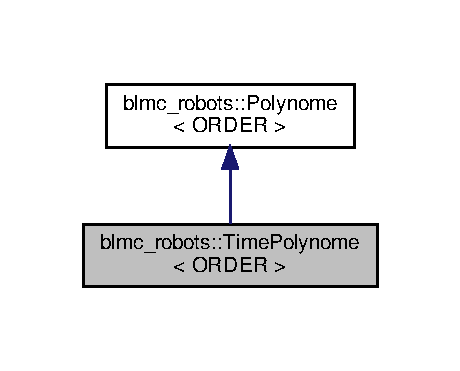
\includegraphics[width=221pt]{classblmc__robots_1_1TimePolynome__inherit__graph}
\end{center}
\end{figure}


Collaboration diagram for blmc\+\_\+robots\+:\+:Time\+Polynome$<$ O\+R\+D\+ER $>$\+:
\nopagebreak
\begin{figure}[H]
\begin{center}
\leavevmode
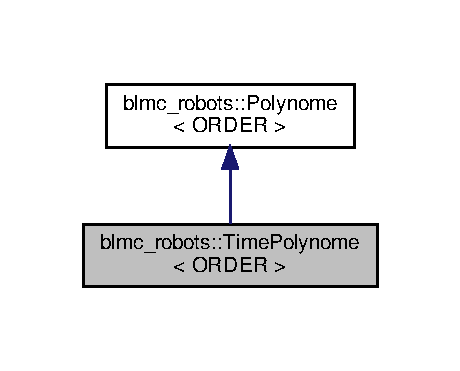
\includegraphics[width=221pt]{classblmc__robots_1_1TimePolynome__coll__graph}
\end{center}
\end{figure}
\subsection*{Public Member Functions}
\begin{DoxyCompactItemize}
\item 
\hyperlink{classblmc__robots_1_1TimePolynome_a0855aaf796c9d67302a5f2225355d745}{Time\+Polynome} ()
\item 
\hyperlink{classblmc__robots_1_1TimePolynome_add49c99d57206a93c9217f374f51700a}{$\sim$\+Time\+Polynome} ()
\item 
double \hyperlink{classblmc__robots_1_1TimePolynome_a644871336a78055c4e27e9b52e75ad8c}{compute} (double t)
\begin{DoxyCompactList}\small\item\em Time\+Polynome$<$\+O\+R\+D\+E\+R$>$ definitions. \end{DoxyCompactList}\item 
double \hyperlink{classblmc__robots_1_1TimePolynome_a089cd5e46da974828cfb1b042119c163}{compute\+\_\+derivative} (double t)
\item 
double \hyperlink{classblmc__robots_1_1TimePolynome_a3402f5a2e56b7ef46d93342f8c208bd1}{compute\+\_\+sec\+\_\+derivative} (double t)
\item 
\mbox{\Hypertarget{classblmc__robots_1_1TimePolynome_a8c6c6e522a9f4295c5d062afeb6f92a7}\label{classblmc__robots_1_1TimePolynome_a8c6c6e522a9f4295c5d062afeb6f92a7}} 
double {\bfseries get\+\_\+final\+\_\+time} () const
\item 
\mbox{\Hypertarget{classblmc__robots_1_1TimePolynome_a5700fc8407810b0be3a83149ead2516f}\label{classblmc__robots_1_1TimePolynome_a5700fc8407810b0be3a83149ead2516f}} 
double {\bfseries get\+\_\+init\+\_\+pose} () const
\item 
\mbox{\Hypertarget{classblmc__robots_1_1TimePolynome_acd83b243253bfb3eaa389b7162f04907}\label{classblmc__robots_1_1TimePolynome_acd83b243253bfb3eaa389b7162f04907}} 
double {\bfseries get\+\_\+init\+\_\+speed} () const
\item 
\mbox{\Hypertarget{classblmc__robots_1_1TimePolynome_aa88b45a138ac430a33ecd44fda40a94f}\label{classblmc__robots_1_1TimePolynome_aa88b45a138ac430a33ecd44fda40a94f}} 
double {\bfseries get\+\_\+init\+\_\+acc} () const
\item 
\mbox{\Hypertarget{classblmc__robots_1_1TimePolynome_a05fa06c51b2ad269f5773b0242f2fed7}\label{classblmc__robots_1_1TimePolynome_a05fa06c51b2ad269f5773b0242f2fed7}} 
double {\bfseries get\+\_\+final\+\_\+pose} () const
\item 
\mbox{\Hypertarget{classblmc__robots_1_1TimePolynome_acfb927d4c52380114308ec694eede80a}\label{classblmc__robots_1_1TimePolynome_acfb927d4c52380114308ec694eede80a}} 
double {\bfseries get\+\_\+final\+\_\+speed} () const
\item 
\mbox{\Hypertarget{classblmc__robots_1_1TimePolynome_aafdcb054558d12a22c1084ad844226c9}\label{classblmc__robots_1_1TimePolynome_aafdcb054558d12a22c1084ad844226c9}} 
double {\bfseries get\+\_\+final\+\_\+acc} () const
\item 
void \hyperlink{classblmc__robots_1_1TimePolynome_ac7576e3ab26e11a183268dcc4721e6e5}{set\+\_\+parameters} (double final\+\_\+time, double init\+\_\+pose, double init\+\_\+speed, double final\+\_\+pose)
\begin{DoxyCompactList}\small\item\em Computes a polynome trajectory according to the following constraints\+: \begin{eqnarray*} P(0) &=& init_pose \\ P(0) &=& init_speed = 0 \\ P(0) &=& init_acc = 0 \\ P(final_time_) &=& final_pose \\ P(final_time_) &=& final_speed = 0 \\ P(final_time_) &=& final_acc = 0 \end{eqnarray*}. \end{DoxyCompactList}\item 
\mbox{\Hypertarget{classblmc__robots_1_1TimePolynome_a46a01352c9e81a8135530facbf7cbcc6}\label{classblmc__robots_1_1TimePolynome_a46a01352c9e81a8135530facbf7cbcc6}} 
{\footnotesize template$<$$>$ }\\void {\bfseries set\+\_\+parameters} (double final\+\_\+time, double init\+\_\+pose, double init\+\_\+speed, double final\+\_\+pose)
\end{DoxyCompactItemize}
\subsection*{Protected Attributes}
\begin{DoxyCompactItemize}
\item 
\mbox{\Hypertarget{classblmc__robots_1_1TimePolynome_a08a973ac1a92ce4ae8b6053bea0b450e}\label{classblmc__robots_1_1TimePolynome_a08a973ac1a92ce4ae8b6053bea0b450e}} 
double \hyperlink{classblmc__robots_1_1TimePolynome_a08a973ac1a92ce4ae8b6053bea0b450e}{final\+\_\+time\+\_\+}
\begin{DoxyCompactList}\small\item\em store the inputs for later access \end{DoxyCompactList}\item 
\mbox{\Hypertarget{classblmc__robots_1_1TimePolynome_aaf83437483314782e67b4e6e23d8a222}\label{classblmc__robots_1_1TimePolynome_aaf83437483314782e67b4e6e23d8a222}} 
double \hyperlink{classblmc__robots_1_1TimePolynome_aaf83437483314782e67b4e6e23d8a222}{init\+\_\+pose\+\_\+}
\begin{DoxyCompactList}\small\item\em store the inputs for later access \end{DoxyCompactList}\item 
\mbox{\Hypertarget{classblmc__robots_1_1TimePolynome_a8a1387a89013f8d959e2eaaf4fb7048e}\label{classblmc__robots_1_1TimePolynome_a8a1387a89013f8d959e2eaaf4fb7048e}} 
double \hyperlink{classblmc__robots_1_1TimePolynome_a8a1387a89013f8d959e2eaaf4fb7048e}{init\+\_\+speed\+\_\+}
\begin{DoxyCompactList}\small\item\em store the inputs for later access \end{DoxyCompactList}\item 
\mbox{\Hypertarget{classblmc__robots_1_1TimePolynome_a9ecbcd9581dde19d9a86cd833d64349c}\label{classblmc__robots_1_1TimePolynome_a9ecbcd9581dde19d9a86cd833d64349c}} 
double \hyperlink{classblmc__robots_1_1TimePolynome_a9ecbcd9581dde19d9a86cd833d64349c}{init\+\_\+acc\+\_\+}
\begin{DoxyCompactList}\small\item\em store the inputs for later access \end{DoxyCompactList}\item 
\mbox{\Hypertarget{classblmc__robots_1_1TimePolynome_a427d2e970b5944d0f4cd6170aca99cc5}\label{classblmc__robots_1_1TimePolynome_a427d2e970b5944d0f4cd6170aca99cc5}} 
double \hyperlink{classblmc__robots_1_1TimePolynome_a427d2e970b5944d0f4cd6170aca99cc5}{final\+\_\+pose\+\_\+}
\begin{DoxyCompactList}\small\item\em store the inputs for later access \end{DoxyCompactList}\item 
\mbox{\Hypertarget{classblmc__robots_1_1TimePolynome_ac20c24571ce32d08834bc4d0530ed5e3}\label{classblmc__robots_1_1TimePolynome_ac20c24571ce32d08834bc4d0530ed5e3}} 
double \hyperlink{classblmc__robots_1_1TimePolynome_ac20c24571ce32d08834bc4d0530ed5e3}{final\+\_\+speed\+\_\+}
\begin{DoxyCompactList}\small\item\em store the inputs for later access \end{DoxyCompactList}\item 
\mbox{\Hypertarget{classblmc__robots_1_1TimePolynome_acdd91502f4a2e71f70539d1087347067}\label{classblmc__robots_1_1TimePolynome_acdd91502f4a2e71f70539d1087347067}} 
double \hyperlink{classblmc__robots_1_1TimePolynome_acdd91502f4a2e71f70539d1087347067}{final\+\_\+acc\+\_\+}
\begin{DoxyCompactList}\small\item\em store the inputs for later access \end{DoxyCompactList}\end{DoxyCompactItemize}


\subsection{Detailed Description}
\subsubsection*{template$<$int O\+R\+D\+ER$>$\newline
class blmc\+\_\+robots\+::\+Time\+Polynome$<$ O\+R\+D\+E\+R $>$}

Simple class that defines $ P(t) $ a polynome of order O\+R\+D\+ER. 

With $ t $ being the time in any units. It provide simple methods to compute safely $ P(time) $, $ \frac{dP}{dt}(t) $, and $ \frac{dP^2}{dt^2}(t) $


\begin{DoxyTemplParams}{Template Parameters}
{\em O\+R\+D\+ER} & \\
\hline
\end{DoxyTemplParams}


\subsection{Constructor \& Destructor Documentation}
\mbox{\Hypertarget{classblmc__robots_1_1TimePolynome_a0855aaf796c9d67302a5f2225355d745}\label{classblmc__robots_1_1TimePolynome_a0855aaf796c9d67302a5f2225355d745}} 
\index{blmc\+\_\+robots\+::\+Time\+Polynome@{blmc\+\_\+robots\+::\+Time\+Polynome}!Time\+Polynome@{Time\+Polynome}}
\index{Time\+Polynome@{Time\+Polynome}!blmc\+\_\+robots\+::\+Time\+Polynome@{blmc\+\_\+robots\+::\+Time\+Polynome}}
\subsubsection{\texorpdfstring{Time\+Polynome()}{TimePolynome()}}
{\footnotesize\ttfamily template$<$int O\+R\+D\+ER$>$ \\
\hyperlink{classblmc__robots_1_1TimePolynome}{blmc\+\_\+robots\+::\+Time\+Polynome}$<$ O\+R\+D\+ER $>$\+::\hyperlink{classblmc__robots_1_1TimePolynome}{Time\+Polynome} (\begin{DoxyParamCaption}{ }\end{DoxyParamCaption})\hspace{0.3cm}{\ttfamily [inline]}}

Constructor \mbox{\Hypertarget{classblmc__robots_1_1TimePolynome_add49c99d57206a93c9217f374f51700a}\label{classblmc__robots_1_1TimePolynome_add49c99d57206a93c9217f374f51700a}} 
\index{blmc\+\_\+robots\+::\+Time\+Polynome@{blmc\+\_\+robots\+::\+Time\+Polynome}!````~Time\+Polynome@{$\sim$\+Time\+Polynome}}
\index{````~Time\+Polynome@{$\sim$\+Time\+Polynome}!blmc\+\_\+robots\+::\+Time\+Polynome@{blmc\+\_\+robots\+::\+Time\+Polynome}}
\subsubsection{\texorpdfstring{$\sim$\+Time\+Polynome()}{~TimePolynome()}}
{\footnotesize\ttfamily template$<$int O\+R\+D\+ER$>$ \\
\hyperlink{classblmc__robots_1_1TimePolynome}{blmc\+\_\+robots\+::\+Time\+Polynome}$<$ O\+R\+D\+ER $>$\+::$\sim$\hyperlink{classblmc__robots_1_1TimePolynome}{Time\+Polynome} (\begin{DoxyParamCaption}{ }\end{DoxyParamCaption})\hspace{0.3cm}{\ttfamily [inline]}}

Destructor 

\subsection{Member Function Documentation}
\mbox{\Hypertarget{classblmc__robots_1_1TimePolynome_a644871336a78055c4e27e9b52e75ad8c}\label{classblmc__robots_1_1TimePolynome_a644871336a78055c4e27e9b52e75ad8c}} 
\index{blmc\+\_\+robots\+::\+Time\+Polynome@{blmc\+\_\+robots\+::\+Time\+Polynome}!compute@{compute}}
\index{compute@{compute}!blmc\+\_\+robots\+::\+Time\+Polynome@{blmc\+\_\+robots\+::\+Time\+Polynome}}
\subsubsection{\texorpdfstring{compute()}{compute()}}
{\footnotesize\ttfamily template$<$int O\+R\+D\+ER$>$ \\
double \hyperlink{classblmc__robots_1_1TimePolynome}{blmc\+\_\+robots\+::\+Time\+Polynome}$<$ O\+R\+D\+ER $>$\+::compute (\begin{DoxyParamCaption}\item[{double}]{t }\end{DoxyParamCaption})}



Time\+Polynome$<$\+O\+R\+D\+E\+R$>$ definitions. 

Compute the value. \mbox{\Hypertarget{classblmc__robots_1_1TimePolynome_a089cd5e46da974828cfb1b042119c163}\label{classblmc__robots_1_1TimePolynome_a089cd5e46da974828cfb1b042119c163}} 
\index{blmc\+\_\+robots\+::\+Time\+Polynome@{blmc\+\_\+robots\+::\+Time\+Polynome}!compute\+\_\+derivative@{compute\+\_\+derivative}}
\index{compute\+\_\+derivative@{compute\+\_\+derivative}!blmc\+\_\+robots\+::\+Time\+Polynome@{blmc\+\_\+robots\+::\+Time\+Polynome}}
\subsubsection{\texorpdfstring{compute\+\_\+derivative()}{compute\_derivative()}}
{\footnotesize\ttfamily template$<$int O\+R\+D\+ER$>$ \\
double \hyperlink{classblmc__robots_1_1TimePolynome}{blmc\+\_\+robots\+::\+Time\+Polynome}$<$ O\+R\+D\+ER $>$\+::compute\+\_\+derivative (\begin{DoxyParamCaption}\item[{double}]{t }\end{DoxyParamCaption})}

Compute the value of the derivative. \mbox{\Hypertarget{classblmc__robots_1_1TimePolynome_a3402f5a2e56b7ef46d93342f8c208bd1}\label{classblmc__robots_1_1TimePolynome_a3402f5a2e56b7ef46d93342f8c208bd1}} 
\index{blmc\+\_\+robots\+::\+Time\+Polynome@{blmc\+\_\+robots\+::\+Time\+Polynome}!compute\+\_\+sec\+\_\+derivative@{compute\+\_\+sec\+\_\+derivative}}
\index{compute\+\_\+sec\+\_\+derivative@{compute\+\_\+sec\+\_\+derivative}!blmc\+\_\+robots\+::\+Time\+Polynome@{blmc\+\_\+robots\+::\+Time\+Polynome}}
\subsubsection{\texorpdfstring{compute\+\_\+sec\+\_\+derivative()}{compute\_sec\_derivative()}}
{\footnotesize\ttfamily template$<$int O\+R\+D\+ER$>$ \\
double \hyperlink{classblmc__robots_1_1TimePolynome}{blmc\+\_\+robots\+::\+Time\+Polynome}$<$ O\+R\+D\+ER $>$\+::compute\+\_\+sec\+\_\+derivative (\begin{DoxyParamCaption}\item[{double}]{t }\end{DoxyParamCaption})}

Compute the value of the second derivative. \mbox{\Hypertarget{classblmc__robots_1_1TimePolynome_ac7576e3ab26e11a183268dcc4721e6e5}\label{classblmc__robots_1_1TimePolynome_ac7576e3ab26e11a183268dcc4721e6e5}} 
\index{blmc\+\_\+robots\+::\+Time\+Polynome@{blmc\+\_\+robots\+::\+Time\+Polynome}!set\+\_\+parameters@{set\+\_\+parameters}}
\index{set\+\_\+parameters@{set\+\_\+parameters}!blmc\+\_\+robots\+::\+Time\+Polynome@{blmc\+\_\+robots\+::\+Time\+Polynome}}
\subsubsection{\texorpdfstring{set\+\_\+parameters()}{set\_parameters()}}
{\footnotesize\ttfamily template$<$int O\+R\+D\+ER$>$ \\
void \hyperlink{classblmc__robots_1_1TimePolynome}{blmc\+\_\+robots\+::\+Time\+Polynome}$<$ O\+R\+D\+ER $>$\+::set\+\_\+parameters (\begin{DoxyParamCaption}\item[{double}]{final\+\_\+time,  }\item[{double}]{init\+\_\+pose,  }\item[{double}]{init\+\_\+speed,  }\item[{double}]{final\+\_\+pose }\end{DoxyParamCaption})}



Computes a polynome trajectory according to the following constraints\+: \begin{eqnarray*} P(0) &=& init_pose \\ P(0) &=& init_speed = 0 \\ P(0) &=& init_acc = 0 \\ P(final_time_) &=& final_pose \\ P(final_time_) &=& final_speed = 0 \\ P(final_time_) &=& final_acc = 0 \end{eqnarray*}. 


\begin{DoxyParams}{Parameters}
{\em final\+\_\+time} & is used in the constraints. \\
\hline
{\em init\+\_\+pose} & is used in the constraints. \\
\hline
{\em init\+\_\+speed} & is used in the constraints. \\
\hline
{\em final\+\_\+pose} & is used in the constraints. \\
\hline
\end{DoxyParams}


The documentation for this class was generated from the following files\+:\begin{DoxyCompactItemize}
\item 
include/blmc\+\_\+robots/mathematics/\hyperlink{polynome_8hpp}{polynome.\+hpp}\item 
include/blmc\+\_\+robots/mathematics/polynome.\+hxx\end{DoxyCompactItemize}

\hypertarget{structblmc__robots_1_1NJointBlmcRobotDriver_1_1Config_1_1TrajectoryStep}{}\section{blmc\+\_\+robots\+:\+:N\+Joint\+Blmc\+Robot\+Driver$<$ Observation, N\+\_\+\+J\+O\+I\+N\+TS, N\+\_\+\+M\+O\+T\+O\+R\+\_\+\+B\+O\+A\+R\+DS $>$\+:\+:Config\+:\+:Trajectory\+Step Struct Reference}
\label{structblmc__robots_1_1NJointBlmcRobotDriver_1_1Config_1_1TrajectoryStep}\index{blmc\+\_\+robots\+::\+N\+Joint\+Blmc\+Robot\+Driver$<$ Observation, N\+\_\+\+J\+O\+I\+N\+T\+S, N\+\_\+\+M\+O\+T\+O\+R\+\_\+\+B\+O\+A\+R\+D\+S $>$\+::\+Config\+::\+Trajectory\+Step@{blmc\+\_\+robots\+::\+N\+Joint\+Blmc\+Robot\+Driver$<$ Observation, N\+\_\+\+J\+O\+I\+N\+T\+S, N\+\_\+\+M\+O\+T\+O\+R\+\_\+\+B\+O\+A\+R\+D\+S $>$\+::\+Config\+::\+Trajectory\+Step}}


A sub-\/goal of a trajectory.  




{\ttfamily \#include $<$n\+\_\+joint\+\_\+blmc\+\_\+robot\+\_\+driver.\+hpp$>$}

\subsection*{Public Attributes}
\begin{DoxyCompactItemize}
\item 
\mbox{\Hypertarget{structblmc__robots_1_1NJointBlmcRobotDriver_1_1Config_1_1TrajectoryStep_a3c03278743cdf69bf8703b8aa79fcfa8}\label{structblmc__robots_1_1NJointBlmcRobotDriver_1_1Config_1_1TrajectoryStep_a3c03278743cdf69bf8703b8aa79fcfa8}} 
Vector \hyperlink{structblmc__robots_1_1NJointBlmcRobotDriver_1_1Config_1_1TrajectoryStep_a3c03278743cdf69bf8703b8aa79fcfa8}{target\+\_\+position\+\_\+rad} = Vector\+::\+Zero()
\begin{DoxyCompactList}\small\item\em Target position to which the joints should move. \end{DoxyCompactList}\item 
\mbox{\Hypertarget{structblmc__robots_1_1NJointBlmcRobotDriver_1_1Config_1_1TrajectoryStep_a7f25136ce7f8bfdbb2e049adee6d9312}\label{structblmc__robots_1_1NJointBlmcRobotDriver_1_1Config_1_1TrajectoryStep_a7f25136ce7f8bfdbb2e049adee6d9312}} 
uint32\+\_\+t \hyperlink{structblmc__robots_1_1NJointBlmcRobotDriver_1_1Config_1_1TrajectoryStep_a7f25136ce7f8bfdbb2e049adee6d9312}{move\+\_\+steps} = 0
\begin{DoxyCompactList}\small\item\em Number of time steps for reaching the target position. \end{DoxyCompactList}\end{DoxyCompactItemize}


\subsection{Detailed Description}
\subsubsection*{template$<$typename Observation, size\+\_\+t N\+\_\+\+J\+O\+I\+N\+TS, size\+\_\+t N\+\_\+\+M\+O\+T\+O\+R\+\_\+\+B\+O\+A\+R\+DS$>$\newline
struct blmc\+\_\+robots\+::\+N\+Joint\+Blmc\+Robot\+Driver$<$ Observation, N\+\_\+\+J\+O\+I\+N\+T\+S, N\+\_\+\+M\+O\+T\+O\+R\+\_\+\+B\+O\+A\+R\+D\+S $>$\+::\+Config\+::\+Trajectory\+Step}

A sub-\/goal of a trajectory. 

The documentation for this struct was generated from the following file\+:\begin{DoxyCompactItemize}
\item 
include/blmc\+\_\+robots/\hyperlink{n__joint__blmc__robot__driver_8hpp}{n\+\_\+joint\+\_\+blmc\+\_\+robot\+\_\+driver.\+hpp}\end{DoxyCompactItemize}

\chapter{File Documentation}
\hypertarget{common__demo__header_8hpp}{}\section{demos/common\+\_\+demo\+\_\+header.hpp File Reference}
\label{common__demo__header_8hpp}\index{demos/common\+\_\+demo\+\_\+header.\+hpp@{demos/common\+\_\+demo\+\_\+header.\+hpp}}


Contains some default tools for creating demos.  


{\ttfamily \#include \char`\"{}blmc\+\_\+robots/common\+\_\+programs\+\_\+header.\+hpp\char`\"{}}\newline
Include dependency graph for common\+\_\+demo\+\_\+header.\+hpp\+:
\nopagebreak
\begin{figure}[H]
\begin{center}
\leavevmode
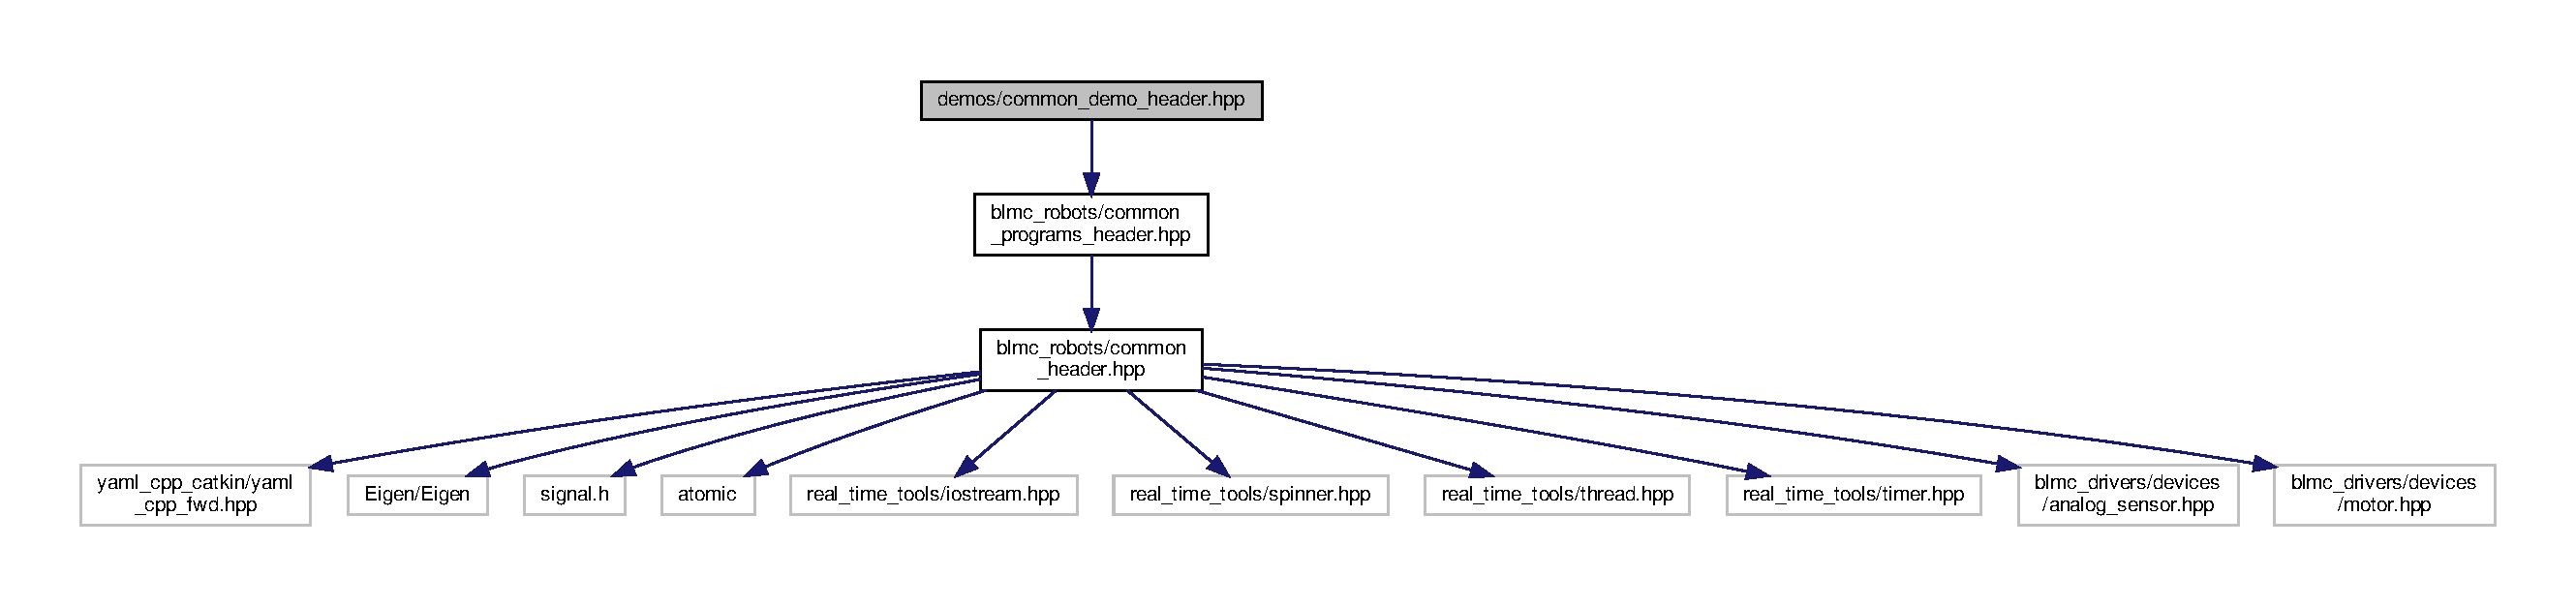
\includegraphics[width=350pt]{common__demo__header_8hpp__incl}
\end{center}
\end{figure}
This graph shows which files directly or indirectly include this file\+:
\nopagebreak
\begin{figure}[H]
\begin{center}
\leavevmode
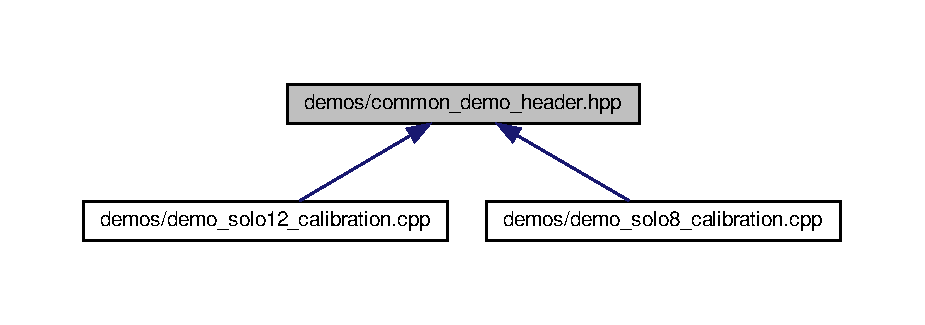
\includegraphics[width=350pt]{common__demo__header_8hpp__dep__incl}
\end{center}
\end{figure}
\subsection*{Classes}
\begin{DoxyCompactItemize}
\item 
struct \hyperlink{structblmc__robots_1_1ThreadCalibrationData}{blmc\+\_\+robots\+::\+Thread\+Calibration\+Data$<$ R\+O\+B\+O\+T\+\_\+\+T\+Y\+P\+E $>$}
\begin{DoxyCompactList}\small\item\em This small structure is used for reading the calibration parameters for the calibrations demos. \end{DoxyCompactList}\end{DoxyCompactItemize}


\subsection{Detailed Description}
Contains some default tools for creating demos. 

\begin{DoxyAuthor}{Author}
Maximilien Naveau (\href{mailto:maximilien.naveau@gmail.com}{\tt maximilien.\+naveau@gmail.\+com}) 
\end{DoxyAuthor}
\begin{DoxyVersion}{Version}
0.\+1 
\end{DoxyVersion}
\begin{DoxyDate}{Date}
2019-\/11-\/07
\end{DoxyDate}
\begin{DoxyCopyright}{Copyright}
Copyright (c) 2019 
\end{DoxyCopyright}

\hypertarget{demo__solo12_8cpp}{}\section{demos/demo\+\_\+solo12.cpp File Reference}
\label{demo__solo12_8cpp}\index{demos/demo\+\_\+solo12.\+cpp@{demos/demo\+\_\+solo12.\+cpp}}


Implements basic PD controller reading slider values.  


{\ttfamily \#include $<$numeric$>$}\newline
{\ttfamily \#include \char`\"{}blmc\+\_\+robots/common\+\_\+programs\+\_\+header.\+hpp\char`\"{}}\newline
{\ttfamily \#include \char`\"{}blmc\+\_\+robots/solo12.\+hpp\char`\"{}}\newline
Include dependency graph for demo\+\_\+solo12.\+cpp\+:
\nopagebreak
\begin{figure}[H]
\begin{center}
\leavevmode
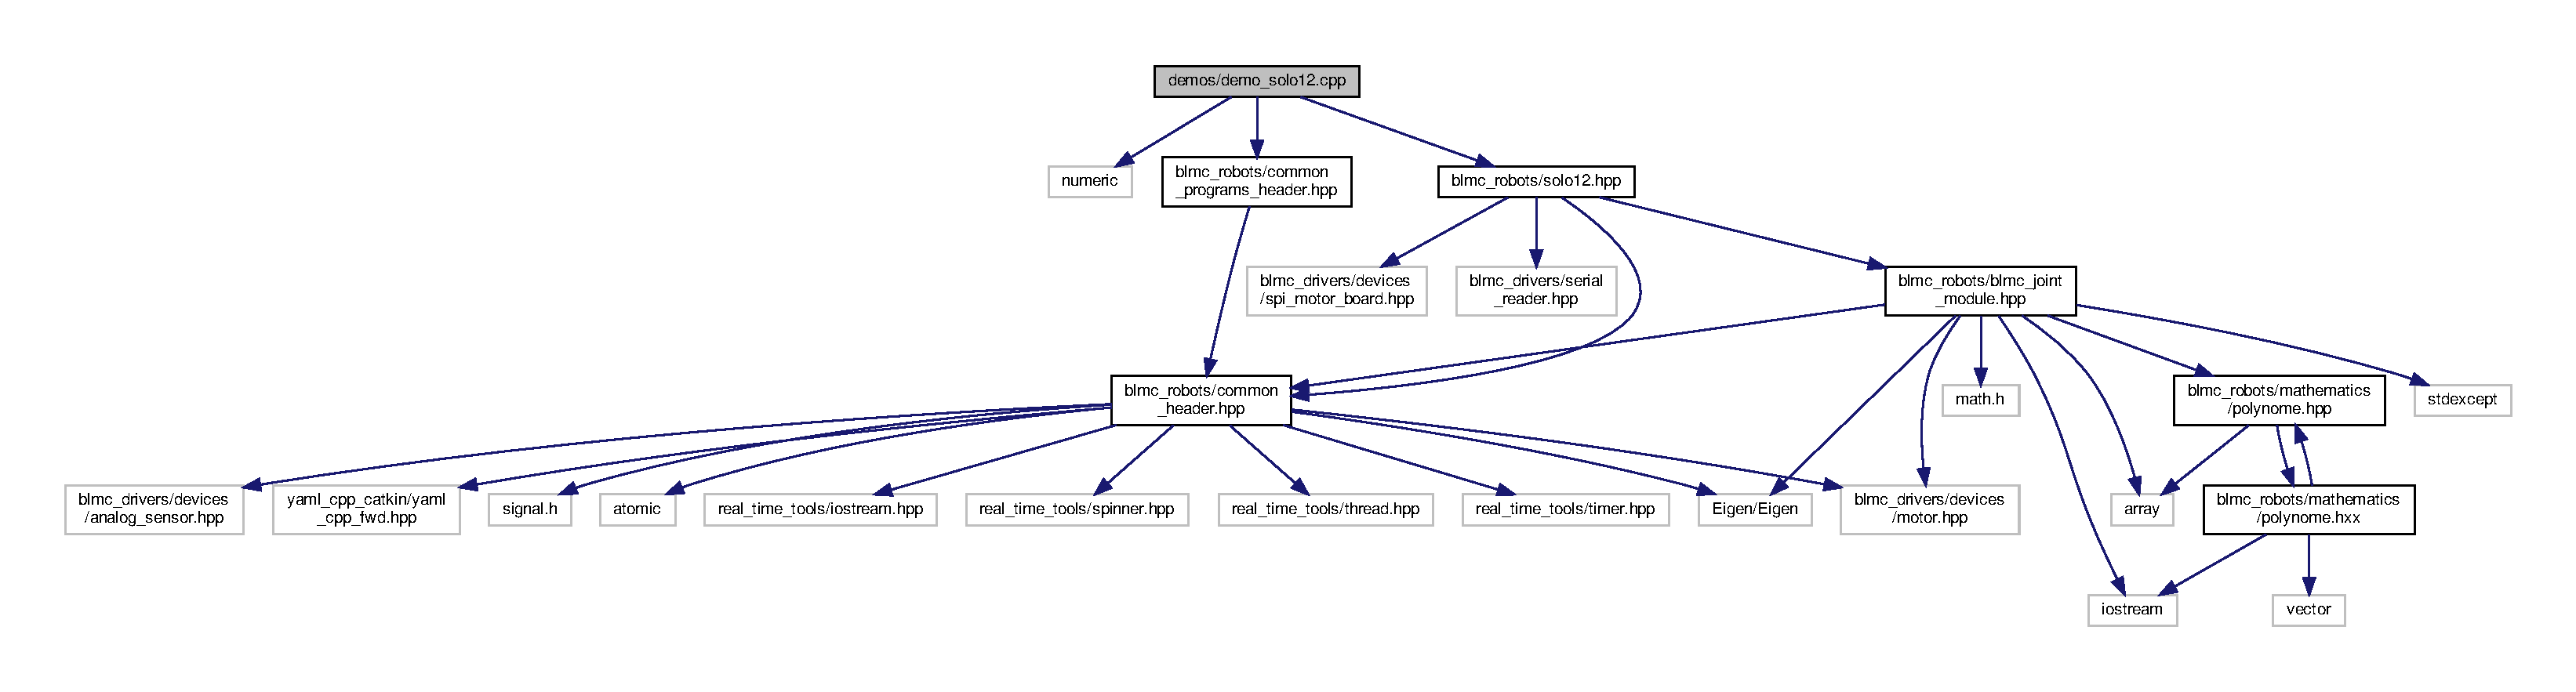
\includegraphics[width=350pt]{demo__solo12_8cpp__incl}
\end{center}
\end{figure}
\subsection*{Functions}
\begin{DoxyCompactItemize}
\item 
\mbox{\Hypertarget{demo__solo12_8cpp_a5b91a2c54c5572ad9e3a9c2d295263b3}\label{demo__solo12_8cpp_a5b91a2c54c5572ad9e3a9c2d295263b3}} 
void {\bfseries map\+\_\+sliders} (Eigen\+::\+Ref$<$ Eigen\+::\+Vector4d $>$ sliders, Eigen\+::\+Ref$<$ \hyperlink{common__header_8hpp_a80313eb420184518596e745eecf4b494}{Vector12d} $>$ sliders\+\_\+out)
\item 
\mbox{\Hypertarget{demo__solo12_8cpp_ad6c628b757f67738bfae2ffb51a453c1}\label{demo__solo12_8cpp_ad6c628b757f67738bfae2ffb51a453c1}} 
static T\+H\+R\+E\+A\+D\+\_\+\+F\+U\+N\+C\+T\+I\+O\+N\+\_\+\+R\+E\+T\+U\+R\+N\+\_\+\+T\+Y\+PE {\bfseries control\+\_\+loop} (void $\ast$args)
\item 
\mbox{\Hypertarget{demo__solo12_8cpp_a3c04138a5bfe5d72780bb7e82a18e627}\label{demo__solo12_8cpp_a3c04138a5bfe5d72780bb7e82a18e627}} 
int {\bfseries main} (int argc, char $\ast$$\ast$argv)
\end{DoxyCompactItemize}


\subsection{Detailed Description}
Implements basic PD controller reading slider values. 

\begin{DoxyAuthor}{Author}
Julian Viereck 
\end{DoxyAuthor}
\begin{DoxyDate}{Date}
21 November 2019
\end{DoxyDate}
This file uses the Solo12 class in a small demo. 
\hypertarget{demo__solo12__calibration_8cpp}{}\section{demos/demo\+\_\+solo12\+\_\+calibration.cpp File Reference}
\label{demo__solo12__calibration_8cpp}\index{demos/demo\+\_\+solo12\+\_\+calibration.\+cpp@{demos/demo\+\_\+solo12\+\_\+calibration.\+cpp}}


Small demo to test the calibration on the real robot.  


{\ttfamily \#include \char`\"{}blmc\+\_\+robots/solo12.\+hpp\char`\"{}}\newline
{\ttfamily \#include \char`\"{}common\+\_\+demo\+\_\+header.\+hpp\char`\"{}}\newline
Include dependency graph for demo\+\_\+solo12\+\_\+calibration.\+cpp\+:
\nopagebreak
\begin{figure}[H]
\begin{center}
\leavevmode
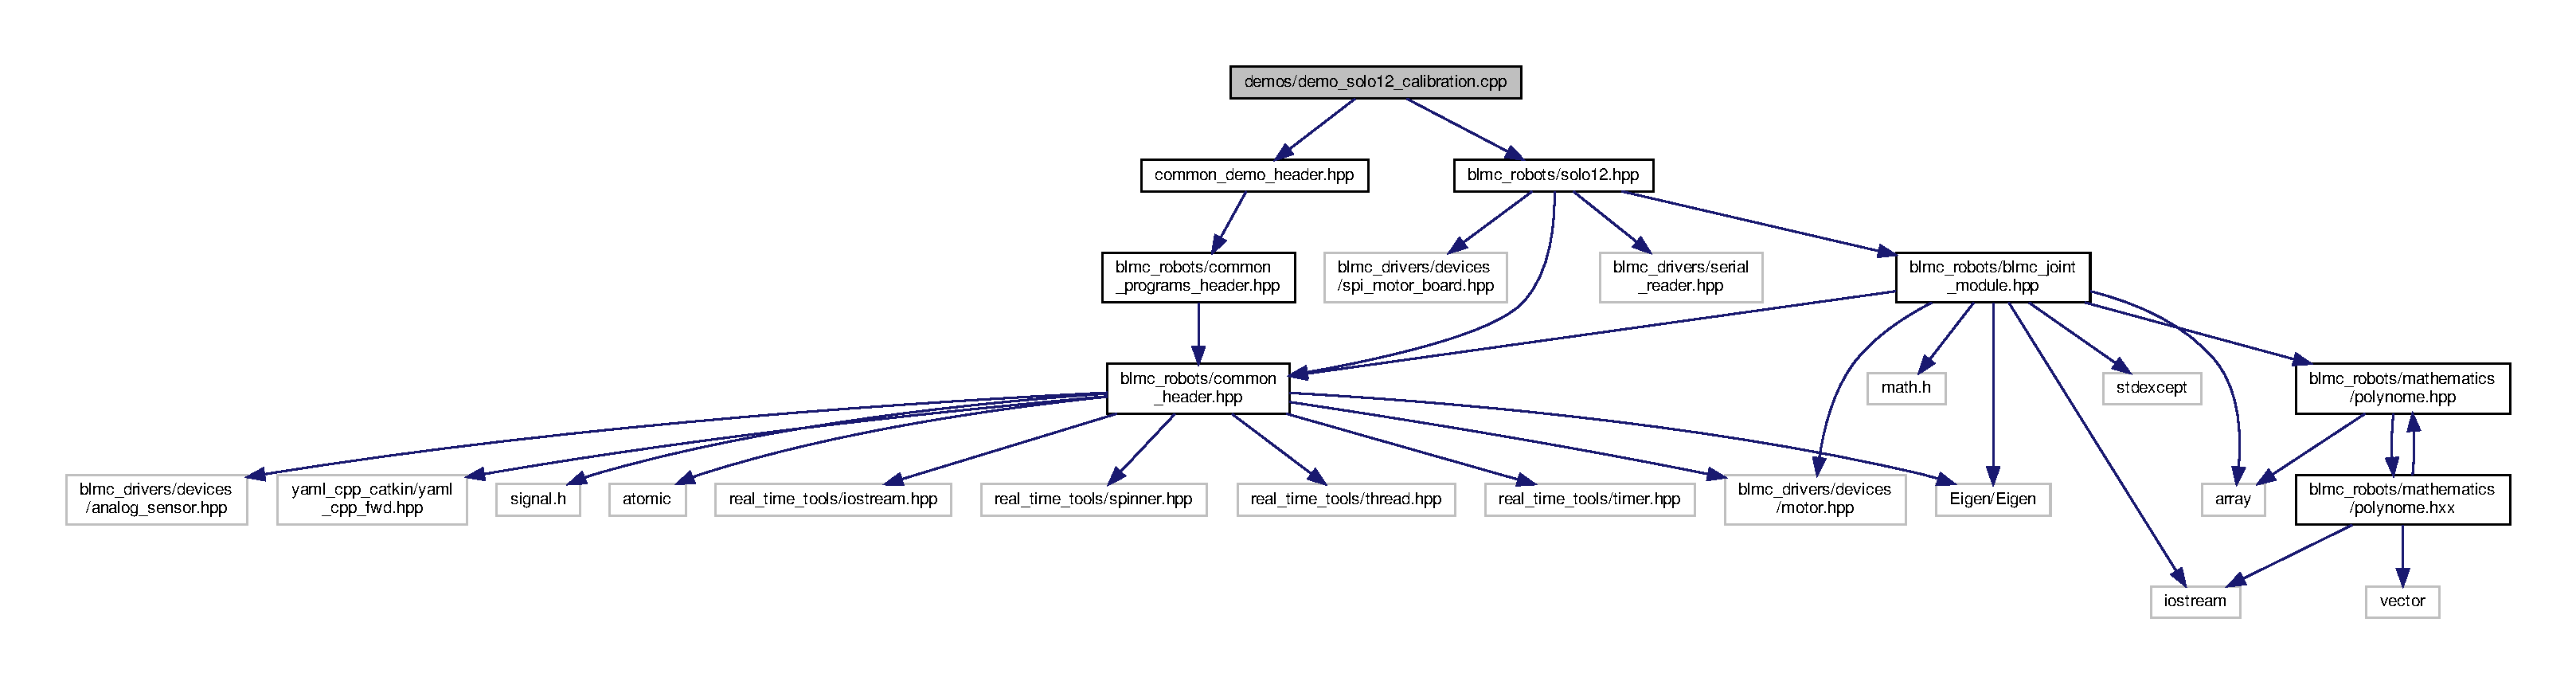
\includegraphics[width=350pt]{demo__solo12__calibration_8cpp__incl}
\end{center}
\end{figure}
\subsection*{Typedefs}
\begin{DoxyCompactItemize}
\item 
\mbox{\Hypertarget{demo__solo12__calibration_8cpp_ab9d429cb6b4af0823d111594c5792593}\label{demo__solo12__calibration_8cpp_ab9d429cb6b4af0823d111594c5792593}} 
typedef \hyperlink{structblmc__robots_1_1ThreadCalibrationData}{Thread\+Calibration\+Data}$<$ \hyperlink{classblmc__robots_1_1Solo12}{Solo12} $>$ {\bfseries Thread\+Calibration\+Data\+\_\+t}
\end{DoxyCompactItemize}
\subsection*{Functions}
\begin{DoxyCompactItemize}
\item 
\mbox{\Hypertarget{demo__solo12__calibration_8cpp_a4061cd7d86b33a32f45bdce36ac5dea2}\label{demo__solo12__calibration_8cpp_a4061cd7d86b33a32f45bdce36ac5dea2}} 
static T\+H\+R\+E\+A\+D\+\_\+\+F\+U\+N\+C\+T\+I\+O\+N\+\_\+\+R\+E\+T\+U\+R\+N\+\_\+\+T\+Y\+PE {\bfseries control\+\_\+loop} (void $\ast$thread\+\_\+data\+\_\+void\+\_\+ptr)
\item 
\mbox{\Hypertarget{demo__solo12__calibration_8cpp_a3c04138a5bfe5d72780bb7e82a18e627}\label{demo__solo12__calibration_8cpp_a3c04138a5bfe5d72780bb7e82a18e627}} 
int {\bfseries main} (int argc, char $\ast$$\ast$argv)
\end{DoxyCompactItemize}


\subsection{Detailed Description}
Small demo to test the calibration on the real robot. 

\begin{DoxyAuthor}{Author}
Maximilien Naveau (\href{mailto:maximilien.naveau@gmail.com}{\tt maximilien.\+naveau@gmail.\+com}) 
\end{DoxyAuthor}
\begin{DoxyVersion}{Version}
0.\+1 
\end{DoxyVersion}
\begin{DoxyDate}{Date}
2019-\/11-\/08
\end{DoxyDate}
\begin{DoxyCopyright}{Copyright}
Copyright (c) 2019 
\end{DoxyCopyright}

\hypertarget{demo__solo8_8cpp}{}\section{demos/demo\+\_\+solo8.cpp File Reference}
\label{demo__solo8_8cpp}\index{demos/demo\+\_\+solo8.\+cpp@{demos/demo\+\_\+solo8.\+cpp}}


The use of the wrapper implementing a small pid controller.  


{\ttfamily \#include $<$numeric$>$}\newline
{\ttfamily \#include \char`\"{}blmc\+\_\+robots/common\+\_\+programs\+\_\+header.\+hpp\char`\"{}}\newline
{\ttfamily \#include \char`\"{}blmc\+\_\+robots/solo8.\+hpp\char`\"{}}\newline
Include dependency graph for demo\+\_\+solo8.\+cpp\+:
\nopagebreak
\begin{figure}[H]
\begin{center}
\leavevmode
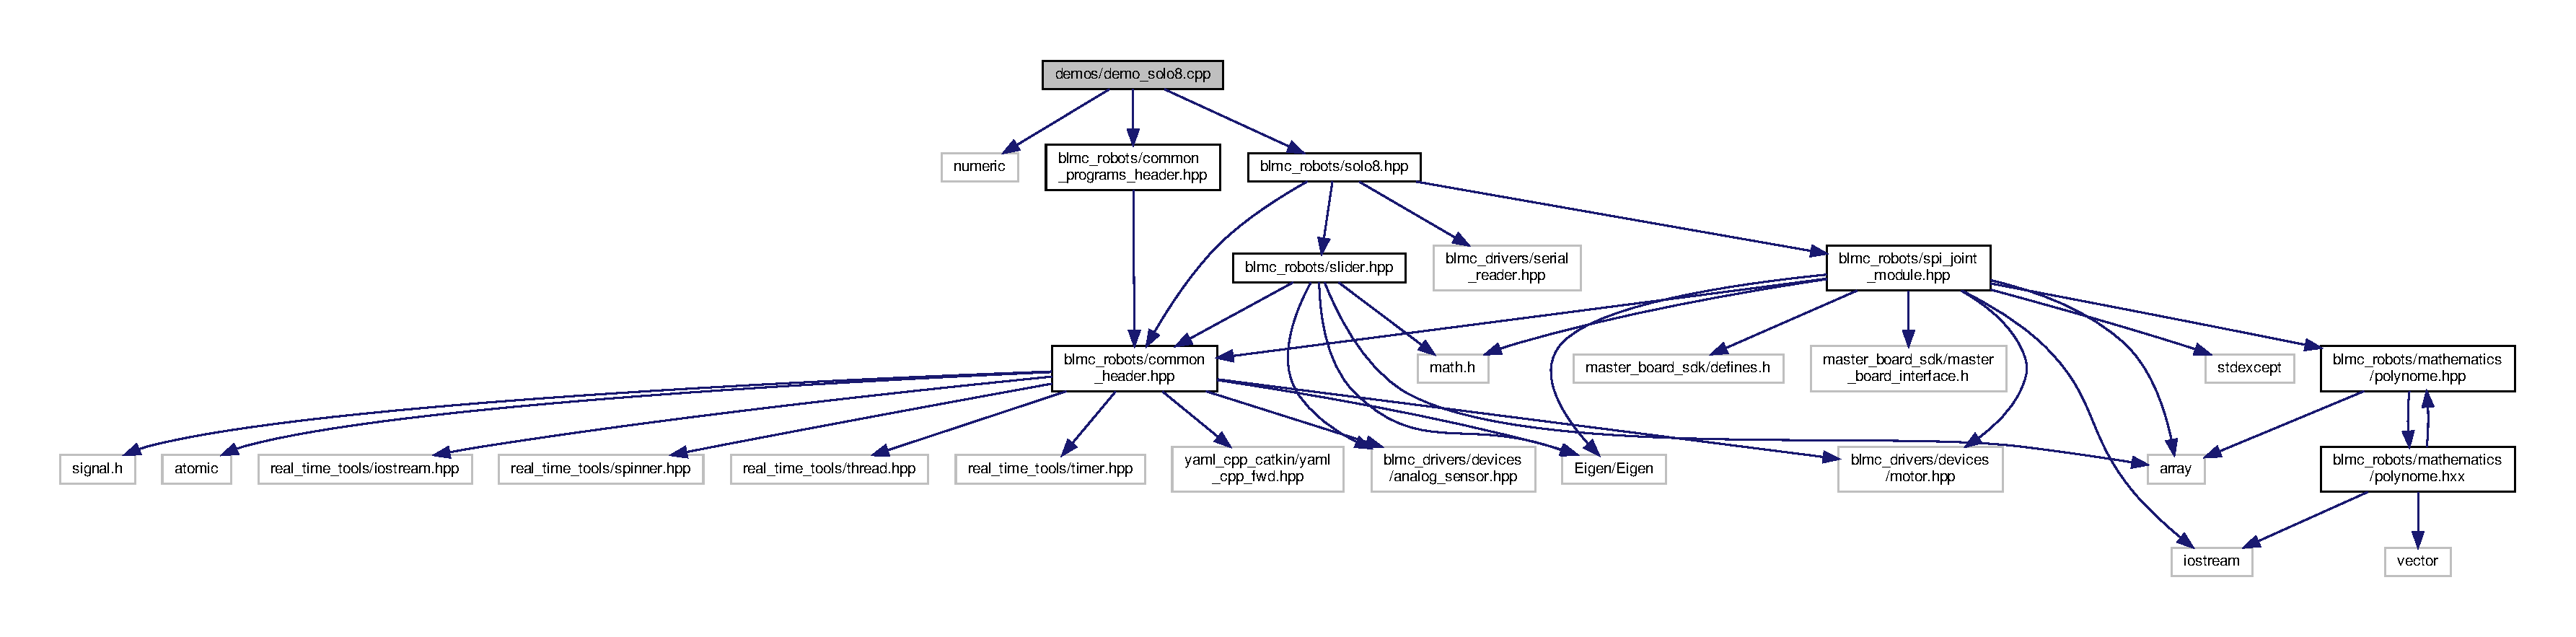
\includegraphics[width=350pt]{demo__solo8_8cpp__incl}
\end{center}
\end{figure}
\subsection*{Functions}
\begin{DoxyCompactItemize}
\item 
\mbox{\Hypertarget{demo__solo8_8cpp_a39957cbbba118d0d10bbc093b6b1ff5a}\label{demo__solo8_8cpp_a39957cbbba118d0d10bbc093b6b1ff5a}} 
static T\+H\+R\+E\+A\+D\+\_\+\+F\+U\+N\+C\+T\+I\+O\+N\+\_\+\+R\+E\+T\+U\+R\+N\+\_\+\+T\+Y\+PE {\bfseries control\+\_\+loop} (void $\ast$robot\+\_\+void\+\_\+ptr)
\item 
\mbox{\Hypertarget{demo__solo8_8cpp_a3c04138a5bfe5d72780bb7e82a18e627}\label{demo__solo8_8cpp_a3c04138a5bfe5d72780bb7e82a18e627}} 
int {\bfseries main} (int argc, char $\ast$$\ast$argv)
\end{DoxyCompactItemize}


\subsection{Detailed Description}
The use of the wrapper implementing a small pid controller. 

\begin{DoxyAuthor}{Author}
Maximilien Naveau 
\end{DoxyAuthor}
\begin{DoxyDate}{Date}
2018
\end{DoxyDate}
This file uses the Solo8 class in a small demo. 
\hypertarget{demo__solo8__calibration_8cpp}{}\section{demos/demo\+\_\+solo8\+\_\+calibration.cpp File Reference}
\label{demo__solo8__calibration_8cpp}\index{demos/demo\+\_\+solo8\+\_\+calibration.\+cpp@{demos/demo\+\_\+solo8\+\_\+calibration.\+cpp}}


Small demo to test the calibration on the real robot.  


{\ttfamily \#include \char`\"{}blmc\+\_\+robots/solo8.\+hpp\char`\"{}}\newline
{\ttfamily \#include \char`\"{}common\+\_\+demo\+\_\+header.\+hpp\char`\"{}}\newline
Include dependency graph for demo\+\_\+solo8\+\_\+calibration.\+cpp\+:
\nopagebreak
\begin{figure}[H]
\begin{center}
\leavevmode
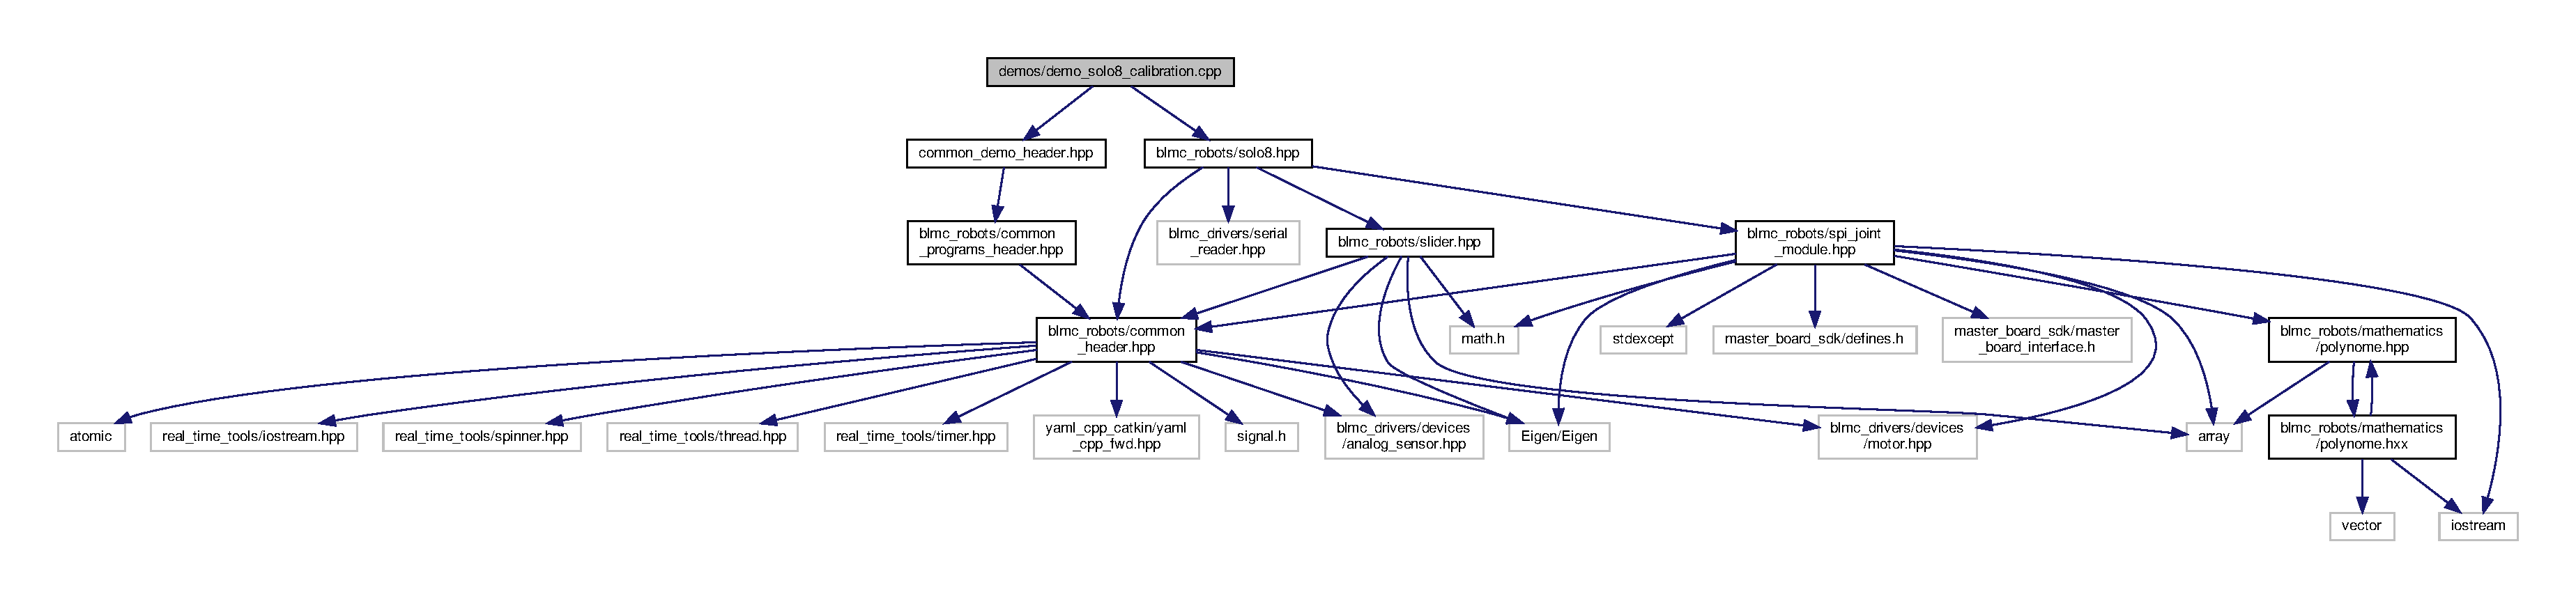
\includegraphics[width=350pt]{demo__solo8__calibration_8cpp__incl}
\end{center}
\end{figure}
\subsection*{Typedefs}
\begin{DoxyCompactItemize}
\item 
\mbox{\Hypertarget{demo__solo8__calibration_8cpp_acd044edbe93d182715a33f4db42fa297}\label{demo__solo8__calibration_8cpp_acd044edbe93d182715a33f4db42fa297}} 
typedef \hyperlink{structblmc__robots_1_1ThreadCalibrationData}{Thread\+Calibration\+Data}$<$ \hyperlink{classblmc__robots_1_1Solo8}{Solo8} $>$ {\bfseries Thread\+Calibration\+Data\+\_\+t}
\end{DoxyCompactItemize}
\subsection*{Functions}
\begin{DoxyCompactItemize}
\item 
\mbox{\Hypertarget{demo__solo8__calibration_8cpp_a4061cd7d86b33a32f45bdce36ac5dea2}\label{demo__solo8__calibration_8cpp_a4061cd7d86b33a32f45bdce36ac5dea2}} 
static T\+H\+R\+E\+A\+D\+\_\+\+F\+U\+N\+C\+T\+I\+O\+N\+\_\+\+R\+E\+T\+U\+R\+N\+\_\+\+T\+Y\+PE {\bfseries control\+\_\+loop} (void $\ast$thread\+\_\+data\+\_\+void\+\_\+ptr)
\item 
\mbox{\Hypertarget{demo__solo8__calibration_8cpp_a3c04138a5bfe5d72780bb7e82a18e627}\label{demo__solo8__calibration_8cpp_a3c04138a5bfe5d72780bb7e82a18e627}} 
int {\bfseries main} (int argc, char $\ast$$\ast$argv)
\end{DoxyCompactItemize}


\subsection{Detailed Description}
Small demo to test the calibration on the real robot. 

\begin{DoxyAuthor}{Author}
Maximilien Naveau (\href{mailto:maximilien.naveau@gmail.com}{\tt maximilien.\+naveau@gmail.\+com}) 
\end{DoxyAuthor}
\begin{DoxyVersion}{Version}
0.\+1 
\end{DoxyVersion}
\begin{DoxyDate}{Date}
2019-\/11-\/08
\end{DoxyDate}
\begin{DoxyCopyright}{Copyright}
Copyright (c) 2019 
\end{DoxyCopyright}

\hypertarget{demo__test__bench__8__motors_8cpp}{}\section{demos/demo\+\_\+test\+\_\+bench\+\_\+8\+\_\+motors.cpp File Reference}
\label{demo__test__bench__8__motors_8cpp}\index{demos/demo\+\_\+test\+\_\+bench\+\_\+8\+\_\+motors.\+cpp@{demos/demo\+\_\+test\+\_\+bench\+\_\+8\+\_\+motors.\+cpp}}


The use of the wrapper implementing a small pid controller.  


{\ttfamily \#include \char`\"{}blmc\+\_\+robots/common\+\_\+programs\+\_\+header.\+hpp\char`\"{}}\newline
{\ttfamily \#include \char`\"{}blmc\+\_\+robots/test\+\_\+bench\+\_\+8\+\_\+motors.\+hpp\char`\"{}}\newline
Include dependency graph for demo\+\_\+test\+\_\+bench\+\_\+8\+\_\+motors.\+cpp\+:
\nopagebreak
\begin{figure}[H]
\begin{center}
\leavevmode
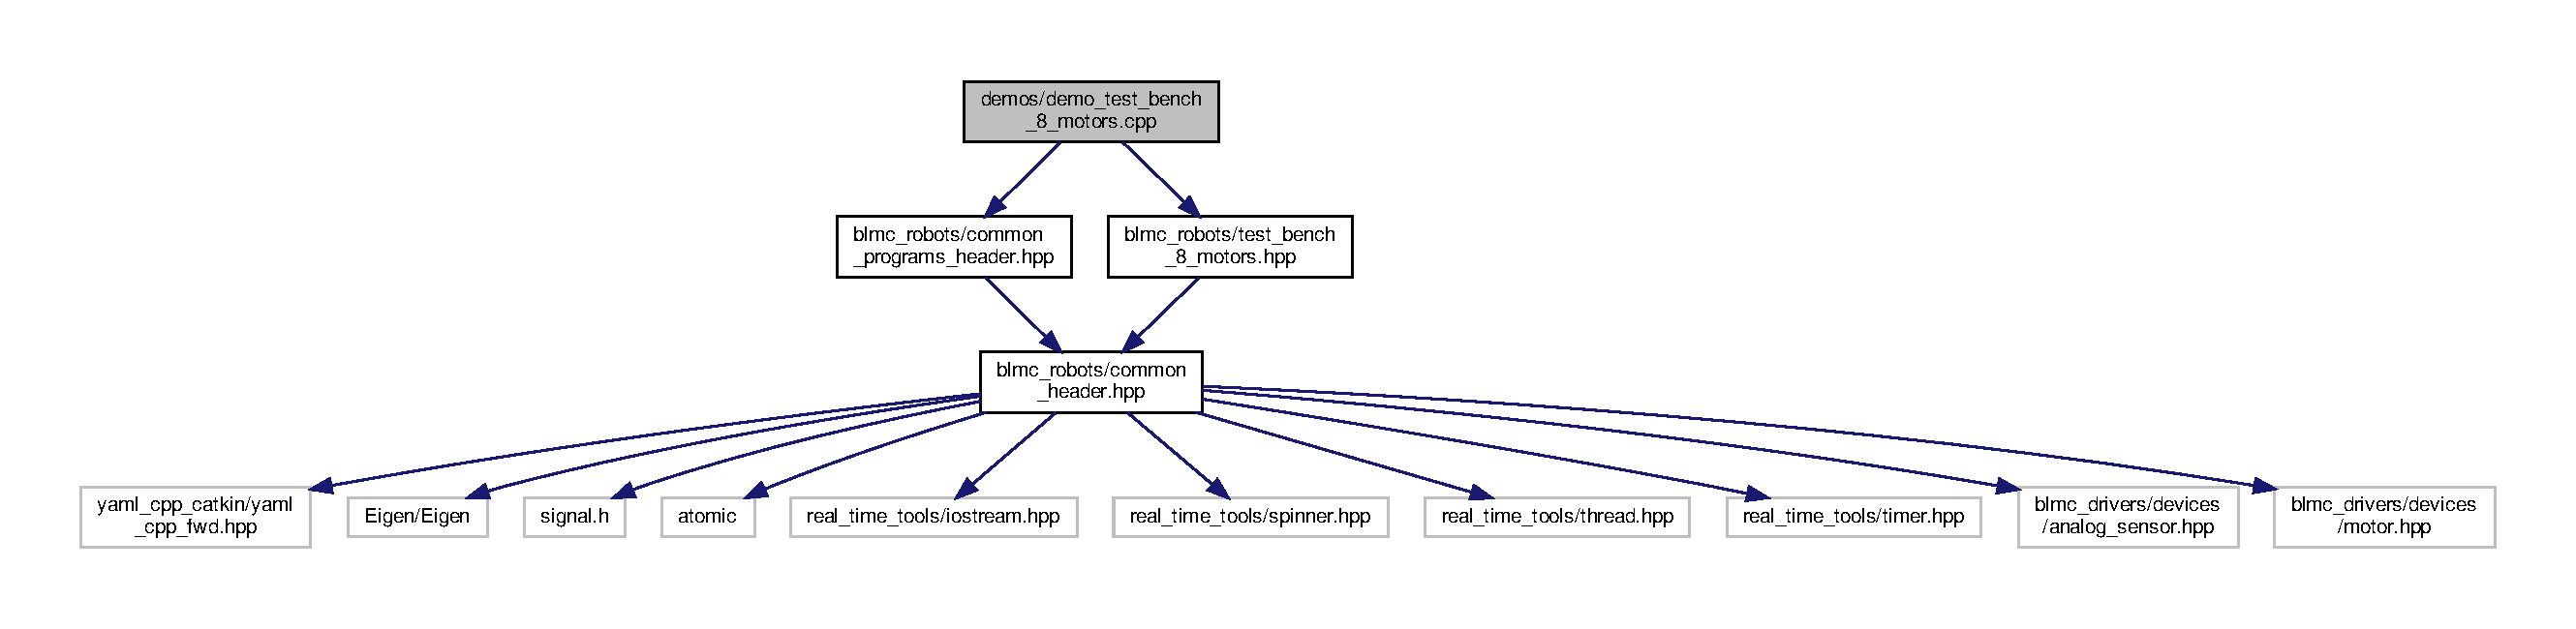
\includegraphics[width=350pt]{demo__test__bench__8__motors_8cpp__incl}
\end{center}
\end{figure}
\subsection*{Functions}
\begin{DoxyCompactItemize}
\item 
\mbox{\Hypertarget{demo__test__bench__8__motors_8cpp_a39957cbbba118d0d10bbc093b6b1ff5a}\label{demo__test__bench__8__motors_8cpp_a39957cbbba118d0d10bbc093b6b1ff5a}} 
static T\+H\+R\+E\+A\+D\+\_\+\+F\+U\+N\+C\+T\+I\+O\+N\+\_\+\+R\+E\+T\+U\+R\+N\+\_\+\+T\+Y\+PE {\bfseries control\+\_\+loop} (void $\ast$robot\+\_\+void\+\_\+ptr)
\item 
\mbox{\Hypertarget{demo__test__bench__8__motors_8cpp_a2c3f6775325c30275d11c6abee2db6a0}\label{demo__test__bench__8__motors_8cpp_a2c3f6775325c30275d11c6abee2db6a0}} 
int {\bfseries main} (int, char $\ast$$\ast$)
\end{DoxyCompactItemize}


\subsection{Detailed Description}
The use of the wrapper implementing a small pid controller. 

\begin{DoxyAuthor}{Author}
Maximilien Naveau 
\end{DoxyAuthor}
\begin{DoxyDate}{Date}
2018
\end{DoxyDate}
This file uses the Stuggihop class in a small demo.

\begin{DoxyAuthor}{Author}
Maximilien Naveau 
\end{DoxyAuthor}
\begin{DoxyDate}{Date}
2018
\end{DoxyDate}
This file uses the Test\+Bench8\+Motors class in a small demo.

\begin{DoxyAuthor}{Author}
Maximilien Naveau 
\end{DoxyAuthor}
\begin{DoxyDate}{Date}
2018
\end{DoxyDate}
This file uses the Teststand class in a small demo. 
\hypertarget{blmc__joint__module_8hpp}{}\section{include/blmc\+\_\+robots/blmc\+\_\+joint\+\_\+module.hpp File Reference}
\label{blmc__joint__module_8hpp}\index{include/blmc\+\_\+robots/blmc\+\_\+joint\+\_\+module.\+hpp@{include/blmc\+\_\+robots/blmc\+\_\+joint\+\_\+module.\+hpp}}
{\ttfamily \#include $<$math.\+h$>$}\newline
{\ttfamily \#include $<$Eigen/\+Eigen$>$}\newline
{\ttfamily \#include $<$array$>$}\newline
{\ttfamily \#include $<$iostream$>$}\newline
{\ttfamily \#include $<$stdexcept$>$}\newline
{\ttfamily \#include \char`\"{}blmc\+\_\+drivers/devices/motor.\+hpp\char`\"{}}\newline
{\ttfamily \#include \char`\"{}blmc\+\_\+robots/common\+\_\+header.\+hpp\char`\"{}}\newline
{\ttfamily \#include \char`\"{}blmc\+\_\+robots/mathematics/polynome.\+hpp\char`\"{}}\newline
Include dependency graph for blmc\+\_\+joint\+\_\+module.\+hpp\+:
\nopagebreak
\begin{figure}[H]
\begin{center}
\leavevmode
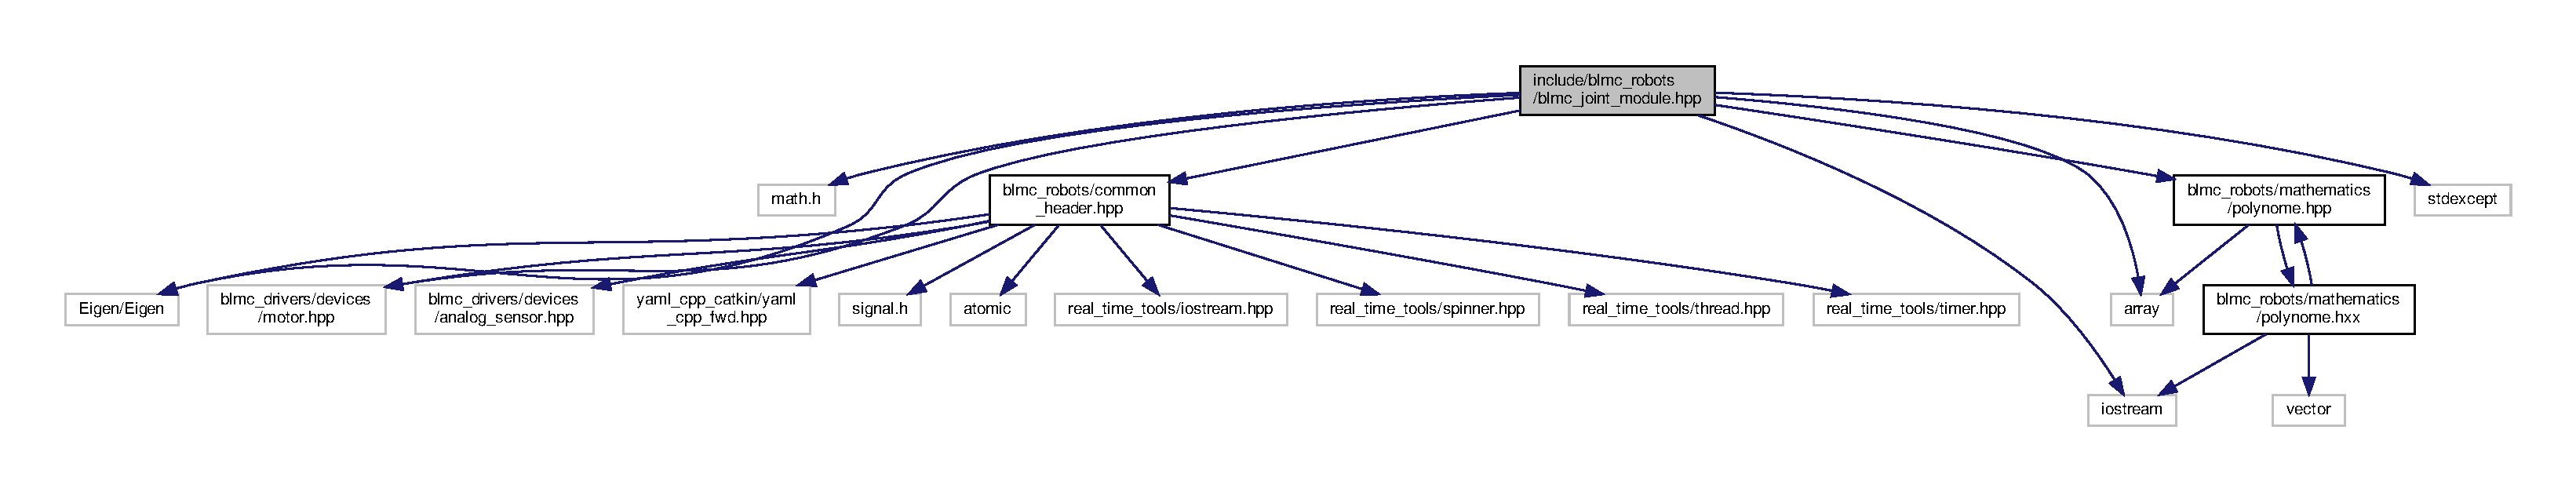
\includegraphics[width=350pt]{blmc__joint__module_8hpp__incl}
\end{center}
\end{figure}
This graph shows which files directly or indirectly include this file\+:
\nopagebreak
\begin{figure}[H]
\begin{center}
\leavevmode
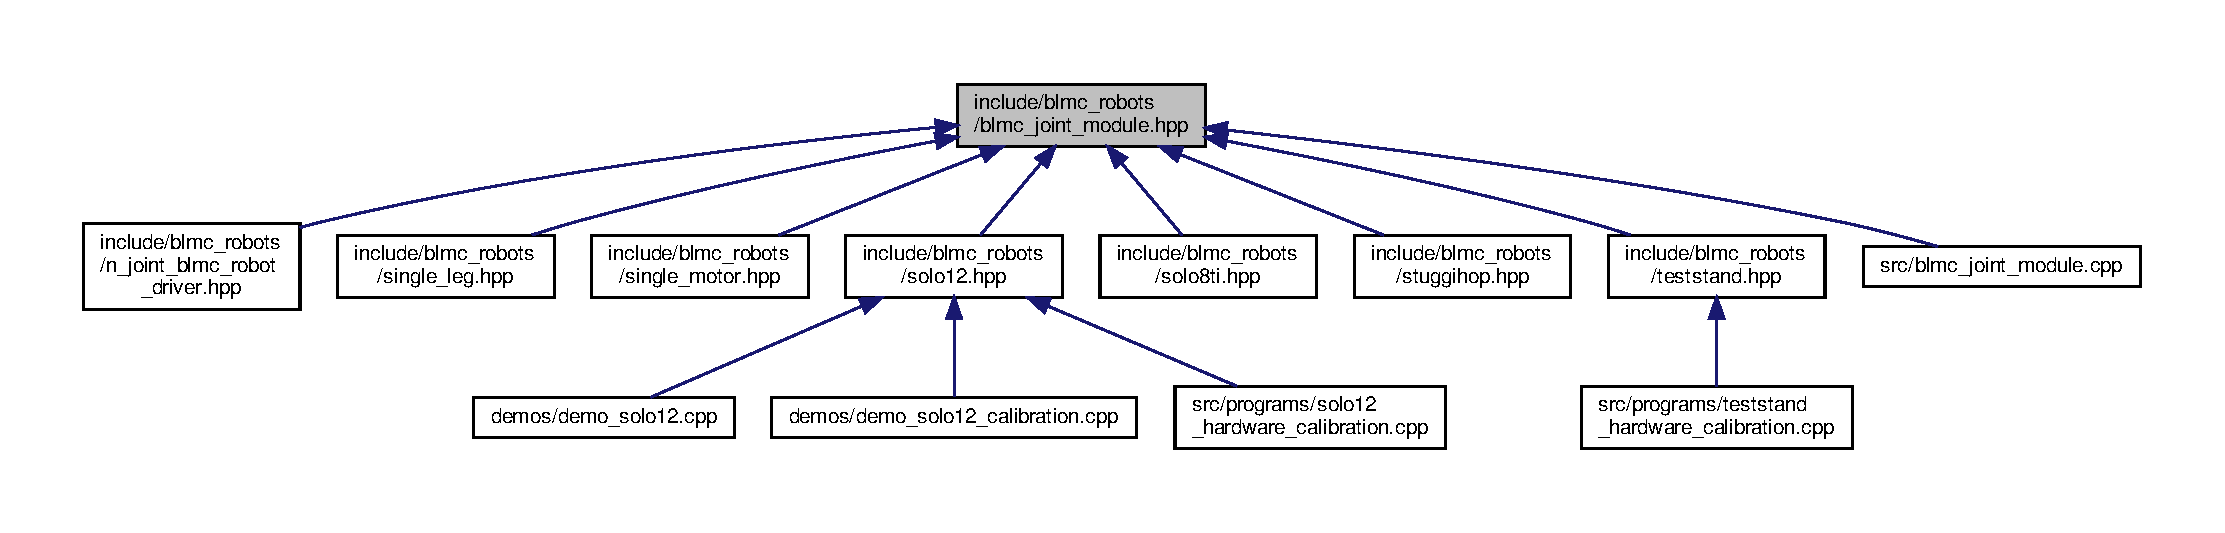
\includegraphics[width=350pt]{blmc__joint__module_8hpp__dep__incl}
\end{center}
\end{figure}
\subsection*{Classes}
\begin{DoxyCompactItemize}
\item 
struct \hyperlink{structblmc__robots_1_1HomingState}{blmc\+\_\+robots\+::\+Homing\+State}
\begin{DoxyCompactList}\small\item\em State variables required for the homing. \end{DoxyCompactList}\item 
class \hyperlink{classblmc__robots_1_1BlmcJointModule}{blmc\+\_\+robots\+::\+Blmc\+Joint\+Module}
\begin{DoxyCompactList}\small\item\em The \hyperlink{classblmc__robots_1_1BlmcJointModule}{Blmc\+Joint\+Module} class is containing the joint information. \end{DoxyCompactList}\item 
class \hyperlink{classblmc__robots_1_1BlmcJointModules}{blmc\+\_\+robots\+::\+Blmc\+Joint\+Modules$<$ C\+O\+U\+N\+T $>$}
\begin{DoxyCompactList}\small\item\em This class defines an interface to a collection of B\+L\+MC joints. \end{DoxyCompactList}\end{DoxyCompactItemize}
\subsection*{Typedefs}
\begin{DoxyCompactItemize}
\item 
\mbox{\Hypertarget{blmc__joint__module_8hpp_aa5066dce11e2e3ae56b844676b132a09}\label{blmc__joint__module_8hpp_aa5066dce11e2e3ae56b844676b132a09}} 
typedef std\+::shared\+\_\+ptr$<$ Blmc\+Joint\+Module $>$ \hyperlink{blmc__joint__module_8hpp_aa5066dce11e2e3ae56b844676b132a09}{blmc\+\_\+robots\+::\+Blmc\+Joint\+Module\+\_\+ptr}
\begin{DoxyCompactList}\small\item\em Blmc\+Joint\+Module\+\_\+ptr shortcut for the shared pointer \hyperlink{classblmc__robots_1_1BlmcJointModule}{Blmc\+Joint\+Module} type. \end{DoxyCompactList}\end{DoxyCompactItemize}
\subsection*{Enumerations}
\begin{DoxyCompactItemize}
\item 
\mbox{\Hypertarget{blmc__joint__module_8hpp_aa1075809042ff261e4b0a20d161448b6}\label{blmc__joint__module_8hpp_aa1075809042ff261e4b0a20d161448b6}} 
enum \hyperlink{blmc__joint__module_8hpp_aa1075809042ff261e4b0a20d161448b6}{blmc\+\_\+robots\+::\+Homing\+Return\+Code} \{ {\bfseries blmc\+\_\+robots\+::\+Homing\+Return\+Code\+::\+N\+O\+T\+\_\+\+I\+N\+I\+T\+I\+A\+L\+I\+Z\+ED} = 0, 
{\bfseries blmc\+\_\+robots\+::\+Homing\+Return\+Code\+::\+R\+U\+N\+N\+I\+NG}, 
{\bfseries blmc\+\_\+robots\+::\+Homing\+Return\+Code\+::\+S\+U\+C\+C\+E\+E\+D\+ED}, 
{\bfseries blmc\+\_\+robots\+::\+Homing\+Return\+Code\+::\+F\+A\+I\+L\+ED}
 \}\begin{DoxyCompactList}\small\item\em Possible return values of the homing. \end{DoxyCompactList}
\item 
\mbox{\Hypertarget{blmc__joint__module_8hpp_ae2dd8b0230887c948d2583feb6beb051}\label{blmc__joint__module_8hpp_ae2dd8b0230887c948d2583feb6beb051}} 
enum \hyperlink{blmc__joint__module_8hpp_ae2dd8b0230887c948d2583feb6beb051}{blmc\+\_\+robots\+::\+Go\+To\+Return\+Code} \{ {\bfseries blmc\+\_\+robots\+::\+Go\+To\+Return\+Code\+::\+R\+U\+N\+N\+I\+NG}, 
{\bfseries blmc\+\_\+robots\+::\+Go\+To\+Return\+Code\+::\+S\+U\+C\+C\+E\+E\+D\+ED}, 
{\bfseries blmc\+\_\+robots\+::\+Go\+To\+Return\+Code\+::\+F\+A\+I\+L\+ED}
 \}\begin{DoxyCompactList}\small\item\em Possible return values of the go\+\_\+to. \end{DoxyCompactList}
\end{DoxyCompactItemize}


\subsection{Detailed Description}
\begin{DoxyAuthor}{Author}
Manuel Wuthrich 

Maximilien Naveau (\href{mailto:maximilien.naveau@gmail.com}{\tt maximilien.\+naveau@gmail.\+com}) 
\end{DoxyAuthor}
\begin{DoxyRefDesc}{License}
\item[\hyperlink{license__license000001}{License}]License B\+S\+D-\/3-\/\+Clause \end{DoxyRefDesc}
\begin{DoxyCopyright}{Copyright}
Copyright (c) 2019, New York University and Max Planck Gesellschaft. 
\end{DoxyCopyright}
\begin{DoxyDate}{Date}
2019-\/07-\/11
\end{DoxyDate}
\begin{DoxyAuthor}{Author}
Manuel Wuthrich 

Maximilien Naveau (\href{mailto:maximilien.naveau@gmail.com}{\tt maximilien.\+naveau@gmail.\+com}) 

Julian Viereck (\href{mailto:jviereck@tuebingen.mpg.de}{\tt jviereck@tuebingen.\+mpg.\+de}) 
\end{DoxyAuthor}
\begin{DoxyRefDesc}{License}
\item[\hyperlink{license__license000002}{License}]License B\+S\+D-\/3-\/\+Clause \end{DoxyRefDesc}
\begin{DoxyCopyright}{Copyright}
Copyright (c) 2019, New York University and Max Planck Gesellschaft. 
\end{DoxyCopyright}
\begin{DoxyDate}{Date}
2020-\/02-\/17 
\end{DoxyDate}

\hypertarget{clamp_8hpp}{}\section{include/blmc\+\_\+robots/clamp.hpp File Reference}
\label{clamp_8hpp}\index{include/blmc\+\_\+robots/clamp.\+hpp@{include/blmc\+\_\+robots/clamp.\+hpp}}
This graph shows which files directly or indirectly include this file\+:
\nopagebreak
\begin{figure}[H]
\begin{center}
\leavevmode
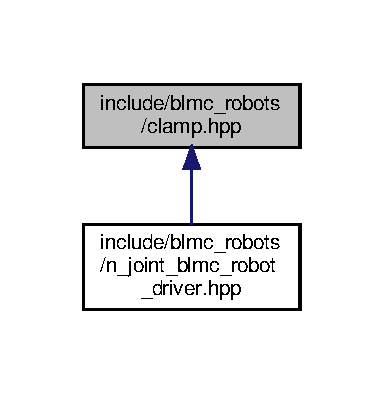
\includegraphics[width=184pt]{clamp_8hpp__dep__incl}
\end{center}
\end{figure}
\subsection*{Functions}
\begin{DoxyCompactItemize}
\item 
{\footnotesize template$<$typename Vector $>$ }\\Vector \hyperlink{clamp_8hpp_a00195e5b1ad14316624d026f7e590ad1}{blmc\+\_\+robots\+::clamp} (const Vector \&vector, const double lower\+\_\+limit, const double upper\+\_\+limit)
\begin{DoxyCompactList}\small\item\em Clamp an arbitrary Eigen vector. \end{DoxyCompactList}\end{DoxyCompactItemize}


\subsection{Detailed Description}
\begin{DoxyCopyright}{Copyright}
Copyright (c) 2020, New York University \& Max Planck Gesellschaft. 
\end{DoxyCopyright}


\subsection{Function Documentation}
\mbox{\Hypertarget{clamp_8hpp_file_a00195e5b1ad14316624d026f7e590ad1}\label{clamp_8hpp_file_a00195e5b1ad14316624d026f7e590ad1}} 
\index{clamp.\+hpp@{clamp.\+hpp}!clamp@{clamp}}
\index{clamp@{clamp}!clamp.\+hpp@{clamp.\+hpp}}
\subsubsection{\texorpdfstring{clamp()}{clamp()}}
{\footnotesize\ttfamily template$<$typename Vector $>$ \\
Vector blmc\+\_\+robots\+::clamp (\begin{DoxyParamCaption}\item[{const Vector \&}]{vector,  }\item[{const double}]{lower\+\_\+limit,  }\item[{const double}]{upper\+\_\+limit }\end{DoxyParamCaption})}



Clamp an arbitrary Eigen vector. 


\begin{DoxyParams}{Parameters}
{\em vector} & The vector that is to be clamped. \\
\hline
{\em lower\+\_\+limit} & Lower limit. \\
\hline
{\em upper\+\_\+limit} & Upper limit.\\
\hline
\end{DoxyParams}
\begin{DoxyReturn}{Returns}
Copy of vector where values below or above the limits are set to the corresponding limit values. 
\end{DoxyReturn}

\hypertarget{common__header_8hpp}{}\section{include/blmc\+\_\+robots/common\+\_\+header.hpp File Reference}
\label{common__header_8hpp}\index{include/blmc\+\_\+robots/common\+\_\+header.\+hpp@{include/blmc\+\_\+robots/common\+\_\+header.\+hpp}}


The hardware wrapper of the quadruped.  


{\ttfamily \#include \char`\"{}yaml\+\_\+cpp\+\_\+catkin/yaml\+\_\+cpp\+\_\+fwd.\+hpp\char`\"{}}\newline
{\ttfamily \#include $<$Eigen/\+Eigen$>$}\newline
{\ttfamily \#include $<$signal.\+h$>$}\newline
{\ttfamily \#include $<$atomic$>$}\newline
{\ttfamily \#include \char`\"{}real\+\_\+time\+\_\+tools/iostream.\+hpp\char`\"{}}\newline
{\ttfamily \#include \char`\"{}real\+\_\+time\+\_\+tools/spinner.\+hpp\char`\"{}}\newline
{\ttfamily \#include \char`\"{}real\+\_\+time\+\_\+tools/thread.\+hpp\char`\"{}}\newline
{\ttfamily \#include \char`\"{}real\+\_\+time\+\_\+tools/timer.\+hpp\char`\"{}}\newline
{\ttfamily \#include $<$blmc\+\_\+drivers/devices/analog\+\_\+sensor.\+hpp$>$}\newline
{\ttfamily \#include $<$blmc\+\_\+drivers/devices/motor.\+hpp$>$}\newline
Include dependency graph for common\+\_\+header.\+hpp\+:
\nopagebreak
\begin{figure}[H]
\begin{center}
\leavevmode
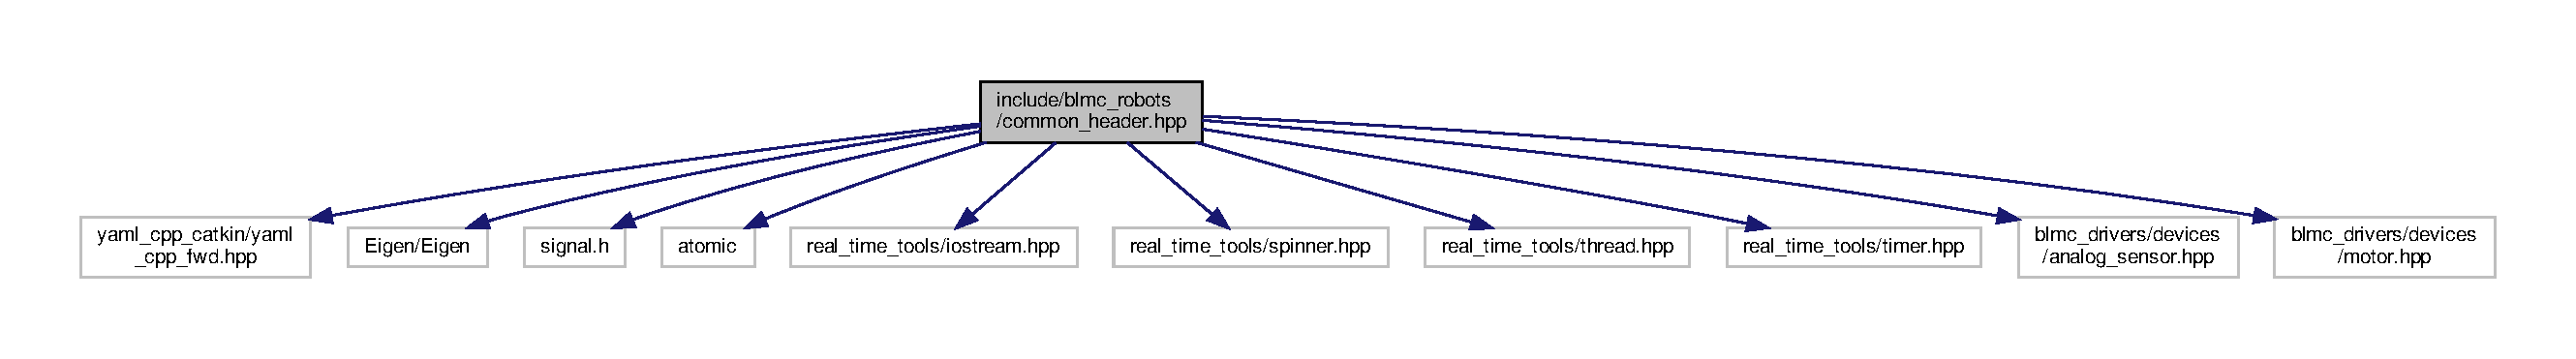
\includegraphics[width=350pt]{common__header_8hpp__incl}
\end{center}
\end{figure}
This graph shows which files directly or indirectly include this file\+:
\nopagebreak
\begin{figure}[H]
\begin{center}
\leavevmode
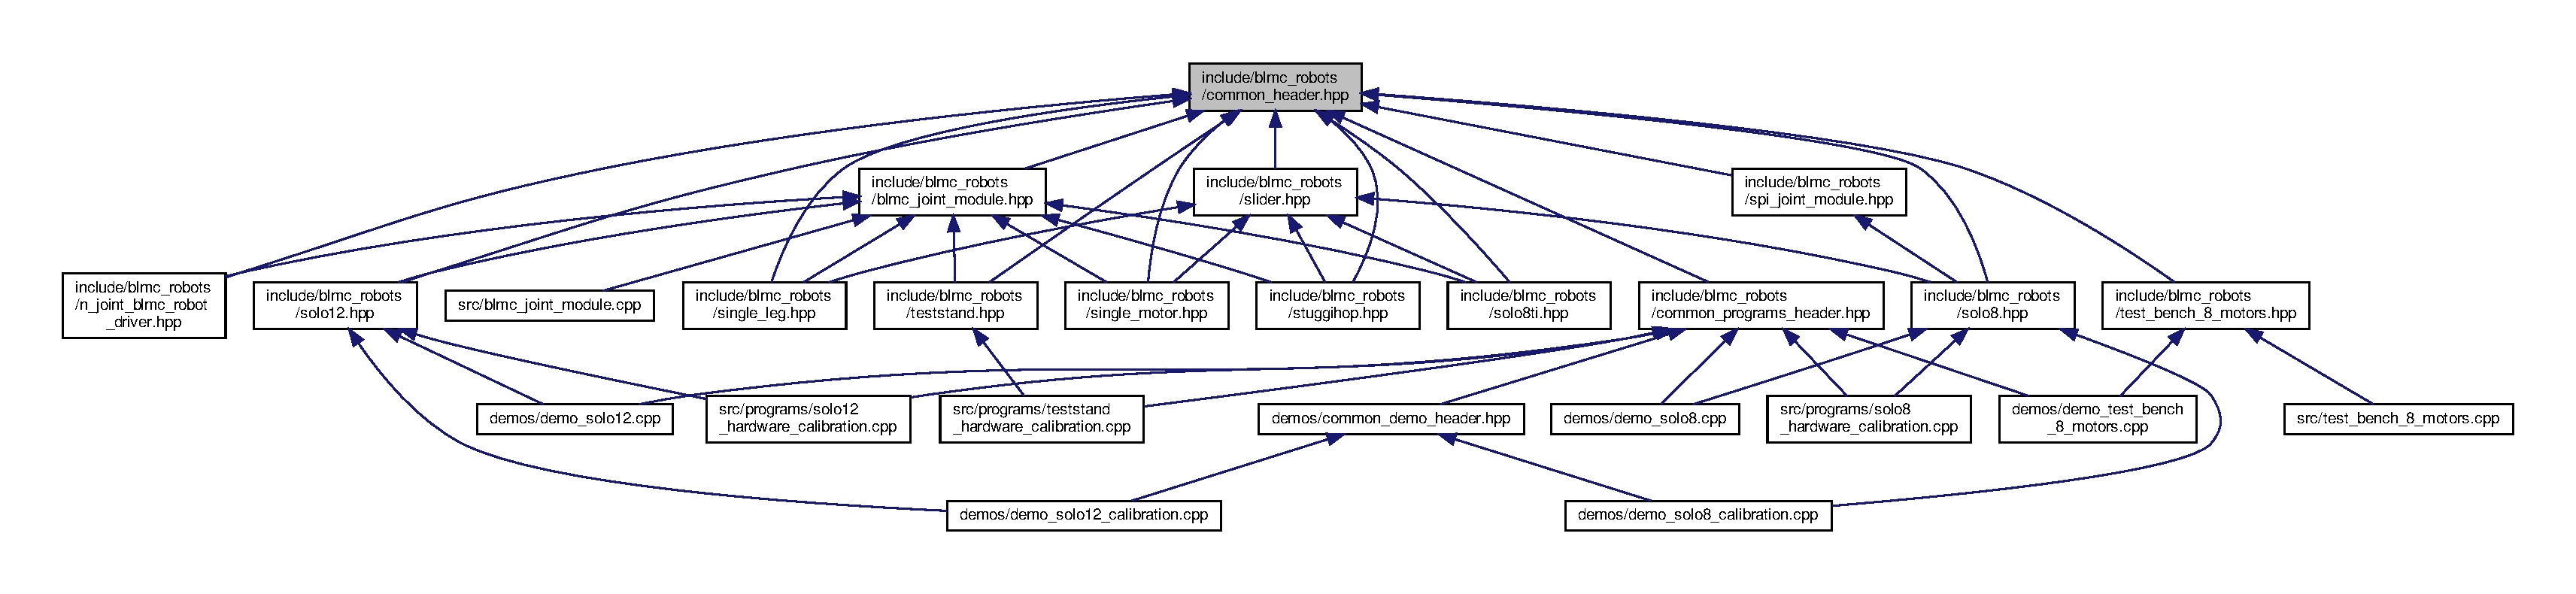
\includegraphics[width=350pt]{common__header_8hpp__dep__incl}
\end{center}
\end{figure}
\subsection*{Typedefs}
\begin{DoxyCompactItemize}
\item 
\mbox{\Hypertarget{common__header_8hpp_a932c1319d78144ebcaa8938ae070b784}\label{common__header_8hpp_a932c1319d78144ebcaa8938ae070b784}} 
typedef Eigen\+::\+Matrix$<$ double, 1, 1 $>$ \hyperlink{common__header_8hpp_a932c1319d78144ebcaa8938ae070b784}{blmc\+\_\+robots\+::\+Vector1d}
\begin{DoxyCompactList}\small\item\em Vector2d shortcut for the eigen vector of size 1. \end{DoxyCompactList}\item 
\mbox{\Hypertarget{common__header_8hpp_acb6916bc8c9fe9d98c484fd4cc201447}\label{common__header_8hpp_acb6916bc8c9fe9d98c484fd4cc201447}} 
typedef Eigen\+::\+Matrix$<$ double, 2, 1 $>$ \hyperlink{common__header_8hpp_acb6916bc8c9fe9d98c484fd4cc201447}{blmc\+\_\+robots\+::\+Vector2d}
\begin{DoxyCompactList}\small\item\em Vector2d shortcut for the eigen vector of size 2. \end{DoxyCompactList}\item 
\mbox{\Hypertarget{common__header_8hpp_ac3c26fc5a016ed8f49235f2b3cd38aa2}\label{common__header_8hpp_ac3c26fc5a016ed8f49235f2b3cd38aa2}} 
typedef Eigen\+::\+Matrix$<$ double, 6, 1 $>$ \hyperlink{common__header_8hpp_ac3c26fc5a016ed8f49235f2b3cd38aa2}{blmc\+\_\+robots\+::\+Vector6d}
\begin{DoxyCompactList}\small\item\em Vector2d shortcut for the eigen vector of size 6. \end{DoxyCompactList}\item 
\mbox{\Hypertarget{common__header_8hpp_a98975ffbe0bca1296078e0350dfedd60}\label{common__header_8hpp_a98975ffbe0bca1296078e0350dfedd60}} 
typedef Eigen\+::\+Matrix$<$ double, 8, 1 $>$ \hyperlink{common__header_8hpp_a98975ffbe0bca1296078e0350dfedd60}{blmc\+\_\+robots\+::\+Vector8d}
\begin{DoxyCompactList}\small\item\em Vector8d shortcut for the eigen vector of size 8. \end{DoxyCompactList}\item 
\mbox{\Hypertarget{common__header_8hpp_a80313eb420184518596e745eecf4b494}\label{common__header_8hpp_a80313eb420184518596e745eecf4b494}} 
typedef Eigen\+::\+Matrix$<$ double, 12, 1 $>$ \hyperlink{common__header_8hpp_a80313eb420184518596e745eecf4b494}{blmc\+\_\+robots\+::\+Vector12d}
\begin{DoxyCompactList}\small\item\em Vector8d shortcut for the eigen vector of size 12. \end{DoxyCompactList}\item 
\mbox{\Hypertarget{common__header_8hpp_a793c8789a7598e8aaf766939da7262af}\label{common__header_8hpp_a793c8789a7598e8aaf766939da7262af}} 
typedef std\+::shared\+\_\+ptr$<$ blmc\+\_\+drivers\+::\+Can\+Bus $>$ \hyperlink{common__header_8hpp_a793c8789a7598e8aaf766939da7262af}{blmc\+\_\+robots\+::\+Can\+Bus\+\_\+ptr}
\begin{DoxyCompactList}\small\item\em Can\+Bus\+\_\+ptr shortcut for the shared pointer Can\+Bus type. \end{DoxyCompactList}\item 
\mbox{\Hypertarget{common__header_8hpp_aab1c6ddb1273247a1b45d5e8b417c216}\label{common__header_8hpp_aab1c6ddb1273247a1b45d5e8b417c216}} 
typedef std\+::shared\+\_\+ptr$<$ blmc\+\_\+drivers\+::\+Can\+Bus\+Motor\+Board $>$ \hyperlink{common__header_8hpp_aab1c6ddb1273247a1b45d5e8b417c216}{blmc\+\_\+robots\+::\+Can\+Bus\+Motor\+Board\+\_\+ptr}
\begin{DoxyCompactList}\small\item\em Can\+Bus\+Motor\+Board\+\_\+\+Ptr shortcut for the shared pointer Can\+Bus type. \end{DoxyCompactList}\item 
\mbox{\Hypertarget{common__header_8hpp_ae1a0f9992bc8fbbc1943d887f517c180}\label{common__header_8hpp_ae1a0f9992bc8fbbc1943d887f517c180}} 
typedef std\+::shared\+\_\+ptr$<$ blmc\+\_\+drivers\+::\+Motor\+Interface $>$ \hyperlink{common__header_8hpp_ae1a0f9992bc8fbbc1943d887f517c180}{blmc\+\_\+robots\+::\+Motor\+Interface\+\_\+ptr}
\begin{DoxyCompactList}\small\item\em Motor\+Interface\+\_\+ptr shortcut for the shared pointer Motor\+Interface type. \end{DoxyCompactList}\item 
\mbox{\Hypertarget{common__header_8hpp_aeba0df1e898326cde4922419d871c5c6}\label{common__header_8hpp_aeba0df1e898326cde4922419d871c5c6}} 
typedef std\+::shared\+\_\+ptr$<$ blmc\+\_\+drivers\+::\+Motor $>$ \hyperlink{common__header_8hpp_aeba0df1e898326cde4922419d871c5c6}{blmc\+\_\+robots\+::\+Motor\+\_\+ptr}
\begin{DoxyCompactList}\small\item\em Motor\+\_\+ptr shortcut for the shared pointer Motor type. \end{DoxyCompactList}\item 
\mbox{\Hypertarget{common__header_8hpp_a9850cf917156e20846aef3f8195aea0f}\label{common__header_8hpp_a9850cf917156e20846aef3f8195aea0f}} 
typedef std\+::shared\+\_\+ptr$<$ blmc\+\_\+drivers\+::\+Safe\+Motor $>$ \hyperlink{common__header_8hpp_a9850cf917156e20846aef3f8195aea0f}{blmc\+\_\+robots\+::\+Safe\+Motor\+\_\+ptr}
\begin{DoxyCompactList}\small\item\em Safe\+Motor\+\_\+ptr shortcut for the shared pointer Safe\+Motor type. \end{DoxyCompactList}\item 
\mbox{\Hypertarget{common__header_8hpp_a4cb9a95e8b2c0bf237ce29f5252c7b73}\label{common__header_8hpp_a4cb9a95e8b2c0bf237ce29f5252c7b73}} 
typedef std\+::shared\+\_\+ptr$<$ blmc\+\_\+drivers\+::\+Analog\+Sensor $>$ \hyperlink{common__header_8hpp_a4cb9a95e8b2c0bf237ce29f5252c7b73}{blmc\+\_\+robots\+::\+Slider\+\_\+ptr}
\begin{DoxyCompactList}\small\item\em Slider\+\_\+ptr shortcut for the linear potentiometer analog sensor. \end{DoxyCompactList}\item 
typedef std\+::shared\+\_\+ptr$<$ blmc\+\_\+drivers\+::\+Analog\+Sensor $>$ \hyperlink{common__header_8hpp_ac78fe5c68e56a3b884117109959e4d58}{blmc\+\_\+robots\+::\+Contact\+Sensor\+\_\+ptr}
\begin{DoxyCompactList}\small\item\em Contact\+Sensor\+\_\+ptr shortcut for the contact sensor. \end{DoxyCompactList}\item 
typedef std\+::shared\+\_\+ptr$<$ blmc\+\_\+drivers\+::\+Analog\+Sensor $>$ \hyperlink{common__header_8hpp_a921d3f5a8878524375bf7e740f2fb788}{blmc\+\_\+robots\+::\+Height\+Sensor\+\_\+ptr}
\begin{DoxyCompactList}\small\item\em Height\+Sensor\+\_\+ptr shortcut for the height sensor. \end{DoxyCompactList}\item 
\mbox{\Hypertarget{common__header_8hpp_a1975c6bb47bc85dfc8edfe349c30dae1}\label{common__header_8hpp_a1975c6bb47bc85dfc8edfe349c30dae1}} 
typedef blmc\+\_\+drivers\+::\+Motor\+Interface\+::\+Measurement\+Index \hyperlink{common__header_8hpp_a1975c6bb47bc85dfc8edfe349c30dae1}{blmc\+\_\+robots\+::mi}
\begin{DoxyCompactList}\small\item\em mi, this typedef is used to get the measurements from the blmc api \end{DoxyCompactList}\end{DoxyCompactItemize}


\subsection{Detailed Description}
The hardware wrapper of the quadruped. 

\begin{DoxyAuthor}{Author}
Maximilien Naveau 
\end{DoxyAuthor}
\begin{DoxyDate}{Date}
2018
\end{DoxyDate}
This file declares the Test\+Bench8\+Motors class which defines the test bench with 8 motors. 

\subsection{Typedef Documentation}
\mbox{\Hypertarget{common__header_8hpp_file_ac78fe5c68e56a3b884117109959e4d58}\label{common__header_8hpp_file_ac78fe5c68e56a3b884117109959e4d58}} 
\index{common\+\_\+header.\+hpp@{common\+\_\+header.\+hpp}!Contact\+Sensor\+\_\+ptr@{Contact\+Sensor\+\_\+ptr}}
\index{Contact\+Sensor\+\_\+ptr@{Contact\+Sensor\+\_\+ptr}!common\+\_\+header.\+hpp@{common\+\_\+header.\+hpp}}
\subsubsection{\texorpdfstring{Contact\+Sensor\+\_\+ptr}{ContactSensor\_ptr}}
{\footnotesize\ttfamily typedef std\+::shared\+\_\+ptr$<$blmc\+\_\+drivers\+::\+Analog\+Sensor$>$ \hyperlink{common__header_8hpp_ac78fe5c68e56a3b884117109959e4d58}{blmc\+\_\+robots\+::\+Contact\+Sensor\+\_\+ptr}}



Contact\+Sensor\+\_\+ptr shortcut for the contact sensor. 

It is also an analog sensor \mbox{\Hypertarget{common__header_8hpp_file_a921d3f5a8878524375bf7e740f2fb788}\label{common__header_8hpp_file_a921d3f5a8878524375bf7e740f2fb788}} 
\index{common\+\_\+header.\+hpp@{common\+\_\+header.\+hpp}!Height\+Sensor\+\_\+ptr@{Height\+Sensor\+\_\+ptr}}
\index{Height\+Sensor\+\_\+ptr@{Height\+Sensor\+\_\+ptr}!common\+\_\+header.\+hpp@{common\+\_\+header.\+hpp}}
\subsubsection{\texorpdfstring{Height\+Sensor\+\_\+ptr}{HeightSensor\_ptr}}
{\footnotesize\ttfamily typedef std\+::shared\+\_\+ptr$<$blmc\+\_\+drivers\+::\+Analog\+Sensor$>$ \hyperlink{common__header_8hpp_a921d3f5a8878524375bf7e740f2fb788}{blmc\+\_\+robots\+::\+Height\+Sensor\+\_\+ptr}}



Height\+Sensor\+\_\+ptr shortcut for the height sensor. 

It is also an analog sensor 
\hypertarget{polynome_8hpp}{}\section{include/blmc\+\_\+robots/mathematics/polynome.hpp File Reference}
\label{polynome_8hpp}\index{include/blmc\+\_\+robots/mathematics/polynome.\+hpp@{include/blmc\+\_\+robots/mathematics/polynome.\+hpp}}


Polynomes object for trajectories.  


{\ttfamily \#include $<$array$>$}\newline
{\ttfamily \#include \char`\"{}blmc\+\_\+robots/mathematics/polynome.\+hxx\char`\"{}}\newline
Include dependency graph for polynome.\+hpp\+:
\nopagebreak
\begin{figure}[H]
\begin{center}
\leavevmode
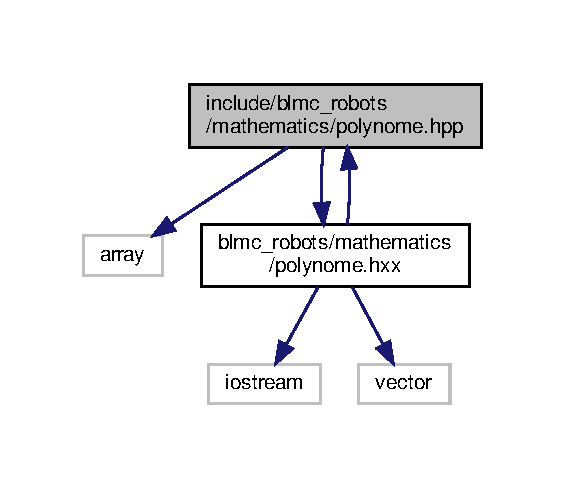
\includegraphics[width=271pt]{polynome_8hpp__incl}
\end{center}
\end{figure}
This graph shows which files directly or indirectly include this file\+:
\nopagebreak
\begin{figure}[H]
\begin{center}
\leavevmode
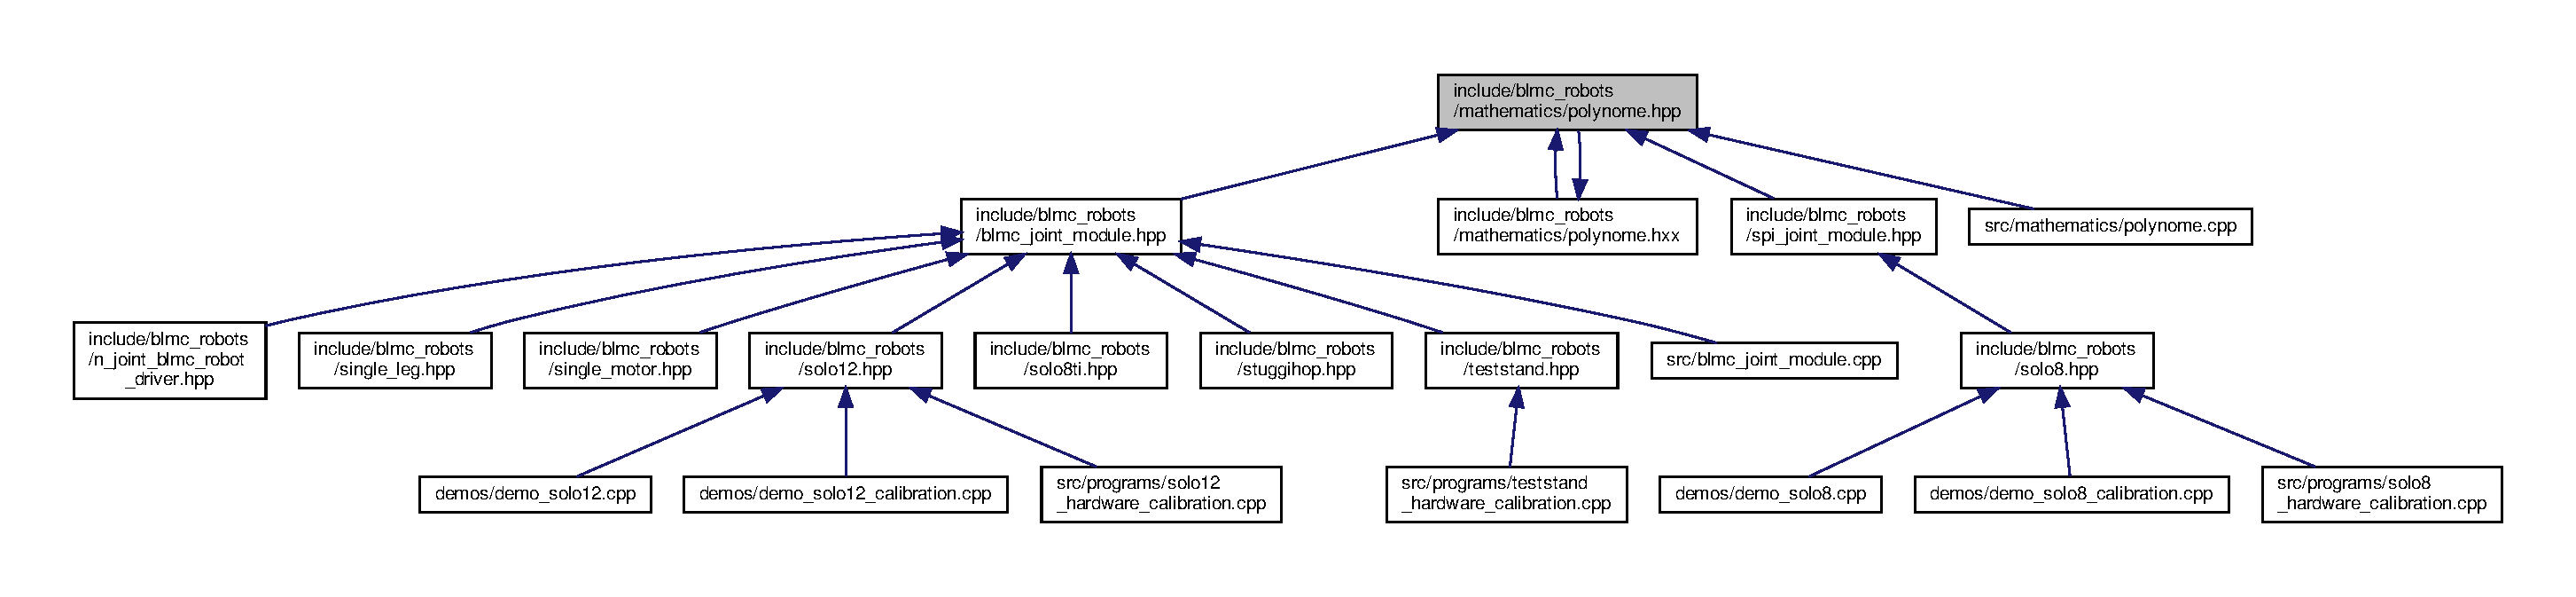
\includegraphics[width=350pt]{polynome_8hpp__dep__incl}
\end{center}
\end{figure}
\subsection*{Classes}
\begin{DoxyCompactItemize}
\item 
class \hyperlink{classblmc__robots_1_1Polynome}{blmc\+\_\+robots\+::\+Polynome$<$ O\+R\+D\+E\+R $>$}
\begin{DoxyCompactList}\small\item\em Simple class that defines $ P(x) $ a polynome of order O\+R\+D\+ER. \end{DoxyCompactList}\item 
class \hyperlink{classblmc__robots_1_1TimePolynome}{blmc\+\_\+robots\+::\+Time\+Polynome$<$ O\+R\+D\+E\+R $>$}
\begin{DoxyCompactList}\small\item\em Simple class that defines $ P(t) $ a polynome of order O\+R\+D\+ER. \end{DoxyCompactList}\end{DoxyCompactItemize}


\subsection{Detailed Description}
Polynomes object for trajectories. 

\begin{DoxyAuthor}{Author}
Maximilien Naveau (\href{mailto:maximilien.naveau@gmail.com}{\tt maximilien.\+naveau@gmail.\+com}) 
\end{DoxyAuthor}
\begin{DoxyVersion}{Version}
0.\+1 
\end{DoxyVersion}
\begin{DoxyDate}{Date}
2019-\/11-\/06
\end{DoxyDate}
\begin{DoxyCopyright}{Copyright}
Copyright (c) 2019 
\end{DoxyCopyright}

\hypertarget{n__joint__blmc__robot__driver_8hpp}{}\section{include/blmc\+\_\+robots/n\+\_\+joint\+\_\+blmc\+\_\+robot\+\_\+driver.hpp File Reference}
\label{n__joint__blmc__robot__driver_8hpp}\index{include/blmc\+\_\+robots/n\+\_\+joint\+\_\+blmc\+\_\+robot\+\_\+driver.\+hpp@{include/blmc\+\_\+robots/n\+\_\+joint\+\_\+blmc\+\_\+robot\+\_\+driver.\+hpp}}


Base driver for a generic n-\/joint B\+L\+MC robot.  


{\ttfamily \#include $<$array$>$}\newline
{\ttfamily \#include $<$cmath$>$}\newline
{\ttfamily \#include $<$iterator$>$}\newline
{\ttfamily \#include $<$string$>$}\newline
{\ttfamily \#include $<$yaml-\/cpp/yaml.\+h$>$}\newline
{\ttfamily \#include $<$Eigen/\+Eigen$>$}\newline
{\ttfamily \#include $<$yaml\+\_\+cpp\+\_\+catkin/yaml\+\_\+eigen.\+h$>$}\newline
{\ttfamily \#include $<$robot\+\_\+interfaces/monitored\+\_\+robot\+\_\+driver.\+hpp$>$}\newline
{\ttfamily \#include $<$robot\+\_\+interfaces/n\+\_\+joint\+\_\+robot\+\_\+types.\+hpp$>$}\newline
{\ttfamily \#include $<$robot\+\_\+interfaces/robot\+\_\+driver.\+hpp$>$}\newline
{\ttfamily \#include $<$blmc\+\_\+robots/blmc\+\_\+joint\+\_\+module.\+hpp$>$}\newline
{\ttfamily \#include $<$blmc\+\_\+robots/clamp.\+hpp$>$}\newline
{\ttfamily \#include $<$blmc\+\_\+robots/common\+\_\+header.\+hpp$>$}\newline
{\ttfamily \#include \char`\"{}n\+\_\+joint\+\_\+blmc\+\_\+robot\+\_\+driver.\+hxx\char`\"{}}\newline
Include dependency graph for n\+\_\+joint\+\_\+blmc\+\_\+robot\+\_\+driver.\+hpp\+:
\nopagebreak
\begin{figure}[H]
\begin{center}
\leavevmode
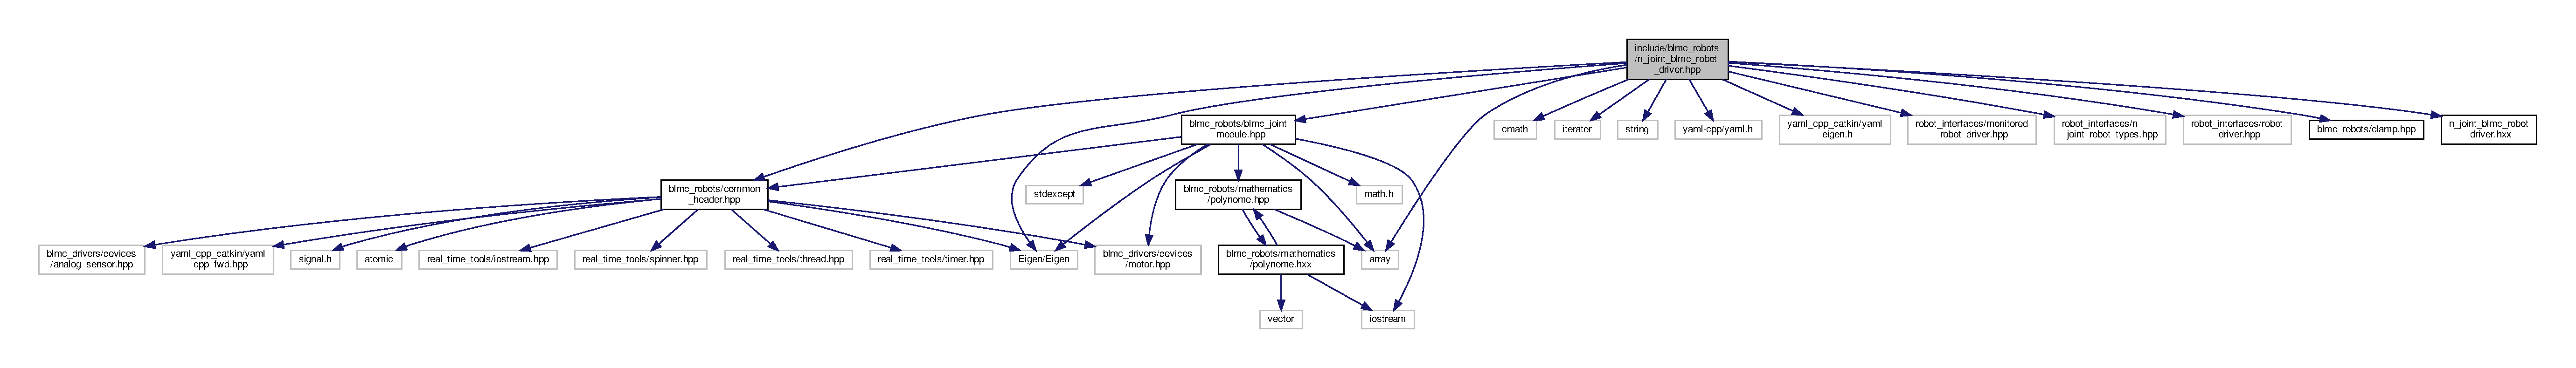
\includegraphics[width=350pt]{n__joint__blmc__robot__driver_8hpp__incl}
\end{center}
\end{figure}
\subsection*{Classes}
\begin{DoxyCompactItemize}
\item 
struct \hyperlink{structblmc__robots_1_1MotorParameters}{blmc\+\_\+robots\+::\+Motor\+Parameters}
\begin{DoxyCompactList}\small\item\em Parameters related to the motor. \end{DoxyCompactList}\item 
class \hyperlink{classblmc__robots_1_1NJointBlmcRobotDriver}{blmc\+\_\+robots\+::\+N\+Joint\+Blmc\+Robot\+Driver$<$ Observation, N\+\_\+\+J\+O\+I\+N\+T\+S, N\+\_\+\+M\+O\+T\+O\+R\+\_\+\+B\+O\+A\+R\+D\+S $>$}
\begin{DoxyCompactList}\small\item\em Base class for n-\/joint B\+L\+MC robots. \end{DoxyCompactList}\item 
struct \hyperlink{structblmc__robots_1_1NJointBlmcRobotDriver_1_1Config}{blmc\+\_\+robots\+::\+N\+Joint\+Blmc\+Robot\+Driver$<$ Observation, N\+\_\+\+J\+O\+I\+N\+T\+S, N\+\_\+\+M\+O\+T\+O\+R\+\_\+\+B\+O\+A\+R\+D\+S $>$\+::\+Config}
\begin{DoxyCompactList}\small\item\em Configuration of the robot that can be changed by the user. \end{DoxyCompactList}\item 
struct \hyperlink{structblmc__robots_1_1NJointBlmcRobotDriver_1_1Config_1_1TrajectoryStep}{blmc\+\_\+robots\+::\+N\+Joint\+Blmc\+Robot\+Driver$<$ Observation, N\+\_\+\+J\+O\+I\+N\+T\+S, N\+\_\+\+M\+O\+T\+O\+R\+\_\+\+B\+O\+A\+R\+D\+S $>$\+::\+Config\+::\+Trajectory\+Step}
\begin{DoxyCompactList}\small\item\em A sub-\/goal of a trajectory. \end{DoxyCompactList}\item 
class \hyperlink{classblmc__robots_1_1SimpleNJointBlmcRobotDriver}{blmc\+\_\+robots\+::\+Simple\+N\+Joint\+Blmc\+Robot\+Driver$<$ N\+\_\+\+J\+O\+I\+N\+T\+S, N\+\_\+\+M\+O\+T\+O\+R\+\_\+\+B\+O\+A\+R\+D\+S $>$}
\begin{DoxyCompactList}\small\item\em Simple n-\/joint robot driver that uses N\+Joint\+Observation. \end{DoxyCompactList}\end{DoxyCompactItemize}
\subsection*{Functions}
\begin{DoxyCompactItemize}
\item 
{\footnotesize template$<$typename Driver $>$ }\\Driver\+::\+Types\+::\+Backend\+Ptr \hyperlink{n__joint__blmc__robot__driver_8hpp_a988c07200135ba12bf9ec1bbe955bde8}{blmc\+\_\+robots\+::create\+\_\+backend} (typename Driver\+::\+Types\+::\+Base\+Data\+Ptr robot\+\_\+data, const std\+::string \&config\+\_\+file\+\_\+path, const double first\+\_\+action\+\_\+timeout=std\+::numeric\+\_\+limits$<$ double $>$\+::infinity())
\begin{DoxyCompactList}\small\item\em Create backend using the specified driver. \end{DoxyCompactList}\end{DoxyCompactItemize}


\subsection{Detailed Description}
Base driver for a generic n-\/joint B\+L\+MC robot. 

\begin{DoxyCopyright}{Copyright}
Copyright (c) 2019, New York University and Max Planck Gesellschaft. 
\end{DoxyCopyright}


\subsection{Function Documentation}
\mbox{\Hypertarget{n__joint__blmc__robot__driver_8hpp_file_a988c07200135ba12bf9ec1bbe955bde8}\label{n__joint__blmc__robot__driver_8hpp_file_a988c07200135ba12bf9ec1bbe955bde8}} 
\index{n\+\_\+joint\+\_\+blmc\+\_\+robot\+\_\+driver.\+hpp@{n\+\_\+joint\+\_\+blmc\+\_\+robot\+\_\+driver.\+hpp}!create\+\_\+backend@{create\+\_\+backend}}
\index{create\+\_\+backend@{create\+\_\+backend}!n\+\_\+joint\+\_\+blmc\+\_\+robot\+\_\+driver.\+hpp@{n\+\_\+joint\+\_\+blmc\+\_\+robot\+\_\+driver.\+hpp}}
\subsubsection{\texorpdfstring{create\+\_\+backend()}{create\_backend()}}
{\footnotesize\ttfamily template$<$typename Driver $>$ \\
Driver\+::\+Types\+::\+Backend\+Ptr blmc\+\_\+robots\+::create\+\_\+backend (\begin{DoxyParamCaption}\item[{typename Driver\+::\+Types\+::\+Base\+Data\+Ptr}]{robot\+\_\+data,  }\item[{const std\+::string \&}]{config\+\_\+file\+\_\+path,  }\item[{const double}]{first\+\_\+action\+\_\+timeout = {\ttfamily std\+:\+:numeric\+\_\+limits$<$double$>$\+:\+:infinity()} }\end{DoxyParamCaption})}



Create backend using the specified driver. 


\begin{DoxyTemplParams}{Template Parameters}
{\em Driver} & Type of the driver. Expected to inherit from N\+Joint\+Blmc\+Robot\+Driver.\\
\hline
\end{DoxyTemplParams}

\begin{DoxyParams}{Parameters}
{\em robot\+\_\+data} & Instance of Robot\+Data used for communication. \\
\hline
{\em config\+\_\+file\+\_\+path} & Path to the driver configuration file. \\
\hline
{\em first\+\_\+action\+\_\+timeout} & Duration for which the backend waits for the first action to arrive. If exceeded, the backend shuts down.\\
\hline
\end{DoxyParams}
\begin{DoxyReturn}{Returns}
A Robot\+Backend instances with a driver of the specified type. 
\end{DoxyReturn}

\hypertarget{n__joint__blmc__robot__driver_8hxx}{}\section{include/blmc\+\_\+robots/n\+\_\+joint\+\_\+blmc\+\_\+robot\+\_\+driver.hxx File Reference}
\label{n__joint__blmc__robot__driver_8hxx}\index{include/blmc\+\_\+robots/n\+\_\+joint\+\_\+blmc\+\_\+robot\+\_\+driver.\+hxx@{include/blmc\+\_\+robots/n\+\_\+joint\+\_\+blmc\+\_\+robot\+\_\+driver.\+hxx}}


Base driver for a generic n-\/joint B\+L\+MC robot.  


This graph shows which files directly or indirectly include this file\+:
\nopagebreak
\begin{figure}[H]
\begin{center}
\leavevmode
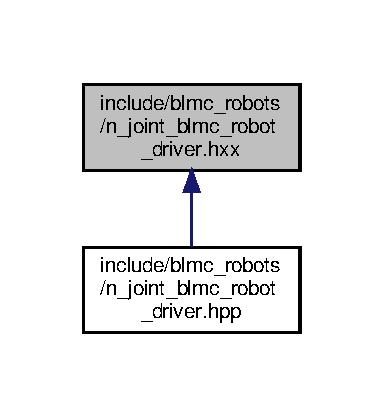
\includegraphics[width=184pt]{n__joint__blmc__robot__driver_8hxx__dep__incl}
\end{center}
\end{figure}
\subsection*{Macros}
\begin{DoxyCompactItemize}
\item 
\mbox{\Hypertarget{n__joint__blmc__robot__driver_8hxx_af909d89428f53da32679d03618b311d1}\label{n__joint__blmc__robot__driver_8hxx_af909d89428f53da32679d03618b311d1}} 
\#define {\bfseries T\+P\+L\+\_\+\+N\+J\+B\+RD}~template $<$typename Observation, size\+\_\+t N\+\_\+\+J\+O\+I\+N\+TS, size\+\_\+t N\+\_\+\+M\+O\+T\+O\+R\+\_\+\+B\+O\+A\+R\+DS$>$
\item 
\mbox{\Hypertarget{n__joint__blmc__robot__driver_8hxx_ac2cdeca7fcd08f342bed16bc324fcf04}\label{n__joint__blmc__robot__driver_8hxx_ac2cdeca7fcd08f342bed16bc324fcf04}} 
\#define {\bfseries N\+J\+B\+RD}~N\+Joint\+Blmc\+Robot\+Driver$<$Observation, N\+\_\+\+J\+O\+I\+N\+TS, N\+\_\+\+M\+O\+T\+O\+R\+\_\+\+B\+O\+A\+R\+DS$>$
\end{DoxyCompactItemize}


\subsection{Detailed Description}
Base driver for a generic n-\/joint B\+L\+MC robot. 

\begin{DoxyCopyright}{Copyright}
Copyright (c) 2019, New York University and Max Planck Gesellschaft. 
\end{DoxyCopyright}

\hypertarget{single__leg_8hpp}{}\section{include/blmc\+\_\+robots/single\+\_\+leg.hpp File Reference}
\label{single__leg_8hpp}\index{include/blmc\+\_\+robots/single\+\_\+leg.\+hpp@{include/blmc\+\_\+robots/single\+\_\+leg.\+hpp}}


The hardware wrapper of the Real\+Finger.  


{\ttfamily \#include $<$blmc\+\_\+robots/blmc\+\_\+joint\+\_\+module.\+hpp$>$}\newline
{\ttfamily \#include $<$blmc\+\_\+robots/common\+\_\+header.\+hpp$>$}\newline
{\ttfamily \#include $<$blmc\+\_\+robots/slider.\+hpp$>$}\newline
Include dependency graph for single\+\_\+leg.\+hpp\+:
\nopagebreak
\begin{figure}[H]
\begin{center}
\leavevmode
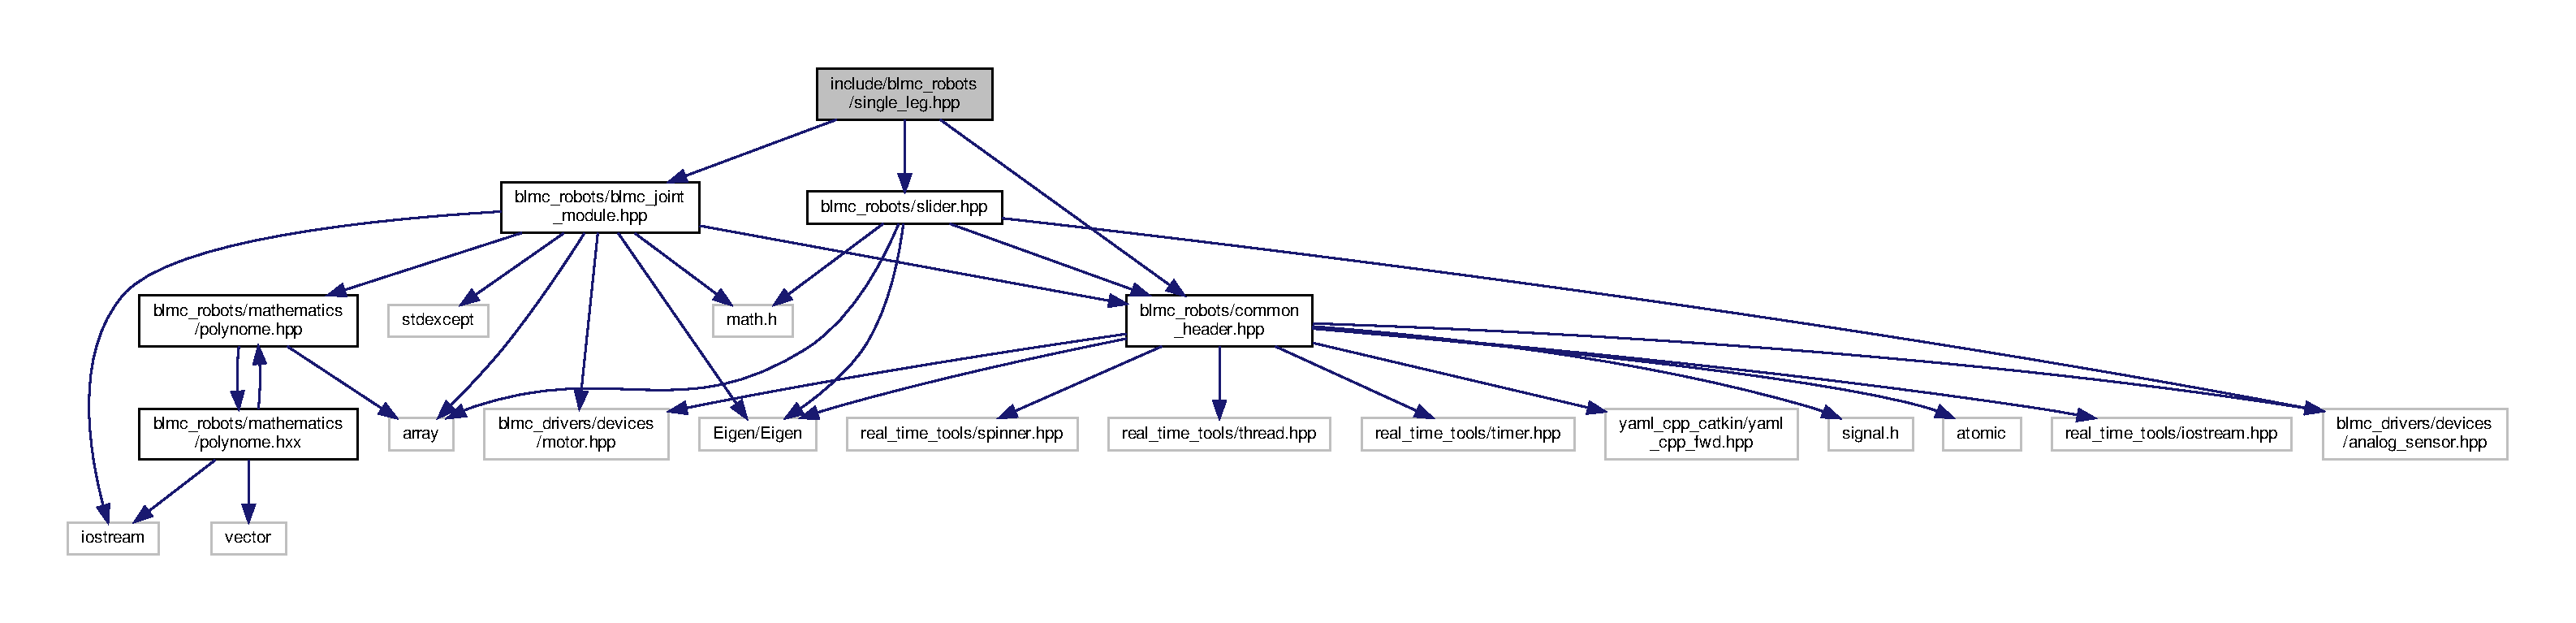
\includegraphics[width=350pt]{single__leg_8hpp__incl}
\end{center}
\end{figure}
\subsection*{Classes}
\begin{DoxyCompactItemize}
\item 
class \hyperlink{classblmc__robots_1_1SingleLeg}{blmc\+\_\+robots\+::\+Single\+Leg}
\end{DoxyCompactItemize}


\subsection{Detailed Description}
The hardware wrapper of the Real\+Finger. 

\begin{DoxyAuthor}{Author}
Manuel Wuthrich 
\end{DoxyAuthor}
\begin{DoxyDate}{Date}
2018 
\end{DoxyDate}
\begin{DoxyCopyright}{Copyright}
Copyright (c) 2019, New York University \& Max Planck Gesellschaft. 
\end{DoxyCopyright}

\hypertarget{single__motor_8hpp}{}\section{include/blmc\+\_\+robots/single\+\_\+motor.hpp File Reference}
\label{single__motor_8hpp}\index{include/blmc\+\_\+robots/single\+\_\+motor.\+hpp@{include/blmc\+\_\+robots/single\+\_\+motor.\+hpp}}
{\ttfamily \#include $<$blmc\+\_\+robots/blmc\+\_\+joint\+\_\+module.\+hpp$>$}\newline
{\ttfamily \#include $<$blmc\+\_\+robots/common\+\_\+header.\+hpp$>$}\newline
{\ttfamily \#include $<$blmc\+\_\+robots/slider.\+hpp$>$}\newline
Include dependency graph for single\+\_\+motor.\+hpp\+:
\nopagebreak
\begin{figure}[H]
\begin{center}
\leavevmode
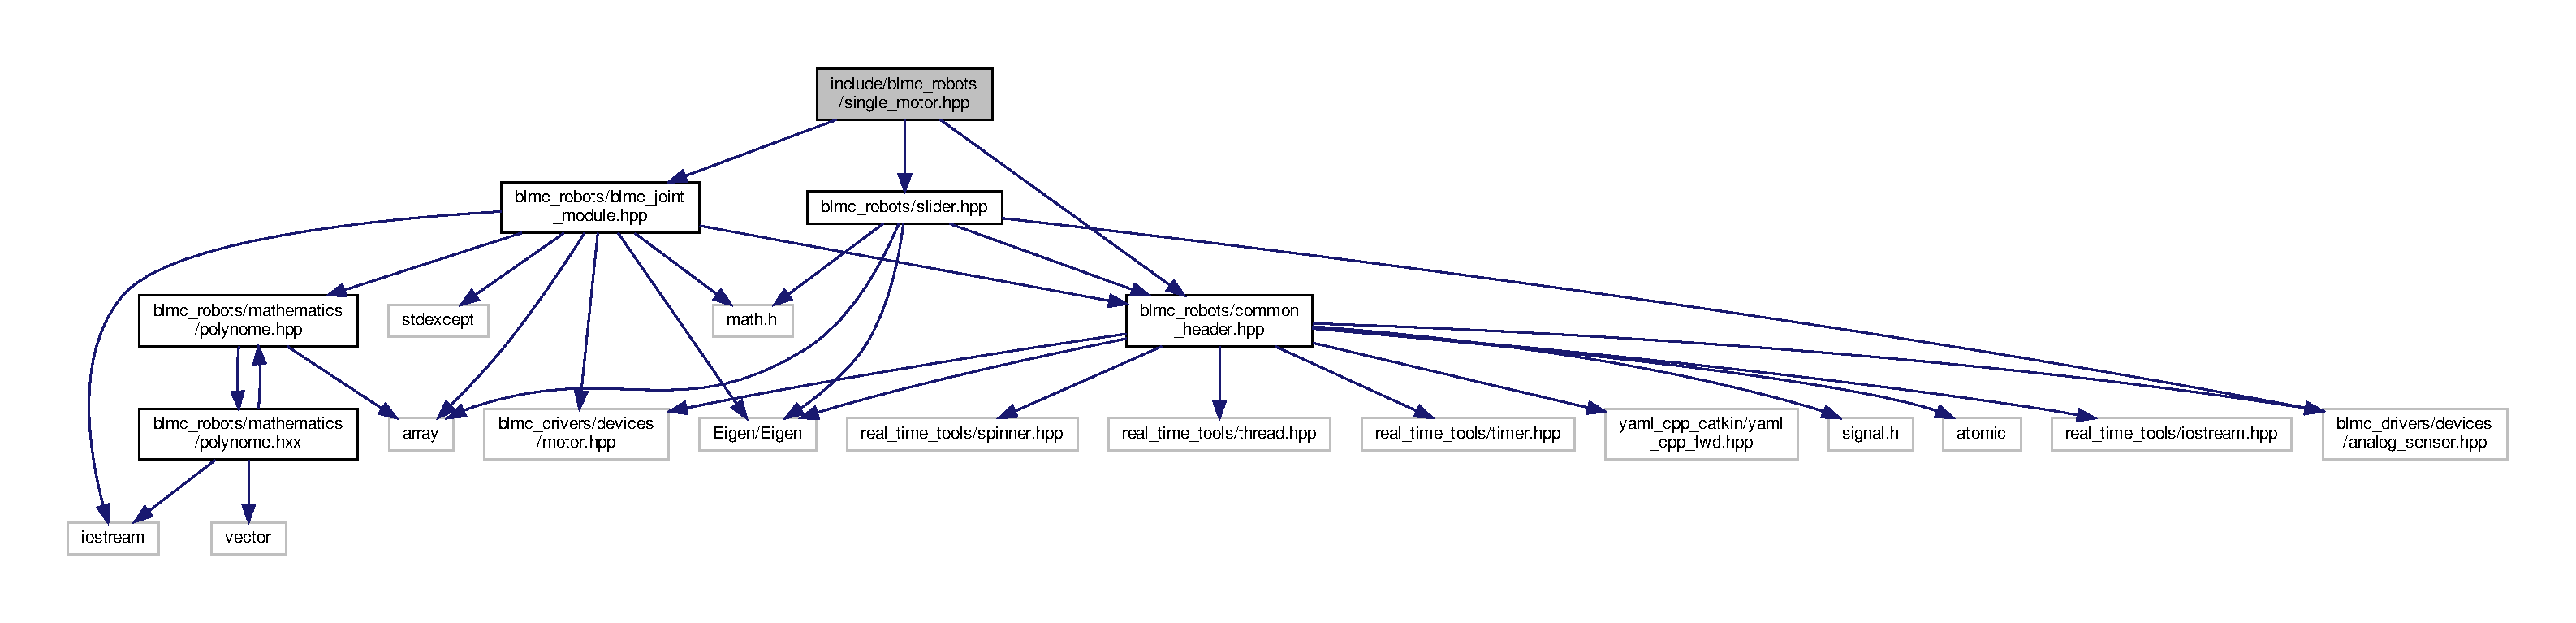
\includegraphics[width=350pt]{single__motor_8hpp__incl}
\end{center}
\end{figure}
\subsection*{Classes}
\begin{DoxyCompactItemize}
\item 
class \hyperlink{classblmc__robots_1_1SingleMotor}{blmc\+\_\+robots\+::\+Single\+Motor}
\end{DoxyCompactItemize}


\subsection{Detailed Description}
\begin{DoxyAuthor}{Author}
Manuel Wuthrich 
\end{DoxyAuthor}
\begin{DoxyDate}{Date}
2018 
\end{DoxyDate}
\begin{DoxyCopyright}{Copyright}
Copyright (c) 2019, New York University \& Max Planck Gesellschaft. 
\end{DoxyCopyright}

\hypertarget{slider_8hpp}{}\section{include/blmc\+\_\+robots/slider.hpp File Reference}
\label{slider_8hpp}\index{include/blmc\+\_\+robots/slider.\+hpp@{include/blmc\+\_\+robots/slider.\+hpp}}
{\ttfamily \#include $<$array$>$}\newline
{\ttfamily \#include $<$math.\+h$>$}\newline
{\ttfamily \#include $<$Eigen/\+Eigen$>$}\newline
{\ttfamily \#include $<$blmc\+\_\+drivers/devices/analog\+\_\+sensor.\+hpp$>$}\newline
{\ttfamily \#include $<$blmc\+\_\+robots/common\+\_\+header.\+hpp$>$}\newline
Include dependency graph for slider.\+hpp\+:
\nopagebreak
\begin{figure}[H]
\begin{center}
\leavevmode
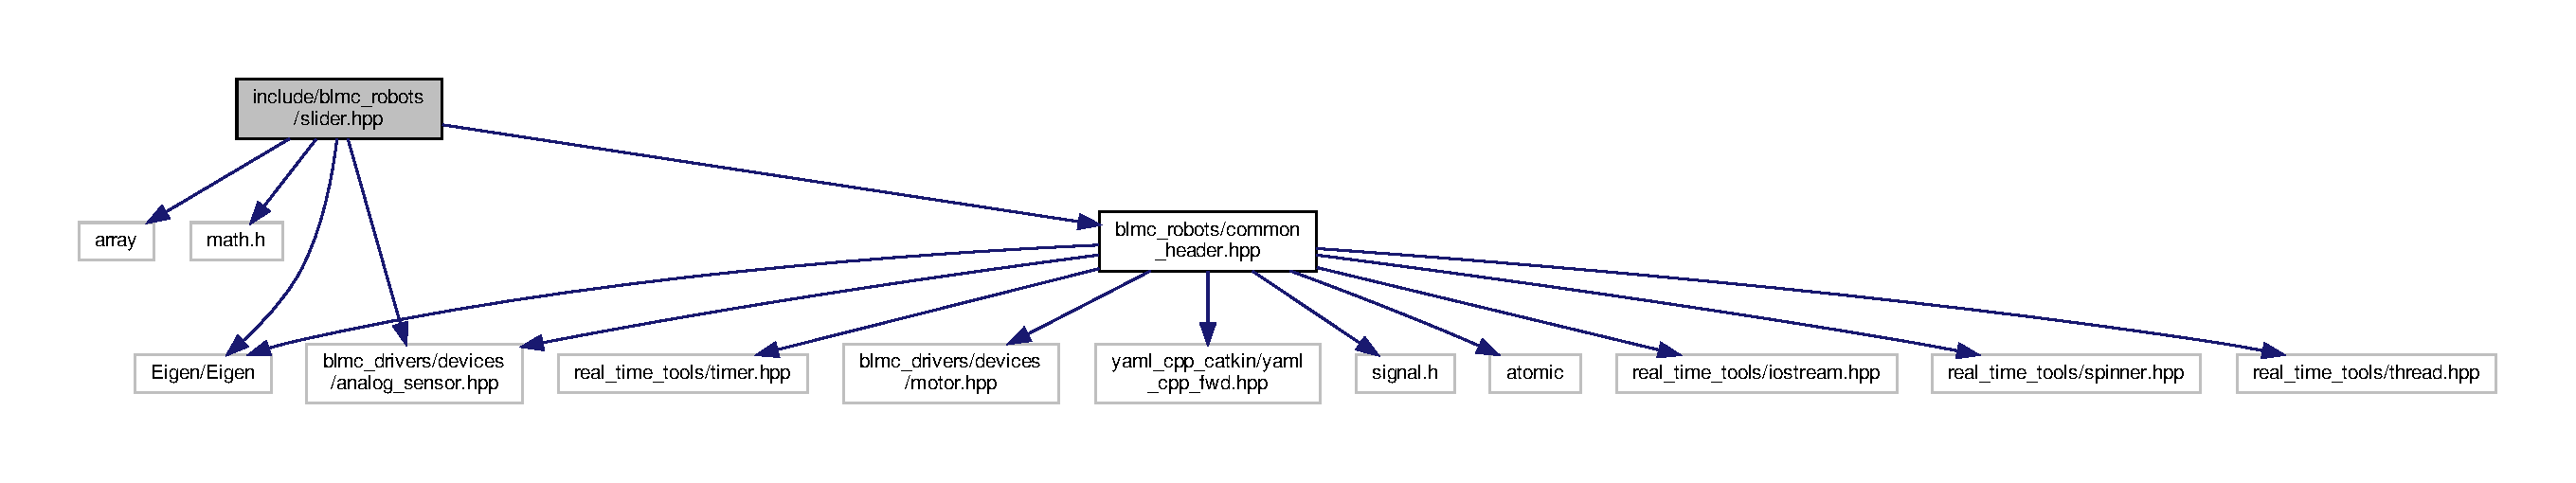
\includegraphics[width=350pt]{slider_8hpp__incl}
\end{center}
\end{figure}
This graph shows which files directly or indirectly include this file\+:
\nopagebreak
\begin{figure}[H]
\begin{center}
\leavevmode
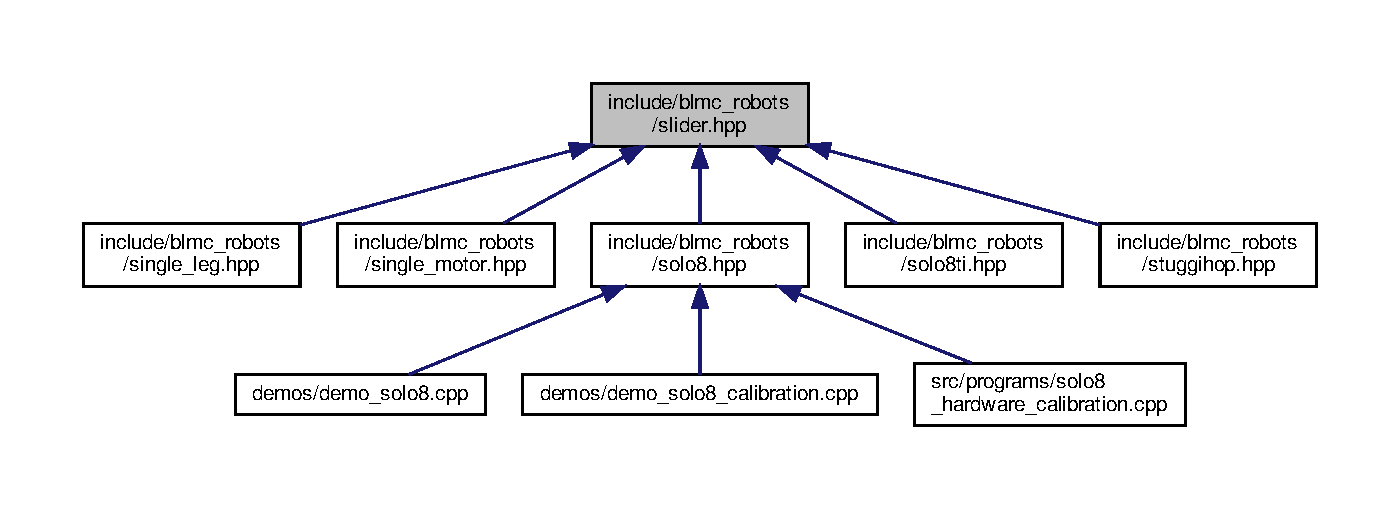
\includegraphics[width=350pt]{slider_8hpp__dep__incl}
\end{center}
\end{figure}
\subsection*{Classes}
\begin{DoxyCompactItemize}
\item 
class \hyperlink{classblmc__robots_1_1Slider}{blmc\+\_\+robots\+::\+Slider}
\item 
class \hyperlink{classblmc__robots_1_1Sliders}{blmc\+\_\+robots\+::\+Sliders$<$ C\+O\+U\+N\+T $>$}
\end{DoxyCompactItemize}


\subsection{Detailed Description}
\begin{DoxyAuthor}{Author}
Manuel Wuthrich 
\end{DoxyAuthor}
\begin{DoxyDate}{Date}
2018 
\end{DoxyDate}
\begin{DoxyCopyright}{Copyright}
Copyright (c) 2019, New York University \& Max Planck Gesellschaft. 
\end{DoxyCopyright}

\hypertarget{solo12_8hpp}{}\section{include/blmc\+\_\+robots/solo12.hpp File Reference}
\label{solo12_8hpp}\index{include/blmc\+\_\+robots/solo12.\+hpp@{include/blmc\+\_\+robots/solo12.\+hpp}}
{\ttfamily \#include $<$blmc\+\_\+drivers/devices/spi\+\_\+motor\+\_\+board.\+hpp$>$}\newline
{\ttfamily \#include \char`\"{}blmc\+\_\+robots/common\+\_\+header.\+hpp\char`\"{}}\newline
{\ttfamily \#include \char`\"{}blmc\+\_\+drivers/serial\+\_\+reader.\+hpp\char`\"{}}\newline
{\ttfamily \#include \char`\"{}blmc\+\_\+robots/blmc\+\_\+joint\+\_\+module.\+hpp\char`\"{}}\newline
Include dependency graph for solo12.\+hpp\+:
\nopagebreak
\begin{figure}[H]
\begin{center}
\leavevmode
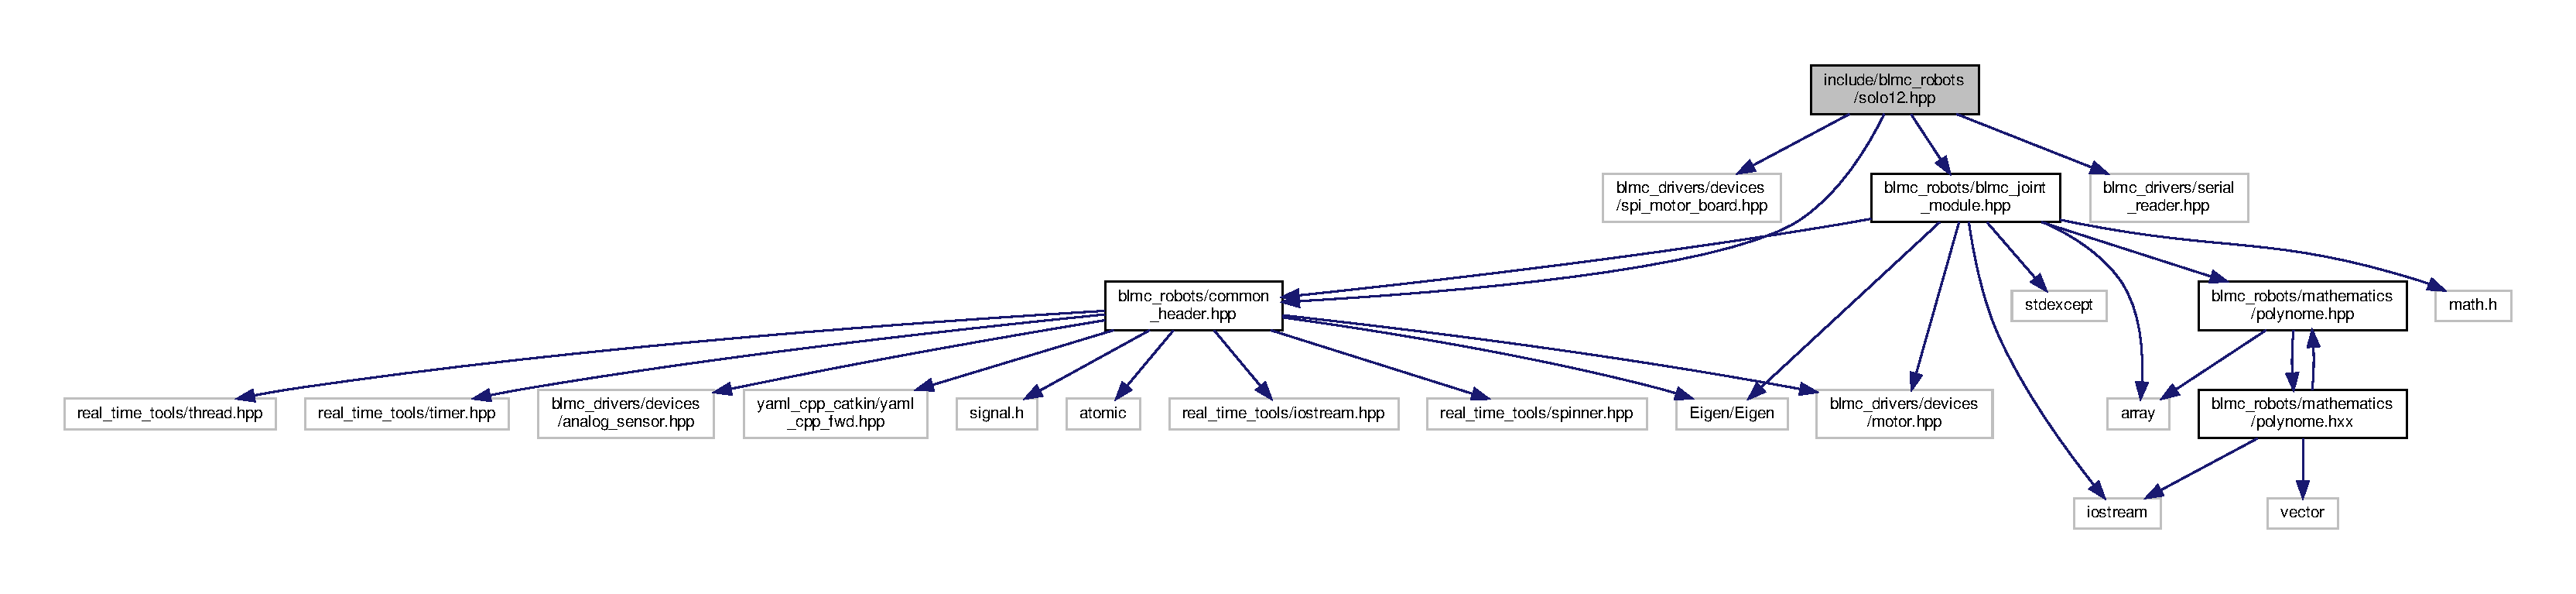
\includegraphics[width=350pt]{solo12_8hpp__incl}
\end{center}
\end{figure}
This graph shows which files directly or indirectly include this file\+:
\nopagebreak
\begin{figure}[H]
\begin{center}
\leavevmode
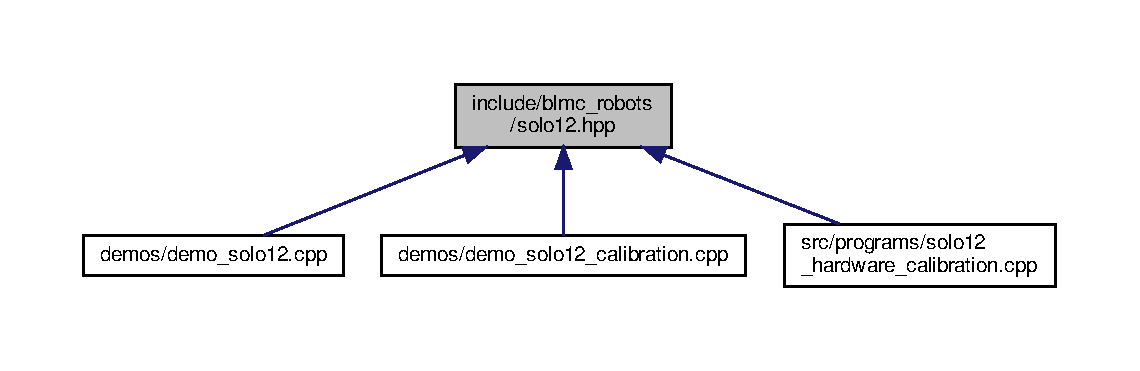
\includegraphics[width=350pt]{solo12_8hpp__dep__incl}
\end{center}
\end{figure}
\subsection*{Classes}
\begin{DoxyCompactItemize}
\item 
class \hyperlink{classblmc__robots_1_1Solo12}{blmc\+\_\+robots\+::\+Solo12}
\begin{DoxyCompactList}\small\item\em Definition and drivers for the \hyperlink{classblmc__robots_1_1Solo12}{Solo12} robot. \end{DoxyCompactList}\end{DoxyCompactItemize}


\subsection{Detailed Description}
\begin{DoxyAuthor}{Author}
Julian Viereck 
\end{DoxyAuthor}
\begin{DoxyDate}{Date}
21 November 2019 
\end{DoxyDate}
\begin{DoxyCopyright}{Copyright}
Copyright (c) 2019, New York University and Max Planck Gesellschaft. 
\end{DoxyCopyright}

\hypertarget{solo8_8hpp}{}\section{include/blmc\+\_\+robots/solo8.hpp File Reference}
\label{solo8_8hpp}\index{include/blmc\+\_\+robots/solo8.\+hpp@{include/blmc\+\_\+robots/solo8.\+hpp}}


Solo8 robot with micro drivers.  


{\ttfamily \#include $<$blmc\+\_\+drivers/serial\+\_\+reader.\+hpp$>$}\newline
{\ttfamily \#include $<$blmc\+\_\+robots/common\+\_\+header.\+hpp$>$}\newline
{\ttfamily \#include $<$blmc\+\_\+robots/slider.\+hpp$>$}\newline
{\ttfamily \#include $<$blmc\+\_\+robots/spi\+\_\+joint\+\_\+module.\+hpp$>$}\newline
Include dependency graph for solo8.\+hpp\+:
\nopagebreak
\begin{figure}[H]
\begin{center}
\leavevmode
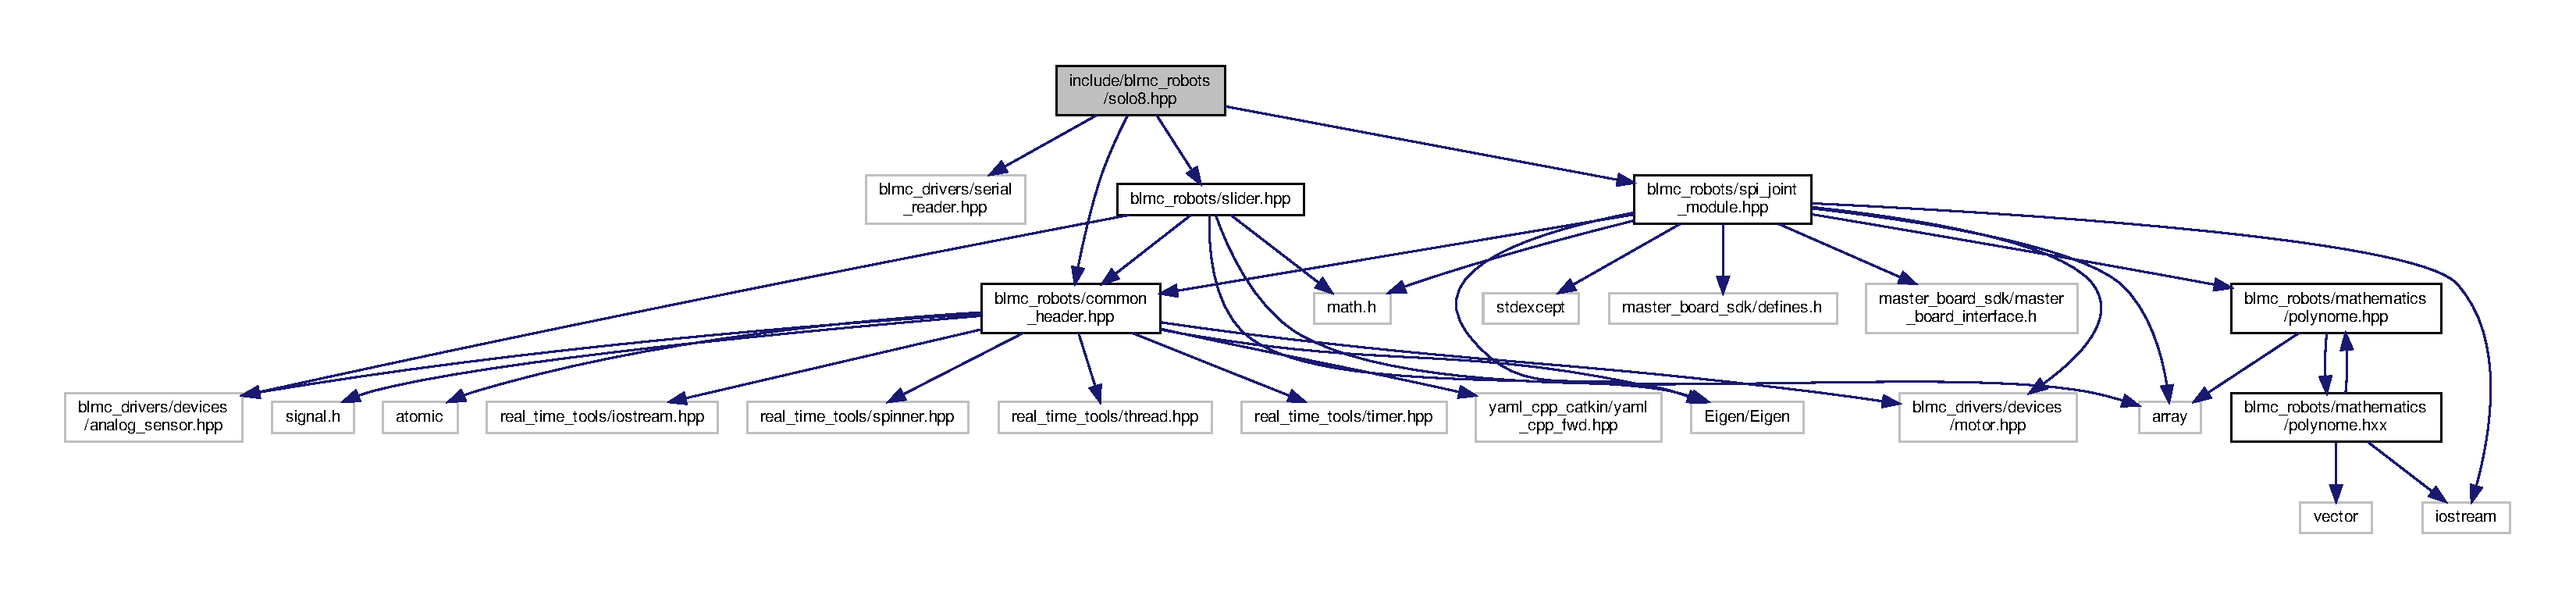
\includegraphics[width=350pt]{solo8_8hpp__incl}
\end{center}
\end{figure}
This graph shows which files directly or indirectly include this file\+:
\nopagebreak
\begin{figure}[H]
\begin{center}
\leavevmode
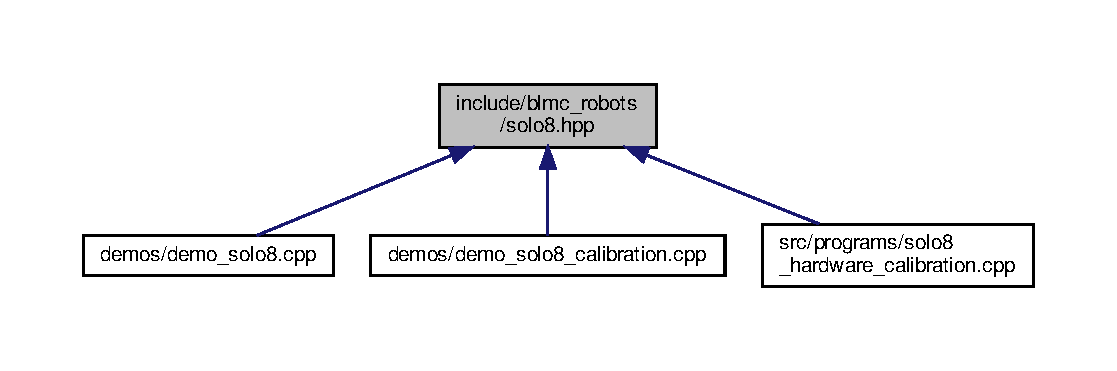
\includegraphics[width=350pt]{solo8_8hpp__dep__incl}
\end{center}
\end{figure}
\subsection*{Classes}
\begin{DoxyCompactItemize}
\item 
class \hyperlink{classblmc__robots_1_1Solo8}{blmc\+\_\+robots\+::\+Solo8}
\end{DoxyCompactItemize}


\subsection{Detailed Description}
Solo8 robot with micro drivers. 

\begin{DoxyAuthor}{Author}
Julian Viereck 
\end{DoxyAuthor}
\begin{DoxyDate}{Date}
2020 
\end{DoxyDate}
\begin{DoxyCopyright}{Copyright}
Copyright (c) 2020, New York University \& Max Planck Gesellschaft. 
\end{DoxyCopyright}

\hypertarget{stuggihop_8hpp}{}\section{include/blmc\+\_\+robots/stuggihop.hpp File Reference}
\label{stuggihop_8hpp}\index{include/blmc\+\_\+robots/stuggihop.\+hpp@{include/blmc\+\_\+robots/stuggihop.\+hpp}}
{\ttfamily \#include $<$blmc\+\_\+robots/blmc\+\_\+joint\+\_\+module.\+hpp$>$}\newline
{\ttfamily \#include $<$blmc\+\_\+robots/common\+\_\+header.\+hpp$>$}\newline
{\ttfamily \#include $<$blmc\+\_\+robots/slider.\+hpp$>$}\newline
Include dependency graph for stuggihop.\+hpp\+:
\nopagebreak
\begin{figure}[H]
\begin{center}
\leavevmode
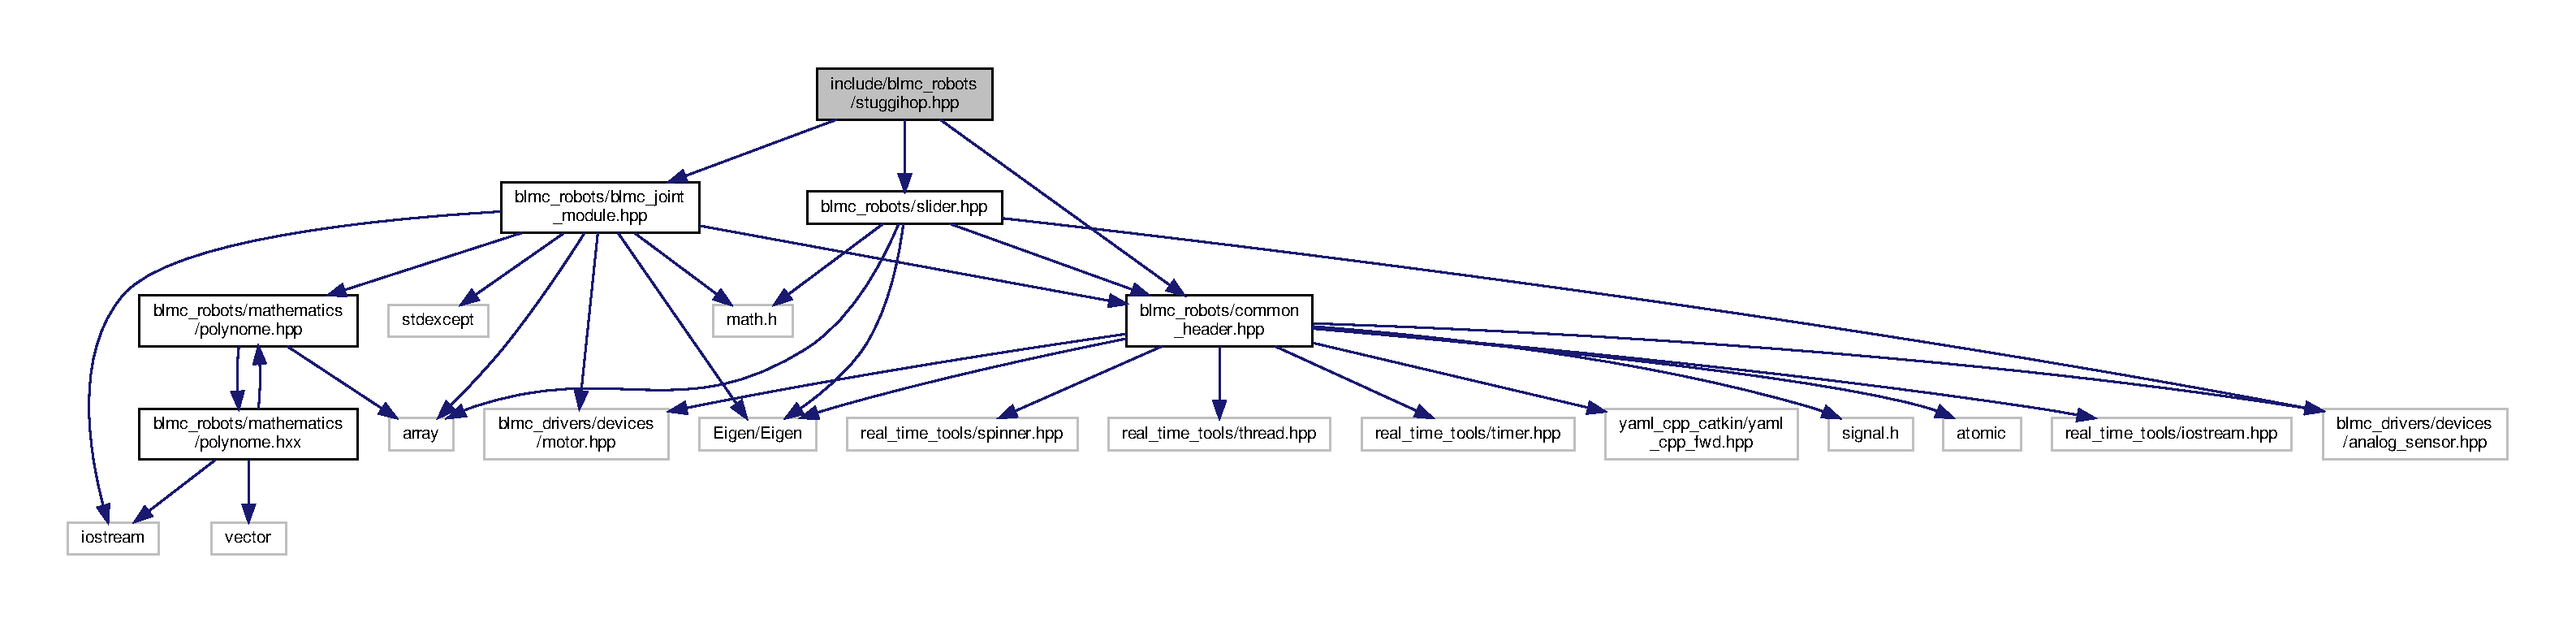
\includegraphics[width=350pt]{stuggihop_8hpp__incl}
\end{center}
\end{figure}
\subsection*{Classes}
\begin{DoxyCompactItemize}
\item 
class \hyperlink{classblmc__robots_1_1Stuggihop}{blmc\+\_\+robots\+::\+Stuggihop}
\end{DoxyCompactItemize}


\subsection{Detailed Description}
\begin{DoxyAuthor}{Author}
Manuel Wuthrich 
\end{DoxyAuthor}
\begin{DoxyDate}{Date}
2018 
\end{DoxyDate}
\begin{DoxyCopyright}{Copyright}
Copyright (c) 2019, New York University \& Max Planck Gesellschaft. 
\end{DoxyCopyright}

\hypertarget{test__bench__8__motors_8hpp}{}\section{include/blmc\+\_\+robots/test\+\_\+bench\+\_\+8\+\_\+motors.hpp File Reference}
\label{test__bench__8__motors_8hpp}\index{include/blmc\+\_\+robots/test\+\_\+bench\+\_\+8\+\_\+motors.\+hpp@{include/blmc\+\_\+robots/test\+\_\+bench\+\_\+8\+\_\+motors.\+hpp}}


The hardware wrapper of the test bench with 8 blmc motors.  


{\ttfamily \#include $<$blmc\+\_\+robots/common\+\_\+header.\+hpp$>$}\newline
Include dependency graph for test\+\_\+bench\+\_\+8\+\_\+motors.\+hpp\+:
\nopagebreak
\begin{figure}[H]
\begin{center}
\leavevmode
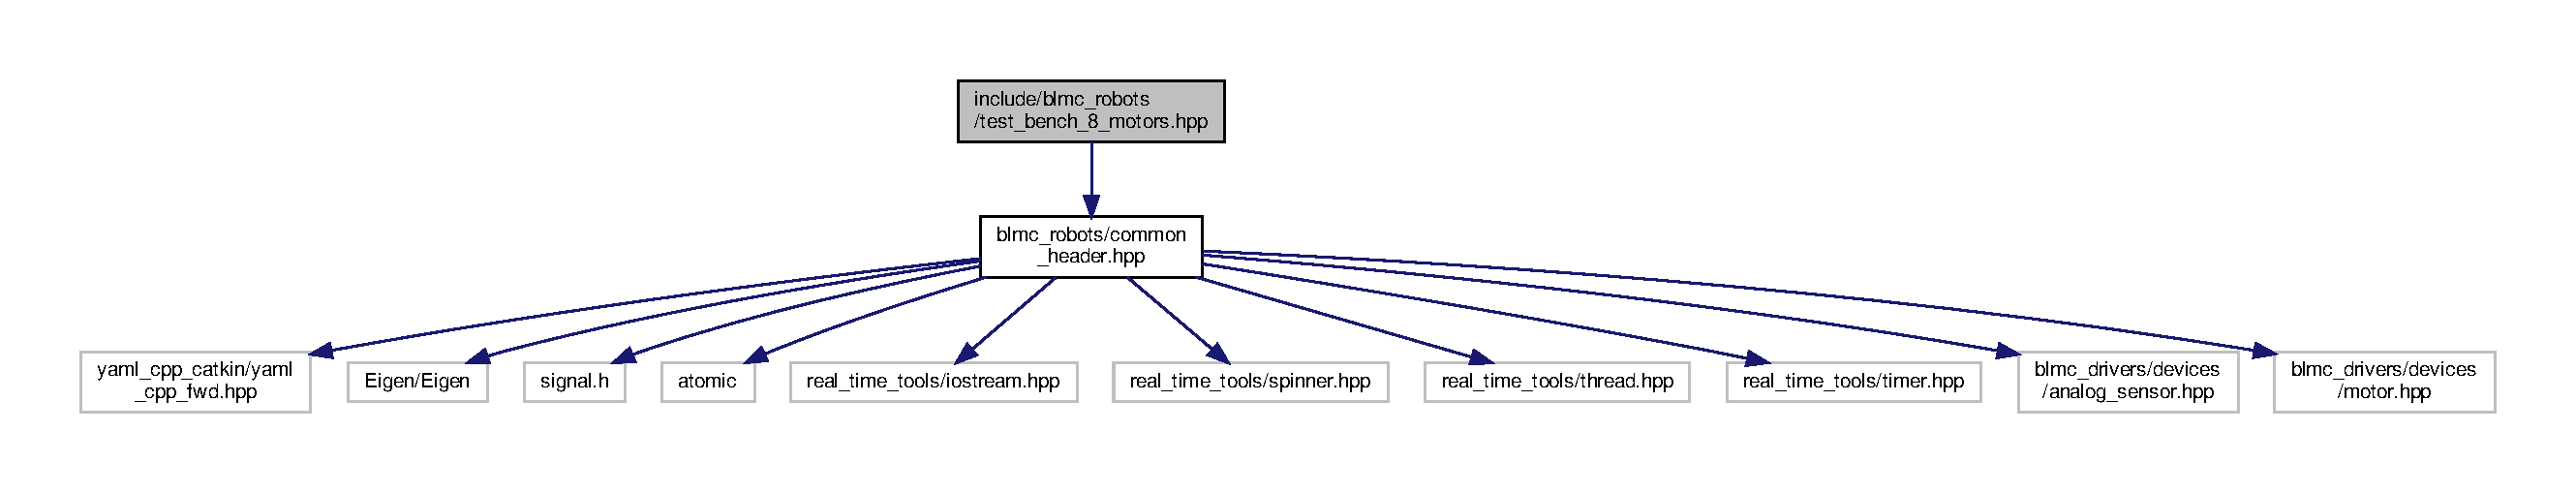
\includegraphics[width=350pt]{test__bench__8__motors_8hpp__incl}
\end{center}
\end{figure}
This graph shows which files directly or indirectly include this file\+:
\nopagebreak
\begin{figure}[H]
\begin{center}
\leavevmode
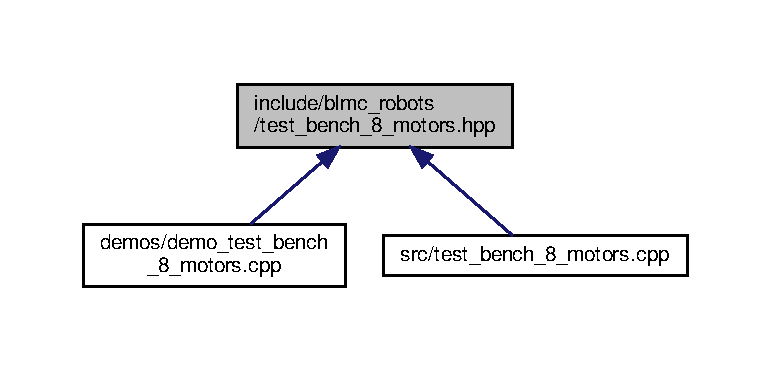
\includegraphics[width=350pt]{test__bench__8__motors_8hpp__dep__incl}
\end{center}
\end{figure}
\subsection*{Classes}
\begin{DoxyCompactItemize}
\item 
class \hyperlink{classblmc__robots_1_1TestBench8Motors}{blmc\+\_\+robots\+::\+Test\+Bench8\+Motors}
\begin{DoxyCompactList}\small\item\em The \hyperlink{classblmc__robots_1_1TestBench8Motors}{Test\+Bench8\+Motors} class implements the control of the test bench containing 8 motors and 8 sliders using the blmc drivers. \end{DoxyCompactList}\end{DoxyCompactItemize}


\subsection{Detailed Description}
The hardware wrapper of the test bench with 8 blmc motors. 

\begin{DoxyAuthor}{Author}
Maximilien Naveau 
\end{DoxyAuthor}
\begin{DoxyDate}{Date}
2018
\end{DoxyDate}
This file declares the Test\+Bench8\+Motors class which defines the test bench with 8 motors. 
\hypertarget{teststand_8hpp}{}\section{include/blmc\+\_\+robots/teststand.hpp File Reference}
\label{teststand_8hpp}\index{include/blmc\+\_\+robots/teststand.\+hpp@{include/blmc\+\_\+robots/teststand.\+hpp}}
{\ttfamily \#include $<$Ati\+F\+T\+Sensor.\+h$>$}\newline
{\ttfamily \#include $<$blmc\+\_\+robots/blmc\+\_\+joint\+\_\+module.\+hpp$>$}\newline
{\ttfamily \#include $<$blmc\+\_\+robots/common\+\_\+header.\+hpp$>$}\newline
Include dependency graph for teststand.\+hpp\+:
\nopagebreak
\begin{figure}[H]
\begin{center}
\leavevmode
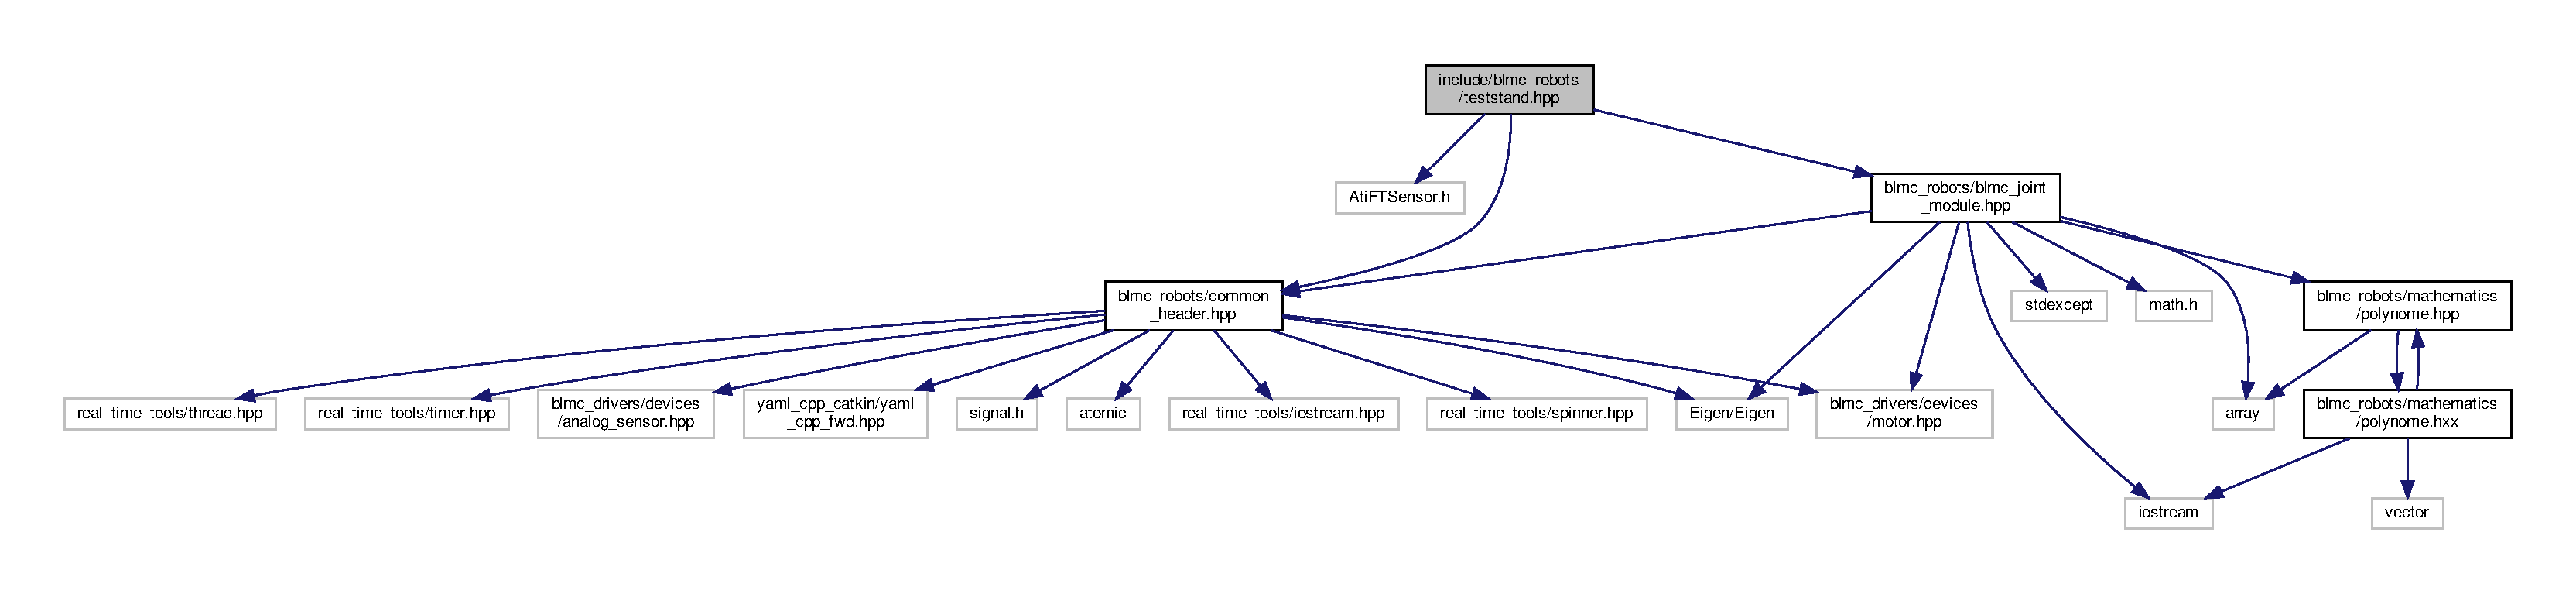
\includegraphics[width=350pt]{teststand_8hpp__incl}
\end{center}
\end{figure}
This graph shows which files directly or indirectly include this file\+:
\nopagebreak
\begin{figure}[H]
\begin{center}
\leavevmode
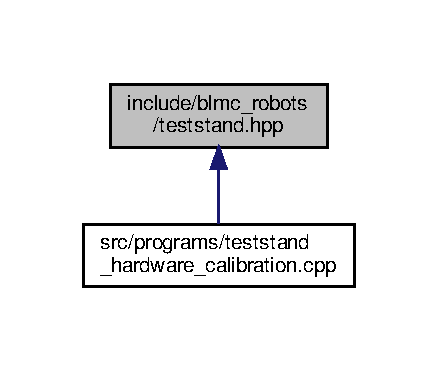
\includegraphics[width=210pt]{teststand_8hpp__dep__incl}
\end{center}
\end{figure}
\subsection*{Classes}
\begin{DoxyCompactItemize}
\item 
class \hyperlink{classblmc__robots_1_1Teststand}{blmc\+\_\+robots\+::\+Teststand}
\begin{DoxyCompactList}\small\item\em The class \hyperlink{classblmc__robots_1_1Teststand}{Teststand} is used to control the \hyperlink{classblmc__robots_1_1Teststand}{Teststand} robot located at M\+P\+I-\/\+IS Tuebingen. \end{DoxyCompactList}\end{DoxyCompactItemize}


\subsection{Detailed Description}
\begin{DoxyAuthor}{Author}
Manuel Wuthrich 
\end{DoxyAuthor}
\begin{DoxyDate}{Date}
2018 
\end{DoxyDate}
\begin{DoxyCopyright}{Copyright}
Copyright (c) 2019, New York University \& Max Planck Gesellschaft. 
\end{DoxyCopyright}

\hypertarget{blmc__joint__module_8cpp}{}\section{src/blmc\+\_\+joint\+\_\+module.cpp File Reference}
\label{blmc__joint__module_8cpp}\index{src/blmc\+\_\+joint\+\_\+module.\+cpp@{src/blmc\+\_\+joint\+\_\+module.\+cpp}}
{\ttfamily \#include \char`\"{}blmc\+\_\+robots/blmc\+\_\+joint\+\_\+module.\+hpp\char`\"{}}\newline
{\ttfamily \#include $<$cmath$>$}\newline
{\ttfamily \#include \char`\"{}real\+\_\+time\+\_\+tools/iostream.\+hpp\char`\"{}}\newline
{\ttfamily \#include \char`\"{}real\+\_\+time\+\_\+tools/spinner.\+hpp\char`\"{}}\newline
Include dependency graph for blmc\+\_\+joint\+\_\+module.\+cpp\+:
\nopagebreak
\begin{figure}[H]
\begin{center}
\leavevmode
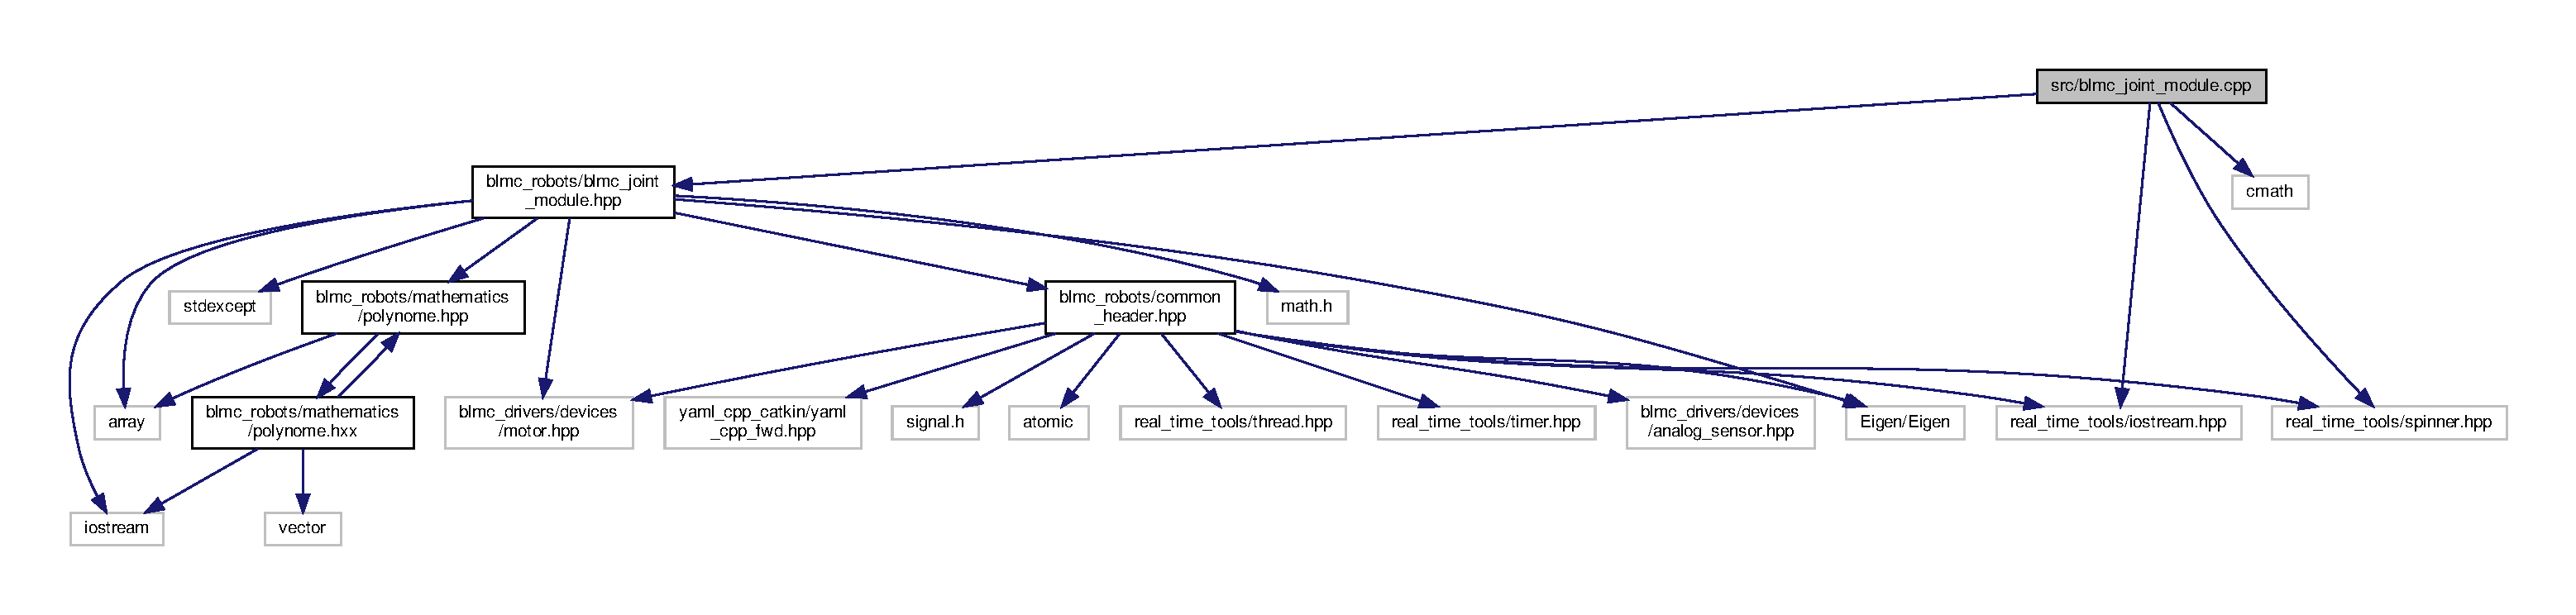
\includegraphics[width=350pt]{blmc__joint__module_8cpp__incl}
\end{center}
\end{figure}


\subsection{Detailed Description}
\begin{DoxyAuthor}{Author}
Maximilien Naveau (\href{mailto:maximilien.naveau@gmail.com}{\tt maximilien.\+naveau@gmail.\+com}) 

Manuel Wuthrich 
\end{DoxyAuthor}
\begin{DoxyRefDesc}{License}
\item[\hyperlink{license__license000003}{License}]License B\+S\+D-\/3-\/\+Clause \end{DoxyRefDesc}
\begin{DoxyCopyright}{Copyright}
Copyright (c) 2019, New York University and Max Planck Gesellschaft. 
\end{DoxyCopyright}
\begin{DoxyDate}{Date}
2019-\/07-\/11 
\end{DoxyDate}

\hypertarget{polynome_8cpp}{}\section{src/mathematics/polynome.cpp File Reference}
\label{polynome_8cpp}\index{src/mathematics/polynome.\+cpp@{src/mathematics/polynome.\+cpp}}


Polynomes object for trajectories.  


{\ttfamily \#include $<$blmc\+\_\+robots/mathematics/polynome.\+hpp$>$}\newline
{\ttfamily \#include $<$iostream$>$}\newline
Include dependency graph for polynome.\+cpp\+:
\nopagebreak
\begin{figure}[H]
\begin{center}
\leavevmode
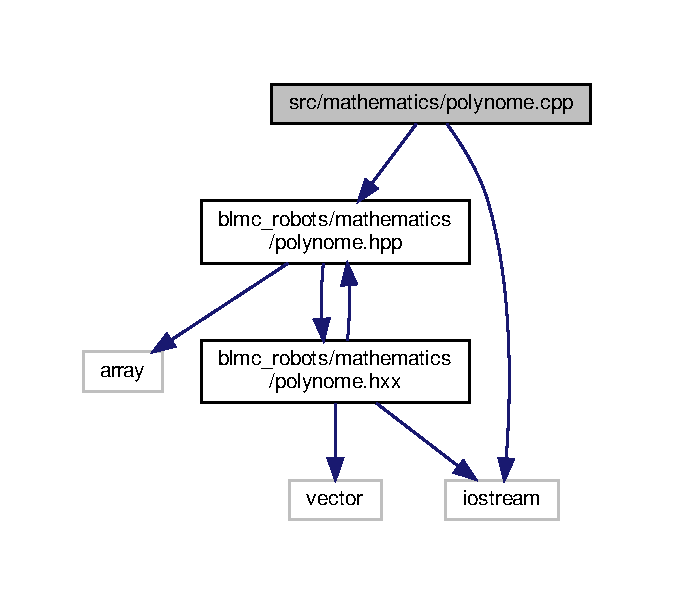
\includegraphics[width=324pt]{polynome_8cpp__incl}
\end{center}
\end{figure}


\subsection{Detailed Description}
Polynomes object for trajectories. 

\begin{DoxyAuthor}{Author}
Maximilien Naveau (\href{mailto:maximilien.naveau@gmail.com}{\tt maximilien.\+naveau@gmail.\+com}) 
\end{DoxyAuthor}
\begin{DoxyVersion}{Version}
0.\+1 
\end{DoxyVersion}
\begin{DoxyDate}{Date}
2019-\/11-\/07
\end{DoxyDate}
\begin{DoxyCopyright}{Copyright}
Copyright (c) 2019
\end{DoxyCopyright}
See \href{https://github.com/jrl-umi3218/jrl-walkgen/blob/master/src/Mathematics/PolynomeFoot.cpp}{\tt https\+://github.\+com/jrl-\/umi3218/jrl-\/walkgen/blob/master/src/\+Mathematics/\+Polynome\+Foot.\+cpp} for further enhancement. 
\hypertarget{solo12__hardware__calibration_8cpp}{}\section{src/programs/solo12\+\_\+hardware\+\_\+calibration.cpp File Reference}
\label{solo12__hardware__calibration_8cpp}\index{src/programs/solo12\+\_\+hardware\+\_\+calibration.\+cpp@{src/programs/solo12\+\_\+hardware\+\_\+calibration.\+cpp}}


...  


{\ttfamily \#include \char`\"{}blmc\+\_\+robots/common\+\_\+programs\+\_\+header.\+hpp\char`\"{}}\newline
{\ttfamily \#include \char`\"{}blmc\+\_\+robots/solo12.\+hpp\char`\"{}}\newline
Include dependency graph for solo12\+\_\+hardware\+\_\+calibration.\+cpp\+:
\nopagebreak
\begin{figure}[H]
\begin{center}
\leavevmode
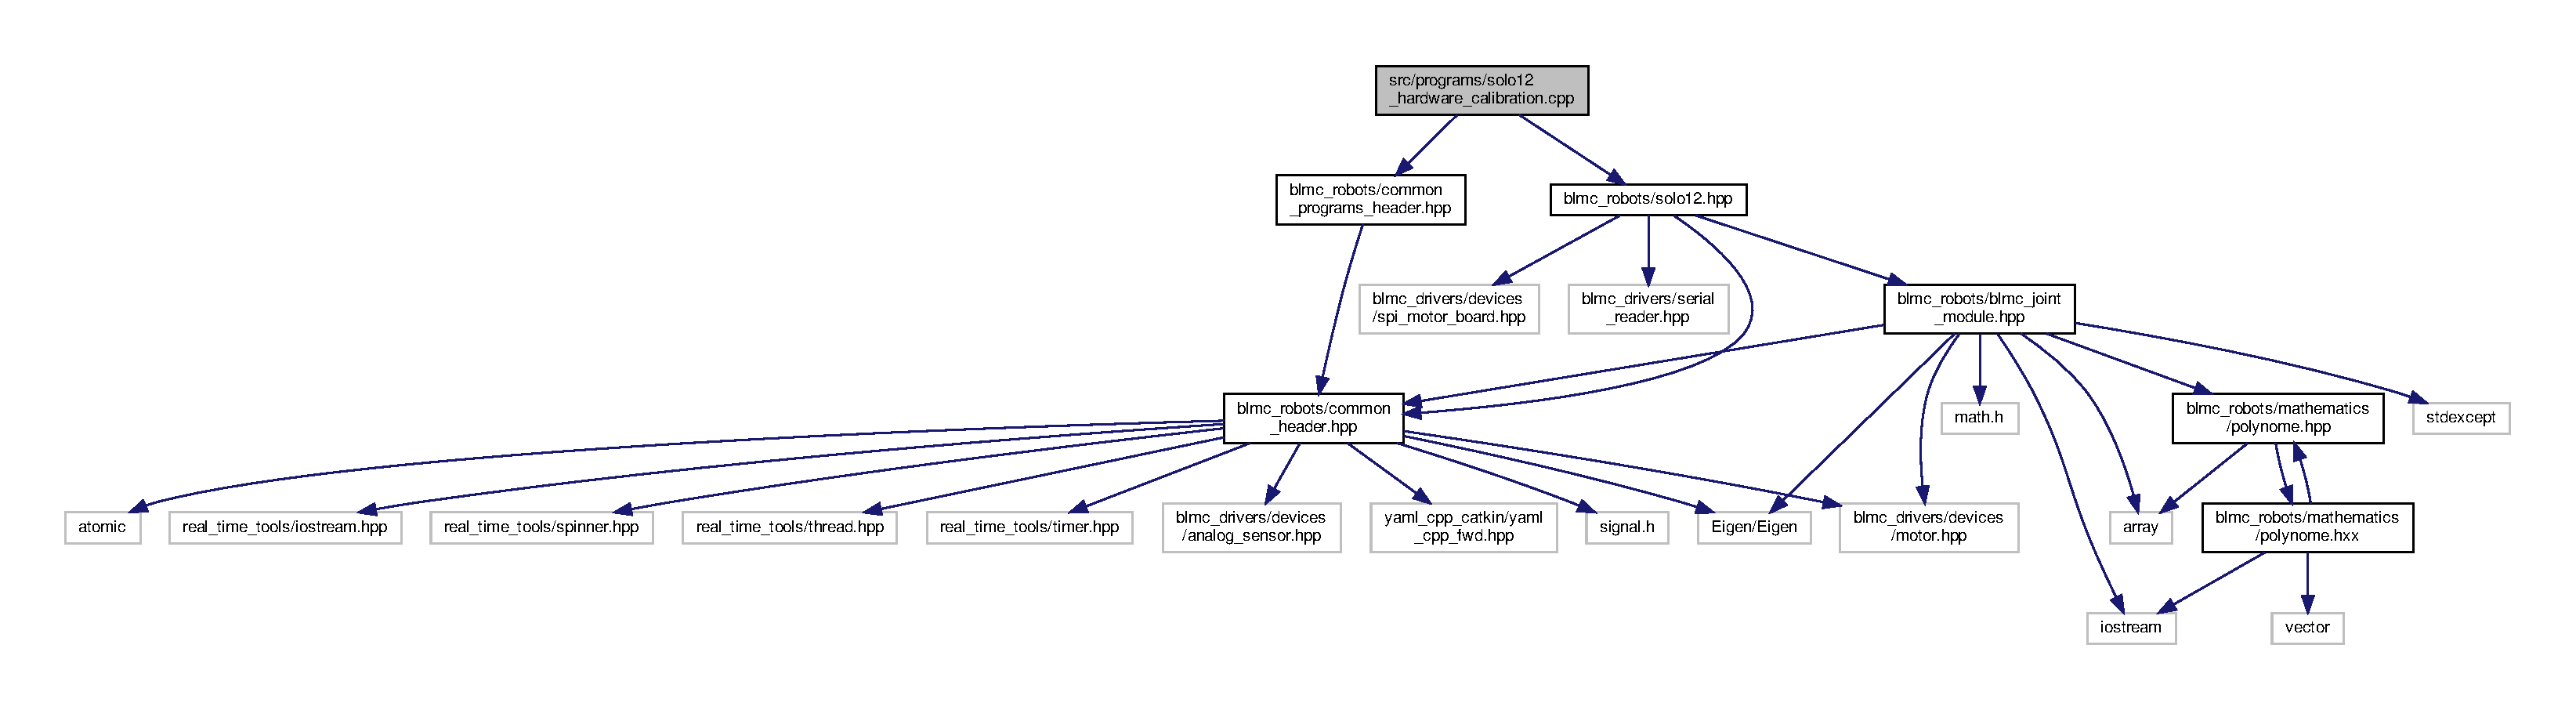
\includegraphics[width=350pt]{solo12__hardware__calibration_8cpp__incl}
\end{center}
\end{figure}
\subsection*{Functions}
\begin{DoxyCompactItemize}
\item 
\mbox{\Hypertarget{solo12__hardware__calibration_8cpp_a39957cbbba118d0d10bbc093b6b1ff5a}\label{solo12__hardware__calibration_8cpp_a39957cbbba118d0d10bbc093b6b1ff5a}} 
static T\+H\+R\+E\+A\+D\+\_\+\+F\+U\+N\+C\+T\+I\+O\+N\+\_\+\+R\+E\+T\+U\+R\+N\+\_\+\+T\+Y\+PE {\bfseries control\+\_\+loop} (void $\ast$robot\+\_\+void\+\_\+ptr)
\item 
\mbox{\Hypertarget{solo12__hardware__calibration_8cpp_a3c04138a5bfe5d72780bb7e82a18e627}\label{solo12__hardware__calibration_8cpp_a3c04138a5bfe5d72780bb7e82a18e627}} 
int {\bfseries main} (int argc, char $\ast$$\ast$argv)
\end{DoxyCompactItemize}


\subsection{Detailed Description}
... 

\begin{DoxyAuthor}{Author}
Maximilien Naveau 
\end{DoxyAuthor}
\begin{DoxyDate}{Date}
2018
\end{DoxyDate}
This file uses the Solo12 class in a small demo. 
\hypertarget{solo8__hardware__calibration_8cpp}{}\section{src/programs/solo8\+\_\+hardware\+\_\+calibration.cpp File Reference}
\label{solo8__hardware__calibration_8cpp}\index{src/programs/solo8\+\_\+hardware\+\_\+calibration.\+cpp@{src/programs/solo8\+\_\+hardware\+\_\+calibration.\+cpp}}


...  


{\ttfamily \#include \char`\"{}blmc\+\_\+robots/common\+\_\+programs\+\_\+header.\+hpp\char`\"{}}\newline
{\ttfamily \#include \char`\"{}blmc\+\_\+robots/solo8.\+hpp\char`\"{}}\newline
Include dependency graph for solo8\+\_\+hardware\+\_\+calibration.\+cpp\+:
\nopagebreak
\begin{figure}[H]
\begin{center}
\leavevmode
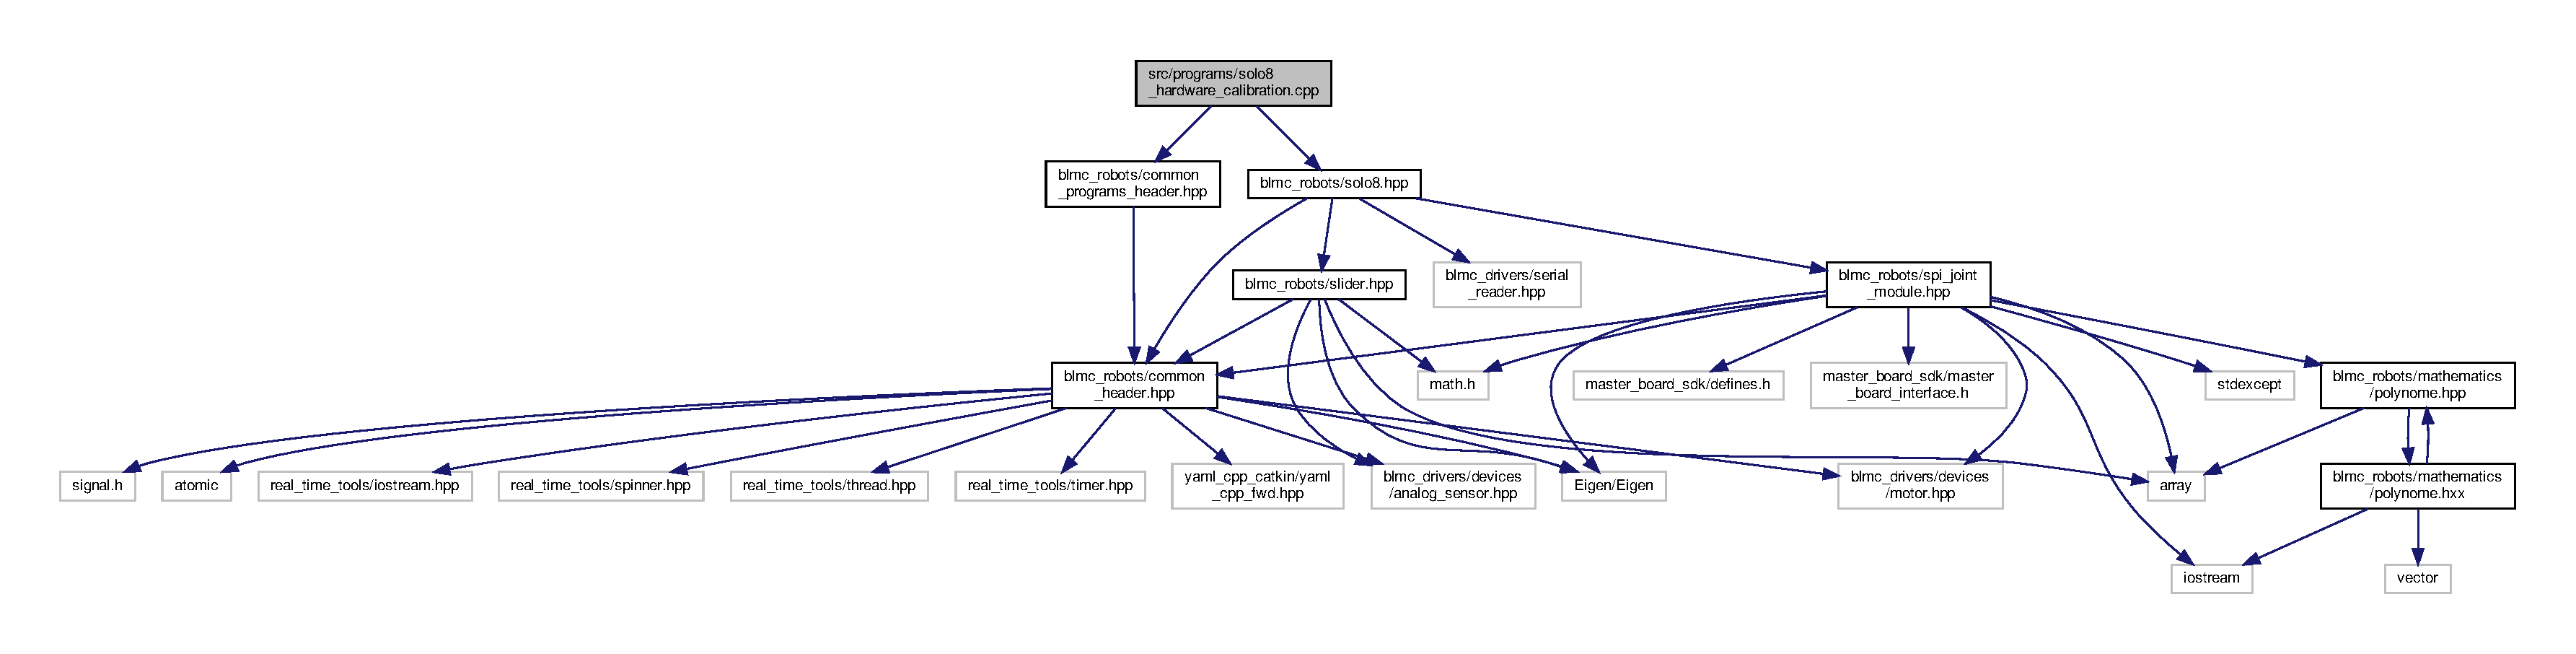
\includegraphics[width=350pt]{solo8__hardware__calibration_8cpp__incl}
\end{center}
\end{figure}
\subsection*{Functions}
\begin{DoxyCompactItemize}
\item 
\mbox{\Hypertarget{solo8__hardware__calibration_8cpp_a39957cbbba118d0d10bbc093b6b1ff5a}\label{solo8__hardware__calibration_8cpp_a39957cbbba118d0d10bbc093b6b1ff5a}} 
static T\+H\+R\+E\+A\+D\+\_\+\+F\+U\+N\+C\+T\+I\+O\+N\+\_\+\+R\+E\+T\+U\+R\+N\+\_\+\+T\+Y\+PE {\bfseries control\+\_\+loop} (void $\ast$robot\+\_\+void\+\_\+ptr)
\item 
\mbox{\Hypertarget{solo8__hardware__calibration_8cpp_a3c04138a5bfe5d72780bb7e82a18e627}\label{solo8__hardware__calibration_8cpp_a3c04138a5bfe5d72780bb7e82a18e627}} 
int {\bfseries main} (int argc, char $\ast$$\ast$argv)
\end{DoxyCompactItemize}


\subsection{Detailed Description}
... 

\begin{DoxyAuthor}{Author}
Maximilien Naveau 
\end{DoxyAuthor}
\begin{DoxyDate}{Date}
2018
\end{DoxyDate}
This file uses the Solo8 class in a small demo. 
\hypertarget{teststand__hardware__calibration_8cpp}{}\section{src/programs/teststand\+\_\+hardware\+\_\+calibration.cpp File Reference}
\label{teststand__hardware__calibration_8cpp}\index{src/programs/teststand\+\_\+hardware\+\_\+calibration.\+cpp@{src/programs/teststand\+\_\+hardware\+\_\+calibration.\+cpp}}


Program that launch the calibration of the testand with 0 offset.  


{\ttfamily \#include \char`\"{}blmc\+\_\+robots/common\+\_\+programs\+\_\+header.\+hpp\char`\"{}}\newline
{\ttfamily \#include \char`\"{}blmc\+\_\+robots/teststand.\+hpp\char`\"{}}\newline
Include dependency graph for teststand\+\_\+hardware\+\_\+calibration.\+cpp\+:
\nopagebreak
\begin{figure}[H]
\begin{center}
\leavevmode
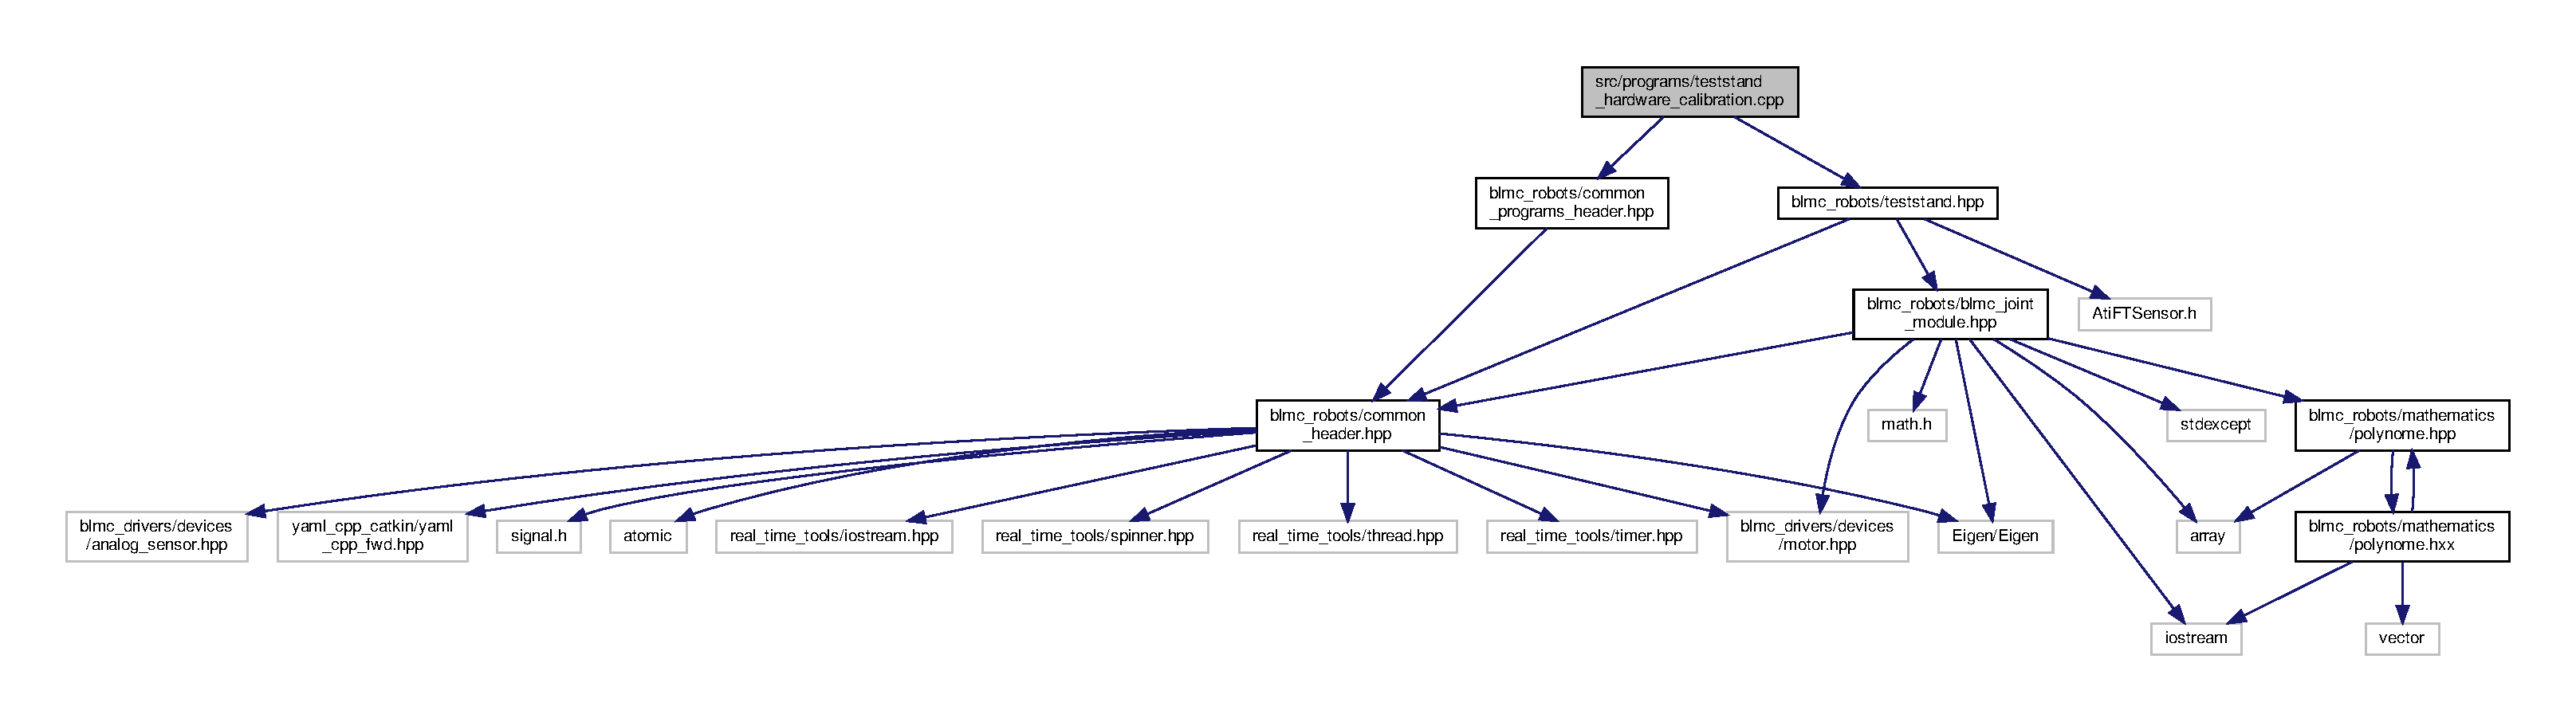
\includegraphics[width=350pt]{teststand__hardware__calibration_8cpp__incl}
\end{center}
\end{figure}
\subsection*{Functions}
\begin{DoxyCompactItemize}
\item 
\mbox{\Hypertarget{teststand__hardware__calibration_8cpp_a39957cbbba118d0d10bbc093b6b1ff5a}\label{teststand__hardware__calibration_8cpp_a39957cbbba118d0d10bbc093b6b1ff5a}} 
static T\+H\+R\+E\+A\+D\+\_\+\+F\+U\+N\+C\+T\+I\+O\+N\+\_\+\+R\+E\+T\+U\+R\+N\+\_\+\+T\+Y\+PE {\bfseries control\+\_\+loop} (void $\ast$robot\+\_\+void\+\_\+ptr)
\item 
\mbox{\Hypertarget{teststand__hardware__calibration_8cpp_a2c3f6775325c30275d11c6abee2db6a0}\label{teststand__hardware__calibration_8cpp_a2c3f6775325c30275d11c6abee2db6a0}} 
int {\bfseries main} (int, char $\ast$$\ast$)
\end{DoxyCompactItemize}


\subsection{Detailed Description}
Program that launch the calibration of the testand with 0 offset. 

\begin{DoxyAuthor}{Author}
Maximilien Naveau (\href{mailto:maximilien.naveau@gmail.com}{\tt maximilien.\+naveau@gmail.\+com}) 
\end{DoxyAuthor}
\begin{DoxyVersion}{Version}
0.\+1 
\end{DoxyVersion}
\begin{DoxyDate}{Date}
2019-\/11-\/08
\end{DoxyDate}
\begin{DoxyCopyright}{Copyright}
Copyright (c) 2019
\end{DoxyCopyright}
This program is a helper for the measurement of the offset between the joint index (home pose) and the theoretical zero defined by the urdf.


\begin{DoxyItemize}
\item It start by initializing the robot.
\item Once done it wait for the user to press enter in order to move the leg to the joint index
\item Then the controller just sends 0 torques and report the current joint pose.
\end{DoxyItemize}

Once this small procedure is done the user can setup the joints in the zero configuration and read the offset in the screen. The offset should be reported at least in the robot\+\_\+properties\+\_\+\mbox{[}robot\+\_\+name\mbox{]}/config/dgm\+\_\+paramter.yaml under the 
\begin{DoxyCode}
hardware\_communication:
  calibration:
     index\_to\_zero\_angle: [...]
\end{DoxyCode}
 
\hypertarget{test__bench__8__motors_8cpp}{}\section{src/test\+\_\+bench\+\_\+8\+\_\+motors.cpp File Reference}
\label{test__bench__8__motors_8cpp}\index{src/test\+\_\+bench\+\_\+8\+\_\+motors.\+cpp@{src/test\+\_\+bench\+\_\+8\+\_\+motors.\+cpp}}


The hardware wrapper of the the test bench with 8 blmc motors.  


{\ttfamily \#include \char`\"{}blmc\+\_\+robots/test\+\_\+bench\+\_\+8\+\_\+motors.\+hpp\char`\"{}}\newline
Include dependency graph for test\+\_\+bench\+\_\+8\+\_\+motors.\+cpp\+:
\nopagebreak
\begin{figure}[H]
\begin{center}
\leavevmode
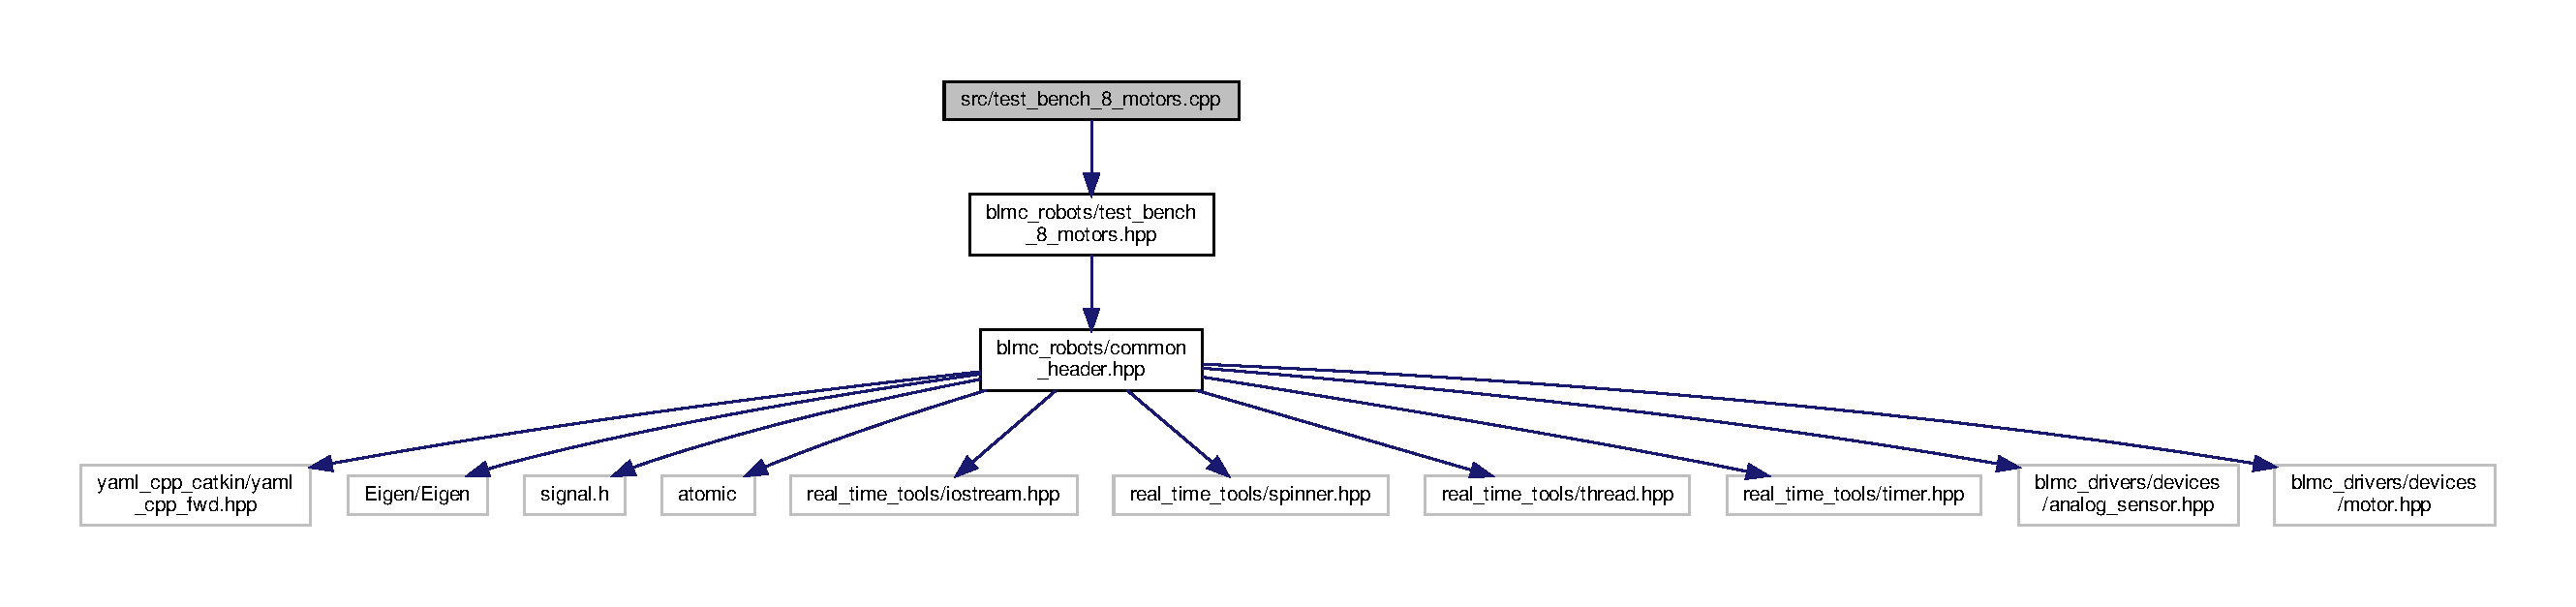
\includegraphics[width=350pt]{test__bench__8__motors_8cpp__incl}
\end{center}
\end{figure}


\subsection{Detailed Description}
The hardware wrapper of the the test bench with 8 blmc motors. 

\begin{DoxyAuthor}{Author}
Maximilien Naveau 
\end{DoxyAuthor}
\begin{DoxyDate}{Date}
2018
\end{DoxyDate}
This file defines the Test\+Bench8\+Motors class. 
\chapter{Example Documentation}
\hypertarget{serial_stream_read_8cpp-example}{}\section{serial\+\_\+stream\+\_\+read.\+cpp}

\begin{DoxyCodeInclude}
\end{DoxyCodeInclude}
 
%--- End generated contents ---

% Index
\backmatter
\newpage
\phantomsection
\clearemptydoublepage
\addcontentsline{toc}{chapter}{Index}
\printindex

\end{document}
